% document style
\documentclass[12pt]{report}
\usepackage[a4paper,
  % total={17cm,24cm},
  left=2cm, right=2cm, top=2cm, bottom=2cm]{geometry}
\linespread{1.5}                                    % regulate line spacing
\usepackage{setspace}
\usepackage[indent=20pt]{parskip}                   % indent first line
\usepackage[utf8]{inputenc}

% packages to print complete titles on table of contents
\usepackage{titletoc}
\titlecontents{chapter}
   [0pt]% <left>
   {\bfseries}% <above-code>
   {\chaptername\ \thecontentslabel: }% <numbered-entry-format>
   {}% <numberless-entry-format>
   {\titlerule*[0.8pc]{.}\contentspage}

% package to manage headers
\usepackage{fancyhdr}

% packages to manage tables
\usepackage{booktabs}
\usepackage{lscape}
\usepackage{longtable}
\usepackage{multirow}

% packages to manage images
\usepackage{graphicx}
\graphicspath{{./figures/}}

% typeset float content (table content) to sans-serif
\usepackage[font=sf]{floatrow}

% packages to manage bibliography and hyperref
\usepackage{nameref}
\usepackage[hidelinks]{hyperref}
\usepackage[style=apa, sorting=ynt, uniquename=false]{biblatex}
\newcommand{\citebold}[1]{\textbf{\cite{#1}}} % declare new command to make citations bold
\newcommand{\citeboldyearparent}[1]{\textbf{\citeauthor*{#1} (\citeyear{#1})}} % declare new command to make citations Author, et al . (year)
\addbibresource{tot.bib}

% package to manage random text
\usepackage{lipsum}

% packages for chemical formulae and special symbols
\usepackage{mhchem}
\usepackage{textcomp}
\usepackage{siunitx}
\sisetup{output-exponent-marker=\ensuremath{\mathrm{e}}} %correctly prints scientific notation

% packages and commands for acronyms (and species abbreviations)
\usepackage[acronym, nonumberlist, toc, nomain, nopostdot, shortcuts]{glossaries-extra}
\setabbreviationstyle[species]{long-only-short-only}
\setabbreviationstyle[gene]{long-em-short-em}
\loadglsentries{sections/abbreviations}	
\renewcommand{\glsnamefont}[1]{\textbf{#1}} % make entries in glossary bold
\newcommand*{\pac}[2][]{\ifglsused{#2}{\acs[#1]{#2}}{%
 \glsunset{#2}%
 \acl[#1]{#2} [\acs[#1]{#2}]}}
\preto\chapter\glsresetall % reset glossary for every chapter

% packages to manage captions and cross-referencing
\usepackage[labelfont=bf, labelsep=endash, font={small,sf,onehalfspacing}]{caption}
\usepackage{subcaption}
\DeclareCaptionLabelFormat{nocaption}{}                                                                         % new empty caption label format (useful to include and reference subfigures)
\DeclareCaptionFormat{hruleformat}{#1#2#3\hrulefill}                                                            % add hrule after caption
\renewcommand{\thesubfigure}{\Alph{subfigure}}                                                                  % capitalize counters for subfigures
\usepackage[capitalise]{cleveref}                                                                               % capitalize the first letter of \cref abbreviation
\crefdefaultlabelformat{\textbf{#2#1#3}}                                                                        % cref default format (for single reference)
\crefname{section}{\textbf{Section}}{\textbf{Sections}}                                                         % cref format for section {type}{single}{plurale}
\crefname{figure}{\textbf{Fig.}}{\textbf{Fig.}}                                                                 % cref format for figures
\crefname{table}{\textbf{Tab.}}{\textbf{Tab.}}                                                                  % cref format for tables
\crefrangeformat{figure}{\textbf{Fig.~#3#1#4--#5#2#6}}                                                          % cref format for ranged figures
\crefrangeformat{table}{\textbf{Tab.~#3#1#4--#5#2#6}}                                                           % cref format for ranged figures
\crefmultiformat{figure}{\textbf{Fig.~#2#1#3}}{ and \textbf{#2#1#3}}{, \textbf{#2#1#3}}{, \textbf{and #2#1#3}}  % cref format for multi-ref figures
\crefmultiformat{table}{\textbf{Tab.~#2#1#3}}{ and \textbf{#2#1#3}}{, \textbf{#2#1#3}}{, \textbf{and #2#1#3}}   % cref format for multi-ref tables
\newcommand\crefpairgroupconjunction{; }                                                                        % cref format for among-group reference
\newcommand\crefmiddlegroupconjunction{; }                                                                      % cref format for among-group reference
\newcommand\creflastgroupconjunction{; }                                                                        % cref format for among-group reference

% i don't know what the following code is doing, but it deals with incompatibility of longtable and cleveref
% from https://tex.stackexchange.com/questions/722905/cleveref-not-working-for-label-after-caption-in-longtable (21/20/2024)
\makeatletter
\newcommand\cref@smugglelabel{\let\cref@currentlabel\cref@gcurrentlabel@temp}
\newcommand\cref@updatelabeldata[1]{%
 \cref@constructprefix{#1}{\cref@result}%
  \@ifundefined{cref@#1@alias}%
    {\def\@tempa{#1}}%
    {\def\@tempa{\csname cref@#1@alias\endcsname}}%
  \protected@xdef\cref@gcurrentlabel@temp{%
    [\@tempa][\arabic{#1}][\cref@result]%
    \csname p@#1\endcsname\csname the#1\endcsname}%
  \aftergroup\cref@smugglelabel  
    }
% test if \@currentcounter is empty for unnumbered sections 
\AddToHook{label}{\ifx\@currentcounter\@empty\else\cref@updatelabeldata{\@currentcounter}\fi} 
 
\makeatother

%-------------------------------------------------------------------------

\begin{document}

% \documentclass[main.tex]{subfiles}


\textwidth=450pt\oddsidemargin=0pt


% \begin{document}
\begin{titlepage}
%
%
% UNA VOLTA FATTE LE DOVUTE MODIFICHE SOSTITUIRE "RED" CON "BLACK" NEI COMANDI \textcolor
%
%
\begin{center}

\begin{figure}[h]
    \centering
    \includegraphics{logo_unibo.png}
    \label{fig:logo}
\end{figure}

{{\Large{\textsc{PhD programme in}} \\
Innovative technologies and sustainable use of Mediterranean Sea fishery and biological resources (FishMed-PhD)}} 
\vspace{5mm}

{\large{Cycle XXXVII}}
\vspace{5mm}
\end{center}

{\noindent{\small{Settore Consorsuale: 05/B1 -- ZOOLOGIA E ANTROPOLOGIA\\
Settore Scientifico Disciplinare: BIO/05 -- ZOOLOGIA}}}

\vspace{15mm}

\begin{center} {

{\LARGE{\bf A comparative and evolutionary approach to study bivalve sex determination from a broad-phylogenetic perspective}}\\

}\end{center}

\vspace{15mm} \par \noindent

\noindent{\large{\bf Candidate: Filippo Nicolini}}

\vspace{5mm} \par \noindent

\noindent{\large{\bf PhD Coordinator: \hfill Supervisor: \\
prof. Stefano Goffredo \hfill prof. Andrea Luchetti}}

\vspace{15mm}

\vfill

\begin{center}
Final exam 2025
\end{center}

\end{titlepage}
% \end{document}

\newgeometry{a4paper,
  % total={17cm,24cm},
  left=2cm, right=2cm, top=2.5cm, bottom=2.5cm,
  headsep=\dimexpr2.5cm-50pt\relax,
  headheight=50pt}

% set page headers
\pagestyle{fancy} % page style to fancy to print header
\renewcommand{\headrulewidth}{0.2pt} % remove head ruler
\renewcommand{\chaptermark}[1]{\markboth{\chaptername\ \thechapter}{}} % set leftmark style of chapters
\fancyhead{} % clear header
\fancyhead[RO]{\textsl{\nouppercase{\leftmark}}} % set header

\pagenumbering{roman}
\renewcommand{\contentsname}{\vspace{-3.5cm}Table of contents}
\tableofcontents{\markboth{Table of contents}{Table of contents}}
\addcontentsline{toc}{chapter}{Table of contents} % include the TOC in TOC
\clearpage

\pagenumbering{arabic}

\printunsrtglossary*[title={\vspace{-3.5cm}List of abbreviations}, toctitle={List of abbreviations}, style={super}]
{
	\small
	\renewcommand{\printunsrtglossaryentryprocesshook}[1]{%
		\glsxtriflabelinlist
		{\glscategory{#1}} % category label for this entry
		{species} % exclusion list
		{\printunsrtglossaryskipentry} % skip (exclude)
		{} % don't skip (include)
	}
}

% \listoffigures
% \addcontentsline{toc}{chapter}{List of figures}
% \listoftables
% \addcontentsline{toc}{chapter}{List of tables}


\begingroup
\captionsetup[figure]{format=hruleformat}
\include{sections/chapter1_introduction}
\documentclass[../main.tex]{subfiles}

\begin{document}

{
\setstretch{1.0}
\chapter{Bivalves as emerging model systems to study the mechanisms and evolution of sex determination: a genomic point of view}
\label{perspective}

\noindent{\Large{Filippo Nicolini\textsuperscript{1,2}, Fabrizio Ghiselli\textsuperscript{1}, Andrea Luchetti\textsuperscript{1}, Liliana Milani\textsuperscript{1}}}

\vspace{5mm}

\noindent{\textsuperscript{1}\textit{Department of Biological, Geological and Environmental Science, University of Bologna, via Selmi 3, 40126 Bologna (BO), Italy}.}

\noindent{\textsuperscript{2}\textit{Fano Marine Center, Viale Adriatico 1/n, 61032 Fano (PU), Italy}.}

\vspace{5mm}

\noindent{\large{\textbf{Published in}: 2023, \textit{Genome Biology and Evolution}, 15(10):evad181. \hfill \\ \href{https://doi.org/10.1093/gbe/evad181}{10.1093/gbe/evad181}}}
}

\vspace{5mm}

\textbf{Abstract}. Bivalves are a diverse group of molluscs that have recently attained a central role in plenty of biological research fields, thanks to their peculiar life history traits. Here we propose that bivalves should be considered as emerging model systems also in sex-determination studies, since they would allow to investigate: (i) the transition between environmental and genetic sex determination, with respect to different reproductive backgrounds and sexual systems (from species with strict gonochorism to species with various forms of hermaphroditism); (ii) the genomic evolution of sex chromosomes, considering that no heteromorphic sex chromosomes are currently known and that homomorphic sex chromosomes have been identified just in few species of scallops; (iii) the putative role of mitochondria at some level of the sex determination signaling pathway, in a mechanism that may resemble the cytoplasmatic male sterility of plants; (iv) the evolutionary history of sex-determination related gene families with respect to other animal groups. In particular, we think that this last topic may lay the foundations for expanding our understanding of bivalve sex determination, as our current knowledge is quite fragmented and limited to few species. As a matter of fact, tracing the phylogenetic history and diversity of sex-determination related gene families (such as the \textit{Dmrt}, \textit{Sox} and \textit{Fox} genes) would allow to perform more targeted functional experiments and genomic analyses, but also fostering the possibility of establishing a solid comparative framework.

\textbf{Significance}. In this perspective, we provide an examination of the phylogenetic diversity of Dmrt genes, a sex-determination related gene family, to address the importance of bivalves in sex determination studies. By analyzing their taxonomic distribution and sequence diversity, we show how such a comparative study may set a common ground plan to settle down targeted functional experiments and essays. This kind of approach should be applied more extensively in future studies, especially when dealing with understudied organisms.

\newpage

Bivalves are the second largest clade in molluscs, counting more than 18,000 species (\href{https://www.catalogueoflife.org/}{Catalogue of Life}, accessed 16/12/2022) distributed at all depths and in all marine environments, as well as in some freshwater habitats. Thanks to their high diversity and peculiar biological features, they have been proposed as promising model organisms for investigating a wide array of biological, ecological, and evolutionary issues, from mitochondrial biology and evolution to the physiological plasticity under fluctuating environmental conditions (\textbf{\cite{milani2020faraway, ghiselli2021bivalve}}). In this context, bivalves may serve as a compelling model system to investigate the evolution and characteristics of sex determination (SD) as well, thanks to the diversity of their reproductive modes and genomic features. Nonetheless, this research field has been largely overlooked and many aspects of bivalve reproductive biology remain uncharacterized. In this perspective, we address the topic by first examining the relevant questions that bivalves may help to answer regarding processes and patterns of SD, and then providing a case study in the field of comparative genomics.

\section{Open yet inspiring topics in bivalve sex determination}
Despite the socio-economic and scientific importance of bivalves, the knowledge concerning the genetic and molecular bases of their SD system is quite limited and its study has been mostly neglected. Yet, bivalves may constitute a novel model system in SD studies that is as intriguing and valuable as other well-established models, such as vertebrates, insects and plants (\textbf{\cite{tree2014tree}}), as they may provide complementary perspectives in many aspects of SD evolutionary studies. Topics such as (i) the transition between environmental and genetic SD, (ii) the evolution of sex chromosomes, (iii) the mito-nuclear interaction, and (iv) the evolution of SD related genes, can largely benefit from the integration with bivalve studies. But many others are likely to emerge as research in the field progresses.

\subsection{Transitions between environmental and genetic sex determination}
Clues from several works seem to suggest that both genetic and environmental factors are involved in bivalve SD, thus implying that a mixed system may exist (reviewed in \textbf{\cite{breton2018sex}}). The traditional dichotomy between environmental sex determination (ESD) and genetic sex determination (GSD) seems inapplicable in most bivalve species, where ESD and GSD rather represent the two ends of a continuum of mixed and plastic conditions.  A weak distinction between ESD and GSD is also found in amphibians, reptiles and teleost fish, three clades in which environment-dependent SD has been largely studied. Here, the interaction–or even the transition–between the two sexual systems have been reported in many species, suggesting that sex-determining mechanisms can be extraordinary plastic (\textbf{\cite{bachtrog2014sex, capel2017vertebrate}} Adding a representative and diverse group of Lophotrochozoa (Protostomia) to those vertebrate taxa, can widely expand the comparative framework of the investigation, allowing to better understand the evolution of SD as a whole. In bivalves, ESD has been studied mostly in oysters, where hermaphroditic species show an effect of temperature on SD (reviewed in \textbf{\cite{breton2018sex}}; \textbf{Figure \ref{fig:summarySex}}). Oysters may indeed constitute a prolific model to examine how the SD pathways are shaped in the presence of different initial triggers and highly dynamic reproductive backgrounds. In fact, various sexual systems can be found in oysters, such as (i) strictly gonochoric population, (ii) the coexistence of simultaneous hermaphroditic with strictly gonochoric individuals in the same population, (iii) the possibility of sex change according to environmental conditions, and (iv) the presence of both parasitic dwarf males and free-living males in the same species (\textbf{\cite{collin2013phylogenetic}}). Consequently, oysters may be extremely useful to understand how epigenetic control is involved in sex change, how gene regulatory networks can sustain the occurrence of different hermaphroditic conditions within gonochoric populations, and whether certain SD systems are more labile then others (\textbf{\cite{abbott2011intra}}).

\subsection{Evolution of sex chromosomes}
So far, heteromorphic sex chromosomes (i.e., sex chromosomes showing strong morphological differentiation; HeSCs) have never been observed in bivalves (\textbf{\cite{breton2018sex}}), while the first evidence of homomorphic sex chromosomes (i.e., sex chromosomes showing little or no differentiation; HoSCs) comes from a very recent study on several scallop species, where a non-homologous origin of the SD system has been proposed for different subfamilies (\textbf{\cite{han2022ancient}}; \textbf{Figure \ref{fig:summarySex}}). Theory predicts that, once originated, sex chromosomes (SCs) will eventually turn into HeSCs, because of the recombination arrest in the sex-determining region (\textbf{\cite{bachtrog2014sex, beukeboom2014evolution, han2022ancient}}). Nonetheless, HoSCs are much more widespread in the animal kingdom than expected, sometimes also being of ancient age (\textbf{\cite{bachtrog2014sex, han2022ancient}}).

Species from the order Pectinida may thus be useful to investigate what determines the long-term maintenance of HoSCs and which genomic architectures and molecular dynamics prevent HeSCs from evolving in bivalves. Additionally, they may be taken as model systems to investigate the origin of SCs in relation to the sexual systems and the route by which molecular pathways have been reprogrammed in the transition between different SD mechanisms (\textbf{\cite{han2022ancient}}).

Researchers have been addressing this topic mainly in snakes, ratites and sturgeons (\textbf{\cite{bachtrog2014sex, han2022ancient}} and references therein). Though, scallops currently hold the oldest HoSC pairs, which are dated back to about 350 million years. The system is thus of great importance to investigate the role of sex-biased gene expression and selection forces in the long-term stability of SCs (\textbf{\cite{han2022ancient}}), as well as the intertwining between SD systems.

\subsection{Mito-nuclear interactions}
An additional pivotal topic in bivalve biology, tentatively connected to SD, regards the doubly uniparental inheritance (DUI) of mitochondria, a process in which two highly divergent mitochondrial genomes are transmitted uniparentally through the maternal and paternal lineages, respectively through eggs and sperm. This process, which has been reported in more than a hundred bivalve species from five different orders (\textbf{Figure \ref{fig:summarySex}}; \textbf{\cite{gusman2016pursuing,capt2020unorthodox}}), has been proposed to interact with the major nuclear pathways that primarily establish the sexual identity, in a way that can resemble the cytoplasmatic male sterility (CMS) of plants (\textbf{\cite{ghiselli2013structure,breton2022did}}). In CMS, specific mitochondrial chimeric ORFs cause the pollen to be sterile, while certain nuclear loci act in counterbalance to restore male fertility when occurring in the same individual. This Red-Queen scenario, in which balancing selection shapes the evolution of both CMS and restorer-of-fertility genes and keeps the two sexes viable, has been also hypothesized to be acting on bivalve DUI species (\textbf{\cite{ghiselli2013structure,xu2022lack}}), where additional and effectively-transcribed ORFs have been observed in both the male-inherited and female-inherited mitochondrial lineages (\textbf{\cite{milani2013nuclear,milani2014paternally}}).

\begin{figure}
    \centering
    \includegraphics[width=\textwidth]{chapter2/fig_1.png}
    \captionsetup{width=\textwidth}
    \caption{
    \textbf{Graphical summary of the available knowledge and experiments concerning the genetic basis of SD in bivalves, at the level of major taxonomic orders (as reported in WoRMS; accessed before or on 14/03/2023)}. For each bivalve clade it is reported: (i) the availability of records of environmental-induced sex-determination (ESD) (ii) the availability of differential gene expression (DGE) experiments specifically intended to investigate sex-biased or sex-specific genes; (iii) whether the doubly-uniparental inheritance (DUI) of mitochondria has been reported in at least one species; (iv) whether homomorphic sex chromosomes (HoSCs) have been identified in at least one species; (v) the availability of RNAi experiments for genes belonging to the \textit{Dmrt}, \textit{Sox}, and \textit{Fox} gene families. The phylogenetic tree on the left has been drawn on the basis of the most widely accepted topology for bivalves, according to analyses based on nuclear markers and morphological data. The tips of the tree correspond to major bivalve orders, except for Opponobranchia and Anomalodesmata, which represent higher-level taxonomic ranks. References for the availability of data and experiments can be found throughout the main test.
    }
    \label{fig:summarySex}
\end{figure}

Clearly, if a functional interplay between DUI and SD in bivalves is proven, this will provide new research questions regarding not only bivalve biology itself but also broader evolutionary topics (e.g., are there any converging trait between DUI and CMS systems? What is the degree of plasticity of such mitochondria-related SD systems? Are mitochondria-related SD systems more widespread in eukaryotes than currently thought?).

\subsection{Evolution of sex-determination related genes}
Considering this intricate scenario of SD mechanisms and the wide diversity of bivalves, in the last years many differential transcription analyses have been performed on several species with the attempt to identify the most probable SD related genes (SRGs; e.g., \textbf{\cite{milani2013nuclear,zhang2014genomic,chen2017transcriptome,capt2018deciphering,shi2018proteome}}; \textbf{Figure \ref{fig:summarySex}}). Interestingly, certain genes consistently emerged across different bivalve species as being substantially more transcribed in one sex (sex-biased) or exclusively transcribed in one sex (sex-specific), suggesting their potential involvement in the SD pathway. These genes mainly belong to the \textit{Dmrt}, \textit{Sox}, and \textit{Fox} families, which play a role in various developmental processes (including the SD cascade) in most animals (\textbf{\cite{marshall2010homologies,bachtrog2014sex,beukeboom2014evolution}}). Members of these three gene families are also included in the working model for the SD regulatory network proposed for the Pacific oyster \textit{Crassostrea gigas} by \textbf{\cite{zhang2014genomic}}, in which: \textit{CgSoxH} (which belong to the \textit{Sox} family) promotes male gonad development by activating \textit{CgDsx} (which belong to the \textit{Dmrt} family) and inhibiting \textit{CgFoxL2} (which belong to the \textit{Fox} family); \textit{CgFoxL2}, when not inhibited by the pair \textit{CgSoxH}/\textit{CgDsx}, promotes female gonad development. Similarly, \textbf{\cite{han2022ancient}} appointed \textit{FoxL2} as a putative SD gene in the two scallop species \textit{Patinopecten yessoensis} and \textit{Chlamys farreri}. 
If their pivotal role in SD of bivalves is confirmed, an evolutionary genomic analysis may help in better understanding why members of the above-mentioned gene families appear particularly prone to be recruited in the SD cascade also in distantly related species, as it is observed for \textit{Dmrt1} and \textit{Sox3} homologs in vertebrates (\textbf{\cite{marshall2010homologies,bachtrog2014sex}}; and the following section). Furthermore, considering the occurrence of mixed SD systems in bivalves, \textit{Dmrt}, \textit{Sox}, and \textit{Fox} genes may provide new perspectives on the influence of different environmental cues on the molecular evolution of animal SRGs. However, to date, experiments have been limited to molecular cloning, differential transcription, and tissue localization of such genes (\textbf{\cite{liang2019sox2,sun2022examination}}), while only a few have directly investigated their biological functions in bivalves, for example through post-transcriptional silencing of target mRNAs (RNA interference [RNAi]; \textbf{Figure \ref{fig:summarySex}}; e.g., \textbf{\cite{liang2019sox2,wang2020identification,sun2022examination}}).

Overall, \textit{Dmrt}, \textit{Sox}, and \textit{Fox} genes are highly interesting targets to be investigated in the framework of bivalve SD and have indeed obtained much more attention than the study of SCs or the role of environmental cues. However, much work is still to be done in order to understand their function in the SD signaling pathway and their evolutionary history.

\section{The case of the \textit{Dmrt} gene family in bivalves}

Among the SRG candidates identified in bivalves, \textit{Dmrt} genes (named after doublesex [\textit{dsx}] from \textit{Drosophila melanogaster} and male abnormal-3 [\textit{mab-3}] from \textit{Caenorhabditis elegans}) are of particular interest. As a matter of fact, in vertebrates, besides their role in placode neurogenesis and somite patterning (reviewed in \textbf{\cite{mawaribuchi2019independent}}), \textit{Dmrt} genes are also involved in the development of male gonads and the maintenance of the testicular function (\textbf{\cite{sun2022examination}}). Their role in the specification and organization of male sexual characters seems indeed to be common across Metazoa, suggesting that a similar function may have been already present in the Bilateria common ancestor (\textbf{\cite{kopp2012dmrt, beukeboom2014evolution}}).

The first attempts to dig inside the phylogenetic history and diversity of bivalve \textit{Dmrt} genes have been provided by \textbf{\cite{li2018foxl2}} and \textbf{\cite{evensen2022comparative}}: besides retrieving all the canonical genes (i.e., \textit{Dmrt2}, \textit{Dmrt3} and \textit{Dmrt4/5}), their inferences brought to light a monophyletic \textit{Dmrt} group (named \textit{Dmrt1L}, which stands for Dmrt1-like) which appears to be private to molluscs and present in several bivalve species. The \textit{Dmrt1L} monophyletic group is confirmed also when expanding the analysis by mining genomes from a wider range of bivalve taxa (\textbf{Figure \ref{tab:genomes}}; \textbf{Figure \ref{fig:dmrt}A}), suggesting that Dmrt1L genes are widespread in bivalves and were likely present in their common ancestor (Evensen et al., 2022). In particular, Dmrt1L genes can been successfully retrieved in species of the orders Mytilida, Ostreida, Pectinida, Unionida, and from Scapharca broughtonii (Arcida), while the opposite holds for Venerida, Sinonovacula constricta (Adapedonta), and Dreissena spp. (Myida; \textbf{Figure \ref{fig:dmrt}B}). Clearly, the absence of \textit{Dmrt1L} genes demands further investigations, as it may derive from errors in genome assembly and annotations.

\begin{figure}
    \centering
    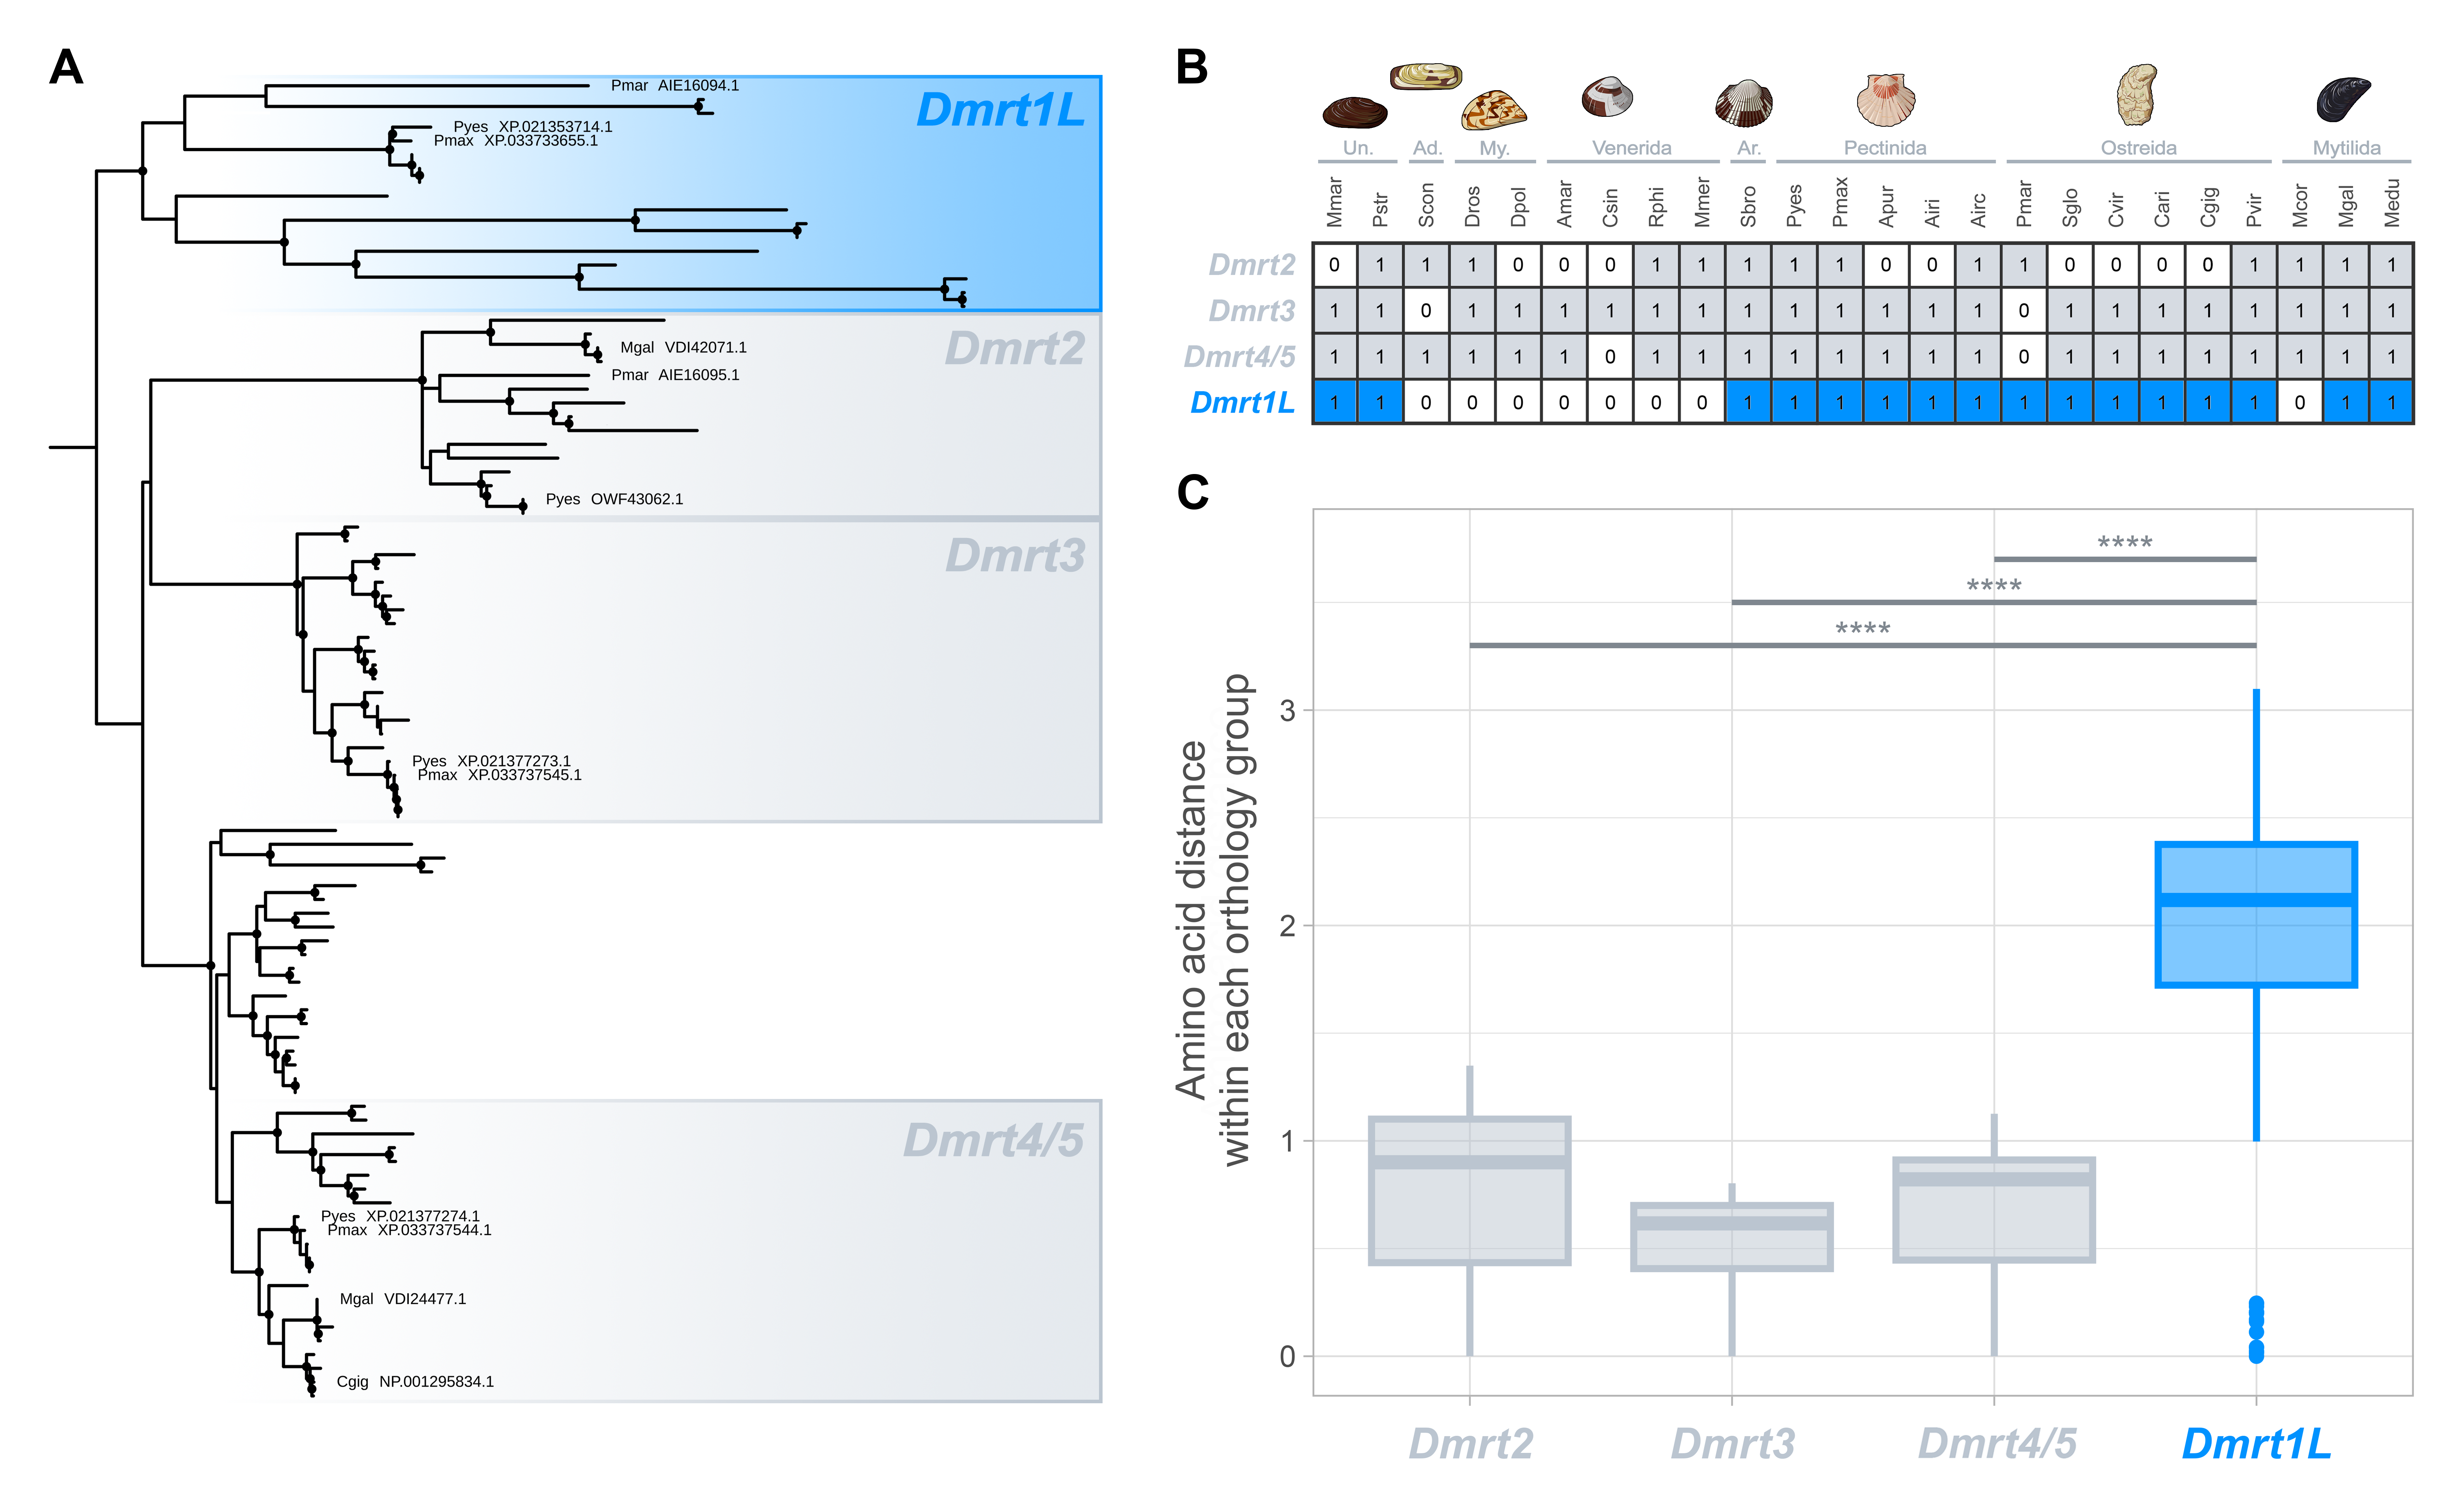
\includegraphics[width=\textwidth]{chapter2/fig_2.png}
    \captionsetup{width=\textwidth}
    \caption{
    \textbf{Phylogenetic tree (A) and taxonomic distribution (B) of \textit{Dmrt} genes in bivalves, and comparison of amino acid pairwise distances within \textit{Dmrt1L} and the other \textit{Dmrt}s (B)}. (A) \textit{Dmrt} orthologs from bivalve genome assemblies were obtained with HMMsearch (HMMER toolkit; \textbf{\cite{eddy2011accelerated}}) with the Pfam HMM profile of the DM domain (PF00751). Amino acid alignment was obtained with MAFFT-DASH (\textbf{\cite{rozewicki2019mafft}}), and manually inspected to remove poorly aligning sequences, and trimmed with trimAl (gap threshold of 60\%; \textbf{\cite{capella2009trimal}}). The phylogenetic analysis was carried out using IQ-TREE 2 (\textbf{\cite{minh2020iq}}) with default parameters. Nodes with bootstrap values greater than 84 are marked with filled black circles. The tree was rooted according to \textbf{\cite{evensen2022comparative}}. \textit{Dmrt} genes analysed by \textbf{\cite{evensen2022comparative}} were used as reference to annotate the various orthology groups, and accession numbers are reported in the tree. The phylogenetic tree with all annotated tips and nodes can be accessed on supplementary material online. (B) Taxonomic distribution of identified \textit{Dmrt} genes in bivalve genomes. Orders as reported in WoRMS (accessed before or on 14/03/2023) and in \textbf{Figure \ref{fig:summarySex}} are specified. (C) Pairwise amino acid distances were computed for amino acid sequences within each Dmrt orthology group identified in the tree, with the R package ‘phangorn’ (\textbf{\cite{schliep2011phangorn}}) under the JTT substitution model. After checking for normality with the Shapiro-Wilk test (W = 0.88544, p-value < 2.2e-16) and for group effect with the Kruskal-Wallis test (p-value < 2.2e-16), the pairwise Wilcoxon rank-sum test was used to compare the distributions of pairwise amino acid distances of Dmrt1L and the other Dmrts. Horizontal bars mark the significative results with p < 2.2e-16 (‘****’) (Bonferroni correction for multiple test was applied). The list of genome assemblies used for these analyses and species identifiers can be found in \textbf{Figure \ref{tab:genomes}}. Un.: Unionida; Ad.: Adapedonta; My.: Myida; Ar.: Arcida.
    }
    
    \label{fig:dmrt}
\end{figure}

The present analysis also supports a higher amino acid sequence divergence of the \textit{Dmrt1L} orthology group with respect to the other \textit{Dmrt} orthology groups (\textbf{Figure \ref{fig:summarySex}C}), which may be explained by a higher rate of sequence evolution related to their sex-biased expression in certain species (\textbf{\cite{zhang2014genomic,shi2015novo,li2018foxl2,evensen2022comparative}}). This is consistent with what has been already observed for the SRGs \textit{Dmrt1} and \textit{dsx} in vertebrates and \textit{Drosophila}, respectively (e.g., \textbf{\cite{bewick2011evolution,baral2019genetic}}). In fact, sex-biased genes (including SRGs) often tend to evolve faster than unbiased genes at the level of protein sequences, either when considering male-biased (reviewed in \textbf{\cite{parsch2013evolutionary,grath2016sex}}) or female-biased genes (e.g., \textbf{\cite{papa2017rapid,ghiselli2018comparative}}). Another possible explanation for the higher amino acid divergence of \textit{Dmrt1L} genes may lie on their expression breadth, that is, genes with a narrow tissue-specific expression tend to evolve faster than more ubiquitous genes (\textbf{\cite{parsch2013evolutionary,xu2022multi}}). As a matter of fact, \textit{Dmrt1L} genes have been found to be significantly more transcribed in the gonadic tissue (particularly in testes) in \textit{P. yessoensis} (\textbf{\cite{li2018foxl2}}) and \textit{C. gigas} (\textbf{\cite{yue2021variance}}).

Understanding the role and molecular interactions of \textit{Dmrt1L} genes in bivalve SD and gonad development would greatly enhance the possibility of outlining the evolutionary causes and consequences of their high amino acid divergence (\textbf{Figure \ref{fig:dmrt}C}), for example by linking the molecular evolution to the degree of pleiotropy. However, most of our knowledge on \textit{Dmrt1L} biology is currently limited to the temporal and tissue localization of transcripts in a few species of bivalves (e.g., \textbf{\cite{li2018foxl2,yue2021variance}}). In fact—apart from the work by \textbf{\cite{sun2022examination}}, which confirmed the role of \textit{Dmrt1L} in the gonad development of \textit{C. gigas} through non-invasive RNAi and found that the knocked-down phenotype results in size reduction of male gonads—no other experiments intended to elucidate the function of \textit{Dmrt1L} genes in bivalves have been carried out so far (\textbf{Figure \ref{fig:summarySex}}). This clearly hinders any possible integration between molecular data with functional assays.
If the role of \textit{Dmrt1L} as major sex determinants was confirmed, bivalves would become an intriguing clade in which investigate why, in Metazoa, certain genes (namely, the \textit{Dmrt} gene family) appear particularly prone to being recruited at the top of the SD cascade. To date, this phenomenon has been widely examined in vertebrates, where \textit{Dmrt1} genes have independently gained a primary role in male SD in fish, amphibians, and birds, and are considered candidate sex-determining genes also in monotreme mammals (\textbf{\cite{marshall2010homologies,beukeboom2014evolution,mawaribuchi2019independent}}). Bivalves may provide an alternative evolutionary scenario to study the selective forces and molecular modifications that support \textit{Dmrt} genes in repeatedly taking over the SD process. In fact, since \textit{Dmrt1L} genes seem to be restricted to molluscs (\textbf{Figure \ref{fig:dmrt}A}), it would be intriguing to clarify if the putative involvement in the SD cascade of extant bivalve species is the result of shared ancestry or convergent evolution, which would establish a study system for the evolution of \textit{Dmrt} genes parallel to that of vertebrates (see \textbf{\cite{capel2017vertebrate}}).

Obviously, \textit{Dmrt1L} should not be expected to be the sole sex-determining gene. In fact, \textit{FoxL2} has already been appointed as the female sex-determining gene in \textit{P. yessoensis} and \textit{C. farreri} (\textbf{\cite{han2022ancient}}). Consequently, we should expect that other primary genetic determinants exist, consistently with the extremely high species diversity of the clade. Thus, bivalves may additionally serve as a valuable model system to study how genes from different families take over the SD cascade and are shaped by selection.

\section{Conclusions: bivalves as new models in the study of sex determination}
SD is undoubtedly a fascinating biological and evolutionary topic as much as it is challenging to investigate. Our understanding of the causes and consequences of the SD mechanism diversity strongly relies on the study of different systems and non-model model organisms (\textbf{\cite{bachtrog2014sex,milani2020faraway}}), which provide the foundation for depicting a comprehensive evolutionary and comparative framework in which new and coherent research perspectives can be grounded.

In recent years, bivalves have been achieving growing importance in many fields of biology, from ecology to genomics, and from environmental biomonitoring to mitochondrial studies (\textbf{\cite{milani2020faraway,ghiselli2021bivalve}}), but they can be a valuable model to address also SD studies. The diversity of their life history traits provides indeed a challenging, yet extremely fascinating framework, to put the SD processes into an evolutionary context.

Bivalves can help us explain how ESD and GSD interplay with each other in response to the environmental conditions, as a mixed system of both has been proposed to act in the establishment of bivalve sexual identity (reviewed in \textbf{\cite{breton2018sex}}). Moreover, the occurrence of the many existing variants of hermaphroditism and gonochorism even in closely related species, or within the same population, strongly suggests that the basic SD pathway (whether genetic, environmental, or mixed) should be plastic enough to sustain the existence of individuals of both sexes, thus providing the opportunity to study how SD gene regulatory networks are shaped and selected throughout evolution and how epigenetic regulation may influence SD. The unique DUI system further poses an undeniable challenge in SD studies since it may represent an SD-linked mechanism which relies on the non-nuclear portion of the genome and may unfold many new research paths (\textbf{\cite{milani2020faraway,ghiselli2021bivalve}}). Nonetheless, much of the research effort on bivalve SD has been devolved to specific groups of socio-economic importance, such as Mytilida, Ostreida, Pectinida, and Unionida, while the other lineages of the bivalve phylogeny have been neglected (\textbf{Figure \ref{fig:summarySex}}). Our understanding of the SD processes of bivalves is thus restricted and is mainly lacking a broad comparative framework in which to draw comprehensive evolutionary inferences. 

Genes from the \textit{Dmrt}, \textit{Sox} and \textit{Fox} families, which are involved in SD also in other Metazoa, may be considered excellent genomic targets to study the processes and patterns of molecular evolution in sex-biased genes, as well as of the recurrent recruitment of genes in the SD cascade. Also, identifying the major genetic regulators of SD in bivalves would burst the functional study of the interaction between ESD and GSD, by providing genetic targets that can be manipulated through RNAi and/or genome editing techniques to understand the role of environmental cues in SD. In the same way, knowing the main genetic actors of SD would allow researcher to identify SCs not only on the basis of in-silico techniques (such as k-mer based or SNP methods) but also by less-expensive wet lab protocols (such as fluorescence in situ hybridization on metaphase chromosome plates). Furthermore, it would help to understand whether and how the mitochondrial additional ORFs of DUI species interact with the SD system, by performing thorough gene expression essays.

In conclusion, we strongly urge researchers to invest more resources in the integrative study of bivalve SD to unravel the many underlying mechanisms and expand our understanding of this biological process. Given our limited knowledge in the field, one of the first routes that should be undertaken may rely on the comparative study of SRGs of bivalves from a genomic perspective, as this kind of data is nowadays growing at a rate faster than ever. Establishing such a genomic ground plan for understudied organisms will in fact allow researchers to develop evolutionary-aware experiments with better selected genetic targets.

\begin{landscape}
\footnotesize
\begin{longtable}{@{}lllllll@{}}
\caption{\textbf{List of bivalve genomes from which \textit{Dmrt} genes have been extracted.} For each species, the accepted name and the most-common synonym (in parentheses) are reported. NCBI accession numbers are provided, when available, as well as BUSCO scores of the predicted proteomes against the metazoa\_odb10 dataset (\textbf{\cite{manni2021busco}}).}
\label{tab:genomes}\\
\toprule
\textbf{Species} &
  \textbf{ID} &
  \textbf{Order} &
  \textbf{Assembly level} &
  \textbf{BUSCO score} &
  \textbf{Reference} &
  \textbf{NCBI Acc. No.} \\* \hline \hline
\endfirsthead
%
\multicolumn{7}{c}%
{{\bfseries Table \thetable\ continued from previous page}} \\
\toprule
\textbf{Species} &
  \textbf{ID} &
  \textbf{Order} &
  \textbf{Assembly level} &
  \textbf{BUSCO score} &
  \textbf{Reference} &
  \textbf{NCBI Acc. No.} \\* \hline \hline
\endhead
%
\endfoot
%
\endlastfoot
%
\textit{Anadara (Scapharca) broughtonii} &
  Sbro &
  Arcida &
  Chromosome &
  \begin{tabular}[c]{@{}l@{}}C:91.2\%\\ {[}S:85.6\%,D:5.6\%{]}\\ F:2.6\%\\ M:6.2\%\end{tabular} &
  \textbf{\cite{bai2019chromosomal}} &
  NA \\* \midrule
\textit{Sinonovacula constricta} &
  Scon &
  Adapedonta &
  Chromosome &
  \begin{tabular}[c]{@{}l@{}}C:92.5\%\\ {[}S:80.4\%,D:12.1\%{]}\\ F:3.4\%\\ M:4.1\%\end{tabular} &
  \textbf{\cite{ran2019chromosome}} &
  GCA\_007844125.1 \\* \midrule
\textit{Dreissena polymorpha} &
  Dpol &
  Myida &
  Chromosome &
  \begin{tabular}[c]{@{}l@{}}C:86.9\%\\ {[}S:75.1\%,D:11.8\%{]}\\ F:6.4\%\\ M:6.7\%\end{tabular} &
  \textbf{\cite{mccartney2022genome}} &
  GCA\_020536995.1 \\* \midrule
\textit{Dreissena rostriformis} &
  Dros &
  Myida &
  Scaffold &
  \begin{tabular}[c]{@{}l@{}}C:75.2\%\\ {[}S:73.2\%,D:2.0\%{]}\\ F:15.2\%\\ M:9.6\%\end{tabular} &
  \textbf{\cite{calcino2019quagga}} &
  GCA\_007657795.1 \\* \midrule
\textit{Mytilus unguiculatus (coruscus)} &
  Mcor &
  Mytilida &
  Chromosome &
  \begin{tabular}[c]{@{}l@{}}C:80.0\%\\ {[}S:79.1\%,D:0.9\%{]}\\ F:7.7\%\\ M:12.3\%\end{tabular} &
  \textbf{\cite{yang2021chromosome}} &
  GCA\_017311375.1 \\* \midrule
\textit{Mytilus edulis} &
  Medu &
  Mytilida &
  Scaffold &
  \begin{tabular}[c]{@{}l@{}}C:83.7\%\\ {[}S:64.5\%,D:19.2\%{]}\\ F:5.2\%\\ M:11.1\%\end{tabular} &
  \textbf{\cite{corrochano2022evidence}} &
  GCA\_905397895.1 \\* \midrule
\textit{Mytilus galloprovincialis} &
  Mgal &
  Mytilida &
  Scaffold &
  \begin{tabular}[c]{@{}l@{}}C:80.3\%\\ {[}S:47.5\%,D:32.8\%{]}\\ F:8.8\%\\ M:10.9\%\end{tabular} &
  \textbf{\cite{gerdol2020massive}} &
  GCA\_900618805.1 \\* \midrule
\textit{Perna viridis} &
  Pvir &
  Mytilida &
  Scaffold &
  \begin{tabular}[c]{@{}l@{}}C:99.4\%\\ {[}S:99.0\%,D:0.4\%{]}\\ F:0.2\%\\ M:0.4\%\end{tabular} &
      \textbf{\cite{inoue2021genomics}} &
  GCA\_018327765.1 \\* \midrule
\textit{Magallana (Crassostrea) ariakensis} &
  Cari &
  Ostreida &
  Chromosome &
  \begin{tabular}[c]{@{}l@{}}C:94.6\%\\ {[}S:90.9\%,D:3.7\%{]}\\ F:0.9\%\\ M:4.5\%\end{tabular} &
  \textbf{\cite{li2021genome}} &
  GCA\_020567875.1 \\* \midrule
\textit{Magallana (Crassostrea) gigas} &
  Cgig &
  Ostreida &
  Chromosome &
  \begin{tabular}[c]{@{}l@{}}C:98.5\%\\ {[}S:67.6\%,D:30.9\%{]}\\ F:0.3\%\\ M:1.2\%\end{tabular} &
  \textbf{\cite{penaloza2021chromosome}} &
  GCF\_902806645.1 \\* \midrule
\textit{Crassostrea virginica} &
  Cvir &
  Ostreida &
  Chromosome &
  \begin{tabular}[c]{@{}l@{}}C:98.1\%\\ {[}S:58.6\%,D:39.5\%{]}\\ F:0.3\%\\ M:1.6\%\end{tabular} &
  \textbf{\cite{gomez2015developing}} &
  GCF\_002022765.2 \\* \midrule
\textit{Saccostrea glomerata} &
  Sglo &
  Ostreida &
  Scaffold &
  \begin{tabular}[c]{@{}l@{}}C:88.9\%\\ {[}S:85.3\%,D:3.6\%{]}\\ F:5.1\%\\ M:6.0\%\end{tabular} &
  \textbf{\cite{powell2018genome}} &
  GCA\_003671525.1 \\
\textit{Argopecten irradians concentricus} &
  Airc &
  Pectinida &
  Scaffold &
  \begin{tabular}[c]{@{}l@{}}C:94.8\%\\ {[}S:93.9\%,D:0.9\%{]}\\ F:3.7\%\\ M:1.5\%\end{tabular} &
  \textbf{\cite{liu2020draft}} &
  GCA\_004382765.1 \\* \midrule
\textit{Argopecten irradians irradians} &
  Airi &
  Pectinida &
  Scaffold &
  \begin{tabular}[c]{@{}l@{}}C:94.8\%\\ {[}S:93.9\%,D:0.9\%{]}\\ F:3.7\%\\ M:1.5\%\end{tabular} &
  Liu et al., 2020 &
  GCA\_004382745.1 \\* \midrule
\textit{Argopecten purpuratus} &
  Apur &
  Pectinida &
  Scaffold &
  \begin{tabular}[c]{@{}l@{}}C:89.2\%\\ {[}S:88.5\%,D:0.7\%{]}\\ F:5.0\%\\ M:5.8\%\end{tabular} &
  \textbf{\cite{liu2020draft}}
  NA \\* \midrule
\textit{Pecten maximus} &
  Pmax &
  Pectinida &
  Chromosome &
  \begin{tabular}[c]{@{}l@{}}C:98.5\%\\ {[}S:74.7\%,D:23.8\%{]}\\ F:0.4\%\\ M:1.1\%\end{tabular} &
  \textbf{\cite{kenny2020gene}} &
  GCF\_902652985.1 \\* \midrule
\textit{Mizuhopecten (Patinopecten) yessoensis} &
  Pyes &
  Pectinida &
  Scaffold &
  \begin{tabular}[c]{@{}l@{}}C:98.6\%\\ {[}S:75.2\%,D:23.4\%{]}\\ F:0.4\%\\ M:1.0\%\end{tabular} &
  \textbf{\cite{wang2017scallop}} &
  GCF\_002113885.1 \\* \midrule
\textit{Margaritifera margaritifera} &
  Mmar &
  Unionida &
  Scaffold &
  \begin{tabular}[c]{@{}l@{}}C:92.6\%\\ S:82.3\%,D:10.3\%{]}\\ F:3.2\%\\ M:4.2\%\end{tabular} &
  \textbf{\cite{gomes2021crown}} &
  GCA\_015947965.1 \\* \midrule
\textit{Potamilus streckersoni} &
  Pstr &
  Unionida &
  Scaffold &
  \begin{tabular}[c]{@{}l@{}}C:74.7\%\\ {[}S:73.8\%,D:0.9\%{]}\\ F:7.0\%\\ M:18.3\%\end{tabular} &
  \textbf{\cite{smith2021high}} &
  GCA\_016746295.1 \\* \midrule
\textit{Calyptogena (Archivesica) marissinica} &
  Amar &
  Venerida &
  Chromosome &
  \begin{tabular}[c]{@{}l@{}}C:82.0\%\\ {[}S:80.0\%,D:2.0\%{]}\\ F:6.1\%\\ M:11.9\%\end{tabular} &
  \textbf{\cite{ip2021host}} &
  GCA\_014843695.1 \\* \midrule
\textit{Cyclina sinensis} &
  Csin &
  Venerida &
  Scaffold &
  \begin{tabular}[c]{@{}l@{}}C:94.0\%\\ {[}S:83.8\%,D:10.2\%{]}\\ F:1.9\%\\ M:4.1\%\end{tabular} &
  \textbf{\cite{wei2020chromosome}} &
  GCA\_012932295.1 \\* \midrule
\textit{Mercenaria mercenaria} &
  Mmer &
  Venerida &
  Chromosome &
  \begin{tabular}[c]{@{}l@{}}C:95.4\%\\ {[}S:70.9\%,D:24.5\%{]}\\ F:0.5\%\\ M:4.1\%\end{tabular} &
  \textbf{\cite{song2021hard}} &
  GCF\_014805675.1 \\* \midrule
\textit{Ruditapes   philippinarum} &
  Rphi &
  Venerida &
  Chromosome &
  \begin{tabular}[c]{@{}l@{}}C:83.4\%\\ {[}S:74.5\%,D:8.9\%{]}\\ F:8.8\%\\ M:7.8\%\end{tabular} &
  \textbf{\cite{xu2022multi}} &
  GCA\_026571515.1 \\* \bottomrule \bottomrule
\end{longtable}
\end{landscape}

\section{Acknowledgments}
The authors are extremely thankful to Sofía Blanco González from the University of Vigo for her willingness to engage in discussions and for genuinely sharing her opinion on this work.

\section{Data Availability}
Analyzed data and R scripts used to generate plots can be accessed in supplementary material online deposited at the following GitHub repository: \href{https://github.com/filonico/bivalve_sex_perspective}{filonico/bivalve\_sex\_perspective}.

\end{document}
\documentclass[../main.tex]{subfiles}

\begin{document}

{
\setstretch{1.0}
\chapter{Identification of putative sex-determination related genes in bivalves through comparative molecular evolutionary analyses}
\label{molecularEvolution}

\noindent{\Large{Filippo Nicolini\textsuperscript{1,2}, Mariangela Iannello\textsuperscript{1}, Giovanni Piccinini\textsuperscript{1}, Sergey Nuzhdin\textsuperscript{3}, Fabrizio Ghiselli\textsuperscript{1}, Andrea Luchetti\textsuperscript{1}, Liliana Milani\textsuperscript{1}}}

\vspace{5mm}

\noindent{\textsuperscript{1}\textit{Department of Biological, Geological and Environmental Science, University of Bologna, Bologna (BO), Italy}.}

\noindent{\textsuperscript{2}\textit{Fano Marine Center, Fano (PU), Italy}.}

\noindent{\textsuperscript{3}\textit{Department of Molecular and Computational Biology, University of Southern California, Los Angeles, CA, USA}.}

\vspace{5mm}

\noindent{\large{\textbf{\textit{In preparation.}}}}
}

\newpage

\section{Introduction} \label{chapter3_introduction}
In sexually reproducing organisms, the modes of \gls{sd}, i.e., the process by which the male or female identity of an organism (or of the gonadic tissue) is established, is highly diverse, ranging from strictly genetic systems to environmentally-dependent processes (\textbf{\cite{haag2005sex, uller2011origin, bachtrog2014sex, beukeboom2014evolution}}). Characterising the molecular basis of \gls{sd} is crucial for understanding not only reproductive biology but also the evolutionary pressures shaping these systems (\textbf{\cite{wilkins1995moving, ellegren2007evolution, grath2016sex, nicolini2023bivalves}}), as \glspl{srg}, including primary \glspl{sdg}, are those responsible for the phenotypic differences of males and females, thanks to their sex-biased expression and interactions (\textbf{\cite{ellegren2007evolution, beukeboom2014evolution, grath2016sex}}). One key aspect of \glspl{srg} is that they often exhibit accelerated rates of sequence evolution, due to their involvement in sex-related traits and reproduction. This represents the effects of sexual and/or adaptive selection, which act in sex-biased genes and produce high-divergent proteins at the interspecific level (\textbf{\cite{civetta1998sex, ellegren2007evolution, meisel2011towards, grath2016sex}}). Rapid sequence evolution is known for \gls{sry} of therians (\textbf{\cite{pamilo1997evolution, mawaribuchi2012molecular}}), \gls{dmw} of the African clawed frog \gls{xlae}, and \gls{dmy} of the medaka fish \gls{olat} (\textbf{\cite{mawaribuchi2012molecular}}), all of which are master \glspl{sdg}, that is, genes whose expression is primarly responsible for the establishment of the sexual fate of the organism. Evolution under episodic diversifying selection has been detected also in \textit{Drosophila} for genes involved in the \gls{sd} cascade [e.g., \gls{sxl}, \gls{tra}, and \gls{dsx}], in correspondence with its establishment in the genus common ancestor (\textbf{\cite{mullon2012drosophila_sxl, baral2019genetic}}); though, rapid sequence evolution seems to not be concerning extant amino acid sequences (\textbf{\cite{haerty2007evolution, baral2019genetic}}), as they are globally evolving under purifying selection, especially in their catalytic domain (\textbf{\cite{mullon2012drosophila_sxl, baral2019genetic}}). Concerning the \gls{dsx} genes, higher rates of nucleotide and amino acid sequence evolution can be however observed for male-specific regions, if compared to female-specific and oligomerization regions (\textbf{\cite{baral2019genetic}}).

While \gls{sd} has been extensively studied in model organisms, like mammals, insects, and nematodes, comparatively little is known about the molecular ground plans in non-model organisms. A remarkable example of this is represented by bivalve molluscs, which exhibit a wide variety of reproductive strategies and sexual systems (\textbf{\cite{breton2018sex}}). Notwithstanding the considerable importance in the human socio-economic landscape (reviewed in \textbf{\cite{haszprunar2012molluscs, gomes2020molluscan}}), the study of \gls{sd} mechanisms in bivalves has been hampered by the striking divergence among species (\textbf{\cite{li2022sex}}), and thus largely overlooked and limited to few case studies (\textbf{\cite{breton2018sex, nicolini2023bivalves}}). So far, no master \gls{sdg} has been unambiguously identified, and the only working hypothesis on the functioning of the \gls{sd} gene regulatory network is available for the Pacific oyster \gls{cgig} (now \textit{Magallana gigas}; \textbf{\cite{zhang2014genomic}}). Nonetheless, the field still lacks both a robust functional investigation and an evolutionary framework in which to place the current knowledge (\textbf{\cite{nicolini2023bivalves}}). As a matter of fact, major efforts have been dedicated to identify sex-biased genes through \gls{dge} analyses (e.g., \textbf{\cite{milani2013nuclear, teaniniuraitemoana2014gonad, zhang2014genomic, capt2018deciphering, afonso2019gonad}}), but very few have leveraged cutting-edge techniques to investigate their actual role in \gls{sd} and/or gonad differentiation and development (e.g., \textbf{\cite{liang2019sox2, sun2022examination}}).

Components of the \gls{dsfg} families are notoriously known as key actors in several developmental processes across Metazoa (\textbf{\cite{benayoun2011forkhead, matson2012sex, sarkar2013sox, mawaribuchi2019independent}}), including \gls{sd} in certain clades: the aforementioned \gls{dmw}, \gls{dmy}, and \gls{dsx} all belong to the \gls{dmrt} gene family, while \gls{sry} belongs to the \gls{sox} gene family; \textit{Fox-L2}, which takes part in most of the vertebrate \gls{sd} processes as a downstream effector of the female pathway, belongs to the \gls{fox} gene families. Members of the \glspl{dsfg} have been identified as putative \glspl{srg} also in bivalves, thanks to both \gls{dge} analyses and \gls{ish} (e.g., \textbf{\cite{naimi2009molecular, li2018foxl2, liang2019sox2, yue2021variance}}), suggesting that their role in morphological and sexual development is maintained also in the clade. However, the clear role of DSFGs has yet to be elucidated, probably as a consequence to the lack of (i) a systematic classification of the families and (ii) a comprehensive understanding of their evolutionary history.

In order to overcome such limitations, this study aims to perform a thorough investigation of the \gls{dsfg} families in bivalves, with the attempt to provide a high-quality resource to be used as a reference for future studies. Through the analysis of more than 40 annotated bivalve genomes and transcriptomes, we aim (i) to describe the complete set and evolutionary history of \glspl{dsfg} in bivalves by means of phylogenetic inferences, manual curation, and orthology prediction; furthermore, we aim (ii) to identify \glspl{dsfg} potentially involved in bivalve \gls{sd} by investigating their sequence evolution in a genome-wide context. As a matter of fact, our hypothesis is that, if any of the \glspl{dsfg} is directly involved in \gls{sd} (i.e., is a \gls{sdg}), then we should expect it to be experiencing a higher rate of sequence evolution, as already found in previous studies (\textbf{\cite{pamilo1997evolution, mawaribuchi2012molecular}}) and discussed earlier; this characteristic, in turn, would be reflected in a high diversity of the extant amino acid sequences across the bivalve clade. To assess the robustness and reliability of our approach, we additionally applied our pipeline to two non-bivalve datasets, composed of mammal and \textit{Drosophila} species, respectively (hereon referred to as the ‘mammal dataset’ and the ‘fruit fly dataset’). By choosing two clades for which \gls{sd} is well characterised, we wanted to compare our results with those obtained on taxa for which a deeper and detailed knowledge is available. Particularly, mammals and \textit{Drosophila} provide two different frameworks to study the patterns of molecular evolution in \glspl{sdg}: the former is a system where \gls{sd} is completely genetic (i.e., the development into a male or into a female is triggered by the up- or downregulation of \gls{sry} in undifferentiated gonads, respectively), while the latter is a system where \gls{sd} is chromosomic, thus lacks a master \gls{sdg} (the sexual fate of the individual is determined by the ratio between autosomal and X chromosomes). Hence, they represent opposing control datasets to be compared to bivalves, as it is expected that a higher rate of sequence evolution concerns only master \glspl{sdg} (as \gls{sry} in therians; i.e., the top regulatory part of the \gls{sd} cascade), but not also the downstream genes (i.e., the bottom effectors). If our method is robust, we should thus expect that, (i) in the mammalian dataset \gls{sry} is detected as rapidly-evolving, while (ii) in the fruit fly dataset no gene among those working within the sex-determining cascade is evolving at a higher pace. By testing the performance of the pipeline in mammals and fruit flies, we were able to assess the reliability of results in bivalves.

This work offers novel insights into the evolutionary dynamics of \glspl{srg} and contributes a valuable genomic resource for understanding \gls{sd} in bivalves, one of the most ecologically and economically important groups of marine organisms. Particularly, here we provide the first extensive phylogenetic-based classification of \glspl{dsfg} in bivalves, covering many species from the major bivalve orders, along with a comprehensive investigation of their sequence evolution.

\section{Materials and Methods} \label{chapter3_MM}
\subsection{Dataset of bivalve annotated genomes and transcriptomes}
Annotated genome assemblies of bivalves were obtained from various publicly available resources, while reference genome assemblies for gastropods and cephalopods were downloaded from NCBI (\textbf{Supp. Tab. \ref{suppTab:bivalve_dataset}}). Isoforms were removed from genome annotations using a perl script from the AGAT toolkit (v0.8.0; \textbf{\cite{dainat2022another}}). Concerning \gls{scon} (Adapedonta), the nucleotide coding sequence fasta file was not available for download. To avoid excluding the species from our analyses, the file was generated in-house by mapping the annotated protein sequences on the reference genome using miniprot (v0.13-0; \textbf{\cite{li2023miniprot}}). Then, the corresponding nucleotide sequences were extracted using AGAT on the resulting gff annotation file.

In order to provide an extensive identification of \glspl{srg} also for underrepresented bivalve orders (mainly belonging to the Heterodonta clade), 14 additional species represented by sequenced transcriptomes were included in the analyses. Assembled and annotated transcriptomes were obtained from \textbf{\cite{piccinini2021mitonuclear}} and \textbf{\cite{iannello2023signatures}}. Briefly, raw reads were trimmed using Trimmomatic (\textbf{\cite{bolger2014trimmomatic}}) and assembled using Trinity (\textbf{\cite{grabherr2011trinity}}) with default parameters. Isoforms were removed using the dedicated perl script from the Trinity utilities. Open reading frames were predicted through TransDecoder (\textbf{\cite{haasTransdecoder}}), by also including diamond (\textbf{\cite{buchfink2015fast}}) and HMMER (v3.3.2; http://hmmer.org/) annotation of hits.

The resulting set of annotated genomes and transcriptomes (hereafter referred to as the “comprehensive set”) was checked for completeness using BUSCO with the Metazoa reference dataset (v5.2.2; \textbf{\cite{manni2021busco}}).

\subsection{Identification and classification of Dmrt, Sox and Fox genes in bivalves}
Members of \gls{dsfg} families were retrieved in the comprehensive set with hmmsearch from the HMMER package (v3.3.2; http://hmmer.org/). The signature catalytic domains of each family were used as queries. Specifically, \gls{hmm} profiles were built after the Pfam databases for the \gls{dm} domain (PF00751), the \gls{hmg} box (PF00505) and the forkhead domain (PF00250) to retrieve members of the \gls{dsfg} families, respectively. The e-value for both the per-target and the per-domain inclusion threshold was set to $\num{1.0e-5}$.

Obtained hits were then annotated using (i) the PANTHER HMM standalone sequence scoring against the PANTHER library v18.0 and (ii) RPS-BLAST (v2.5.0+) against the Conserved Domain Database (CDD; pre-compiled version, downloaded from \href{https://ftp.ncbi.nih.gov/pub/mmdb/cdd/little_endian/}{ftp.ncbi.nih.gov} on 09/11/23). In both cases, hits with an e-value of $\num{1.0e-5}$ were retained. Genes which were correctly annotated by both systems (on the basis of the PANTHER gene family and CDD domain identifiers; \textbf{Supp. Tab. \ref{suppTab:panther_cdd}}) were kept for subsequent analyses.

\glspl{dsfg} from \gls{hsap}, \gls{dmel}, and \gls{cele} (\textbf{Supp. Tab. \ref{suppTab:reference_dsfgs}}; hereafter referred to as ‘reference species’) were retrieved from NCBI and were used as reference genes for annotation (see below). Classification and nomenclature of each family was retrieved from: \textbf{\cite{mawaribuchi2019independent}} for \gls{dmrt} genes; \textbf{\cite{phochanukul2010no}} and \textbf{\cite{sarkar2013sox}} for \gls{sox} genes; \textbf{\cite{mazet2003phylogenetic}} for \gls{fox} genes.

The alignments of mollusc and reference \glspl{dsfg} were guided by the aforementioned Pfam \gls{hmm} profiles and performed with Clustal Omega (v1.2.3; \textbf{\cite{sievers2011fast}}), then trimmed with trimAl (v1.4.rev15; \textbf{\cite{capella2009trimal}}) with a gap threshold of 40\%. Resulting alignments were manually inspected to remove sequences with incomplete catalytic domains, then aligned and trimmed again as before. Phylogenetic trees were inferred using IQ-TREE (v2.1.4-beta COVID-edition; \textbf{\cite{minh2020iq}}) with automatic model selection (\textbf{\cite{kalyaanamoorthy2017modelfinder}}), 1000 bootstrap replicates and 5 independent runs. The phylogenetic tree of \gls{dmrt} genes was midpoint rooted, as no clear homology relationship has been found with other gene families or zinc-finger proteins so far (\textbf{\cite{wexler2014pan}}). Phylogenetic trees of \gls{sox} and \gls{fox} gene families were rooted using two fungi mating protein A (Mat-A) sequences (XP\_62685912.1, CCD57795.1) and two Amoebozoa forkhead-like domains (XP\_004368148.1, XP\_004333268.1), respectively (\textbf{\cite{heenan2016evolution,nakagawa2013dna}}). The rooting was performed with Gotree (v0.4.5; \textbf{\cite{lemoine2021gotree}}). To identify and annotate bivalve homology groups within each gene family, we employed a species overlap algorithm followed by a \gls{mcl} weighted by node supports as implemented in Possvm (v1.2; \textbf{\cite{grau2021orthology}}). \glspl{dsfg} from \gls{hsap}, \gls{dmel}, and \gls{cele} were used as reference annotation.

In order to better establish the orthology relationships among ambiguous groups of \gls{dmrt} and \gls{fox} genes, we run a series of other phylogenetic reconstructions (see \ref{chpater3_discussion}), by using the same pipeline as before. In the case of \textit{Fox-Y} genes, we also employed Fox gene sequences from the sea urchin \gls{spur}, as given by \textbf{\cite{tu2006sea}}. All the phylogenetic trees were plotted using the R package ‘ggtree’ (\textbf{\cite{yu2017genome}}).

\subsection{Sequence diversity of bivalve single-copy orthogroups}
As a metrics to measure the sequence diversity of bivalve \glspl{dsfg}, and test whether those putatively involved in \gls{sd} show higher values than other genes, we employed the amino acid sequence divergence. As a matter of fact, this metric is fast and straightforward to obtain, as it only requires the amino acid alignment and the corresponding best-fit substitution mode.

To this purpose, we produced amino acid alignments of bivalve \glspl{sco} groups and built the distribution of their median \gls{aasd}. Specifically, we assembled a second dataset (hereafter referred to as the ‘reduced bivalve dataset’) which includes, for each bivalve genus, only the best genomes and transcriptomes in terms of either BUSCO scores (on the metazoan\_odb10 dataset; \textbf{\cite{manni2021busco}}) or assembly statistics (\textbf{Supp. Tab. \ref{suppTab:bivalve_dataset}}), in order to reduce computational time. \gls{amar} (now \textit{Calyptogena marissinica}) and \gls{sglo} were also removed, as their annotated coding sequences contain many stop codons, which prevent accurate amino acid guided alignments. Genes were clustered in orthologous groups using OrthoFinder (v2.5.5; \textbf{\cite{emms2019orthofinder}}) with DIAMOND ultra-sensitive and default parameters. Resulting orthogroups were splitted into \glspl{sco} using DISCO (v1.3.1; \textbf{\cite{willson2022disco}}), and orthogroups with at least 17 species (50\% of the species included in the bivalve reduced dataset) were retained. Amino acid and nucleotide sequences of \glspl{sco} were then aligned using Clustal Omega as implemented in TranslatorX (v1.1; \textbf{\cite{abascal2010translatorx}}), and jointly trimmed using trimAl with a gap threshold of 40\% and the removal of spurious sequences (\verb|-resoerlap 50 -seqoverlap 50|). Eventually, orthogroups containing (i) internal stop codons, (ii) with less than 17 species left (50\% of the species included in the bivalve reduced dataset), or (iii) containing DSFGs were removed from downstream analyses. The best amino acid substitution model was inferred for each trimmed alignment using ModelFinder as implemented in IQTREE2 (model search was restricted to matrices accepted by the ‘phangorn’ R library; i.e., Blosum62, cpREV, Dayhoff, DCMut, FLU, HIVb, HIVw, JTT, JTTDCMut, LG, mtART, mtMAM, mtREV, mtZOA, rtREV, VT, WAG) and the corresponding pairwise amino acid distances were computed with the function ‘dist.ml’ from the ‘phangorn’ R package (\textbf{\cite{schliep2011phangorn}}). We decided to employ the pairwise amino acid distance instead of the tip-to-tip phylogenetic distance (which accounts for a more comprehensive evolutionary signal) in order to save computational time. However, to check whether the two metrics were comparable to each other, we randomly selected 200 decomposed orthogroups (including orthogroups from the \glspl{dsfg}) and computed the \gls{ml} trees using IQTREE2, with ModelSelection restricted as before. Then, the tip-to-tip pairwise distances were obtained with the R package ‘adephylo’ (\textbf{\cite{jombart2010adephylo}}). The same pipeline was also employed to obtain pairwise amino acid distances for each \gls{dsfg} single-copy orthologous group.

The distribution of amino acid distances was then built after the median values of pairwise distances of each \gls{sco}, and genes were categorised accordingly into three groups: Group 1, consisting of genes from the 1\% upper quantile of the distribution; Group 2, consisting of genes between the 1\% and 5\% upper quantiles; and Group 3, consisting of all the remaining genes. Group 1 and Group 2 genes will be referred to as ‘highly divergent genes’.

\subsection{Mammals and Drosophila spp. as test datasets}
To validate our approach for the study of bivalve \gls{srg} molecular evolution, we run the same analysis on two additional datasets, consisting of reference genomes of mammals and \textit{Drosophila} species (\textbf{Supp. Tab. \ref{suppTab:mammal_dataset}--\ref{suppTab:drosophila_dataset}}, respectively), whose sex-determining mechanisms are well studied and characterised. As a matter of fact, despite it is well known that \glspl{sdg} tend to evolve faster than genes not involved in \gls{sd}, the hypothesis has never been tested extensively across the entire phylogenetic diversity of a group: molecular evolution of \glspl{sdg} and \glspl{srg} has mainly been tested on single species or inside the boundaries of taxonomic genera (REFERENCE REFERENCE). For both mammals and fruit flies, annotated genomes were downloaded from NCBI using the command-line tool ‘datasets’, then processed using the same pipeline and scripts as before (\textbf{Figure \ref{fig:workflow}}).

\begin{figure}[t]
	\centering
	\includegraphics[width=\textwidth]{chapter3/figure_1.png}
	\captionsetup{width=\textwidth}
	\caption{
		\textbf{Workflow of the analyses for the bivalve dataset.} Starting from a set of both genomes and transcriptomes covering a great portion of bivalve taxonomic diversity, we first characterized the entire complement of 	gls{dsfg} genes (upper row). In particular, we used sequence annotation and phylogenetic tools to obtain reliable sequences and filter out any putative mis-assembled or mis-annotated sequence. Afterwards, we built a reduced set of transcriptomes and genomes (the reduced bivalve dataset, where we minimized the redundancy of congeneric species) from which to draw the molecular evolution patterns of orthologous genes (bottom row). In particular, after having obtained gene single-copy orthologous groups, we calculated the amino acid distances within each orthogroup and then we built the distribution of median values. The same pipeline was also employed for the mammal and the fruit fly datasets, with just two minor differences: the starting dataset was composed of only genomes, and that the reduction step (R) was not necessary.
	}
	\label{fig:workflow}
\end{figure}

\subsection{GO-term enrichment}
After having obtained the distributions of \gls{aasd} in the three datasets (Bivalvia, Mammalia, and \textit{Drosophila}) and having sorted \glspl{sco} genes up into 3 groups (Group 1, Group 2, and Group 3), we performed a \gls{go} enrichment analysis of genes from Group 1 and genes from Group 1 + Group 2. To do so, we firstly selected one gene per SCO, giving priority to few chosen species: (i) for bivalves, we selected genes from Pecten maximus, or alternatively from \gls{cgig}, \gls{hbia} (now \textit{Unio delphinus}), \gls{tsqu}, and \gls{sgra}; (ii) for mammals, we selected genes from \gls{hsap}, or alternatively from \gls{bbub}, \gls{ptig}, \gls{cdro}, and \gls{mdom}; (iii) for fruit flies, we selected genes from \gls{dmel}, or alternatively from \gls{dhyd}, \gls{dpse}, and \gls{dsuz}. By doing so, we ensured that each \gls{sco} was represented by one gene. Afterwards, we annotated the obtained datasets with the corresponding \gls{go} terms using the OMA browser (accessed 18/09/2024; \textbf{\cite{altenhoff2024oma}}). The \gls{go}-term enrichment of Group 1 genes and Group 1 + Group 2 genes was performed with the R package ‘topGO’ with the Fisher exact test (\textbf{\cite{alexa2009gene}}).

\section{Results} \label{chapter3_results}
\subsection{Genomic and transcriptomic datasets}
The complete bivalve dataset consists of 29 bivalve genomes, 14 bivalve transcriptomes, and 7 outgroup genomes (5 gastropods and 2 \textit{Octopus} spp.; \textbf{Supp. Tab. \ref{suppTab:bivalve_dataset}}). BUSCO statistics for complete single-copy genes spanned from the 64.9\% in \gls{mmod} to the 99.4\% of \gls{pvir}, with a median value of 94.7\%. We were able to get at least one representative species for 11 different bivalve orders, covering a good proportion of the phylogenetic diversity of the clades Pteriomorphia, Palaeoheterodonta, and Imparidentia, and thus building the most extensive genomic and transcriptomic dataset for bivalve comparative analyses so far (\textbf{Supp. Tab. \ref{suppTab:bivalve_dataset}}). Unfortunately, no genomes or transcriptomes for Protobranchia, Archiheterodonta, and Anomalodesmata were available at the time of the project, thus we were not able to include any of those clades in our analysis. The reduced bivalve dataset (used for the orthology inference and the molecular evolution analysis; \textbf{Fig. \ref{fig:workflow}}) consists instead of 36 genomes and transcriptomes (\textbf{Supp. Tab. \ref{suppTab:bivalve_dataset}}), and was built to retain just one species for each taxonomic genera.

The mammal dataset consists of 32 species and 1 outgroup (\gls{ggal}, Aves; \textbf{Supp. Tab. \ref{suppTab:mammal_dataset}}), and covers 12 major orders, while the fruit fly dataset consists of 17 species and 1 outgroup (\gls{agam}, Culicidae; \textbf{Supp. Tab. \ref{suppTab:drosophila_dataset}}), and covers 2 \textit{Drosophila} subgenera (i.e., \textit{Drosophila} and \textit{Sophophora}). BUSCO statistics for complete single-copy genes were generally higher than those of bivalves, with a median of 98.3\% for mammals and of 99.8\% for fruit flies (\textbf{Supp. Tab. \ref{suppTab:mammal_dataset}--\ref{suppTab:drosophila_dataset}}).

\subsection{The Dmrt, Sox, and Fox complements in bivalves}
Our annotation pipeline managed to successfully identify and annotate \glspl{dsfg} in bivalves, as proved by the same analysis in mammals and fruit flies (see the paragraph \textbf{The Dmrt, Sox, and Fox complements and their amino acid divergence in the testing datasets} COMPLETARE COMPLETARE).

We retrieved four main orthology groups of \gls{dmrt} genes in bivalves (\textbf{Fig. \ref{fig:DSFG_bivalveCompilation}}; \textbf{Supp. Fig. \ref{suppFig:dmrt_bivalves}}; \textbf{Supp. Tab. \ref{suppTab:dsfg_bivalveAnnotation}}), three corresponding to the groups present in the Bilateria common ancestor (\textit{Dmrt-2}, \textit{Dmrt-3}, and \textit{Dmrt-4/5}; \textbf{\cite{mawaribuchi2019independent}}), and one additional group with no unambiguous ortholog among reference genes, and thus putatively specific to molluscs (named \gls{dmrt-1l}, as per \textbf{\cite{li2018foxl2,evensen2022comparative}}). The majority of identified \gls{dmrt} genes are present in single-copy in each species, but \textit{Dmrt-4/5}s show a group-specific expansion in Palaeoheterodonta and Heterodonta, while \gls{dmrt-1l} is completely absent from Heterodonta. The degree of missing data for \gls{dmrt} genes in bivalves is about 35\%, with \textit{Dmrt-2} having the highest (about 56\%) and \textit{Dmrt-4/5} the lowest (about 7\%; \textbf{Supp. Tab. \ref{suppTab:missing_data}}). The \gls{cue}-like \gls{dma} domain has been annotated in most of the \textit{Dmrt-3} and \textit{Dmrt-4/5} genes, while an additional \gls{dm} domain has been annotated in \gls{dmrt-1l} genes in Mytilida and the gastropod \gls{pcan} (\textbf{Supp. Tab. \ref{suppTab:dsfg_bivalveAnnotation}}). Additionally, we retrieved six main orthology groups of \gls{sox} genes, none of which is restricted to molluscs or bivalves (\textbf{Fig. \ref{fig:DSFG_bivalveCompilation}}; \textbf{Supp. Fig. \ref{suppFig:sox_bivalves}}; \textbf{Supp. Tab. \ref{suppTab:dsfg_bivalveAnnotation}}). Five \gls{sox} groups (\textit{Sox-B1/2}, \textit{Sox-C}, \textit{Sox-D}, \textit{Sox-E}, and \textit{Sox-F}) are those traditionally considered to be present in the Bilateria common ancestor (\textbf{\cite{phochanukul2010no}}), while one has been identified outside mammals only recently (\textit{Sox-H}, or \textit{Sox-30}; \textbf{\cite{han2010characterization}}). \textit{Sox-B2} and \textit{Sox-B1} have been grouped in the same clade, as in our phylogenetic reconstruction the former results in a paraphyletic group with the latter (\textbf{Supp. Fig. \ref{suppFig:sox_bivalves}}), despite being traditionally recognised as a separate paralogy group in humans, fruit flies, and nematodes. The degree of missing data for \gls{sox} genes in bivalves is about 8\%, with \textit{Sox-H} having the highest (about 21\%) and \textit{Sox-B1/2} and \textit{Sox-C} both having no missing genes (\textbf{Supp. Tab. \ref{suppTab:missing_data}}). The \gls{sox} N-terminal signature domain was annotated for \textit{Sox-E} genes (\textbf{Supp. Tab. \ref{suppTab:dsfg_bivalveAnnotation}}). Concerning \gls{fox} genes, we retrieved 27 main orthology groups (\textbf{Fig. \ref{fig:DSFG_bivalveCompilation}}; \textbf{Supp. Fig. \ref{suppFig:fox_bivalves}}; \textbf{Supp. Tab. \ref{suppTab:dsfg_bivalveAnnotation}}), two of which are specific to molluscs (\textit{Fox-OG13/NA}, \textit{Fox-OG16/NA}). Additionally, other potential mollusc-specific \gls{fox} groups have been identified, but these have been excluded from the final orthology analysis as they are present in less than half of bivalve species (see \textbf{Materials and Methods} REFERENCE REFERENCE; \textbf{Supp. Tab. \ref{suppTab:dsfg_bivalveAnnotation}}). The two major \gls{fox} gene subgroups, Group I (monophyletic, specific to Metazoa; includes \textit{Fox-A}, \textit{Fox-B}, \textit{Fox-C}, \textit{Fox-D}, \textit{Fox-E}, \textit{Fox-F}, \textit{Fox-G}, \textit{Fox-H}, \textit{Fox-L1}, \textit{Fox-L2}, \textit{Fox-Q2}) and Group II (paraphyletic, specific to Opisthokonta; includes \textit{Fox-O}, \textit{Fox-P}, \textit{Fox-J2}, \textit{Fox-J1}, \textit{Fox-K}, \textit{Fox-N2/3}, \textit{Fox-N1/4}; \textbf{\cite{larroux2008genesis}}), have been recovered, including the four \gls{fox} genes that were present in the Bilateria common ancestor (\textit{Fox-C}, \textit{Fox-F}, \textit{Fox-L1}, and \textit{Fox-Q1}; \textbf{\cite{shimeld2010clustered}}). Two putative lineage-specific expansions have been recovered for \textit{Fox-OG28/NA}, one regarding \textit{Mytilus} spp. and one regarding the two Myida species (\textbf{Fig. \ref{fig:DSFG_bivalveCompilation}}; \textbf{Supp. Fig. \ref{suppFig:fox_bivalves}}). The degree of missing data for \gls{fox} genes in bivalves is about 22\%, with \textit{Fox-H} having the highest (about 42\%) and \textit{Fox-J1} having no missing genes (\textbf{Supp. Tab. \ref{suppTab:missing_data}}). The \gls{fha} domain was annotated for \textit{Fox-K} genes, the \textit{Fox-P} coiled-coil signature domain was annotated for \textit{Fox-P} genes, while both the forkhead N- and C-terminal signature domains were annotated for \textit{Fox-A} genes (\textbf{Supp. Tab. \ref{suppTab:dsfg_bivalveAnnotation}}).
Regarding bivalve species, the amount of missing data greatly differs between genomes and transcriptomes, with a mean of about 9\% and about 45\%, respectively. \gls{airc}, \textit{Mytilus unguiculatus} (formerly \textit{coruscus}), and \gls{pmax} have no missing data, while \gls{lorb} has the highest proportion (about 64\%; \textbf{Supp. Tab. \ref{suppTab:missing_data}}).


\begin{figure}
	\centering
	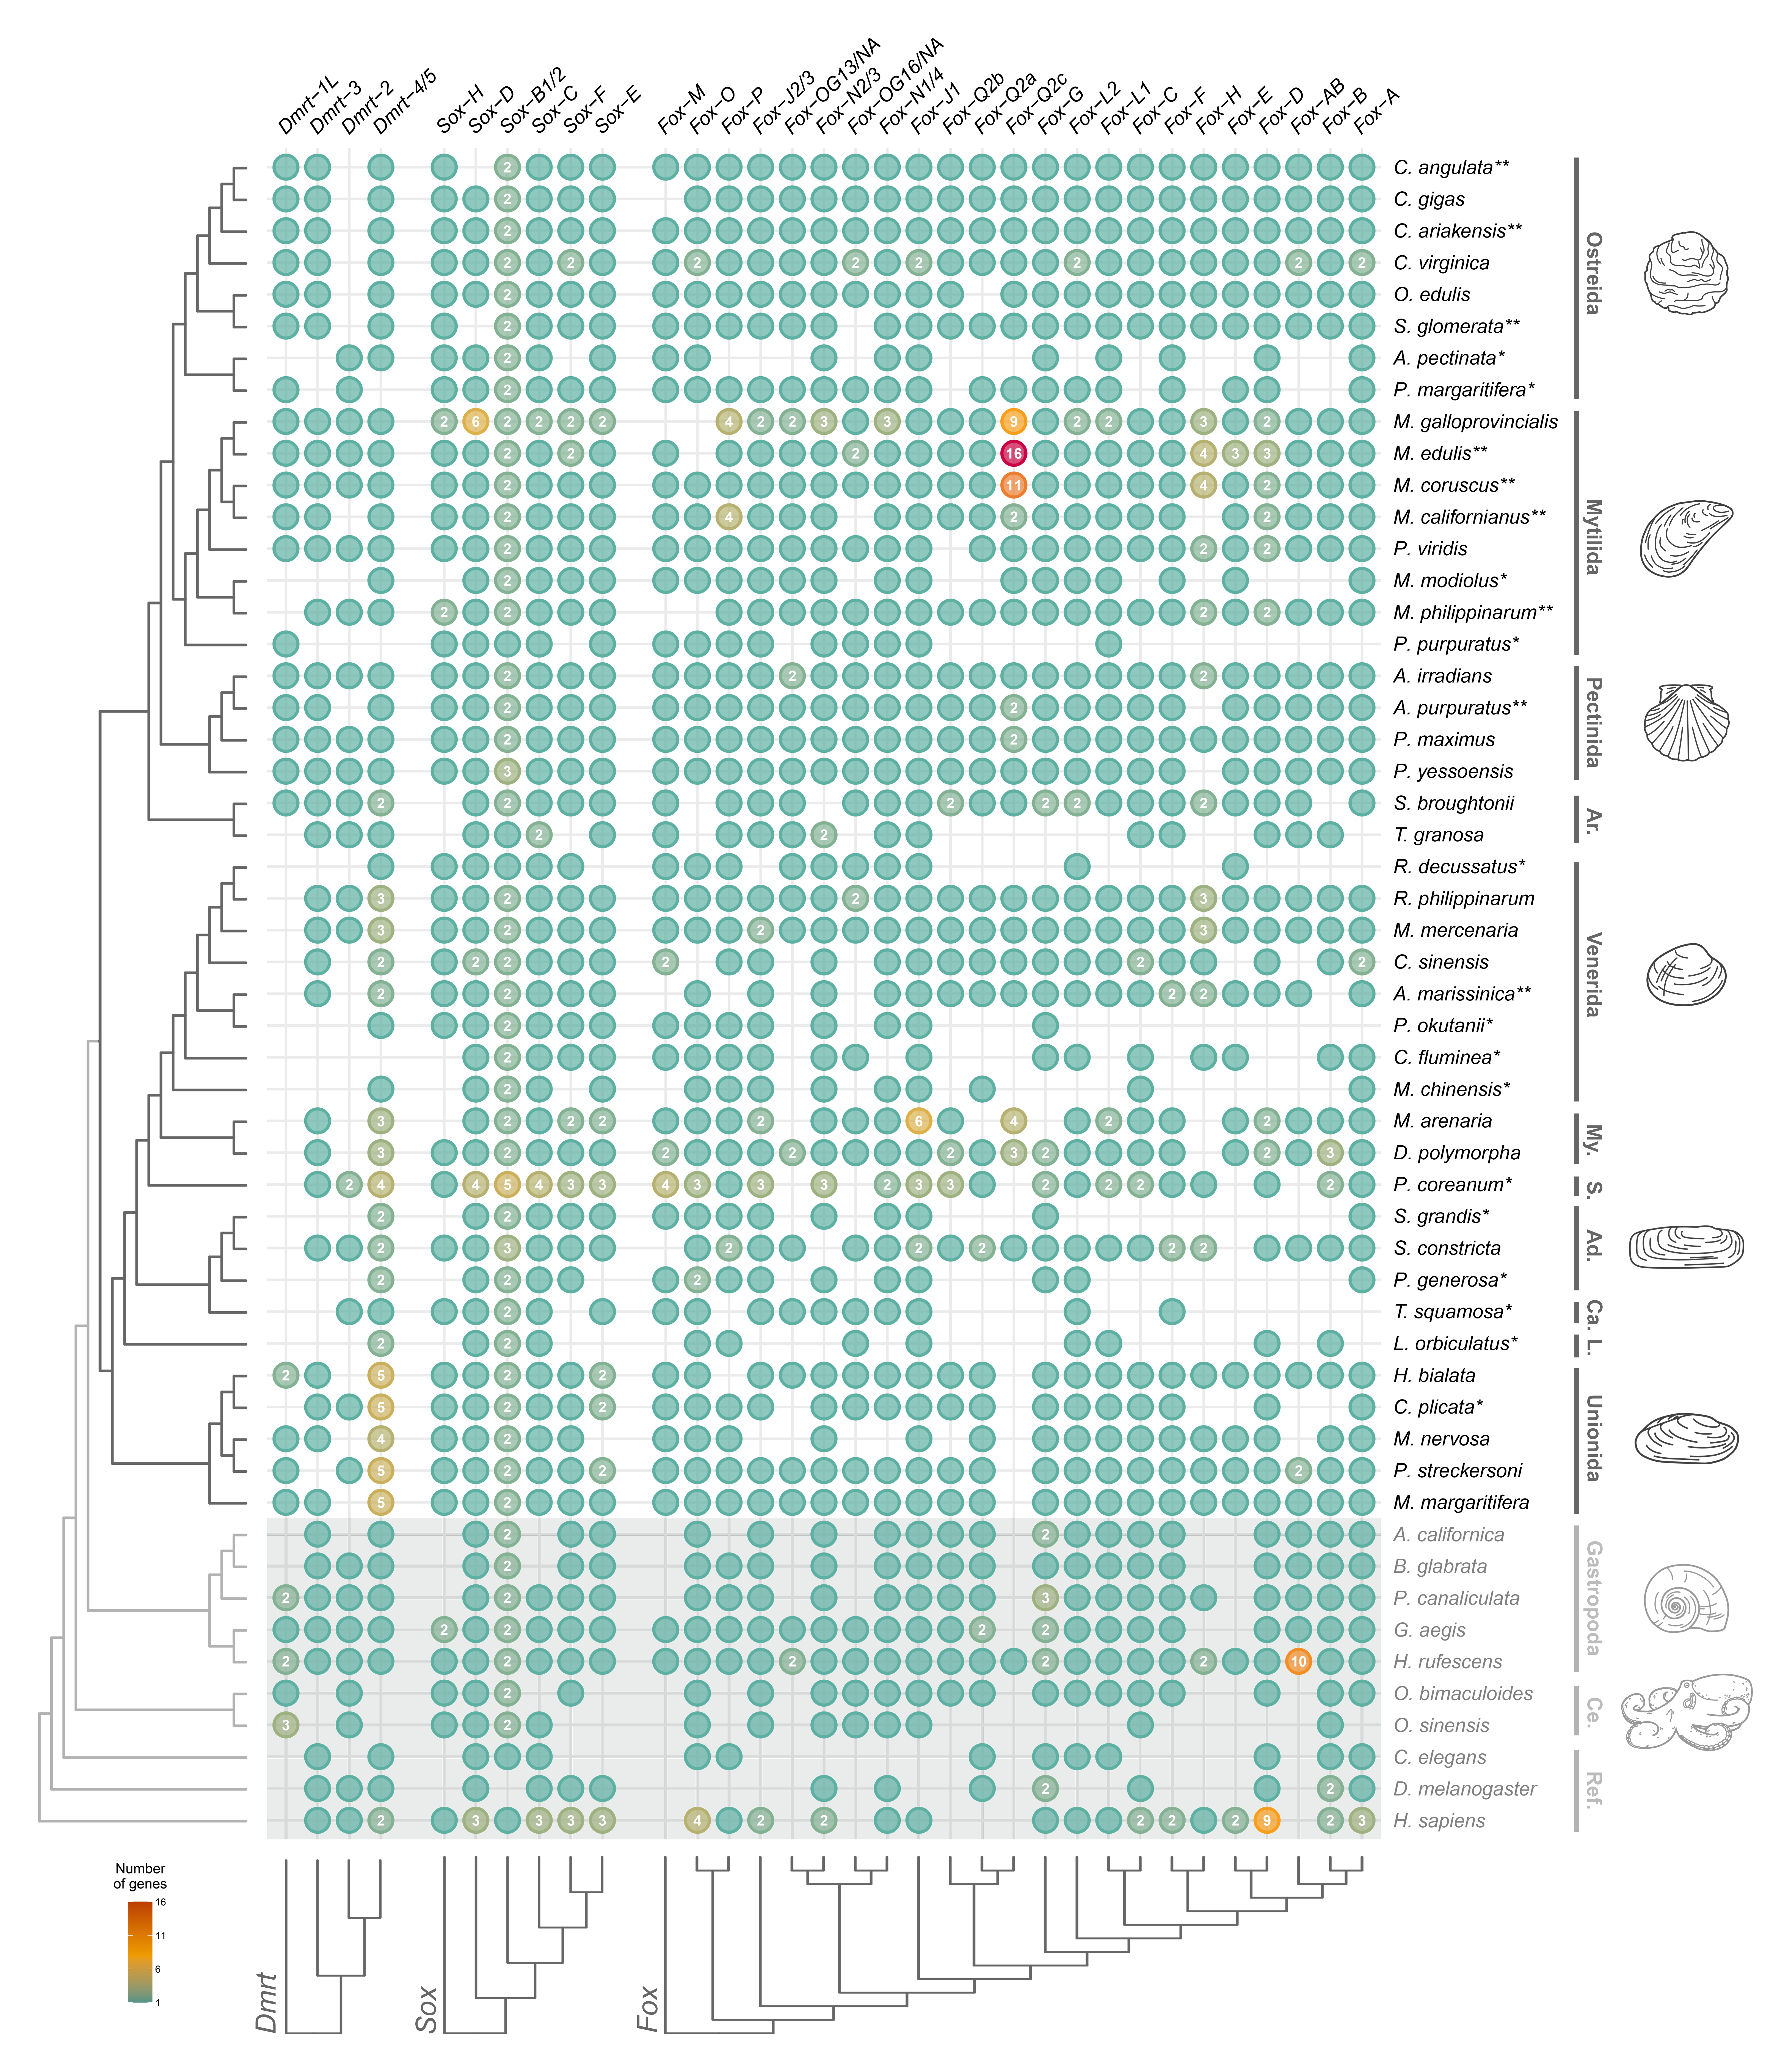
\includegraphics[width=\textwidth]{chapter3/figure_2.png}
	\captionsetup{width=\textwidth}
	\caption{
		\textbf{\gls{dsfg} complement in bivalves and their outgroups.} Presence/absence of genes in various species are indicated by filled circles. Numbers inside each circle specify genes with 2 or more copies. The shaded area highlights non-bivalve species, belonging either to other molluscs or to the references. The phylogenetic tree of analyzed species, as inferred from literature, is shown on the left, while major taxonomic groups are reported on the right. Species represented by transcriptomic data are marked with an asterisk (‘*’), and species not present in the reduced bivalve dataset are marked with two asterisks (‘**’; see main text and \textbf{Fig. \ref{fig:workflow}}); note that the two categories do nor overlap. DSFG trees are shown on the bottom (full trees can be found in \textbf{Supp. Fig. \ref{suppFig:dmrt_bivalves}--\ref{suppFig:fox_bivalves}}). Full species names, along with all assembly and taxonomic information, can be found in \textbf{Supp. Tab. \ref{suppTab:bivalve_dataset}}.  Ad.: Adapedonta; Ar.: Arcida; Ca.: Cardiida; Ce.: Cephalopoda; L.: Lucinida; My.: Myida; Ref.: reference genes; S.: Sphaeriida.
	}
	\label{fig:DSFG_bivalveCompilation}
\end{figure}

\subsection{Amino acid sequence divergence of Dmrt, Sox, and Fox genes in bivalves}
In the reduced bivalve dataset, OrthoFinder collectively analysed $>$1.2G genes distributed in 34 species. 89.4\% of these genes were placed in orthogroups, while 10.6\% were not. The number of retrieved \glspl{sco} is 5, which is drastically low but can be explained considering the mixed nature of the dataset, that is, it includes both genomes and transcriptomes with highly different BUSCO scores (\textbf{Supp. Tab. \ref{suppTab:bivalve_dataset}}). In order to be able to analyse a greater number of genes, we decomposed OrthoFinder orthogroups using DISCO and eventually obtained ~11k \glspl{sco} with at least 50\% of the species. By running the same pipeline on \glspl{dsfg}, we included in the \gls{aasd} analysis 32 \glspl{sco} (\textbf{Fig. \ref{fig:DSFG_bivalveCompilation}}) out of 33 initial Possvm-identified groups (\textit{Fox-H} didn’t meet the species occupancy threshold; \textbf{Fig. \ref{fig:DSFG_bivalveDivergence}}).

\begin{figure}
	\centering
	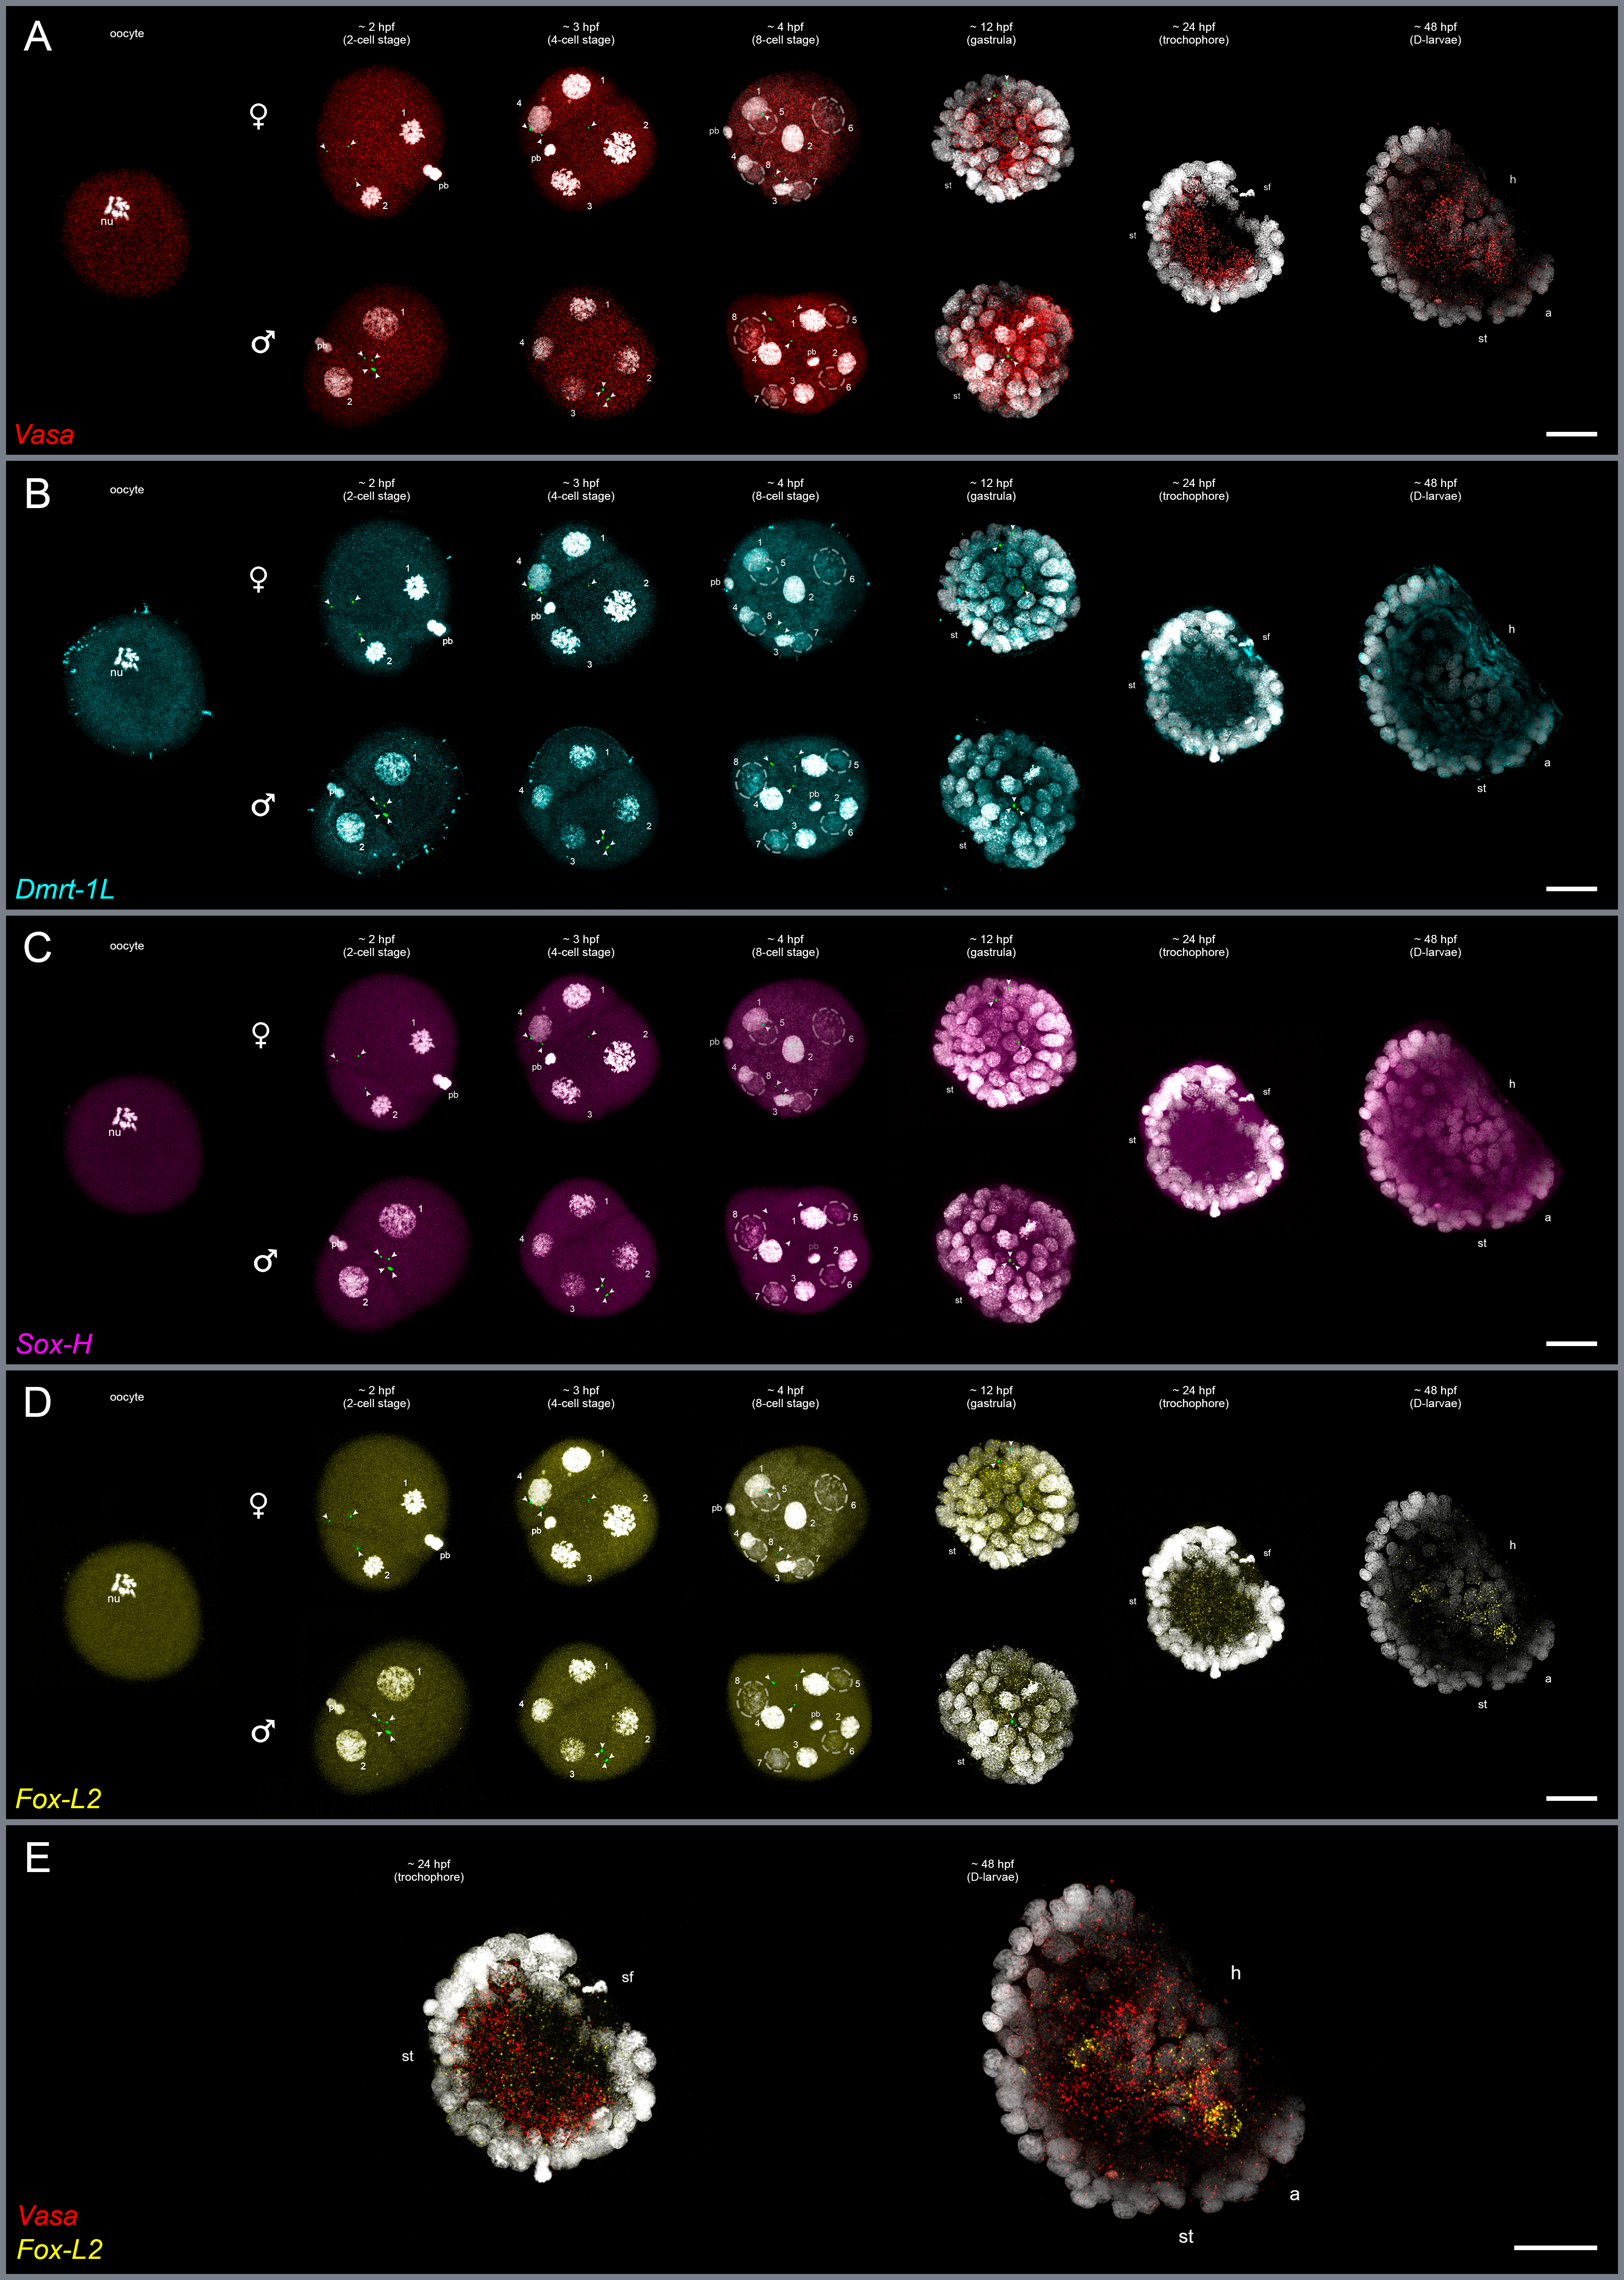
\includegraphics[width=\textwidth]{chapter3/figure_3.png}
	\captionsetup{width=\textwidth}
	\caption{
		\textbf{Distribution of \gls{aasd} of single-copy orthogroups in bivalves (A), including \glspl{dsfg} (B), and their correlations with tip-to-tip distances (C), alignment lengths (D), and number of species (E).} The distribution of AASD has been computed on the median values of pairwise distances of $>$11k \glspl{sco} from the reduced bivalve dataset (see main text and \textbf{Fig. \ref{fig:workflow}}). Genes have been divided according to their median \gls{aasd} value into three different groups, which are indicated by different colors and increasing numbers (Groups 1, 2, and 3). Circle heights of \glspl{dsfg} show the median value of their \gls{aasd}, while the size indicates the number of represented species. \gls{dsfg} trees are shown on the bottom (full trees can be found in \textbf{Supp. Fig. \ref{suppFig:dmrt_bivalves}--\ref{suppFig:fox_bivalves}}). Darker points in C--E indicate \gls{dsfg} \glspl{sco}. The correlation between the amino acid distance and the tip-to-tip distance has been computed on 200 randomly-selected orthogroups.
	}
	\label{fig:DSFG_bivalveDivergence}
\end{figure}

From the distribution of median \gls{aasd}, 112 genes were assigned to Group 1 (1\% upper quantile), 447 to Group 2 (5\% upper quantile), and 10.603 to Group 3. Most of the \glspl{dsfg} (29/32) fell in Group 3 (\textbf{Fig. \ref{fig:DSFG_bivalveDivergence}}), which means they have a median \gls{aasd} comparable to the vast majority of other genes in bivalves (median level of the genomes). Just \gls{dmrt-1l}, \textit{Sox-H}, and \textit{Sox-F} showed higher divergences, and have been accordingly placed in Group 2. Overall, pairwise \gls{aasd} proved to be a good approximation of the tip-to-tip distances ($R = 0.84, p < \num{2.2e-16}$, calculated on 200 randomly-selected trees; \textbf{Fig. \ref{fig:DSFG_bivalveDivergence}C}), while it showed no influence from the alignment length ($R = 0.11$) or the number of represented species ($R = -0.23$; \textbf{Fig. \ref{fig:DSFG_bivalveDivergence}D--E}). Genes from Group 1 and Group 2 are strongly involved in cellular regulatory processes (such as those related to the metabolism of nucleic acids, proteins, and other macromolecules), but also in development and response to external stimuli, as shown by the GO-term enrichment analysis (\textbf{Tab. \ref{tab:enrichedGOs}}; \textbf{Supp. Tab. S10}).

\begin{landscape}
	\footnotesize
	\begin{longtable}{@{}lllccr@{}}
		\caption{\textbf{Enriched GO terms for Group 1 and Group 2 genes of bivalves, mammals, and \textit{Drosophila}.} The extended version of the table, which includes also the expected number of annotated genes per GO term and all the other enriched GO terms, can be accessed in \textbf{Supp. Tab. S10}.}
		\label{tab:enrichedGOs}                                                                                                                                                                                                                                                                                                                                                                                \\
		\toprule
		\multicolumn{1}{c}{\textbf{Dataset}}           & \multicolumn{1}{c}{\textbf{GO.ID}} & \multicolumn{1}{c}{\textbf{Term}}                                         & \textbf{\begin{tabular}[c]{@{}c@{}}Annotated\\ genes\end{tabular}} & \textbf{\begin{tabular}[c]{@{}c@{}}Significant\\ genes\end{tabular}} & \multicolumn{1}{c}{\textbf{\begin{tabular}[c]{@{}c@{}}Corrected\\ p-value\end{tabular}}} \\* \midrule \midrule
		\endfirsthead
		%
		\multicolumn{6}{c}%
		{{\bfseries Tab. \thetable\ continued from previous page}}                                                                                                                                                                                                                                                                                                                                             \\
		\toprule
		\multicolumn{1}{c}{\textbf{Dataset}}           & \multicolumn{1}{c}{\textbf{GO.ID}} & \multicolumn{1}{c}{\textbf{Term}}                                         & \textbf{\begin{tabular}[c]{@{}c@{}}Annotated\\ genes\end{tabular}} & \textbf{\begin{tabular}[c]{@{}c@{}}Significant\\ genes\end{tabular}} & \multicolumn{1}{c}{\textbf{\begin{tabular}[c]{@{}c@{}}Corrected\\ p-value\end{tabular}}} \\* \midrule \midrule
		\endhead
		%
		\endfoot
		%
		\endlastfoot
		%
		\multirow{21}{*}{\textbf{Bivalvia}}            & GO:0060255                         & regulation of macromolecule metabolic process                             & 737                                                                & 59                                                                   & 0.04525                                                                                  \\
		                                               & GO:0080090                         & regulation of primary metabolic process                                   & 673                                                                & 53                                                                   & 0.01818                                                                                  \\
		                                               & GO:0019219                         & regulation of nucleobase-containing compound metabolic process            & 541                                                                & 41                                                                   & 0.02388                                                                                  \\
		                                               & GO:0006351                         & DNA-templated transcription                                               & 571                                                                & 39                                                                   & 0.03767                                                                                  \\
		                                               & GO:0032774                         & RNA biosynthetic process                                                  & 579                                                                & 39                                                                   & 0.04490                                                                                  \\
		                                               & GO:0051252                         & regulation of RNA metabolic process                                       & 517                                                                & 37                                                                   & 0.02719                                                                                  \\
		                                               & GO:0006355                         & regulation of DNA-templated transcription                                 & 490                                                                & 35                                                                   & 0.03751                                                                                  \\
		                                               & GO:2001141                         & regulation of RNA biosynthetic process                                    & 491                                                                & 35                                                                   & 0.03844                                                                                  \\
		                                               & GO:0006950                         & response to stress                                                        & 370                                                                & 33                                                                   & 0.01949                                                                                  \\
		                                               & GO:0032502                         & developmental process                                                     & 261                                                                & 27                                                                   & 0.04445                                                                                  \\
		                                               & GO:0006468                         & protein phosphorylation                                                   & 345                                                                & 23                                                                   & 0.02483                                                                                  \\
		                                               & GO:0031325                         & positive regulation of cellular metabolic process                         & 125                                                                & 17                                                                   & 0.00801                                                                                  \\
		                                               & GO:0010604                         & positive regulation of macromolecule metabolic process                    & 151                                                                & 17                                                                   & 0.04047                                                                                  \\
		                                               & GO:0051172                         & negative regulation of nitrogen compound metabolic process                & 117                                                                & 16                                                                   & 0.00814                                                                                  \\
		                                               & GO:0051173                         & positive regulation of nitrogen compound metabolic process                & 137                                                                & 15                                                                   & 0.02454                                                                                  \\
		                                               & GO:0006310                         & DNA recombination                                                         & 66                                                                 & 14                                                                   & 0.00087                                                                                  \\
		                                               & GO:0048513                         & animal organ development                                                  & 83                                                                 & 12                                                                   & 0.04088                                                                                  \\
		                                               & GO:0010629                         & negative regulation of gene expression                                    & 78                                                                 & 11                                                                   & 0.00048                                                                                  \\
		                                               & GO:0023051                         & regulation of signaling                                                   & 133                                                                & 11                                                                   & 0.02872                                                                                  \\
		                                               & GO:0045934                         & negative regulation of nucleobase-containing compound metabolic process   & 64                                                                 & 11                                                                   & 0.03637                                                                                  \\
		                                               & GO:0009605                         & response to external stimulus                                             & 90                                                                 & 11                                                                   & 0.04544                                                                                  \\
		\multirow{1}{*}{\textbf{Bivalvia}}             & GO:0044419                         & biological process involved in interspecies interaction between organisms & 63                                                                 & 11                                                                   & 0.04761                                                                                  \\* \midrule
		\multirow{22}{*}{\textbf{Mammalia}}            & GO:0006955                         & immune response                                                           & 1297                                                               & 145                                                                  & 0.00061                                                                                  \\
		                                               & GO:0098542                         & defense response to other organism                                        & 853                                                                & 112                                                                  & 0.02066                                                                                  \\
		                                               & GO:0045087                         & innate immune response                                                    & 647                                                                & 82                                                                   & 8.5e-10                                                                                  \\
		                                               & GO:0001817                         & regulation of cytokine production                                         & 630                                                                & 51                                                                   & 0.04660                                                                                  \\
		                                               & GO:0042742                         & defense response to bacterium                                             & 233                                                                & 45                                                                   & 1.7e-07                                                                                  \\
		                                               & GO:0006954                         & inflammatory response                                                     & 642                                                                & 45                                                                   & 0.01735                                                                                  \\
		                                               & GO:0019221                         & cytokine-mediated signaling pathway                                       & 382                                                                & 44                                                                   & 3.9e-07                                                                                  \\
		                                               & GO:0002250                         & adaptive immune response                                                  & 342                                                                & 44                                                                   & 1.3e-05                                                                                  \\
		                                               & GO:0001819                         & positive regulation of cytokine production                                & 402                                                                & 41                                                                   & 0.02723                                                                                  \\
		                                               & GO:0002697                         & regulation of immune effector process                                     & 308                                                                & 37                                                                   & 0.04426                                                                                  \\
		                                               & GO:0042110                         & T cell activation                                                         & 432                                                                & 35                                                                   & 0.02564                                                                                  \\
		                                               & GO:0051607                         & defense response to virus                                                 & 257                                                                & 34                                                                   & 1.9e-07                                                                                  \\
		                                               & GO:0048232                         & male gamete generation                                                    & 491                                                                & 32                                                                   & 0.02255                                                                                  \\
		                                               & GO:0007283                         & spermatogenesis                                                           & 478                                                                & 31                                                                   & 0.02801                                                                                  \\
		                                               & GO:0070661                         & leukocyte proliferation                                                   & 273                                                                & 29                                                                   & 0.01285                                                                                  \\
		                                               & GO:0002449                         & lymphocyte mediated immunity                                              & 221                                                                & 29                                                                   & 0.04833                                                                                  \\
		                                               & GO:0070663                         & regulation of leukocyte proliferation                                     & 212                                                                & 25                                                                   & 0.01870                                                                                  \\
		                                               & GO:0050727                         & regulation of inflammatory response                                       & 300                                                                & 24                                                                   & 0.00235                                                                                  \\
		                                               & GO:0031349                         & positive regulation of defense response                                   & 240                                                                & 24                                                                   & 0.01239                                                                                  \\
		                                               & GO:0002768                         & immune response-regulating cell surface receptor signaling pathway        & 177                                                                & 22                                                                   & 0.00336                                                                                  \\
		                                               & GO:0050829                         & defense response to Gram-negative bacterium                               & 66                                                                 & 17                                                                   & 1.7e-10                                                                                  \\
		                                               & GO:0071222                         & cellular response to lipopolysaccharide                                   & 164                                                                & 17                                                                   & 0.00012                                                                                  \\
		\multirow{13}{*}{\textbf{Mammalia}}            & GO:0010466                         & negative regulation of peptidase activity                                 & 163                                                                & 16                                                                   & 0.00036                                                                                  \\
		                                               & GO:0002429                         & immune response-activating cell surface receptor signaling pathway        & 164                                                                & 16                                                                   & 0.00243                                                                                  \\
		                                               & GO:1903555                         & regulation of tumor necrosis factor superfamily cytokine production       & 137                                                                & 16                                                                   & 0.01244                                                                                  \\
		                                               & GO:0071706                         & tumor necrosis factor superfamily cytokine production                     & 137                                                                & 16                                                                   & 0.01244                                                                                  \\
		                                               & GO:0070665                         & positive regulation of leukocyte proliferation                            & 132                                                                & 16                                                                   & 0.02765                                                                                  \\
		                                               & GO:0045089                         & positive regulation of innate immune response                             & 113                                                                & 16                                                                   & 0.03224                                                                                  \\
		                                               & GO:0071356                         & cellular response to tumor necrosis factor                                & 175                                                                & 15                                                                   & 0.00219                                                                                  \\
		                                               & GO:0002695                         & negative regulation of leukocyte activation                               & 148                                                                & 15                                                                   & 0.01151                                                                                  \\
		                                               & GO:0002456                         & T cell mediated immunity                                                  & 82                                                                 & 15                                                                   & 0.01605                                                                                  \\
		                                               & GO:0002705                         & positive regulation of leukocyte mediated immunity                        & 113                                                                & 15                                                                   & 0.01837                                                                                  \\
		                                               & GO:0032680                         & regulation of tumor necrosis factor production                            & 133                                                                & 15                                                                   & 0.03262                                                                                  \\
		                                               & GO:0032640                         & tumor necrosis factor production                                          & 133                                                                & 15                                                                   & 0.03262                                                                                  \\
		                                               & GO:0050866                         & negative regulation of cell activation                                    & 165                                                                & 15                                                                   & 0.04048                                                                                  \\* \midrule
		\multirow{10}{*}{\textit{\textbf{Drosophila}}} & GO:0000819                         & sister chromatid segregation                                              & 140                                                                & 11                                                                   & 0.02927                                                                                  \\
		                                               & GO:0070192                         & chromosome organization involved in meiotic cell cycle                    & 54                                                                 & 9                                                                    & 0.00849                                                                                  \\
		                                               & GO:0007131                         & reciprocal meiotic recombination                                          & 37                                                                 & 7                                                                    & 0.00066                                                                                  \\
		                                               & GO:0007143                         & female meiotic nuclear division                                           & 54                                                                 & 6                                                                    & 0.02270                                                                                  \\
		                                               & GO:0035967                         & cellular response to topologically incorrect protein                      & 44                                                                 & 5                                                                    & 0.03334                                                                                  \\
		                                               & GO:0035966                         & response to topologically incorrect protein                               & 47                                                                 & 5                                                                    & 0.04266                                                                                  \\
		                                               & GO:0007141                         & male meiosis I                                                            & 13                                                                 & 4                                                                    & 0.00150                                                                                  \\
		                                               & GO:0140543                         & positive regulation of piRNA transcription                                & 3                                                                  & 3                                                                    & 6.9e-05                                                                                  \\
		                                               & GO:0010526                         & retrotransposon silencing                                                 & 8                                                                  & 3                                                                    & 0.00331                                                                                  \\
		                                               & GO:0007130                         & synaptonemal complex assembly                                             & 10                                                                 & 3                                                                    & 0.00666                                                                                  \\
		\multirow{5}{*}{\textit{\textbf{Drosophila}}}  & GO:0030719                         & P granule organization                                                    & 11                                                                 & 3                                                                    & 0.00888                                                                                  \\
		                                               & GO:0071218                         & cellular response to misfolded protein                                    & 12                                                                 & 3                                                                    & 0.01149                                                                                  \\
		                                               & GO:0051788                         & response to misfolded protein                                             & 12                                                                 & 3                                                                    & 0.01149                                                                                  \\
		                                               & GO:0007135                         & meiosis II                                                                & 15                                                                 & 3                                                                    & 0.02169                                                                                  \\
		                                               & GO:0034508                         & centromere complex assembly                                               & 19                                                                 & 3                                                                    & 0.04094                                                                                  \\* \bottomrule \bottomrule
	\end{longtable}
\end{landscape}

\subsection{Dmrt, Sox, and Fox genes, and amino acid sequence divergence in the test datasets}
The \gls{dsfg} datasets retrieved in mammals and fruit flies are far more complete than those in bivalves, and most of the already-recognised orthology groups have been identified.

In mammals, we retrieved 7 \gls{dmrt} orthology groups with about 3.1\% of missing data, 20 \gls{sox} orthology groups with about 8.1\% of missing data, and 42 \gls{fox} orthology groups with about 4.6\% of missing data (\textbf{Supp. Fig. \ref{suppFig:DSFG_testCompilation}A, \ref{suppFig:dmrt_mammals}--\ref{suppFig:fox_mammals}}; \textbf{Supp. Tab. S8}). Of these, just \textit{Sox-5} was not included in the subsequent \gls{aasd} analysis, as it did not meet the 50\%-species occupancy threshold. OrthoFinder analysed about 650M genes, and the number of \glspl{sco} used in the \gls{aasd} analysis (thus resulting from the DISCO-based orthogroup decomposition pipeline) is $>$16k (\textbf{Fig. \ref{fig:DSFG_testDivergence}A}). From the distribution of median \gls{aasd}, 163 genes were assigned to Group 1, 649 to Group 2, and 15.355 to Group 3. Most of the \glspl{dsfg} (66/68) fell in Group 3 (\textbf{Fig. \ref{fig:DSFG_testDivergence}B}), while \gls{sry} and \textit{Fox-D4} showed higher divergences, and have been accordingly placed in Group 1 and 2, respectively. Genes from Group 1 and Group 2 show a strong enrichment in immune-related functions (such as innate and adaptive immune response, defence response to bacteria and viruses, lymphocyte methabolism, etc.), but also in reproductive processes (such as spermatogenesis; \textbf{Tab. \ref{tab:enrichedGOs}}; \textbf{Supp. Tab. S10}).

Concerning \textit{Drosophila}, we retrieved 4 \gls{dmrt} orthology groups with about 1.7\% of missing data, 7 \gls{sox} orthology groups with about 3.9\% of missing data, and 17 \gls{fox} genes with about 8.3\% of missing data (\textbf{Supp. Fig. \ref{suppFig:DSFG_testCompilation}B, \ref{suppFig:dmrt_drosophila}--\ref{suppFig:fox_drosophila}}; \textbf{Supp. Tab. S9}). OrthoFinder analysed about 240M, and the distribution of median \gls{aasd} was built after $>$12k \glspl{sco} (\textbf{Fig. \ref{fig:DSFG_testDivergence}C}). 126 genes were assigned to Group 1, 501 to Group 2, and 11.880 to Group 3. All of the \glspl{dsfg} have been used in the \gls{aasd} analysis, but none of them have been placed in Group 1 or 2, that is, all the \glspl{dsfg} in \textit{Drosophila} have an \gls{aasd} comparable to the median level of the genome (\textbf{Fig. \ref{fig:DSFG_testDivergence}D}). Genes of Group 1 and Group 2 show a GO-term enrichment in meiotic processes, such as chromosome/chromatid organisation, and retrotransposon silencing (\textbf{Tab. \ref{tab:enrichedGOs}}; \textbf{Supp. Tab. S10}).

\begin{figure}
	\centering
	\includegraphics[width=0.9\textwidth]{chapter3/figure_4.png}
	\captionsetup{width=\textwidth}
	\caption{
		\textbf{Distribution of amino acid divergence (AASD) of single-copy orthogroups in Mammalia (A) and \textit{Drosophila} (C), including Dmrt, Sox, and Fox genes (DSFGs; B-D).} The distributions of AASD in mammals and fruit flies have been computed on the median values of pairwise distances of over 16k and 12k SCOs, respectively. Genes have been divided according to their median AASD value into three different groups, which are indicated by different colors and increasing numbers (Groups 1, 2, and 3). Circle heights of DSFGs show the median value of their AASD, while the size indicates the number of represented species. DSFG trees are shown on the bottom (full trees can be found in \textbf{Supp. Fig. \ref{suppFig:dmrt_mammals}--\ref{suppFig:fox_mammals}} for mammals and in \textbf{Supp. Fig. \ref{suppFig:dmrt_drosophila}--\ref{suppFig:fox_drosophila}} for fruit flies). Insets: scheme of the sex-determination molecular pathways in \textit{Mus musculus} and in \textit{Drosophila melanogaster}, with shown the main genes involved (adapted from \textbf{\cite{beukeboom2014evolution}}). Green arrows indicate transcription activations, red arrows indicate transcription suppressions. X: sex chromosomes; A: autosomal chromosomes; \textit{DSX\textsuperscript{M/F}}: \textit{DSX} splicing variants present in males or females, respectively.
	}
	\label{fig:DSFG_testDivergence}
\end{figure}

\section{Discussion} \label{chpater3_discussion}
\subsection{A new manually-curated and phylogenetic-based reference dataset of Dmrt, Sox, and Fox genes in bivalves}
The annotation and characterisation process of a gene family in a certain clade of organisms may harbour many overlooked challenges (\textbf{\cite{vizueta2020bitacora}}). For example, the presence of highly-conserved catalytic domains may hamper the correct identification of the components of a gene family because of insufficient phylogenetic signal, as it is the case for Hox and ParaHox genes and their homeobox motif (\textbf{\cite{baldwin2018new, nicolini2023comparative}}). Conversely, the components of dynamic gene families characterised by abrupt and sequential duplication events may be difficult to sort into separate groups. As a matter of fact, varying levels of sequence heterogeneity and gene copy numbers makes the inference of orthologous groups hard, as for certain clans of the P450 gene family (\textbf{\cite{dermauw2020diversity}}). Regardless of the causes, having a solid and wide phylogenetic context in which to study gene duplications and losses, and orthology relationships, is crucial to overcome these difficulties. In the same way, manual curation and visual inspection of multiple sequence alignments, phylogenetic trees, and gene structures (in terms of domain annotation, start and stop codons, and other feature representations) is helpful, despite being time-demanding and possibly low reproducible. In this study, we characterised the full complement of \glspl{dsfg} in the vast class of bivalves, by leveraging sequence domain annotation, phylogenetics, and manual curation of the dataset. Our aim was to obtain the most reliable gene complements as possible, combined with a vast taxonomic dataset, a solid phylogenetic inference, an openly-available dataset of gene sequences, and a reproducible pipeline for the annotation of gene identity. By doing so, we want to provide a reliable resource for future studies of \glspl{dsfg}, either focused on bivalves or generally in Metazoa.

Concerning the \gls{dmrt} gene family, we identified orthologs of the vertebrate \textit{Dmrt-2}, \textit{Dmrt-3}, and \textit{Dmrt-4/5} (or \textit{A1/A2}; \textbf{\ref{fig:DSFG_bivalveCompilation}; Supp. Fig. \ref{suppFig:dmrt_bivalves}; Supp. Tab. \ref{suppTab:dsfg_bivalveAnnotation}}), which are also expected to have been present in the Bilateria common ancestor (\textbf{\cite{mawaribuchi2019independent}}). \textbf{\cite{wang2023genome}} found that \textit{Dmrt-4/5} is duplicated in \gls{mmer} and \gls{csin} (Venerida), and in \gls{dpol} (Myida), and we confirm this result by tracing back the duplication event to the split between Palaeoheterdonta (here represented by Unionida) and Heterodonta (here represented by Venerida, Myida, Sphaeriida, Adapedonta, Cardiida, and Lucinida; \textbf{Fig. \ref{fig:DSFG_bivalveCompilation}}). Furthermore, we confirm \gls{dmrt-1l} to be present in many bivalve species (mainly belonging to the Ostreida, Pectinida, Mytilida, and Unionida orders; \textbf{Fig. \ref{fig:DSFG_bivalveCompilation}}), as well as in gastropods and \textit{Octopus}. Though, our phylogenetic analysis did not retrieve any unambiguous orthology relationship among \gls{dmrt-1l} and either vertebrate \textit{Dmrt-1} or \textit{Drosophila} \gls{dsx} genes, as instead it was proposed in previous works (\textbf{\cite{li2018foxl2,evensen2022comparative}}). As a matter of fact, the amino acid sequence of the \gls{dmrt-1l} \gls{dm} domain does not recall that of any other \gls{dmrt} gene. Furthermore, it must be considered that various phylogenetic analyses have recovered both \textit{Dmrt-1} and \gls{dsx} genes to be restricted to vertebrates and arthropods, respectively (\textbf{\cite{wexler2014pan,mawaribuchi2019independent,panara2019phylogenetic}}), that is, they do not have any direct ortholog outside their relative clades. Thus, if \gls{dmrt-1l}, \gls{dsx}, and \textit{Dmrt-1} are true orthologs, their origin would need to be placed at least in the Bilateria common ancestor, which seems however to be not the case. All considered, we thus confirm that \gls{dmrt-1l} is not orthologous to \textit{Dmrt-1} and \gls{dsx} and is rather a mollusc-specific gene (\textbf{\cite{evensen2022comparative}}). The monophyly of the group is not supported by the phylogenetic tree inferred with \gls{dmrt} genes from molluscs and the reference species (\textbf{Supp. Fig. \ref
	{suppFig:dmrt_bivalves}}); though, it is recovered when analysing just genes from mollusc species (\textbf{Supp Fig. \ref{suppFig:dmrt_molluscOnly}}). To this regard, we speculate that in our analysis, the difficulty in obtaining the monophyly of \gls{dmrt-1l} genes may have arisen primarily because of the many \gls{cele}-restricted genes (\textbf{Supp. Tab. \ref{suppTab:reference_dsfgs}}), which are placed among the other bivalve genes (\textbf{Supp. Fig. \ref
	{suppFig:dmrt_bivalves}}), but also because of the high \gls{aasd} of \gls{dmrt-1l} genes (see the following section), which hampers a straight-forward phylogenetic reconstruction. Furthermore, our broad-context analysis allowed us to identify some cases of incorrect gene identification in bivalves, which have arisen because of erroneous or ambiguous annotations in previous works, as a result of limited datasets or analyses. For example, (i) the scallop-specific cluster of \gls{dmrt} genes retrieved by \textbf{\cite{wang2023genome}} rather belongs to the \gls{dmrt-1l} group, and (ii) the classification of \gls{dmrt} genes in Crassostrea species provided by \textbf{\cite{zeng2024genome}} needs to be revised following the one of this work: \textit{Dmrt-1} genes are \textit{Dmrt-4/5}; \textit{Dmrt-2} genes are \textit{Dmrt-3}; \textit{Dmrt-3} genes are \gls{dmrt-1l}; hence, \textit{Crassostrea} species do not have \textit{Dmrt-2} genes.

For what concerns the \gls{sox} gene family, bivalves (or molluscs) do not show any major clade-restricted gene, as only the five Bilateria-specific \gls{sox} groups (\textit{Sox-B1/2}, \textit{Sox-C}, \textit{Sox-D}, \textit{Sox-E}, and \textit{Sox-F}) and \textit{Sox-H} have been identified (\textbf{Fig. \ref{fig:DSFG_bivalveCompilation}; Supp. Fig. \ref{suppFig:sox_bivalves}; Supp. Tab. \ref{suppTab:dsfg_bivalveAnnotation}}), in accordance with previous findings (\textbf{\cite{yu2017genome,evensen2022comparative, wang2024genome}}). \textit{Sox-B1/2} is clearly made up of two subgroups (i.e., \textit{Sox-B1} and \textit{Sox-B2}), as expected, but their respective identity could not be unambiguously established, as \textit{Sox-B1/2} genes of reference species do not form separate clusters (\textbf{Supp. Fig. \ref{suppFig:sox_bivalves}}). Even when inferring the phylogenetic tree only of components of the \textit{Sox-B1/2} group from molluscs and reference species, the identity can not be properly established (\textbf{Supp. Fig. \ref{suppFig:sox_B12}}).

Compared to \gls{dmrt} and \gls{sox} genes, the \gls{fox} gene family appears as the most dynamic in terms of gene presence/absence, as already shown by other works (\textbf{\cite{wu2020identification, seudre2022fox, schomburg2022phylogenetic}}). Our phylogenetic analysis successfully recovered Group I and Group II of \gls{fox} genes (\textbf{\cite{larroux2008genesis}}), which include the four \gls{fox} genes that were present in the Bilateria common ancestor (\textit{Fox-C}, \textit{Fox-F}, \textit{Fox-L1}, and \textit{Fox-Q1}; \textbf{Fig. \ref{fig:DSFG_bivalveCompilation}; Supp. Fig. \ref{suppFig:fox_bivalves}; Supp. Tab. \ref{suppTab:dsfg_bivalveAnnotation}; \cite{shimeld2010clustered}}). To our knowledge, this is the first broad-taxonomic identification and classification of \gls{fox} genes in bivalves, as up to now they have been systematically characterised only in \gls{cgig} (\textbf{\cite{yang2014phylogeny}}), \gls{pyes} (now \textit{Mizuhopecten yessoensis}; \textbf{\cite{wu2020identification}}), and \gls{rphi} (\textbf{\cite{liu2024characterization}}). Firstly, our analysis confirms the absence in molluscs of \textit{Fox-I}, \textit{Fox-Q1}, \textit{Fox-R}, \textit{Fox-S} (\textbf{Supp. Fig. \ref{suppFig:fox_bivalves}}), which are in fact thought to have emerged with the diversification of deuterostomes or vertebrates (\textbf{\cite{yang2014phylogeny, wu2020identification, seudre2022fox, schomburg2022phylogenetic}}). Furthermore, we have found many \gls{fox} groups that appeared as mollusc-specific and/or still-unnamed at a first analysis. However, a more in-depth investigation revealed a different scenario. \textit{Fox-OG2/NA} appears close to the human \textit{Fox-M} gene in the phylogenetic tree, but they do not form a monophyletic group (\textbf{Supp. Fig. \ref{suppFig:fox_bivalves}}). However, by comparing \textit{Fox-OG2/NA} sequences and phylogenetic tree with those analysed by \textbf{\cite{yang2014phylogeny}}, \textbf{\cite{wu2020identification}}, \textbf{\cite{schomburg2022phylogenetic}}, and \textbf{\cite{seudre2022fox}}, it appears clear that this group of \gls{fox} genes is indeed \textbf{Fox-M}. However, our analysis has failed to retrieve a monophyletic relationship among bivalve and human \textit{Fox-M} genes, even when inferring a tree with just \textit{Fox-J2}, \textit{Fox-M}, \textit{Fox-O}, and \textit{Fox-P} complements (\textbf{Supp. Fig. \ref{suppFig:fox_JMOP}}), which belong to the same \gls{fox} group. Regarding the \textit{Fox-OG39/NA} group, it does not have any homolog in reference species (\textbf{Supp. Fig. \ref{suppFig:fox_bivalves}}) but is found to belong to the \textit{Fox-AB} group by sequence comparison with previous works (\textbf{\cite{yang2014phylogeny, wu2020identification, seudre2022fox}}). \textit{Fox-AB} was formerly described only in the sea urchin \gls{spur} and the lancelet \gls{bflo} (\textbf{\cite{tu2006sea,yu2008fox}}), but was later identified also in several Spiralia lineages, including molluscs (e.g., \textbf{\cite{yang2014phylogeny, wu2020identification, seudre2022fox}}). A similar situation concerns \textit{Fox-OG15/NA} and \textit{Fox-OG28/NA}, which again could not be named based on orthology relationships with the reference species genes (\textbf{Supp. Fig. \ref{suppFig:fox_bivalves}}), but actually represent two lineage-specific expansions of the \textit{Fox-Q2} group (named \textit{Fox-Q2b} and \textit{Fox-Q2c}), as already appointed in previous studies (\textbf{\cite{yang2014phylogeny, wu2020identification}}). This observation fits within the wider context of the \textit{Fox-Q2} group expansion in Bilateria and, particularly, in Spiralia, that led to remarkable differences in their gene copy numbers across various clades (\textbf{\cite{seudre2022fox}}). Two additional \gls{fox} genes have been previously identified in bivalves, and were named \textit{Sox-Y} and \textit{Sox-Z} (\textbf{\cite{yang2014phylogeny, wu2020identification}}). In our analysis, these \gls{fox} groups were identified as \textit{Fox-OG13/NA} and \textit{Fox-OG16/NA}, after sequence comparison of \gls{fox} genes from \gls{cgig} and \gls{pyes}. On one hand, \textit{Fox-Y} was firstly identified in \gls{spur} (\textbf{\cite{tu2006sea}}) and only recently in a few bivalve species (\textbf{\cite{yang2014phylogeny, wu2020identification}}). However, when analysing bivalve and \gls{spur} \gls{fox} genes, we failed in retrieving such a clear orthology relationship, as \gls{spur} \textit{Fox-Y} does not fall within the phylogenetic range of bivalve \textit{Fox-OG13/NA}, which contains the supposed \textit{Fox-Y} orthologs (\textbf{Supp. Fig. \ref{suppFig:fox_spur}}). Also, the forkhead domains of \textit{Fox-OG13/NA} genes were annotated as ‘forkhead domain P’ (\textbf{Supp. Tab \ref{suppTab:dsfg_bivalveAnnotation}}). On the other hand, \textit{Fox-Z} was firstly identified in bivalves and in several other protostomes, thanks to a phylogenetic work including the brachiopod \gls{lung}, the annelid \gls{ctel}, the scorpion \gls{cscu}, and the centipede \gls{smar} (\textbf{\cite{wu2020identification}}). However, later works have not recovered this \gls{fox} gene, even when analysing annelids (\textbf{\cite{seudre2022fox}}) and panarthropods (\textbf{\cite{schomburg2022phylogenetic}}) in a more focused effort. In this case, the forkhead domains were annotated as either a generic ‘forkhead domain’ or a ‘forkhead domain Q2’ (\textbf{Supp. Tab. \ref{suppTab:dsfg_bivalveAnnotation}}). All considered, we argue that bivalves possess two additional \gls{fox} groups (here \textit{Fox-OG13/NA} and \textit{Fox-OG16/NA}; \textbf{Fig. \ref{fig:DSFG_bivalveCompilation}; Supp. Fig. \ref{suppFig:fox_bivalves}; Supp. Tab. \ref{suppTab:dsfg_bivalveAnnotation}}) which are shared with other mollusc species, as revealed also by other authors. However, given the discordant results of the phylogenetic hypothesis and domain annotation, we think that a more thorough investigation on their orthology relationships with \gls{fox} genes from other Metazoa is needed, and thus we chose to not employ their former names \textit{Fox-Y} and \textit{Fox-Z}.

Besides the \gls{dsfg} groups discussed so far, it must be also considered that many orphan genes have been identified (\textbf{Supp. Fig. \ref{suppFig:dmrt_bivalves}--\ref{suppFig:fox_bivalves}; Supp. Tab. \ref{suppTab:dsfg_bivalveAnnotation}}). For example, \textbf{\cite{wu2020identification}} identified a duplication event of \textit{Fox-H} genes in \gls{cgig}, which has been recovered also in our analysis for the entire Ostreida clade (\textit{Fox-OG36/NA}; \textbf{Supp. Fig. \ref{suppFig:fox_bivalves}}). Similarly, a gene orthology group putatively specific to Pteriomorphia has been identified among \gls{sox} genes (\textit{Sox-OG1/NA}). Of course, these genes deserve as much attention as their widely-distributed paralogs, as they may constitute true group-specific expansions and may play fundamental roles in some biological processes. However, they have not been discussed here or included in \textbf{Fig. \ref{fig:DSFG_bivalveCompilation}} for clarity purposes, but they are freely available in supplementary materials.

Overall, our analysis clearly shows the importance of adopting a wide-angle approach when characterising the members of a gene family, especially for large ones such as the \gls{fox} genes (\textbf{\cite{schomburg2022phylogenetic}}). As a matter of fact, the presence of duplication events and orphan genes needs to be addressed with a broad taxonomic dataset, in order to account for possible mis-annotations, gene phylogenetic mis-placements, and sequence heterogeneity. Additionally, many reference species need to be included for the gene identification process, in order to consider distantly-related genes and obtain a solid annotation. Our gene annotation pipeline also resulted to be very solid, even with non-model organisms and sub-optimal genomic and transcriptomic resources as they are those of bivalves. As a matter of fact, by running the same pipeline on two additional datasets composed of mammal and fruit fly genomes, we were able to obtain high-quality orthology groups in accordance with previous knowledge on the clades (\textbf{Supp. Fig. \ref{suppFig:dmrt_mammals}--\ref{suppFig:fox_drosophila}; Supp. Tab. S8--S9}), with little or no manual curation. Furthermore, this represents also the first broad analysis of \glspl{dsfg} in both mammals and fruit flies, as so far attention has been mainly dedicated to single well-studied organisms or little clades (e.g., \textbf{\cite{jackson2010update}}).

\subsection{High amino acid sequence divergence identifies putative sex-determining genes}
Sex-biased genes tend to evolve more rapidly than unbiased genes at the level of their protein sequences. Accelerated rates have been observed in both male-biased genes (reviewed in \textbf{\cite{parsch2013evolutionary,grath2016sex}}) and female-biased genes (e.g., \textbf{\cite{papa2017anopheles, ghiselli2018comparative}}), but also in \glspl{srg} and primary \glspl{sdg} (\textbf{\cite{oNeil1992drosophila_tra, whitfield1993rapid, deBono1996evolution}}). For example, it has been shown that \gls{dmw}, \gls{dmy}, and \gls{sry} (which are \glspl{sdg} in the African clawed frog \gls{xlae}, in the medaka fish \gls{olat}, and in eutherians, respectively) all have higher substitution rates than their paralogues (\textit{Dmrt-1} for \gls{dmw} and \gls{dmy}, \textit{Sox-3} for \gls{sry}), particularly when considering their DNA-binding domains (\textbf{\cite{mawaribuchi2012molecular}}). Similarly, both a burst of positive selection and a relaxation of purifying selection has been detected in \textit{Drosophila} \gls{sxl} in correspondence with its recruitment at the top of the sex-determing cascade. The same signs of relaxed purifying selection have been found in the downstream targets of \gls{sxl}, that is, \gls{tra} and \gls{dsx}, despite no evidence of positive selection has been detected (\textbf{\cite{mullon2012drosophila_sxl}}).

Considering these shared features of \glspl{srg} and \glspl{sdg}, we decided to look for signs of accelerated sequence evolution in \glspl{dsfg} of bivalves, in order to evaluate if any of them could be \textit{a-priori} associated with \gls{sd} by employing the tools of molecular evolution. However, we wanted to analyse patterns of sequence evolution not only among putative \glspl{srg} and their close paralogs, but also considering the genomic context in which these genes evolve. In fact, our aim was to check whether higher rates of sequence evolution of \glspl{srg} hold true also when compared to other genes not involved in \gls{sd} and not belonging to the same gene family. To do so, we obtained the \gls{aasd} median values of more than 11k \glspl{sco} from bivalve genomes (\textbf{Fig. \ref{fig:DSFG_bivalveDivergence}A}), in order to build a statistical distribution to be used as a reference: if \glspl{srg}/\glspl{sdg} (in this case, \glspl{dsfg}) truly evolve faster than other genes, we may expect them to fall within the 5\% (or even 1\%) upper quantile of the distribution (\textbf{Fig. \ref{fig:DSFG_bivalveDivergence}B}), i.e., within highly divergent genes (Group 1 and Group 2 genes of the distribution; see \textbf{Section \ref{chapter3_MM}}). We chose to use the \gls{aasd} as a metric of sequence evolution (instead of the tip-to-tip distances of phylogenetic trees, which account for more comprehensive evolutionary models) in order to save computational time. As a matter of fact, the \gls{aasd} median values proved to be a good approximation of the tip-to-tip median distances in 200 randomly-selected genes (\textbf{Fig. \ref{fig:DSFG_bivalveDivergence}C}; $R = 0.84, p < \num{2.2e-6}$).

Among \glspl{dsfg}, three fell within the 5\% upper quantile, namely \gls{dmrt-1l}, \textit{Sox-H}, and \textit{Sox-F}. Interestingly, \gls{dmrt-1l} and \textit{Sox-H} have been already proposed to be involved in the male \gls{sd} pathway of \gls{cgig} (\textbf{\textit{inset}} in \textbf{Fig. \ref{fig:DSFG_bivalveDivergence}B}; \textbf{\cite{zhang2014genomic}}), on the basis of \gls{dge} analyses. Specifically, \textit{Sox-H} would play a major role in \gls{cgig} \gls{sd}, by interacting with \gls{dmrt-1l} and determining the onset of the male phenotype development; at the same time, both \textit{Sox-H} and \gls{dmrt-1l} would inhibit \textit{Fox-L2}, which instead is necessary to start the female phenotype development. \gls{dmrt-1l} and \textit{Sox-H} have been appointed several other times to be involved in male-gonad development and differentiation, through \gls{dge} (e.g., \textbf{\cite{teaniniuraitemoana2014gonad, capt2018deciphering, afonso2019gonad}}), \gls{ish} (e.g., \textbf{\cite{naimi2009molecular,li2018foxl2, yue2021variance, liang2019sox2}}) and \gls{rnai} (\textbf{\cite{liang2019sox2, sun2022examination}}). Therefore, the high \gls{aasd} of \gls{dmrt-1l} and \textit{Sox-H} is coherent with previous works, strengthening their role as putative \glspl{srg}.

The relationship between high gene \gls{aasd} and the involvement in SD is particularly enforced when looking at the patterns of \gls{aasd} in the test datasets, which corroborates the solidity of our analysis: (i) from one side, in the mammal dataset—which represents a strictly genetic \gls{sd} system, thus with a master and rapidly-evolving \gls{sdg}, one of the genes from the 5\% upper quantile of the distribution is \gls{sry} (\textbf{Fig. \ref{fig:DSFG_testDivergence}A--B}), the male sex-determining gene in eutherians (\textbf{\textit{inset}} in \textbf{Fig. \ref{fig:DSFG_testDivergence}A--B}); (ii) from the other side, in the fruit fly dataset—which represents a chromosomic \gls{sd} system, thus without any expected difference in the rates of sequence evolution among \glspl{srg}, none of the \gls{dsfg} exhibit significantly high \gls{aasd} (\textbf{Fig. \ref{fig:DSFG_testDivergence}C--D}), including the downstream effector \gls{dsx} (\textit{\textbf{inset}} in \textbf{Fig. \ref{fig:DSFG_testDivergence}D}). Also \gls{sxl} and \gls{tra}, both involved in the \gls{sd} pathway of \textit{Drosophila} (\textit{\textbf{inset}} in \textbf{Fig. \ref{fig:DSFG_testDivergence}D}) do not belong to the group of highly-divergent genes, as they have a mean amino acid divergence of about 0.09 and 0.9, respectively (\textbf{Fig. \ref{fig:DSFG_testDivergence}D}). Therefore, it can be argued that both \gls{dmrt-1l} and \textit{Sox-H} may not only be \glspl{srg}, but may participate in bivalve \gls{sd} as primary \glspl{sdg}, which is reflected in their high \gls{aasd}, as it is observed for \gls{sry} in mammals. As a matter of fact, if they were involved in \gls{sd} just as intermediate actors of the signalling cascade, then we should have not observed a high \gls{aasd}, as \textit{Drosophila} \gls{sxl}, \gls{tra}, and \gls{dsx} seem to suggest. Overall, these patterns of molecular evolution concerning \glspl{srg} and \gls{sdg} are also supported by the way \gls{sd} regulatory networks evolve. As a matter of fact, it has been proposed that the sex-determining cascades tend to arise and be established with a bottom-up mechanism (\textbf{\cite{wilkins1995moving, mullon2012drosophila_sxl, beukeboom2014evolution, capel2017vertebrate}}). This means that the regulative relationships among genes at the bottom of the cascade are settled up prior to the regulative relationships among genes at the top and, consequently, upstream regulators are progressively recruited to fine-tune diverse \gls{sd} signals. These evolutionary patterns eventually produce gene-regulatory networks in which the divergence of the upstream triggers is higher than that of downstream effectors, in terms of both identity and sequence composition (\textbf{\cite{beukeboom2014evolution}}). This mechanism has been proposed for both \textit{Drosophila} (\textbf{\cite{mullon2012drosophila_sxl}}) and vertebrates, despite in the latter case it has been questioned several times (reviewed in \textbf{\cite{capel2017vertebrate}}).

At this point, two main objections can be moved against our approach: (1) the distribution of \gls{aasd} is not appropriate for this kind of inference, as it does not represent the true gene evolutionary (or substitution) rates (which instead are those usually employed when dealing with \glspl{srg} and \glspl{sdg}); (2) the three datasets are not comparable one to each other, as they take into consideration very different animal groups, with different taxonomic rankings and different divergence times (thus, the patterns of \gls{aasd} are the products of other confounding factors not directly related to \gls{sd}). Concerning the first objection, we are aware that the \gls{aasd} does not represent the evolutionary rate itself, but rather its product. However, the two features are tightly linked, as on the long term highly-divergent proteins tend to be produced by genes with high evolutionary (or substitution) rates (\textbf{\cite{echave2016causes}}). By performing a \gls{go}-term enrichment, it emerged that highly-divergent genes of the mammal dataset are mainly involved in the immune response and male spermatogenesis (\textbf{Tab. \ref{tab:enrichedGOs}; Supp. Tab. S10}), which are two processes notoriously connected with rapid sequence evolution (i.e., higher evolutionary rates; \textbf{\cite{swanson2002rapid, murat2023molecular, vinkler2023understanding}}). Similarly, highly-divergent genes from the fruit fly dataset show an enrichment for \gls{go}-terms associated with meiotic-related functions (such as the formation of the synaptonemal complex by the \textit{c(2)M}, \textit{c(3)G}, \textit{corona}, and \textit{corolla} proteins; \textbf{Tab. \ref{tab:enrichedGOs}; Supp. Tab. S10}), which again are known to be rapidly evolving (\textbf{\cite{hemmer2016holding}}). In other words, the test datasets allow us to directly link the high \gls{aasd} (as found in this work) with high rates of sequence evolution (as found in previous works), as they represent well-studied and characterised model systems. This consideration can thus be extended also to the bivalve dataset: highly-divergent genes in terms of \gls{aasd}, which include some \glspl{dsfg} and show an enrichment for \gls{go}-terms associated to macromolecule metabolism and morphological development (\textbf{Tab. \ref{tab:enrichedGOs}; Supp. Tab. S10}), are also genes with accelerated substitution rates. Concerning the second objection, we chose two test datasets with different characteristics as we wanted to check the extent of our hypothesis (i.e., molecular evolution can be used to look for putative primary \glspl{sdg} in taxonomic-wide analyses). As a matter of fact, the difference in divergence times and taxonomy ranks for bivalves and therians [Late Cambrian, about 498 \gls{mya}, \textbf{\cite{song2023scaphopoda}}; and Early Mesozoic, 166--123 \gls{mya}, \textbf{\cite{alvarez2022species}}, respectively] seems to not influence the sequence diversity of \glspl{srg}, as both \gls{dmrt-1l}/\textit{Sox-H} for bivalves and \gls{sry} for mammals exhibit high \gls{aasd} with respect to their own distributions, regardless of their age. \gls{dmrt-1l} and \textit{Sox-H} (which are mollusc- and Bilateria-specific, respectively) are undoubtedly older than \gls{sry} (which, instead, emerged in the Theria common ancestor; \textbf{\cite{foster1992evolution}}), but each of them can be considered a highly-divergent gene in bivalves and mammals, respectively (i.e., genes that are included in the 5\% upper quantile of bivalve and mammal \gls{aasd} distributions). Conversely, the difference in divergence times and taxonomic ranks for \textit{Drosophila} (Paleocene/Eocene boundary, about 56 \gls{mya}; \textbf{\cite{russo2013phylogenetic}}) may seem to be influencing the results for the dataset, resulting in a false negative. In other words, it can be argued that: (i) the genes included in the \gls{sd} cascade of \textit{Drosophila} (such as \gls{sxl}, \gls{tra}, and \gls{dsx}; \textbf{\textit{inset}} in \textbf{Fig. \ref{fig:DSFG_testDivergence}D}) have indeed a high \gls{aasd}, which however has not been detected by our methodological approach (for example, this may be traced back to the young diversification age of \textit{Drosophila} species if compared to bivalves); (ii) the species included in the analysis are all congeneric, thus the sequence differentiation of \glspl{srg} may exist not at the amino acid level but at the nucleotide one. To better disentangle this issue and further discuss the fruit fly dataset, we repeated the analysis of the \gls{aasd} only on species of the \textit{Crassostrea} genus (\gls{cgig}, \gls{cang}, \gls{cari}, and \gls{cvir}), which are all congeneric and much younger (Middle Cretaceous, less than 100 \gls{mya}; \textbf{\cite{qi2023construction}}), thus comparable to \textit{Drosophila}. Results showed that, even when analysing a smaller bivalve dataset, encompassing only 4 species of recent origin, the high \gls{aasd} of \gls{dmrt-1l} persists, that is, \gls{dmrt-1l} is still grouped together with highly-divergent genes (\textbf{Supp. Fig. \ref{suppFig:DSFG_crassostreaDivergence}}). The same has not been recovered for \textit{Sox-H}, which fell in genes from Group 3 (the group corresponding to the 95\% interval of the \gls{aasd} distribution) but still have the second highest \gls{aasd} median value among \glspl{dsfg} (\textbf{Supp. Fig. \ref{suppFig:DSFG_crassostreaDivergence}}).

Of course we should not expect that highly-divergent genes are only those involved in \gls{sd}, but may participate also in other processes (as discussed earlier and shown by \gls{go}-term enrichments; \textbf{Tab. \ref{tab:enrichedGOs}; Supp. Tab. S10}). Besides the genes of interest for \gls{sd} (\gls{dmrt-1l}/\textit{Sox-H} for bivalves, and \gls{sry} for mammals), also other components of the \gls{dsfg} families have been retrieved with a high \gls{aasd}, despite they have never been linked directly to \gls{sd} so far: \textit{Sox-F} in bivalves (\textbf{Fig. \ref{fig:DSFG_bivalveDivergence}B}) and \textit{Fox-D4} in mammals (\textbf{Fig. \ref{fig:DSFG_testDivergence}B}). This implies that our approach can't be used to unambiguously identify \glspl{sdg} alone, as high \gls{aasd} is exhibited also by many other genes. Instead, the analysis is meant to be used to detect highly-divergent genes and, subsequently, by comparison with literature and a more thorough and focused functional investigation, putative \glspl{sdg} among them. In this sense, the mammal dataset exemplify the importance of putting the results of our pipeline (as those of any other comparative genomics analysis) into the correct evolutionary and genomic context: among \glspl{dsfg} of mammals, two genes exhibit high \gls{aasd}, one of which is directly related to \gls{sd} (\gls{sry}), while the other has a function connected with neural development (\textit{Fox-D4}; \textbf{\cite{klein2013conserved}}). Thus, the high \gls{aasd} may arise either because of the involvement in the upper \gls{sd} pathway or because of other life-history traits connected with the gene, respectively. Regarding bivalves, \gls{dmrt-1l} and \textit{Sox-H} show a sharp connection with \gls{sd} as a putative primary \gls{sdg}, either when considering their molecular evolutionary features or when looking at their gene expression and possible function in gonad development (\textbf{\cite{naimi2009molecular, teaniniuraitemoana2014gonad, zhang2014genomic, capt2018deciphering, li2018foxl2, afonso2019gonad, liang2019sox2, yue2021variance}}). It is difficult to further speculate on the actual involvement in \gls{sd} of \gls{dmrt-1l} and \textit{Sox-H} without any additional information on their biology. Nonetheless, molecular evolution proves to be a valuable tool to investigate genes putatively involved in \gls{sd}, and to identify major targets onto which dedicate future research effort.

\section{Conclusions.} \label{chapter3_conclusions}

\textbf{\textit{In preparation.}}

\clearpage

\section{Supplementary Materials} \label{chapter3_supp}

\subsection{Supplementary Figures}

\textit{High-quality supplementary figures are available at the following GitHub repository: LINK LINK LINK.}

\setcounter{figure}{0}
\renewcommand{\figurename}{Supplementary Figure}
\renewcommand{\thefigure}{S\arabic{chapter}.\arabic{figure}}

\begin{figure}[ht]
	\centering
	\includegraphics[width=0.75\textwidth]{chapter3/supp_fig_S1.pdf}
	\captionsetup{width=\textwidth}
	\caption{
		\textbf{\gls{ml} phylogenetic tree of the Dmrt gene family in molluscs, including the possvm orthology inference.} Reference genes from \gls{hsap}, \gls{cele}, and \gls{dmel} are marked with an asterisk at the beginning of the tip names. Species ID can be found in \textbf{Supp. Tab. \ref{suppTab:bivalve_dataset}}. The tree has been midpoint rooted. Bootstrap values are shown for each node.
	}
	\label{suppFig:dmrt_bivalves}
\end{figure}

\begin{figure}[ht]
	\centering
	\includegraphics[height=0.9\textheight]{chapter3/supp_fig_S2.pdf}
	\captionsetup{width=\textwidth}
	\caption{
		\textbf{\gls{ml} phylogenetic tree of the Sox gene family in molluscs, including the possvm orthology inference.} Reference genes from \gls{hsap}, \gls{cele}, and \gls{dmel} are marked with an asterisk at the beginning of the tip names. Species ID can be found in \textbf{Supp. Tab. \ref{suppTab:bivalve_dataset}}. Bootstrap values are shown for each node.
	}
	\label{suppFig:sox_bivalves}
\end{figure}

\begin{figure}[ht]
	\centering
	\includegraphics[height=0.9\textheight]{chapter3/supp_fig_S3.pdf}
	\captionsetup{width=\textwidth}
	\caption{
		\textbf{\gls{ml} phylogenetic tree of the Fox gene family in molluscs, including the possvm orthology inference.} Reference genes from \gls{hsap}, \gls{cele}, and \gls{dmel} are marked with an asterisk at the beginning of the tip names. Species ID can be found in \textbf{Supp. Tab. \ref{suppTab:bivalve_dataset}}. Bootstrap values are shown for each node.
	}
	\label{suppFig:fox_bivalves}
\end{figure}

\begin{figure}[ht]
	\centering
	\includegraphics[width=\textwidth]{chapter3/supp_fig_S4.png}
	\captionsetup{width=\textwidth}
	\caption{
		\textbf{The DSFG complement in Mammalia and \textit{Drosophila} spp.} Presence/absence of genes in various species are indicated by filled circles. Numbers inside each circle specify genes with 2 or more copies. The shaded area highlights outgroup species, \gls{ggal} (Aves) for mammals and \gls{agam} (Culicidae) for fruit flies. The phylogenetic tree of analysed species, as inferred from literature, is shown on the left, while major taxonomic groups are reported on the right. All species are represented by genomic data. \gls{dsfg} trees are shown on the bottom (full trees can be found in \textbf{Supp. Fig. \ref{suppFig:dmrt_mammals}--\ref{suppFig:fox_mammals}}). Full species names for both mammals and fruit flies, along with all assembly and taxonomic information, can be found in \textbf{Supp. Tab. \ref{suppTab:mammal_dataset}} and \textbf{Supp. Tab. \ref{suppTab:drosophila_dataset}}, respectively. A.: Aves; Chirop.: Chiroptera; L.: Lagomorpha; M.: Monotremata; Me.: Metatheria; P.: Pholidota; Pe.: Perissodactyla; Prim.: Primates; Roden.: Rodentia; X.: Xenarthra; C.: Culicidae.
	}
	\label{suppFig:DSFG_testCompilation}
\end{figure}

\begin{figure}[ht]
	\centering
	\includegraphics[height=0.9\textheight]{chapter3/supp_fig_S5.pdf}
	\captionsetup{width=\textwidth}
	\caption{
		\textbf{\gls{ml} phylogenetic tree of the \gls{dmrt} gene family in mammals, including the Possvm orthology inference.} Reference genes from \gls{hsap}, \gls{mmus}, \gls{emax}, and \gls{oana} are marked with an asterisk at the beginning of the tip names. Species ID can be found in \textbf{Supp. Tab. \ref{suppTab:mammal_dataset}}. The tree has been midpoint rooted. Bootstrap values are shown for each node.
	}
	\label{suppFig:dmrt_mammals}
\end{figure}

\begin{figure}[ht]
	\centering
	\includegraphics[height=0.9\textheight]{chapter3/supp_fig_S6.pdf}
	\captionsetup{width=\textwidth}
	\caption{
		\textbf{\gls{ml} phylogenetic tree of the \gls{sox} gene family in mammals, including the Possvm orthology inference.} Reference genes from \gls{hsap}, \gls{mmus}, \gls{emax}, and \gls{oana} are marked with an asterisk at the beginning of the tip names. Species ID can be found in \textbf{Supp. Tab. \ref{suppTab:mammal_dataset}}. Bootstrap values are shown for each node.
	}
	\label{suppFig:sox_mammals}
\end{figure}

\begin{figure}[ht]
	\centering
	\includegraphics[height=0.9\textheight]{chapter3/supp_fig_S7.pdf}
	\captionsetup{width=\textwidth}
	\caption{
		\textbf{\gls{ml} phylogenetic tree of the \gls{fox} gene family in mammals, including the Possvm orthology inference.} Reference genes from \gls{hsap}, \gls{mmus}, \gls{emax}, and \gls{oana} are marked with an asterisk at the beginning of the tip names. Species ID can be found in \textbf{Supp. Tab. \ref{suppTab:mammal_dataset}}. Bootstrap values are shown for each node.
	}
	\label{suppFig:fox_mammals}
\end{figure}

\begin{figure}[ht]
	\centering
	\includegraphics[width=\textwidth]{chapter3/supp_fig_S8.pdf}
	\captionsetup{width=\textwidth}
	\caption{
		\textbf{\gls{ml} phylogenetic tree of the \gls{dmrt} gene family in fruit flies, including the Possvm orthology inference.} Reference genes from \gls{dmel}, \gls{dhyd}, \gls{dpse}, and \gls{dsuz} are marked with an asterisk at the beginning of the tip names. Species ID can be found in \textbf{Supp. Tab. \ref{suppTab:drosophila_dataset}}. The tree has been midpoint rooted. Bootstrap values are shown for each node.
	}
	\label{suppFig:dmrt_drosophila}
\end{figure}

\begin{figure}[ht]
	\centering
	\includegraphics[width=\textwidth]{chapter3/supp_fig_S9.pdf}
	\captionsetup{width=\textwidth}
	\caption{
		\textbf{\gls{ml} phylogenetic tree of the \gls{sox} gene family in fruit flies, including the Possvm orthology inference.} Reference genes from \gls{dmel}, \gls{dhyd}, \gls{dpse}, and \gls{dsuz} are marked with an asterisk at the beginning of the tip names. Species ID can be found in \textbf{Supp. Tab. \ref{suppTab:drosophila_dataset}}. Bootstrap values are shown for each node.
	}
	\label{suppFig:sox_drosophila}
\end{figure}

\begin{figure}[ht]
	\centering
	\includegraphics[width=\textwidth]{chapter3/supp_fig_S10.pdf}
	\captionsetup{width=\textwidth}
	\caption{
		\textbf{\gls{ml} phylogenetic tree of the \gls{fox} gene family in fruit flies, including the Possvm orthology inference.} Reference genes from \gls{dmel}, \gls{dhyd}, \gls{dpse}, and \gls{dsuz} are marked with an asterisk at the beginning of the tip names. Species ID can be found in \textbf{Supp. Tab. \ref{suppTab:drosophila_dataset}}. Bootstrap values are shown for each node.
	}
	\label{suppFig:fox_drosophila}
\end{figure}

\begin{figure}[ht]
	\centering
	\includegraphics[width=\textwidth]{chapter3/supp_fig_S11.pdf}
	\captionsetup{width=\textwidth}
	\caption{
		\textbf{\gls{ml} phylogenetic tree of the \gls{dmrt} gene family in mollusc species.} Species ID can be found in \textbf{Supp. Tab. \ref{suppTab:bivalve_dataset}}. The tree has been midpoint rooted. Bootstrap values are shown for each node.
	}
	\label{suppFig:dmrt_molluscOnly}
\end{figure}

\begin{figure}[ht]
	\centering
	\includegraphics[width=\textwidth]{chapter3/supp_fig_S12.pdf}
	\captionsetup{width=\textwidth}
	\caption{
		\textbf{\gls{ml} phylogenetic tree of \textit{Sox-B1} and \textit{Sox-B2} genes in mollusc and reference species.} Reference genes from \gls{hsap}, \gls{cele}, and \gls{dmel} are marked with an asterisk at the beginning of the tip names. Species ID can be found in \textbf{Supp. Tab. \ref{suppTab:bivalve_dataset}}. Bootstrap values are shown for each node.
	}
	\label{suppFig:sox_B12}
\end{figure}

\begin{figure}[ht]
	\centering
	\includegraphics[height=0.9\textheight]{chapter3/supp_fig_S13.pdf}
	\captionsetup{width=\textwidth}
	\caption{
		\textbf{ML phylogenetic tree of \textit{Fox-J2}, \textit{Fox-M}, \textit{Fox-O}, and \textit{Fox-P} genes in mollusc and reference species.} Reference genes from \textit{H. sapiens}, \textit{C. elegans}, and \textit{D. melanogaster} are marked with an asterisk at the beginning of the tip names. Species ID can be found in \textbf{Supp. Tab. \ref{suppTab:bivalve_dataset}}. Bootstrap values are shown for each node.
	}
	\label{suppFig:fox_JMOP}
\end{figure}

\begin{figure}[ht]
	\centering
	\includegraphics[height=0.9\textheight]{chapter3/supp_fig_S14.pdf}
	\captionsetup{width=\textwidth}
	\caption{
		\textbf{\gls{ml} phylogenetic tree of the Fox gene family in bivalves and the sea urchin \gls{spur} (Spur).} Reference genes from \gls{spur} are marked with an asterisk at the beginning of the tip names. Species ID can be found in \textbf{Supp. Tab. \ref{suppTab:bivalve_dataset}}. \gls{spur} genes are those given by \textbf{\cite{tu2006sea}}. Bootstrap values are shown for each node.
	}
	\label{suppFig:fox_spur}
\end{figure}

\begin{figure}[ht]
	\centering
	\includegraphics[width=\textwidth]{chapter3/supp_fig_S15.png}
	\captionsetup{width=\textwidth}
	\caption{
		\textbf{Distribution of \gls{aasd} of single-copy orthogroups in \gls{cgig}, \gls{cang}, \gls{cari}, and \gls{cvir} (A), including \gls{dsfg} (B).} The distribution of \gls{aasd} in \textit{Crassostrea} has been computed on the median values of pairwise distances of over 14k \glspl{sco}. Circle heights of \glspl{dsfg} show the median value of their \gls{aasd}. \textit{Dmrt-1L} genes are indicated as ‘dmrt\_disco\_tree3’.
	}
	\label{suppFig:DSFG_crassostreaDivergence}
\end{figure}

\clearpage

\subsection{Supplementary Tables}

\textit{All the supplementary tables are available in a parsable version at the following GitHub repository: LINK LINK LINK.}

\setcounter{table}{0}
\renewcommand{\tablename}{Supplementary Table}
\renewcommand{\thetable}{S\arabic{chapter}.\arabic{table}}

\begin{landscape}
	\tiny
	\begin{longtable}{@{}cllll@{}}
		\caption{Genomic and transcriptomic data of bivalves and other molluscs.}
		\label{suppTab:bivalve_dataset}                                                    \\
		\toprule
		\textbf{Gene family} & \textbf{PANTHER/CDD} & \textbf{ID} & \textbf{Description} & \\* \midrule \midrule
	\end{longtable}
\end{landscape}

\begin{landscape}
	\tiny
	\begin{longtable}{@{}cllll@{}}
		\caption{\gls{dsfg} family and domain identifiers (IDs) in PANTHER and CDD, respectively. After having retrieved putative \glspl{dsfg} on the basis of \gls{hmm} profiles, IDs have been used to retain only reliable hits.}
		\label{suppTab:panther_cdd}                                                                                                                                                                                               \\
		\toprule
		\textbf{Gene family}            & \textbf{PANTHER/CDD} & \textbf{ID}     & \textbf{Description}                                                                                                                         & \\* \midrule \midrule
		\endfirsthead
		%
		\multicolumn{5}{c}%
		{{\bfseries Table \thetable\ continued from previous page}}                                                                                                                                                               \\
		\toprule
		\textbf{Gene family}            & \textbf{PANTHER/CDD} & \textbf{ID}     & \textbf{Description}                                                                                                                         & \\* \midrule \midrule
		\endhead
		%
		\multirow{11}{*}{\textbf{Dmrt}} & CDD                  & gnl|CDD|214606  & Doublesex DNA-binding motif                                                                                                                  & \\
		                                & CDD                  & gnl|CDD|425850  & DM DNA binding domain                                                                                                                        & \\
		                                & PANTHER              & PTHR12322       & DOUBLESEX AND MAB-3 RELATED TRANSCRIPTION FACTOR  DMRT                                                                                       & \\
		                                & PANTHER              & PTHR12322:SF115 & PROTEIN CBR-MAB-23                                                                                                                           & \\
		                                & PANTHER              & PTHR12322:SF116 & DOUBLESEX- AND MAB-3-RELATED TRANSCRIPTION FACTOR 1                                                                                          & \\
		                                & PANTHER              & PTHR12322:SF118 & DOUBLESEX- AND MAB-3-RELATED TRANSCRIPTION FACTOR DMD-4                                                                                      & \\
		                                & PANTHER              & PTHR12322:SF123 & DOUBLESEX-MAB RELATED 99B                                                                                                                    & \\
		                                & PANTHER              & PTHR12322:SF53  & DOUBLESEX- AND MAB-3-RELATED TRANSCRIPTION FACTOR 2                                                                                          & \\
		                                & PANTHER              & PTHR12322:SF71  & DOUBLESEX- AND MAB-3-RELATED TRANSCRIPTION FACTOR A1                                                                                         & \\
		                                & PANTHER              & PTHR16897:SF2   & STRESS RESPONSE PROTEIN NST1                                                                                                                 & \\
		                                & PANTHER              & PTHR46888:SF11  & RIBONUCLEASE H                                                                                                                               & \\* \midrule
		\multirow{29}{*}{\textbf{Sox}}  & CDD                  & gnl|CDD|432488  & SOX transcription factor                                                                                                                     & \\
		                                & CDD                  & gnl|CDD|432558  & Sox developmental protein N terminal                                                                                                         & \\
		                                & CDD                  & gnl|CDD|438790  & high mobility group (HMG)-box found in group B SRY-related high-mobility group (HMG) box (Sox) transcription factors                         & \\
		                                & CDD                  & gnl|CDD|438820  & high mobility group (HMG)-box found in sex-determining region Y (SRY)-box (SOX) family transcription factors                                 & \\
		                                & CDD                  & gnl|CDD|438837  & high mobility group (HMG)-box found in group A, group B and group G of SRY-related high-mobility group (HMG) box (Sox) transcription factors & \\
		                                & CDD                  & gnl|CDD|438838  & high mobility group (HMG)-box found in group C SRY-related high-mobility group (HMG) box (Sox) transcription factors                         & \\
		                                & CDD                  & gnl|CDD|438839  & high mobility group (HMG)-box found in group D SRY-related high-mobility group (HMG) box (Sox) transcription factors                         & \\
		                                & CDD                  & gnl|CDD|438840  & high mobility group (HMG)-box found in group E SRY-related high-mobility group (HMG) box (Sox) transcription factors                         & \\
		                                & CDD                  & gnl|CDD|438841  & high mobility group (HMG)-box found in group F SRY-related high-mobility group (HMG) box (Sox) transcription factors                         & \\
		                                & CDD                  & gnl|CDD|438842  & high mobility group (HMG)-box found in sex determining region Y (SRY)-box 30 (SOX30) and similar proteins                                    & \\
		                                & CDD                  & gnl|CDD|438843  & high mobility group (HMG)-box found in sex-determining region Y protein (SRY) and similar proteins                                           & \\
		                                & CDD                  & gnl|CDD|438844  & high mobility group (HMG)-box found in sex determining region Y (SRY)-box 15 (SOX15) and similar proteins                                    & \\
		                                & CDD                  & gnl|CDD|438845  & high mobility group (HMG)-box found in sex determining region Y (SRY)-box 4 (SOX4) and similar proteins                                      & \\
		                                & CDD                  & gnl|CDD|438846  & high mobility group (HMG)-box found in sex determining region Y (SRY)-box 11 (SOX11) and similar proteins                                    & \\
		                                & CDD                  & gnl|CDD|438847  & high mobility group (HMG)-box found in sex determining region Y (SRY)-box 12 (SOX12) and similar proteins                                    & \\
		                                & CDD                  & gnl|CDD|438849  & high mobility group (HMG)-box found in sex determining region Y (SRY)-box 7 (SOX7) and similar proteins                                      & \\
		                                & CDD                  & gnl|CDD|438850  & high mobility group (HMG)-box found in sex determining region Y (SRY)-box 17 (SOX17) and similar proteins                                    & \\
		                                & CDD                  & gnl|CDD|438851  & high mobility group (HMG)-box found in sex determining region Y (SRY)-box 18 (SOX18) and similar proteins                                    & \\
		                                & PANTHER              & PTHR10270:SF107 & TRANSCRIPTION FACTOR SOX-14                                                                                                                  & \\
		                                & PANTHER              & PTHR10270:SF161 & SOX DOMAIN-CONTAINING PROTEIN DICHAETE-RELATED                                                                                               & \\
		                                & PANTHER              & PTHR10270:SF199 & SEX-DETERMINING REGION Y PROTEIN                                                                                                             & \\
		                                & PANTHER              & PTHR10270:SF231 & TRANSCRIPTION FACTOR SOX-2                                                                                                                   & \\
		                                & PANTHER              & PTHR10270:SF27  & TRANSCRIPTION FACTOR SOX-4                                                                                                                   & \\
		                                & PANTHER              & PTHR10270:SF313 & TRANSCRIPTION FACTOR SOX-21                                                                                                                  & \\
		                                & PANTHER              & PTHR10270:SF315 & TRANSCRIPTION FACTOR SOX-1A-RELATED                                                                                                          & \\
		                                & PANTHER              & PTHR10270:SF317 & TRANSCRIPTION FACTOR SOX-15-RELATED                                                                                                          & \\
		                                & PANTHER              & PTHR10270:SF322 & TRANSCRIPTION FACTOR SOX-3                                                                                                                   & \\
		                                & PANTHER              & PTHR10270:SF324 & TRANSCRIPTION FACTOR SOX-3                                                                                                                   & \\
		                                & PANTHER              & PTHR10270:SF326 & TRANSCRIPTION FACTOR SOX                                                                                                                     & \\
		\multirow{9}{*}{\textbf{Sox}}   & PANTHER              & PTHR10270       & SOX TRANSCRIPTION FACTOR                                                                                                                     & \\
		                                & PANTHER              & PTHR45789       & FI18025P1                                                                                                                                    & \\
		                                & PANTHER              & PTHR45789:SF2   & FI18025P1                                                                                                                                    & \\
		                                & PANTHER              & PTHR45803:SF1   & TRANSCRIPTION FACTOR SOX-9                                                                                                                   & \\
		                                & PANTHER              & PTHR45803:SF2   & TRANSCRIPTION FACTOR SOX-8                                                                                                                   & \\
		                                & PANTHER              & PTHR45803:SF5   & SOX100B                                                                                                                                      & \\
		                                & PANTHER              & PTHR45803       & SOX100B                                                                                                                                      & \\
		                                & PANTHER              & PTHR47279:SF1   & TRANSCRIPTION FACTOR SOX-30                                                                                                                  & \\
		                                & PANTHER              & PTHR47279       & TRANSCRIPTION FACTOR SOX-30                                                                                                                  & \\* \midrule
		\multirow{33}{*}{\textbf{Fox}}  & CDD                  & gnl|CDD|410788  & Forkhead (FH) domain found in Forkhead box (FOX) family of transcription factors and similar proteins                                        & \\
		                                & CDD                  & gnl|CDD|410789  & Forkhead (FH) domain found in the Forkhead box protein A (FOXA) subfamily                                                                    & \\
		                                & CDD                  & gnl|CDD|410790  & Forkhead (FH) domain found in the Forkhead box protein B (FOXB) subfamily                                                                    & \\
		                                & CDD                  & gnl|CDD|410791  & Forkhead (FH) domain found in the Forkhead box protein C (FOXC) subfamily                                                                    & \\
		                                & CDD                  & gnl|CDD|410792  & Forkhead (FH) domain found in the Forkhead box protein D (FOXD) subfamily                                                                    & \\
		                                & CDD                  & gnl|CDD|410793  & Forkhead (FH) domain found in the Forkhead box protein E (FOXE) subfamily                                                                    & \\
		                                & CDD                  & gnl|CDD|410794  & Forkhead (FH) domain found in the Forkhead box protein F (FOXF) subfamily                                                                    & \\
		                                & CDD                  & gnl|CDD|410795  & Forkhead (FH) domain found in the Forkhead box protein G (FOXG) subfamily                                                                    & \\
		                                & CDD                  & gnl|CDD|410796  & Forkhead (FH) domain found in the Forkhead box protein H (FOXH) subfamily                                                                    & \\
		                                & CDD                  & gnl|CDD|410797  & Forkhead (FH) domain found in Forkhead box protein J1 (FOXJ1) and similar proteins                                                           & \\
		                                & CDD                  & gnl|CDD|410798  & Forkhead (FH) domain found in Forkhead box proteins, FOXJ2, FOXJ3 and similar proteins                                                       & \\
		                                & CDD                  & gnl|CDD|410799  & Forkhead (FH) domain found in the Forkhead box protein I (FOXI) subfamily                                                                    & \\
		                                & CDD                  & gnl|CDD|410800  & Forkhead (FH) domain found in the Forkhead box protein K (FOXK) subfamily                                                                    & \\
		                                & CDD                  & gnl|CDD|410801  & Forkhead (FH) domain found in Forkhead box protein L1 (FOXL1) and similar proteins                                                           & \\
		                                & CDD                  & gnl|CDD|410802  & Forkhead (FH) domain found in Forkhead box protein L2 (FOXL2) and similar proteins                                                           & \\
		                                & CDD                  & gnl|CDD|410803  & Forkhead (FH) domain found in the Forkhead box protein M (FOXM) subfamily                                                                    & \\
		                                & CDD                  & gnl|CDD|410804  & Forkhead (FH) domain found in Forkhead box protein N1 (FOXN1) and similar proteins                                                           & \\
		                                & CDD                  & gnl|CDD|410805  & Forkhead (FH) domain found in Forkhead box protein N2 (FOXN2) and similar proteins                                                           & \\
		                                & CDD                  & gnl|CDD|410806  & Forkhead (FH) domain found in the Forkhead box protein O (FOXO) subfamily                                                                    & \\
		                                & CDD                  & gnl|CDD|410807  & Forkhead (FH) domain found in the Forkhead box protein P (FOXP) subfamily                                                                    & \\
		                                & CDD                  & gnl|CDD|410808  & Forkhead (FH) domain found in Forkhead box protein Q1 (FOXQ1) and similar proteins                                                           & \\
		                                & CDD                  & gnl|CDD|410809  & Forkhead (FH) domain found in Forkhead box protein Q2 (FOXQ2) and similar proteins                                                           & \\
		                                & CDD                  & gnl|CDD|410810  & Forkhead (FH) domain found in the Forkhead box protein R (FOXR) subfamily                                                                    & \\
		                                & CDD                  & gnl|CDD|410811  & Forkhead (FH) domain found in Forkhead box protein S1 (FOXS1)                                                                                & \\
		                                & CDD                  & gnl|CDD|410812  & Forkhead (FH) domain found in Forkhead box protein A1 (FOXA1) and similar proteins                                                           & \\
		                                & CDD                  & gnl|CDD|410813  & Forkhead (FH) domain found in Forkhead box protein A2 (FOXA2) and similar proteins                                                           & \\
		                                & CDD                  & gnl|CDD|410814  & Forkhead (FH) domain found in Forkhead box protein A3 (FOXA3) and similar proteins                                                           & \\
		                                & CDD                  & gnl|CDD|410816  & Forkhead (FH) domain found in Forkhead box protein B1 (FOXB1) and similar proteins                                                           & \\
		                                & CDD                  & gnl|CDD|410817  & Forkhead (FH) domain found in Forkhead box protein B2 (FOXB2) and similar proteins                                                           & \\
		                                & CDD                  & gnl|CDD|410818  & Forkhead (FH) domain found in Forkhead box protein C1 (FOXC1) and similar proteins                                                           & \\
		                                & CDD                  & gnl|CDD|410819  & Forkhead (FH) domain found in Forkhead box protein C2 (FOXC2) and similar proteins                                                           & \\
		                                & CDD                  & gnl|CDD|410820  & Forkhead (FH) domain found in Forkhead box proteins FOXD1, FOXD2 and similar proteins                                                        & \\
		                                & CDD                  & gnl|CDD|410821  & Forkhead (FH) domain found in Forkhead box protein D3 (FOXD3) and similar proteins                                                           & \\
		\multirow{43}{*}{\textbf{Fox}}  & CDD                  & gnl|CDD|410822  & Forkhead (FH) domain found in Forkhead box protein D4 (FOXD4) and similar proteins                                                           & \\
		                                & CDD                  & gnl|CDD|410823  & Forkhead (FH) domain found in Forkhead box protein F1 (FOXF1) and similar proteins                                                           & \\
		                                & CDD                  & gnl|CDD|410824  & Forkhead (FH) domain found in Forkhead box protein F2 (FOXF2) and similar proteins                                                           & \\
		                                & CDD                  & gnl|CDD|410825  & Forkhead (FH) domain found in Forkhead box protein J2 (FOXJ2) and similar proteins                                                           & \\
		                                & CDD                  & gnl|CDD|410826  & Forkhead (FH) domain found in Forkhead box protein J3 (FOXJ3) and similar proteins                                                           & \\
		                                & CDD                  & gnl|CDD|410827  & Forkhead (FH) domain found in Forkhead box protein I1 (FOXI1) and similar proteins                                                           & \\
		                                & CDD                  & gnl|CDD|410828  & Forkhead (FH) domain found in Forkhead box protein K1 (FOXK1) and similar proteins                                                           & \\
		                                & CDD                  & gnl|CDD|410829  & Forkhead (FH) domain found in Forkhead box protein K2 (FOXK2) and similar proteins                                                           & \\
		                                & CDD                  & gnl|CDD|410830  & Forkhead (FH) domain found in Forkhead box protein N1 (FOXN1)                                                                                & \\
		                                & CDD                  & gnl|CDD|410831  & Forkhead (FH) domain found in Forkhead box protein N4 (FOXN4)                                                                                & \\
		                                & CDD                  & gnl|CDD|410832  & Forkhead (FH) domain found in Forkhead box protein N2 (FOXN2)                                                                                & \\
		                                & CDD                  & gnl|CDD|410833  & Forkhead (FH) domain found in Forkhead box protein N3 (FOXN3)                                                                                & \\
		                                & CDD                  & gnl|CDD|410834  & Forkhead (FH) domain found in Forkhead box protein O1 (FOXO1)                                                                                & \\
		                                & CDD                  & gnl|CDD|410835  & Forkhead (FH) domain found in Forkhead box protein O3 (FOXO3)                                                                                & \\
		                                & CDD                  & gnl|CDD|410836  & Forkhead (FH) domain found in Forkhead box protein O4 (FOXO4) and similar proteins                                                           & \\
		                                & CDD                  & gnl|CDD|410837  & Forkhead (FH) domain found in Forkhead box protein O6 (FOXO6) and similar proteins                                                           & \\
		                                & CDD                  & gnl|CDD|410838  & Forkhead (FH) domain found in Forkhead box protein P1 (FOXP1)                                                                                & \\
		                                & CDD                  & gnl|CDD|410839  & Forkhead (FH) domain found in Forkhead box protein P2 (FOXP2)                                                                                & \\
		                                & CDD                  & gnl|CDD|410840  & Forkhead (FH) domain found in Forkhead box protein P3 (FOXP3) and similar proteins                                                           & \\
		                                & CDD                  & gnl|CDD|410841  & Forkhead (FH) domain found in Forkhead box protein P4 (FOXP4) and similar proteins                                                           & \\
		                                & PANTHER              & PTHR11829       & FORKHEAD BOX PROTEIN                                                                                                                         & \\
		                                & PANTHER              & PTHR11829:SF142 & FOXQ2 PROTEIN                                                                                                                                & \\
		                                & PANTHER              & PTHR11829:SF156 & FORKHEAD BOX PROTEIN E3                                                                                                                      & \\
		                                & PANTHER              & PTHR11829:SF206 & FORKHEAD BOX PROTEIN Q1                                                                                                                      & \\
		                                & PANTHER              & PTHR11829:SF209 & FORKHEAD BOX PROTEIN B1                                                                                                                      & \\
		                                & PANTHER              & PTHR11829:SF335 & FORKHEAD BOX PROTEIN D2                                                                                                                      & \\
		                                & PANTHER              & PTHR11829:SF340 & FORKHEAD BOX PROTEIN H1                                                                                                                      & \\
		                                & PANTHER              & PTHR11829:SF342 & FORKHEAD BOX PROTEIN L2                                                                                                                      & \\
		                                & PANTHER              & PTHR11829:SF348 & FORKHEAD BOX PROTEIN D1                                                                                                                      & \\
		                                & PANTHER              & PTHR11829:SF361 & FORKHEAD BOX PROTEIN D3                                                                                                                      & \\
		                                & PANTHER              & PTHR11829:SF398 & FORKHEAD BOX PROTEIN PES-1                                                                                                                   & \\
		                                & PANTHER              & PTHR11829:SF399 & FORKHEAD TRANSCRIPTION FACTOR FKH-9                                                                                                          & \\
		                                & PANTHER              & PTHR11829:SF401 & FORKHEAD BOX C1-A-RELATED                                                                                                                    & \\
		                                & PANTHER              & PTHR13962       & FORKHEAD BOX PROTEIN N3-LIKE PROTEIN-RELATED                                                                                                 & \\
		                                & PANTHER              & PTHR13962:SF17  & FORKHEAD BOX PROTEIN N4                                                                                                                      & \\
		                                & PANTHER              & PTHR13962:SF19  & FORKHEAD BOX PROTEIN N2                                                                                                                      & \\
		                                & PANTHER              & PTHR13962:SF20  & FORKHEAD BOX PROTEIN N3                                                                                                                      & \\
		                                & PANTHER              & PTHR13962:SF22  & FORKHEAD BOX PROTEIN N3-LIKE PROTEIN                                                                                                         & \\
		                                & PANTHER              & PTHR13962:SF26  & FORKHEAD BOX PROTEIN N2                                                                                                                      & \\
		                                & PANTHER              & PTHR45767       & FORKHEAD BOX PROTEIN O                                                                                                                       & \\
		                                & PANTHER              & PTHR45767:SF2   & FORKHEAD BOX PROTEIN O                                                                                                                       & \\
		                                & PANTHER              & PTHR45796       & FORKHEAD BOX P, ISOFORM C                                                                                                                    & \\
		                                & PANTHER              & PTHR45796:SF3   & FORKHEAD BOX PROTEIN P1                                                                                                                      & \\
		\multirow{15}{*}{\textbf{Fox}}  & PANTHER              & PTHR45796:SF4   & FORKHEAD BOX P, ISOFORM C                                                                                                                    & \\
		                                & PANTHER              & PTHR45881:SF3   & FORKHEAD BOX PROTEIN K2                                                                                                                      & \\
		                                & PANTHER              & PTHR45881:SF4   & FORKHEAD BOX PROTEIN K1                                                                                                                      & \\
		                                & PANTHER              & PTHR46078       & FORKHEAD BOX PROTEIN J2 FAMILY MEMBER                                                                                                        & \\
		                                & PANTHER              & PTHR46262       & FORKHEAD BOX PROTEIN BINIOU                                                                                                                  & \\
		                                & PANTHER              & PTHR46262:SF2   & FORKHEAD BOX PROTEIN BINIOU                                                                                                                  & \\
		                                & PANTHER              & PTHR46617       & FORKHEAD BOX PROTEIN G1                                                                                                                      & \\
		                                & PANTHER              & PTHR46617:SF3   & FORKHEAD BOX PROTEIN G1                                                                                                                      & \\
		                                & PANTHER              & PTHR46721       & FORKHEAD BOX PROTEIN N1                                                                                                                      & \\
		                                & PANTHER              & PTHR46721:SF2   & FORKHEAD BOX N1                                                                                                                              & \\
		                                & PANTHER              & PTHR46805       & FORKHEAD BOX PROTEIN J1                                                                                                                      & \\
		                                & PANTHER              & PTHR46878       & FORKHEAD BOX PROTEIN M1                                                                                                                      & \\
		                                & PANTHER              & PTHR46878:SF1   & FORKHEAD BOX PROTEIN M1                                                                                                                      & \\
		                                & PANTHER              & PTHR47316       & FORKHEAD BOX PROTEIN H1                                                                                                                      & \\
		                                & PANTHER              & PTHR47316:SF1   & FORKHEAD BOX PROTEIN H1                                                                                                                      & \\* \bottomrule \bottomrule
	\end{longtable}
\end{landscape}

\tiny
\begin{longtable}{llll}
	\caption{\textbf{List of \glspl{dsfg} from reference species used to assess the identity of \glspl{dsfg} in molluscs.} NCBI accession numbers are reported in parenthesis. Each row represents an orthology group.}
	\label{suppTab:reference_dsfgs}                                                                                                                                                                                                                                                               \\
	\toprule
	\textit{\textbf{Homo sapiens}}                          & \textit{\textbf{Drosophila melanogaster}}                                                              & \textit{\textbf{Caenorhabditis elegans}}                                                           & \textbf{Group}        \\*  \midrule
	\endfirsthead
	%
	\multicolumn{4}{c}%
	{{\bfseries Table \thetable\ continued from previous page}}                                                                                                                                                                                                                                   \\
	\toprule
	\textit{\textbf{Homo sapiens}}                          & \textit{\textbf{Drosophila melanogaster}}                                                              & \textit{\textbf{Caenorhabditis elegans}}                                                           & \textbf{Group}        \\* \midrule
	\multicolumn{4}{c}{\textbf{Fox gene family}}                                                                                                                                                                                                                                                  \\* \midrule \midrule
	\endhead
	%
	\multicolumn{4}{c}{\textbf{Dmrt gene family}}                                                                                                                                                                                                                                                 \\* \midrule \midrule
	\textit{DMRT1 (NP\_068770.2)}                           & -                                                                                                      & -                                                                                                  & 1                     \\ [0.1cm]
	\textit{DMRT2 (NP\_006548.1)}                           & \textit{dmrt11E (NP\_511146.2)}                                                                        & -                                                                                                  & 2                     \\ [0.1cm]
	\textit{DMRT3 (NP\_067063.1)}                           & \textit{dmrt93B (NP\_524428.1)}                                                                        & \textit{dmd-4 (NP\_510466.1)}                                                                      & 3                     \\ [0.2cm]
	\textit{DMRT4/A1 (NP\_071443.2)}                        & \multirow{2}{*}{\textit{dmrt99b (NP\_524549.1)}}                                                       & \multirow{2}{*}{\textit{dmd-5 (NP\_495138.2)}}                                                     & \multirow{2}{*}{A1/2} \\
	\textit{DMRT5/A2 (NP\_115486.1)}                        &                                                                                                        &                                                                                                    &                       \\ [0.2cm]
	\textit{DMRT6/B1 (NP\_149056.1)}                        & -                                                                                                      & -                                                                                                  & -                     \\ [0.1cm]
	\textit{DMRT7/C2 (NP\_001035373.1)}                     & -                                                                                                      & -                                                                                                  & -                     \\ [0.1cm]
	\textit{DMRT8/C1 (NP\_149042.2)}                        & -                                                                                                      & -                                                                                                  & -                     \\ [0.1cm]
	-                                                       & \textit{dsx (NP\_731197.1)}                                                                            & -                                                                                                  & -                     \\ [0.1cm]
	-                                                       & -                                                                                                      & \textit{mab3 (NP\_001256882.1)}                                                                    & -                     \\ [0.1cm]
	-                                                       & -                                                                                                      & \textit{dmd-3 (NP\_001256883.1)}                                                                   & -                     \\ [0.1cm]
	-                                                       & -                                                                                                      & \textit{dmd-6 (NP\_001370045.1)}                                                                   & -                     \\ [0.1cm]
	-                                                       & -                                                                                                      & \textit{dmd-7 (NP\_741551.1)}                                                                      & -                     \\ [0.1cm]
	-                                                       & -                                                                                                      & \textit{dmd-8 (NP\_503176.2)}                                                                      & -                     \\ [0.1cm]
	-                                                       & -                                                                                                      & \textit{dmd-9 (NP\_500305.1)}                                                                      & -                     \\ [0.1cm]
	-                                                       & -                                                                                                      & \textit{dmd-11 (NP\_001379162.1)}                                                                  & -                     \\ [0.1cm]
	-                                                       & -                                                                                                      & \textit{mab-23 (NP\_001041089.1)}                                                                  & -                     \\* \midrule
	\multicolumn{4}{c}{\textbf{Sox gene family}}                                                                                                                                                                                                                                                  \\* \midrule \midrule
	\textit{SRY (NP\_003131.1)}                             & -                                                                                                      & -                                                                                                  & A                     \\ [0.2cm]
	\textit{SOX3 (NP\_005625.2)}                            & \multirow{3}{*}{\begin{tabular}[c]{@{}l@{}}dichaete (NP\_524066.1)\\ soxN (NP\_524735.1)\end{tabular}} & \multirow{3}{*}{\begin{tabular}[c]{@{}l@{}}sox3 (NP\_510439.1)\\ sox2 (NP\_741836.1)\end{tabular}} & \multirow{3}{*}{B1}   \\
	\textit{SOX2 (NP\_003097.1)}                            &                                                                                                        &                                                                                                    &                       \\
	\textit{SOX1 (NP\_005977.2)}                            &                                                                                                        &                                                                                                    &                       \\ [0.2cm]
	\textit{SOX14 (NP\_004180.1)}                           & \multirow{2}{*}{\begin{tabular}[c]{@{}l@{}}sox21a (NP\_648694.1)\\ sox21b (NP\_648695.1)\end{tabular}} & \multirow{2}{*}{-}                                                                                 & \multirow{2}{*}{B2}   \\
	\textit{SOX21 (NP\_009015.1)}                           &                                                                                                        &                                                                                                    &                       \\ [0.2cm]
	\textit{SOX11 (NP\_003099.1)}                           & \multirow{3}{*}{\textit{sox14 (NP\_476894.1)}}                                                         & \multirow{3}{*}{\textit{sem-2 (NP\_740846.1)}}                                                     & \multirow{3}{*}{C}    \\
	\textit{SOX12 (NP\_008874.2)}                           &                                                                                                        &                                                                                                    &                       \\
	\textit{SOX4 (NP\_003098.1)}                            &                                                                                                        &                                                                                                    &                       \\ [0.2cm]
	\textit{SOX13 (NP\_005677.2)}                           & \multirow{3}{*}{\textit{sox102f (NP\_726612.1)}}                                                       & \multirow{3}{*}{\textit{egl-13 (NP\_001024918.1)}}                                                 & \multirow{3}{*}{D}    \\
	\textit{SOX5 (NP\_008871.3)}                            &                                                                                                        &                                                                                                    &                       \\
	\textit{SOX6 (NP\_001139291.2)}                         &                                                                                                        &                                                                                                    &                       \\ [0.2cm]
	\textit{SOX9 (NP\_000337.1)}                            & \multirow{3}{*}{\textit{sox110b (NP\_651839.1)}}                                                       & \multirow{3}{*}{-}                                                                                 & \multirow{3}{*}{E}    \\
	\textit{SOX8 (NP\_055402.2)}                            &                                                                                                        &                                                                                                    &                       \\
	\textit{SOX10 (NP\_008872.1)}                           &                                                                                                        &                                                                                                    &                       \\ [0.2cm]
	\textit{SOX18 (NP\_060889.1)}                           & \multirow{3}{*}{\textit{sox15 (NP\_523739.2)}}                                                         & \multirow{3}{*}{-}                                                                                 & \multirow{3}{*}{F}    \\
	\textit{SOX7 (NP\_113627.1)}                            &                                                                                                        &                                                                                                    &                       \\
	\textit{SOX17 (NP\_071899.1)}                           &                                                                                                        &                                                                                                    &                       \\ [0.2cm]
	\textit{SOX15 (NP\_008873.1)}                           & -                                                                                                      & -                                                                                                  & G                     \\ [0.1cm]
	\textit{SOX30 (NP\_848511.1)}                           & -                                                                                                      & -                                                                                                  & H                     \\* \midrule
	\multicolumn{4}{c}{\textbf{Fox gene family}}                                                                                                                                                                                                                                                  \\* \midrule \midrule
	\textit{FOXA1/HNF-3$\alpha$ (NP\_004487.2)}             & \multirow{3}{*}{\textit{forkhead/fkh (NP\_524542.1)}}                                                  & \multirow{3}{*}{\textit{pha-4/Ce-fkh1 (NP\_001041114.1)}}                                          & \multirow{3}{*}{A}    \\
	\textit{FOXA2/HNF-3$\beta$ (NP\_068556.2)}              &                                                                                                        &                                                                                                    &                       \\
	\textit{FOXA3/HNF-3$\gamma$ (NP\_004488.2)}             &                                                                                                        &                                                                                                    &                       \\ [0.2cm]
	\textit{FOXB1 (NP\_036314.2)}                           & \textit{fd96Ca/fd4 (NP\_524495.1)}                                                                     & \multirow{2}{*}{\textit{lin-31 (NP\_494704.1)}}                                                    & \multirow{2}{*}{B}    \\
	\textit{FOXB2 (NP\_001013757.1)}                        & \textit{fd96Cb/fd5 (NP\_524496.1)}                                                                     &                                                                                                    &                       \\ [0.2cm]
	\textit{FOXC1/MF1/FKHL7 (NP\_001444.2)}                 & \multirow{2}{*}{\textit{crocodile/fd1 (NP\_524202.1)}}                                                 & \multirow{2}{*}{-}                                                                                 & \multirow{2}{*}{C}    \\
	\textit{FOXC2/MFH1 (NP\_005242.1)}                      &                                                                                                        &                                                                                                    &                       \\ [0.2cm]
	\textit{FOXD1/FREAC4 (NP\_004463.1)}                    & \multirow{4}{*}{\textit{fd59A/fd3 (NP\_523814.1)}}                                                     & \multirow{4}{*}{\textit{unc-130 (NP\_496411.1)}}                                                   & \multirow{4}{*}{D}    \\
	\textit{FOXD2/FREAC9 (NP\_004465.3)}                    &                                                                                                        &                                                                                                    &                       \\
	\textit{FOXD3 (NP\_036315.1)}                           &                                                                                                        &                                                                                                    &                       \\
	\textit{FOXD4 (NP\_997188.2)}                           &                                                                                                        &                                                                                                    &                       \\ [0.2cm]
	\textit{FOXE1/TITF2 (NP\_004464.2)}                     & \multirow{2}{*}{-}                                                                                     & \multirow{2}{*}{-}                                                                                 & \multirow{2}{*}{E}    \\
	\textit{FOXE3 (NP\_036318.1)}                           &                                                                                                        &                                                                                                    &                       \\ [0.2cm]
	\textit{FOXF1 (NP\_001442.2)}                           & \multirow{2}{*}{\textit{binious/FoxF (NP\_523950.2)}}                                                  & \multirow{2}{*}{\textit{let-381/F26B1.7 (NP\_491826.1)}}                                           & \multirow{2}{*}{F}    \\
	\textit{FOXF2 (NP\_001443.1)}                           &                                                                                                        &                                                                                                    &                       \\ [0.2cm]
	\multirow{3}{*}{\textit{FOXG1/BF1/HBF2 (NP\_005240.3)}} & \textit{slp1 (NP\_476730.1)}                                                                           & \multirow{3}{*}{\textit{fkh2/T14G12.4 (NP\_508644.1)}}                                             & \multirow{3}{*}{G}    \\
	                                                        & \textit{slp2 (NP\_476834.1)}                                                                           &                                                                                                    &                       \\
	                                                        & \textit{fd19B/cg9571 (NP\_608369.1)}                                                                   &                                                                                                    &                       \\ [0.2cm]
	\textit{FOXH1/FAST1 (NP\_003914.1)}                     & -                                                                                                      & -                                                                                                  & H                     \\ [0.1cm]
	\textit{FOXI1/FREAC6/HFH3 (NP\_036320.2)}               & -                                                                                                      & -                                                                                                  & I                     \\ [0.1cm]
	\textit{FOXJ1 (NP\_001445.2)}                           & -                                                                                                      & -                                                                                                  & J1                    \\ [0.1cm]
	\textit{FOXJ2 (XP\_011519063.1)}                        & -                                                                                                      & -                                                                                                  & J2                    \\ [0.1cm]
	\textit{FOXJ3 (XP\_005270689.1)}                        & -                                                                                                      & -                                                                                                  & J3                    \\ [0.1cm]
	\textit{FOXK1/ILF1 (NP\_001032242.1)}                   & \multirow{2}{*}{\textit{foxK/LD16137 (NP\_001261701.1)}}                                               & \multirow{2}{*}{-}                                                                                 & \multirow{2}{*}{K}    \\
	\textit{FOXK2 (NP\_004505.2)}                           &                                                                                                        &                                                                                                    &                       \\ [0.2cm]
	\textit{FOXL1 (NP\_005241.1)}                           & \textit{foxL1/fd2 (NP\_523912.1)}                                                                      & -                                                                                                  & L1                    \\ [0.1cm]
	\textit{FOXL2 (NP\_075555.1)}                           & -                                                                                                      & -                                                                                                  & L2                    \\ [0.1cm]
	\textit{FOXM1 (NP\_001400854.1)}                        & -                                                                                                      & -                                                                                                  & M                     \\ [0.1cm]
	\textit{FOXN1/WHN (NP\_001356298.1)}                    & \multirow{2}{*}{\textit{jumeau (NP\_524302.1)}}                                                        & \multirow{2}{*}{-}                                                                                 & \multirow{2}{*}{N1/4} \\
	\textit{FOXN4 (NP\_998761.2)}                           &                                                                                                        &                                                                                                    &                       \\ [0.2cm]
	\textit{FOXN2/HTLF (NP\_001362376.1)}                   & \multirow{2}{*}{\textit{ches-1 (NP\_511071.3)}}                                                        & \multirow{2}{*}{-}                                                                                 & \multirow{2}{*}{N2/3} \\
	\textit{FOXN3/CHES1 (NP\_001078940.1)}                  &                                                                                                        &                                                                                                    &                       \\ [0.2cm]
	\textit{FOXO1 (NP\_002006.2)}                           & \multirow{3}{*}{-}                                                                                     & \multirow{3}{*}{\textit{daf-16 (NP\_001364785.1)}}                                                 & \multirow{3}{*}{O}    \\
	\textit{FOXO3 (NP\_963853.1)}                           &                                                                                                        &                                                                                                    &                       \\
	\textit{FOXO3B (NP\_001355064.1)}                       &                                                                                                        &                                                                                                    &                       \\ [0.2cm]
	\textit{FOXP1 (NP\_001231739.1)}                        & \multirow{4}{*}{\textit{foxP/cg16899 (NP\_001247011.1)}}                                               & \multirow{4}{*}{\textit{F26D12.1 (NP\_001293813.1)}}                                               & \multirow{4}{*}{P}    \\
	\textit{FOXP2 (NP\_683696.2)}                           &                                                                                                        &                                                                                                    &                       \\
	\textit{FOXP3 (NP\_054728.2)}                           &                                                                                                        &                                                                                                    &                       \\
	\textit{FOXP4 (XP\_011512591.1)}                        &                                                                                                        &                                                                                                    &                       \\ [0.2cm]
	\textit{FOXQ/HFH11 (NP\_150285.3)}                      & -                                                                                                      & -                                                                                                  & Q1                    \\ [0.1cm]
	-                                                       & \textit{fd102C/cd11152 (NP\_651951.1)}                                                                 & \textit{fkh-10/C25A1.2 (NP\_492676.2)}                                                             & Q2                    \\ [0.1cm]
	\textit{FOXS1/FREAC10 (NP\_004109.1)}                   & -                                                                                                      & -                                                                                                  & S                     \\ [0.1cm]
	-                                                       & -                                                                                                      & \textit{PES-1 (NP\_001023406.1)}                                                                   & -                     \\ [0.1cm]
	-                                                       & -                                                                                                      & \textit{B0286.5/FKH-6 (NP\_494775.1)}                                                              & -                     \\ [0.1cm]
	-                                                       & -                                                                                                      & \textit{F40H3.4/FKH-8 (NP\_001254107.1)}                                                           & -                     \\ [0.1cm]
	-                                                       & -                                                                                                      & \textit{C29F7.4/FKH-3 (NP\_001294822.1)}                                                           & -                     \\ [0.1cm]
	-                                                       & -                                                                                                      & \textit{K03C7.2/FKH-9 (NP\_001024760.1)}                                                           & -                     \\* \bottomrule \bottomrule
\end{longtable}

\begin{landscape}
	\tiny
	\begin{longtable}{lllllllll}
		\caption{\textbf{Genomic data of mammals used to retrieve \glspl{dsfg} and compute \gls{aasd} of \glspl{sco}}. For each species, the relative ID, taxonomic information, BUSCO statistics, NCBI accession number, and source publication. are reported.}
		\label{suppTab:mammal_dataset}                                                                                                                                                                                                                    \\
		\toprule
		\textbf{Species}                        & \textbf{ID} & \textbf{Class} & \textbf{Group}   & \textbf{Order}  & \textbf{Type} & \textbf{BUSCO statistics (mammalia\_odb10)}    & \textbf{NCBI acc. no.} & \textbf{Reference}                        \\* \midrule \midrule
		\endfirsthead
		%
		\multicolumn{9}{c}%
		{{\bfseries Table \thetable\ continued from previous page}}                                                                                                                                                                                       \\
		\toprule
		\textbf{Species}                        & \textbf{ID} & \textbf{Class} & \textbf{Group}   & \textbf{Order}  & \textbf{Type} & \textbf{BUSCO statistics (mammalia\_odb10)}    & \textbf{NCBI acc. no.} & \textbf{Reference}                        \\* \midrule \midrule
		\endhead
		%
		\textit{Gallus gallus}                  & Ggal        & Aves           & Neognathae       & Galliformes     & Genome        & C:99.0\%{[}S:98.6\%,D:0.4\%{]},F:0.2\%,M:0.8\% & GCF\_016699485.2       & \textbf{Vertebrate Genome Project}        \\
		\textit{Chrysochloris asiatica}         & Casi        & Mammalia       & Afrotheria       & Afroscoricida   & Genome        & C:98.0\%{[}S:97.4\%,D:0.6\%{]},F:1.1\%,M:0.9\% & GCF\_000296735.1       & \textbf{\cite{murata2003afrotherian}}     \\
		\textit{Elephas maximus indicus}        & Emax        & Mammalia       & Afrotheria       & Proboscidea     & Genome        & C:98.9\%{[}S:98.3\%,D:0.6\%{]},F:0.4\%,M:0.7\% & GCF\_024166365.1       & \textbf{Vertebrate Genome Project}        \\
		\textit{Trichechus manatus latirostris} & Tman        & Mammalia       & Afrotheria       & Sirenia         & Genome        & C:96.1\%{[}S:95.7\%,D:0.4\%{]},F:1.8\%,M:2.1\% & GCF\_000243295.1       & \textbf{\cite{foote2015convergent}}       \\
		\textit{Orycteropus afer afer}          & Oafe        & Mammalia       & Afrotheria       & Tubulidentata   & Genome        & C:96.5\%{[}S:96.0\%,D:0.5\%{]},F:1.9\%,M:1.6\% & GCF\_000298275.1       & N/A                                       \\
		\textit{Ochotona princeps}              & Opri        & Mammalia       & Euarchontoglires & Lagomorpha      & Genome        & C:98.3\%{[}S:96.4\%,D:1.9\%{]},F:0.5\%,M:1.2\% & GCF\_030435755.1       & \textbf{Vertebrate Genome Project}        \\
		\textit{Cebus imitator}                 & Cimi        & Mammalia       & Euarchontoglires & Primates        & Genome        & C:97.3\%{[}S:95.1\%,D:2.2\%{]},F:1.7\%,M:1.0\% & GCF\_001604975.1       & \textbf{\cite{orkin2021genomics}}         \\
		\textit{Homo sapiens}                   & Hsap        & Mammalia       & Euarchontoglires & Primates        & Genome        & C:99.6\%{[}S:97.3\%,D:2.3\%{]},F:0.2\%,M:0.2\% & GCF\_000001405.40      & \textbf{Genome Reference Consortium}      \\
		\textit{Lemur catta}                    & Lcat        & Mammalia       & Euarchontoglires & Primates        & Genome        & C:98.3\%{[}S:97.2\%,D:1.1\%{]},F:0.4\%,M:1.3\% & GCF\_020740605.2       & \textbf{Vertebrate Genome Project}        \\
		\textit{Cavia porcellus}                & Cpor        & Mammalia       & Euarchontoglires & Rodentia        & Genome        & C:96.4\%{[}S:95.7\%,D:0.7\%{]},F:1.7\%,M:1.9\% & GCF\_000151735.1       & \textbf{The Genome Sequencing Platform}   \\
		\textit{Mus musculus}                   & Mmus        & Mammalia       & Euarchontoglires & Rodentia        & Genome        & C:99.4\%{[}S:98.7\%,D:0.7\%{]},F:0.2\%,M:0.4\% & GCF\_000001635.27      & \textbf{Genome Reference Consortium}      \\
		\textit{Sciurus carolinensis}           & Scar        & Mammalia       & Euarchontoglires & Rodentia        & Genome        & C:99.1\%{[}S:96.9\%,D:2.2\%{]},F:0.3\%,M:0.6\% & GCF\_902686445.1       & \textbf{\cite{mead2020genome}}            \\
		\textit{Bubalus bubalis}                & Bbub        & Mammalia       & Laurasiatheria   & Artiodactyla    & Genome        & C:98.7\%{[}S:97.0\%,D:1.7\%{]},F:0.6\%,M:0.7\% & GCF\_019923935.1       & \textbf{\cite{deng2016novo}}              \\
		\textit{Balaenoptera musculus}          & Bmus        & Mammalia       & Laurasiatheria   & Artiodactyla    & Genome        & C:98.4\%{[}S:95.7\%,D:2.7\%{]},F:0.6\%,M:1.0\% & GCF\_009873245.2       & \textbf{Genome 10K}                       \\
		\textit{Camelus dromedarius}            & Cdro        & Mammalia       & Laurasiatheria   & Artiodactyla    & Genome        & C:98.7\%{[}S:98.3\%,D:0.4\%{]},F:0.7\%,M:0.6\% & GCF\_000803125.2       & \textbf{\cite{elbers2019improving}}       \\
		\textit{Hippopotamus amphibius kiboko}  & Hamp        & Mammalia       & Laurasiatheria   & Artiodactyla    & Genome        & C:98.7\%{[}S:95.2\%,D:3.5\%{]},F:0.5\%,M:0.8\% & GCF\_030028045.1       & \textbf{Vertebrate Genome Project}        \\
		\textit{Phacochoerus africanus}         & Pafr        & Mammalia       & Laurasiatheria   & Artiodactyla    & Genome        & C:98.8\%{[}S:98.3\%,D:0.5\%{]},F:0.6\%,M:0.6\% & GCF\_016906955.1       & N/A                                       \\
		\textit{Tursiops truncatus}             & Ttru        & Mammalia       & Laurasiatheria   & Artiodactyla    & Genome        & C:97.3\%{[}S:95.2\%,D:2.1\%{]},F:1.1\%,M:1.6\% & GCF\_011762595.1       & \textbf{\cite{xiong2009seven}}            \\
		\textit{Ailuropoda melanoleuca}         & Amel        & Mammalia       & Laurasiatheria   & Carnivora       & Genome        & C:97.3\%{[}S:96.6\%,D:0.7\%{]},F:1.3\%,M:1.4\% & GCF\_002007445.2       & \textbf{\cite{fan2019chromosome}}         \\
		\textit{Canis lupus familiaris}         & Clup        & Mammalia       & Laurasiatheria   & Carnivora       & Genome        & C:98.5\%{[}S:96.7\%,D:1.8\%{]},F:0.6\%,M:0.9\% & GCF\_011100685.1       & \textbf{\cite{wang2021novel}}             \\
		\textit{Mirounga angustirostris}        & Mang        & Mammalia       & Laurasiatheria   & Carnivora       & Genome        & C:96.7\%{[}S:94.5\%,D:2.2\%{]},F:1.9\%,M:1.4\% & GCF\_021288785.2       & \textbf{\cite{moreno2024emx2}}            \\
		\textit{Panthera tigris}                & Ptig        & Mammalia       & Laurasiatheria   & Carnivora       & Genome        & C:99.4\%{[}S:98.9\%,D:0.5\%{]},F:0.3\%,M:0.3\% & GCF\_018350195.1       & \textbf{\cite{bredemeyer2023single}}      \\
		\textit{Desmodus rotundus}              & Drot        & Mammalia       & Laurasiatheria   & Chiroptera      & Genome        & C:98.2\%{[}S:97.2\%,D:1.0\%{]},F:0.5\%,M:1.3\% & GCF\_022682495.1       & \textbf{Bat 1K}                           \\
		\textit{Pteropus giganteus}             & Pgig        & Mammalia       & Laurasiatheria   & Chiroptera      & Genome        & C:97.2\%{[}S:96.9\%,D:0.3\%{]},F:1.1\%,M:1.7\% & GCF\_902729225.1       & \textbf{\cite{fouret2020sequencing}}      \\
		\textit{Rhinolophus ferrumequinum}      & Rfer        & Mammalia       & Laurasiatheria   & Chiroptera      & Genome        & C:99.2\%{[}S:97.9\%,D:1.3\%{]},F:0.3\%,M:0.5\% & GCF\_004115265.2       & \textbf{Vertebrate Genome Project}        \\
		\textit{Ceratotherium simum simum}      & Csim        & Mammalia       & Laurasiatheria   & Perissodactyla  & Genome        & C:98.8\%{[}S:98.6\%,D:0.2\%{]},F:0.9\%,M:0.3\% & GCF\_000283155.1       & N/A                                       \\
		\textit{Equus quagga}                   & Equa        & Mammalia       & Laurasiatheria   & Perissodactyla  & Genome        & C:98.5\%{[}S:95.0\%,D:3.5\%{]},F:0.5\%,M:1.0\% & GCF\_021613505.1       & \textbf{\cite{vilstrup2013mitochondrial}} \\
		\textit{Manis javanica}                 & Mjav        & Mammalia       & Laurasiatheria   & Pholidota       & Genome        & C:95.7\%{[}S:93.7\%,D:2.0\%{]},F:1.9\%,M:2.4\% & GCF\_014570535.1       & N/A                                       \\
		\textit{Sarcophilus harrisii}           & Shar        & Mammalia       & Metatheria       & Dasyuromorphia  & Genome        & C:95.5\%{[}S:94.5\%,D:1.0\%{]},F:0.9\%,M:3.6\% & GCF\_902635505.1       & \textbf{\cite{stammnitz2023evolution}}    \\
		\textit{Monodelphis domestica}          & Mdom        & Mammalia       & Metatheria       & Didelphimorphia & Genome        & C:95.1\%{[}S:92.3\%,D:2.8\%{]},F:0.9\%,M:4.0\% & GCF\_027887165.1       & \textbf{Vertebrate Genome Project}        \\
		\textit{Ornithorhynchus anatinus}       & Oana        & Mammalia       & Prototheria      & Monotremata     & Genome        & C:92.3\%{[}S:91.2\%,D:1.1\%{]},F:1.4\%,M:6.3\% & GCF\_004115215.2       & \textbf{zhou2021platypus}                 \\
		\textit{Dasypus novemcinctus}           & Dnov        & Mammalia       & Xenarthra        & Cingulata       & Genome        & C:96.9\%{[}S:94.3\%,D:2.6\%{]},F:0.7\%,M:2.4\% & GCF\_030445035.1       & \textbf{Vertebrate Genome Project}        \\
		\textit{Choloepus didactylus}           & Cdid        & Mammalia       & Xenarthra        & Pilosa          & Genome        & C:97.8\%{[}S:91.9\%,D:5.9\%{]},F:0.7\%,M:1.5\% & GCF\_015220235.1       & \textbf{Vertebrate Genome Project}        \\* \bottomrule \bottomrule
	\end{longtable}
\end{landscape}

\begin{landscape}
	\scriptsize
	\begin{longtable}{llllllll}
		\caption{\textbf{Genomic data of \textit{Drosophila} used to retrieve \glspl{dsfg} and compute \gls{aasd} of \glspl{sco}}. For each species, the relative ID, taxonomic information, BUSCO statistics, NCBI accession number, and source publication. are reported.}
		\label{suppTab:drosophila_dataset}                                                                                                                                                                                          \\
		\toprule
		\textbf{Species}                  & \textbf{ID} & \textbf{Family} & \textbf{Subgenus} & \textbf{Type} & \textbf{BUSCO statistics (diptera\_odb10)}      & \textbf{NCBI acc. no.} & \textbf{Reference}                       \\* \midrule \midrule
		\endfirsthead
		%
		\multicolumn{8}{c}%
		{{\bfseries Table \thetable\ continued from previous page}}                                                                                                                                                                 \\
		\toprule
		\textbf{Species}                  & \textbf{ID} & \textbf{Family} & \textbf{Subgenus} & \textbf{Type} & \textbf{BUSCO statistics (diptera\_odb10)}      & \textbf{NCBI acc. no.} & \textbf{Reference}                       \\* \midrule \midrule
		\endhead
		%
		\textit{Anopheles gambiae}        & Agam        & Culicidae       & Cellia            & Genome        & C:99.4\%{[}S:99.1\%,D:0.3\%{]},F:0.1\%,M:0.5\%  & GCF\_943734735.2       & \textbf{\cite{habtewold2023chromosomal}} \\
		\textit{Drosophila sechellia}     & Dsec        & Drosophilidae   & Sophophora        & Genome        & C:99.9\%{[}S:99.3\%,D:0.6\%{]},F:0.0\%,M:0.1\%  & GCF\_004382195.2       & \textbf{\cite{chakraborty2021evolution}} \\
		\textit{Drosophila melanogaster}  & Dmel        & Drosophilidae   & Sophophora        & Genome        & C:100.0\%{[}S:99.7\%,D:0.3\%{]},F:0.0\%,M:0.0\% & GCF\_000001215.4       & \textbf{\cite{hoskins2015release}}       \\
		\textit{Drosophila erecta}        & Dere        & Drosophilidae   & Sophophora        & Genome        & C:99.9\%{[}S:99.5\%,D:0.4\%{]},F:0.0\%,M:0.1\%  & GCF\_003286155.1       & \textbf{\cite{dong2022new}}              \\
		\textit{Drosophila suzukii}       & Dsuz        & Drosophilidae   & Sophophora        & Genome        & C:99.7\%{[}S:96.5\%,D:3.2\%{]},F:0.1\%,M:0.2\%  & GCF\_013340165.1       & \textbf{\cite{paris2020near}}            \\
		\textit{Drosophila elegans}       & Dele        & Drosophilidae   & Sophophora        & Genome        & C:99.8\%{[}S:99.5\%,D:0.3\%{]},F:0.1\%,M:0.1\%  & GCF\_018152505.1       & \textbf{\cite{kim2021highly}}            \\
		\textit{Drosophila serrata}       & Dser        & Drosophilidae   & Sophophora        & Genome        & C:99.9\%{[}S:97.5\%,D:2.4\%{]},F:0.0\%,M:0.1\%  & GCF\_002093755.2       & \textbf{\cite{allen2017single}}          \\
		\textit{Drosophila kikkawai}      & Dkik        & Drosophilidae   & Sophophora        & Genome        & C:100.0\%{[}S:99.1\%,D:0.9\%{]},F:0.0\%,M:0.0\% & GCF\_018152535.1       & \textbf{\cite{kim2021highly}}            \\
		\textit{Drosophila bipectinata}   & Dbip        & Drosophilidae   & Sophophora        & Genome        & C:99.9\%{[}S:99.2\%,D:0.7\%{]},F:0.0\%,M:0.1\%  & GCF\_018153845.1       & \textbf{\cite{kim2021highly}}            \\
		\textit{Drosophila ananassae}     & Dana        & Drosophilidae   & Sophophora        & Genome        & C:99.6\%{[}S:99.3\%,D:0.3\%{]},F:0.0\%,M:0.4\%  & GCF\_017639315.1       & \textbf{\cite{tvedte2021comparison}}     \\
		\textit{Drosophila pseudoobscura} & Dpse        & Drosophilidae   & Sophophora        & Genome        & C:99.7\%{[}S:98.8\%,D:0.9\%{]},F:0.1\%,M:0.2\%  & GCF\_009870125.1       & \textbf{\cite{liao2021topologically}}    \\
		\textit{Drosophila miranda}       & Dmir        & Drosophilidae   & Sophophora        & Genome        & C:99.8\%{[}S:85.6\%,D:14.2\%{]},F:0.1\%,M:0.1\% & GCF\_003369915.1       & \textbf{\cite{mahajan2018novo}}          \\
		\textit{Drosophila willistoni}    & Dwil        & Drosophilidae   & Sophophora        & Genome        & C:99.6\%{[}S:98.4\%,D:1.2\%{]},F:0.0\%,M:0.4\%  & GCF\_018902025.1       & \textbf{\cite{ranz2023gene}}             \\
		\textit{Drosophila arizonae}      & Dari        & Drosophilidae   & Drosophila        & Genome        & C:95.7\%{[}S:95.3\%,D:0.4\%{]},F:1.2\%,M:3.1\%  & GCF\_001654025.1       & \textbf{\cite{sanchez2016genome}}        \\
		\textit{Drosophila hydei}         & Dhyd        & Drosophilidae   & Drosophila        & Genome        & C:99.7\%{[}S:97.5\%,D:2.2\%{]},F:0.1\%,M:0.2\%  & GCF\_003285905.1       & \textbf{\cite{dong2022new}}              \\
		\textit{Drosophila grimshawi}     & Dgri        & Drosophilidae   & Drosophila        & Genome        & C:99.9\%{[}S:99.2\%,D:0.7\%{]},F:0.0\%,M:0.1\%  & GCF\_018153295.1       & \textbf{\cite{kim2021highly}}            \\
		\textit{Drosophila albomicans}    & Dalb        & Drosophilidae   & Drosophila        & Genome        & C:99.9\%{[}S:99.1\%,D:0.8\%{]},F:0.0\%,M:0.1\%  & GCF\_009650485.2       & \textbf{\cite{mai2020patterns}}          \\
		\textit{Drosophila busckii}       & Dbus        & Drosophilidae   & Drosophila        & Genome        & C:98.1\%{[}S:97.4\%,D:0.7\%{]},F:0.3\%,M:1.6\%  & GCF\_011750605.1       & \textbf{\cite{renschler2019hi}}          \\* \midrule
	\end{longtable}
\end{landscape}

\begin{landscape}
	\tiny
	\begin{longtable}{lllllll}
		\caption{\textbf{Complete set of \glspl{dsfg} in bivalves.} For each gene, the species ID (Sp. ID) as in \textbf{Supp. Tab. \ref{suppTab:bivalve_dataset}}, the accession number (Gene ID), the Possvm-based annotation, and the CDD domains (including their Pssm-ID) are indicated.}
		\label{suppTab:dsfg_bivalveAnnotation}                                                                                                                                                                                      \\
		\toprule
		\textbf{Sp ID} & \textbf{Gene ID}      & \textbf{Group} & \textbf{Annotation} & \textbf{Main catalytic domain (Pssm-ID)}    & \textbf{Additional domains (Pssm-ID)}                                  & \textbf{Notes}       \\* \midrule \midrule
		\endfirsthead
		%
		\multicolumn{7}{c}%
		{{\bfseries Table \thetable\ continued from previous page}}                                                                                                                                                                 \\
		\toprule
		\textbf{Sp ID} & \textbf{Gene ID}      & \textbf{Group} & \textbf{Annotation} & \textbf{Main catalytic domain (Pssm-ID)}    & \textbf{Additional domains (Pssm-ID)}                                  & \textbf{Notes}       \\* \midrule \midrule
		\endhead
		%
		Airc           & Contig6.279           & Dmrt           & Dmrt-OG0/NA         & Doublesex DNA-binding motif (214606)        & N/A                                                                    & Annotated as Dmrt-1L \\
		Apur           & scaffold.235.403      & Dmrt           & Dmrt-OG0/NA         & Doublesex DNA-binding motif (214606)        & N/A                                                                    & Annotated as Dmrt-1L \\
		Cang           & XP\_052698016.1       & Dmrt           & Dmrt-OG0/NA         & Doublesex DNA-binding motif (214606)        & N/A                                                                    & Annotated as Dmrt-1L \\
		Cari           & EVM0027346.1          & Dmrt           & Dmrt-OG0/NA         & Doublesex DNA-binding motif (214606)        & N/A                                                                    & Annotated as Dmrt-1L \\
		Cgig           & XP\_011441049.2       & Dmrt           & Dmrt-OG0/NA         & Doublesex DNA-binding motif (214606)        & N/A                                                                    & Annotated as Dmrt-1L \\
		Cvir           & XP\_022333988.1       & Dmrt           & Dmrt-OG0/NA         & Doublesex DNA-binding motif (214606)        & N/A                                                                    & Annotated as Dmrt-1L \\
		Gaeg           & XP\_041358115.1       & Dmrt           & Dmrt-OG0/NA         & Doublesex DNA-binding motif (214606)        & N/A                                                                    & Annotated as Dmrt-1L \\
		Hbia           & M00000013645          & Dmrt           & Dmrt-OG0/NA         & Doublesex DNA-binding motif (214606)        & N/A                                                                    & Annotated as Dmrt-1L \\
		Hbia           & M00000045261          & Dmrt           & Dmrt-OG0/NA         & Doublesex DNA-binding motif (214606)        & N/A                                                                    & Annotated as Dmrt-1L \\
		Hruf           & XP\_046372338.2       & Dmrt           & Dmrt-OG0/NA         & Doublesex DNA-binding motif (214606)        & N/A                                                                    & Annotated as Dmrt-1L \\
		Hruf           & XP\_046335704.1       & Dmrt           & Dmrt-OG0/NA         & Doublesex DNA-binding motif (214606)        & N/A                                                                    & Annotated as Dmrt-1L \\
		Mcal           & XP\_052068518.1       & Dmrt           & Dmrt-OG4/NA         & Doublesex DNA-binding motif (214606)        & Doublesex DNA-binding motif (214606)                                   & Annotated as Dmrt-1L \\
		Mcor           & CAC5397186.1          & Dmrt           & Dmrt-OG4/NA         & Doublesex DNA-binding motif (214606)        & Doublesex DNA-binding motif (214606)                                   & Annotated as Dmrt-1L \\
		Medu           & CAG2232556.1          & Dmrt           & Dmrt-OG4/NA         & Doublesex DNA-binding motif (214606)        & N/A                                                                    & Annotated as Dmrt-1L \\
		Mgal           & VDI03798.1            & Dmrt           & Dmrt-OG4/NA         & Doublesex DNA-binding motif (214606)        & Doublesex DNA-binding motif (214606; partial)                          & Annotated as Dmrt-1L \\
		Mmar           & MMAM00000008302       & Dmrt           & Dmrt-OG0/NA         & Doublesex DNA-binding motif (214606)        & N/A                                                                    & Annotated as Dmrt-1L \\
		Mner           & g120437.t1            & Dmrt           & Dmrt-OG0/NA         & Doublesex DNA-binding motif (214606)        & N/A                                                                    & Annotated as Dmrt-1L \\
		Obim           & XP\_014782618.1       & Dmrt           & Dmrt-OG0/NA         & Doublesex DNA-binding motif (214606)        & N/A                                                                    & Annotated as Dmrt-1L \\
		Oedu           & XP\_048736174.2       & Dmrt           & Dmrt-OG0/NA         & Doublesex DNA-binding motif (214606)        & N/A                                                                    & Annotated as Dmrt-1L \\
		Osin           & XP\_036368911.1       & Dmrt           & Dmrt-OG0/NA         & Doublesex DNA-binding motif (214606)        & N/A                                                                    & Annotated as Dmrt-1L \\
		Osin           & XP\_036366646.1       & Dmrt           & Dmrt-OG0/NA         & Doublesex DNA-binding motif (214606)        & N/A                                                                    & Annotated as Dmrt-1L \\
		Osin           & XP\_029647701.2       & Dmrt           & Dmrt-OG0/NA         & Doublesex DNA-binding motif (214606)        & N/A                                                                    & Annotated as Dmrt-1L \\
		Pcan           & XP\_025090051.1       & Dmrt           & Dmrt-OG0/NA         & Doublesex DNA-binding motif (214606)        & N/A                                                                    & Annotated as Dmrt-1L \\
		Pcan           & XP\_025111744.1       & Dmrt           & Dmrt-OG0/NA         & Doublesex DNA-binding motif (214606)        & Doublesex DNA-binding motif (214606)                                   & Annotated as Dmrt-1L \\
		Pmar           & DN30657.c0.g1.i1.p1   & Dmrt           & Dmrt-OG0/NA         & Doublesex DNA-binding motif (214606)        & N/A                                                                    & Annotated as Dmrt-1L \\
		Pmax           & XP\_033733655.1       & Dmrt           & Dmrt-OG0/NA         & Doublesex DNA-binding motif (214606)        & N/A                                                                    & Annotated as Dmrt-1L \\
		Ppur           & DN2292.c0.g1.i1.p1    & Dmrt           & Dmrt-OG4/NA         & Doublesex DNA-binding motif (214606)        & Doublesex DNA-binding motif (214606; partial)                          & Annotated as Dmrt-1L \\
		Pstr           & KAK3599448.1          & Dmrt           & Dmrt-OG0/NA         & Doublesex DNA-binding motif (214606)        & N/A                                                                    & Annotated as Dmrt-1L \\
		Pvir           & s01850g168            & Dmrt           & Dmrt-OG4/NA         & Doublesex DNA-binding motif (214606)        & Doublesex DNA-binding motif (214606; partial)                          & Annotated as Dmrt-1L \\
		Pyes           & XP\_021353714.1       & Dmrt           & Dmrt-OG0/NA         & Doublesex DNA-binding motif (214606)        & N/A                                                                    & Annotated as Dmrt-1L \\
		Sbro           & EVM0020695.1          & Dmrt           & Dmrt-OG0/NA         & Doublesex DNA-binding motif (214606)        & N/A                                                                    & Annotated as Dmrt-1L \\
		Sglo           & Sgl011295             & Dmrt           & Dmrt-OG0/NA         & Doublesex DNA-binding motif (214606)        & N/A                                                                    & Annotated as Dmrt-1L \\
		Airc           & Contig172.94          & Dmrt           & Dmrt-2              & Doublesex DNA-binding motif (214606)        & N/A                                                                    & -                    \\
		Apec           & DN21321.c1.g1.i1.p1   & Dmrt           & Dmrt-2              & Doublesex DNA-binding motif (214606)        & CUE-like DMA domain (270553)                                           & -                    \\
		Bgla           & XP\_055887190.1       & Dmrt           & Dmrt-2              & Doublesex DNA-binding motif (214606)        & CUE-like DMA domain (270553, 270601, 270602)                           & -                    \\
		Cpli           & DN116454.c0.g1.i1.p1  & Dmrt           & Dmrt-2              & Doublesex DNA-binding motif (214606)        & CUE-like DMA domain (270553)                                           & -                    \\
		Gaeg           & XP\_041359971.1       & Dmrt           & Dmrt-2              & Doublesex DNA-binding motif (214606)        & CUE-like DMA domain (270553, 270601, 270602)                           & -                    \\
		Hruf           & XP\_048255484.1       & Dmrt           & Dmrt-2              & Doublesex DNA-binding motif (214606)        & CUE-like DMA domain (270553, 270602, 270601)                           & -                    \\
		Mcor           & CAC5404148.1          & Dmrt           & Dmrt-2              & Doublesex DNA-binding motif (214606)        & N/A                                                                    & -                    \\
		Medu           & CAG2252366.1          & Dmrt           & Dmrt-2              & Doublesex DNA-binding motif (214606)        & N/A                                                                    & -                    \\
		Mgal           & VDI42071.1            & Dmrt           & Dmrt-2              & Doublesex DNA-binding motif (214606)        & N/A                                                                    & -                    \\
		Mmer           & XP\_045156965.2       & Dmrt           & Dmrt-2              & Doublesex DNA-binding motif (214606)        & N/A                                                                    & -                    \\
		Mphi           & scaf.30477.1.9        & Dmrt           & Dmrt-2              & Doublesex DNA-binding motif (214606)        & N/A                                                                    & -                    \\
		Obim           & XP\_052832484.1       & Dmrt           & Dmrt-2              & Doublesex DNA-binding motif (214606)        & CUE-like DMA domain (270553)                                           & -                    \\
		Osin           & XP\_029650766.2       & Dmrt           & Dmrt-2              & Doublesex DNA-binding motif (214606)        & CUE-like DMA domain (270553)                                           & -                    \\
		Pcan           & XP\_025111540.1       & Dmrt           & Dmrt-2              & Doublesex DNA-binding motif (214606)        & N/A                                                                    & -                    \\
		Pcor           & DN165632.c0.g1.i1.p1  & Dmrt           & Dmrt-2              & Doublesex DNA-binding motif (214606)        & N/A                                                                    & -                    \\
		Pcor           & DN115233.c0.g1.i1.p1  & Dmrt           & Dmrt-2              & Doublesex DNA-binding motif (214606)        & N/A                                                                    & -                    \\
		Pmar           & DN28033.c0.g1.i1.p1   & Dmrt           & Dmrt-2              & Doublesex DNA-binding motif (214606)        & N/A                                                                    & -                    \\
		Pmax           & XP\_033738864.1       & Dmrt           & Dmrt-2              & Doublesex DNA-binding motif (214606)        & CUE-like DMA domain (270553)                                           & -                    \\
		Pstr           & KAK3603675.1          & Dmrt           & Dmrt-2              & Doublesex DNA-binding motif (214606)        & N/A                                                                    & -                    \\
		Pvir           & s00097g235            & Dmrt           & Dmrt-2              & Doublesex DNA-binding motif (214606)        & N/A                                                                    & -                    \\
		Pyes           & XP\_021368788.1       & Dmrt           & Dmrt-2              & Doublesex DNA-binding motif (214606)        & CUE-like DMA domain (270553)                                           & -                    \\
		Rphi           & XP\_060589226.1       & Dmrt           & Dmrt-2              & Doublesex DNA-binding motif (214606)        & N/A                                                                    & -                    \\
		Sbro           & EVM0001645.1          & Dmrt           & Dmrt-2              & Doublesex DNA-binding motif (214606)        & N/A                                                                    & -                    \\
		Scon           & Chr8.1365             & Dmrt           & Dmrt-2              & Doublesex DNA-binding motif (214606)        & N/A                                                                    & -                    \\
		Tgra           & KAJ8306274.1          & Dmrt           & Dmrt-2              & Doublesex DNA-binding motif (214606)        & N/A                                                                    & -                    \\
		Tsqu           & DN51730.c0.g1.i1.p1   & Dmrt           & Dmrt-2              & Doublesex DNA-binding motif (214606)        & N/A                                                                    & -                    \\
		Acal           & XP\_005096932.1       & Dmrt           & Dmrt-3              & Doublesex DNA-binding motif (214606)        & CUE-like DMA domain (270553, 270601, 270602, 270600)                   & -                    \\
		Airc           & Contig349.40          & Dmrt           & Dmrt-3              & Doublesex DNA-binding motif (214606)        & CUE-like DMA domain (270553, 270601, 270602, 270600)                   & -                    \\
		Amar           & Ama12564              & Dmrt           & Dmrt-3              & Doublesex DNA-binding motif (214606)        & CUE-like DMA domain (270553, 270601, 270602, 270600)                   & -                    \\
		Apur           & scaffold.95.76        & Dmrt           & Dmrt-3              & Doublesex DNA-binding motif (214606)        & CUE-like DMA domain (270553, 270601, 270602, 270600)                   & -                    \\
		Bgla           & XP\_013077145.1       & Dmrt           & Dmrt-3              & Doublesex DNA-binding motif (214606)        & CUE-like DMA domain (270553, 270601, 270602, 270600)                   & -                    \\
		Cang           & XP\_052687934.1       & Dmrt           & Dmrt-3              & Doublesex DNA-binding motif (214606)        & CUE-like DMA domain (270553, 270601, 270602, 270600)                   & -                    \\
		Cari           & EVM0028466.1          & Dmrt           & Dmrt-3              & Doublesex DNA-binding motif (214606)        & CUE-like DMA domain (270553, 270601, 270602, 270600)                   & -                    \\
		Cgig           & XP\_011427033.2       & Dmrt           & Dmrt-3              & Doublesex DNA-binding motif (214606)        & CUE-like DMA domain (270553, 270601, 270602, 270600)                   & -                    \\
		Cpli           & DN37429.c0.g2.i1.p1   & Dmrt           & Dmrt-3              & Doublesex DNA-binding motif (214606)        & N/A                                                                    & -                    \\
		Csin           & Hic.asm.11.1174       & Dmrt           & Dmrt-3              & Doublesex DNA-binding motif (214606)        & CUE-like DMA domain (270553, 270601, 270602, 270600)                   & -                    \\
		Cvir           & XP\_022317913.1       & Dmrt           & Dmrt-3              & Doublesex DNA-binding motif (214606)        & CUE-like DMA domain (270553, 270601, 270602, 270600)                   & -                    \\
		Dpol           & XP\_052246678.1       & Dmrt           & Dmrt-3              & Doublesex DNA-binding motif (214606)        & CUE-like DMA domain (270553, 270601, 270602, 270600)                   & -                    \\
		Gaeg           & XP\_041357684.1       & Dmrt           & Dmrt-3              & Doublesex DNA-binding motif (214606)        & CUE-like DMA domain (270553, 270601, 270602, 270600)                   & -                    \\
		Hbia           & M00000034631          & Dmrt           & Dmrt-3              & Doublesex DNA-binding motif (214606)        & CUE-like DMA domain (270553, 270601, 270600, 270602)                   & -                    \\
		Hruf           & XP\_046367747.2       & Dmrt           & Dmrt-3              & Doublesex DNA-binding motif (214606)        & CUE-like DMA domain (270553, 270601, 270602)                           & -                    \\
		Mare           & XP\_052777877.1       & Dmrt           & Dmrt-3              & Doublesex DNA-binding motif (214606)        & CUE-like DMA domain (270553, 270601, 270602, 270600)                   & -                    \\
		Mcal           & XP\_052076466.1       & Dmrt           & Dmrt-3              & Doublesex DNA-binding motif (214606)        & CUE-like DMA domain (270553, 270601, 270602, 270600)                   & -                    \\
		Mcor           & CAC5360634.1          & Dmrt           & Dmrt-3              & Doublesex DNA-binding motif (214606)        & CUE-like DMA domain (270553, 270601, 270602, 270600)                   & -                    \\
		Medu           & CAG2226664.1          & Dmrt           & Dmrt-3              & Doublesex DNA-binding motif (214606)        & CUE-like DMA domain (270553, 270601, 270602, 270600)                   & -                    \\
		Mgal           & VDI32052.1            & Dmrt           & Dmrt-3              & Doublesex DNA-binding motif (214606)        & CUE-like DMA domain (270553, 270601, 270602, 270600)                   & -                    \\
		Mmar           & MMAM00000039146       & Dmrt           & Dmrt-3              & Doublesex DNA-binding motif (214606)        & CUE-like DMA domain (270553, 270601, 270600, 270602)                   & -                    \\
		Mmer           & XP\_045157038.1       & Dmrt           & Dmrt-3              & Doublesex DNA-binding motif (214606)        & CUE-like DMA domain (270553, 270601, 270602, 270600)                   & -                    \\
		Mner           & g243052.t1            & Dmrt           & Dmrt-3              & Doublesex DNA-binding motif (214606)        & CUE-like DMA domain (270553, 270601, 270600, 270602)                   & -                    \\
		Mphi           & scaf.42165.0.7        & Dmrt           & Dmrt-3              & Doublesex DNA-binding motif (214606)        & CUE-like DMA domain (270553, 270601, 270602, 270600)                   & -                    \\
		Oedu           & XP\_048761857.1       & Dmrt           & Dmrt-3              & Doublesex DNA-binding motif (214606)        & CUE-like DMA domain (270553, 270601, 270602, 270600)                   & -                    \\
		Pcan           & XP\_025110327.1       & Dmrt           & Dmrt-3              & Doublesex DNA-binding motif (214606)        & CUE-like DMA domain (270553, 270601, 270602)                           & -                    \\
		Pcor           & DN33000.c0.g1.i1.p1   & Dmrt           & Dmrt-3              & Doublesex DNA-binding motif (214606)        & CUE-like DMA domain (270553, 270601, 270602, 270600)                   & -                    \\
		Pmax           & XP\_033737545.1       & Dmrt           & Dmrt-3              & Doublesex DNA-binding motif (214606)        & CUE-like DMA domain (270553, 270601, 270602, 270600)                   & -                    \\
		Pvir           & s00097g272            & Dmrt           & Dmrt-3              & Doublesex DNA-binding motif (214606)        & CUE-like DMA domain (270553, 270601, 270602, 270600)                   & -                    \\
		Pyes           & XP\_021377273.1       & Dmrt           & Dmrt-3              & Doublesex DNA-binding motif (214606)        & CUE-like DMA domain (270553, 270601, 270602, 270600)                   & -                    \\
		Rphi           & XP\_060576862.1       & Dmrt           & Dmrt-3              & Doublesex DNA-binding motif (214606)        & CUE-like DMA domain (270553, 270601, 270602, 270600)                   & -                    \\
		Sbro           & EVM0006488.1          & Dmrt           & Dmrt-3              & Doublesex DNA-binding motif (214606)        & CUE-like DMA domain (270553, 270601, 270602)                           & -                    \\
		Scon           & Chr8.2435             & Dmrt           & Dmrt-3              & Doublesex DNA-binding motif (214606)        & CUE-like DMA domain (270553, 270601, 270602, 270600)                   & -                    \\
		Sglo           & Sgl014397             & Dmrt           & Dmrt-3              & Doublesex DNA-binding motif (214606)        & CUE-like DMA domain (270553, 270601, 270602, 270600)                   & -                    \\
		Tgra           & KAJ8305800.1          & Dmrt           & Dmrt-3              & Doublesex DNA-binding motif (214606)        & CUE-like DMA domain (270553, 270601, 270602)                           & -                    \\
		Acal           & XP\_005096931.1       & Dmrt           & Dmrt-4/5            & Doublesex DNA-binding motif (214606)        & CUE-like DMA domain (270553, 270601, 270600)                           & -                    \\
		Airc           & Contig349.42          & Dmrt           & Dmrt-4/5            & Doublesex DNA-binding motif (214606)        & CUE-like DMA domain (270553, 270601, 270600, 270602, 270465)           & -                    \\
		Amar           & Ama12441              & Dmrt           & Dmrt-4/5            & Doublesex DNA-binding motif (214606)        & CUE-like DMA domain (270553, 270601)                                   & -                    \\
		Amar           & Ama12902              & Dmrt           & Dmrt-4/5            & Doublesex DNA-binding motif (214606)        & CUE-like DMA domain (270553, 270601, 270600, 270602)                   & -                    \\
		Apec           & DN10969.c0.g1.i1.p1   & Dmrt           & Dmrt-4/5            & Doublesex DNA-binding motif (214606)        & CUE-like DMA domain (270553, 270601, 270600, 270602)                   & -                    \\
		Apur           & scaffold.95.77        & Dmrt           & Dmrt-4/5            & Doublesex DNA-binding motif (214606)        & CUE-like DMA domain (270553, 270601, 270600, 270602, 270465)           & -                    \\
		Bgla           & XP\_013089804.2       & Dmrt           & Dmrt-4/5            & Doublesex DNA-binding motif (214606)        & CUE-like DMA domain (270553, 270601, 270600)                           & -                    \\
		Cang           & XP\_052685010.1       & Dmrt           & Dmrt-4/5            & Doublesex DNA-binding motif (214606)        & CUE-like DMA domain (270553, 270601, 270600, 270602, 270465)           & -                    \\
		Cari           & EVM0008623.1          & Dmrt           & Dmrt-4/5            & Doublesex DNA-binding motif (214606)        & CUE-like DMA domain (270553, 270601, 270600, 270602, 270465)           & -                    \\
		Cgig           & NP\_001295834.1       & Dmrt           & Dmrt-4/5            & Doublesex DNA-binding motif (214606)        & CUE-like DMA domain (270553, 270601, 270600, 270602, 270465)           & -                    \\
		Cpli           & DN67594.c0.g1.i1.p1   & Dmrt           & Dmrt-4/5            & Doublesex DNA-binding motif (214606)        & CUE-like DMA domain (270553, 270601, 270600, 270602)                   & -                    \\
		Cpli           & DN55944.c0.g1.i1.p1   & Dmrt           & Dmrt-4/5            & Doublesex DNA-binding motif (214606)        & N/A                                                                    & -                    \\
		Cpli           & DN54583.c0.g1.i1.p1   & Dmrt           & Dmrt-4/5            & Doublesex DNA-binding motif (214606)        & CUE-like DMA domain (270553, 270601, 270600, 270602)                   & -                    \\
		Cpli           & DN9274.c0.g1.i1.p1    & Dmrt           & Dmrt-4/5            & Doublesex DNA-binding motif (214606)        & CUE-like DMA domain (270553, 270601, 270600, 270602)                   & -                    \\
		Cpli           & DN67594.c0.g2.i1.p1   & Dmrt           & Dmrt-4/5            & Doublesex DNA-binding motif (214606)        & CUE-like DMA domain (270553, 270600, 270601)                           & -                    \\
		Csin           & Hic.asm.11.400        & Dmrt           & Dmrt-4/5            & Doublesex DNA-binding motif (214606)        & CUE-like DMA domain (270553, 270601, 270600, 270602)                   & -                    \\
		Csin           & Hic.asm.11.338        & Dmrt           & Dmrt-4/5            & Doublesex DNA-binding motif (214606)        & CUE-like DMA domain (270553, 270601, 270600, 270602)                   & -                    \\
		Cvir           & XP\_022319926.1       & Dmrt           & Dmrt-4/5            & Doublesex DNA-binding motif (214606)        & CUE-like DMA domain (270553, 270601, 270600, 270602, 270465)           & -                    \\
		Dpol           & XP\_052255215.1       & Dmrt           & Dmrt-4/5            & Doublesex DNA-binding motif (214606)        & N/A                                                                    & -                    \\
		Dpol           & XP\_052224782.1       & Dmrt           & Dmrt-4/5            & Doublesex DNA-binding motif (214606)        & CUE-like DMA domain (270553, 270601, 270600, 270602)                   & -                    \\
		Dpol           & XP\_052257495.1       & Dmrt           & Dmrt-4/5            & Doublesex DNA-binding motif (214606)        & CUE-like DMA domain (270553, 270601, 270600, 270602)                   & -                    \\
		Gaeg           & XP\_041357898.1       & Dmrt           & Dmrt-4/5            & Doublesex DNA-binding motif (214606)        & CUE-like DMA domain (270553, 270601, 270600, 270602)                   & -                    \\
		Hbia           & M00000038945          & Dmrt           & Dmrt-4/5            & Doublesex DNA-binding motif (214606)        & N/A                                                                    & -                    \\
		Hbia           & M00000038948          & Dmrt           & Dmrt-4/5            & Doublesex DNA-binding motif (214606)        & CUE-like DMA domain (270553, 270601, 270600, 270602)                   & -                    \\
		Hbia           & M00000038946          & Dmrt           & Dmrt-4/5            & Doublesex DNA-binding motif (214606)        & CUE-like DMA domain (270553, 270601, 270600, 270602)                   & -                    \\
		Hbia           & M00000019813          & Dmrt           & Dmrt-4/5            & Doublesex DNA-binding motif (214606)        & CUE-like DMA domain (270553, 270601, 270600, 270602)                   & -                    \\
		Hbia           & M00000038947          & Dmrt           & Dmrt-4/5            & Doublesex DNA-binding motif (214606)        & CUE-like DMA domain (270553, 270600, 270601)                           & -                    \\
		Hruf           & XP\_046367734.1       & Dmrt           & Dmrt-4/5            & Doublesex DNA-binding motif (214606)        & CUE-like DMA domain (270553, 270601, 270600, 270602)                   & -                    \\
		Lorb           & DN147341.c0.g1.i1.p1  & Dmrt           & Dmrt-4/5            & Doublesex DNA-binding motif (214606)        & CUE-like DMA domain (270553, 270601, 270600, 270602)                   & -                    \\
		Lorb           & DN40542.c0.g1.i1.p1   & Dmrt           & Dmrt-4/5            & Doublesex DNA-binding motif (214606)        & CUE-like DMA domain (270553, 270601, 270600)                           & -                    \\
		Mare           & XP\_052776891.1       & Dmrt           & Dmrt-4/5            & Doublesex DNA-binding motif (214606)        & CUE-like DMA domain (270553, 270600, 270601, 270602)                   & -                    \\
		Mare           & XP\_052774906.1       & Dmrt           & Dmrt-4/5            & Doublesex DNA-binding motif (214606)        & CUE-like DMA domain (270553, 270601)                                   & -                    \\
		Mare           & XP\_052776885.1       & Dmrt           & Dmrt-4/5            & Doublesex DNA-binding motif (214606)        & CUE-like DMA domain (270553, 270600, 270601, 270602)                   & -                    \\
		Mcal           & XP\_052092340.1       & Dmrt           & Dmrt-4/5            & Doublesex DNA-binding motif (214606)        & CUE-like DMA domain (270553, 270601, 270600)                           & -                    \\
		Mchi           & DN35166.c0.g1.i1.p1   & Dmrt           & Dmrt-4/5            & Doublesex DNA-binding motif (214606)        & CUE-like DMA domain (270553, 270601, 270600, 270602)                   & -                    \\
		Mcor           & CAC5398878.1          & Dmrt           & Dmrt-4/5            & Doublesex DNA-binding motif (214606)        & CUE-like DMA domain (270553, 270601, 270600)                           & -                    \\
		Medu           & CAG2209978.1          & Dmrt           & Dmrt-4/5            & Doublesex DNA-binding motif (214606)        & CUE-like DMA domain (270553, 270601, 270600)                           & -                    \\
		Mgal           & VDI24477.1            & Dmrt           & Dmrt-4/5            & Doublesex DNA-binding motif (214606)        & CUE-like DMA domain (270553, 270601, 270600)                           & -                    \\
		Mmar           & MMAM00000040448       & Dmrt           & Dmrt-4/5            & Doublesex DNA-binding motif (214606)        & CUE-like DMA domain (270553, 270601, 270600)                           & -                    \\
		Mmar           & MMAM00000008515       & Dmrt           & Dmrt-4/5            & Doublesex DNA-binding motif (214606)        & N/A                                                                    & -                    \\
		Mmar           & MMAM00000016566       & Dmrt           & Dmrt-4/5            & Doublesex DNA-binding motif (214606)        & CUE-like DMA domain (270553, 270601, 270600, 270602)                   & -                    \\
		Mmar           & MMAM00000047004       & Dmrt           & Dmrt-4/5            & Doublesex DNA-binding motif (214606)        & CUE-like DMA domain (270553, 270601, 270600, 270602)                   & -                    \\
		Mmar           & MMAM00000044361       & Dmrt           & Dmrt-4/5            & Doublesex DNA-binding motif (214606)        & N/A                                                                    & -                    \\
		Mmer           & XP\_045157593.1       & Dmrt           & Dmrt-4/5            & Doublesex DNA-binding motif (214606)        & CUE-like DMA domain (270553, 270601, 270600, 270602)                   & -                    \\
		Mmer           & XP\_045157053.1       & Dmrt           & Dmrt-4/5            & Doublesex DNA-binding motif (214606)        & N/A                                                                    & -                    \\
		Mmer           & XP\_045159713.2       & Dmrt           & Dmrt-4/5            & Doublesex DNA-binding motif (214606)        & CUE-like DMA domain (270553, 270601, 270600)                           & -                    \\
		Mmod           & DN116828.c0.g1.i1.p1  & Dmrt           & Dmrt-4/5            & Doublesex DNA-binding motif (214606)        & CUE-like DMA domain (270553, 270601, 270600)                           & -                    \\
		Mner           & g34603.t1             & Dmrt           & Dmrt-4/5            & Doublesex DNA-binding motif (214606)        & N/A                                                                    & -                    \\
		Mner           & g58531.t1             & Dmrt           & Dmrt-4/5            & Doublesex DNA-binding motif (214606)        & CUE-like DMA domain (270553, 270601, 270600, 270602)                   & -                    \\
		Mner           & g241174.t1            & Dmrt           & Dmrt-4/5            & Doublesex DNA-binding motif (214606)        & CUE-like DMA domain (270553, 270601, 270600)                           & -                    \\
		Mner           & g192820.t1            & Dmrt           & Dmrt-4/5            & Doublesex DNA-binding motif (214606)        & CUE-like DMA domain (270553, 270601, 270600, 270602)                   & -                    \\
		Mphi           & scaf.68796.0.3        & Dmrt           & Dmrt-4/5            & Doublesex DNA-binding motif (214606)        & CUE-like DMA domain (270553, 270601, 270600)                           & -                    \\
		Oedu           & XP\_048763391.1       & Dmrt           & Dmrt-4/5            & Doublesex DNA-binding motif (214606)        & CUE-like DMA domain (270553, 270601, 270600, 270602, 270465)           & -                    \\
		Pcan           & XP\_025110328.1       & Dmrt           & Dmrt-4/5            & Doublesex DNA-binding motif (214606)        & N/A                                                                    & -                    \\
		Pcor           & DN12587.c0.g3.i3.p1   & Dmrt           & Dmrt-4/5            & Doublesex DNA-binding motif (214606)        & N/A                                                                    & -                    \\
		Pcor           & DN12587.c0.g2.i1.p1   & Dmrt           & Dmrt-4/5            & Doublesex DNA-binding motif (214606)        & CUE-like DMA domain (270553, 270601, 270600)                           & -                    \\
		Pcor           & DN1623.c0.g1.i3.p1    & Dmrt           & Dmrt-4/5            & Doublesex DNA-binding motif (214606)        & CUE-like DMA domain (270553, 270601)                                   & -                    \\
		Pcor           & DN12587.c0.g1.i4.p1   & Dmrt           & Dmrt-4/5            & Doublesex DNA-binding motif (214606)        & CUE-like DMA domain (270553, 270601, 270600, 270602)                   & -                    \\
		Pgen           & DN68344.c0.g1.i1.p1   & Dmrt           & Dmrt-4/5            & Doublesex DNA-binding motif (214606)        & CUE-like DMA domain (270553, 270601, 270600, 270602)                   & -                    \\
		Pgen           & DN35556.c0.g1.i2.p1   & Dmrt           & Dmrt-4/5            & Doublesex DNA-binding motif (214606)        & CUE-like DMA domain (270553, 270601, 270600)                           & -                    \\
		Pmax           & XP\_033737544.1       & Dmrt           & Dmrt-4/5            & Doublesex DNA-binding motif (214606)        & CUE-like DMA domain (270553, 270601, 270600, 270602, 270465)           & -                    \\
		Poku           & DN35178.c0.g1.i2.p1   & Dmrt           & Dmrt-4/5            & Doublesex DNA-binding motif (214606)        & CUE-like DMA domain (270553, 270601, 270600, 270602)                   & -                    \\
		Pstr           & KAK3612677.1          & Dmrt           & Dmrt-4/5            & Doublesex DNA-binding motif (214606)        & CUE-like DMA domain (270553, 270601, 270600)                           & -                    \\
		Pstr           & KAK3583105.1          & Dmrt           & Dmrt-4/5            & Doublesex DNA-binding motif (214606)        & N/A                                                                    & -                    \\
		Pstr           & KAK3583112.1          & Dmrt           & Dmrt-4/5            & Doublesex DNA-binding motif (214606)        & CUE-like DMA domain (270553, 270601, 270600, 270602)                   & -                    \\
		Pstr           & KAK3583110.1          & Dmrt           & Dmrt-4/5            & Doublesex DNA-binding motif (214606)        & CUE-like DMA domain (270553, 270601, 270600)                           & -                    \\
		Pstr           & KAK3583109.1          & Dmrt           & Dmrt-4/5            & Doublesex DNA-binding motif (214606)        & CUE-like DMA domain (270553, 270601, 270600, 270602)                   & -                    \\
		Pvir           & s00733g2              & Dmrt           & Dmrt-4/5            & Doublesex DNA-binding motif (214606)        & CUE-like DMA domain (270553, 270601, 270600)                           & -                    \\
		Pyes           & XP\_021377274.1       & Dmrt           & Dmrt-4/5            & Doublesex DNA-binding motif (214606)        & CUE-like DMA domain (270553, 270601, 270600, 270602, 270465)           & -                    \\
		Rdec           & DN26973.c0.g1.i1.p1   & Dmrt           & Dmrt-4/5            & Doublesex DNA-binding motif (214606)        & N/A                                                                    & -                    \\
		Rphi           & XP\_060600638.1       & Dmrt           & Dmrt-4/5            & Doublesex DNA-binding motif (214606)        & N/A                                                                    & -                    \\
		Rphi           & XP\_060600746.1       & Dmrt           & Dmrt-4/5            & Doublesex DNA-binding motif (214606)        & CUE-like DMA domain (270553, 270601, 270600)                           & -                    \\
		Rphi           & XP\_060578674.1       & Dmrt           & Dmrt-4/5            & Doublesex DNA-binding motif (214606)        & CUE-like DMA domain (270553, 270601, 270600, 270602)                   & -                    \\
		Sbro           & EVM0004355.1          & Dmrt           & Dmrt-4/5            & Doublesex DNA-binding motif (214606)        & CUE-like DMA domain (270553)                                           & -                    \\
		Sbro           & EVM0021940.1          & Dmrt           & Dmrt-4/5            & Doublesex DNA-binding motif (214606)        & CUE-like DMA domain (270553, 270601, 270600, 270602)                   & -                    \\
		Scon           & Chr8.1999             & Dmrt           & Dmrt-4/5            & Doublesex DNA-binding motif (214606)        & N/A                                                                    & -                    \\
		Scon           & Chr8.2143             & Dmrt           & Dmrt-4/5            & Doublesex DNA-binding motif (214606)        & CUE-like DMA domain (270553, 270601, 270600, 270602)                   & -                    \\
		Sglo           & Sgl006992             & Dmrt           & Dmrt-4/5            & Doublesex DNA-binding motif (214606)        & CUE-like DMA domain (270553, 270601, 270600, 270602, 270465)           & -                    \\
		Sgra           & DN54078.c0.g1.i1.p1   & Dmrt           & Dmrt-4/5            & Doublesex DNA-binding motif (214606)        & CUE-like DMA domain (270553, 270601, 270600)                           & -                    \\
		Sgra           & DN6659.c0.g1.i3.p1    & Dmrt           & Dmrt-4/5            & Doublesex DNA-binding motif (214606)        & CUE-like DMA domain (270553, 270601, 270600, 270602)                   & -                    \\
		Tgra           & KAJ8305799.1          & Dmrt           & Dmrt-4/5            & Doublesex DNA-binding motif (214606)        & N/A                                                                    & -                    \\
		Tsqu           & DN75749.c0.g1.i1.p1   & Dmrt           & Dmrt-4/5            & Doublesex DNA-binding motif (214606)        & CUE-like DMA domain (270553, 270601, 270600, 270602)                   & -                    \\
		Apec           & DN8372.c0.g4.i1.p1    & Dmrt           & N/A                 & Doublesex DNA-binding motif (214606)        & N/A                                                                    & -                    \\
		Mchi           & DN34711.c0.g1.i2.p1   & Dmrt           & N/A                 & Doublesex DNA-binding motif (214606)        & CUE-like DMA domain (270553)                                           & -                    \\
		Scon           & Chr8.738              & Dmrt           & N/A                 & Doublesex DNA-binding motif (214606)        & CUE-like DMA domain (270553, 270601, 270602)                           & -                    \\
		Acal           & XP\_005097243.2       & Fox            & Fox-A               & Forkhead domain A1 (410812)                 & Forkhead N-terminal (369872);                                          & -                    \\
		Airc           & Contig6.157           & Fox            & Fox-A               & Forkhead domain A1 (410812)                 & Forkhead N-terminal (369872); HNF3 C-terminal domain (430552)          & -                    \\
		Amar           & Ama08751              & Fox            & Fox-A               & Forkhead domain A1 (410812)                 & Forkhead N-terminal (369872); HNF3 C-terminal domain (430552)          & -                    \\
		Apec           & DN107972.c0.g1.i1.p1  & Fox            & Fox-A               & Forkhead domain A1 (410812)                 & Forkhead N-terminal (369872);                                          & -                    \\
		Apur           & scaffold.124.7        & Fox            & Fox-A               & Forkhead domain A1 (410812)                 & Forkhead N-terminal (369872); HNF3 C-terminal domain (430552)          & -                    \\
		Bgla           & XP\_013067134.2       & Fox            & Fox-A               & Forkhead domain A1 (410812)                 & Forkhead N-terminal (369872); HNF3 C-terminal domain (430552; partial) & -                    \\
		Cang           & XP\_052701295.1       & Fox            & Fox-A               & Forkhead domain A1 (410812)                 & Forkhead N-terminal (369872);                                          & -                    \\
		Cari           & EVM0004613.1          & Fox            & Fox-A               & Forkhead domain A1 (410812)                 & Forkhead N-terminal (369872);                                          & -                    \\
		Cflu           & DN101169.c0.g1.i1.p1  & Fox            & Fox-A               & Forkhead domain A1 (410812)                 & Forkhead N-terminal (369872); HNF3 C-terminal domain (430552)          & -                    \\
		Cgig           & XP\_011413445.1       & Fox            & Fox-A               & Forkhead domain A1 (410812)                 & Forkhead N-terminal (369872);                                          & -                    \\
		Cpli           & DN47094.c0.g1.i1.p1   & Fox            & Fox-A               & Forkhead domain A1 (410812)                 & Forkhead N-terminal (369872); HNF3 C-terminal domain (430552; partial) & -                    \\
		Csin           & Hic.asm.10.638        & Fox            & Fox-A               & Forkhead domain A1 (410812)                 & Forkhead N-terminal (369872); HNF3 C-terminal domain (430552)          & -                    \\
		Csin           & Hic.asm.10.437        & Fox            & Fox-A               & Forkhead domain A1 (410812)                 & Forkhead N-terminal (369872); HNF3 C-terminal domain (430552)          & -                    \\
		Cvir           & XP\_022333332.1       & Fox            & Fox-A               & Forkhead domain A1 (410812)                 & Forkhead N-terminal (369872); HNF3 C-terminal domain (430552)          & -                    \\
		Cvir           & XP\_022334050.1       & Fox            & Fox-A               & Forkhead domain A1 (410812)                 & Forkhead N-terminal (369872); HNF3 C-terminal domain (430552)          & -                    \\
		Dpol           & XP\_052272379.1       & Fox            & Fox-A               & Forkhead domain A1 (410812)                 & Forkhead N-terminal (369872); HNF3 C-terminal domain (430552; partial) & -                    \\
		Gaeg           & XP\_041352454.1       & Fox            & Fox-A               & Forkhead domain A1 (410812)                 & Forkhead N-terminal (369872); HNF3 C-terminal domain (430552)          & -                    \\
		Hbia           & M00000018167          & Fox            & Fox-A               & Forkhead domain A1 (410812)                 & Forkhead N-terminal (369872); HNF3 C-terminal domain (430552; partial) & -                    \\
		Hruf           & XP\_046371021.1       & Fox            & Fox-A               & Forkhead domain A1 (410812)                 & Forkhead N-terminal (369872); HNF3 C-terminal domain (430552)          & -                    \\
		Mare           & XP\_052769228.1       & Fox            & Fox-A               & Forkhead domain A1 (410812)                 & Forkhead N-terminal (369872); HNF3 C-terminal domain (430552)          & -                    \\
		Mcal           & XP\_052106467.1       & Fox            & Fox-A               & Forkhead domain A1 (410812)                 & Forkhead N-terminal (369872); HNF3 C-terminal domain (430552; partial) & -                    \\
		Mchi           & DN23553.c0.g1.i1.p1   & Fox            & Fox-A               & Forkhead domain A1 (410812)                 & Forkhead N-terminal (369872); HNF3 C-terminal domain (430552)          & -                    \\
		Mcor           & CAC5374046.1          & Fox            & Fox-A               & Forkhead domain A1 (410812)                 & Forkhead N-terminal (369872); HNF3 C-terminal domain (430552; partial) & -                    \\
		Medu           & CAG2201348.1          & Fox            & Fox-A               & Forkhead domain A1 (410812)                 & Forkhead N-terminal (369872); HNF3 C-terminal domain (430552)          & -                    \\
		Mgal           & VDI17457.1            & Fox            & Fox-A               & Forkhead domain A1 (410812)                 & Forkhead N-terminal (369872); HNF3 C-terminal domain (430552; partial) & -                    \\
		Mmar           & MMAM00000008663       & Fox            & Fox-A               & Forkhead domain A1 (410812)                 & Forkhead N-terminal (369872); HNF3 C-terminal domain (430552; partial) & -                    \\
		Mmer           & XP\_045173733.1       & Fox            & Fox-A               & Forkhead domain A1 (410812)                 & Forkhead N-terminal (369872; partial); HNF3 C-terminal domain (430552) & -                    \\
		Mmod           & DN103780.c0.g1.i1.p1  & Fox            & Fox-A               & Forkhead domain A1 (410812)                 & Forkhead N-terminal (369872; partial);                                 & -                    \\
		Mner           & g192217.t1            & Fox            & Fox-A               & Forkhead domain A1 (410812)                 & Forkhead N-terminal (369872); HNF3 C-terminal domain (430552)          & -                    \\
		Mphi           & scaf.4682.0.0         & Fox            & Fox-A               & Forkhead domain A1 (410812)                 & Forkhead N-terminal (369872); HNF3 C-terminal domain (430552)          & -                    \\
		Obim           & XP\_014788201.2       & Fox            & Fox-A               & Forkhead domain A1 (410812)                 & Forkhead N-terminal (369872);                                          & -                    \\
		Oedu           & XP\_048735259.1       & Fox            & Fox-A               & Forkhead domain A1 (410812)                 & Forkhead N-terminal (369872);                                          & -                    \\
		Pcan           & XP\_025090786.1       & Fox            & Fox-A               & Forkhead domain A1 (410812)                 & Forkhead N-terminal (369872); HNF3 C-terminal domain (430552; partial) & -                    \\
		Pcor           & DN3042.c0.g1.i1.p1    & Fox            & Fox-A               & Forkhead domain A1 (410812)                 & Forkhead N-terminal (369872; partial); HNF3 C-terminal domain (430552) & -                    \\
		Pgen           & DN174637.c0.g1.i1.p1  & Fox            & Fox-A               & Forkhead domain A1 (410812)                 & Forkhead N-terminal (369872; partial);                                 & -                    \\
		Pmar           & DN30866.c0.g1.i1.p1   & Fox            & Fox-A               & Forkhead domain A1 (410812)                 & Forkhead N-terminal (369872);                                          & -                    \\
		Pmax           & XP\_033734080.1       & Fox            & Fox-A               & Forkhead domain A1 (410812)                 & Forkhead N-terminal (369872); HNF3 C-terminal domain (430552)          & -                    \\
		Pstr           & KAK3597847.1          & Fox            & Fox-A               & Forkhead domain A1 (410812)                 & Forkhead N-terminal (369872); HNF3 C-terminal domain (430552; partial) & -                    \\
		Pvir           & s00068g447            & Fox            & Fox-A               & Forkhead domain A1 (410812)                 & Forkhead N-terminal (369872); HNF3 C-terminal domain (430552)          & -                    \\
		Pyes           & XP\_021361791.1       & Fox            & Fox-A               & Forkhead domain A1 (410812)                 & Forkhead N-terminal (369872); HNF3 C-terminal domain (430552)          & -                    \\
		Rphi           & XP\_060590755.1       & Fox            & Fox-A               & Forkhead domain A1 (410812)                 & Forkhead N-terminal (369872); HNF3 C-terminal domain (430552)          & -                    \\
		Sbro           & EVM0003194.1          & Fox            & Fox-A               & Forkhead domain A1 (410812)                 & Forkhead N-terminal (369872);                                          & -                    \\
		Scon           & Chr4.2670             & Fox            & Fox-A               & Forkhead domain A1 (410812)                 & Forkhead N-terminal (369872); HNF3 C-terminal domain (430552)          & -                    \\
		Sglo           & Sgl008464             & Fox            & Fox-A               & Forkhead domain A1 (410812)                 & Forkhead N-terminal (369872); HNF3 C-terminal domain (430552)          & -                    \\
		Sgra           & DN78052.c0.g1.i1.p1   & Fox            & Fox-A               & Forkhead domain A1 (410812)                 & Forkhead N-terminal (369872; partial); HNF3 C-terminal domain (430552) & -                    \\
		Acal           & XP\_005089018.1       & Fox            & Fox-B               & Forkhead domain B2 (410817)                 & N/A                                                                    & -                    \\
		Airc           & Contig636.38          & Fox            & Fox-B               & Forkhead domain B2 (410817)                 & N/A                                                                    & -                    \\
		Apur           & scaffold.313.50       & Fox            & Fox-B               & Forkhead domain B2 (410817)                 & N/A                                                                    & -                    \\
		Bgla           & XP\_013078204.1       & Fox            & Fox-B               & Forkhead domain B2 (410817)                 & N/A                                                                    & -                    \\
		Cang           & XP\_052700333.1       & Fox            & Fox-B               & Forkhead domain B2 (410817)                 & N/A                                                                    & -                    \\
		Cari           & EVM0003536.1          & Fox            & Fox-B               & Forkhead domain B2 (410817)                 & N/A                                                                    & -                    \\
		Cflu           & DN98613.c0.g1.i1.p1   & Fox            & Fox-B               & Forkhead domain B (410790)                  & N/A                                                                    & -                    \\
		Cgig           & XP\_011445364.2       & Fox            & Fox-B               & Forkhead domain B2 (410817)                 & N/A                                                                    & -                    \\
		Csin           & Hic.asm.16.1347       & Fox            & Fox-B               & Forkhead domain B2 (410817)                 & N/A                                                                    & -                    \\
		Cvir           & XP\_022334612.1       & Fox            & Fox-B               & Forkhead domain B2 (410817)                 & N/A                                                                    & -                    \\
		Dpol           & XP\_052233250.1       & Fox            & Fox-B               & Forkhead domain B2 (410817)                 & N/A                                                                    & -                    \\
		Dpol           & XP\_052256324.1       & Fox            & Fox-B               & Forkhead domain B2 (410817)                 & N/A                                                                    & -                    \\
		Dpol           & XP\_052281977.1       & Fox            & Fox-B               & Forkhead domain B2 (410817)                 & N/A                                                                    & -                    \\
		Gaeg           & XP\_041361159.1       & Fox            & Fox-B               & Forkhead domain B2 (410817)                 & N/A                                                                    & -                    \\
		Hbia           & M00000029836          & Fox            & Fox-B               & Forkhead domain B2 (410817)                 & N/A                                                                    & -                    \\
		Hruf           & XP\_046358590.1       & Fox            & Fox-B               & Forkhead domain B2 (410817)                 & N/A                                                                    & -                    \\
		Lorb           & DN5589.c3.g1.i1.p1    & Fox            & Fox-B               & Forkhead domain B2 (410817)                 & N/A                                                                    & -                    \\
		Mare           & XP\_052791461.1       & Fox            & Fox-B               & Forkhead domain B2 (410817)                 & N/A                                                                    & -                    \\
		Mcal           & XP\_052100219.1       & Fox            & Fox-B               & Forkhead domain B2 (410817)                 & N/A                                                                    & -                    \\
		Mcor           & CAC5382565.1          & Fox            & Fox-B               & Forkhead domain B2 (410817)                 & N/A                                                                    & -                    \\
		Medu           & CAG2229716.1          & Fox            & Fox-B               & Forkhead domain B2 (410817)                 & N/A                                                                    & -                    \\
		Mgal           & VDI69670.1            & Fox            & Fox-B               & Forkhead domain B2 (410817)                 & N/A                                                                    & -                    \\
		Mmar           & MMAM00000015629       & Fox            & Fox-B               & Forkhead domain B2 (410817)                 & N/A                                                                    & -                    \\
		Mmer           & XP\_045215505.1       & Fox            & Fox-B               & Forkhead domain B2 (410817)                 & N/A                                                                    & -                    \\
		Mner           & g250725.t1            & Fox            & Fox-B               & Forkhead domain B2 (410817)                 & N/A                                                                    & -                    \\
		Mphi           & scaf.10920.0.0        & Fox            & Fox-B               & Forkhead domain B2 (410817)                 & N/A                                                                    & -                    \\
		Obim           & XP\_052832317.1       & Fox            & Fox-B               & Forkhead domain B2 (410817)                 & N/A                                                                    & -                    \\
		Oedu           & XP\_048732871.1       & Fox            & Fox-B               & Forkhead domain B2 (410817)                 & N/A                                                                    & -                    \\
		Osin           & XP\_029653697.1       & Fox            & Fox-B               & Forkhead domain B2 (410817)                 & N/A                                                                    & -                    \\
		Pcan           & XP\_025078261.1       & Fox            & Fox-B               & Forkhead domain B2 (410817)                 & N/A                                                                    & -                    \\
		Pcor           & DN23979.c0.g1.i1.p1   & Fox            & Fox-B               & Forkhead domain B2 (410817)                 & N/A                                                                    & -                    \\
		Pcor           & DN23979.c1.g1.i1.p1   & Fox            & Fox-B               & Forkhead domain B2 (410817)                 & N/A                                                                    & -                    \\
		Pmax           & XP\_033749587.1       & Fox            & Fox-B               & Forkhead domain B2 (410817)                 & N/A                                                                    & -                    \\
		Pstr           & KAK3607900.1          & Fox            & Fox-B               & Forkhead domain B2 (410817)                 & N/A                                                                    & -                    \\
		Pvir           & s00189g215            & Fox            & Fox-B               & Forkhead domain B2 (410817)                 & N/A                                                                    & -                    \\
		Pyes           & XP\_021357620.1       & Fox            & Fox-B               & Forkhead domain B2 (410817)                 & N/A                                                                    & -                    \\
		Rphi           & XP\_060564412.1       & Fox            & Fox-B               & Forkhead domain B2 (410817)                 & N/A                                                                    & -                    \\
		Scon           & Chr5.12               & Fox            & Fox-B               & Forkhead domain B2 (410817)                 & N/A                                                                    & -                    \\
		Sglo           & Sgl012012             & Fox            & Fox-B               & Forkhead domain B2 (410817)                 & N/A                                                                    & -                    \\
		Tgra           & KAJ8304921.1          & Fox            & Fox-B               & Forkhead domain B2 (410817)                 & N/A                                                                    & -                    \\
		Acal           & XP\_005106277.1       & Fox            & Fox-C               & Forkhead domain L1 (410801)                 & N/A                                                                    & -                    \\
		Airc           & Contig58.63           & Fox            & Fox-C               & Forkhead domain L1 (410801)                 & N/A                                                                    & -                    \\
		Amar           & Ama17094              & Fox            & Fox-C               & Forkhead domain L1 (410801)                 & N/A                                                                    & -                    \\
		Apur           & scaffold.577.50       & Fox            & Fox-C               & Forkhead domain L1 (410801)                 & N/A                                                                    & -                    \\
		Bgla           & XP\_055890240.1       & Fox            & Fox-C               & Forkhead domain L1 (410801)                 & N/A                                                                    & -                    \\
		Cang           & XP\_052715579.1       & Fox            & Fox-C               & Forkhead domain L1 (410801)                 & N/A                                                                    & -                    \\
		Cari           & EVM0002771.1          & Fox            & Fox-C               & Forkhead domain L1 (410801)                 & N/A                                                                    & -                    \\
		Cflu           & DN96576.c0.g1.i1.p1   & Fox            & Fox-C               & Forkhead domain C(410791)                   & N/A                                                                    & -                    \\
		Cgig           & XP\_011417585.2       & Fox            & Fox-C               & Forkhead domain L1 (410801)                 & N/A                                                                    & -                    \\
		Cpli           & DN157725.c0.g1.i1.p1  & Fox            & Fox-C               & Forkhead domain L1 (410801)                 & N/A                                                                    & -                    \\
		Csin           & Hic.asm.17.1357       & Fox            & Fox-C               & Forkhead domain L1 (410801)                 & N/A                                                                    & -                    \\
		Csin           & Hic.asm.17.1443       & Fox            & Fox-C               & Forkhead domain L1 (410801)                 & N/A                                                                    & -                    \\
		Cvir           & XP\_022346235.1       & Fox            & Fox-C               & Forkhead domain L1 (410801)                 & N/A                                                                    & -                    \\
		Dpol           & XP\_052247387.1       & Fox            & Fox-C               & Forkhead domain L1 (410801)                 & N/A                                                                    & -                    \\
		Gaeg           & XP\_041377087.1       & Fox            & Fox-C               & Forkhead domain L1 (410801)                 & N/A                                                                    & -                    \\
		Hbia           & M00000031058          & Fox            & Fox-C               & Forkhead domain L1 (410801)                 & N/A                                                                    & -                    \\
		Hruf           & XP\_046372770.1       & Fox            & Fox-C               & Forkhead domain L1 (410801)                 & N/A                                                                    & -                    \\
		Mare           & XP\_052819073.1       & Fox            & Fox-C               & Forkhead domain L1 (410801)                 & N/A                                                                    & -                    \\
		Mcal           & XP\_052063314.1       & Fox            & Fox-C               & Forkhead domain L1 (410801)                 & N/A                                                                    & -                    \\
		Mchi           & DN13809.c0.g1.i1.p1   & Fox            & Fox-C               & Forkhead domain C(410791)                   & N/A                                                                    & -                    \\
		Mcor           & CAC5374004.1          & Fox            & Fox-C               & Forkhead domain L1 (410801)                 & N/A                                                                    & -                    \\
		Medu           & CAG2206844.1          & Fox            & Fox-C               & Forkhead domain L1 (410801)                 & N/A                                                                    & -                    \\
		Mgal           & VDI22482.1            & Fox            & Fox-C               & Forkhead domain L1 (410801)                 & N/A                                                                    & -                    \\
		Mmar           & MMAM00000035616       & Fox            & Fox-C               & Forkhead domain L1 (410801)                 & N/A                                                                    & -                    \\
		Mmer           & XP\_045194706.2       & Fox            & Fox-C               & Forkhead domain L1 (410801)                 & N/A                                                                    & -                    \\
		Mner           & g82158.t1             & Fox            & Fox-C               & Forkhead domain L1 (410801)                 & N/A                                                                    & -                    \\
		Mphi           & scaf.69950.1.0        & Fox            & Fox-C               & Forkhead domain L1 (410801)                 & N/A                                                                    & -                    \\
		Obim           & XP\_014786040.1       & Fox            & Fox-C               & Forkhead domain L1 (410801)                 & N/A                                                                    & -                    \\
		Oedu           & XP\_048762038.1       & Fox            & Fox-C               & Forkhead domain L1 (410801)                 & N/A                                                                    & -                    \\
		Osin           & XP\_029653806.2       & Fox            & Fox-C               & Forkhead domain L1 (410801)                 & N/A                                                                    & -                    \\
		Pcan           & XP\_025115697.1       & Fox            & Fox-C               & Forkhead domain L1 (410801)                 & N/A                                                                    & -                    \\
		Pcor           & DN14158.c0.g2.i1.p1   & Fox            & Fox-C               & Forkhead domain L1 (410801)                 & N/A                                                                    & -                    \\
		Pcor           & DN14158.c0.g5.i1.p1   & Fox            & Fox-C               & Forkhead domain L1 (410801)                 & N/A                                                                    & -                    \\
		Pmax           & XP\_033755061.1       & Fox            & Fox-C               & Forkhead domain L1 (410801)                 & N/A                                                                    & -                    \\
		Pstr           & KAK3590993.1          & Fox            & Fox-C               & Forkhead domain L1 (410801)                 & N/A                                                                    & -                    \\
		Pvir           & s02023g12             & Fox            & Fox-C               & Forkhead domain L1 (410801)                 & N/A                                                                    & -                    \\
		Pyes           & XP\_021346967.1       & Fox            & Fox-C               & Forkhead domain L1 (410801)                 & N/A                                                                    & -                    \\
		Rphi           & XP\_060597004.1       & Fox            & Fox-C               & Forkhead domain L1 (410801)                 & N/A                                                                    & -                    \\
		Sbro           & EVM0022192.1          & Fox            & Fox-C               & Forkhead domain L1 (410801)                 & N/A                                                                    & -                    \\
		Scon           & Chr11.448             & Fox            & Fox-C               & Forkhead domain L1 (410801)                 & N/A                                                                    & -                    \\
		Sglo           & Sgl009485             & Fox            & Fox-C               & Forkhead domain L1 (410801)                 & N/A                                                                    & -                    \\
		Tgra           & KAJ8303551.1          & Fox            & Fox-C               & Forkhead domain C2 (410819)                 & N/A                                                                    & -                    \\
		Acal           & XP\_035824261.1       & Fox            & Fox-D               & Forkhead domain D4 (410822)                 & N/A                                                                    & -                    \\
		Airc           & Contig1003.15         & Fox            & Fox-D               & Forkhead domain D4 (410822)                 & N/A                                                                    & -                    \\
		Amar           & Ama11686              & Fox            & Fox-D               & Forkhead domain D3 (410821)                 & N/A                                                                    & -                    \\
		Apec           & DN87882.c0.g1.i1.p1   & Fox            & Fox-D               & Forkhead domain D4 (410822)                 & N/A                                                                    & -                    \\
		Apur           & scaffold.13962.11     & Fox            & Fox-D               & Forkhead domain D4 (410822)                 & N/A                                                                    & -                    \\
		Bgla           & XP\_013096936.2       & Fox            & Fox-D               & Forkhead domain D4 (410822)                 & N/A                                                                    & -                    \\
		Cang           & XP\_052688370.1       & Fox            & Fox-D               & Forkhead domain D4 (410822)                 & N/A                                                                    & -                    \\
		Cari           & EVM0005770.1          & Fox            & Fox-D               & Forkhead domain D4 (410822)                 & N/A                                                                    & -                    \\
		Cgig           & XP\_011446328.2       & Fox            & Fox-D               & Forkhead domain D4 (410822)                 & N/A                                                                    & -                    \\
		Cpli           & DN23774.c0.g1.i1.p1   & Fox            & Fox-D               & Forkhead domain D4 (410822)                 & N/A                                                                    & -                    \\
		Csin           & Hic.asm.11.1425       & Fox            & Fox-D               & Forkhead domain D4 (410822)                 & N/A                                                                    & -                    \\
		Cvir           & XP\_022316146.1       & Fox            & Fox-D               & Forkhead domain D4 (410822)                 & N/A                                                                    & -                    \\
		Dpol           & XP\_052256035.1       & Fox            & Fox-D               & Forkhead domain D4 (410822)                 & N/A                                                                    & -                    \\
		Dpol           & XP\_052256591.1       & Fox            & Fox-D               & Forkhead domain D4 (410822)                 & N/A                                                                    & -                    \\
		Gaeg           & XP\_041356731.1       & Fox            & Fox-D               & Forkhead domain D4 (410822)                 & N/A                                                                    & -                    \\
		Hbia           & M00000030583          & Fox            & Fox-D               & Forkhead domain D4 (410822)                 & N/A                                                                    & -                    \\
		Hruf           & XP\_046329290.1       & Fox            & Fox-D               & Forkhead domain D4 (410822)                 & N/A                                                                    & -                    \\
		Lorb           & DN224803.c0.g1.i1.p1  & Fox            & Fox-D               & Forkhead domain D4 (410822)                 & N/A                                                                    & -                    \\
		Mare           & XP\_052777467.1       & Fox            & Fox-D               & Forkhead domain D4 (410822)                 & N/A                                                                    & -                    \\
		Mare           & XP\_052777725.1       & Fox            & Fox-D               & Forkhead domain D4 (410822)                 & N/A                                                                    & -                    \\
		Mcal           & XP\_052095202.1       & Fox            & Fox-D               & Forkhead domain D4 (410822)                 & N/A                                                                    & -                    \\
		Mcal           & XP\_052075808.1       & Fox            & Fox-D               & Forkhead domain D4 (410822)                 & N/A                                                                    & -                    \\
		Mcor           & CAC5382691.1          & Fox            & Fox-D               & Forkhead domain D4 (410822)                 & N/A                                                                    & -                    \\
		Mcor           & CAC5407497.1          & Fox            & Fox-D               & Forkhead domain D4 (410822)                 & N/A                                                                    & -                    \\
		Medu           & CAG2204666.1          & Fox            & Fox-D               & Forkhead domain D4 (410822)                 & N/A                                                                    & -                    \\
		Medu           & CAG2248150.1          & Fox            & Fox-D               & Forkhead domain D4 (410822)                 & N/A                                                                    & -                    \\
		Medu           & CAG2203862.1          & Fox            & Fox-D               & Forkhead domain D4 (410822)                 & N/A                                                                    & -                    \\
		Mgal           & VDI07735.1            & Fox            & Fox-D               & Forkhead domain D4 (410822)                 & N/A                                                                    & -                    \\
		Mgal           & VDH93066.1            & Fox            & Fox-D               & Forkhead domain D3 (410821)                 & N/A                                                                    & -                    \\
		Mmar           & MMAM00000002467       & Fox            & Fox-D               & Forkhead domain D4 (410822)                 & N/A                                                                    & -                    \\
		Mmer           & XP\_045157253.2       & Fox            & Fox-D               & Forkhead domain D4 (410822)                 & N/A                                                                    & -                    \\
		Mner           & g192986.t1            & Fox            & Fox-D               & Forkhead domain D4 (410822)                 & N/A                                                                    & -                    \\
		Mphi           & scaf.69489.1.2        & Fox            & Fox-D               & Forkhead domain D4 (410822)                 & N/A                                                                    & -                    \\
		Mphi           & scaf.42856.0.4        & Fox            & Fox-D               & Forkhead domain D4 (410822)                 & N/A                                                                    & -                    \\
		Obim           & XP\_052826256.1       & Fox            & Fox-D               & Forkhead domain D4 (410822)                 & N/A                                                                    & -                    \\
		Oedu           & XP\_048762457.1       & Fox            & Fox-D               & Forkhead domain D4 (410822)                 & N/A                                                                    & -                    \\
		Pcan           & XP\_025110523.1       & Fox            & Fox-D               & Forkhead domain D4 (410822)                 & N/A                                                                    & -                    \\
		Pcor           & DN15187.c0.g1.i5.p1   & Fox            & Fox-D               & Forkhead domain D4 (410822)                 & N/A                                                                    & -                    \\
		Pmar           & DN31265.c0.g1.i1.p1   & Fox            & Fox-D               & Forkhead domain D4 (410822)                 & N/A                                                                    & -                    \\
		Pmax           & XP\_033737945.1       & Fox            & Fox-D               & Forkhead domain D4 (410822)                 & N/A                                                                    & -                    \\
		Pstr           & KAK3592139.1          & Fox            & Fox-D               & Forkhead domain D4 (410822)                 & N/A                                                                    & -                    \\
		Pvir           & s01402g91             & Fox            & Fox-D               & Forkhead domain D4 (410822)                 & N/A                                                                    & -                    \\
		Pvir           & s00097g340            & Fox            & Fox-D               & Forkhead domain D4 (410822)                 & N/A                                                                    & -                    \\
		Pyes           & XP\_021345225.1       & Fox            & Fox-D               & Forkhead domain D4 (410822)                 & N/A                                                                    & -                    \\
		Rphi           & XP\_060585828.1       & Fox            & Fox-D               & Forkhead domain D4 (410822)                 & N/A                                                                    & -                    \\
		Sbro           & EVM0002351.1          & Fox            & Fox-D               & Forkhead domain D4 (410822)                 & N/A                                                                    & -                    \\
		Scon           & Chr8.2069             & Fox            & Fox-D               & Forkhead domain D4 (410822)                 & N/A                                                                    & -                    \\
		Sglo           & Sgl013024             & Fox            & Fox-D               & Forkhead domain D4 (410822)                 & N/A                                                                    & -                    \\
		Tgra           & KAJ8306624.1          & Fox            & Fox-D               & Forkhead domain D4 (410822)                 & N/A                                                                    & -                    \\
		Airc           & Contig989.19          & Fox            & Fox-E               & Forkhead domain E (410793)                  & N/A                                                                    & -                    \\
		Amar           & Ama12850              & Fox            & Fox-E               & Forkhead domain E (410793)                  & N/A                                                                    & -                    \\
		Apur           & scaffold.253.23       & Fox            & Fox-E               & Forkhead domain E (410793)                  & N/A                                                                    & -                    \\
		Cang           & XP\_052688878.1       & Fox            & Fox-E               & Forkhead domain E (410793)                  & N/A                                                                    & -                    \\
		Cari           & EVM0003839.1          & Fox            & Fox-E               & Forkhead domain E (410793)                  & N/A                                                                    & -                    \\
		Cflu           & DN108936.c2.g1.i1.p1  & Fox            & Fox-E               & Forkhead domain E (410793)                  & N/A                                                                    & -                    \\
		Cgig           & XP\_011444776.2       & Fox            & Fox-E               & Forkhead domain E (410793)                  & N/A                                                                    & -                    \\
		Cvir           & XP\_022319236.1       & Fox            & Fox-E               & Forkhead domain E (410793)                  & N/A                                                                    & -                    \\
		Dpol           & XP\_052286560.1       & Fox            & Fox-E               & Forkhead domain E (410793)                  & N/A                                                                    & -                    \\
		Hbia           & M00000038943          & Fox            & Fox-E               & Forkhead domain E (410793)                  & N/A                                                                    & -                    \\
		Hruf           & XP\_046353578.2       & Fox            & Fox-E               & Forkhead domain E (410793)                  & N/A                                                                    & -                    \\
		Mare           & XP\_052778423.1       & Fox            & Fox-E               & Forkhead domain E (410793)                  & N/A                                                                    & -                    \\
		Mcal           & XP\_052075782.1       & Fox            & Fox-E               & Forkhead domain E (410793)                  & N/A                                                                    & -                    \\
		Mcor           & CAC5384360.1          & Fox            & Fox-E               & Forkhead domain E (410793)                  & N/A                                                                    & -                    \\
		Medu           & CAG2217852.1          & Fox            & Fox-E               & Forkhead domain E (410793)                  & N/A                                                                    & -                    \\
		Medu           & CAG2194171.1          & Fox            & Fox-E               & Forkhead domain E (410793)                  & N/A                                                                    & -                    \\
		Medu           & CAG2199036.1          & Fox            & Fox-E               & Forkhead domain E (410793)                  & N/A                                                                    & -                    \\
		Mgal           & VDH90460.1            & Fox            & Fox-E               & Forkhead domain E (410793)                  & N/A                                                                    & -                    \\
		Mmar           & MMAM00000033594       & Fox            & Fox-E               & Forkhead domain E (410793)                  & N/A                                                                    & -                    \\
		Mmer           & XP\_045157592.2       & Fox            & Fox-E               & Forkhead domain E (410793)                  & N/A                                                                    & -                    \\
		Mmod           & DN117568.c0.g1.i1.p1  & Fox            & Fox-E               & Forkhead domain E (410793)                  & N/A                                                                    & -                    \\
		Mner           & g241620.t1            & Fox            & Fox-E               & Forkhead domain E (410793)                  & N/A                                                                    & -                    \\
		Mphi           & scaf.31587.0.4        & Fox            & Fox-E               & Forkhead domain E (410793)                  & N/A                                                                    & -                    \\
		Oedu           & XP\_048762291.1       & Fox            & Fox-E               & Forkhead domain E (410793)                  & N/A                                                                    & -                    \\
		Pmar           & DN27017.c0.g1.i1.p1   & Fox            & Fox-E               & Forkhead domain E (410793)                  & N/A                                                                    & -                    \\
		Pmax           & XP\_033737819.1       & Fox            & Fox-E               & Forkhead domain E (410793)                  & N/A                                                                    & -                    \\
		Pstr           & KAK3583103.1          & Fox            & Fox-E               & Forkhead domain E (410793)                  & N/A                                                                    & -                    \\
		Pvir           & s00145g54             & Fox            & Fox-E               & Forkhead domain E (410793)                  & N/A                                                                    & -                    \\
		Pyes           & XP\_021378858.1       & Fox            & Fox-E               & Forkhead domain E (410793)                  & N/A                                                                    & -                    \\
		Rdec           & DN24595.c4.g1.i1.p1   & Fox            & Fox-E               & Forkhead domain E (410793)                  & N/A                                                                    & -                    \\
		Rphi           & XP\_060578687.1       & Fox            & Fox-E               & Forkhead domain E (410793)                  & N/A                                                                    & -                    \\
		Sbro           & EVM0010028.1          & Fox            & Fox-E               & Forkhead domain E (410793)                  & N/A                                                                    & -                    \\
		Sglo           & Sgl009305             & Fox            & Fox-E               & Forkhead domain E (410793)                  & N/A                                                                    & -                    \\
		Acal           & XP\_005105969.2       & Fox            & Fox-F               & Forkhead domain F1 (410823)                 & N/A                                                                    & -                    \\
		Airc           & Contig1133.18         & Fox            & Fox-F               & Forkhead domain F (410794)                  & N/A                                                                    & -                    \\
		Amar           & Ama39500              & Fox            & Fox-F               & Forkhead domain F1 (410823)                 & N/A                                                                    & -                    \\
		Amar           & Ama32615              & Fox            & Fox-F               & Forkhead domain F1 (410823)                 & N/A                                                                    & -                    \\
		Apec           & DN75342.c0.g1.i1.p1   & Fox            & Fox-F               & Forkhead domain F (410794)                  & N/A                                                                    & -                    \\
		Apur           & scaffold.860.37       & Fox            & Fox-F               & Forkhead domain F (410794)                  & N/A                                                                    & -                    \\
		Bgla           & XP\_055892380.1       & Fox            & Fox-F               & Forkhead domain F1 (410823)                 & N/A                                                                    & -                    \\
		Cang           & XP\_052712246.1       & Fox            & Fox-F               & Forkhead domain F (410794)                  & N/A                                                                    & -                    \\
		Cari           & EVM0011190.1          & Fox            & Fox-F               & Forkhead domain F (410794)                  & N/A                                                                    & -                    \\
		Cgig           & XP\_011445317.1       & Fox            & Fox-F               & Forkhead domain F (410794)                  & N/A                                                                    & -                    \\
		Cpli           & DN7628.c0.g1.i1.p1    & Fox            & Fox-F               & Forkhead domain F (410794)                  & N/A                                                                    & -                    \\
		Csin           & Hic.asm.17.158        & Fox            & Fox-F               & Forkhead domain F (410794)                  & N/A                                                                    & -                    \\
		Cvir           & XP\_022335664.1       & Fox            & Fox-F               & Forkhead domain F (410794)                  & N/A                                                                    & -                    \\
		Dpol           & XP\_052232755.1       & Fox            & Fox-F               & Forkhead domain F (410794)                  & N/A                                                                    & -                    \\
		Gaeg           & XP\_041375666.1       & Fox            & Fox-F               & Forkhead domain F (410794)                  & N/A                                                                    & -                    \\
		Hbia           & M00000007664          & Fox            & Fox-F               & Forkhead domain F (410794)                  & N/A                                                                    & -                    \\
		Hruf           & XP\_046372649.1       & Fox            & Fox-F               & Forkhead domain F (410794)                  & N/A                                                                    & -                    \\
		Mare           & XP\_052815084.1       & Fox            & Fox-F               & Forkhead domain F1 (410823)                 & N/A                                                                    & -                    \\
		Mcal           & XP\_052060477.1       & Fox            & Fox-F               & Forkhead domain F (410794)                  & N/A                                                                    & -                    \\
		Mcor           & CAC5387332.1          & Fox            & Fox-F               & Forkhead domain F (410794)                  & N/A                                                                    & -                    \\
		Medu           & CAG2252875.1          & Fox            & Fox-F               & Forkhead domain F (410794)                  & N/A                                                                    & -                    \\
		Mgal           & VDI21852.1            & Fox            & Fox-F               & Forkhead domain F (410794)                  & N/A                                                                    & -                    \\
		Mmar           & MMAM00000030848       & Fox            & Fox-F               & Forkhead domain F (410794)                  & N/A                                                                    & -                    \\
		Mmer           & XP\_045194642.1       & Fox            & Fox-F               & Forkhead domain F (410794)                  & N/A                                                                    & -                    \\
		Mmod           & DN104261.c0.g1.i1.p1  & Fox            & Fox-F               & Forkhead domain F (410794)                  & N/A                                                                    & -                    \\
		Mner           & g106129.t1            & Fox            & Fox-F               & Forkhead domain F (410794)                  & N/A                                                                    & -                    \\
		Mphi           & scaf.40546.0.2        & Fox            & Fox-F               & Forkhead domain F (410794)                  & N/A                                                                    & -                    \\
		Obim           & XP\_014777539.1       & Fox            & Fox-F               & Forkhead domain F (410794)                  & N/A                                                                    & -                    \\
		Oedu           & XP\_048732202.1       & Fox            & Fox-F               & Forkhead domain F (410794)                  & N/A                                                                    & -                    \\
		Pcan           & XP\_025116010.1       & Fox            & Fox-F               & Forkhead domain F1 (410823)                 & N/A                                                                    & -                    \\
		Pcor           & DN180603.c0.g1.i1.p1  & Fox            & Fox-F               & Forkhead domain F (410794)                  & N/A                                                                    & -                    \\
		Pcor           & DN129940.c0.g1.i1.p1  & Fox            & Fox-F               & Forkhead domain F (410794)                  & N/A                                                                    & -                    \\
		Pmar           & DN14344.c0.g1.i1.p1   & Fox            & Fox-F               & Forkhead domain F (410794)                  & N/A                                                                    & -                    \\
		Pmax           & XP\_033755005.1       & Fox            & Fox-F               & Forkhead domain F (410794)                  & N/A                                                                    & -                    \\
		Pstr           & KAK3601654.1          & Fox            & Fox-F               & Forkhead domain F (410794)                  & N/A                                                                    & -                    \\
		Pvir           & s133835g10            & Fox            & Fox-F               & Forkhead domain F (410794)                  & N/A                                                                    & -                    \\
		Pyes           & XP\_021358008.1       & Fox            & Fox-F               & Forkhead domain F (410794)                  & N/A                                                                    & -                    \\
		Rphi           & XP\_060601663.1       & Fox            & Fox-F               & Forkhead domain F (410794)                  & N/A                                                                    & -                    \\
		Sbro           & EVM0015186.1          & Fox            & Fox-F               & Forkhead domain F (410794)                  & N/A                                                                    & -                    \\
		Scon           & Chr11.927             & Fox            & Fox-F               & Forkhead domain F (410794)                  & N/A                                                                    & -                    \\
		Scon           & Chr11.810             & Fox            & Fox-F               & Forkhead domain F (410794)                  & N/A                                                                    & -                    \\
		Sglo           & Sgl005267             & Fox            & Fox-F               & Forkhead domain F (410794)                  & N/A                                                                    & -                    \\
		Tgra           & KAJ8302829.1          & Fox            & Fox-F               & Forkhead domain F (410794)                  & N/A                                                                    & -                    \\
		Tsqu           & DN137576.c0.g1.i1.p1  & Fox            & Fox-F               & Forkhead domain F (410794)                  & N/A                                                                    & -                    \\
		Acal           & XP\_005099252.2       & Fox            & Fox-G               & Forkhead domain G (410795)                  & N/A                                                                    & -                    \\
		Acal           & XP\_005099253.1       & Fox            & Fox-G               & Forkhead domain G (410795)                  & N/A                                                                    & -                    \\
		Airc           & Contig625.38          & Fox            & Fox-G               & Forkhead domain G (410795)                  & N/A                                                                    & -                    \\
		Amar           & Ama10381              & Fox            & Fox-G               & Forkhead domain G (410795)                  & N/A                                                                    & -                    \\
		Apec           & DN10836.c0.g1.i1.p1   & Fox            & Fox-G               & Forkhead domain G (410795)                  & N/A                                                                    & -                    \\
		Apur           & scaffold.36470.28     & Fox            & Fox-G               & Forkhead domain G (410795)                  & N/A                                                                    & -                    \\
		Bgla           & XP\_055879295.1       & Fox            & Fox-G               & Forkhead domain G (410795)                  & N/A                                                                    & -                    \\
		Cang           & XP\_052699015.1       & Fox            & Fox-G               & Forkhead domain G (410795)                  & N/A                                                                    & -                    \\
		Cari           & EVM0001891.1          & Fox            & Fox-G               & Forkhead domain G (410795)                  & N/A                                                                    & -                    \\
		Cflu           & DN104980.c0.g1.i2.p1  & Fox            & Fox-G               & Forkhead domain G (410795)                  & N/A                                                                    & -                    \\
		Cgig           & XP\_011427689.2       & Fox            & Fox-G               & Forkhead domain G (410795)                  & N/A                                                                    & -                    \\
		Cpli           & DN58419.c0.g1.i1.p1   & Fox            & Fox-G               & Forkhead domain G (410795)                  & N/A                                                                    & -                    \\
		Csin           & Hic.asm.10.1034       & Fox            & Fox-G               & Forkhead domain G (410795)                  & N/A                                                                    & -                    \\
		Cvir           & XP\_022334541.1       & Fox            & Fox-G               & Forkhead domain G (410795)                  & N/A                                                                    & -                    \\
		Dpol           & XP\_052270224.1       & Fox            & Fox-G               & Forkhead domain G (410795)                  & N/A                                                                    & -                    \\
		Dpol           & XP\_052270147.1       & Fox            & Fox-G               & Forkhead domain G (410795)                  & N/A                                                                    & -                    \\
		Gaeg           & XP\_041354930.1       & Fox            & Fox-G               & Forkhead domain G (410795)                  & N/A                                                                    & -                    \\
		Gaeg           & XP\_041354700.1       & Fox            & Fox-G               & Forkhead domain G (410795)                  & N/A                                                                    & -                    \\
		Hbia           & M00000035850          & Fox            & Fox-G               & Forkhead domain G (410795)                  & N/A                                                                    & -                    \\
		Hruf           & XP\_046371537.1       & Fox            & Fox-G               & Forkhead domain G (410795)                  & N/A                                                                    & -                    \\
		Hruf           & XP\_048259351.1       & Fox            & Fox-G               & Forkhead domain G (410795)                  & N/A                                                                    & -                    \\
		Mcal           & XP\_052104484.1       & Fox            & Fox-G               & Forkhead domain G (410795)                  & N/A                                                                    & -                    \\
		Mcor           & CAC5405696.1          & Fox            & Fox-G               & Forkhead domain G (410795)                  & N/A                                                                    & -                    \\
		Medu           & CAG2193433.1          & Fox            & Fox-G               & Forkhead domain G (410795)                  & N/A                                                                    & -                    \\
		Mgal           & VDI24297.1            & Fox            & Fox-G               & Forkhead domain G (410795)                  & N/A                                                                    & -                    \\
		Mmar           & MMAM00000030730       & Fox            & Fox-G               & Forkhead domain G (410795)                  & N/A                                                                    & -                    \\
		Mmer           & XP\_045162348.2       & Fox            & Fox-G               & Forkhead domain G (410795)                  & N/A                                                                    & -                    \\
		Mmod           & DN60588.c0.g1.i1.p1   & Fox            & Fox-G               & Forkhead domain G (410795)                  & N/A                                                                    & -                    \\
		Mner           & g133265.t1            & Fox            & Fox-G               & Forkhead domain G (410795)                  & N/A                                                                    & -                    \\
		Mphi           & scaf.15017.0.3        & Fox            & Fox-G               & Forkhead domain G (410795)                  & N/A                                                                    & -                    \\
		Obim           & XP\_052824454.1       & Fox            & Fox-G               & Forkhead domain G (410795)                  & N/A                                                                    & -                    \\
		Oedu           & XP\_048737541.1       & Fox            & Fox-G               & Forkhead domain G (410795)                  & N/A                                                                    & -                    \\
		Pcan           & XP\_025105677.1       & Fox            & Fox-G               & Forkhead domain G (410795)                  & N/A                                                                    & -                    \\
		Pcan           & XP\_025106039.1       & Fox            & Fox-G               & Forkhead domain G (410795)                  & N/A                                                                    & -                    \\
		Pcan           & XP\_025105724.1       & Fox            & Fox-G               & Forkhead domain G (410795)                  & N/A                                                                    & -                    \\
		Pcor           & DN81635.c0.g2.i1.p1   & Fox            & Fox-G               & Forkhead domain G (410795)                  & N/A                                                                    & -                    \\
		Pcor           & DN81635.c0.g1.i1.p1   & Fox            & Fox-G               & Forkhead domain G (410795)                  & N/A                                                                    & -                    \\
		Pgen           & DN112984.c0.g1.i1.p1  & Fox            & Fox-G               & Forkhead domain G (410795)                  & N/A                                                                    & -                    \\
		Pmar           & DN28516.c0.g1.i1.p1   & Fox            & Fox-G               & Forkhead domain G (410795)                  & N/A                                                                    & -                    \\
		Pmax           & XP\_033734631.1       & Fox            & Fox-G               & Forkhead domain G (410795)                  & N/A                                                                    & -                    \\
		Poku           & DN41090.c0.g2.i1.p1   & Fox            & Fox-G               & Forkhead domain G (410795)                  & N/A                                                                    & -                    \\
		Pstr           & KAK3604690.1          & Fox            & Fox-G               & Forkhead domain G (410795)                  & N/A                                                                    & -                    \\
		Pvir           & s00383g35             & Fox            & Fox-G               & Forkhead domain G (410795)                  & N/A                                                                    & -                    \\
		Pyes           & XP\_021363790.1       & Fox            & Fox-G               & Forkhead domain G (410795)                  & N/A                                                                    & -                    \\
		Rphi           & XP\_060589805.1       & Fox            & Fox-G               & Forkhead domain G (410795)                  & N/A                                                                    & -                    \\
		Sbro           & EVM0011335.1          & Fox            & Fox-G               & Forkhead domain G (410795)                  & N/A                                                                    & -                    \\
		Sbro           & EVM0012606.1          & Fox            & Fox-G               & Forkhead domain G (410795)                  & N/A                                                                    & -                    \\
		Scon           & Chr3.2805             & Fox            & Fox-G               & Forkhead domain G (410795)                  & N/A                                                                    & -                    \\
		Sglo           & Sgl014601             & Fox            & Fox-G               & Forkhead domain G (410795)                  & N/A                                                                    & -                    \\
		Sgra           & DN49488.c0.g1.i1.p1   & Fox            & Fox-G               & Forkhead domain G (410795)                  & N/A                                                                    & -                    \\
		Airc           & Contig18244.2         & Fox            & Fox-H               & Forkhead domain H (410796)                  & N/A                                                                    & -                    \\
		Airc           & Contig178.106         & Fox            & Fox-H               & Forkhead domain H (410796)                  & N/A                                                                    & -                    \\
		Amar           & Ama16564              & Fox            & Fox-H               & Forkhead domain H (410796)                  & N/A                                                                    & -                    \\
		Amar           & Ama05868              & Fox            & Fox-H               & Forkhead domain H (410796)                  & N/A                                                                    & -                    \\
		Cang           & XP\_052684756.1       & Fox            & Fox-H               & Forkhead domain H (410796)                  & N/A                                                                    & -                    \\
		Cari           & EVM0021377.1          & Fox            & Fox-H               & Forkhead domain H (410796)                  & N/A                                                                    & -                    \\
		Cflu           & DN138466.c0.g1.i1.p1  & Fox            & Fox-H               & Forkhead domain H (410796)                  & N/A                                                                    & -                    \\
		Cgig           & XP\_034313225.1       & Fox            & Fox-H               & Forkhead domain H (410796)                  & N/A                                                                    & -                    \\
		Csin           & Hic.asm.14.811        & Fox            & Fox-H               & Forkhead domain H (410796)                  & N/A                                                                    & -                    \\
		Cvir           & XP\_022314590.1       & Fox            & Fox-H               & Forkhead domain H (410796)                  & N/A                                                                    & -                    \\
		Hbia           & M00000018729          & Fox            & Fox-H               & Forkhead domain H (410796)                  & N/A                                                                    & -                    \\
		Hruf           & XP\_048254913.1       & Fox            & Fox-H               & Forkhead domain H (410796)                  & N/A                                                                    & -                    \\
		Hruf           & XP\_048255113.1       & Fox            & Fox-H               & Forkhead domain H (410796)                  & N/A                                                                    & -                    \\
		Mcor           & CAC5408624.1          & Fox            & Fox-H               & Forkhead domain H (410796)                  & N/A                                                                    & -                    \\
		Mcor           & CAC5397897.1          & Fox            & Fox-H               & Forkhead domain H (410796)                  & N/A                                                                    & -                    \\
		Mcor           & CAC5397906.1          & Fox            & Fox-H               & Forkhead domain H (410796)                  & N/A                                                                    & -                    \\
		Mcor           & CAC5403969.1          & Fox            & Fox-H               & Forkhead domain H (410796)                  & N/A                                                                    & -                    \\
		Medu           & CAG2228903.1          & Fox            & Fox-H               & Forkhead domain H (410796)                  & N/A                                                                    & -                    \\
		Medu           & CAG2188004.1          & Fox            & Fox-H               & Forkhead domain H (410796)                  & N/A                                                                    & -                    \\
		Medu           & CAG2252853.1          & Fox            & Fox-H               & Forkhead domain H (410796)                  & N/A                                                                    & -                    \\
		Medu           & CAG2202596.1          & Fox            & Fox-H               & Forkhead domain H (410796)                  & N/A                                                                    & -                    \\
		Mgal           & VDI62725.1            & Fox            & Fox-H               & Forkhead domain H (410796)                  & N/A                                                                    & -                    \\
		Mgal           & VDH93947.1            & Fox            & Fox-H               & Forkhead domain H (410796)                  & N/A                                                                    & -                    \\
		Mgal           & VDI20844.1            & Fox            & Fox-H               & Forkhead domain H (410796)                  & N/A                                                                    & -                    \\
		Mmar           & MMAM00000022684       & Fox            & Fox-H               & Forkhead domain H (410796)                  & N/A                                                                    & -                    \\
		Mmer           & XP\_053378216.1       & Fox            & Fox-H               & Forkhead domain H (410796)                  & N/A                                                                    & -                    \\
		Mmer           & XP\_045194303.2       & Fox            & Fox-H               & Forkhead domain H (410796)                  & N/A                                                                    & -                    \\
		Mmer           & XP\_045198985.2       & Fox            & Fox-H               & Forkhead domain H (410796)                  & N/A                                                                    & -                    \\
		Mner           & g213542.t1            & Fox            & Fox-H               & Forkhead domain H (410796)                  & N/A                                                                    & -                    \\
		Mphi           & scaf.17325.0.4        & Fox            & Fox-H               & Forkhead domain H (410796)                  & N/A                                                                    & -                    \\
		Mphi           & scaf.28666.1.1        & Fox            & Fox-H               & Forkhead domain H (410796)                  & N/A                                                                    & -                    \\
		Oedu           & XP\_048759429.2       & Fox            & Fox-H               & Forkhead domain H (410796)                  & N/A                                                                    & -                    \\
		Pcan           & XP\_025075954.1       & Fox            & Fox-H               & Forkhead domain H (410796)                  & N/A                                                                    & -                    \\
		Pcor           & DN116957.c0.g1.i1.p1  & Fox            & Fox-H               & Forkhead domain H (410796)                  & N/A                                                                    & -                    \\
		Pmax           & XP\_033755807.1       & Fox            & Fox-H               & Forkhead domain H (410796)                  & N/A                                                                    & -                    \\
		Pstr           & KAK3603859.1          & Fox            & Fox-H               & Forkhead domain H (410796)                  & N/A                                                                    & -                    \\
		Pvir           & s75596g33             & Fox            & Fox-H               & Forkhead domain H (410796)                  & N/A                                                                    & -                    \\
		Pvir           & s00234g131            & Fox            & Fox-H               & Forkhead domain H (410796)                  & N/A                                                                    & -                    \\
		Rphi           & XP\_060558970.1       & Fox            & Fox-H               & Forkhead domain H (410796)                  & N/A                                                                    & -                    \\
		Rphi           & XP\_060567331.1       & Fox            & Fox-H               & Forkhead domain H (410796)                  & N/A                                                                    & -                    \\
		Rphi           & XP\_060604067.1       & Fox            & Fox-H               & Forkhead domain H (410796)                  & N/A                                                                    & -                    \\
		Sbro           & EVM0016618.1          & Fox            & Fox-H               & Forkhead domain H (410796)                  & N/A                                                                    & -                    \\
		Sbro           & EVM0013817.1          & Fox            & Fox-H               & Forkhead domain H (410796)                  & N/A                                                                    & -                    \\
		Scon           & Chr11.1359            & Fox            & Fox-H               & Forkhead domain H (410796)                  & N/A                                                                    & -                    \\
		Scon           & Chr2.2082             & Fox            & Fox-H               & Forkhead domain H (410796)                  & N/A                                                                    & -                    \\
		Sglo           & Sgl013003             & Fox            & Fox-H               & Forkhead domain H (410796)                  & N/A                                                                    & -                    \\
		Acal           & XP\_005108651.1       & Fox            & Fox-J1              & Forkhead domain J1 (410797)                 & N/A                                                                    & -                    \\
		Airc           & Contig775.5           & Fox            & Fox-J1              & Forkhead domain J1 (410797)                 & N/A                                                                    & -                    \\
		Amar           & Ama02822              & Fox            & Fox-J1              & Forkhead domain J1 (410797)                 & N/A                                                                    & -                    \\
		Apec           & DN20109.c0.g1.i6.p1   & Fox            & Fox-J1              & Forkhead domain J1 (410797)                 & N/A                                                                    & -                    \\
		Apur           & scaffold.797.10       & Fox            & Fox-J1              & Forkhead domain J1 (410797)                 & N/A                                                                    & -                    \\
		Bgla           & XP\_013064514.2       & Fox            & Fox-J1              & Forkhead domain J1 (410797)                 & N/A                                                                    & -                    \\
		Cang           & XP\_052689275.1       & Fox            & Fox-J1              & Forkhead domain J1 (410797)                 & N/A                                                                    & -                    \\
		Cari           & EVM0003558.1          & Fox            & Fox-J1              & Forkhead domain J1 (410797)                 & N/A                                                                    & -                    \\
		Cflu           & DN127407.c0.g2.i1.p1  & Fox            & Fox-J1              & Forkhead domain J1 (410797)                 & N/A                                                                    & -                    \\
		Cgig           & XP\_011445234.1       & Fox            & Fox-J1              & Forkhead domain J1 (410797)                 & N/A                                                                    & -                    \\
		Cpli           & DN65792.c0.g1.i1.p1   & Fox            & Fox-J1              & Forkhead domain J1 (410797)                 & N/A                                                                    & -                    \\
		Csin           & Hic.asm.0.1540        & Fox            & Fox-J1              & Forkhead domain J1 (410797)                 & N/A                                                                    & -                    \\
		Cvir           & XP\_022319181.1       & Fox            & Fox-J1              & Forkhead domain J1 (410797)                 & N/A                                                                    & -                    \\
		Cvir           & XP\_022319268.1       & Fox            & Fox-J1              & Forkhead domain J1 (410797)                 & N/A                                                                    & -                    \\
		Dpol           & XP\_052265485.1       & Fox            & Fox-J1              & Forkhead domain J1 (410797)                 & N/A                                                                    & -                    \\
		Gaeg           & XP\_041362703.1       & Fox            & Fox-J1              & Forkhead domain J1 (410797)                 & N/A                                                                    & -                    \\
		Hbia           & M00000003225          & Fox            & Fox-J1              & Forkhead domain J1 (410797)                 & N/A                                                                    & -                    \\
		Hruf           & XP\_046330175.1       & Fox            & Fox-J1              & Forkhead domain J1 (410797)                 & N/A                                                                    & -                    \\
		Lorb           & DN146717.c0.g1.i1.p1  & Fox            & Fox-J1              & Forkhead domain J1 (410797)                 & N/A                                                                    & -                    \\
		Mare           & XP\_052764656.1       & Fox            & Fox-J1              & Forkhead domain J1 (410797)                 & N/A                                                                    & -                    \\
		Mare           & XP\_052816854.1       & Fox            & Fox-J1              & Forkhead domain J1 (410797)                 & N/A                                                                    & -                    \\
		Mare           & XP\_052764667.1       & Fox            & Fox-J1              & Forkhead domain J1 (410797)                 & N/A                                                                    & -                    \\
		Mare           & XP\_052775202.1       & Fox            & Fox-J1              & Forkhead domain J1 (410797)                 & N/A                                                                    & -                    \\
		Mare           & XP\_052775217.1       & Fox            & Fox-J1              & Forkhead domain J1 (410797)                 & N/A                                                                    & -                    \\
		Mare           & XP\_052775230.1       & Fox            & Fox-J1              & Forkhead domain J1 (410797)                 & N/A                                                                    & -                    \\
		Mcal           & XP\_052068038.1       & Fox            & Fox-J1              & Forkhead domain J1 (410797)                 & N/A                                                                    & -                    \\
		Mchi           & DN41583.c0.g1.i5.p1   & Fox            & Fox-J1              & Forkhead domain J1 (410797)                 & N/A                                                                    & -                    \\
		Mcor           & CAC5405074.1          & Fox            & Fox-J1              & Forkhead domain J1 (410797)                 & N/A                                                                    & -                    \\
		Medu           & CAG2242807.1          & Fox            & Fox-J1              & Forkhead domain J1 (410797)                 & N/A                                                                    & -                    \\
		Mgal           & VDI12691.1            & Fox            & Fox-J1              & Forkhead domain J1 (410797)                 & N/A                                                                    & -                    \\
		Mmar           & MMAM00000019873       & Fox            & Fox-J1              & Forkhead domain J1 (410797)                 & N/A                                                                    & -                    \\
		Mmer           & XP\_045212565.1       & Fox            & Fox-J1              & Forkhead domain J1 (410797)                 & N/A                                                                    & -                    \\
		Mmod           & DN23659.c0.g1.i1.p1   & Fox            & Fox-J1              & Forkhead domain J1 (410797)                 & N/A                                                                    & -                    \\
		Mner           & g198765.t1            & Fox            & Fox-J1              & Forkhead domain J1 (410797)                 & N/A                                                                    & -                    \\
		Mphi           & scaf.33310.2.9        & Fox            & Fox-J1              & Forkhead domain J1 (410797)                 & N/A                                                                    & -                    \\
		Obim           & XP\_052824622.1       & Fox            & Fox-J1              & Forkhead domain J1 (410797)                 & N/A                                                                    & -                    \\
		Oedu           & XP\_048763213.1       & Fox            & Fox-J1              & Forkhead domain J1 (410797)                 & N/A                                                                    & -                    \\
		Osin           & XP\_029638410.1       & Fox            & Fox-J1              & Forkhead domain J1 (410797)                 & N/A                                                                    & -                    \\
		Pcan           & XP\_025095423.1       & Fox            & Fox-J1              & Forkhead domain J1 (410797)                 & N/A                                                                    & -                    \\
		Pcor           & DN84891.c0.g1.i2.p1   & Fox            & Fox-J1              & Forkhead domain J1 (410797)                 & N/A                                                                    & -                    \\
		Pcor           & DN480.c0.g2.i1.p1     & Fox            & Fox-J1              & Forkhead domain J1 (410797)                 & N/A                                                                    & -                    \\
		Pcor           & DN84891.c0.g2.i2.p1   & Fox            & Fox-J1              & Forkhead domain J1 (410797)                 & N/A                                                                    & -                    \\
		Pgen           & DN2399.c8.g1.i1.p1    & Fox            & Fox-J1              & Forkhead domain J1 (410797)                 & N/A                                                                    & -                    \\
		Pmar           & DN32837.c1.g1.i1.p1   & Fox            & Fox-J1              & Forkhead domain J1 (410797)                 & N/A                                                                    & -                    \\
		Pmax           & XP\_033752519.1       & Fox            & Fox-J1              & Forkhead domain J1 (410797)                 & N/A                                                                    & -                    \\
		Poku           & DN19777.c2.g1.i1.p1   & Fox            & Fox-J1              & Forkhead domain J1 (410797)                 & N/A                                                                    & -                    \\
		Ppur           & DN2521.c0.g1.i4.p1    & Fox            & Fox-J1              & Forkhead domain J1 (410797)                 & N/A                                                                    & -                    \\
		Pstr           & KAK3579229.1          & Fox            & Fox-J1              & Forkhead domain J1 (410797)                 & N/A                                                                    & -                    \\
		Pvir           & s01693g10             & Fox            & Fox-J1              & Forkhead domain J1 (410797)                 & N/A                                                                    & -                    \\
		Pyes           & XP\_021351058.1       & Fox            & Fox-J1              & Forkhead domain J1 (410797)                 & N/A                                                                    & -                    \\
		Rdec           & DN22834.c9.g7.i1.p1   & Fox            & Fox-J1              & Forkhead domain J1 (410797)                 & N/A                                                                    & -                    \\
		Rphi           & XP\_060587750.1       & Fox            & Fox-J1              & Forkhead domain J1 (410797)                 & N/A                                                                    & -                    \\
		Sbro           & EVM0018668.1          & Fox            & Fox-J1              & Forkhead domain J1 (410797)                 & N/A                                                                    & -                    \\
		Scon           & Chr1.3201             & Fox            & Fox-J1              & Forkhead domain J1 (410797)                 & N/A                                                                    & -                    \\
		Scon           & Chr1.3198             & Fox            & Fox-J1              & Forkhead domain J1 (410797)                 & N/A                                                                    & -                    \\
		Sglo           & Sgl000050             & Fox            & Fox-J1              & Forkhead domain J1 (410797)                 & N/A                                                                    & -                    \\
		Sgra           & DN10939.c0.g1.i11.p1  & Fox            & Fox-J1              & Forkhead domain J1 (410797)                 & N/A                                                                    & -                    \\
		Tgra           & KAJ8318321.1          & Fox            & Fox-J1              & Forkhead domain J1 (410797)                 & N/A                                                                    & -                    \\
		Tsqu           & DN6625.c2.g1.i2.p1    & Fox            & Fox-J1              & Forkhead domain J1 (410797)                 & N/A                                                                    & -                    \\
		Acal           & XP\_005111247.3       & Fox            & Fox-J2/3            & Forkhead domain FOXJ2, FOXJ3 (410798)       & N/A                                                                    & -                    \\
		Airc           & Contig53.201          & Fox            & Fox-J2/3            & Forkhead domain J3 (410826)                 & N/A                                                                    & -                    \\
		Amar           & Ama34942              & Fox            & Fox-J2/3            & Forkhead domain J3 (410826)                 & N/A                                                                    & -                    \\
		Apur           & scaffold.11801.24     & Fox            & Fox-J2/3            & Forkhead domain J3 (410826)                 & N/A                                                                    & -                    \\
		Bgla           & XP\_013070049.1       & Fox            & Fox-J2/3            & Forkhead domain FOXJ2, FOXJ3 (410798)       & N/A                                                                    & -                    \\
		Cang           & XP\_052716138.1       & Fox            & Fox-J2/3            & Forkhead domain J3 (410826)                 & N/A                                                                    & -                    \\
		Cari           & EVM0008910.1          & Fox            & Fox-J2/3            & Forkhead domain J3 (410826)                 & N/A                                                                    & -                    \\
		Cflu           & DN58808.c0.g1.i1.p1   & Fox            & Fox-J2/3            & Forkhead domain J3 (410826)                 & N/A                                                                    & -                    \\
		Cgig           & XP\_011422959.2       & Fox            & Fox-J2/3            & Forkhead domain J3 (410826)                 & N/A                                                                    & -                    \\
		Cpli           & DN78731.c5.g1.i2.p1   & Fox            & Fox-J2/3            & Forkhead domain J3 (410826)                 & N/A                                                                    & -                    \\
		Csin           & Hic.asm.4.381         & Fox            & Fox-J2/3            & Forkhead domain J3 (410826)                 & N/A                                                                    & -                    \\
		Cvir           & XP\_022341777.1       & Fox            & Fox-J2/3            & Forkhead domain J3 (410826)                 & N/A                                                                    & -                    \\
		Dpol           & XP\_052285372.1       & Fox            & Fox-J2/3            & Forkhead domain J3 (410826)                 & N/A                                                                    & -                    \\
		Gaeg           & XP\_041378546.1       & Fox            & Fox-J2/3            & Forkhead domain FOXJ2, FOXJ3 (410798)       & N/A                                                                    & -                    \\
		Hbia           & M00000010754          & Fox            & Fox-J2/3            & Forkhead domain J3 (410826)                 & N/A                                                                    & -                    \\
		Hruf           & XP\_048247606.1       & Fox            & Fox-J2/3            & Forkhead domain J3 (410826)                 & N/A                                                                    & -                    \\
		Mare           & XP\_052759824.1       & Fox            & Fox-J2/3            & Forkhead domain FOXJ2, FOXJ3 (410798)       & N/A                                                                    & -                    \\
		Mare           & XP\_052759802.1       & Fox            & Fox-J2/3            & Forkhead domain FOXJ2, FOXJ3 (410798)       & N/A                                                                    & -                    \\
		Mcal           & XP\_052082445.1       & Fox            & Fox-J2/3            & Forkhead domain J3 (410826)                 & N/A                                                                    & -                    \\
		Mchi           & DN34970.c0.g1.i2.p1   & Fox            & Fox-J2/3            & Forkhead domain J3 (410826)                 & N/A                                                                    & -                    \\
		Mcor           & CAC5378041.1          & Fox            & Fox-J2/3            & Forkhead domain J3 (410826)                 & N/A                                                                    & -                    \\
		Medu           & CAG2221519.1          & Fox            & Fox-J2/3            & Forkhead domain J3 (410826)                 & N/A                                                                    & -                    \\
		Mgal           & VDI57447.1            & Fox            & Fox-J2/3            & Forkhead domain J3 (410826)                 & N/A                                                                    & -                    \\
		Mgal           & VDI57448.1            & Fox            & Fox-J2/3            & Forkhead domain J3 (410826)                 & N/A                                                                    & -                    \\
		Mmar           & MMAM00000017129       & Fox            & Fox-J2/3            & Forkhead domain J3 (410826)                 & N/A                                                                    & -                    \\
		Mmer           & XP\_053378821.1       & Fox            & Fox-J2/3            & Forkhead domain J3 (410826)                 & N/A                                                                    & -                    \\
		Mmer           & XP\_053379966.1       & Fox            & Fox-J2/3            & Forkhead domain J3 (410826)                 & N/A                                                                    & -                    \\
		Mmod           & DN38610.c0.g1.i1.p1   & Fox            & Fox-J2/3            & Forkhead domain J3 (410826)                 & N/A                                                                    & -                    \\
		Mphi           & scaf.40576.0.4        & Fox            & Fox-J2/3            & Forkhead domain J3 (410826)                 & N/A                                                                    & -                    \\
		Obim           & XP\_052832979.1       & Fox            & Fox-J2/3            & Forkhead domain J3 (410826)                 & N/A                                                                    & -                    \\
		Oedu           & XP\_048739234.1       & Fox            & Fox-J2/3            & Forkhead domain J3 (410826)                 & N/A                                                                    & -                    \\
		Osin           & XP\_029651657.1       & Fox            & Fox-J2/3            & Forkhead domain J3 (410826)                 & N/A                                                                    & -                    \\
		Pcan           & XP\_025081218.1       & Fox            & Fox-J2/3            & Forkhead domain J3 (410826)                 & N/A                                                                    & -                    \\
		Pcor           & DN2942.c0.g1.i5.p1    & Fox            & Fox-J2/3            & Forkhead domain J3 (410826)                 & N/A                                                                    & -                    \\
		Pcor           & DN2942.c0.g4.i3.p1    & Fox            & Fox-J2/3            & Forkhead domain FOXJ2, FOXJ3 (410798)       & N/A                                                                    & -                    \\
		Pcor           & DN2942.c0.g4.i3.p2    & Fox            & Fox-J2/3            & Forkhead domain FOXJ2, FOXJ3 (410798)       & N/A                                                                    & -                    \\
		Pgen           & DN5381.c0.g1.i7.p1    & Fox            & Fox-J2/3            & Forkhead domain FOXJ2, FOXJ3 (410798)       & N/A                                                                    & -                    \\
		Pmar           & DN41364.c0.g1.i3.p1   & Fox            & Fox-J2/3            & Forkhead domain J3 (410826)                 & N/A                                                                    & -                    \\
		Pmax           & XP\_033763328.1       & Fox            & Fox-J2/3            & Forkhead domain J3 (410826)                 & N/A                                                                    & -                    \\
		Poku           & DN14771.c0.g2.i3.p1   & Fox            & Fox-J2/3            & Forkhead domain J3 (410826)                 & N/A                                                                    & -                    \\
		Ppur           & DN2181.c0.g1.i5.p1    & Fox            & Fox-J2/3            & Forkhead domain J3 (410826)                 & N/A                                                                    & -                    \\
		Pstr           & KAK3583417.1          & Fox            & Fox-J2/3            & Forkhead domain J3 (410826)                 & N/A                                                                    & -                    \\
		Pvir           & s00019g6              & Fox            & Fox-J2/3            & Forkhead domain FOXJ2, FOXJ3 (410798)       & N/A                                                                    & -                    \\
		Pyes           & XP\_021374633.1       & Fox            & Fox-J2/3            & Forkhead domain J3 (410826)                 & N/A                                                                    & -                    \\
		Rphi           & XP\_060577634.1       & Fox            & Fox-J2/3            & Forkhead domain FOXJ2, FOXJ3 (410798)       & N/A                                                                    & -                    \\
		Sbro           & EVM0013081.1          & Fox            & Fox-J2/3            & Forkhead domain J3 (410826)                 & N/A                                                                    & -                    \\
		Scon           & Chr12.800             & Fox            & Fox-J2/3            & Forkhead domain FOXJ2, FOXJ3 (410798)       & N/A                                                                    & -                    \\
		Sglo           & Sgl003279             & Fox            & Fox-J2/3            & Forkhead domain J3 (410826)                 & N/A                                                                    & -                    \\
		Sgra           & DN1042.c0.g1.i2.p1    & Fox            & Fox-J2/3            & Forkhead domain J3 (410826)                 & N/A                                                                    & -                    \\
		Tgra           & KAJ8320220.1          & Fox            & Fox-J2/3            & Forkhead domain J3 (410826)                 & N/A                                                                    & -                    \\
		Tsqu           & DN10376.c0.g1.i2.p1   & Fox            & Fox-J2/3            & Forkhead domain J3 (410826)                 & N/A                                                                    & -                    \\
		Acal           & XP\_005092494.1       & Fox            & Fox-K               & Forkhead domain K (410800)                  & Forkhead associated (FHA) domain (410828)                              & -                    \\
		Apur           & scaffold.855.43       & Fox            & Fox-K               & Forkhead domain K (410800)                  & Forkhead associated (FHA) domain (410828)                              & -                    \\
		Bgla           & XP\_013090285.1       & Fox            & Fox-K               & Forkhead domain K (410800)                  & Forkhead associated (FHA) domain (410828)                              & -                    \\
		Cang           & XP\_052688140.1       & Fox            & Fox-K               & Forkhead domain K (410800)                  & Forkhead associated (FHA) domain (410828)                              & -                    \\
		Cari           & EVM0009067.1          & Fox            & Fox-K               & Forkhead domain K (410800)                  & Forkhead associated (FHA) domain (410828)                              & -                    \\
		Cgig           & XP\_011416099.1       & Fox            & Fox-K               & Forkhead domain K (410800)                  & Forkhead associated (FHA) domain (410828)                              & -                    \\
		Cpli           & DN64350.c0.g1.i1.p1   & Fox            & Fox-K               & Forkhead domain K (410800)                  & Forkhead associated (FHA) domain (410828)                              & -                    \\
		Cvir           & XP\_022316096.1       & Fox            & Fox-K               & Forkhead domain K (410800)                  & Forkhead associated (FHA) domain (410828)                              & -                    \\
		Gaeg           & XP\_041362451.1       & Fox            & Fox-K               & Forkhead domain K (410800)                  & Forkhead associated (FHA) domain (410828)                              & -                    \\
		Hbia           & M00000008333          & Fox            & Fox-K               & Forkhead domain K (410800)                  & Forkhead associated (FHA) domain (410828)                              & -                    \\
		Hruf           & XP\_048248693.1       & Fox            & Fox-K               & Forkhead domain K (410800)                  & Forkhead associated (FHA) domain (410828)                              & -                    \\
		Mmar           & MMAM00000012630       & Fox            & Fox-K               & Forkhead domain K (410800)                  & Forkhead associated (FHA) domain (410828)                              & -                    \\
		Mphi           & scaf.14580.0.11       & Fox            & Fox-K               & Forkhead domain K (410800)                  & Forkhead associated (FHA) domain (410828; partial)                     & -                    \\
		Obim           & XP\_014772374.1       & Fox            & Fox-K               & Forkhead domain K (410800)                  & Forkhead associated (FHA) domain (410828)                              & -                    \\
		Oedu           & XP\_048761057.2       & Fox            & Fox-K               & Forkhead domain K (410800)                  & Forkhead associated (FHA) domain (410828)                              & -                    \\
		Osin           & XP\_029646877.1       & Fox            & Fox-K               & Forkhead domain K (410800)                  & Forkhead associated (FHA) domain (410828)                              & -                    \\
		Rdec           & DN21696.c3.g1.i1.p1   & Fox            & Fox-K               & Forkhead domain K (410800)                  & Forkhead associated (FHA) domain (410828; partial)                     & -                    \\
		Sglo           & Sgl000589             & Fox            & Fox-K               & Forkhead domain K (410800)                  & Forkhead associated (FHA) domain (410828)                              & -                    \\
		Acal           & XP\_012940028.1       & Fox            & Fox-L1              & Forkhead domain L1 (410801)                 & N/A                                                                    & -                    \\
		Airc           & Contig58.64           & Fox            & Fox-L1              & Forkhead domain L1 (410801)                 & N/A                                                                    & -                    \\
		Amar           & Ama17914              & Fox            & Fox-L1              & Forkhead domain L1 (410801)                 & N/A                                                                    & -                    \\
		Apec           & DN74037.c0.g1.i1.p1   & Fox            & Fox-L1              & Forkhead domain L1 (410801)                 & N/A                                                                    & -                    \\
		Apur           & scaffold.122.2        & Fox            & Fox-L1              & Forkhead domain L1 (410801)                 & N/A                                                                    & -                    \\
		Bgla           & XP\_055890278.1       & Fox            & Fox-L1              & Forkhead domain L1 (410801)                 & N/A                                                                    & -                    \\
		Cang           & XP\_052718686.1       & Fox            & Fox-L1              & Forkhead domain L1 (410801)                 & N/A                                                                    & -                    \\
		Cari           & EVM0019009.1          & Fox            & Fox-L1              & Forkhead domain L1 (410801)                 & N/A                                                                    & -                    \\
		Cgig           & XP\_011417586.2       & Fox            & Fox-L1              & Forkhead domain L1 (410801)                 & N/A                                                                    & -                    \\
		Cpli           & DN157469.c0.g1.i1.p1  & Fox            & Fox-L1              & Forkhead domain L1 (410801)                 & N/A                                                                    & -                    \\
		Csin           & Hic.asm.17.1225       & Fox            & Fox-L1              & Forkhead domain L1 (410801)                 & N/A                                                                    & -                    \\
		Cvir           & XP\_022346240.1       & Fox            & Fox-L1              & Forkhead domain L1 (410801)                 & N/A                                                                    & -                    \\
		Dpol           & XP\_052252043.1       & Fox            & Fox-L1              & Forkhead domain L1 (410801)                 & N/A                                                                    & -                    \\
		Gaeg           & XP\_041375667.1       & Fox            & Fox-L1              & Forkhead domain L1 (410801)                 & N/A                                                                    & -                    \\
		Hbia           & M00000031057          & Fox            & Fox-L1              & Forkhead domain L1 (410801)                 & N/A                                                                    & -                    \\
		Hruf           & XP\_046344397.2       & Fox            & Fox-L1              & Forkhead domain L1 (410801)                 & N/A                                                                    & -                    \\
		Lorb           & DN104458.c0.g1.i1.p1  & Fox            & Fox-L1              & Forkhead domain L1 (410801)                 & N/A                                                                    & -                    \\
		Mare           & XP\_052817971.1       & Fox            & Fox-L1              & Forkhead domain L1 (410801)                 & N/A                                                                    & -                    \\
		Mare           & XP\_052817977.1       & Fox            & Fox-L1              & Forkhead domain L1 (410801)                 & N/A                                                                    & -                    \\
		Mcal           & XP\_052063315.1       & Fox            & Fox-L1              & Forkhead domain L1 (410801)                 & N/A                                                                    & -                    \\
		Mcor           & CAC5374005.1          & Fox            & Fox-L1              & Forkhead domain L1 (410801)                 & N/A                                                                    & -                    \\
		Medu           & CAG2206845.1          & Fox            & Fox-L1              & Forkhead domain L1 (410801)                 & N/A                                                                    & -                    \\
		Mgal           & VDI22484.1            & Fox            & Fox-L1              & Forkhead domain L1 (410801)                 & N/A                                                                    & -                    \\
		Mgal           & VDH97507.1            & Fox            & Fox-L1              & Forkhead domain L1 (410801)                 & N/A                                                                    & -                    \\
		Mmar           & MMAM00000028776       & Fox            & Fox-L1              & Forkhead domain L1 (410801)                 & N/A                                                                    & -                    \\
		Mmer           & XP\_053402988.1       & Fox            & Fox-L1              & Forkhead domain L1 (410801)                 & N/A                                                                    & -                    \\
		Mmod           & DN51324.c0.g1.i1.p1   & Fox            & Fox-L1              & Forkhead domain L1 (410801)                 & N/A                                                                    & -                    \\
		Mner           & g268924.t1            & Fox            & Fox-L1              & Forkhead domain L1 (410801)                 & N/A                                                                    & -                    \\
		Mphi           & scaf.69950.0.0        & Fox            & Fox-L1              & Forkhead domain L1 (410801)                 & N/A                                                                    & -                    \\
		Obim           & XP\_014785001.1       & Fox            & Fox-L1              & Forkhead domain L1 (410801)                 & N/A                                                                    & -                    \\
		Oedu           & XP\_048762056.2       & Fox            & Fox-L1              & Forkhead domain L1 (410801)                 & N/A                                                                    & -                    \\
		Pcan           & XP\_025076243.1       & Fox            & Fox-L1              & Forkhead domain L1 (410801)                 & N/A                                                                    & -                    \\
		Pcor           & DN28326.c0.g1.i1.p1   & Fox            & Fox-L1              & Forkhead domain L1 (410801)                 & N/A                                                                    & -                    \\
		Pcor           & DN187497.c0.g1.i1.p1  & Fox            & Fox-L1              & Forkhead domain L1 (410801)                 & N/A                                                                    & -                    \\
		Pmar           & DN30135.c0.g1.i1.p1   & Fox            & Fox-L1              & Forkhead domain L1 (410801)                 & N/A                                                                    & -                    \\
		Pmax           & XP\_033755354.1       & Fox            & Fox-L1              & Forkhead domain L1 (410801)                 & N/A                                                                    & -                    \\
		Ppur           & DN73831.c0.g1.i1.p1   & Fox            & Fox-L1              & Forkhead domain L1 (410801)                 & N/A                                                                    & -                    \\
		Pstr           & KAK3590991.1          & Fox            & Fox-L1              & Forkhead domain L1 (410801)                 & N/A                                                                    & -                    \\
		Pvir           & s02023g11             & Fox            & Fox-L1              & Forkhead domain L1 (410801)                 & N/A                                                                    & -                    \\
		Pyes           & XP\_021346965.1       & Fox            & Fox-L1              & Forkhead domain L1 (410801)                 & N/A                                                                    & -                    \\
		Rphi           & XP\_060608039.1       & Fox            & Fox-L1              & Forkhead domain L1 (410801)                 & N/A                                                                    & -                    \\
		Sbro           & EVM0016190.1          & Fox            & Fox-L1              & Forkhead domain L1 (410801)                 & N/A                                                                    & -                    \\
		Scon           & Chr11.868             & Fox            & Fox-L1              & Forkhead domain L1 (410801)                 & N/A                                                                    & -                    \\
		Sglo           & Sgl009486             & Fox            & Fox-L1              & Forkhead domain L1 (410801)                 & N/A                                                                    & -                    \\
		Acal           & XP\_005101910.2       & Fox            & Fox-L2              & Forkhead domain L2 (410802)                 & N/A                                                                    & -                    \\
		Airc           & Contig551.34          & Fox            & Fox-L2              & Forkhead domain L2 (410802)                 & N/A                                                                    & -                    \\
		Amar           & Ama34673              & Fox            & Fox-L2              & Forkhead domain L2 (410802)                 & N/A                                                                    & -                    \\
		Apur           & scaffold.84.159       & Fox            & Fox-L2              & Forkhead domain L2 (410802)                 & N/A                                                                    & -                    \\
		Bgla           & XP\_055865110.1       & Fox            & Fox-L2              & Forkhead domain L2 (410802)                 & N/A                                                                    & -                    \\
		Cang           & XP\_052718506.1       & Fox            & Fox-L2              & Forkhead domain L2 (410802)                 & N/A                                                                    & -                    \\
		Cari           & EVM0021728.1          & Fox            & Fox-L2              & Forkhead domain L2 (410802)                 & N/A                                                                    & -                    \\
		Cflu           & DN127322.c6.g2.i2.p1  & Fox            & Fox-L2              & Forkhead domain L2 (410802)                 & N/A                                                                    & -                    \\
		Cgig           & NP\_001295827.1       & Fox            & Fox-L2              & Forkhead domain L2 (410802)                 & N/A                                                                    & -                    \\
		Cpli           & DN75086.c5.g1.i2.p1   & Fox            & Fox-L2              & Forkhead domain L2 (410802)                 & N/A                                                                    & -                    \\
		Csin           & Hic.asm.4.274         & Fox            & Fox-L2              & Forkhead domain L2 (410802)                 & N/A                                                                    & -                    \\
		Cvir           & XP\_022345405.1       & Fox            & Fox-L2              & Forkhead domain L2 (410802)                 & N/A                                                                    & -                    \\
		Cvir           & XP\_022345173.1       & Fox            & Fox-L2              & Forkhead domain L2 (410802)                 & N/A                                                                    & -                    \\
		Dpol           & XP\_052212727.1       & Fox            & Fox-L2              & Forkhead domain L2 (410802)                 & N/A                                                                    & -                    \\
		Gaeg           & XP\_041378252.1       & Fox            & Fox-L2              & Forkhead domain L2 (410802)                 & N/A                                                                    & -                    \\
		Hbia           & M00000035173          & Fox            & Fox-L2              & Forkhead domain L2 (410802)                 & N/A                                                                    & -                    \\
		Hruf           & XP\_048250285.1       & Fox            & Fox-L2              & Forkhead domain L2 (410802)                 & N/A                                                                    & -                    \\
		Lorb           & DN129129.c0.g1.i1.p1  & Fox            & Fox-L2              & Forkhead domain L2 (410802)                 & N/A                                                                    & -                    \\
		Mare           & XP\_052760962.1       & Fox            & Fox-L2              & Forkhead domain L2 (410802)                 & N/A                                                                    & -                    \\
		Mcal           & XP\_052082415.1       & Fox            & Fox-L2              & Forkhead domain L2 (410802)                 & N/A                                                                    & -                    \\
		Mcor           & CAC5401149.1          & Fox            & Fox-L2              & Forkhead domain L2 (410802)                 & N/A                                                                    & -                    \\
		Medu           & CAG2239672.1          & Fox            & Fox-L2              & Forkhead domain L2 (410802)                 & N/A                                                                    & -                    \\
		Mgal           & VDI49865.1            & Fox            & Fox-L2              & Forkhead domain L2 (410802)                 & N/A                                                                    & -                    \\
		Mgal           & VDI49864.1            & Fox            & Fox-L2              & Forkhead domain L2 (410802)                 & N/A                                                                    & -                    \\
		Mmar           & MMAM00000016212       & Fox            & Fox-L2              & Forkhead domain L2 (410802)                 & N/A                                                                    & -                    \\
		Mmer           & XP\_045161614.2       & Fox            & Fox-L2              & Forkhead domain L2 (410802)                 & N/A                                                                    & -                    \\
		Mmod           & DN2410.c0.g1.i1.p1    & Fox            & Fox-L2              & Forkhead domain L2 (410802)                 & N/A                                                                    & -                    \\
		Mner           & g83235.t1             & Fox            & Fox-L2              & Forkhead domain L2 (410802)                 & N/A                                                                    & -                    \\
		Mphi           & scaf.50301.0.3        & Fox            & Fox-L2              & Forkhead domain L2 (410802)                 & N/A                                                                    & -                    \\
		Obim           & XP\_014785648.2       & Fox            & Fox-L2              & Forkhead domain L2 (410802)                 & N/A                                                                    & -                    \\
		Oedu           & XP\_048729555.1       & Fox            & Fox-L2              & Forkhead domain L2 (410802)                 & N/A                                                                    & -                    \\
		Pcan           & XP\_025083514.1       & Fox            & Fox-L2              & Forkhead domain L2 (410802)                 & N/A                                                                    & -                    \\
		Pcor           & DN35937.c0.g1.i1.p1   & Fox            & Fox-L2              & Forkhead domain L2 (410802)                 & N/A                                                                    & -                    \\
		Pgen           & DN134171.c0.g1.i1.p1  & Fox            & Fox-L2              & Forkhead domain L2 (410802)                 & N/A                                                                    & -                    \\
		Pmar           & DN32846.c0.g1.i1.p1   & Fox            & Fox-L2              & Forkhead domain L2 (410802)                 & N/A                                                                    & -                    \\
		Pmax           & XP\_033724493.1       & Fox            & Fox-L2              & Forkhead domain L2 (410802)                 & N/A                                                                    & -                    \\
		Pstr           & KAK3602726.1          & Fox            & Fox-L2              & Forkhead domain L2 (410802)                 & N/A                                                                    & -                    \\
		Pvir           & s00246g193            & Fox            & Fox-L2              & Forkhead domain L2 (410802)                 & N/A                                                                    & -                    \\
		Pyes           & XP\_021353421.1       & Fox            & Fox-L2              & Forkhead domain L2 (410802)                 & N/A                                                                    & -                    \\
		Rdec           & DN21003.c0.g1.i2.p1   & Fox            & Fox-L2              & Forkhead domain L2 (410802)                 & N/A                                                                    & -                    \\
		Rphi           & XP\_060586301.1       & Fox            & Fox-L2              & Forkhead domain L2 (410802)                 & N/A                                                                    & -                    \\
		Sbro           & EVM0017513.1          & Fox            & Fox-L2              & Forkhead domain L2 (410802)                 & N/A                                                                    & -                    \\
		Sbro           & EVM0014371.1          & Fox            & Fox-L2              & Forkhead domain L2 (410802)                 & N/A                                                                    & -                    \\
		Scon           & Chr12.1684            & Fox            & Fox-L2              & Forkhead domain L2 (410802)                 & N/A                                                                    & -                    \\
		Sglo           & Sgl005363             & Fox            & Fox-L2              & Forkhead domain L2 (410802)                 & N/A                                                                    & -                    \\
		Tsqu           & DN37.c29.g1.i1.p1     & Fox            & Fox-L2              & Forkhead domain L2 (410802)                 & N/A                                                                    & -                    \\
		Acal           & XP\_005091040.1       & Fox            & Fox-N1/4            & Forkhead domain N1 (410804)                 & N/A                                                                    & -                    \\
		Airc           & Contig281.47          & Fox            & Fox-N1/4            & Forkhead domain N1 (410804)                 & N/A                                                                    & -                    \\
		Amar           & Ama23426              & Fox            & Fox-N1/4            & Forkhead domain N1 (410804)                 & N/A                                                                    & -                    \\
		Apec           & DN27027.c0.g1.i2.p1   & Fox            & Fox-N1/4            & Forkhead domain N1 (410804)                 & N/A                                                                    & -                    \\
		Apur           & scaffold.17.163       & Fox            & Fox-N1/4            & Forkhead domain N1 (410804)                 & N/A                                                                    & -                    \\
		Bgla           & XP\_055899100.1       & Fox            & Fox-N1/4            & Forkhead domain N1 (410804)                 & N/A                                                                    & -                    \\
		Cang           & XP\_052711314.1       & Fox            & Fox-N1/4            & Forkhead domain N1 (410804)                 & N/A                                                                    & -                    \\
		Cari           & EVM0024311.1          & Fox            & Fox-N1/4            & Forkhead domain N1 (410804)                 & N/A                                                                    & -                    \\
		Cgig           & XP\_034303195.1       & Fox            & Fox-N1/4            & Forkhead domain N1 (410804)                 & N/A                                                                    & -                    \\
		Cpli           & DN78931.c1.g1.i1.p1   & Fox            & Fox-N1/4            & Forkhead domain N1 (410804)                 & N/A                                                                    & -                    \\
		Csin           & Hic.asm.2.101         & Fox            & Fox-N1/4            & Forkhead domain N1 (410804)                 & N/A                                                                    & -                    \\
		Cvir           & XP\_022292787.1       & Fox            & Fox-N1/4            & Forkhead domain N1 (410804)                 & N/A                                                                    & -                    \\
		Dpol           & XP\_052270473.1       & Fox            & Fox-N1/4            & Forkhead domain N1 (410804)                 & N/A                                                                    & -                    \\
		Gaeg           & XP\_041365083.1       & Fox            & Fox-N1/4            & Forkhead domain N1 (410804)                 & N/A                                                                    & -                    \\
		Hbia           & M00000027642          & Fox            & Fox-N1/4            & Forkhead domain N1 (410804)                 & N/A                                                                    & -                    \\
		Hruf           & XP\_048241610.1       & Fox            & Fox-N1/4            & Forkhead domain N1 (410804)                 & N/A                                                                    & -                    \\
		Mare           & XP\_052801997.1       & Fox            & Fox-N1/4            & Forkhead domain N1 (410804)                 & N/A                                                                    & -                    \\
		Mcal           & XP\_052066630.1       & Fox            & Fox-N1/4            & Forkhead domain N1 (410804)                 & N/A                                                                    & -                    \\
		Mchi           & DN25972.c0.g1.i1.p1   & Fox            & Fox-N1/4            & Forkhead domain N1 (410804)                 & N/A                                                                    & -                    \\
		Mcor           & CAC5383890.1          & Fox            & Fox-N1/4            & Forkhead domain N1 (410804)                 & N/A                                                                    & -                    \\
		Medu           & CAG2257106.1          & Fox            & Fox-N1/4            & Forkhead domain N1 (410804)                 & N/A                                                                    & -                    \\
		Mgal           & VDH93464.1            & Fox            & Fox-N1/4            & Forkhead domain N1 (410804)                 & N/A                                                                    & -                    \\
		Mgal           & VDH93462.1            & Fox            & Fox-N1/4            & Forkhead domain N1 (410804)                 & N/A                                                                    & -                    \\
		Mgal           & VDH93463.1            & Fox            & Fox-N1/4            & Forkhead domain N1 (410804)                 & N/A                                                                    & -                    \\
		Mmar           & MMAM00000018109       & Fox            & Fox-N1/4            & Forkhead domain N1 (410804)                 & N/A                                                                    & -                    \\
		Mmer           & XP\_045177340.1       & Fox            & Fox-N1/4            & Forkhead domain N1 (410804)                 & N/A                                                                    & -                    \\
		Mmod           & DN2607.c0.g2.i1.p1    & Fox            & Fox-N1/4            & Forkhead domain N1 (410804)                 & N/A                                                                    & -                    \\
		Mphi           & scaf.69935.0.10       & Fox            & Fox-N1/4            & Forkhead domain N1 (410804)                 & N/A                                                                    & -                    \\
		Obim           & XP\_052825413.1       & Fox            & Fox-N1/4            & Forkhead domain N1 (410804)                 & N/A                                                                    & -                    \\
		Oedu           & XP\_055996035.1       & Fox            & Fox-N1/4            & Forkhead domain N1 (410804)                 & N/A                                                                    & -                    \\
		Osin           & XP\_029638459.2       & Fox            & Fox-N1/4            & Forkhead domain N4 (410831)                 & N/A                                                                    & -                    \\
		Pcan           & XP\_025087495.1       & Fox            & Fox-N1/4            & Forkhead domain N1 (410804)                 & N/A                                                                    & -                    \\
		Pcor           & DN55558.c0.g2.i1.p1   & Fox            & Fox-N1/4            & Forkhead domain N1 (410804)                 & N/A                                                                    & -                    \\
		Pcor           & DN55558.c0.g1.i1.p1   & Fox            & Fox-N1/4            & Forkhead domain N1 (410804)                 & N/A                                                                    & -                    \\
		Pgen           & DN145626.c0.g1.i1.p1  & Fox            & Fox-N1/4            & Forkhead domain N1 (410804)                 & N/A                                                                    & -                    \\
		Pmar           & DN30748.c0.g1.i1.p1   & Fox            & Fox-N1/4            & Forkhead domain N1 (410804)                 & N/A                                                                    & -                    \\
		Pmax           & XP\_033751425.1       & Fox            & Fox-N1/4            & Forkhead domain N1 (410804)                 & N/A                                                                    & -                    \\
		Poku           & DN42531.c0.g1.i1.p1   & Fox            & Fox-N1/4            & Forkhead domain N1 (410804)                 & N/A                                                                    & -                    \\
		Ppur           & DN195653.c0.g1.i1.p1  & Fox            & Fox-N1/4            & Forkhead domain N1 (410804)                 & N/A                                                                    & -                    \\
		Pstr           & KAK3587366.1          & Fox            & Fox-N1/4            & Forkhead domain N1 (410804)                 & N/A                                                                    & -                    \\
		Pvir           & s24333g45             & Fox            & Fox-N1/4            & Forkhead domain N1 (410804)                 & N/A                                                                    & -                    \\
		Pyes           & XP\_021371548.1       & Fox            & Fox-N1/4            & Forkhead domain N1 (410804)                 & N/A                                                                    & -                    \\
		Rdec           & DN20122.c0.g1.i1.p1   & Fox            & Fox-N1/4            & Forkhead domain N1 (410804)                 & N/A                                                                    & -                    \\
		Rphi           & XP\_060606682.1       & Fox            & Fox-N1/4            & Forkhead domain N1 (410804)                 & N/A                                                                    & -                    \\
		Sbro           & EVM0009578.1          & Fox            & Fox-N1/4            & Forkhead domain N1 (410804)                 & N/A                                                                    & -                    \\
		Scon           & Chr14.2061            & Fox            & Fox-N1/4            & Forkhead domain N1 (410804)                 & N/A                                                                    & -                    \\
		Sglo           & Sgl004456             & Fox            & Fox-N1/4            & Forkhead domain N1 (410804)                 & N/A                                                                    & -                    \\
		Sgra           & DN11935.c0.g2.i3.p1   & Fox            & Fox-N1/4            & Forkhead domain N1 (410804)                 & N/A                                                                    & -                    \\
		Tgra           & KAJ8298705.1          & Fox            & Fox-N1/4            & Forkhead domain N1 (410804)                 & N/A                                                                    & -                    \\
		Tsqu           & DN22139.c0.g1.i1.p1   & Fox            & Fox-N1/4            & Forkhead domain N1 (410804)                 & N/A                                                                    & -                    \\
		Acal           & XP\_005099217.1       & Fox            & Fox-N2/3            & Forkhead domain N3 (410833)                 & N/A                                                                    & -                    \\
		Airc           & Contig117.153         & Fox            & Fox-N2/3            & Forkhead domain N3 (410833)                 & N/A                                                                    & -                    \\
		Amar           & Ama09979              & Fox            & Fox-N2/3            & Forkhead domain N3 (410833)                 & N/A                                                                    & -                    \\
		Apec           & DN11918.c0.g1.i10.p1  & Fox            & Fox-N2/3            & Forkhead domain N3 (410833)                 & N/A                                                                    & -                    \\
		Apur           & scaffold.489.22       & Fox            & Fox-N2/3            & Forkhead domain N3 (410833)                 & N/A                                                                    & -                    \\
		Bgla           & XP\_013084252.2       & Fox            & Fox-N2/3            & Forkhead domain N3 (410833)                 & N/A                                                                    & -                    \\
		Cang           & XP\_052698143.1       & Fox            & Fox-N2/3            & Forkhead domain N3 (410833)                 & N/A                                                                    & -                    \\
		Cari           & EVM0016469.1          & Fox            & Fox-N2/3            & Forkhead domain N3 (410833)                 & N/A                                                                    & -                    \\
		Cflu           & DN125734.c1.g1.i8.p1  & Fox            & Fox-N2/3            & Forkhead domain N3 (410833)                 & N/A                                                                    & -                    \\
		Cgig           & XP\_034324255.1       & Fox            & Fox-N2/3            & Forkhead domain N3 (410833)                 & N/A                                                                    & -                    \\
		Cpli           & DN79231.c0.g1.i7.p1   & Fox            & Fox-N2/3            & Forkhead domain N3 (410833)                 & N/A                                                                    & -                    \\
		Csin           & Hic.asm.10.136        & Fox            & Fox-N2/3            & Forkhead domain N3 (410833)                 & N/A                                                                    & -                    \\
		Cvir           & XP\_022331167.1       & Fox            & Fox-N2/3            & Forkhead domain N3 (410833)                 & N/A                                                                    & -                    \\
		Dpol           & XP\_052270965.1       & Fox            & Fox-N2/3            & Forkhead domain N3 (410833)                 & N/A                                                                    & -                    \\
		Gaeg           & XP\_041353111.1       & Fox            & Fox-N2/3            & Forkhead domain N3 (410833)                 & N/A                                                                    & -                    \\
		Hbia           & M00000030949          & Fox            & Fox-N2/3            & Forkhead domain N3 (410833)                 & N/A                                                                    & -                    \\
		Hruf           & XP\_046351344.1       & Fox            & Fox-N2/3            & Forkhead domain N3 (410833)                 & N/A                                                                    & -                    \\
		Mare           & XP\_052767715.1       & Fox            & Fox-N2/3            & Forkhead domain N3 (410833)                 & N/A                                                                    & -                    \\
		Mcal           & XP\_052107190.1       & Fox            & Fox-N2/3            & Forkhead domain N3 (410833)                 & N/A                                                                    & -                    \\
		Mchi           & DN39446.c1.g1.i1.p1   & Fox            & Fox-N2/3            & Forkhead domain N3 (410833)                 & N/A                                                                    & -                    \\
		Mcor           & CAC5378437.1          & Fox            & Fox-N2/3            & Forkhead domain N3 (410833)                 & N/A                                                                    & -                    \\
		Medu           & CAG2235611.1          & Fox            & Fox-N2/3            & Forkhead domain N3 (410833)                 & N/A                                                                    & -                    \\
		Mgal           & VDI80286.1            & Fox            & Fox-N2/3            & Forkhead domain N3 (410833)                 & N/A                                                                    & -                    \\
		Mgal           & VDI80289.1            & Fox            & Fox-N2/3            & Forkhead domain N3 (410833)                 & N/A                                                                    & -                    \\
		Mgal           & VDI80287.1            & Fox            & Fox-N2/3            & Forkhead domain N3 (410833)                 & N/A                                                                    & -                    \\
		Mmar           & MMAM00000016688       & Fox            & Fox-N2/3            & Forkhead domain N3 (410833)                 & N/A                                                                    & -                    \\
		Mmer           & XP\_053376884.1       & Fox            & Fox-N2/3            & Forkhead domain N3 (410833)                 & N/A                                                                    & -                    \\
		Mmod           & DN2418.c0.g1.i31.p1   & Fox            & Fox-N2/3            & Forkhead domain N3 (410833)                 & N/A                                                                    & -                    \\
		Mner           & g156153.t2            & Fox            & Fox-N2/3            & Forkhead domain N3 (410833)                 & N/A                                                                    & -                    \\
		Mphi           & scaf.37509.0.5        & Fox            & Fox-N2/3            & Forkhead domain N3 (410833)                 & N/A                                                                    & -                    \\
		Obim           & XP\_052822674.1       & Fox            & Fox-N2/3            & Forkhead domain N3 (410833)                 & N/A                                                                    & -                    \\
		Oedu           & XP\_048735022.1       & Fox            & Fox-N2/3            & Forkhead domain N3 (410833)                 & N/A                                                                    & -                    \\
		Osin           & XP\_029633348.1       & Fox            & Fox-N2/3            & Forkhead domain N3 (410833)                 & N/A                                                                    & -                    \\
		Pcan           & XP\_025106088.1       & Fox            & Fox-N2/3            & Forkhead domain N3 (410833)                 & N/A                                                                    & -                    \\
		Pcor           & DN195240.c0.g1.i1.p1  & Fox            & Fox-N2/3            & Forkhead domain N3 (410833)                 & N/A                                                                    & -                    \\
		Pcor           & DN5191.c0.g2.i7.p1    & Fox            & Fox-N2/3            & Forkhead domain N3 (410833)                 & N/A                                                                    & -                    \\
		Pcor           & DN18451.c0.g2.i3.p1   & Fox            & Fox-N2/3            & Forkhead domain N3 (410833)                 & N/A                                                                    & -                    \\
		Pgen           & DN14328.c0.g1.i3.p1   & Fox            & Fox-N2/3            & Forkhead domain N3 (410833)                 & N/A                                                                    & -                    \\
		Pmar           & DN42157.c1.g1.i3.p1   & Fox            & Fox-N2/3            & Forkhead domain N3 (410833)                 & N/A                                                                    & -                    \\
		Pmax           & XP\_033734749.1       & Fox            & Fox-N2/3            & Forkhead domain N3 (410833)                 & N/A                                                                    & -                    \\
		Poku           & DN17429.c4.g1.i2.p1   & Fox            & Fox-N2/3            & Forkhead domain N3 (410833)                 & N/A                                                                    & -                    \\
		Ppur           & DN5075.c0.g1.i1.p1    & Fox            & Fox-N2/3            & Forkhead domain N3 (410833)                 & N/A                                                                    & -                    \\
		Pstr           & KAK3595953.1          & Fox            & Fox-N2/3            & Forkhead domain N3 (410833)                 & N/A                                                                    & -                    \\
		Pvir           & s00410g95             & Fox            & Fox-N2/3            & Forkhead domain N3 (410833)                 & N/A                                                                    & -                    \\
		Pyes           & XP\_021366964.1       & Fox            & Fox-N2/3            & Forkhead domain N3 (410833)                 & N/A                                                                    & -                    \\
		Rdec           & DN22296.c2.g1.i1.p1   & Fox            & Fox-N2/3            & Forkhead domain N3 (410833)                 & N/A                                                                    & -                    \\
		Rphi           & XP\_060552999.1       & Fox            & Fox-N2/3            & Forkhead domain N3 (410833)                 & N/A                                                                    & -                    \\
		Sglo           & Sgl013452             & Fox            & Fox-N2/3            & Forkhead domain N3 (410833)                 & N/A                                                                    & -                    \\
		Sgra           & DN13133.c0.g2.i8.p1   & Fox            & Fox-N2/3            & Forkhead domain N3 (410833)                 & N/A                                                                    & -                    \\
		Tgra           & KAJ8308641.1          & Fox            & Fox-N2/3            & Forkhead domain N3 (410833)                 & N/A                                                                    & -                    \\
		Tgra           & KAJ8316727.1          & Fox            & Fox-N2/3            & Forkhead domain N3 (410833)                 & N/A                                                                    & -                    \\
		Tsqu           & DN75347.c0.g1.i2.p1   & Fox            & Fox-N2/3            & Forkhead domain N3 (410833)                 & N/A                                                                    & -                    \\
		Acal           & XP\_005112460.1       & Fox            & Fox-O               & Forkhead domain O (410806)                  & N/A                                                                    & -                    \\
		Airc           & Contig116.24          & Fox            & Fox-O               & Forkhead domain O (410806)                  & N/A                                                                    & -                    \\
		Amar           & Ama07814              & Fox            & Fox-O               & Forkhead domain O (410806)                  & N/A                                                                    & -                    \\
		Apec           & DN23636.c0.g1.i1.p1   & Fox            & Fox-O               & Forkhead domain O (410806)                  & N/A                                                                    & -                    \\
		Apur           & scaffold.712.6        & Fox            & Fox-O               & Forkhead domain O1 (410834)                 & N/A                                                                    & -                    \\
		Bgla           & XP\_013095255.2       & Fox            & Fox-O               & Forkhead domain O (410806)                  & N/A                                                                    & -                    \\
		Cang           & XP\_052708272.1       & Fox            & Fox-O               & Forkhead domain O (410806)                  & N/A                                                                    & -                    \\
		Cari           & EVM0000968.1          & Fox            & Fox-O               & Forkhead domain O (410806)                  & N/A                                                                    & -                    \\
		Cflu           & DN112955.c5.g3.i5.p1  & Fox            & Fox-O               & Forkhead domain O (410806)                  & N/A                                                                    & -                    \\
		Cgig           & XP\_011414359.1       & Fox            & Fox-O               & Forkhead domain O (410806)                  & N/A                                                                    & -                    \\
		Cpli           & DN72415.c5.g1.i1.p1   & Fox            & Fox-O               & Forkhead domain O (410806)                  & N/A                                                                    & -                    \\
		Cvir           & XP\_022287692.1       & Fox            & Fox-O               & Forkhead domain O (410806)                  & N/A                                                                    & -                    \\
		Cvir           & XP\_022287423.1       & Fox            & Fox-O               & Forkhead domain O (410806)                  & N/A                                                                    & -                    \\
		Dpol           & XP\_052243903.1       & Fox            & Fox-O               & Forkhead domain O (410806)                  & N/A                                                                    & -                    \\
		Gaeg           & XP\_041351714.1       & Fox            & Fox-O               & Forkhead domain O (410806)                  & N/A                                                                    & -                    \\
		Hbia           & M00000024236          & Fox            & Fox-O               & Forkhead domain O1 (410834)                 & N/A                                                                    & -                    \\
		Hruf           & XP\_046374293.1       & Fox            & Fox-O               & Forkhead domain O (410806)                  & N/A                                                                    & -                    \\
		Lorb           & DN142512.c0.g1.i1.p1  & Fox            & Fox-O               & Forkhead domain O (410806)                  & N/A                                                                    & -                    \\
		Mare           & XP\_052808484.1       & Fox            & Fox-O               & Forkhead domain O (410806)                  & N/A                                                                    & -                    \\
		Mcal           & XP\_052087664.1       & Fox            & Fox-O               & Forkhead domain O (410806)                  & N/A                                                                    & -                    \\
		Mchi           & DN32908.c0.g1.i3.p1   & Fox            & Fox-O               & Forkhead domain O (410806)                  & N/A                                                                    & -                    \\
		Mcor           & CAC5392548.1          & Fox            & Fox-O               & Forkhead domain O (410806)                  & N/A                                                                    & -                    \\
		Mmar           & MMAM00000004017       & Fox            & Fox-O               & Forkhead domain O (410806)                  & N/A                                                                    & -                    \\
		Mmer           & XP\_045195791.2       & Fox            & Fox-O               & Forkhead domain O (410806)                  & N/A                                                                    & -                    \\
		Mmod           & DN145.c2.g1.i21.p1    & Fox            & Fox-O               & Forkhead domain O (410806)                  & N/A                                                                    & -                    \\
		Mner           & g187283.t1            & Fox            & Fox-O               & Forkhead domain O3 (410835)                 & N/A                                                                    & -                    \\
		Obim           & XP\_052832486.1       & Fox            & Fox-O               & Forkhead domain O (410806)                  & N/A                                                                    & -                    \\
		Oedu           & XP\_048766900.1       & Fox            & Fox-O               & Forkhead domain O (410806)                  & N/A                                                                    & -                    \\
		Osin           & XP\_029657040.1       & Fox            & Fox-O               & Forkhead domain O1 (410834)                 & N/A                                                                    & -                    \\
		Pcan           & XP\_025097678.1       & Fox            & Fox-O               & Forkhead domain O (410806)                  & N/A                                                                    & -                    \\
		Pcor           & DN20008.c0.g1.i2.p1   & Fox            & Fox-O               & Forkhead domain O (410806)                  & N/A                                                                    & -                    \\
		Pcor           & DN7549.c0.g2.i1.p1    & Fox            & Fox-O               & Forkhead domain O (410806)                  & N/A                                                                    & -                    \\
		Pcor           & DN7549.c0.g3.i2.p1    & Fox            & Fox-O               & Forkhead domain O (410806)                  & N/A                                                                    & -                    \\
		Pgen           & DN24871.c0.g1.i3.p1   & Fox            & Fox-O               & Forkhead domain O (410806)                  & N/A                                                                    & -                    \\
		Pgen           & DN24871.c0.g1.i3.p2   & Fox            & Fox-O               & Forkhead domain O (410806)                  & N/A                                                                    & -                    \\
		Pmar           & DN44399.c0.g5.i1.p1   & Fox            & Fox-O               & Forkhead domain O (410806)                  & N/A                                                                    & -                    \\
		Pmax           & XP\_033740844.1       & Fox            & Fox-O               & Forkhead domain O (410806)                  & N/A                                                                    & -                    \\
		Poku           & DN10962.c1.g2.i2.p1   & Fox            & Fox-O               & Forkhead domain O (410806)                  & N/A                                                                    & -                    \\
		Ppur           & DN72510.c0.g1.i1.p1   & Fox            & Fox-O               & Forkhead domain O (410806)                  & N/A                                                                    & -                    \\
		Pstr           & KAK3576955.1          & Fox            & Fox-O               & Forkhead domain O (410806)                  & N/A                                                                    & -                    \\
		Pvir           & s00079g102            & Fox            & Fox-O               & Forkhead domain O (410806)                  & N/A                                                                    & -                    \\
		Pyes           & XP\_021377366.1       & Fox            & Fox-O               & Forkhead domain O (410806)                  & N/A                                                                    & -                    \\
		Rdec           & DN30721.c0.g1.i1.p1   & Fox            & Fox-O               & Forkhead domain O (410806)                  & N/A                                                                    & -                    \\
		Rphi           & XP\_060589384.1       & Fox            & Fox-O               & Forkhead domain O (410806)                  & N/A                                                                    & -                    \\
		Scon           & Chr2.491              & Fox            & Fox-O               & Forkhead domain O (410806)                  & N/A                                                                    & -                    \\
		Sglo           & Sgl018351             & Fox            & Fox-O               & Forkhead domain O1 (410834)                 & N/A                                                                    & -                    \\
		Sgra           & DN5576.c0.g1.i1.p1    & Fox            & Fox-O               & Forkhead domain O (410806)                  & N/A                                                                    & -                    \\
		Tsqu           & DN138852.c0.g1.i1.p1  & Fox            & Fox-O               & Forkhead domain O (410806)                  & N/A                                                                    & -                    \\
		Airc           & Contig3461.1          & Fox            & Fox-OG13/NA         & Forkhead domain P (410807)                  & N/A                                                                    & -                    \\
		Airc           & Contig330.72          & Fox            & Fox-OG13/NA         & Forkhead domain P (410807)                  & N/A                                                                    & -                    \\
		Apur           & scaffold.576.108      & Fox            & Fox-OG13/NA         & Forkhead domain P (410807)                  & N/A                                                                    & -                    \\
		Cang           & XP\_052673828.1       & Fox            & Fox-OG13/NA         & Forkhead domain P (410807)                  & N/A                                                                    & -                    \\
		Cari           & EVM0015778.1          & Fox            & Fox-OG13/NA         & Forkhead domain P (410807)                  & N/A                                                                    & -                    \\
		Cgig           & XP\_011412452.2       & Fox            & Fox-OG13/NA         & Forkhead domain P (410807)                  & N/A                                                                    & -                    \\
		Cvir           & XP\_022300144.1       & Fox            & Fox-OG13/NA         & Forkhead domain P (410807)                  & N/A                                                                    & -                    \\
		Dpol           & XP\_052234997.1       & Fox            & Fox-OG13/NA         & Forkhead domain P (410807)                  & N/A                                                                    & -                    \\
		Dpol           & XP\_052237166.1       & Fox            & Fox-OG13/NA         & Forkhead domain P (410807)                  & N/A                                                                    & -                    \\
		Gaeg           & XP\_041362068.1       & Fox            & Fox-OG13/NA         & Forkhead domain P (410807)                  & N/A                                                                    & -                    \\
		Hbia           & M00000010651          & Fox            & Fox-OG13/NA         & Forkhead domain P (410807)                  & N/A                                                                    & -                    \\
		Hruf           & XP\_048236781.1       & Fox            & Fox-OG13/NA         & Forkhead domain P (410807)                  & N/A                                                                    & -                    \\
		Hruf           & XP\_046328651.1       & Fox            & Fox-OG13/NA         & Forkhead domain P (410807)                  & N/A                                                                    & -                    \\
		Mcal           & XP\_052089402.1       & Fox            & Fox-OG13/NA         & Forkhead domain P (410807)                  & N/A                                                                    & -                    \\
		Mcor           & CAC5388114.1          & Fox            & Fox-OG13/NA         & Forkhead domain P (410807)                  & N/A                                                                    & -                    \\
		Medu           & CAG2250347.1          & Fox            & Fox-OG13/NA         & Forkhead domain P (410807)                  & N/A                                                                    & -                    \\
		Mgal           & VDI05563.1            & Fox            & Fox-OG13/NA         & Forkhead domain P (410807)                  & N/A                                                                    & -                    \\
		Mgal           & VDI05564.1            & Fox            & Fox-OG13/NA         & Forkhead domain P (410807)                  & N/A                                                                    & -                    \\
		Mmar           & MMAM00000027087       & Fox            & Fox-OG13/NA         & Forkhead domain P (410807)                  & N/A                                                                    & -                    \\
		Mmer           & XP\_045182963.2       & Fox            & Fox-OG13/NA         & Forkhead domain P (410807)                  & N/A                                                                    & -                    \\
		Mmod           & DN9753.c0.g1.i1.p1    & Fox            & Fox-OG13/NA         & Forkhead domain P (410807)                  & N/A                                                                    & -                    \\
		Mphi           & scaf.66119.0.21       & Fox            & Fox-OG13/NA         & Forkhead domain P (410807)                  & N/A                                                                    & -                    \\
		Oedu           & XP\_048731527.2       & Fox            & Fox-OG13/NA         & Forkhead domain P (410807)                  & N/A                                                                    & -                    \\
		Pmar           & DN32892.c0.g1.i1.p1   & Fox            & Fox-OG13/NA         & Forkhead domain P (410807)                  & N/A                                                                    & -                    \\
		Pmax           & XP\_033727511.1       & Fox            & Fox-OG13/NA         & Forkhead domain P (410807)                  & N/A                                                                    & -                    \\
		Pstr           & KAK3609024.1          & Fox            & Fox-OG13/NA         & Forkhead domain P (410807)                  & N/A                                                                    & -                    \\
		Pvir           & s01298g51             & Fox            & Fox-OG13/NA         & Forkhead domain P (410807)                  & N/A                                                                    & -                    \\
		Pyes           & XP\_021354438.1       & Fox            & Fox-OG13/NA         & Forkhead domain P (410807)                  & N/A                                                                    & -                    \\
		Rdec           & DN23702.c2.g1.i2.p1   & Fox            & Fox-OG13/NA         & Forkhead domain P (410807)                  & N/A                                                                    & -                    \\
		Rphi           & XP\_060566633.1       & Fox            & Fox-OG13/NA         & Forkhead domain P (410807)                  & N/A                                                                    & -                    \\
		Sbro           & EVM0009544.1          & Fox            & Fox-OG13/NA         & Forkhead domain P (410807)                  & N/A                                                                    & -                    \\
		Scon           & Chr1.409              & Fox            & Fox-OG13/NA         & Forkhead domain P (410807)                  & N/A                                                                    & -                    \\
		Sglo           & Sgl004484             & Fox            & Fox-OG13/NA         & Forkhead domain P (410807)                  & N/A                                                                    & -                    \\
		Tgra           & KAJ8322379.1          & Fox            & Fox-OG13/NA         & Forkhead domain P (410807)                  & N/A                                                                    & -                    \\
		Tsqu           & DN207442.c0.g1.i1.p1  & Fox            & Fox-OG13/NA         & Forkhead domain P (410807)                  & N/A                                                                    & -                    \\
		Acal           & XP\_005106916.3       & Fox            & Fox-OG15/NA         & Forkhead domain Q2 (410809)                 & N/A                                                                    & Annotated as Fox-Q2b \\
		Airc           & Contig85.21           & Fox            & Fox-OG15/NA         & Forkhead domain Q2 (410809)                 & N/A                                                                    & Annotated as Fox-Q2b \\
		Amar           & Ama19770              & Fox            & Fox-OG15/NA         & Forkhead domain Q2 (410809)                 & N/A                                                                    & Annotated as Fox-Q2b \\
		Apur           & scaffold.360.14       & Fox            & Fox-OG15/NA         & Forkhead domain Q2 (410809)                 & N/A                                                                    & Annotated as Fox-Q2b \\
		Bgla           & XP\_013071662.2       & Fox            & Fox-OG15/NA         & Forkhead domain Q2 (410809)                 & N/A                                                                    & Annotated as Fox-Q2b \\
		Cang           & XP\_052676257.1       & Fox            & Fox-OG15/NA         & Forkhead domain Q2 (410809)                 & N/A                                                                    & Annotated as Fox-Q2b \\
		Cari           & EVM0001823.1          & Fox            & Fox-OG15/NA         & Forkhead domain Q2 (410809)                 & N/A                                                                    & Annotated as Fox-Q2b \\
		Cgig           & XP\_011439389.1       & Fox            & Fox-OG15/NA         & Forkhead domain Q2 (410809)                 & N/A                                                                    & Annotated as Fox-Q2b \\
		Cpli           & DN35479.c0.g1.i1.p1   & Fox            & Fox-OG15/NA         & Forkhead domain Q2 (410809)                 & N/A                                                                    & Annotated as Fox-Q2b \\
		Csin           & Hic.asm.12.159        & Fox            & Fox-OG15/NA         & Forkhead domain Q2 (410809)                 & N/A                                                                    & Annotated as Fox-Q2b \\
		Cvir           & XP\_022296913.1       & Fox            & Fox-OG15/NA         & Forkhead domain Q2 (410809)                 & N/A                                                                    & Annotated as Fox-Q2b \\
		Dpol           & XP\_052253230.1       & Fox            & Fox-OG15/NA         & Forkhead domain Q2 (410809)                 & N/A                                                                    & Annotated as Fox-Q2b \\
		Dpol           & XP\_052253240.1       & Fox            & Fox-OG15/NA         & Forkhead domain Q2 (410809)                 & N/A                                                                    & Annotated as Fox-Q2b \\
		Gaeg           & XP\_041347345.1       & Fox            & Fox-OG15/NA         & Forkhead domain Q2 (410809)                 & N/A                                                                    & Annotated as Fox-Q2b \\
		Hbia           & M00000015843          & Fox            & Fox-OG15/NA         & Forkhead domain Q2 (410809)                 & N/A                                                                    & Annotated as Fox-Q2b \\
		Hruf           & XP\_046382017.1       & Fox            & Fox-OG15/NA         & Forkhead domain Q2 (410809)                 & N/A                                                                    & Annotated as Fox-Q2b \\
		Mare           & XP\_052778846.1       & Fox            & Fox-OG15/NA         & Forkhead domain Q2 (410809)                 & N/A                                                                    & Annotated as Fox-Q2b \\
		Mcal           & XP\_052062481.1       & Fox            & Fox-OG15/NA         & Forkhead domain Q2 (410809)                 & N/A                                                                    & Annotated as Fox-Q2b \\
		Mcor           & CAC5419515.1          & Fox            & Fox-OG15/NA         & Forkhead domain Q2 (410809)                 & N/A                                                                    & Annotated as Fox-Q2b \\
		Medu           & CAG2199155.1          & Fox            & Fox-OG15/NA         & Forkhead domain Q2 (410809)                 & N/A                                                                    & Annotated as Fox-Q2b \\
		Mgal           & VDI50805.1            & Fox            & Fox-OG15/NA         & Forkhead domain Q2 (410809)                 & N/A                                                                    & Annotated as Fox-Q2b \\
		Mmar           & MMAM00000012410       & Fox            & Fox-OG15/NA         & Forkhead domain Q2 (410809)                 & N/A                                                                    & Annotated as Fox-Q2b \\
		Mmer           & XP\_045166371.1       & Fox            & Fox-OG15/NA         & Forkhead domain Q2 (410809)                 & N/A                                                                    & Annotated as Fox-Q2b \\
		Mphi           & scaf.67833.0.2        & Fox            & Fox-OG15/NA         & Forkhead domain Q2 (410809)                 & N/A                                                                    & Annotated as Fox-Q2b \\
		Obim           & XP\_014772941.1       & Fox            & Fox-OG15/NA         & Forkhead domain Q2 (410809)                 & N/A                                                                    & Annotated as Fox-Q2b \\
		Oedu           & XP\_048742700.2       & Fox            & Fox-OG15/NA         & Forkhead domain Q2 (410809)                 & N/A                                                                    & Annotated as Fox-Q2b \\
		Pcan           & XP\_025096321.1       & Fox            & Fox-OG15/NA         & Forkhead domain Q2 (410809)                 & N/A                                                                    & Annotated as Fox-Q2b \\
		Pcor           & DN7667.c0.g1.i1.p1    & Fox            & Fox-OG15/NA         & Forkhead domain Q2 (410809)                 & N/A                                                                    & Annotated as Fox-Q2b \\
		Pcor           & DN34039.c0.g1.i1.p1   & Fox            & Fox-OG15/NA         & Forkhead domain Q2 (410809)                 & N/A                                                                    & Annotated as Fox-Q2b \\
		Pcor           & DN7667.c0.g3.i1.p1    & Fox            & Fox-OG15/NA         & Forkhead domain Q2 (410809)                 & N/A                                                                    & Annotated as Fox-Q2b \\
		Pmax           & XP\_033744896.1       & Fox            & Fox-OG15/NA         & Forkhead domain Q2 (410809)                 & N/A                                                                    & Annotated as Fox-Q2b \\
		Pstr           & KAK3589497.1          & Fox            & Fox-OG15/NA         & Forkhead domain Q2 (410809)                 & N/A                                                                    & Annotated as Fox-Q2b \\
		Pyes           & XP\_021371037.1       & Fox            & Fox-OG15/NA         & Forkhead domain Q2 (410809)                 & N/A                                                                    & Annotated as Fox-Q2b \\
		Rphi           & XP\_060586724.1       & Fox            & Fox-OG15/NA         & Forkhead domain Q2 (410809)                 & N/A                                                                    & Annotated as Fox-Q2b \\
		Sbro           & EVM0000506.1          & Fox            & Fox-OG15/NA         & Forkhead domain Q2 (410809)                 & N/A                                                                    & Annotated as Fox-Q2b \\
		Sbro           & EVM0006433.1          & Fox            & Fox-OG15/NA         & Forkhead domain Q2 (410809)                 & N/A                                                                    & Annotated as Fox-Q2b \\
		Scon           & Chr7.1624             & Fox            & Fox-OG15/NA         & Forkhead domain Q2 (410809)                 & N/A                                                                    & Annotated as Fox-Q2b \\
		Sglo           & Sgl024307             & Fox            & Fox-OG15/NA         & Forkhead domain Q2 (410809)                 & N/A                                                                    & Annotated as Fox-Q2b \\
		Airc           & Contig1425.7          & Fox            & Fox-OG16/NA         & Forkhead domain Q2 (410809)                 & N/A                                                                    & -                    \\
		Apur           & scaffold.604.173      & Fox            & Fox-OG16/NA         & Forkhead domain Q2 (410809)                 & N/A                                                                    & -                    \\
		Cang           & XP\_052676026.1       & Fox            & Fox-OG16/NA         & Forkhead domain (410788)                    & N/A                                                                    & -                    \\
		Cari           & EVM0023364.1          & Fox            & Fox-OG16/NA         & Forkhead domain (410788)                    & N/A                                                                    & -                    \\
		Cflu           & DN107758.c5.g1.i2.p1  & Fox            & Fox-OG16/NA         & Forkhead domain (410788)                    & N/A                                                                    & -                    \\
		Cgig           & XP\_019927657.2       & Fox            & Fox-OG16/NA         & Forkhead domain (410788)                    & N/A                                                                    & -                    \\
		Cpli           & DN70609.c0.g1.i2.p1   & Fox            & Fox-OG16/NA         & Forkhead domain Q2 (410809)                 & N/A                                                                    & -                    \\
		Cvir           & XP\_022321288.1       & Fox            & Fox-OG16/NA         & Forkhead domain (410788)                    & N/A                                                                    & -                    \\
		Cvir           & XP\_022295893.1       & Fox            & Fox-OG16/NA         & Forkhead domain (410788)                    & N/A                                                                    & -                    \\
		Dpol           & XP\_052222623.1       & Fox            & Fox-OG16/NA         & Forkhead domain Q2 (410809)                 & N/A                                                                    & -                    \\
		Gaeg           & XP\_041365712.1       & Fox            & Fox-OG16/NA         & Forkhead domain (410788)                    & N/A                                                                    & -                    \\
		Hbia           & M00000030826          & Fox            & Fox-OG16/NA         & Forkhead domain Q2 (410809)                 & N/A                                                                    & -                    \\
		Hruf           & XP\_046364140.2       & Fox            & Fox-OG16/NA         & Forkhead domain Q2 (410809)                 & N/A                                                                    & -                    \\
		Lorb           & DN243786.c0.g1.i1.p1  & Fox            & Fox-OG16/NA         & Forkhead domain Q2 (410809)                 & N/A                                                                    & -                    \\
		Mare           & XP\_052802309.1       & Fox            & Fox-OG16/NA         & Forkhead domain (410788)                    & N/A                                                                    & -                    \\
		Mcor           & CAC5370465.1          & Fox            & Fox-OG16/NA         & Forkhead domain (410788)                    & N/A                                                                    & -                    \\
		Medu           & CAG2202185.1          & Fox            & Fox-OG16/NA         & Forkhead domain (410788)                    & N/A                                                                    & -                    \\
		Medu           & CAG2246856.1          & Fox            & Fox-OG16/NA         & Forkhead domain (410788)                    & N/A                                                                    & -                    \\
		Mgal           & VDI24665.1            & Fox            & Fox-OG16/NA         & Forkhead domain (410788)                    & N/A                                                                    & -                    \\
		Mmar           & MMAM00000032793       & Fox            & Fox-OG16/NA         & Forkhead domain Q2 (410809)                 & N/A                                                                    & -                    \\
		Mmer           & XP\_045177123.2       & Fox            & Fox-OG16/NA         & Forkhead domain (410788)                    & N/A                                                                    & -                    \\
		Mphi           & scaf.70200.0.4        & Fox            & Fox-OG16/NA         & Forkhead domain (410788)                    & N/A                                                                    & -                    \\
		Obim           & XP\_014771053.1       & Fox            & Fox-OG16/NA         & Forkhead domain Q2 (410809)                 & N/A                                                                    & -                    \\
		Oedu           & XP\_048728661.2       & Fox            & Fox-OG16/NA         & Forkhead domain (410788)                    & N/A                                                                    & -                    \\
		Osin           & XP\_036362897.1       & Fox            & Fox-OG16/NA         & Forkhead domain Q2 (410809)                 & N/A                                                                    & -                    \\
		Pmar           & DN43205.c4.g1.i12.p1  & Fox            & Fox-OG16/NA         & Forkhead domain Q2 (410809)                 & N/A                                                                    & -                    \\
		Pmax           & XP\_033752233.1       & Fox            & Fox-OG16/NA         & Forkhead domain Q2 (410809)                 & N/A                                                                    & -                    \\
		Ppur           & DN4666.c0.g1.i2.p1    & Fox            & Fox-OG16/NA         & Forkhead domain (410788)                    & N/A                                                                    & -                    \\
		Pstr           & KAK3581527.1          & Fox            & Fox-OG16/NA         & Forkhead domain Q2 (410809)                 & N/A                                                                    & -                    \\
		Pvir           & s00194g51             & Fox            & Fox-OG16/NA         & Forkhead domain (410788)                    & N/A                                                                    & -                    \\
		Pyes           & XP\_021353413.1       & Fox            & Fox-OG16/NA         & Forkhead domain Q2 (410809)                 & N/A                                                                    & -                    \\
		Rdec           & DN22502.c0.g4.i1.p1   & Fox            & Fox-OG16/NA         & Forkhead domain (410788)                    & N/A                                                                    & -                    \\
		Rphi           & XP\_060599562.1       & Fox            & Fox-OG16/NA         & Forkhead domain (410788)                    & N/A                                                                    & -                    \\
		Rphi           & XP\_060601370.1       & Fox            & Fox-OG16/NA         & Forkhead domain (410788)                    & N/A                                                                    & -                    \\
		Sbro           & EVM0002125.1          & Fox            & Fox-OG16/NA         & Forkhead domain (410788)                    & N/A                                                                    & -                    \\
		Scon           & Chr14.1628            & Fox            & Fox-OG16/NA         & Forkhead domain (410788)                    & N/A                                                                    & -                    \\
		Tsqu           & DN2384.c1.g1.i1.p1    & Fox            & Fox-OG16/NA         & Forkhead domain (410788)                    & N/A                                                                    & -                    \\
		Airc           & Contig438.5           & Fox            & Fox-OG2/NA          & Forkhead domain M (410803)                  & N/A                                                                    & Annotated as Fox-M   \\
		Apec           & DN23140.c1.g1.i1.p1   & Fox            & Fox-OG2/NA          & Forkhead domain M (410803)                  & N/A                                                                    & Annotated as Fox-M   \\
		Apur           & scaffold.333.74       & Fox            & Fox-OG2/NA          & Forkhead domain M (410803)                  & N/A                                                                    & Annotated as Fox-M   \\
		Cang           & XP\_052712245.1       & Fox            & Fox-OG2/NA          & Forkhead domain M (410803)                  & N/A                                                                    & Annotated as Fox-M   \\
		Cari           & EVM0012682.1          & Fox            & Fox-OG2/NA          & Forkhead domain M (410803)                  & N/A                                                                    & Annotated as Fox-M   \\
		Cflu           & DN113069.c3.g1.i4.p1  & Fox            & Fox-OG2/NA          & Forkhead domain M (410803)                  & N/A                                                                    & Annotated as Fox-M   \\
		Cpli           & DN76173.c0.g1.i2.p1   & Fox            & Fox-OG2/NA          & Forkhead domain M (410803)                  & N/A                                                                    & Annotated as Fox-M   \\
		Csin           & Hic.asm.2.1802        & Fox            & Fox-OG2/NA          & Forkhead domain M (410803)                  & N/A                                                                    & Annotated as Fox-M   \\
		Csin           & Hic.asm.2.1455        & Fox            & Fox-OG2/NA          & Forkhead domain M (410803)                  & N/A                                                                    & Annotated as Fox-M   \\
		Cvir           & XP\_022286391.1       & Fox            & Fox-OG2/NA          & Forkhead domain M (410803)                  & N/A                                                                    & Annotated as Fox-M   \\
		Dpol           & XP\_052282333.1       & Fox            & Fox-OG2/NA          & Forkhead domain M (410803)                  & N/A                                                                    & Annotated as Fox-M   \\
		Dpol           & XP\_052234537.1       & Fox            & Fox-OG2/NA          & Forkhead domain M (410803)                  & N/A                                                                    & Annotated as Fox-M   \\
		Gaeg           & XP\_041366058.1       & Fox            & Fox-OG2/NA          & Forkhead domain M (410803)                  & N/A                                                                    & Annotated as Fox-M   \\
		Hbia           & M00000014061          & Fox            & Fox-OG2/NA          & Forkhead domain M (410803)                  & N/A                                                                    & Annotated as Fox-M   \\
		Hruf           & XP\_046335487.2       & Fox            & Fox-OG2/NA          & Forkhead domain M (410803)                  & N/A                                                                    & Annotated as Fox-M   \\
		Mare           & XP\_052798013.1       & Fox            & Fox-OG2/NA          & Forkhead domain M (410803)                  & N/A                                                                    & Annotated as Fox-M   \\
		Mcal           & XP\_052064572.1       & Fox            & Fox-OG2/NA          & Forkhead domain M (410803)                  & N/A                                                                    & Annotated as Fox-M   \\
		Mcor           & CAC5375062.1          & Fox            & Fox-OG2/NA          & Forkhead domain M (410803)                  & N/A                                                                    & Annotated as Fox-M   \\
		Medu           & CAG2224977.1          & Fox            & Fox-OG2/NA          & Forkhead domain M (410803)                  & N/A                                                                    & Annotated as Fox-M   \\
		Mmar           & MMAM00000037791       & Fox            & Fox-OG2/NA          & Forkhead domain M (410803)                  & N/A                                                                    & Annotated as Fox-M   \\
		Mmer           & XP\_053384136.1       & Fox            & Fox-OG2/NA          & Forkhead domain M (410803)                  & N/A                                                                    & Annotated as Fox-M   \\
		Mmod           & DN27089.c0.g1.i1.p1   & Fox            & Fox-OG2/NA          & Forkhead domain M (410803)                  & N/A                                                                    & Annotated as Fox-M   \\
		Mner           & g144243.t1            & Fox            & Fox-OG2/NA          & Forkhead domain M (410803)                  & N/A                                                                    & Annotated as Fox-M   \\
		Oedu           & XP\_048731286.2       & Fox            & Fox-OG2/NA          & Forkhead domain M (410803)                  & N/A                                                                    & Annotated as Fox-M   \\
		Pcor           & DN5679.c0.g2.i1.p1    & Fox            & Fox-OG2/NA          & Forkhead domain M (410803)                  & N/A                                                                    & Annotated as Fox-M   \\
		Pcor           & DN5679.c0.g1.i15.p1   & Fox            & Fox-OG2/NA          & Forkhead domain M (410803)                  & N/A                                                                    & Annotated as Fox-M   \\
		Pcor           & DN13056.c0.g1.i1.p1   & Fox            & Fox-OG2/NA          & Forkhead domain M (410803)                  & N/A                                                                    & Annotated as Fox-M   \\
		Pcor           & DN13056.c0.g2.i2.p1   & Fox            & Fox-OG2/NA          & Forkhead domain M (410803)                  & N/A                                                                    & Annotated as Fox-M   \\
		Pgen           & DN28413.c1.g1.i2.p1   & Fox            & Fox-OG2/NA          & Forkhead domain M (410803)                  & N/A                                                                    & Annotated as Fox-M   \\
		Pmar           & DN44947.c1.g2.i3.p1   & Fox            & Fox-OG2/NA          & Forkhead domain M (410803)                  & N/A                                                                    & Annotated as Fox-M   \\
		Pmax           & XP\_033751305.1       & Fox            & Fox-OG2/NA          & Forkhead domain M (410803)                  & N/A                                                                    & Annotated as Fox-M   \\
		Poku           & DN37223.c1.g1.i8.p1   & Fox            & Fox-OG2/NA          & Forkhead domain M (410803)                  & N/A                                                                    & Annotated as Fox-M   \\
		Ppur           & DN3451.c0.g1.i1.p1    & Fox            & Fox-OG2/NA          & Forkhead domain M (410803)                  & N/A                                                                    & Annotated as Fox-M   \\
		Pstr           & KAK3597624.1          & Fox            & Fox-OG2/NA          & Forkhead domain M (410803)                  & N/A                                                                    & Annotated as Fox-M   \\
		Pvir           & s00219g11             & Fox            & Fox-OG2/NA          & Forkhead domain M (410803)                  & N/A                                                                    & Annotated as Fox-M   \\
		Pyes           & XP\_021377259.1       & Fox            & Fox-OG2/NA          & Forkhead domain M (410803)                  & N/A                                                                    & Annotated as Fox-M   \\
		Rdec           & DN22152.c4.g4.i1.p1   & Fox            & Fox-OG2/NA          & Forkhead domain M (410803)                  & N/A                                                                    & Annotated as Fox-M   \\
		Rphi           & XP\_060569990.1       & Fox            & Fox-OG2/NA          & Forkhead domain M (410803)                  & N/A                                                                    & Annotated as Fox-M   \\
		Sbro           & EVM0023670.1          & Fox            & Fox-OG2/NA          & Forkhead domain M (410803)                  & N/A                                                                    & Annotated as Fox-M   \\
		Sglo           & Sgl005561             & Fox            & Fox-OG2/NA          & Forkhead domain M (410803)                  & N/A                                                                    & Annotated as Fox-M   \\
		Sgra           & DN54780.c0.g1.i1.p1   & Fox            & Fox-OG2/NA          & Forkhead domain M (410803)                  & N/A                                                                    & Annotated as Fox-M   \\
		Tgra           & KAJ8299135.1          & Fox            & Fox-OG2/NA          & Forkhead domain M (410803)                  & N/A                                                                    & Annotated as Fox-M   \\
		Tsqu           & DN6434.c0.g1.i7.p1    & Fox            & Fox-OG2/NA          & Forkhead domain M (410803)                  & N/A                                                                    & Annotated as Fox-M   \\
		Airc           & Contig465.41          & Fox            & Fox-OG28/NA         & Forkhead domain Q2 (410809)                 & N/A                                                                    & Annotated as Fox-Q2c \\
		Amar           & Ama25953              & Fox            & Fox-OG28/NA         & Forkhead domain Q2 (410809)                 & N/A                                                                    & Annotated as Fox-Q2c \\
		Apur           & scaffold.867.41       & Fox            & Fox-OG28/NA         & Forkhead domain Q2 (410809)                 & N/A                                                                    & Annotated as Fox-Q2c \\
		Apur           & scaffold.381.16       & Fox            & Fox-OG28/NA         & Forkhead domain Q2 (410809)                 & N/A                                                                    & Annotated as Fox-Q2c \\
		Cang           & XP\_052700156.1       & Fox            & Fox-OG28/NA         & Forkhead domain Q2 (410809)                 & N/A                                                                    & Annotated as Fox-Q2c \\
		Cari           & EVM0004465.1          & Fox            & Fox-OG28/NA         & Forkhead domain Q2 (410809)                 & N/A                                                                    & Annotated as Fox-Q2c \\
		Cgig           & XP\_011435457.2       & Fox            & Fox-OG28/NA         & Forkhead domain Q2 (410809)                 & N/A                                                                    & Annotated as Fox-Q2c \\
		Csin           & Hic.asm.16.939        & Fox            & Fox-OG28/NA         & Forkhead domain Q2 (410809)                 & N/A                                                                    & Annotated as Fox-Q2c \\
		Cvir           & XP\_022334263.1       & Fox            & Fox-OG28/NA         & Forkhead domain Q2 (410809)                 & N/A                                                                    & Annotated as Fox-Q2c \\
		Dpol           & XP\_052278575.1       & Fox            & Fox-OG28/NA         & Forkhead domain Q2 (410809)                 & N/A                                                                    & Annotated as Fox-Q2c \\
		Dpol           & XP\_052278576.1       & Fox            & Fox-OG28/NA         & Forkhead domain Q2 (410809)                 & N/A                                                                    & Annotated as Fox-Q2c \\
		Dpol           & XP\_052278604.1       & Fox            & Fox-OG28/NA         & Forkhead domain Q2 (410809)                 & N/A                                                                    & Annotated as Fox-Q2c \\
		Hruf           & XP\_046341176.1       & Fox            & Fox-OG28/NA         & Forkhead domain Q2 (410809)                 & N/A                                                                    & Annotated as Fox-Q2c \\
		Mare           & XP\_052791887.1       & Fox            & Fox-OG28/NA         & Forkhead domain Q2 (410809)                 & N/A                                                                    & Annotated as Fox-Q2c \\
		Mare           & XP\_052791890.1       & Fox            & Fox-OG28/NA         & Forkhead domain Q2 (410809)                 & N/A                                                                    & Annotated as Fox-Q2c \\
		Mare           & XP\_052791888.1       & Fox            & Fox-OG28/NA         & Forkhead domain Q2 (410809)                 & N/A                                                                    & Annotated as Fox-Q2c \\
		Mare           & XP\_052791891.1       & Fox            & Fox-OG28/NA         & Forkhead domain Q2 (410809)                 & N/A                                                                    & Annotated as Fox-Q2c \\
		Mcal           & XP\_052098761.1       & Fox            & Fox-OG28/NA         & Forkhead domain Q2 (410809)                 & N/A                                                                    & Annotated as Fox-Q2c \\
		Mcal           & XP\_052099555.1       & Fox            & Fox-OG28/NA         & Forkhead domain Q2 (410809)                 & N/A                                                                    & Annotated as Fox-Q2c \\
		Mcor           & CAC5419385.1          & Fox            & Fox-OG28/NA         & Forkhead domain Q2 (410809)                 & N/A                                                                    & Annotated as Fox-Q2c \\
		Mcor           & CAC5380823.1          & Fox            & Fox-OG28/NA         & Forkhead domain Q2 (410809)                 & N/A                                                                    & Annotated as Fox-Q2c \\
		Mcor           & CAC5379920.1          & Fox            & Fox-OG28/NA         & Forkhead domain Q2 (410809)                 & N/A                                                                    & Annotated as Fox-Q2c \\
		Mcor           & CAC5419389.1          & Fox            & Fox-OG28/NA         & Forkhead domain Q2 (410809)                 & N/A                                                                    & Annotated as Fox-Q2c \\
		Mcor           & CAC5419386.1          & Fox            & Fox-OG28/NA         & Forkhead domain Q2 (410809)                 & N/A                                                                    & Annotated as Fox-Q2c \\
		Mcor           & CAC5419381.1          & Fox            & Fox-OG28/NA         & Forkhead domain Q2 (410809)                 & N/A                                                                    & Annotated as Fox-Q2c \\
		Mcor           & CAC5419382.1          & Fox            & Fox-OG28/NA         & Forkhead domain Q2 (410809)                 & N/A                                                                    & Annotated as Fox-Q2c \\
		Mcor           & CAC5419383.1          & Fox            & Fox-OG28/NA         & Forkhead domain Q2 (410809)                 & N/A                                                                    & Annotated as Fox-Q2c \\
		Mcor           & CAC5419387.1          & Fox            & Fox-OG28/NA         & Forkhead domain Q2 (410809)                 & N/A                                                                    & Annotated as Fox-Q2c \\
		Mcor           & CAC5419380.1          & Fox            & Fox-OG28/NA         & Forkhead domain Q2 (410809)                 & N/A                                                                    & Annotated as Fox-Q2c \\
		Mcor           & CAC5419388.1          & Fox            & Fox-OG28/NA         & Forkhead domain Q2 (410809)                 & N/A                                                                    & Annotated as Fox-Q2c \\
		Medu           & CAG2214460.1          & Fox            & Fox-OG28/NA         & Forkhead domain Q2 (410809)                 & N/A                                                                    & Annotated as Fox-Q2c \\
		Medu           & CAG2194706.1          & Fox            & Fox-OG28/NA         & Forkhead domain Q2 (410809)                 & N/A                                                                    & Annotated as Fox-Q2c \\
		Medu           & CAG2198066.1          & Fox            & Fox-OG28/NA         & Forkhead domain Q2 (410809)                 & N/A                                                                    & Annotated as Fox-Q2c \\
		Medu           & CAG2198058.1          & Fox            & Fox-OG28/NA         & Forkhead domain Q2 (410809)                 & N/A                                                                    & Annotated as Fox-Q2c \\
		Medu           & CAG2198055.1          & Fox            & Fox-OG28/NA         & Forkhead domain Q2 (410809)                 & N/A                                                                    & Annotated as Fox-Q2c \\
		Medu           & CAG2214461.1          & Fox            & Fox-OG28/NA         & Forkhead domain Q2 (410809)                 & N/A                                                                    & Annotated as Fox-Q2c \\
		Medu           & CAG2198060.1          & Fox            & Fox-OG28/NA         & Forkhead domain Q2 (410809)                 & N/A                                                                    & Annotated as Fox-Q2c \\
		Medu           & CAG2198057.1          & Fox            & Fox-OG28/NA         & Forkhead domain Q2 (410809)                 & N/A                                                                    & Annotated as Fox-Q2c \\
		Medu           & CAG2198065.1          & Fox            & Fox-OG28/NA         & Forkhead domain Q2 (410809)                 & N/A                                                                    & Annotated as Fox-Q2c \\
		Medu           & CAG2198059.1          & Fox            & Fox-OG28/NA         & Forkhead domain Q2 (410809)                 & N/A                                                                    & Annotated as Fox-Q2c \\
		Medu           & CAG2198056.1          & Fox            & Fox-OG28/NA         & Forkhead domain Q2 (410809)                 & N/A                                                                    & Annotated as Fox-Q2c \\
		Medu           & CAG2234548.1          & Fox            & Fox-OG28/NA         & Forkhead domain Q2 (410809)                 & N/A                                                                    & Annotated as Fox-Q2c \\
		Medu           & CAG2198063.1          & Fox            & Fox-OG28/NA         & Forkhead domain Q2 (410809)                 & N/A                                                                    & Annotated as Fox-Q2c \\
		Medu           & CAG2198061.1          & Fox            & Fox-OG28/NA         & Forkhead domain Q2 (410809)                 & N/A                                                                    & Annotated as Fox-Q2c \\
		Medu           & CAG2198064.1          & Fox            & Fox-OG28/NA         & Forkhead domain Q2 (410809)                 & N/A                                                                    & Annotated as Fox-Q2c \\
		Medu           & CAG2198062.1          & Fox            & Fox-OG28/NA         & Forkhead domain Q2 (410809)                 & N/A                                                                    & Annotated as Fox-Q2c \\
		Mgal           & VDI02350.1            & Fox            & Fox-OG28/NA         & Forkhead domain Q2 (410809)                 & N/A                                                                    & Annotated as Fox-Q2c \\
		Mgal           & VDI39859.1            & Fox            & Fox-OG28/NA         & Forkhead domain Q2 (410809)                 & N/A                                                                    & Annotated as Fox-Q2c \\
		Mgal           & VDI15906.1            & Fox            & Fox-OG28/NA         & Forkhead domain Q2 (410809)                 & N/A                                                                    & Annotated as Fox-Q2c \\
		Mgal           & VDI02348.1            & Fox            & Fox-OG28/NA         & Forkhead domain Q2 (410809)                 & N/A                                                                    & Annotated as Fox-Q2c \\
		Mgal           & VDI15903.1            & Fox            & Fox-OG28/NA         & Forkhead domain Q2 (410809)                 & N/A                                                                    & Annotated as Fox-Q2c \\
		Mgal           & VDI02347.1            & Fox            & Fox-OG28/NA         & Forkhead domain Q2 (410809)                 & N/A                                                                    & Annotated as Fox-Q2c \\
		Mgal           & VDI15905.1            & Fox            & Fox-OG28/NA         & Forkhead domain Q2 (410809)                 & N/A                                                                    & Annotated as Fox-Q2c \\
		Mgal           & VDI02349.1            & Fox            & Fox-OG28/NA         & Forkhead domain Q2 (410809)                 & N/A                                                                    & Annotated as Fox-Q2c \\
		Mgal           & VDI15904.1            & Fox            & Fox-OG28/NA         & Forkhead domain Q2 (410809)                 & N/A                                                                    & Annotated as Fox-Q2c \\
		Mmer           & XP\_053405097.1       & Fox            & Fox-OG28/NA         & Forkhead domain Q2 (410809)                 & N/A                                                                    & Annotated as Fox-Q2c \\
		Mmod           & DN6982.c0.g1.i3.p1    & Fox            & Fox-OG28/NA         & Forkhead domain Q2 (410809)                 & N/A                                                                    & Annotated as Fox-Q2c \\
		Mphi           & scaf.15444.0.1        & Fox            & Fox-OG28/NA         & Forkhead domain Q2 (410809)                 & N/A                                                                    & Annotated as Fox-Q2c \\
		Oedu           & XP\_056021213.1       & Fox            & Fox-OG28/NA         & Forkhead domain Q2 (410809)                 & N/A                                                                    & Annotated as Fox-Q2c \\
		Pmar           & DN30963.c0.g1.i1.p1   & Fox            & Fox-OG28/NA         & Forkhead domain Q2 (410809)                 & N/A                                                                    & Annotated as Fox-Q2c \\
		Pmax           & XP\_033751006.1       & Fox            & Fox-OG28/NA         & Forkhead domain Q2 (410809)                 & N/A                                                                    & Annotated as Fox-Q2c \\
		Pmax           & XP\_033749723.1       & Fox            & Fox-OG28/NA         & Forkhead domain Q2 (410809)                 & N/A                                                                    & Annotated as Fox-Q2c \\
		Pvir           & s03437g48             & Fox            & Fox-OG28/NA         & Forkhead domain Q2 (410809)                 & N/A                                                                    & Annotated as Fox-Q2c \\
		Pyes           & XP\_021360588.1       & Fox            & Fox-OG28/NA         & Forkhead domain Q2 (410809)                 & N/A                                                                    & Annotated as Fox-Q2c \\
		Rphi           & XP\_060585777.1       & Fox            & Fox-OG28/NA         & Forkhead domain Q2 (410809)                 & N/A                                                                    & Annotated as Fox-Q2c \\
		Sbro           & EVM0013029.1          & Fox            & Fox-OG28/NA         & Forkhead domain Q2 (410809)                 & N/A                                                                    & Annotated as Fox-Q2c \\
		Scon           & Chr5.396.1            & Fox            & Fox-OG28/NA         & Forkhead domain Q2 (410809)                 & N/A                                                                    & Annotated as Fox-Q2c \\
		Sglo           & Sgl013625             & Fox            & Fox-OG28/NA         & Forkhead domain Q2 (410809)                 & N/A                                                                    & Annotated as Fox-Q2c \\
		Acal           & XP\_005102249.1       & Fox            & Fox-OG39/NA         & Forkhead domain L1 (410801)                 & N/A                                                                    & Annotated as Fox-AB  \\
		Airc           & Contig636.41          & Fox            & Fox-OG39/NA         & Forkhead domain L1 (410801)                 & N/A                                                                    & Annotated as Fox-AB  \\
		Amar           & Ama26012              & Fox            & Fox-OG39/NA         & Forkhead domain L1 (410801)                 & N/A                                                                    & Annotated as Fox-AB  \\
		Apur           & scaffold.313.52       & Fox            & Fox-OG39/NA         & Forkhead domain E (410793)                  & N/A                                                                    & Annotated as Fox-AB  \\
		Bgla           & XP\_055874345.1       & Fox            & Fox-OG39/NA         & Forkhead domain L1 (410801)                 & N/A                                                                    & Annotated as Fox-AB  \\
		Cang           & XP\_052699279.1       & Fox            & Fox-OG39/NA         & Forkhead domain L1 (410801)                 & N/A                                                                    & Annotated as Fox-AB  \\
		Cari           & EVM0018541.1          & Fox            & Fox-OG39/NA         & Forkhead domain L1 (410801)                 & N/A                                                                    & Annotated as Fox-AB  \\
		Cgig           & XP\_011441298.1       & Fox            & Fox-OG39/NA         & Forkhead domain E (410793)                  & N/A                                                                    & Annotated as Fox-AB  \\
		Cvir           & XP\_022334408.1       & Fox            & Fox-OG39/NA         & Forkhead domain E (410793)                  & N/A                                                                    & Annotated as Fox-AB  \\
		Cvir           & XP\_022334077.1       & Fox            & Fox-OG39/NA         & Forkhead domain L1 (410801)                 & N/A                                                                    & Annotated as Fox-AB  \\
		Dpol           & XP\_052278569.1       & Fox            & Fox-OG39/NA         & Forkhead domain L1 (410801)                 & N/A                                                                    & Annotated as Fox-AB  \\
		Gaeg           & XP\_041375984.1       & Fox            & Fox-OG39/NA         & Forkhead domain L1 (410801)                 & N/A                                                                    & Annotated as Fox-AB  \\
		Hbia           & M00000015535          & Fox            & Fox-OG39/NA         & Forkhead domain L1 (410801)                 & N/A                                                                    & Annotated as Fox-AB  \\
		Hruf           & XP\_046350707.2       & Fox            & Fox-OG39/NA         & Forkhead domain E (410793)                  & N/A                                                                    & Annotated as Fox-AB  \\
		Hruf           & XP\_046350710.1       & Fox            & Fox-OG39/NA         & Forkhead domain E (410793)                  & N/A                                                                    & Annotated as Fox-AB  \\
		Hruf           & XP\_046350686.2       & Fox            & Fox-OG39/NA         & Forkhead domain E (410793)                  & N/A                                                                    & Annotated as Fox-AB  \\
		Hruf           & XP\_046350709.2       & Fox            & Fox-OG39/NA         & Forkhead domain E (410793)                  & N/A                                                                    & Annotated as Fox-AB  \\
		Hruf           & XP\_046350688.1       & Fox            & Fox-OG39/NA         & Forkhead domain E (410793)                  & N/A                                                                    & Annotated as Fox-AB  \\
		Hruf           & XP\_046350660.1       & Fox            & Fox-OG39/NA         & Forkhead domain L1 (410801)                 & N/A                                                                    & Annotated as Fox-AB  \\
		Hruf           & XP\_046350687.2       & Fox            & Fox-OG39/NA         & Forkhead domain L1 (410801)                 & N/A                                                                    & Annotated as Fox-AB  \\
		Hruf           & XP\_046350714.2       & Fox            & Fox-OG39/NA         & Forkhead domain L1 (410801)                 & N/A                                                                    & Annotated as Fox-AB  \\
		Hruf           & XP\_046350712.2       & Fox            & Fox-OG39/NA         & Forkhead domain L1 (410801)                 & N/A                                                                    & Annotated as Fox-AB  \\
		Hruf           & XP\_046350708.2       & Fox            & Fox-OG39/NA         & Forkhead domain L1 (410801)                 & N/A                                                                    & Annotated as Fox-AB  \\
		Mare           & XP\_052795236.1       & Fox            & Fox-OG39/NA         & Forkhead domain L1 (410801)                 & N/A                                                                    & Annotated as Fox-AB  \\
		Mcal           & XP\_052102496.1       & Fox            & Fox-OG39/NA         & Forkhead domain E (410793)                  & N/A                                                                    & Annotated as Fox-AB  \\
		Mcor           & CAC5414394.1          & Fox            & Fox-OG39/NA         & Forkhead domain L1 (410801)                 & N/A                                                                    & Annotated as Fox-AB  \\
		Medu           & CAG2193762.1          & Fox            & Fox-OG39/NA         & Forkhead domain L1 (410801)                 & N/A                                                                    & Annotated as Fox-AB  \\
		Mgal           & VDI35942.1            & Fox            & Fox-OG39/NA         & Forkhead domain L1 (410801)                 & N/A                                                                    & Annotated as Fox-AB  \\
		Mmar           & MMAM00000023830       & Fox            & Fox-OG39/NA         & Forkhead domain E (410793)                  & N/A                                                                    & Annotated as Fox-AB  \\
		Mmer           & XP\_045215157.2       & Fox            & Fox-OG39/NA         & Forkhead domain E (410793)                  & N/A                                                                    & Annotated as Fox-AB  \\
		Mphi           & scaf.7111.0.1         & Fox            & Fox-OG39/NA         & Forkhead domain L1 (410801)                 & N/A                                                                    & Annotated as Fox-AB  \\
		Oedu           & XP\_048737442.2       & Fox            & Fox-OG39/NA         & Forkhead domain L1 (410801)                 & N/A                                                                    & Annotated as Fox-AB  \\
		Pcan           & XP\_025078030.1       & Fox            & Fox-OG39/NA         & Forkhead domain E (410793)                  & N/A                                                                    & Annotated as Fox-AB  \\
		Pmax           & XP\_033750900.1       & Fox            & Fox-OG39/NA         & Forkhead domain E (410793)                  & N/A                                                                    & Annotated as Fox-AB  \\
		Pstr           & KAK3601439.1          & Fox            & Fox-OG39/NA         & Forkhead domain L1 (410801)                 & N/A                                                                    & Annotated as Fox-AB  \\
		Pstr           & KAK3601419.1          & Fox            & Fox-OG39/NA         & Forkhead domain L1 (410801)                 & N/A                                                                    & Annotated as Fox-AB  \\
		Pvir           & s00189g393            & Fox            & Fox-OG39/NA         & Forkhead domain E (410793)                  & N/A                                                                    & Annotated as Fox-AB  \\
		Pyes           & XP\_021357612.1       & Fox            & Fox-OG39/NA         & Forkhead domain L1 (410801)                 & N/A                                                                    & Annotated as Fox-AB  \\
		Rphi           & XP\_060589081.1       & Fox            & Fox-OG39/NA         & Forkhead domain L1 (410801)                 & N/A                                                                    & Annotated as Fox-AB  \\
		Sbro           & EVM0003782.1          & Fox            & Fox-OG39/NA         & Forkhead domain L1 (410801)                 & N/A                                                                    & Annotated as Fox-AB  \\
		Scon           & Chr5.18               & Fox            & Fox-OG39/NA         & Forkhead domain L1 (410801)                 & N/A                                                                    & Annotated as Fox-AB  \\
		Sglo           & Sgl004401             & Fox            & Fox-OG39/NA         & Forkhead domain L1 (410801)                 & N/A                                                                    & Annotated as Fox-AB  \\
		Tgra           & KAJ8304916.1          & Fox            & Fox-OG39/NA         & Forkhead domain L1 (410801)                 & N/A                                                                    & Annotated as Fox-AB  \\
		Airc           & Contig120.132         & Fox            & Fox-P               & Forkhead domain P (410807)                  & FOXP coiled-coil domain (465036)                                       & -                    \\
		Apur           & scaffold.507.3        & Fox            & Fox-P               & Forkhead domain P2 (410839)                 & FOXP coiled-coil domain (465036)                                       & -                    \\
		Bgla           & XP\_055882746.1       & Fox            & Fox-P               & Forkhead domain P2 (410839)                 & FOXP coiled-coil domain (465036)                                       & -                    \\
		Cang           & XP\_052680529.1       & Fox            & Fox-P               & Forkhead domain P (410807)                  & FOXP coiled-coil domain (465036)                                       & -                    \\
		Cari           & EVM0015348.1          & Fox            & Fox-P               & Forkhead domain P (410807)                  & FOXP coiled-coil domain (465036)                                       & -                    \\
		Cflu           & DN101403.c0.g2.i3.p1  & Fox            & Fox-P               & Forkhead domain P2 (410839)                 & FOXP coiled-coil domain (465036)                                       & -                    \\
		Cgig           & XP\_011419330.2       & Fox            & Fox-P               & Forkhead domain P (410807)                  & FOXP coiled-coil domain (465036)                                       & -                    \\
		Cpli           & DN80534.c6.g1.i4.p1   & Fox            & Fox-P               & Forkhead domain P2 (410839)                 & FOXP coiled-coil domain (465036)                                       & -                    \\
		Csin           & Hic.asm.12.158        & Fox            & Fox-P               & Forkhead domain P2 (410839)                 & FOXP coiled-coil domain (465036)                                       & -                    \\
		Cvir           & XP\_022295865.1       & Fox            & Fox-P               & Forkhead domain P (410807)                  & FOXP coiled-coil domain (465036)                                       & -                    \\
		Dpol           & XP\_052252868.1       & Fox            & Fox-P               & Forkhead domain P2 (410839)                 & FOXP coiled-coil domain (465036)                                       & -                    \\
		Gaeg           & XP\_041347582.1       & Fox            & Fox-P               & Forkhead domain P2 (410839)                 & FOXP coiled-coil domain (465036)                                       & -                    \\
		Hruf           & XP\_048239143.1       & Fox            & Fox-P               & Forkhead domain P2 (410839)                 & FOXP coiled-coil domain (465036)                                       & -                    \\
		Lorb           & DN59652.c1.g1.i4.p1   & Fox            & Fox-P               & Forkhead domain P2 (410839)                 & FOXP coiled-coil domain (465036)                                       & -                    \\
		Mare           & XP\_052780914.1       & Fox            & Fox-P               & Forkhead domain P2 (410839)                 & FOXP coiled-coil domain (465036)                                       & -                    \\
		Mcal           & XP\_052101037.1       & Fox            & Fox-P               & Forkhead domain P2 (410839)                 & N/A                                                                    & -                    \\
		Mcal           & XP\_052083749.1       & Fox            & Fox-P               & Forkhead domain P2 (410839)                 & N/A                                                                    & -                    \\
		Mcal           & XP\_052100969.1       & Fox            & Fox-P               & Forkhead domain P2 (410839)                 & N/A                                                                    & -                    \\
		Mcal           & XP\_052061774.1       & Fox            & Fox-P               & Forkhead domain P2 (410839)                 & FOXP coiled-coil domain (465036)                                       & -                    \\
		Mchi           & DN46200.c0.g1.i1.p1   & Fox            & Fox-P               & Forkhead domain P2 (410839)                 & FOXP coiled-coil domain (465036)                                       & -                    \\
		Mcor           & CAC5419517.1          & Fox            & Fox-P               & Forkhead domain P2 (410839)                 & FOXP coiled-coil domain (465036)                                       & -                    \\
		Medu           & CAG2199156.1          & Fox            & Fox-P               & Forkhead domain P2 (410839)                 & FOXP coiled-coil domain (465036)                                       & -                    \\
		Mgal           & VDI14555.1            & Fox            & Fox-P               & Forkhead domain P2 (410839)                 & N/A                                                                    & -                    \\
		Mgal           & VDI50808.1            & Fox            & Fox-P               & Forkhead domain P2 (410839)                 & FOXP coiled-coil domain (465036)                                       & -                    \\
		Mgal           & VDI50806.1            & Fox            & Fox-P               & Forkhead domain P2 (410839)                 & FOXP coiled-coil domain (465036)                                       & -                    \\
		Mgal           & VDI50807.1            & Fox            & Fox-P               & Forkhead domain P2 (410839)                 & FOXP coiled-coil domain (465036)                                       & -                    \\
		Mmar           & MMAM00000012411       & Fox            & Fox-P               & Forkhead domain P2 (410839)                 & FOXP coiled-coil domain (465036)                                       & -                    \\
		Mmer           & XP\_053376718.1       & Fox            & Fox-P               & Forkhead domain P2 (410839)                 & FOXP coiled-coil domain (465036)                                       & -                    \\
		Mmod           & DN2151.c0.g1.i2.p1    & Fox            & Fox-P               & Forkhead domain P2 (410839)                 & FOXP coiled-coil domain (465036)                                       & -                    \\
		Mner           & g93547.t1             & Fox            & Fox-P               & Forkhead domain P2 (410839)                 & FOXP coiled-coil domain (465036)                                       & -                    \\
		Mphi           & scaf.39347.0.7        & Fox            & Fox-P               & Forkhead domain P2 (410839)                 & FOXP coiled-coil domain (465036)                                       & -                    \\
		Obim           & XP\_052822821.1       & Fox            & Fox-P               & Forkhead domain P2 (410839)                 & FOXP coiled-coil domain (465036)                                       & -                    \\
		Oedu           & XP\_055998748.1       & Fox            & Fox-P               & Forkhead domain P (410807)                  & FOXP coiled-coil domain (465036)                                       & -                    \\
		Osin           & XP\_036357858.1       & Fox            & Fox-P               & Forkhead domain P2 (410839)                 & FOXP coiled-coil domain (465036)                                       & -                    \\
		Pcan           & XP\_025106713.1       & Fox            & Fox-P               & Forkhead domain P2 (410839)                 & FOXP coiled-coil domain (465036)                                       & -                    \\
		Pcor           & DN1820.c0.g1.i26.p1   & Fox            & Fox-P               & Forkhead domain P2 (410839)                 & FOXP coiled-coil domain (465036)                                       & -                    \\
		Pgen           & DN35611.c0.g1.i6.p1   & Fox            & Fox-P               & Forkhead domain P2 (410839)                 & N/A                                                                    & -                    \\
		Pmar           & DN41268.c0.g1.i1.p1   & Fox            & Fox-P               & Forkhead domain P2 (410839)                 & FOXP coiled-coil domain (465036)                                       & -                    \\
		Pmax           & XP\_033745371.1       & Fox            & Fox-P               & Forkhead domain P (410807)                  & FOXP coiled-coil domain (465036)                                       & -                    \\
		Poku           & DN88526.c2.g1.i1.p1   & Fox            & Fox-P               & Forkhead domain P (410807)                  & FOXP coiled-coil domain (465036)                                       & -                    \\
		Ppur           & DN59408.c0.g1.i2.p1   & Fox            & Fox-P               & Forkhead domain P2 (410839)                 & FOXP coiled-coil domain (465036)                                       & -                    \\
		Pstr           & KAK3589495.1          & Fox            & Fox-P               & Forkhead domain P2 (410839)                 & FOXP coiled-coil domain (465036)                                       & -                    \\
		Pvir           & s01329g124            & Fox            & Fox-P               & Forkhead domain P2 (410839)                 & FOXP coiled-coil domain (465036)                                       & -                    \\
		Pyes           & XP\_021363304.1       & Fox            & Fox-P               & Forkhead domain P2 (410839)                 & FOXP coiled-coil domain (465036)                                       & -                    \\
		Rdec           & DN8028.c0.g1.i1.p1    & Fox            & Fox-P               & Forkhead domain P (410807)                  & FOXP coiled-coil domain (465036; partial)                              & -                    \\
		Rphi           & XP\_060586741.1       & Fox            & Fox-P               & Forkhead domain P2 (410839)                 & FOXP coiled-coil domain (465036)                                       & -                    \\
		Sbro           & EVM0004295.1          & Fox            & Fox-P               & Forkhead domain P2 (410839)                 & FOXP coiled-coil domain (465036)                                       & -                    \\
		Scon           & Chr7.2129             & Fox            & Fox-P               & Forkhead domain P2 (410839)                 & FOXP coiled-coil domain (465036; partial)                              & -                    \\
		Scon           & Chr7.2133             & Fox            & Fox-P               & Forkhead domain P2 (410839)                 & FOXP coiled-coil domain (465036)                                       & -                    \\
		Sglo           & Sgl011345             & Fox            & Fox-P               & Forkhead domain P2 (410839)                 & FOXP coiled-coil domain (465036)                                       & -                    \\
		Sgra           & DN17101.c0.g1.i13.p1  & Fox            & Fox-P               & Forkhead domain P2 (410839)                 & FOXP coiled-coil domain (465036)                                       & -                    \\
		Tgra           & KAJ8302344.1          & Fox            & Fox-P               & Forkhead domain P2 (410839)                 & FOXP coiled-coil domain (465036)                                       & -                    \\
		Acal           & XP\_005099459.2       & Fox            & Fox-Q2              & Forkhead domain Q2 (410809)                 & N/A                                                                    & Annotated as Fox-Q2a \\
		Airc           & Contig1420.28         & Fox            & Fox-Q2              & Forkhead domain Q2 (410809)                 & N/A                                                                    & Annotated as Fox-Q2a \\
		Amar           & Ama29905              & Fox            & Fox-Q2              & Forkhead domain Q2 (410809)                 & N/A                                                                    & Annotated as Fox-Q2a \\
		Apur           & scaffold.832.35       & Fox            & Fox-Q2              & Forkhead domain Q2 (410809)                 & N/A                                                                    & Annotated as Fox-Q2a \\
		Bgla           & XP\_055865367.1       & Fox            & Fox-Q2              & Forkhead domain Q2 (410809)                 & N/A                                                                    & Annotated as Fox-Q2a \\
		Cang           & XP\_052699620.1       & Fox            & Fox-Q2              & Forkhead domain Q2 (410809)                 & N/A                                                                    & Annotated as Fox-Q2a \\
		Cari           & EVM0002665.1          & Fox            & Fox-Q2              & Forkhead domain Q2 (410809)                 & N/A                                                                    & Annotated as Fox-Q2a \\
		Cgig           & XP\_011425762.2       & Fox            & Fox-Q2              & Forkhead domain Q2 (410809)                 & N/A                                                                    & Annotated as Fox-Q2a \\
		Cpli           & DN105612.c0.g1.i1.p1  & Fox            & Fox-Q2              & Forkhead domain Q2 (410809)                 & N/A                                                                    & Annotated as Fox-Q2a \\
		Csin           & Hic.asm.16.4          & Fox            & Fox-Q2              & Forkhead domain Q2 (410809)                 & N/A                                                                    & Annotated as Fox-Q2a \\
		Cvir           & XP\_022333968.1       & Fox            & Fox-Q2              & Forkhead domain Q2 (410809)                 & N/A                                                                    & Annotated as Fox-Q2a \\
		Dpol           & XP\_052280896.1       & Fox            & Fox-Q2              & Forkhead domain Q2 (410809)                 & N/A                                                                    & Annotated as Fox-Q2a \\
		Gaeg           & XP\_041363029.1       & Fox            & Fox-Q2              & Forkhead domain Q2 (410809)                 & N/A                                                                    & Annotated as Fox-Q2a \\
		Gaeg           & XP\_041363041.1       & Fox            & Fox-Q2              & Forkhead domain Q2 (410809)                 & N/A                                                                    & Annotated as Fox-Q2a \\
		Hbia           & M00000035328          & Fox            & Fox-Q2              & Forkhead domain Q2 (410809)                 & N/A                                                                    & Annotated as Fox-Q2a \\
		Hruf           & XP\_046373579.2       & Fox            & Fox-Q2              & Forkhead domain Q2 (410809)                 & N/A                                                                    & Annotated as Fox-Q2a \\
		Mcal           & XP\_052101305.1       & Fox            & Fox-Q2              & Forkhead domain Q2 (410809)                 & N/A                                                                    & Annotated as Fox-Q2a \\
		Mchi           & DN22486.c0.g2.i1.p1   & Fox            & Fox-Q2              & Forkhead domain Q2 (410809)                 & N/A                                                                    & Annotated as Fox-Q2a \\
		Mcor           & CAC5388792.1          & Fox            & Fox-Q2              & Forkhead domain Q2 (410809)                 & N/A                                                                    & Annotated as Fox-Q2a \\
		Medu           & CAG2191193.1          & Fox            & Fox-Q2              & Forkhead domain Q2 (410809)                 & N/A                                                                    & Annotated as Fox-Q2a \\
		Mgal           & VDI74621.1            & Fox            & Fox-Q2              & Forkhead domain Q2 (410809)                 & N/A                                                                    & Annotated as Fox-Q2a \\
		Mmar           & MMAM00000000686       & Fox            & Fox-Q2              & Forkhead domain Q2 (410809)                 & N/A                                                                    & Annotated as Fox-Q2a \\
		Mmer           & XP\_045215524.2       & Fox            & Fox-Q2              & Forkhead domain Q2 (410809)                 & N/A                                                                    & Annotated as Fox-Q2a \\
		Mner           & g200553.t1            & Fox            & Fox-Q2              & Forkhead domain Q2 (410809)                 & N/A                                                                    & Annotated as Fox-Q2a \\
		Mphi           & scaf.22910.1.1        & Fox            & Fox-Q2              & Forkhead domain Q2 (410809)                 & N/A                                                                    & Annotated as Fox-Q2a \\
		Obim           & XP\_014767584.1       & Fox            & Fox-Q2              & Forkhead domain Q2 (410809)                 & N/A                                                                    & Annotated as Fox-Q2a \\
		Pcan           & XP\_025078472.1       & Fox            & Fox-Q2              & Forkhead domain Q2 (410809)                 & N/A                                                                    & Annotated as Fox-Q2a \\
		Pcor           & DN99235.c0.g1.i1.p1   & Fox            & Fox-Q2              & Forkhead domain Q2 (410809)                 & N/A                                                                    & Annotated as Fox-Q2a \\
		Pmar           & DN49466.c0.g1.i1.p1   & Fox            & Fox-Q2              & Forkhead domain Q2 (410809)                 & N/A                                                                    & Annotated as Fox-Q2a \\
		Pmax           & XP\_033751003.1       & Fox            & Fox-Q2              & Forkhead domain Q2 (410809)                 & N/A                                                                    & Annotated as Fox-Q2a \\
		Pstr           & KAK3595133.1          & Fox            & Fox-Q2              & Forkhead domain Q2 (410809)                 & N/A                                                                    & Annotated as Fox-Q2a \\
		Pvir           & s00115g23             & Fox            & Fox-Q2              & Forkhead domain Q2 (410809)                 & N/A                                                                    & Annotated as Fox-Q2a \\
		Pyes           & XP\_021343668.1       & Fox            & Fox-Q2              & Forkhead domain Q2 (410809)                 & N/A                                                                    & Annotated as Fox-Q2a \\
		Rphi           & XP\_060571531.1       & Fox            & Fox-Q2              & Forkhead domain Q2 (410809)                 & N/A                                                                    & Annotated as Fox-Q2a \\
		Sbro           & EVM0023378.1          & Fox            & Fox-Q2              & Forkhead domain Q2 (410809)                 & N/A                                                                    & Annotated as Fox-Q2a \\
		Scon           & Chr5.1974             & Fox            & Fox-Q2              & Forkhead domain Q2 (410809)                 & N/A                                                                    & Annotated as Fox-Q2a \\
		Scon           & Chr5.2105             & Fox            & Fox-Q2              & Forkhead domain Q2 (410809)                 & N/A                                                                    & Annotated as Fox-Q2a \\
		Sglo           & Sgl009183             & Fox            & Fox-Q2              & Forkhead domain Q2 (410809)                 & N/A                                                                    & Annotated as Fox-Q2a \\
		Acal           & XP\_005109004.3       & Fox            & N/A                 & Forkhead domain (410788)                    & N/A                                                                    & -                    \\
		Airc           & Contig879.9           & Fox            & N/A                 & Forkhead domain Q2 (410809)                 & N/A                                                                    & -                    \\
		Amar           & Ama25952              & Fox            & N/A                 & Forkhead domain Q2 (410809)                 & N/A                                                                    & -                    \\
		Amar           & Ama27375              & Fox            & N/A                 & Forkhead domain Q2 (410809)                 & N/A                                                                    & -                    \\
		Cang           & XP\_052676682.1       & Fox            & N/A                 & Forkhead domain H (410796)                  & N/A                                                                    & -                    \\
		Cang           & XP\_052680288.1       & Fox            & N/A                 & Forkhead domain H (410796)                  & N/A                                                                    & -                    \\
		Cang           & XP\_052677368.1       & Fox            & N/A                 & Forkhead domain H (410796)                  & N/A                                                                    & -                    \\
		Cari           & EVM0001935.1          & Fox            & N/A                 & Forkhead domain H (410796)                  & N/A                                                                    & -                    \\
		Cari           & EVM0027332.1          & Fox            & N/A                 & Forkhead domain (410788)                    & N/A                                                                    & -                    \\
		Cgig           & XP\_034306826.1       & Fox            & N/A                 & Forkhead domain H (410796)                  & N/A                                                                    & -                    \\
		Cgig           & XP\_011447567.2       & Fox            & N/A                 & Forkhead domain H (410796)                  & N/A                                                                    & -                    \\
		Cpli           & DN157619.c0.g1.i1.p1  & Fox            & N/A                 & Forkhead domain Q2 (410809)                 & N/A                                                                    & -                    \\
		Cvir           & XP\_022300767.1       & Fox            & N/A                 & Forkhead domain (410788)                    & N/A                                                                    & -                    \\
		Cvir           & XP\_022300750.1       & Fox            & N/A                 & Forkhead domain (410788)                    & N/A                                                                    & -                    \\
		Dpol           & XP\_052277921.1       & Fox            & N/A                 & Forkhead domain Q2 (410809)                 & N/A                                                                    & -                    \\
		Dpol           & XP\_052227296.1       & Fox            & N/A                 & Forkhead domain Q2 (410809)                 & N/A                                                                    & -                    \\
		Gaeg           & XP\_041366967.1       & Fox            & N/A                 & Forkhead domain Q2 (410809)                 & N/A                                                                    & -                    \\
		Gaeg           & XP\_041378820.1       & Fox            & N/A                 & Forkhead domain Q2 (410809)                 & N/A                                                                    & -                    \\
		Gaeg           & XP\_041347225.1       & Fox            & N/A                 & Forkhead domain Q2 (410809)                 & N/A                                                                    & -                    \\
		Gaeg           & XP\_041375925.1       & Fox            & N/A                 & Forkhead domain Q2 (410809)                 & N/A                                                                    & -                    \\
		Gaeg           & XP\_041375913.1       & Fox            & N/A                 & Forkhead domain Q2 (410809)                 & N/A                                                                    & -                    \\
		Gaeg           & XP\_041379015.1       & Fox            & N/A                 & Forkhead domain N1 (410804)                 & N/A                                                                    & -                    \\
		Hbia           & M00000018946          & Fox            & N/A                 & Forkhead domain Q2 (410809)                 & N/A                                                                    & -                    \\
		Mare           & XP\_052791886.1       & Fox            & N/A                 & Forkhead domain Q2 (410809)                 & N/A                                                                    & -                    \\
		Mare           & XP\_052771066.1       & Fox            & N/A                 & Forkhead domain Q2 (410809)                 & N/A                                                                    & -                    \\
		Mcal           & XP\_052098820.1       & Fox            & N/A                 & Forkhead domain L1 (410801)                 & N/A                                                                    & -                    \\
		Mcor           & CAC5419379.1          & Fox            & N/A                 & Forkhead domain Q2 (410809)                 & N/A                                                                    & -                    \\
		Medu           & CAG2194707.1          & Fox            & N/A                 & Forkhead domain Q2 (410809)                 & N/A                                                                    & -                    \\
		Medu           & CAG2208945.1          & Fox            & N/A                 & Forkhead domain L1 (410801)                 & N/A                                                                    & -                    \\
		Mgal           & VDI15902.1            & Fox            & N/A                 & Forkhead domain Q2 (410809)                 & N/A                                                                    & -                    \\
		Mgal           & VDI52978.1            & Fox            & N/A                 & Forkhead domain L1 (410801)                 & N/A                                                                    & -                    \\
		Mmar           & MMAM00000049704       & Fox            & N/A                 & Forkhead domain Q2 (410809)                 & N/A                                                                    & -                    \\
		Mmer           & XP\_045216636.2       & Fox            & N/A                 & Forkhead domain Q2 (410809)                 & N/A                                                                    & -                    \\
		Mmer           & XP\_045189131.2       & Fox            & N/A                 & Forkhead domain Q2 (410809)                 & N/A                                                                    & -                    \\
		Mner           & g159704.t1            & Fox            & N/A                 & Forkhead domain Q2 (410809)                 & N/A                                                                    & -                    \\
		Mphi           & scaf.46189.0.0        & Fox            & N/A                 & Forkhead domain Q2 (410809)                 & N/A                                                                    & -                    \\
		Mphi           & scaf.15444.0.2        & Fox            & N/A                 & Forkhead domain Q2 (410809)                 & N/A                                                                    & -                    \\
		Mphi           & scaf.27787.1.10       & Fox            & N/A                 & Forkhead domain L1 (410801)                 & N/A                                                                    & -                    \\
		Obim           & XP\_014777604.1       & Fox            & N/A                 & Forkhead domain M (410803)                  & N/A                                                                    & -                    \\
		Oedu           & XP\_048739629.2       & Fox            & N/A                 & Forkhead domain H (410796)                  & N/A                                                                    & -                    \\
		Osin           & XP\_036359188.1       & Fox            & N/A                 & Forkhead domain M (410803)                  & N/A                                                                    & -                    \\
		Osin           & XP\_029655092.1       & Fox            & N/A                 & Forkhead domain (410788)                    & N/A                                                                    & -                    \\
		Osin           & XP\_029655092.1       & Fox            & N/A                 & Forkhead domain (410788)                    & N/A                                                                    & -                    \\
		Pcor           & DN89866.c4.g1.i1.p1   & Fox            & N/A                 & Forkhead domain (410788)                    & N/A                                                                    & -                    \\
		Pcor           & DN55206.c2.g1.i1.p2   & Fox            & N/A                 & Forkhead domain FOXJ2, FOXJ3 (410798)       & N/A                                                                    & -                    \\
		Pcor           & DN155905.c0.g1.i1.p1  & Fox            & N/A                 & Forkhead domain P (410807)                  & N/A                                                                    & -                    \\
		Pmax           & XP\_033750561.1       & Fox            & N/A                 & Forkhead domain Q2 (410809)                 & N/A                                                                    & -                    \\
		Pstr           & KAK3585306.1          & Fox            & N/A                 & Forkhead domain Q2 (410809)                 & N/A                                                                    & -                    \\
		Pvir           & s00585g48             & Fox            & N/A                 & Forkhead domain L1 (410801)                 & N/A                                                                    & -                    \\
		Pyes           & XP\_021348419.1       & Fox            & N/A                 & Forkhead domain Q2 (410809)                 & N/A                                                                    & -                    \\
		Rdec           & DN23525.c0.g1.i1.p1   & Fox            & N/A                 & Forkhead domain Q2 (410809)                 & N/A                                                                    & -                    \\
		Rphi           & XP\_060585776.1       & Fox            & N/A                 & Forkhead domain Q2 (410809)                 & N/A                                                                    & -                    \\
		Rphi           & XP\_060551131.1       & Fox            & N/A                 & Forkhead domain Q2 (410809)                 & N/A                                                                    & -                    \\
		Scon           & Chr5.397              & Fox            & N/A                 & Forkhead domain Q2 (410809)                 & N/A                                                                    & -                    \\
		Sglo           & Sgl021575             & Fox            & N/A                 & Forkhead domain (410788)                    & N/A                                                                    & -                    \\
		Tsqu           & DN23960.c0.g1.i1.p1   & Fox            & N/A                 & Forkhead domain Q2 (410809)                 & N/A                                                                    & -                    \\
		Acal           & XP\_035824685.1       & Sox            & N/A                 & High mobility group box (438820)            & Helix loop helix domain (197674)                                       & -                    \\
		Acal           & XP\_012946205.1       & Sox            & N/A                 & High mobility group box (438820)            & N/A                                                                    & -                    \\
		Acal           & XP\_005105939.1       & Sox            & N/A                 & High mobility group box (438820)            & N/A                                                                    & -                    \\
		Apec           & DN48806.c0.g1.i1.p1   & Sox            & N/A                 & High mobility group box (438820)            & N/A                                                                    & -                    \\
		Apec           & DN108003.c0.g1.i1.p1  & Sox            & N/A                 & High mobility group box (438820)            & N/A                                                                    & -                    \\
		Apur           & scaffold.391.70       & Sox            & N/A                 & High mobility group box (438820)            & N/A                                                                    & -                    \\
		Bgla           & XP\_013078241.2       & Sox            & N/A                 & High mobility group box (438820)            & N/A                                                                    & -                    \\
		Bgla           & XP\_013078156.1       & Sox            & N/A                 & High mobility group box (438820)            & N/A                                                                    & -                    \\
		Cang           & XP\_052697278.1       & Sox            & N/A                 & High mobility group box (438820)            & Helix loop helix domain (197674)                                       & -                    \\
		Cang           & XP\_052713692.1       & Sox            & N/A                 & High mobility group box (438820)            & N/A                                                                    & -                    \\
		Cari           & EVM0018891.1          & Sox            & N/A                 & High mobility group box (438820)            & Helix loop helix domain (197674; partial)                              & -                    \\
		Cari           & EVM0005567.1          & Sox            & N/A                 & High mobility group box (438820)            & N/A                                                                    & -                    \\
		Cgig           & XP\_011425869.2       & Sox            & N/A                 & High mobility group box (438820)            & Helix loop helix domain (197674)                                       & -                    \\
		Cgig           & XP\_034335819.1       & Sox            & N/A                 & High mobility group box (438820)            & CW-type Zinc Finger (462181)                                           & -                    \\
		Cvir           & XP\_022330758.1       & Sox            & N/A                 & High mobility group box (438820)            & Helix loop helix domain (197674)                                       & -                    \\
		Cvir           & XP\_022339079.1       & Sox            & N/A                 & High mobility group box (438820)            & N/A                                                                    & -                    \\
		Dpol           & XP\_052271004.1       & Sox            & N/A                 & High mobility group box (438820)            & N/A                                                                    & -                    \\
		Gaeg           & XP\_041377139.1       & Sox            & N/A                 & High mobility group box (438820)            & N/A                                                                    & -                    \\
		Hbia           & M00000038049          & Sox            & N/A                 & High mobility group box (438820)            & N/A                                                                    & -                    \\
		Hbia           & M00000004998          & Sox            & N/A                 & High mobility group box (438820)            & N/A                                                                    & -                    \\
		Hruf           & XP\_046329595.1       & Sox            & N/A                 & High mobility group box (438820)            & N/A                                                                    & -                    \\
		Hruf           & XP\_048239511.1       & Sox            & N/A                 & High mobility group box (438820)            & N/A                                                                    & -                    \\
		Mcor           & CAC5384832.1          & Sox            & N/A                 & High mobility group box (438820)            & N/A                                                                    & -                    \\
		Medu           & CAG2253429.1          & Sox            & N/A                 & High mobility group box (438820)            & N/A                                                                    & -                    \\
		Mgal           & VDI78477.1            & Sox            & N/A                 & High mobility group box (438820)            & N/A                                                                    & -                    \\
		Mmod           & DN113112.c0.g1.i1.p1  & Sox            & N/A                 & High mobility group box (438820)            & N/A                                                                    & -                    \\
		Obim           & XP\_014776519.1       & Sox            & N/A                 & High mobility group box (438820)            & N/A                                                                    & -                    \\
		Oedu           & XP\_048738250.2       & Sox            & N/A                 & High mobility group box (438820)            & Helix loop helix domain (197674)                                       & -                    \\
		Oedu           & XP\_048752144.2       & Sox            & N/A                 & High mobility group box (438820)            & N/A                                                                    & -                    \\
		Osin           & XP\_036358200.1       & Sox            & N/A                 & High mobility group box (438820)            & N/A                                                                    & -                    \\
		Osin           & XP\_029654541.1       & Sox            & N/A                 & High mobility group box (438820)            & N/A                                                                    & -                    \\
		Osin           & XP\_029656568.1       & Sox            & N/A                 & High mobility group box (438820)            & N/A                                                                    & -                    \\
		Osin           & XP\_029657644.1       & Sox            & N/A                 & High mobility group box A, B and G (438837) & N/A                                                                    & -                    \\
		Osin           & XP\_029656220.1       & Sox            & N/A                 & High mobility group box A, B and G (438837) & N/A                                                                    & -                    \\
		Osin           & XP\_029657648.1       & Sox            & N/A                 & High mobility group box A, B and G (438837) & N/A                                                                    & -                    \\
		Osin           & XP\_029655056.1       & Sox            & N/A                 & High mobility group box B (438790)          & N/A                                                                    & -                    \\
		Osin           & XP\_029655785.1       & Sox            & N/A                 & High mobility group box A, B and G (438837) & N/A                                                                    & -                    \\
		Osin           & XP\_029656129.1       & Sox            & N/A                 & High mobility group box A, B and G (438837) & N/A                                                                    & -                    \\
		Osin           & XP\_029654991.1       & Sox            & N/A                 & High mobility group box A, B and G (438837) & N/A                                                                    & -                    \\
		Pcan           & XP\_025104729.1       & Sox            & N/A                 & High mobility group box (438820)            & Helix loop helix domain (197674)                                       & -                    \\
		Pcor           & DN32781.c0.g1.i1.p1   & Sox            & N/A                 & High mobility group box (438820)            & N/A                                                                    & -                    \\
		Pcor           & DN21964.c0.g1.i2.p1   & Sox            & N/A                 & High mobility group box (438820)            & N/A                                                                    & -                    \\
		Pmar           & DN33290.c0.g1.i2.p1   & Sox            & N/A                 & High mobility group box (438820)            & N/A                                                                    & -                    \\
		Pmar           & DN35008.c0.g1.i4.p1   & Sox            & N/A                 & High mobility group box (438820)            & N/A                                                                    & -                    \\
		Pmax           & XP\_033755821.1       & Sox            & N/A                 & High mobility group box (438820)            & N/A                                                                    & -                    \\
		Ppur           & DN4784.c0.g1.i4.p1    & Sox            & N/A                 & High mobility group box (438820)            & N/A                                                                    & -                    \\
		Pyes           & XP\_021347051.1       & Sox            & N/A                 & High mobility group box (438820)            & N/A                                                                    & -                    \\
		Sbro           & EVM0018224.1          & Sox            & N/A                 & High mobility group box (438820)            & N/A                                                                    & -                    \\
		Sglo           & Sgl009175             & Sox            & N/A                 & High mobility group box (438820)            & Helix loop helix domain (197674)                                       & -                    \\
		Sglo           & Sgl012029             & Sox            & N/A                 & High mobility group box (438820)            & N/A                                                                    & -                    \\
		Tsqu           & DN639.c0.g1.i1.p1     & Sox            & N/A                 & High mobility group box (438820)            & N/A                                                                    & -                    \\
		Acal           & XP\_005108230.1       & Sox            & Sox-B1/2            & High mobility group box B (438790)          & N/A                                                                    & -                    \\
		Acal           & XP\_035824438.1       & Sox            & Sox-B1/2            & High mobility group box B (438790)          & N/A                                                                    & -                    \\
		Airc           & Contig449.126         & Sox            & Sox-B1/2            & High mobility group box B (438790)          & N/A                                                                    & -                    \\
		Airc           & Contig144.115         & Sox            & Sox-B1/2            & High mobility group box B (438790)          & N/A                                                                    & -                    \\
		Amar           & Ama33032              & Sox            & Sox-B1/2            & High mobility group box B (438790)          & N/A                                                                    & -                    \\
		Amar           & Ama33828              & Sox            & Sox-B1/2            & High mobility group box B (438790)          & N/A                                                                    & -                    \\
		Apec           & DN29410.c0.g1.i2.p1   & Sox            & Sox-B1/2            & High mobility group box B (438790)          & N/A                                                                    & -                    \\
		Apec           & DN12297.c0.g1.i3.p1   & Sox            & Sox-B1/2            & High mobility group box B (438790)          & N/A                                                                    & -                    \\
		Apur           & scaffold.15489.10     & Sox            & Sox-B1/2            & High mobility group box B (438790)          & N/A                                                                    & -                    \\
		Apur           & scaffold.865.4        & Sox            & Sox-B1/2            & High mobility group box B (438790)          & N/A                                                                    & -                    \\
		Bgla           & XP\_013075432.1       & Sox            & Sox-B1/2            & High mobility group box B (438790)          & N/A                                                                    & -                    \\
		Bgla           & XP\_055868106.1       & Sox            & Sox-B1/2            & High mobility group box B (438790)          & N/A                                                                    & -                    \\
		Cang           & XP\_052706368.1       & Sox            & Sox-B1/2            & High mobility group box B (438790)          & N/A                                                                    & -                    \\
		Cang           & XP\_052705551.1       & Sox            & Sox-B1/2            & High mobility group box B (438790)          & N/A                                                                    & -                    \\
		Cari           & EVM0026792.1          & Sox            & Sox-B1/2            & High mobility group box B (438790)          & N/A                                                                    & -                    \\
		Cari           & EVM0013965.1          & Sox            & Sox-B1/2            & High mobility group box B (438790)          & N/A                                                                    & -                    \\
		Cflu           & DN118670.c2.g1.i2.p1  & Sox            & Sox-B1/2            & High mobility group box B (438790)          & N/A                                                                    & -                    \\
		Cflu           & DN99542.c1.g1.i1.p1   & Sox            & Sox-B1/2            & High mobility group box B (438790)          & N/A                                                                    & -                    \\
		Cgig           & XP\_011433975.1       & Sox            & Sox-B1/2            & High mobility group box B (438790)          & N/A                                                                    & -                    \\
		Cgig           & XP\_011455662.1       & Sox            & Sox-B1/2            & High mobility group box B (438790)          & N/A                                                                    & -                    \\
		Cpli           & DN31343.c0.g1.i1.p1   & Sox            & Sox-B1/2            & High mobility group box B (438790)          & N/A                                                                    & -                    \\
		Cpli           & DN98511.c0.g1.i1.p1   & Sox            & Sox-B1/2            & High mobility group box B (438790)          & N/A                                                                    & -                    \\
		Csin           & Hic.asm.6.930         & Sox            & Sox-B1/2            & High mobility group box B (438790)          & N/A                                                                    & -                    \\
		Csin           & Hic.asm.6.233.1       & Sox            & Sox-B1/2            & High mobility group box B (438790)          & N/A                                                                    & -                    \\
		Cvir           & XP\_022286516.1       & Sox            & Sox-B1/2            & High mobility group box B (438790)          & N/A                                                                    & -                    \\
		Cvir           & XP\_022343230.1       & Sox            & Sox-B1/2            & High mobility group box B (438790)          & N/A                                                                    & -                    \\
		Dpol           & XP\_052214544.1       & Sox            & Sox-B1/2            & High mobility group box B (438790)          & N/A                                                                    & -                    \\
		Dpol           & XP\_052217420.1       & Sox            & Sox-B1/2            & High mobility group box B (438790)          & N/A                                                                    & -                    \\
		Gaeg           & XP\_041353075.1       & Sox            & Sox-B1/2            & High mobility group box B (438790)          & N/A                                                                    & -                    \\
		Gaeg           & XP\_041357874.1       & Sox            & Sox-B1/2            & High mobility group box B (438790)          & N/A                                                                    & -                    \\
		Hbia           & M00000002798          & Sox            & Sox-B1/2            & High mobility group box B (438790)          & N/A                                                                    & -                    \\
		Hbia           & M00000033682          & Sox            & Sox-B1/2            & High mobility group box B (438790)          & N/A                                                                    & -                    \\
		Hruf           & XP\_046370193.1       & Sox            & Sox-B1/2            & High mobility group box B (438790)          & N/A                                                                    & -                    \\
		Hruf           & XP\_046326733.1       & Sox            & Sox-B1/2            & High mobility group box B (438790)          & N/A                                                                    & -                    \\
		Lorb           & DN80278.c0.g1.i1.p1   & Sox            & Sox-B1/2            & High mobility group box B (438790)          & N/A                                                                    & -                    \\
		Lorb           & DN14.c4.g1.i1.p1      & Sox            & Sox-B1/2            & High mobility group box B (438790)          & N/A                                                                    & -                    \\
		Mare           & XP\_052784929.1       & Sox            & Sox-B1/2            & High mobility group box B (438790)          & N/A                                                                    & -                    \\
		Mare           & XP\_052784720.1       & Sox            & Sox-B1/2            & High mobility group box B (438790)          & N/A                                                                    & -                    \\
		Mcal           & XP\_052105617.1       & Sox            & Sox-B1/2            & High mobility group box B (438790)          & N/A                                                                    & -                    \\
		Mcal           & XP\_052104911.1       & Sox            & Sox-B1/2            & High mobility group box B (438790)          & N/A                                                                    & -                    \\
		Mchi           & DN33632.c0.g1.i2.p1   & Sox            & Sox-B1/2            & High mobility group box B (438790)          & N/A                                                                    & -                    \\
		Mchi           & DN45716.c0.g1.i1.p1   & Sox            & Sox-B1/2            & High mobility group box B (438790)          & N/A                                                                    & -                    \\
		Mcor           & CAC5401077.1          & Sox            & Sox-B1/2            & High mobility group box B (438790)          & N/A                                                                    & -                    \\
		Mcor           & CAC5413203.1          & Sox            & Sox-B1/2            & High mobility group box B (438790)          & N/A                                                                    & -                    \\
		Medu           & CAG2229644.1          & Sox            & Sox-B1/2            & High mobility group box B (438790)          & N/A                                                                    & -                    \\
		Medu           & CAG2206403.1          & Sox            & Sox-B1/2            & High mobility group box B (438790)          & N/A                                                                    & -                    \\
		Mgal           & VDI33296.1            & Sox            & Sox-B1/2            & High mobility group box B (438790)          & N/A                                                                    & -                    \\
		Mgal           & VDI69660.1            & Sox            & Sox-B1/2            & High mobility group box B (438790)          & N/A                                                                    & -                    \\
		Mmar           & MMAM00000041532       & Sox            & Sox-B1/2            & High mobility group box B (438790)          & N/A                                                                    & -                    \\
		Mmar           & MMAM00000023253       & Sox            & Sox-B1/2            & High mobility group box B (438790)          & N/A                                                                    & -                    \\
		Mmer           & XP\_045201594.1       & Sox            & Sox-B1/2            & High mobility group box B (438790)          & N/A                                                                    & -                    \\
		Mmer           & XP\_045201080.1       & Sox            & Sox-B1/2            & High mobility group box B (438790)          & N/A                                                                    & -                    \\
		Mmod           & DN1981.c0.g1.i2.p1    & Sox            & Sox-B1/2            & High mobility group box B (438790)          & N/A                                                                    & -                    \\
		Mmod           & DN78279.c0.g1.i1.p1   & Sox            & Sox-B1/2            & High mobility group box B (438790)          & N/A                                                                    & -                    \\
		Mner           & g140596.t1            & Sox            & Sox-B1/2            & High mobility group box B (438790)          & N/A                                                                    & -                    \\
		Mner           & g157489.t1            & Sox            & Sox-B1/2            & High mobility group box B (438790)          & N/A                                                                    & -                    \\
		Mphi           & scaf.66349.0.1        & Sox            & Sox-B1/2            & High mobility group box B (438790)          & N/A                                                                    & -                    \\
		Mphi           & scaf.24206.0.4        & Sox            & Sox-B1/2            & High mobility group box B (438790)          & N/A                                                                    & -                    \\
		Obim           & XP\_014789971.1       & Sox            & Sox-B1/2            & High mobility group box B (438790)          & N/A                                                                    & -                    \\
		Obim           & XP\_014780771.1       & Sox            & Sox-B1/2            & High mobility group box B (438790)          & N/A                                                                    & -                    \\
		Oedu           & XP\_048746651.1       & Sox            & Sox-B1/2            & High mobility group box B (438790)          & N/A                                                                    & -                    \\
		Oedu           & XP\_048746663.1       & Sox            & Sox-B1/2            & High mobility group box B (438790)          & N/A                                                                    & -                    \\
		Osin           & XP\_029654000.1       & Sox            & Sox-B1/2            & High mobility group box B (438790)          & N/A                                                                    & -                    \\
		Osin           & XP\_029655838.1       & Sox            & Sox-B1/2            & High mobility group box B (438790)          & N/A                                                                    & -                    \\
		Pcan           & XP\_025079293.1       & Sox            & Sox-B1/2            & High mobility group box B (438790)          & N/A                                                                    & -                    \\
		Pcan           & XP\_025078598.1       & Sox            & Sox-B1/2            & High mobility group box B (438790)          & N/A                                                                    & -                    \\
		Pcor           & DN9087.c0.g1.i2.p1    & Sox            & Sox-B1/2            & High mobility group box B (438790)          & N/A                                                                    & -                    \\
		Pcor           & DN14753.c0.g1.i2.p1   & Sox            & Sox-B1/2            & High mobility group box A, B and G (438837) & N/A                                                                    & -                    \\
		Pcor           & DN5688.c0.g1.i10.p2   & Sox            & Sox-B1/2            & High mobility group box B (438790)          & N/A                                                                    & -                    \\
		Pcor           & DN5688.c0.g3.i1.p1    & Sox            & Sox-B1/2            & High mobility group box A, B and G (438837) & N/A                                                                    & -                    \\
		Pcor           & DN9742.c0.g1.i2.p1    & Sox            & Sox-B1/2            & High mobility group box B (438790)          & N/A                                                                    & -                    \\
		Pgen           & DN5232.c0.g1.i1.p1    & Sox            & Sox-B1/2            & High mobility group box B (438790)          & N/A                                                                    & -                    \\
		Pgen           & DN1199.c0.g1.i2.p1    & Sox            & Sox-B1/2            & High mobility group box B (438790)          & N/A                                                                    & -                    \\
		Pmar           & DN30477.c0.g2.i1.p1   & Sox            & Sox-B1/2            & High mobility group box B (438790)          & N/A                                                                    & -                    \\
		Pmar           & DN30459.c0.g1.i1.p1   & Sox            & Sox-B1/2            & High mobility group box B (438790)          & N/A                                                                    & -                    \\
		Pmax           & XP\_033760067.1       & Sox            & Sox-B1/2            & High mobility group box B (438790)          & N/A                                                                    & -                    \\
		Pmax           & XP\_033759382.1       & Sox            & Sox-B1/2            & High mobility group box B (438790)          & N/A                                                                    & -                    \\
		Poku           & DN51870.c1.g1.i2.p1   & Sox            & Sox-B1/2            & High mobility group box B (438790)          & N/A                                                                    & -                    \\
		Poku           & DN1067.c0.g1.i1.p1    & Sox            & Sox-B1/2            & High mobility group box B (438790)          & N/A                                                                    & -                    \\
		Ppur           & DN202737.c0.g1.i1.p1  & Sox            & Sox-B1/2            & High mobility group box B (438790)          & N/A                                                                    & -                    \\
		Pstr           & KAK3586311.1          & Sox            & Sox-B1/2            & High mobility group box B (438790)          & N/A                                                                    & -                    \\
		Pstr           & KAK3589936.1          & Sox            & Sox-B1/2            & High mobility group box B (438790)          & N/A                                                                    & -                    \\
		Pvir           & s00319g159            & Sox            & Sox-B1/2            & High mobility group box B (438790)          & N/A                                                                    & -                    \\
		Pvir           & s00037g281            & Sox            & Sox-B1/2            & High mobility group box B (438790)          & N/A                                                                    & -                    \\
		Pyes           & XP\_021356125.1       & Sox            & Sox-B1/2            & High mobility group box B (438790)          & N/A                                                                    & -                    \\
		Pyes           & XP\_021344413.1       & Sox            & Sox-B1/2            & High mobility group box B (438790)          & N/A                                                                    & -                    \\
		Pyes           & XP\_021372128.1       & Sox            & Sox-B1/2            & High mobility group box B (438790)          & N/A                                                                    & -                    \\
		Rdec           & DN21477.c2.g7.i2.p1   & Sox            & Sox-B1/2            & High mobility group box B (438790)          & N/A                                                                    & -                    \\
		Rphi           & XP\_060556101.1       & Sox            & Sox-B1/2            & High mobility group box B (438790)          & N/A                                                                    & -                    \\
		Rphi           & XP\_060561544.1       & Sox            & Sox-B1/2            & High mobility group box B (438790)          & N/A                                                                    & -                    \\
		Sbro           & EVM0016386.1          & Sox            & Sox-B1/2            & High mobility group box B (438790)          & N/A                                                                    & -                    \\
		Sbro           & EVM0007529.1          & Sox            & Sox-B1/2            & High mobility group box B (438790)          & N/A                                                                    & -                    \\
		Scon           & Chr9.1352             & Sox            & Sox-B1/2            & High mobility group box B (438790)          & N/A                                                                    & -                    \\
		Scon           & Chr9.1522             & Sox            & Sox-B1/2            & High mobility group box B (438790)          & N/A                                                                    & -                    \\
		Scon           & Chr9.1514             & Sox            & Sox-B1/2            & High mobility group box B (438790)          & N/A                                                                    & -                    \\
		Sglo           & Sgl010100             & Sox            & Sox-B1/2            & High mobility group box B (438790)          & N/A                                                                    & -                    \\
		Sglo           & Sgl020107             & Sox            & Sox-B1/2            & High mobility group box B (438790)          & N/A                                                                    & -                    \\
		Sgra           & DN3782.c0.g1.i3.p1    & Sox            & Sox-B1/2            & High mobility group box B (438790)          & N/A                                                                    & -                    \\
		Sgra           & DN357.c1.g1.i1.p1     & Sox            & Sox-B1/2            & High mobility group box B (438790)          & N/A                                                                    & -                    \\
		Tgra           & KAJ8310140.1          & Sox            & Sox-B1/2            & High mobility group box B (438790)          & N/A                                                                    & -                    \\
		Tsqu           & DN97880.c0.g1.i1.p1   & Sox            & Sox-B1/2            & High mobility group box B (438790)          & N/A                                                                    & -                    \\
		Tsqu           & DN50556.c0.g1.i2.p1   & Sox            & Sox-B1/2            & High mobility group box B (438790)          & N/A                                                                    & -                    \\
		Airc           & Contig80.70           & Sox            & Sox-C               & High mobility group box C (438838)          & N/A                                                                    & -                    \\
		Amar           & Ama12726              & Sox            & Sox-C               & High mobility group box C (438838)          & N/A                                                                    & -                    \\
		Apec           & DN12286.c0.g3.i1.p1   & Sox            & Sox-C               & High mobility group box C (438838)          & N/A                                                                    & -                    \\
		Apur           & scaffold.16.61        & Sox            & Sox-C               & High mobility group box C (438838)          & N/A                                                                    & -                    \\
		Cang           & XP\_052689209.1       & Sox            & Sox-C               & High mobility group box C (438838)          & N/A                                                                    & -                    \\
		Cari           & EVM0025846.1          & Sox            & Sox-C               & High mobility group box C (438838)          & N/A                                                                    & -                    \\
		Cflu           & DN126276.c0.g1.i1.p1  & Sox            & Sox-C               & High mobility group box C (438838)          & N/A                                                                    & -                    \\
		Cgig           & XP\_011445203.1       & Sox            & Sox-C               & High mobility group box C (438838)          & N/A                                                                    & -                    \\
		Cpli           & DN19112.c0.g1.i1.p1   & Sox            & Sox-C               & High mobility group box C (438838)          & N/A                                                                    & -                    \\
		Csin           & Hic.asm.11.1009       & Sox            & Sox-C               & High mobility group box C (438838)          & N/A                                                                    & -                    \\
		Cvir           & XP\_022317619.1       & Sox            & Sox-C               & High mobility group box C (438838)          & N/A                                                                    & -                    \\
		Dpol           & XP\_052257395.1       & Sox            & Sox-C               & High mobility group box C (438838)          & N/A                                                                    & -                    \\
		Gaeg           & XP\_041358324.1       & Sox            & Sox-C               & High mobility group box C (438838)          & N/A                                                                    & -                    \\
		Hbia           & M00000037669          & Sox            & Sox-C               & High mobility group box C (438838)          & N/A                                                                    & -                    \\
		Hruf           & XP\_046365064.1       & Sox            & Sox-C               & High mobility group box C (438838)          & N/A                                                                    & -                    \\
		Lorb           & DN14941.c0.g1.i1.p1   & Sox            & Sox-C               & High mobility group box C (438838)          & N/A                                                                    & -                    \\
		Mare           & XP\_052777703.1       & Sox            & Sox-C               & High mobility group box C (438838)          & N/A                                                                    & -                    \\
		Mcal           & XP\_052087802.1       & Sox            & Sox-C               & High mobility group box C (438838)          & N/A                                                                    & -                    \\
		Mchi           & DN44798.c0.g4.i1.p1   & Sox            & Sox-C               & High mobility group box C (438838)          & N/A                                                                    & -                    \\
		Mcor           & CAC5424030.1          & Sox            & Sox-C               & High mobility group box C (438838)          & N/A                                                                    & -                    \\
		Medu           & CAG2189937.1          & Sox            & Sox-C               & High mobility group box C (438838)          & N/A                                                                    & -                    \\
		Mgal           & VDI41453.1            & Sox            & Sox-C               & High mobility group box C (438838)          & N/A                                                                    & -                    \\
		Mgal           & VDI14462.1            & Sox            & Sox-C               & High mobility group box C (438838)          & N/A                                                                    & -                    \\
		Mmar           & MMAM00000036315       & Sox            & Sox-C               & High mobility group box C (438838)          & N/A                                                                    & -                    \\
		Mmer           & XP\_045158937.1       & Sox            & Sox-C               & High mobility group box C (438838)          & N/A                                                                    & -                    \\
		Mmod           & DN104308.c0.g1.i1.p1  & Sox            & Sox-C               & High mobility group box C (438838)          & N/A                                                                    & -                    \\
		Mner           & g26404.t1             & Sox            & Sox-C               & High mobility group box C (438838)          & N/A                                                                    & -                    \\
		Mphi           & scaf.17954.1.5        & Sox            & Sox-C               & High mobility group box C (438838)          & N/A                                                                    & -                    \\
		Oedu           & XP\_048762549.1       & Sox            & Sox-C               & High mobility group box C (438838)          & N/A                                                                    & -                    \\
		Osin           & XP\_029654195.1       & Sox            & Sox-C               & High mobility group box C (438838)          & N/A                                                                    & -                    \\
		Pcan           & XP\_025110204.1       & Sox            & Sox-C               & High mobility group box C (438838)          & N/A                                                                    & -                    \\
		Pcor           & DN2429.c2.g1.i2.p1    & Sox            & Sox-C               & High mobility group box C (438838)          & N/A                                                                    & -                    \\
		Pcor           & DN929.c2.g1.i1.p1     & Sox            & Sox-C               & High mobility group box C (438838)          & N/A                                                                    & -                    \\
		Pcor           & DN2572.c0.g1.i1.p1    & Sox            & Sox-C               & High mobility group box C (438838)          & N/A                                                                    & -                    \\
		Pcor           & DN353.c2.g3.i1.p1     & Sox            & Sox-C               & High mobility group box C (438838)          & N/A                                                                    & -                    \\
		Pgen           & DN788.c0.g1.i1.p1     & Sox            & Sox-C               & High mobility group box C (438838)          & N/A                                                                    & -                    \\
		Pmar           & DN29124.c0.g2.i1.p1   & Sox            & Sox-C               & High mobility group box C (438838)          & N/A                                                                    & -                    \\
		Pmax           & XP\_033737425.1       & Sox            & Sox-C               & High mobility group box C (438838)          & N/A                                                                    & -                    \\
		Poku           & DN71015.c0.g2.i17.p1  & Sox            & Sox-C               & High mobility group box C (438838)          & N/A                                                                    & -                    \\
		Ppur           & DN89859.c0.g1.i1.p1   & Sox            & Sox-C               & High mobility group box C (438838)          & N/A                                                                    & -                    \\
		Pstr           & KAK3610995.1          & Sox            & Sox-C               & High mobility group box C (438838)          & N/A                                                                    & -                    \\
		Pvir           & s00145g243            & Sox            & Sox-C               & High mobility group box C (438838)          & N/A                                                                    & -                    \\
		Pyes           & XP\_021356242.1       & Sox            & Sox-C               & High mobility group box C (438838)          & N/A                                                                    & -                    \\
		Rdec           & DN52924.c0.g1.i1.p1   & Sox            & Sox-C               & High mobility group box C (438838)          & N/A                                                                    & -                    \\
		Rphi           & XP\_060555827.1       & Sox            & Sox-C               & High mobility group box C (438838)          & N/A                                                                    & -                    \\
		Sbro           & EVM0006311.1          & Sox            & Sox-C               & High mobility group box C (438838)          & N/A                                                                    & -                    \\
		Scon           & Chr8.1790             & Sox            & Sox-C               & High mobility group box C (438838)          & N/A                                                                    & -                    \\
		Sglo           & Sgl000072             & Sox            & Sox-C               & High mobility group box C (438838)          & N/A                                                                    & -                    \\
		Sgra           & DN6210.c0.g1.i1.p1    & Sox            & Sox-C               & High mobility group box C (438838)          & N/A                                                                    & -                    \\
		Tgra           & KAJ8306264.1          & Sox            & Sox-C               & High mobility group box C (438838)          & N/A                                                                    & -                    \\
		Tgra           & KAJ8306266.1          & Sox            & Sox-C               & High mobility group box C (438838)          & N/A                                                                    & -                    \\
		Tsqu           & DN11669.c1.g1.i2.p1   & Sox            & Sox-C               & High mobility group box C (438838)          & N/A                                                                    & -                    \\
		Acal           & XP\_035824396.1       & Sox            & Sox-D               & High mobility group box (438839)            & N/A                                                                    & -                    \\
		Airc           & Contig290.5.1         & Sox            & Sox-D               & High mobility group box (438839)            & N/A                                                                    & -                    \\
		Amar           & Ama23921              & Sox            & Sox-D               & High mobility group box (438839)            & N/A                                                                    & -                    \\
		Apec           & DN1990.c0.g1.i10.p1   & Sox            & Sox-D               & High mobility group box (438839)            & N/A                                                                    & -                    \\
		Apur           & scaffold.393.10       & Sox            & Sox-D               & High mobility group box (438839)            & N/A                                                                    & -                    \\
		Bgla           & XP\_055899647.1       & Sox            & Sox-D               & High mobility group box (438839)            & N/A                                                                    & -                    \\
		Cari           & EVM0012405.1          & Sox            & Sox-D               & High mobility group box (438839)            & N/A                                                                    & -                    \\
		Cflu           & DN124582.c0.g1.i15.p1 & Sox            & Sox-D               & High mobility group box (438839)            & N/A                                                                    & -                    \\
		Cgig           & XP\_011425377.1       & Sox            & Sox-D               & High mobility group box (438839)            & N/A                                                                    & -                    \\
		Cpli           & DN64448.c0.g1.i1.p1   & Sox            & Sox-D               & High mobility group box (438839)            & N/A                                                                    & -                    \\
		Csin           & Hic.asm.2.1656        & Sox            & Sox-D               & High mobility group box (438839)            & N/A                                                                    & -                    \\
		Csin           & Hic.asm.2.1600.2      & Sox            & Sox-D               & High mobility group box (438839)            & N/A                                                                    & -                    \\
		Cvir           & XP\_022302926.1       & Sox            & Sox-D               & High mobility group box (438839)            & N/A                                                                    & -                    \\
		Dpol           & XP\_052213125.1       & Sox            & Sox-D               & High mobility group box (438839)            & N/A                                                                    & -                    \\
		Gaeg           & XP\_041367101.1       & Sox            & Sox-D               & High mobility group box (438839)            & N/A                                                                    & -                    \\
		Hbia           & M00000014008          & Sox            & Sox-D               & High mobility group box (438839)            & N/A                                                                    & -                    \\
		Hruf           & XP\_046329046.1       & Sox            & Sox-D               & High mobility group box (438839)            & N/A                                                                    & -                    \\
		Lorb           & DN5537.c0.g2.i3.p1    & Sox            & Sox-D               & High mobility group box (438839)            & N/A                                                                    & -                    \\
		Mare           & XP\_052800695.1       & Sox            & Sox-D               & High mobility group box (438839)            & N/A                                                                    & -                    \\
		Mcal           & XP\_052065962.1       & Sox            & Sox-D               & High mobility group box (438839)            & N/A                                                                    & -                    \\
		Mchi           & DN38691.c1.g1.i4.p1   & Sox            & Sox-D               & High mobility group box (438839)            & N/A                                                                    & -                    \\
		Mcor           & CAC5366270.1          & Sox            & Sox-D               & High mobility group box (438839)            & N/A                                                                    & -                    \\
		Medu           & CAG2197887.1          & Sox            & Sox-D               & High mobility group box (438839)            & N/A                                                                    & -                    \\
		Mgal           & VDI47525.1            & Sox            & Sox-D               & High mobility group box (438839)            & N/A                                                                    & -                    \\
		Mgal           & VDI47529.1            & Sox            & Sox-D               & High mobility group box (438839)            & N/A                                                                    & -                    \\
		Mgal           & VDI47528.1            & Sox            & Sox-D               & High mobility group box (438839)            & N/A                                                                    & -                    \\
		Mgal           & VDI47527.1            & Sox            & Sox-D               & High mobility group box (438839)            & N/A                                                                    & -                    \\
		Mgal           & VDI47526.1            & Sox            & Sox-D               & High mobility group box (438839)            & N/A                                                                    & -                    \\
		Mgal           & VDI47530.1            & Sox            & Sox-D               & High mobility group box (438839)            & N/A                                                                    & -                    \\
		Mmar           & MMAM00000004319       & Sox            & Sox-D               & High mobility group box (438839)            & N/A                                                                    & -                    \\
		Mmer           & XP\_053384959.1       & Sox            & Sox-D               & High mobility group box (438839)            & N/A                                                                    & -                    \\
		Mmod           & DN588.c0.g1.i9.p1     & Sox            & Sox-D               & High mobility group box (438839)            & N/A                                                                    & -                    \\
		Mner           & g103147.t2            & Sox            & Sox-D               & High mobility group box (438839)            & N/A                                                                    & -                    \\
		Mphi           & scaf.42181.1.3        & Sox            & Sox-D               & High mobility group box (438839)            & N/A                                                                    & -                    \\
		Obim           & XP\_052828391.1       & Sox            & Sox-D               & High mobility group box (438839)            & N/A                                                                    & -                    \\
		Oedu           & XP\_048779633.1       & Sox            & Sox-D               & High mobility group box (438839)            & N/A                                                                    & -                    \\
		Osin           & XP\_029644081.1       & Sox            & Sox-D               & High mobility group box (438839)            & N/A                                                                    & -                    \\
		Pcan           & XP\_025088657.1       & Sox            & Sox-D               & High mobility group box (438839)            & N/A                                                                    & -                    \\
		Pcor           & DN353.c2.g2.i1.p1     & Sox            & Sox-D               & High mobility group box (438839)            & N/A                                                                    & -                    \\
		Pcor           & DN1386.c1.g1.i1.p1    & Sox            & Sox-D               & High mobility group box (438839)            & N/A                                                                    & -                    \\
		Pcor           & DN13571.c0.g1.i4.p1   & Sox            & Sox-D               & High mobility group box (438839)            & N/A                                                                    & -                    \\
		Pcor           & DN1386.c1.g2.i2.p1    & Sox            & Sox-D               & High mobility group box (438839)            & N/A                                                                    & -                    \\
		Pgen           & DN24654.c0.g1.i2.p1   & Sox            & Sox-D               & High mobility group box (438839)            & N/A                                                                    & -                    \\
		Pmar           & DN40112.c0.g1.i4.p1   & Sox            & Sox-D               & High mobility group box (438839)            & N/A                                                                    & -                    \\
		Pmax           & XP\_033751614.1       & Sox            & Sox-D               & High mobility group box (438839)            & N/A                                                                    & -                    \\
		Poku           & DN371.c18.g4.i1.p1    & Sox            & Sox-D               & High mobility group box (438839)            & N/A                                                                    & -                    \\
		Ppur           & DN33319.c0.g1.i1.p1   & Sox            & Sox-D               & High mobility group box (438839)            & N/A                                                                    & -                    \\
		Pstr           & KAK3605548.1          & Sox            & Sox-D               & High mobility group box (438839)            & N/A                                                                    & -                    \\
		Pvir           & s00219g102            & Sox            & Sox-D               & High mobility group box (438839)            & N/A                                                                    & -                    \\
		Pyes           & XP\_021368061.1       & Sox            & Sox-D               & High mobility group box (438839)            & N/A                                                                    & -                    \\
		Rdec           & DN8093.c0.g1.i1.p1    & Sox            & Sox-D               & High mobility group box (438839)            & N/A                                                                    & -                    \\
		Rphi           & XP\_060604110.1       & Sox            & Sox-D               & High mobility group box (438839)            & N/A                                                                    & -                    \\
		Sbro           & EVM0000795.1          & Sox            & Sox-D               & High mobility group box (438839)            & N/A                                                                    & -                    \\
		Scon           & Chr14.562.1           & Sox            & Sox-D               & High mobility group box (438839)            & N/A                                                                    & -                    \\
		Sgra           & DN6138.c0.g1.i6.p1    & Sox            & Sox-D               & High mobility group box (438839)            & N/A                                                                    & -                    \\
		Tgra           & KAJ8298781.1          & Sox            & Sox-D               & High mobility group box (438839)            & N/A                                                                    & -                    \\
		Tsqu           & DN55031.c0.g1.i1.p1   & Sox            & Sox-D               & High mobility group box (438839)            & N/A                                                                    & -                    \\
		Acal           & XP\_005102100.1       & Sox            & Sox-E               & High mobility group box E (438840)          & Sox developmental protein N terminal (463586; partial)                 & -                    \\
		Airc           & Contig52.209          & Sox            & Sox-E               & High mobility group box E (438840)          & Sox developmental protein N terminal (463586; partial)                 & -                    \\
		Amar           & Ama01107              & Sox            & Sox-E               & High mobility group box E (438840)          & Sox developmental protein N terminal (463586)                          & -                    \\
		Apec           & DN4330.c0.g1.i1.p1    & Sox            & Sox-E               & High mobility group box E (438840)          & Sox developmental protein N terminal (463586; partial)                 & -                    \\
		Apur           & scaffold.488.7        & Sox            & Sox-E               & High mobility group box E (438840)          & Sox developmental protein N terminal (463586; partial)                 & -                    \\
		Bgla           & XP\_013091187.2       & Sox            & Sox-E               & High mobility group box E (438840)          & Sox developmental protein N terminal (463586)                          & -                    \\
		Cang           & XP\_052689355.1       & Sox            & Sox-E               & High mobility group box E (438840)          & Sox developmental protein N terminal (463586; partial)                 & -                    \\
		Cari           & EVM0005846.1          & Sox            & Sox-E               & High mobility group box E (438840)          & Sox developmental protein N terminal (463586; partial)                 & -                    \\
		Cflu           & DN106407.c5.g2.i1.p1  & Sox            & Sox-E               & High mobility group box E (438840)          & Sox developmental protein N terminal (463586)                          & -                    \\
		Cgig           & NP\_001295801.1       & Sox            & Sox-E               & High mobility group box E (438840)          & Sox developmental protein N terminal (463586; partial)                 & -                    \\
		Cpli           & DN71393.c0.g2.i1.p1   & Sox            & Sox-E               & High mobility group box E (438840)          & Sox developmental protein N terminal (463586; partial)                 & -                    \\
		Cpli           & DN71393.c0.g1.i2.p1   & Sox            & Sox-E               & High mobility group box E (438840)          & Sox developmental protein N terminal (463586)                          & -                    \\
		Csin           & Hic.asm.0.353         & Sox            & Sox-E               & High mobility group box E (438840)          & Sox developmental protein N terminal (463586)                          & -                    \\
		Cvir           & XP\_022312895.1       & Sox            & Sox-E               & High mobility group box E (438840)          & Sox developmental protein N terminal (463586; partial)                 & -                    \\
		Dpol           & XP\_052264587.1       & Sox            & Sox-E               & High mobility group box E (438840)          & Sox developmental protein N terminal (463586; partial)                 & -                    \\
		Gaeg           & XP\_041362638.1       & Sox            & Sox-E               & High mobility group box E (438840)          & Sox developmental protein N terminal (463586)                          & -                    \\
		Hbia           & M00000012324          & Sox            & Sox-E               & High mobility group box E (438840)          & Sox developmental protein N terminal (463586; partial)                 & -                    \\
		Hbia           & M00000012325          & Sox            & Sox-E               & High mobility group box E (438840)          & Sox developmental protein N terminal (463586; partial)                 & -                    \\
		Hruf           & XP\_046359366.1       & Sox            & Sox-E               & High mobility group box E (438840)          & Sox developmental protein N terminal (463586)                          & -                    \\
		Mare           & XP\_052786944.1       & Sox            & Sox-E               & High mobility group box E (438840)          & Sox developmental protein N terminal (463586; partial)                 & -                    \\
		Mare           & XP\_052783666.1       & Sox            & Sox-E               & High mobility group box E (438840)          & Sox developmental protein N terminal (463586; partial)                 & -                    \\
		Mcal           & XP\_052068536.1       & Sox            & Sox-E               & High mobility group box E (438840)          & Sox developmental protein N terminal (463586)                          & -                    \\
		Mchi           & DN42011.c0.g1.i2.p1   & Sox            & Sox-E               & High mobility group box E (438840)          & Sox developmental protein N terminal (463586)                          & -                    \\
		Mcor           & CAC5402442.1          & Sox            & Sox-E               & High mobility group box E (438840)          & Sox developmental protein N terminal (463586)                          & -                    \\
		Medu           & CAG2231021.1          & Sox            & Sox-E               & High mobility group box E (438840)          & Sox developmental protein N terminal (463586)                          & -                    \\
		Mgal           & VDI82092.1            & Sox            & Sox-E               & High mobility group box E (438840)          & Sox developmental protein N terminal (463586)                          & -                    \\
		Mgal           & VDI82090.1            & Sox            & Sox-E               & High mobility group box E (438840)          & Sox developmental protein N terminal (463586)                          & -                    \\
		Mmar           & MMAM00000042410       & Sox            & Sox-E               & High mobility group box E (438840)          & Sox developmental protein N terminal (463586; partial)                 & -                    \\
		Mmer           & XP\_045213795.1       & Sox            & Sox-E               & High mobility group box E (438840)          & Sox developmental protein N terminal (463586)                          & -                    \\
		Mmod           & DN78330.c0.g1.i1.p1   & Sox            & Sox-E               & High mobility group box E (438840)          & Sox developmental protein N terminal (463586)                          & -                    \\
		Mphi           & scaf.25414.0.6        & Sox            & Sox-E               & High mobility group box E (438840)          & Sox developmental protein N terminal (463586)                          & -                    \\
		Oedu           & XP\_056019113.1       & Sox            & Sox-E               & High mobility group box E (438840)          & Sox developmental protein N terminal (463586; partial)                 & -                    \\
		Pcan           & XP\_025091262.1       & Sox            & Sox-E               & High mobility group box E (438840)          & Sox developmental protein N terminal (463586)                          & -                    \\
		Pcor           & DN4274.c0.g1.i3.p1    & Sox            & Sox-E               & High mobility group box E (438840)          & Sox developmental protein N terminal (463586; partial)                 & -                    \\
		Pcor           & DN96098.c0.g1.i1.p1   & Sox            & Sox-E               & High mobility group box E (438840)          & Sox developmental protein N terminal (463586; partial)                 & -                    \\
		Pcor           & DN4274.c0.g3.i1.p1    & Sox            & Sox-E               & High mobility group box E (438840)          & N/A                                                                    & -                    \\
		Pmar           & DN30335.c0.g1.i1.p1   & Sox            & Sox-E               & High mobility group box E (438840)          & Sox developmental protein N terminal (463586)                          & -                    \\
		Pmax           & XP\_033739301.1       & Sox            & Sox-E               & High mobility group box E (438840)          & Sox developmental protein N terminal (463586)                          & -                    \\
		Poku           & DN87807.c0.g1.i7.p1   & Sox            & Sox-E               & High mobility group box E (438840)          & Sox developmental protein N terminal (463586)                          & -                    \\
		Ppur           & DN46000.c0.g1.i1.p1   & Sox            & Sox-E               & High mobility group box E (438840)          & Sox developmental protein N terminal (463586)                          & -                    \\
		Pstr           & KAK3600863.1          & Sox            & Sox-E               & High mobility group box E (438840)          & Sox developmental protein N terminal (463586; partial)                 & -                    \\
		Pstr           & KAK3610785.1          & Sox            & Sox-E               & High mobility group box E (438840)          & Sox developmental protein N terminal (463586; partial)                 & -                    \\
		Pvir           & s136484g74            & Sox            & Sox-E               & High mobility group box E (438840)          & Sox developmental protein N terminal (463586)                          & -                    \\
		Pyes           & XP\_021348843.1       & Sox            & Sox-E               & High mobility group box E (438840)          & Sox developmental protein N terminal (463586; partial)                 & -                    \\
		Rphi           & XP\_060604697.1       & Sox            & Sox-E               & High mobility group box E (438840)          & Sox developmental protein N terminal (463586)                          & -                    \\
		Sbro           & EVM0002110.1          & Sox            & Sox-E               & High mobility group box E (438840)          & Sox developmental protein N terminal (463586)                          & -                    \\
		Scon           & Chr1.75               & Sox            & Sox-E               & High mobility group box E (438840)          & Sox developmental protein N terminal (463586)                          & -                    \\
		Sglo           & Sgl024297             & Sox            & Sox-E               & High mobility group box E (438840)          & Sox developmental protein N terminal (463586; partial)                 & -                    \\
		Sgra           & DN22463.c0.g1.i1.p1   & Sox            & Sox-E               & High mobility group box E (438840)          & Sox developmental protein N terminal (463586)                          & -                    \\
		Tgra           & KAJ8317914.1          & Sox            & Sox-E               & High mobility group box E (438840)          & Sox developmental protein N terminal (463586; partial)                 & -                    \\
		Tsqu           & DN8973.c2.g1.i2.p1    & Sox            & Sox-E               & High mobility group box E (438840)          & Sox developmental protein N terminal (463586)                          & -                    \\
		Acal           & XP\_005107482.1       & Sox            & Sox-F               & High mobility group box F (438841)          & N/A                                                                    & -                    \\
		Airc           & Contig80.101          & Sox            & Sox-F               & High mobility group box F (438841)          & N/A                                                                    & -                    \\
		Amar           & Ama11616              & Sox            & Sox-F               & High mobility group box F (438841)          & N/A                                                                    & -                    \\
		Apur           & scaffold.546.32       & Sox            & Sox-F               & High mobility group box F (438841)          & N/A                                                                    & -                    \\
		Bgla           & XP\_013074628.2       & Sox            & Sox-F               & High mobility group box F (438841)          & N/A                                                                    & -                    \\
		Cang           & XP\_052685434.1       & Sox            & Sox-F               & High mobility group box F (438841)          & N/A                                                                    & -                    \\
		Cari           & EVM0006823.1          & Sox            & Sox-F               & High mobility group box F (438841)          & N/A                                                                    & -                    \\
		Cflu           & DN139006.c0.g1.i1.p1  & Sox            & Sox-F               & High mobility group box F (438841)          & N/A                                                                    & -                    \\
		Cgig           & XP\_011448074.2       & Sox            & Sox-F               & High mobility group box F (438841)          & N/A                                                                    & -                    \\
		Cpli           & DN4414.c0.g1.i1.p1    & Sox            & Sox-F               & High mobility group box F (438841)          & N/A                                                                    & -                    \\
		Csin           & Hic.asm.11.549        & Sox            & Sox-F               & High mobility group box F (438841)          & N/A                                                                    & -                    \\
		Cvir           & XP\_022319962.1       & Sox            & Sox-F               & High mobility group box F (438841)          & N/A                                                                    & -                    \\
		Cvir           & XP\_022314364.1       & Sox            & Sox-F               & High mobility group box F (438841)          & N/A                                                                    & -                    \\
		Dpol           & XP\_052274104.1       & Sox            & Sox-F               & High mobility group box (438820)            & N/A                                                                    & -                    \\
		Gaeg           & XP\_041359436.1       & Sox            & Sox-F               & High mobility group box F (438841)          & N/A                                                                    & -                    \\
		Hbia           & M00000015459          & Sox            & Sox-F               & High mobility group box F (438841)          & N/A                                                                    & -                    \\
		Hruf           & XP\_046357912.1       & Sox            & Sox-F               & High mobility group box F (438841)          & N/A                                                                    & -                    \\
		Mare           & XP\_052774544.1       & Sox            & Sox-F               & High mobility group box F (438841)          & N/A                                                                    & -                    \\
		Mare           & XP\_052774361.1       & Sox            & Sox-F               & High mobility group box F (438841)          & N/A                                                                    & -                    \\
		Mcal           & XP\_052061059.1       & Sox            & Sox-F               & High mobility group box F (438841)          & N/A                                                                    & -                    \\
		Mcor           & CAC5414609.1          & Sox            & Sox-F               & High mobility group box F (438841)          & N/A                                                                    & -                    \\
		Medu           & CAG2242031.1          & Sox            & Sox-F               & High mobility group box F (438841)          & N/A                                                                    & -                    \\
		Medu           & CAG2187650.1          & Sox            & Sox-F               & High mobility group box F (438841)          & N/A                                                                    & -                    \\
		Mgal           & VDI50271.1            & Sox            & Sox-F               & High mobility group box F (438841)          & N/A                                                                    & -                    \\
		Mgal           & VDI50270.1            & Sox            & Sox-F               & High mobility group box F (438841)          & N/A                                                                    & -                    \\
		Mmar           & MMAM00000025810       & Sox            & Sox-F               & High mobility group box F (438841)          & N/A                                                                    & -                    \\
		Mmer           & XP\_053395054.1       & Sox            & Sox-F               & High mobility group box F (438841)          & N/A                                                                    & -                    \\
		Mmod           & DN80495.c0.g1.i1.p1   & Sox            & Sox-F               & High mobility group box F (438841)          & N/A                                                                    & -                    \\
		Mner           & g115494.t1            & Sox            & Sox-F               & High mobility group box F (438841)          & N/A                                                                    & -                    \\
		Mphi           & scaf.61114.0.13       & Sox            & Sox-F               & High mobility group box F (438841)          & N/A                                                                    & -                    \\
		Obim           & XP\_052825684.1       & Sox            & Sox-F               & High mobility group box F (438841)          & N/A                                                                    & -                    \\
		Oedu           & XP\_048764319.2       & Sox            & Sox-F               & High mobility group box F (438841)          & N/A                                                                    & -                    \\
		Pcan           & XP\_025109598.1       & Sox            & Sox-F               & High mobility group box F (438841)          & N/A                                                                    & -                    \\
		Pcor           & DN11375.c0.g1.i1.p1   & Sox            & Sox-F               & High mobility group box F (438841)          & N/A                                                                    & -                    \\
		Pcor           & DN29649.c0.g1.i3.p1   & Sox            & Sox-F               & High mobility group box F (438841)          & N/A                                                                    & -                    \\
		Pcor           & DN5688.c2.g1.i3.p1    & Sox            & Sox-F               & High mobility group box F (438841)          & N/A                                                                    & -                    \\
		Pgen           & DN144332.c0.g1.i1.p1  & Sox            & Sox-F               & High mobility group box F (438841)          & N/A                                                                    & -                    \\
		Pmar           & DN24748.c0.g1.i1.p1   & Sox            & Sox-F               & High mobility group box F (438841)          & N/A                                                                    & -                    \\
		Pmax           & XP\_033738287.1       & Sox            & Sox-F               & High mobility group box F (438841)          & N/A                                                                    & -                    \\
		Poku           & DN41229.c1.g2.i1.p1   & Sox            & Sox-F               & High mobility group box F (438841)          & N/A                                                                    & -                    \\
		Pstr           & KAK3583243.1          & Sox            & Sox-F               & High mobility group box F (438841)          & N/A                                                                    & -                    \\
		Pvir           & s00137g284            & Sox            & Sox-F               & High mobility group box F (438841)          & N/A                                                                    & -                    \\
		Pyes           & XP\_021378109.1       & Sox            & Sox-F               & High mobility group box F (438841)          & N/A                                                                    & -                    \\
		Rdec           & DN53443.c0.g1.i1.p1   & Sox            & Sox-F               & High mobility group box F (438841)          & N/A                                                                    & -                    \\
		Rphi           & XP\_060559438.1       & Sox            & Sox-F               & High mobility group box F (438841)          & N/A                                                                    & -                    \\
		Sbro           & EVM0000861.1          & Sox            & Sox-F               & High mobility group box F (438841)          & N/A                                                                    & -                    \\
		Scon           & Chr8.897              & Sox            & Sox-F               & High mobility group box F (438841)          & N/A                                                                    & -                    \\
		Sglo           & Sgl005442             & Sox            & Sox-F               & High mobility group box F (438841)          & N/A                                                                    & -                    \\
		Sgra           & DN5013.c3.g1.i7.p1    & Sox            & Sox-F               & High mobility group box F (438841)          & N/A                                                                    & -                    \\
		Airc           & Contig1525.38         & Sox            & Sox-H               & High mobility group box Sox-30 (438842)     & N/A                                                                    & -                    \\
		Amar           & Ama26724              & Sox            & Sox-H               & High mobility group box Sox-30 (438842)     & N/A                                                                    & -                    \\
		Apec           & DN93182.c0.g1.i1.p1   & Sox            & Sox-H               & High mobility group box Sox-30 (438842)     & N/A                                                                    & -                    \\
		Apur           & scaffold.768.3        & Sox            & Sox-H               & High mobility group box Sox-30 (438842)     & N/A                                                                    & -                    \\
		Cang           & XP\_052703370.1       & Sox            & Sox-H               & High mobility group box Sox-30 (438842)     & N/A                                                                    & -                    \\
		Cari           & EVM0018164.1          & Sox            & Sox-H               & High mobility group box Sox-30 (438842)     & N/A                                                                    & -                    \\
		Cgig           & XP\_011415859.3       & Sox            & Sox-H               & High mobility group box Sox-30 (438842)     & N/A                                                                    & -                    \\
		Cpli           & DN80002.c0.g1.i1.p1   & Sox            & Sox-H               & High mobility group box Sox-30 (438842)     & N/A                                                                    & -                    \\
		Csin           & Hic.asm.15.1471       & Sox            & Sox-H               & High mobility group box Sox-30 (438842)     & N/A                                                                    & -                    \\
		Cvir           & XP\_022338738.1       & Sox            & Sox-H               & High mobility group box Sox-30 (438842)     & N/A                                                                    & -                    \\
		Dpol           & XP\_052226448.1       & Sox            & Sox-H               & High mobility group box Sox-30 (438842)     & N/A                                                                    & -                    \\
		Gaeg           & XP\_041370217.1       & Sox            & Sox-H               & High mobility group box Sox-30 (438842)     & N/A                                                                    & -                    \\
		Gaeg           & XP\_041369137.1       & Sox            & Sox-H               & High mobility group box (438820)            & N/A                                                                    & -                    \\
		Hbia           & M00000001184          & Sox            & Sox-H               & High mobility group box Sox-30 (438842)     & N/A                                                                    & -                    \\
		Hruf           & XP\_046358520.2       & Sox            & Sox-H               & High mobility group box Sox-30 (438842)     & N/A                                                                    & -                    \\
		Mcal           & XP\_052099860.1       & Sox            & Sox-H               & High mobility group box Sox-30 (438842)     & N/A                                                                    & -                    \\
		Mcor           & CAC5406014.1          & Sox            & Sox-H               & High mobility group box Sox-30 (438842)     & N/A                                                                    & -                    \\
		Medu           & CAG2257203.1          & Sox            & Sox-H               & High mobility group box Sox-30 (438842)     & N/A                                                                    & -                    \\
		Mgal           & VDI30824.1            & Sox            & Sox-H               & High mobility group box Sox-30 (438842)     & N/A                                                                    & -                    \\
		Mgal           & VDI30823.1            & Sox            & Sox-H               & High mobility group box Sox-30 (438842)     & N/A                                                                    & -                    \\
		Mmar           & MMAM00000015662       & Sox            & Sox-H               & High mobility group box Sox-30 (438842)     & N/A                                                                    & -                    \\
		Mmer           & XP\_053407277.1       & Sox            & Sox-H               & High mobility group box Sox-30 (438842)     & N/A                                                                    & -                    \\
		Mner           & g125234.t1            & Sox            & Sox-H               & High mobility group box Sox-30 (438842)     & N/A                                                                    & -                    \\
		Mphi           & scaf.12010.0.4        & Sox            & Sox-H               & High mobility group box Sox-30 (438842)     & N/A                                                                    & -                    \\
		Mphi           & scaf.59202.0.9        & Sox            & Sox-H               & High mobility group box Sox-30 (438842)     & N/A                                                                    & -                    \\
		Obim           & XP\_052832677.1       & Sox            & Sox-H               & High mobility group box Sox-30 (438842)     & N/A                                                                    & -                    \\
		Oedu           & XP\_056006679.1       & Sox            & Sox-H               & High mobility group box Sox-30 (438842)     & N/A                                                                    & -                    \\
		Osin           & XP\_036368794.1       & Sox            & Sox-H               & High mobility group box Sox-30 (438842)     & N/A                                                                    & -                    \\
		Pcor           & DN186456.c0.g1.i1.p1  & Sox            & Sox-H               & High mobility group box Sox-30 (438842)     & N/A                                                                    & -                    \\
		Pmar           & DN40950.c1.g1.i2.p1   & Sox            & Sox-H               & High mobility group box Sox-30 (438842)     & N/A                                                                    & -                    \\
		Pmax           & XP\_033756818.1       & Sox            & Sox-H               & High mobility group box Sox-30 (438842)     & N/A                                                                    & -                    \\
		Poku           & DN16718.c0.g1.i6.p1   & Sox            & Sox-H               & High mobility group box Sox-30 (438842)     & N/A                                                                    & -                    \\
		Ppur           & DN7268.c0.g1.i11.p1   & Sox            & Sox-H               & High mobility group box Sox-30 (438842)     & N/A                                                                    & -                    \\
		Pstr           & KAK3582760.1          & Sox            & Sox-H               & High mobility group box Sox-30 (438842)     & N/A                                                                    & -                    \\
		Pvir           & s00451g108            & Sox            & Sox-H               & High mobility group box Sox-30 (438842)     & N/A                                                                    & -                    \\
		Pyes           & XP\_021340986.1       & Sox            & Sox-H               & High mobility group box Sox-30 (438842)     & N/A                                                                    & -                    \\
		Rdec           & DN22482.c4.g1.i1.p1   & Sox            & Sox-H               & High mobility group box Sox-30 (438842)     & N/A                                                                    & -                    \\
		Rphi           & XP\_060578490.1       & Sox            & Sox-H               & High mobility group box Sox-30 (438842)     & N/A                                                                    & -                    \\
		Scon           & Chr15.1899            & Sox            & Sox-H               & High mobility group box (438820)            & N/A                                                                    & -                    \\
		Sglo           & Sgl010047             & Sox            & Sox-H               & High mobility group box Sox-30 (438842)     & N/A                                                                    & -                    \\
		Tsqu           & DN874.c7.g1.i1.p1     & Sox            & Sox-H               & High mobility group box Sox-30 (438842)     & N/A                                                                    & -                    \\* \bottomrule \bottomrule
	\end{longtable}
\end{landscape}

\footnotesize
\footnotesize
\begin{longtable}{lr}
\caption{Proportions of missing data in both DSFGs and bivalve species. Bivalve species represented by transcriptomic data are highlighted with an asterisk ('*').}
\label{suppTab:missing_data}\\
\toprule
\multicolumn{2}{c}{\textbf{Genes}}                                                                                                                        \\* \midrule
\endfirsthead
%
\multicolumn{1}{c}{\textbf{Group}}   & \multicolumn{1}{c}{\textbf{\begin{tabular}[c]{@{}c@{}}\% missing data\\ (out of 43 bivalve species)\end{tabular}}} \\* \midrule \midrule
\textit{Dmrt-1L}                     & 48.837209                                                                                                          \\
\textit{Dmrt-3}                      & 30.232558                                                                                                          \\
\textit{Dmrt-2}                      & 55.813953                                                                                                          \\
\textit{Dmrt-4/5}                    & 6.976744                                                                                                           \\
\textit{Fox-A}                       & 13.953488                                                                                                          \\
\textit{Fox-B}                       & 30.232558                                                                                                          \\
\textit{Fox-C}                       & 23.255814                                                                                                          \\
\textit{Fox-D}                       & 20.930233                                                                                                          \\
\textit{Fox-E}                       & 30.232558                                                                                                          \\
\textit{Fox-F}                       & 18.604651                                                                                                          \\
\textit{Fox-G}                       & 16.279070                                                                                                          \\
\textit{Fox-H}                       & 41.860465                                                                                                          \\
\textit{Fox-J1}                      & 0.000000                                                                                                           \\
\textit{Fox-J2/3}                    & 9.302326                                                                                                           \\
\textit{Fox-L1}                      & 18.604651                                                                                                          \\
\textit{Fox-L2}                      & 13.953488                                                                                                          \\
\textit{Fox-N1/4}                    & 6.976744                                                                                                           \\
\textit{Fox-N2/3}                    & 6.976744                                                                                                           \\
\textit{Fox-O}                       & 13.953488                                                                                                          \\
\textit{Fox-P}                       & 9.302326                                                                                                           \\
\textit{Fox-Q2}                      & 30.232558                                                                                                          \\
\textit{Fox-OG13/NA}                 & 32.558140                                                                                                          \\
\textit{Fox-OG15/NA}                 & 34.883721                                                                                                          \\
\textit{Fox-OG16/NA}                 & 30.232558                                                                                                          \\
\textit{Fox-OG2/NA}                  & 16.279070                                                                                                          \\
\textit{Fox-OG28/NA}                 & 39.534884                                                                                                          \\
\textit{Fox-OG39/NA}                 & 37.209302                                                                                                          \\
\textit{Sox-B1/2}                    & 0.000000                                                                                                           \\
\textit{Sox-C}                       & 0.000000                                                                                                           \\
\textit{Sox-D}                       & 4.651163                                                                                                           \\
\textit{Sox-E}                       & 9.302326                                                                                                           \\
\textit{Sox-F}                       & 13.953488                                                                                                          \\
\textit{Sox-H}                       & 20.930233                                                                                                          \\* \toprule
\multicolumn{2}{c}{\textbf{Species}}                                                                                                                      \\* \midrule
\multicolumn{1}{c}{\textbf{Species}} & \multicolumn{1}{c}{\textbf{\begin{tabular}[c]{@{}c@{}}\% missing data\\ (out of 33 DSFGs)\end{tabular}}}           \\* \midrule \midrule
\textit{A. irradians concentricus}   & 0.000000                                                                                                           \\
\textit{A. marissinica}              & 21.212121                                                                                                          \\
\textit{A. pectinata}*               & 48.484848                                                                                                          \\
\textit{A. purpuratus}               & 6.060606                                                                                                           \\
\textit{C. angulata}                 & 6.060606                                                                                                           \\
\textit{C. ariakensis}               & 3.030303                                                                                                           \\
\textit{C. fluminea}*                & 42.424242                                                                                                          \\
\textit{C. gigas}                    & 6.060606                                                                                                           \\
\textit{C. plicata}*                 & 21.212121                                                                                                          \\
\textit{C. sinensis}                 & 21.212121                                                                                                          \\
\textit{C. virginica}                & 3.030303                                                                                                           \\
\textit{D. polymorpha}               & 9.090909                                                                                                           \\
\textit{H. bialata}                  & 9.090909                                                                                                           \\
\textit{L. orbiculatus}*             & 63.636364                                                                                                          \\
\textit{M. arenaria}                 & 21.212121                                                                                                          \\
\textit{M. californianus}            & 9.090909                                                                                                           \\
\textit{M. chinensis}*               & 57.575758                                                                                                          \\
\textit{M. coruscus}                 & 0.000000                                                                                                           \\
\textit{M. edulis}                   & 3.030303                                                                                                           \\
\textit{M. galloprovincialis}        & 6.060606                                                                                                           \\
\textit{M. margaritifera}            & 6.060606                                                                                                           \\
\textit{M. mercenaria}               & 3.030303                                                                                                           \\
\textit{M. modiolus}*                & 36.363636                                                                                                          \\
\textit{M. nervosa}                  & 27.272727                                                                                                          \\
\textit{M. philippinarum}            & 9.090909                                                                                                           \\
\textit{O. edulis}                   & 6.060606                                                                                                           \\
\textit{P. coreanum}*                & 18.181818                                                                                                          \\
\textit{P. generosa}*                & 54.545455                                                                                                          \\
\textit{P. margaritifera}*           & 21.212121                                                                                                          \\
\textit{P. maximus}                  & 0.000000                                                                                                           \\
\textit{P. okutanii}*                & 54.545455                                                                                                          \\
\textit{P. purpuratus}*              & 54.545455                                                                                                          \\
\textit{P. streckersoni}             & 6.060606                                                                                                           \\
\textit{P. viridis}                  & 3.030303                                                                                                           \\
\textit{P. yessoensis}               & 3.030303                                                                                                           \\
\textit{R. decussatus}*              & 51.515152                                                                                                          \\
\textit{R. philippinarum}            & 3.030303                                                                                                           \\
\textit{S. broughtonii}              & 12.121212                                                                                                          \\
\textit{S. constricta}               & 12.121212                                                                                                          \\
\textit{S. glomerata}                & 9.090909                                                                                                           \\
\textit{S. grandis}*                 & 54.545455                                                                                                          \\
\textit{T. granosa}                  & 42.424242                                                                                                          \\
\textit{T. squamosa}*                & 48.484848                                 \\* \bottomrule \bottomrule                                                                        
\end{longtable}

\clearpage

\end{document}
% \documentclass[../main.tex]{subfiles}

% \begin{document}

{
\setstretch{1.0}
\chapter{Localisation of three sex-related genes and the germline marker \textit{Vasa}/Vasa in the early developmental stages of \textit{Mytilus galloprovincialis}}
\label{inSitu}

\noindent{\large{Filippo Nicolini\textsuperscript{1,2}, Sergey Nuzhdin\textsuperscript{3}, Fabrizio Ghiselli\textsuperscript{1}, Andrea Luchetti\textsuperscript{1}, Liliana Milani\textsuperscript{1}}}

\vspace{5mm}

\noindent{\textsuperscript{1}\textit{Department of Biological, Geological and Environmental Science, University of Bologna, Bologna (BO), Italy}.}

\noindent{\textsuperscript{2}\textit{Fano Marine Center, Fano (PU), Italy}.}

\noindent{\textsuperscript{3}\textit{3Department of Molecular and Computational Biology, University of Southern California, Los Angeles, CA, USA}.}

\vspace{5mm}

\noindent{\large{\textbf{\textit{In preparation.}}}}
}

\newpage

\section{Introduction} \label{chapter4_introduction}

Despite the huge socio-economic and scientific importance of bivalves, the knowledge concerning the genetic and molecular bases of their \gls{sd} system is scarce and overlooked (\citebold{breton2018sex, nicolini2023bivalves}). Several components of the \gls{dsfg} families have been appointed as directly involved in \gls{sd} by many works, mainly thanks to \gls{dge} analyses (e.g., \citebold{milani2013nuclear, zhang2014genomic, capt2018deciphering, shi2018proteome}), mRNA/protein visualisation (REFERENCE REFERENCE REFERENCE), \gls{rnai} (REFERENCE REFERENCE REFERENCE) and \gls{qrt-pcr} (\citebold{liang2019sox2,sun2022examination}). For example, \citeboldyearparent{li2018foxl2} found that \textit{Fox-L2} and \gls{dmrt-1l} are predominantly transcribed in ovaries and testes, respectively, of the Yesso scallop \gls{pyes}, and that they contribute to establish the sexual identity of immature follicles at the molecular level prior to the morphological level. \citeboldyearparent{liang2019sox2} showed that \textit{Sox-2} is involved in the differentiation of male gonads and spermatogenesis of the scallop \gls{cfar}, and that the knocked-out phenotype results in severe loss of both germ-cell mass and spermatogonia. \citeboldyearparent{wang2020identification} speculated that \textit{Fox-L2} is involved in the sex differentiation of female gonads in the freshwater mussel \gls{hcum}. Overall, considerable effort has been made to characterise the transcription patterns of \glspl{dsfg} of interest during the adult stage of bivalves, covering various reproductive phases, while little attention has been given to the embryo and larval stages. Nonetheless, early animal development may represent a crucial moment to the establishment of the sexual identity, as the transcription of \glspl{srg} and \gls{sd} itself begins much earlier than the onset of gonad development and differentiation (even as early as the zygote formation; \citebold{richardson2023comparativeSex}). In mammals, for example, the transcription of \glspl{srg} can be detected during the embryo preimplantation stage (before 4.5 \pac{dpf}; reviewed in \citebold{richardson2023comparativeSex}), while \gls{sry} realises its function as the male \gls{sdg} at 10.5 days post coitum (\citebold{beukeboom2014evolution}). In \gls{dmel}, the early female splicing variant of \gls{sxl}---which is the top regulator of the \gls{sd} cascade and is activated by a mechanism of chromosome counting (\textbf{\textit{inset}} in \cref{fig:DSFG_testDivergence-D}), is transcribed during the syncytial stages of the embryo (i.e., before 2 \pac{hpf}; \citebold{salz2010sex}), when it establishes the sexual identity of the embryo through a cell-autonomous mechanism. Therefore, the study of bivalve \gls{sd} necessarily requires to consider also the early stages of embryonic and larval development, in order to obtain a comprehensive scenario of the process. Among bivalves, several species may constitute a model system particularly suitable to study the \gls{sd} process during embryogenesis, because of the presence of the \gls{dui} of mitochondria. This process---which involves the uniparental transmission of the maternal and paternal mitochondrial genomes through eggs and sperm, respectively, allows for an \textit{a-priori} detection of the sexual identity of developing embryos, as early as the first cleavage division of the zygote: in female embryos, the sperm-inherited mitochondria assume a dispersed pattern between blastomeres; conversely, in males the sperm-inherited mitochondria stay assembled together, remain within one blastomere, and are eventually included in \glspl{pgc} (\citebold{zouros2013biparental,ghiselli2019natural}).

Here we sought to expand the knowledge on the process of bivalve \gls{sd}, by employing the Mediterranean mussel \gls{mgal} as a study system, which is a species exhibiting \gls{dui}. Particularly, we aimed to investigate the transcription patterns of three \gls{dsfg} (namely, \pac{dmrt-1l}, \textit{Sox-H}, and \textit{Fox-L2}) during embryo and early larval stages. To this purpose, (i) we first performed a time-series \gls{dge} analysis by using the RNA-sequencing data published by \citeboldyearparent{miglioli2024hcrMytilus}; afterwards, (ii) we investigated the temporal and spatial transcription patterns of the \glspl{dsfg} of interest through mRNA \textit{in-situ} \gls{hcr}. To obtain a more comprehensive developmental context for the transcription patterns of \glspl{dsfg}, (iii) we also traced for the first time in \gls{mgal} the process of the germline specification through mRNA \textit{in-situ} \gls{hcr} and immunolocalization of \textit{Vasa}/Vasa, which is a traditionally-recognised marker of \glspl{pgc} and \glspl{gc} across Metazoa (\citebold{extavour2003mechanisms}). The specification and differentiation of \glspl{gc} (which are part of the gonadal tissue in adults) is in fact a critical process in sexually reproducing multicellular organisms, as it provides the groundwork for the subsequent differentiation of sexually dimorphic gametes. Therefore, understanding the developmental pathway leading to the establishment of \glspl{pgc} and \glspl{gc} is essential to fully characterise the sex-determining process and how the sexual fate of \glspl{pgc}/\glspl{gc} is directed.

\section{Materials and Methods} \label{chapter4_MM}
\subsection{Time-series gene expression} \label{chapter4_MM_rnaseq}
\textbf{\citebold{miglioli2024hcrMytilus}} recently produced one of the very first detailed developmental transcriptome of \textit{M. galloprovincialis}, spanning from the unfertilized oocyte to the larval stage at 72 hpf, with time points sampled every 4 hpf. A total of 30 different mRNA libraries was sequenced, consisting of fifteen developmental time points per two technical replicates. These data are very useful to thoroughly investigate the transcription patterns of genes throughout the first three days of development in \textit{M. galloprovincialis} and to obtain hints on the expected outcomes of mRNA-ISH experiments.

Raw reads were downloaded from the Sequence Read Archive (SRA) in NCBI (BioProject: PRJNA996031) and trimmed using Trimmomatic v0.39 (\textbf{\citebold{bolger2014trimmomatic}}; \verb|LEADING:5| \verb|TRAILING:5| \verb|SLIDINGWINDOW:4:15| \verb|MINLEN:65|). Read quality was checked using FastQC v0.12.1 (\textbf{\citebold{andrews2010fastqc}}). Trimmed reads were mapped against the \textit{M. galloprovincialis} annotated genome (GCA\_900618805.1; \textbf{\citebold{gerdol2020massive}}) using STAR v2.7.10b (\textbf{\citebold{dobin2013star}}) in \verb|alignReads| mode with default parameters. The resulting gene count matrix was extracted with StringTie v2.2.1 (\textbf{\citebold{pertea2015stringtie,pertea2016stringtie}}) in expression estimation mode followed by the python script \verb|prepDE.py| (\verb|-l 99|).

The resulting matrix was processed in R. Raw gene counts were normalized using the built-in function \verb|vst| of the package DESeq2 (\textbf{\citebold{love2014deseq2}}). The function \verb|plotPCA| was then used to run a principal component analysis (PCA) on read mapping counts and visualize the corresponding results. Normalized gene counts were also used to plot expression values of target genes (i.e., \textit{Vasa}, \textit{Dmrt1L}, \textit{SoxH} and \textit{FoxL2}), as well as in maSigPro (\textbf{\citebold{conesa2006masigpro}}) to run a differential gene expression analysis in a time course experiment.

The entire pipeline was automated through custom python and bash scripts, which are available in a private repository on GitHub.

\subsection{Sample collection, MitoTracker staining and fixation} \label{chapter4_MM_rearing}
Adult Mediterranean mussels (\textit{M. galloprovincialis}) were hand collected from various locations surrounding the AltaSea institute at the port of Los Angeles (CA, USA). Sampling took place during the late spawning season of the species in California, i.e., from October 2023 to early January 2024. Specimens were checked for species and sexual maturity before usage.

Selected mussels were thoroughly cleaned from epibionts and placed in ice for approximately 30-60 minutes, then transferred in filtered artificial sea water (FASW) at 16°C and acclimatized for 30 minutes. All the individuals were then placed in a common tank and spawning was induced by cyclical thermal shock, that is, by exposing mussels alternatively to FASW at 24-26°C and 14-16°C for 30-40 minutes. As soon as individual mussels started spawning, they were promptly removed from the common tank, carefully washed and then allowed to continue spawning in isolated containers of about 250 ml 16°C FASW.

Sperm from six males and oocytes from six females were separately mixed to increase the number of crosses. An hour after the spawning started, oocytes were filtered through a 75 over a 30 µm mesh and aged in 1 L of FASW for 40-60 minutes to let them assume a proper circular shape. Oocyte abundance was estimated under a stereo microscope, by counting the number of gametes in five aliquotes of 1 mL and then calculating the mean value. Sperm mitochondria were labeled with MitoTracker™ Red CMXRos (Thermo Fisher Scientific) at a working concentration of 500 nM for 30 minutes. MitoTracker is a vital and fixation-resistant mitochondrial dye and was used to be able to detect the sex of developing embryos (as early as the two-blastomere stage) according to the distribution pattern of sperm mitochondria (\textbf{\citebold{cao2004differential,obata2005specific}}). From this step onward, samples were always kept in the dark.

Fertilization was performed by mixing oocytes and sperm at a ratio of 1:10. Fertilization success was checked after 20-30 minutes by the formation of polar bodies. The suspension was then carefully washed to remove excess sperm and brought to a concentration of 250 zygotes/mL. The resulting suspension was transferred into cell-culture flasks of 40 mL and embryos/larvae were reared at 16°C in the dark. Water was changed every 24 hours. After 48 hpf, larvae were fed with \textit{Isochrysis galbana} at a final concentration of circa 100,000 cells/mL following \textbf{\citebold{helm2004hatchery}}.

Embryos/larvae were sampled at 1, 2, 3 and 4 hpf, and then every 12 hours until 72 hpf, every time after checking for proper development and vitality. After concentration in a mesh of proper size, embryos/larvae were fixed in 3.2\% paraformaldehyde (PFA) in 1× PBS at 4°C overnight under constant and gentle shaking. Fixed samples were washed 3 × 20 minutes in 1× PBS 0.1\% Tween 20 (PBST) and then dehydrated 3 × 30 minutes in absolute methanol at room temperature (RT). Dehydrated samples were stored at -20°C until usage.

\subsection{mRNA \textit{in-situ} Hybridization Chain Reaction (HCR)} \label{chapter4_MM_hcr}
\subsubsection{HCR probe design} \label{probedesign_MM}
\textit{Vasa}, \textit{Dmrt1L}, \textit{SoxH}, and \textit{FoxL2} spliced-transcript nucleotide sequences of \textit{M. galloprovincialis} were obtained from previous analyses with OrthoFinder v2.5.5 (\textbf{\citebold{emms2019orthofinder}}) and 30 annotated bivalve genomes (see \textbf{Chapter 3}). Accession numbers of spliced transcripts are 10B017427, 10B093608, 10B014180, and 10B094018, respectively. The \verb|insitu_probe_generator| script from Ozpolat Lab (\textbf{\citebold{kuehn2022probegenerator}}) was used to generate pairs of probes specifically designed for third-generation HCR (\textbf{\citebold{choi2018hcr3}}). The built-in BLASTN search against the annotated \textit{M. galloprovincialis} transcriptome was employed to check for putative off-target bindings of probe pairs. B1-488, B2-647, B3-546, and B4-700 pairs of HCR amplifiers and fluorophores were chosen as in \textbf{Tab. \ref{tab:probes}}. Resulting probes were synthetized by Integrated DNA Techonologies (IDT™) in different oligo pools.

\begin{table}
	\centering
	\begin{tabular}{@{}cccc@{}}
		\toprule
		\textbf{Target} & \textbf{Amplifier} & \textbf{Fluorophore} & \textbf{No. of probe pairs} \\
		\midrule \midrule
		\textit{Vasa}   & B1                 & ALEXA-488            & 33                          \\
		\textit{Dmrt1L} & B2                 & ALEXA-647            & 18                          \\
		\textit{SoxH}   & B3                 & ALEXA-546            & 22                          \\
		\textit{FoxL2}  & B4                 & ALEXA-700            & 28                          \\
		\bottomrule
	\end{tabular}
	\caption{List of genes targeted through HCR, with the corresponding amplifiers, fluorophores and number of generated probe pairs.}
	\label{tab:probes}
\end{table}

\subsubsection{Fluorescent \textit{in-situ} hybridization through hybridization chain reaction and microscope imaging} \label{chapter4_MM_hcrprotocol}
HCR mRNA-FISH in \textit{M. galloprovincialis} embryos was performed following \textbf{\citebold{miglioli2024hcrMytilus}}. All the steps were carried out in the dark to prevent MitoTracker from fading. Probe hybridization buffer, probe wash buffer and amplification buffer were manufactured by Molecular Instruments, Inc.

Dehydrated samples stored in methanol were washed 4 times per 5 minutes and 1 time per 10 minutes in a phosphate-buffered saline solution (PBS; 128 mM NaCl, 2 mM KCl, 8 mM \ce{Na2HPO4\cdot2H2O}, 2 mM \ce{KH_2PO_4}) with 0.1\% Tween 20 (PBST). Samples were then permeabilized for 30 minutes in a detergent solution (1.0\% SDS, 0.5\% Tween 20, 50 mM Tris-HCl, 1.0 mM \gls{edta}, 150.0 mM NaCl) and washed again 2 times per 5 minutes in PBST. Samples were prepared for the HCR detection stage by incubation in probe hybridization buffer for 30 minutes at 37 °C. Detection stage was then performed with 4 nM of each probe set in hybridization solution overnight ($>$12 h) at 37 °C.

Excess probes was removed by washing 4 times per 20 minutes with probe wash buffer at 37 °C and 3 times per 5 minutes with 5× saline-sodium citrate Tween 20 buffer (SSCT; 5× SSC, 0.1\% Tween 20) at room temperature. Samples were incubated for 30 minutes in amplification buffer at room temperature. Hairpins were heated at 95 °C for 90 seconds and then snap-cooled at room temperature for 30 minutes. The amplification step of HCR was performed with 6 pmol of each hairpin in amplification buffer overnight ($>$12 h) at room temperature.

Excess hairpins was removed by washing 2 times per 5 minutes, 2 times per 30 minutes, and 1 time per 5 minutes with SSCT. If not immediately mounted on slides, samples were stored in SSCT at +4 °C. Otherwise, samples were immersed in 50\% and 75\% glycerol for 30-60 minutes each, and then mounted with VECTASHIELD® PLUS Antifade Mounting Medium with DAPI (H-2000). Slides were imaged on a Stellaris 5 Confocal Package system with the software Las X (Leica Microsystems). Each dye was imaged sequentially in a separate channel, to enhance the yield and avoid any crosstalks. \textbf{Tab. \ref{tab:imaging}} summarises the excitation and emission peaks for each dye. Images were then manipulated and post-produced using Fiji v2.14.0.

\begin{table}
	\centering
	\begin{tabular}{@{}cccc@{}}
		\toprule
		\textbf{Target}    & \textbf{Dye}            & \textbf{Excitation (nm)} & \textbf{Emission (nm)} \\
		\midrule \midrule
		dsDNA (nuclei)     & DAPI                    & 360                      & 460                    \\
		Sperm mitochondria & MitoTracker™ Red CMXRos & 575                      & 600                    \\
		\textit{Vasa}      & ALEXA-488               & 499                      & 520                    \\
		\textit{Dmrt1L}    & ALEXA-647               & 653                      & 670                    \\
		\textit{SoxH}      & ALEXA-546               & 557                      & 575                    \\
		\textit{FoxL2}     & ALEXA-700               & 685                      & 700                    \\
		\bottomrule
	\end{tabular}
	\caption{List of dyes used for every target, together with the excitation and emission peaks as returned by the Las X software.}
	\label{tab:imaging}
\end{table}

\subsection{Immunolocalization of Vasa} \label{chapter4_MM_immuno}
Vasa immunolocalization in \textit{M. galloprovincialis} embryos was performed following \textbf{\citebold{milani2011doubly}} with modifications. All the steps were carried out in the dark to prevent MitoTracker from fading.

Dehydrated samples stored in methanol were rinsed 3 times per 10 minutes and 1 time for 2 hours in Tris-buffered saline (TBS; 10 mM Tris-HCl, 155 mM NaCl), following an additional wash for 10 minutes with PBS. Samples were then digested for 6 minutes and 30 seconds with 0.01\% pronase E (Merck) in PBS, and washed again 2 times for 5 minutes in PBS. Permeabilization was then performed in TBS-Triton (TBST) 0.1\% for 5 minutes at RT and in TBST 1\% overnight at 4°C.

After an additional rinse for 5 minutes in TBST 0.1\%, non-specific protein-binding sites were blocked with a TBST 0.1\% solution containing 3\% bovine serum albumin (BSA). Samples were then incubated at 4°C for 32-48 hours with primary anti-VASA/VAS antibody (Abcam ab209710; polyclonal anti-Vasa developed in rabbit), diluted 1:100.

Excess primary antibody was rinsed from samples with 4 washes of 30 minutes in TBST 0.1\%, while non-specific protein-binding sites were blocked again with an incubation of 1 hour in TBST 0.1\% containing 3\% BSA. Samples were then incubated at 4°C for 24-32 hours with secondary antibody HRP
anti-rabbit in goat (Santa Cruz Biotechnology Inc.) diluited 1:400. Excess secondary antibody was rinsed with 4 washes of 30 minutes in TBST 0.1\% and 1 wash of 1 hour in TBST 1\%.

Samples were immersed in 50\% and 75\% glycerol for 30-60 minutes each, and then mounted with VECTASHIELD® PLUS Antifade Mounting Medium with DAPI (H-2000). Slides were imaged COMPLETECOMPLETECOMPLETECOMPLETE. Each dye was imaged sequentially in a separate channel, to enhance the yield and avoid any crosstalks. \textbf{Tab. \ref{tab:imaging}} summarises the excitation and emission peaks for each dye. Images were then manipulated and post-produced using Fiji v2.14.0.

\section{Results} \label{chapter4_results}

\textbf{\textit{In preparation.}}

\section{Discussion} \label{chapter4_discussion}

\textbf{\textit{In preparation.}}

% \end{document}

\endgroup

% bibliography
\begin{refcontext}[sorting=nyt]
	\printbibliography[title=References]
	\addcontentsline{toc}{chapter}{References}
\end{refcontext}

% appendix and supp matherials
% \documentclass[../main.tex]{subfiles}

% \begin{document}

{
\chapter*{\vspace{-3cm}Appendix}
\addcontentsline{toc}{chapter}{Appendix}
\label{appendix}
}

The appendix includes the titles and abstracts of the papers published during my PhD that are not part of this thesis.

\clearpage

%----------------------------------------------------------------------------------

{
\setstretch{0.8}
\section*{\LARGE{Taxonomic revision of the Australian stick insect genus \textit{Candovia} (Phasmida: Necrosciinae): insight from molecular systematics and species-delimitation approaches.}}

\vspace{5mm}

\noindent{\Large{Giobbe Forni\textsuperscript{1,2}, Alex Cussigh\textsuperscript{1,2}, Paul D. Brock\textsuperscript{3}, Braxton R. Jones\textsuperscript{4}, Filippo Nicolini\textsuperscript{1}, Jacopo Martelossi\textsuperscript{1}, Andrea Luchetti\textsuperscript{1}}, Barbara \\ Mantovani\textsuperscript{1}}

\vspace{5mm}

\noindent{\textsuperscript{1}\textit{Department of Biological, Geological and Environmental Sciences, University of Bologna, Bologna, Italy}.}

\noindent{\textsuperscript{2}\textit{Department of Agricultural and Environmental Sciences, University of Milan, Milano, Italy}.}

\noindent{\textsuperscript{3}\textit{The Natural History Museum, Cromwell Road, London, UK}.}

\noindent{\textsuperscript{4}\textit{School of Life and Environmental Sciences, The University of Sydney, Sydney NSW 2006, Australia}.}

\vspace{5mm}

\noindent{\large{\textbf{Published in}: 2023, \textit{Zoological Journal of the Linnean Society}, 197:189--210. \hfill \\ \href{https://doi.org/10.1093/zoolinnean/zlac074}{10.1093/zoolinnean/zlac074}}}
}

\vspace{5mm}

\textbf{Abstract}. The Phasmida genus \textit{Candovia} comprises nine traditionally recognized species, all endemic to Australia. In this study, \textit{Candovia} diversity is explored through molecular species-delimitation analyses using the \textit{COI\textsubscript{Fol}} gene fragment and phylogenetic inferences leveraging seven additional mitochondrial and nuclear loci. Molecular results were integrated with morphological observations, leading us to confirm the already described species and to the delineation of several new taxa and of the new genus \textit{Paracandovia}. New \textit{Candovia} species from various parts of Queensland and New South Wales are described and illustrated (\textit{C. alata} sp. nov., \textit{C. byfieldensis} sp. nov., \textit{C. dalgleishae} sp. nov., \textit{C. eungellensis} sp. nov., \textit{C. karasi} sp. nov., \textit{C. koensi} sp. nov. and \textit{C. wollumbinensis} sp. nov.). New combinations are proposed and species removed from synonymy with the erection of the new genus \textit{Paracandovia} (\textit{P. cercata} stat. rev., comb. nov., \textit{P. longipes} stat. rev., comb. nov., \textit{P. pallida} comb. nov., \textit{P. peridromes} comb. nov., \textit{P. tenera} stat. rev., comb. nov.). Phylogenetic analyses suggest that the egg capitulum may have independently evolved multiple times throughout the evolutionary history of these insects. Furthermore, two newly described species represent the first taxa with fully developed wings in this previously considered apterous clade.

\clearpage

%----------------------------------------------------------------------------------

{
\setstretch{1.0}
\section*{\LARGE{Comparative genomics of \textit{Hox} and \textit{ParaHox} \\ genes among major lineages of Branchiopoda with emphasis on tadpole shrimps.}}

\vspace{5mm}

\noindent{\Large{Filippo Nicolini\textsuperscript{1,2}, Jacopo Martelossi\textsuperscript{1}, Giobbe Forni\textsuperscript{3}, \\ Castrense Savojardo\textsuperscript{4}, Barbara Mantovani\textsuperscript{1}, Andrea Luchetti\textsuperscript{1}}}

\vspace{5mm}

\noindent{\textsuperscript{1}\textit{Department of Biological, Geological and Environmental Sciences, University of Bologna, Bologna, Italy}.}

\noindent{\textsuperscript{2}\textit{Fano Marine Center, Fano (PU), Italy}.}

\noindent{\textsuperscript{3}\textit{Department of Agricultural and Environmental Sciences, University of Milan, Milan, Italy}.}

\noindent{\textsuperscript{4}\textit{Department of Pharmacy and Biotechnology, University of Bologna, Bologna, Italy}.}

\vspace{5mm}

\noindent{\large{\textbf{Published in}: 2023, \textit{Frontiers in Ecology and Evolution}, 11:1046960. \hfill \\ \href{https://doi.org/10.3389/fevo.2023.1046960}{10.3389/fevo.2023.1046960}}}
}

\vspace{5mm}

\textbf{Abstract}. \textit{Hox} and \textit{ParaHox} genes (HPHGs) are key developmental genes that pattern regional identity along the anterior–posterior body axis of most animals. Here, we identified HPHGs in tadpole shrimps (Pancrustacea, Branchiopoda, Notostraca), an iconic example of the so-called “living fossils” and performed a comparative genomics analysis of HPHGs and the \textit{Hox} cluster among major branchiopod lineages. Notostraca possess the entire \textit{Hox} complement, and the \textit{Hox} cluster seems to be split into two different subclusters, although we were not able to support this finding with chromosome-level assemblies. However, the genomic structure of \textit{Hox} genes in Notostraca appears more derived than that of \textit{Daphnia} spp., which instead retains the plesiomorphic condition of a single compact cluster. Spinicaudata and \textit{Artemia franciscana} show instead a \textit{Hox} cluster subdivided across two or more genomic scaffolds with some orthologs either duplicated or missing. Yet, branchiopod HPHGs are similar among the various clades in terms of both intron length and number, as well as in their pattern of molecular evolution. Sequence substitution rates are in fact generally similar for most of the branchiopod \textit{Hox} genes and the few differences we found cannot be traced back to natural selection, as they are not associated with any signals of diversifying selection or substantial switches in selective modes. Altogether, these findings do not support a significant stasis in the Notostraca \textit{Hox} cluster and further confirm how morphological evolution is not tightly associated with genome dynamics.

\clearpage

%----------------------------------------------------------------------------------

{
\setstretch{1.0}
\section*{\LARGE{Multiple and diversified transposon lineages contribute to early and recent bivalve genome evolution.}}

\vspace{5mm}

\noindent{\Large{Jacopo Martelossi\textsuperscript{1}, Filippo Nicolini\textsuperscript{1,2}, Simone Subacchi\textsuperscript{1}, Daniela \\ Pasquale\textsuperscript{1}, Fabrizio Ghiselli\textsuperscript{1}, Andrea Luchetti\textsuperscript{1}}}

\vspace{5mm}

\noindent{\textsuperscript{1}\textit{Department of Biological, Geological and Environmental Sciences, University of Bologna, Bologna, Italy}.}

\noindent{\textsuperscript{2}\textit{Fano Marine Center, Fano (PU), Italy}.}

\vspace{5mm}

\noindent{\large{\textbf{Published in}: 2023, \textit{BMC Biology}, 21:145. \hfill \\ \href{https://doi.org/10.1186/s12915-023-01632-z}{10.1186/s12915-023-01632-z}}}
}

\vspace{5mm}

\textbf{Abstract}. \textbf{Background}. Transposable elements (TEs) can represent one of the major sources of genomic variation across eukaryotes, providing novel raw materials for species diversification and innovation. While considerable effort has been made to study their evolutionary dynamics across multiple animal clades, molluscs represent a substantially understudied phylum. Here, we take advantage of the recent increase in mollusc genomic resources and adopt an automated TE annotation pipeline combined with a phylogenetic tree-based classification, as well as extensive manual curation efforts, to characterize TE repertories across 27 bivalve genomes with a particular emphasis on DDE/D class II elements, long interspersed nuclear elements (LINEs), and their evolutionary dynamics. \textbf{Results}. We found class I elements as highly dominant in bivalve genomes, with LINE elements, despite less represented in terms of copy number per genome, being the most common retroposon group covering up to 10\% of their genome. We mined 86,488 reverse transcriptases (RVT) containing LINE coming from 12 clades distributed across all known superfamilies and 14,275 class II DDE/D-containing transposons coming from 16 distinct superfamilies. We uncovered a previously underestimated rich and diverse bivalve ancestral transposon complement that could be traced back to their most recent common ancestor that lived about 500 Mya. Moreover, we identified multiple instances of lineage-specific emergence and loss of different LINEs and DDE/D lineages with the interesting cases of CR1-Zenon, Proto2, RTE-X, and Academ elements that underwent a bivalve-specific amplification likely associated with their diversification. Finally, we found that this LINE diversity is maintained in extant species by an equally diverse set of long-living and potentially active elements, as suggested by their evolutionary history and transcription profiles in both male and female gonads. \textbf{Conclusions}. We found that bivalves host an exceptional diversity of transposons compared to other molluscs. Their LINE complement could mainly follow a “stealth drivers” model of evolution where multiple and diversified families are able to survive and co-exist for a long period of time in the host genome, potentially shaping both recent and early phases of bivalve genome evolution and diversification. Overall, we provide not only the first comparative study of TE evolutionary dynamics in a large but understudied phylum such as Mollusca, but also a reference library for ORF-containing class II DDE/D and LINE elements, which represents an important genomic resource for their identification and characterization in novel genomes.

\clearpage

%----------------------------------------------------------------------------------

{
\setstretch{1.0}
\section*{\LARGE{Towards a time-tree solution for Branchiopoda diversification: a jackknife assessment of fossil age priors.}}

\vspace{5mm}

\noindent{\Large{Niccolò Righetti\textsuperscript{1}*, Filippo Nicolini\textsuperscript{2}*, Giobbe Forni\textsuperscript{2}, Andrea Luchetti\textsuperscript{2}}}

\vspace{5mm}

\noindent{\textsuperscript{1}\textit{Laboratoire de Biologie Computationnelle et Quantitative (LCQB), Sorbonne Université, CNRS, IBPS, UMR7238, Paris, France}.}

\noindent{\textsuperscript{2}\textit{Department of Biological, Geological and Environmental Sciences, University of Bologna, Bologna, Italy}.}

\noindent{* the authors equally contributed to this work.}

\vspace{5mm}

\noindent{\large{\textbf{\textit{Submitted for peer-review.}}}}
}

\vspace{5mm}

\textbf{Abstract}. An understanding of Branchiopoda's evolutionary history is crucial for a comprehensive knowledge of the Pancrustacea tree of life, given their close evolutionary relationship with Hexapoda. Despite significant advances in molecular and morphological phylogenetics that have resolved much of the branchiopod backbone topology, a reliable temporal framework remains elusive. Key challenges include a sparse fossil record, long-term morphological stasis, and past topological inconsistencies. Leveraging a Bayesian Inference approach and the most extensive phylogenomic dataset for branchiopod to date, encompassing 46 species and over 130 genes, we inferred a time-calibrated phylogenetic tree. Furthermore, to strengthen the confidence in our divergence times estimation, we assessed the impact of age priors, topological uncertainties, and gene trees which are discordant from the species trees. Our results are largely consistent with the fossil record and with previous studies, indicating that Branchiopoda originated between 400 and 500 million years ago, and the orders of large branchiopods diversified during the Mesozoic. Concerning Cladocera, results remain problematic, with a sharper uncertainty in the diversification time with respect to the fossil record. Though, the jackknife resampling of fossils and the other sensitivity analyses proved our calibration method to be robust, suggesting that the difficulties in obtaining a paleontological-consistent time tree may be hindered by the variability in branchiopod substitution rates and topological instability within certain clades.

% \end{document}
% \documentclass[../main.tex]{subfiles}

% \begin{document}

{
\setstretch{1.0}
\chapter*{Supplementary materials}
\addcontentsline{toc}{chapter}{Supplementary materials}
\label{supp_mat}
\markboth{Supplementary materials}{Supplementary materials}
}

\section*{Supplementary figures}
\addcontentsline{toc}{section}{Supplementary figures}

\textit{High-quality supplementary figures are available at the following GitHub repository: LINK LINK LINK.}

\setcounter{figure}{0}
\renewcommand{\figurename}{Supplementary Figure}
\renewcommand{\thefigure}{\textbf{S\arabic{figure}}}

\begin{figure}[ht]
	\centering
	\includegraphics[width=0.7\textwidth]{supp_figures/supp_fig_S1.pdf}
	\caption[\textbf{\gls{ml} phylogenetic tree of the Dmrt gene family in molluscs, including the possvm orthology inference}]
	{
		\textbf{\gls{ml} phylogenetic tree of the Dmrt gene family in molluscs, including the possvm orthology inference}. Reference genes from \gls{hsap}, \gls{cele}, and \gls{dmel} are marked with an asterisk at the beginning of the tip names. Species ID can be found in \cref{suppTab:bivalve_dataset}. The tree has been midpoint rooted. Bootstrap values are shown for each node.
	}
	\label{suppFig:dmrt_bivalves}
\end{figure}

\begin{figure}[ht]
	\centering
	\includegraphics[height=0.9\textheight]{supp_figures/supp_fig_S2.pdf}
	\caption[\textbf{\gls{ml} phylogenetic tree of the Sox gene family in molluscs, including the possvm orthology inference}]
	{
		\textbf{\gls{ml} phylogenetic tree of the Sox gene family in molluscs, including the possvm orthology inference}. Reference genes from \gls{hsap}, \gls{cele}, and \gls{dmel} are marked with an asterisk at the beginning of the tip names. Species ID can be found in \cref{suppTab:bivalve_dataset}. Bootstrap values are shown for each node.
	}
	\label{suppFig:sox_bivalves}
\end{figure}

\begin{figure}[ht]
	\centering
	\includegraphics[height=0.9\textheight]{supp_figures/supp_fig_S3.pdf}
	\caption[\textbf{\gls{ml} phylogenetic tree of the Fox gene family in molluscs, including the possvm orthology inference}]
	{
		\textbf{\gls{ml} phylogenetic tree of the Fox gene family in molluscs, including the possvm orthology inference}. Reference genes from \gls{hsap}, \gls{cele}, and \gls{dmel} are marked with an asterisk at the beginning of the tip names. Species ID can be found in \cref{suppTab:bivalve_dataset}. Bootstrap values are shown for each node.
	}
	\label{suppFig:fox_bivalves}
\end{figure}

\begin{figure}[ht]
	\centering
	\includegraphics[width=0.95\textwidth]{supp_figures/supp_fig_S4.png}
	\captionsetup[subfigure]{labelformat=nocaption}
	\begin{subfigure}{0\linewidth}
	\caption{}\label{suppFig:DSFG_testCompilation-A}
	\end{subfigure}% <----- get rid of space, for proper centering
	\begin{subfigure}{0\linewidth}
	\caption{}\label{suppFig:DSFG_testCompilation-B}
	\end{subfigure}% <----- get rid of space, for proper centering
	\caption[\textbf{The DSFG complement in Mammalia and \textit{Drosophila} spp.}]
	{
		\textbf{The DSFG complement in Mammalia (A) and \textit{Drosophila} spp. (B)}. Presence/absence of genes in various species are indicated by filled circles. Numbers inside each circle specify genes with 2 or more copies. The shaded area highlights outgroup species, \gls{ggal} (Aves) for mammals and \gls{agam} (Culicidae) for fruit flies. The phylogenetic tree of analysed species, as inferred from literature, is shown on the left, while major taxonomic groups are reported on the right. All species are represented by genomic data. \gls{dsfg} trees are shown on the bottom (full trees can be found in \cref{suppFig:dmrt_mammals,suppFig:fox_mammals}). Full species names for both mammals and fruit flies, along with all assembly and taxonomic information, can be found in \cref{suppTab:mammal_dataset,suppTab:drosophila_dataset}, respectively. A.: Aves; Chirop.: Chiroptera; L.: Lagomorpha; M.: Monotremata; Me.: Metatheria; P.: Pholidota; Pe.: Perissodactyla; Prim.: Primates; Roden.: Rodentia; X.: Xenarthra; C.: Culicidae.
	}
	\label{suppFig:DSFG_testCompilation}
\end{figure}

\begin{figure}[ht]
	\centering
	\includegraphics[height=0.85\textheight]{supp_figures/supp_fig_S5.pdf}
	\caption[\textbf{\gls{ml} phylogenetic tree of the \gls{dmrt} gene family in mammals, including the Possvm orthology inference}]
	{
		\textbf{\gls{ml} phylogenetic tree of the \gls{dmrt} gene family in mammals, including the Possvm orthology inference}. Reference genes from \gls{hsap}, \gls{mmus}, \gls{emax}, and \gls{oana} are marked with an asterisk at the beginning of the tip names. Species ID can be found in \cref{suppTab:mammal_dataset}. The tree has been midpoint rooted. Bootstrap values are shown for each node.
	}
	\label{suppFig:dmrt_mammals}
\end{figure}

\begin{figure}[ht]
	\centering
	\includegraphics[height=0.85\textheight]{supp_figures/supp_fig_S6.pdf}
	\caption[\textbf{\gls{ml} phylogenetic tree of the \gls{sox} gene family in mammals, including the Possvm orthology inference}]
	{
		\textbf{\gls{ml} phylogenetic tree of the \gls{sox} gene family in mammals, including the Possvm orthology inference}. Reference genes from \gls{hsap}, \gls{mmus}, \gls{emax}, and \gls{oana} are marked with an asterisk at the beginning of the tip names. Species ID can be found in \cref{suppTab:mammal_dataset}. Bootstrap values are shown for each node.
	}
	\label{suppFig:sox_mammals}
\end{figure}

\begin{figure}[ht]
	\centering
	\includegraphics[height=0.85\textheight]{supp_figures/supp_fig_S7.pdf}
	\caption[\textbf{\gls{ml} phylogenetic tree of the \gls{fox} gene family in mammals, including the Possvm orthology inference}]
	{
		\textbf{\gls{ml} phylogenetic tree of the \gls{fox} gene family in mammals, including the Possvm orthology inference}. Reference genes from \gls{hsap}, \gls{mmus}, \gls{emax}, and \gls{oana} are marked with an asterisk at the beginning of the tip names. Species ID can be found in \cref{suppTab:mammal_dataset}. Bootstrap values are shown for each node.
	}
	\label{suppFig:fox_mammals}
\end{figure}

\begin{figure}[ht]
	\centering
	\includegraphics[width=\textwidth]{supp_figures/supp_fig_S8.pdf}
	\caption[\textbf{\gls{ml} phylogenetic tree of the \gls{dmrt} gene family in fruit flies, including the Possvm orthology inference}]
	{
		\textbf{\gls{ml} phylogenetic tree of the \gls{dmrt} gene family in fruit flies, including the Possvm orthology inference}. Reference genes from \gls{dmel}, \gls{dhyd}, \gls{dpse}, and \gls{dsuz} are marked with an asterisk at the beginning of the tip names. Species ID can be found in \cref{suppTab:drosophila_dataset}. The tree has been midpoint rooted. Bootstrap values are shown for each node.
	}
	\label{suppFig:dmrt_drosophila}
\end{figure}

\begin{figure}[ht]
	\centering
	\includegraphics[width=\textwidth]{supp_figures/supp_fig_S9.pdf}
	\caption[\textbf{\gls{ml} phylogenetic tree of the \gls{sox} gene family in fruit flies, including the Possvm orthology inference}]
	{
		\textbf{\gls{ml} phylogenetic tree of the \gls{sox} gene family in fruit flies, including the Possvm orthology inference}. Reference genes from \gls{dmel}, \gls{dhyd}, \gls{dpse}, and \gls{dsuz} are marked with an asterisk at the beginning of the tip names. Species ID can be found in \cref{suppTab:drosophila_dataset}. Bootstrap values are shown for each node.
	}
	\label{suppFig:sox_drosophila}
\end{figure}

\begin{figure}[ht]
	\centering
	\includegraphics[width=\textwidth]{supp_figures/supp_fig_S10.pdf}
	\caption[\textbf{\gls{ml} phylogenetic tree of the \gls{fox} gene family in fruit flies, including the Possvm orthology inference}.]
	{
		\textbf{\gls{ml} phylogenetic tree of the \gls{fox} gene family in fruit flies, including the Possvm orthology inference}. Reference genes from \gls{dmel}, \gls{dhyd}, \gls{dpse}, and \gls{dsuz} are marked with an asterisk at the beginning of the tip names. Species ID can be found in \cref{suppTab:drosophila_dataset}. Bootstrap values are shown for each node.
	}
	\label{suppFig:fox_drosophila}
\end{figure}

\begin{figure}[ht]
	\centering
	\includegraphics[width=\textwidth]{supp_figures/supp_fig_S11.pdf}
	\caption[\textbf{\gls{ml} phylogenetic tree of the \gls{dmrt} gene family in mollusc species}]
	{
		\textbf{\gls{ml} phylogenetic tree of the \gls{dmrt} gene family in mollusc species}. Species ID can be found in \cref{suppTab:bivalve_dataset}. The tree has been midpoint rooted. Bootstrap values are shown for each node.
	}
	\label{suppFig:dmrt_molluscOnly}
\end{figure}

\begin{figure}[ht]
	\centering
	\includegraphics[width=\textwidth]{supp_figures/supp_fig_S12.pdf}
	\caption[\textbf{\gls{ml} phylogenetic tree of \textit{Sox-B1} and \textit{Sox-B2} genes in mollusc and reference species}]
	{
		\textbf{\gls{ml} phylogenetic tree of \textit{Sox-B1} and \textit{Sox-B2} genes in mollusc and reference species}. Reference genes from \gls{hsap}, \gls{cele}, and \gls{dmel} are marked with an asterisk at the beginning of the tip names. Species ID can be found in \cref{suppTab:bivalve_dataset}. Bootstrap values are shown for each node.
	}
	\label{suppFig:sox_B12}
\end{figure}

\begin{figure}[ht]
	\centering
	\includegraphics[height=0.85\textheight]{supp_figures/supp_fig_S13.pdf}
	\caption[\textbf{ML phylogenetic tree of \textit{Fox-J2}, \textit{Fox-M}, \textit{Fox-O}, and \textit{Fox-P} genes in mollusc and reference species}]
	{
		\textbf{ML phylogenetic tree of \textit{Fox-J2}, \textit{Fox-M}, \textit{Fox-O}, and \textit{Fox-P} genes in mollusc and reference species}. Reference genes from \textit{H. sapiens}, \textit{C. elegans}, and \textit{D. melanogaster} are marked with an asterisk at the beginning of the tip names. Species ID can be found in \cref{suppTab:bivalve_dataset}. Bootstrap values are shown for each node.
	}
	\label{suppFig:fox_JMOP}
\end{figure}

\begin{figure}[ht]
	\centering
	\includegraphics[height=0.85\textheight]{supp_figures/supp_fig_S14.pdf}
	\caption[\textbf{\gls{ml} phylogenetic tree of the Fox gene family in bivalves and the sea urchin \gls{spur} (Spur)}]
	{
		\textbf{\gls{ml} phylogenetic tree of the Fox gene family in bivalves and the sea urchin \gls{spur} (Spur)}. Reference genes from \gls{spur} are marked with an asterisk at the beginning of the tip names. Species ID can be found in \cref{suppTab:bivalve_dataset}. \gls{spur} genes are those given by \citebold{tu2006sea}. Bootstrap values are shown for each node.
	}
	\label{suppFig:fox_spur}
\end{figure}

\begin{figure}[ht]
	\centering
	\includegraphics[width=\textwidth]{supp_figures/supp_fig_S15.png}
	\caption[\textbf{Distribution of \gls{aasd} of single-copy orthogroups in \gls{cgig}, \gls{cang}, \gls{cari}, and \gls{cvir} (A), including \gls{dsfg} (B)}]
	{
		\textbf{Distribution of \gls{aasd} of single-copy orthogroups in \gls{cgig}, \gls{cang}, \gls{cari}, and \gls{cvir} (A), including \gls{dsfg} (B)}. The distribution of \gls{aasd} in \textit{Crassostrea} has been computed on the median values of pairwise distances of over \qty{14}{\kilo\nothing} \glspl{sco}. Circle heights of \glspl{dsfg} show the median value of their \gls{aasd}. \textit{Dmrt-1L} genes are indicated as ‘dmrt\_disco\_tree3’.
	}
	\label{suppFig:DSFG_crassostreaDivergence}
\end{figure}

\begin{figure}[ht!]
	\centering
	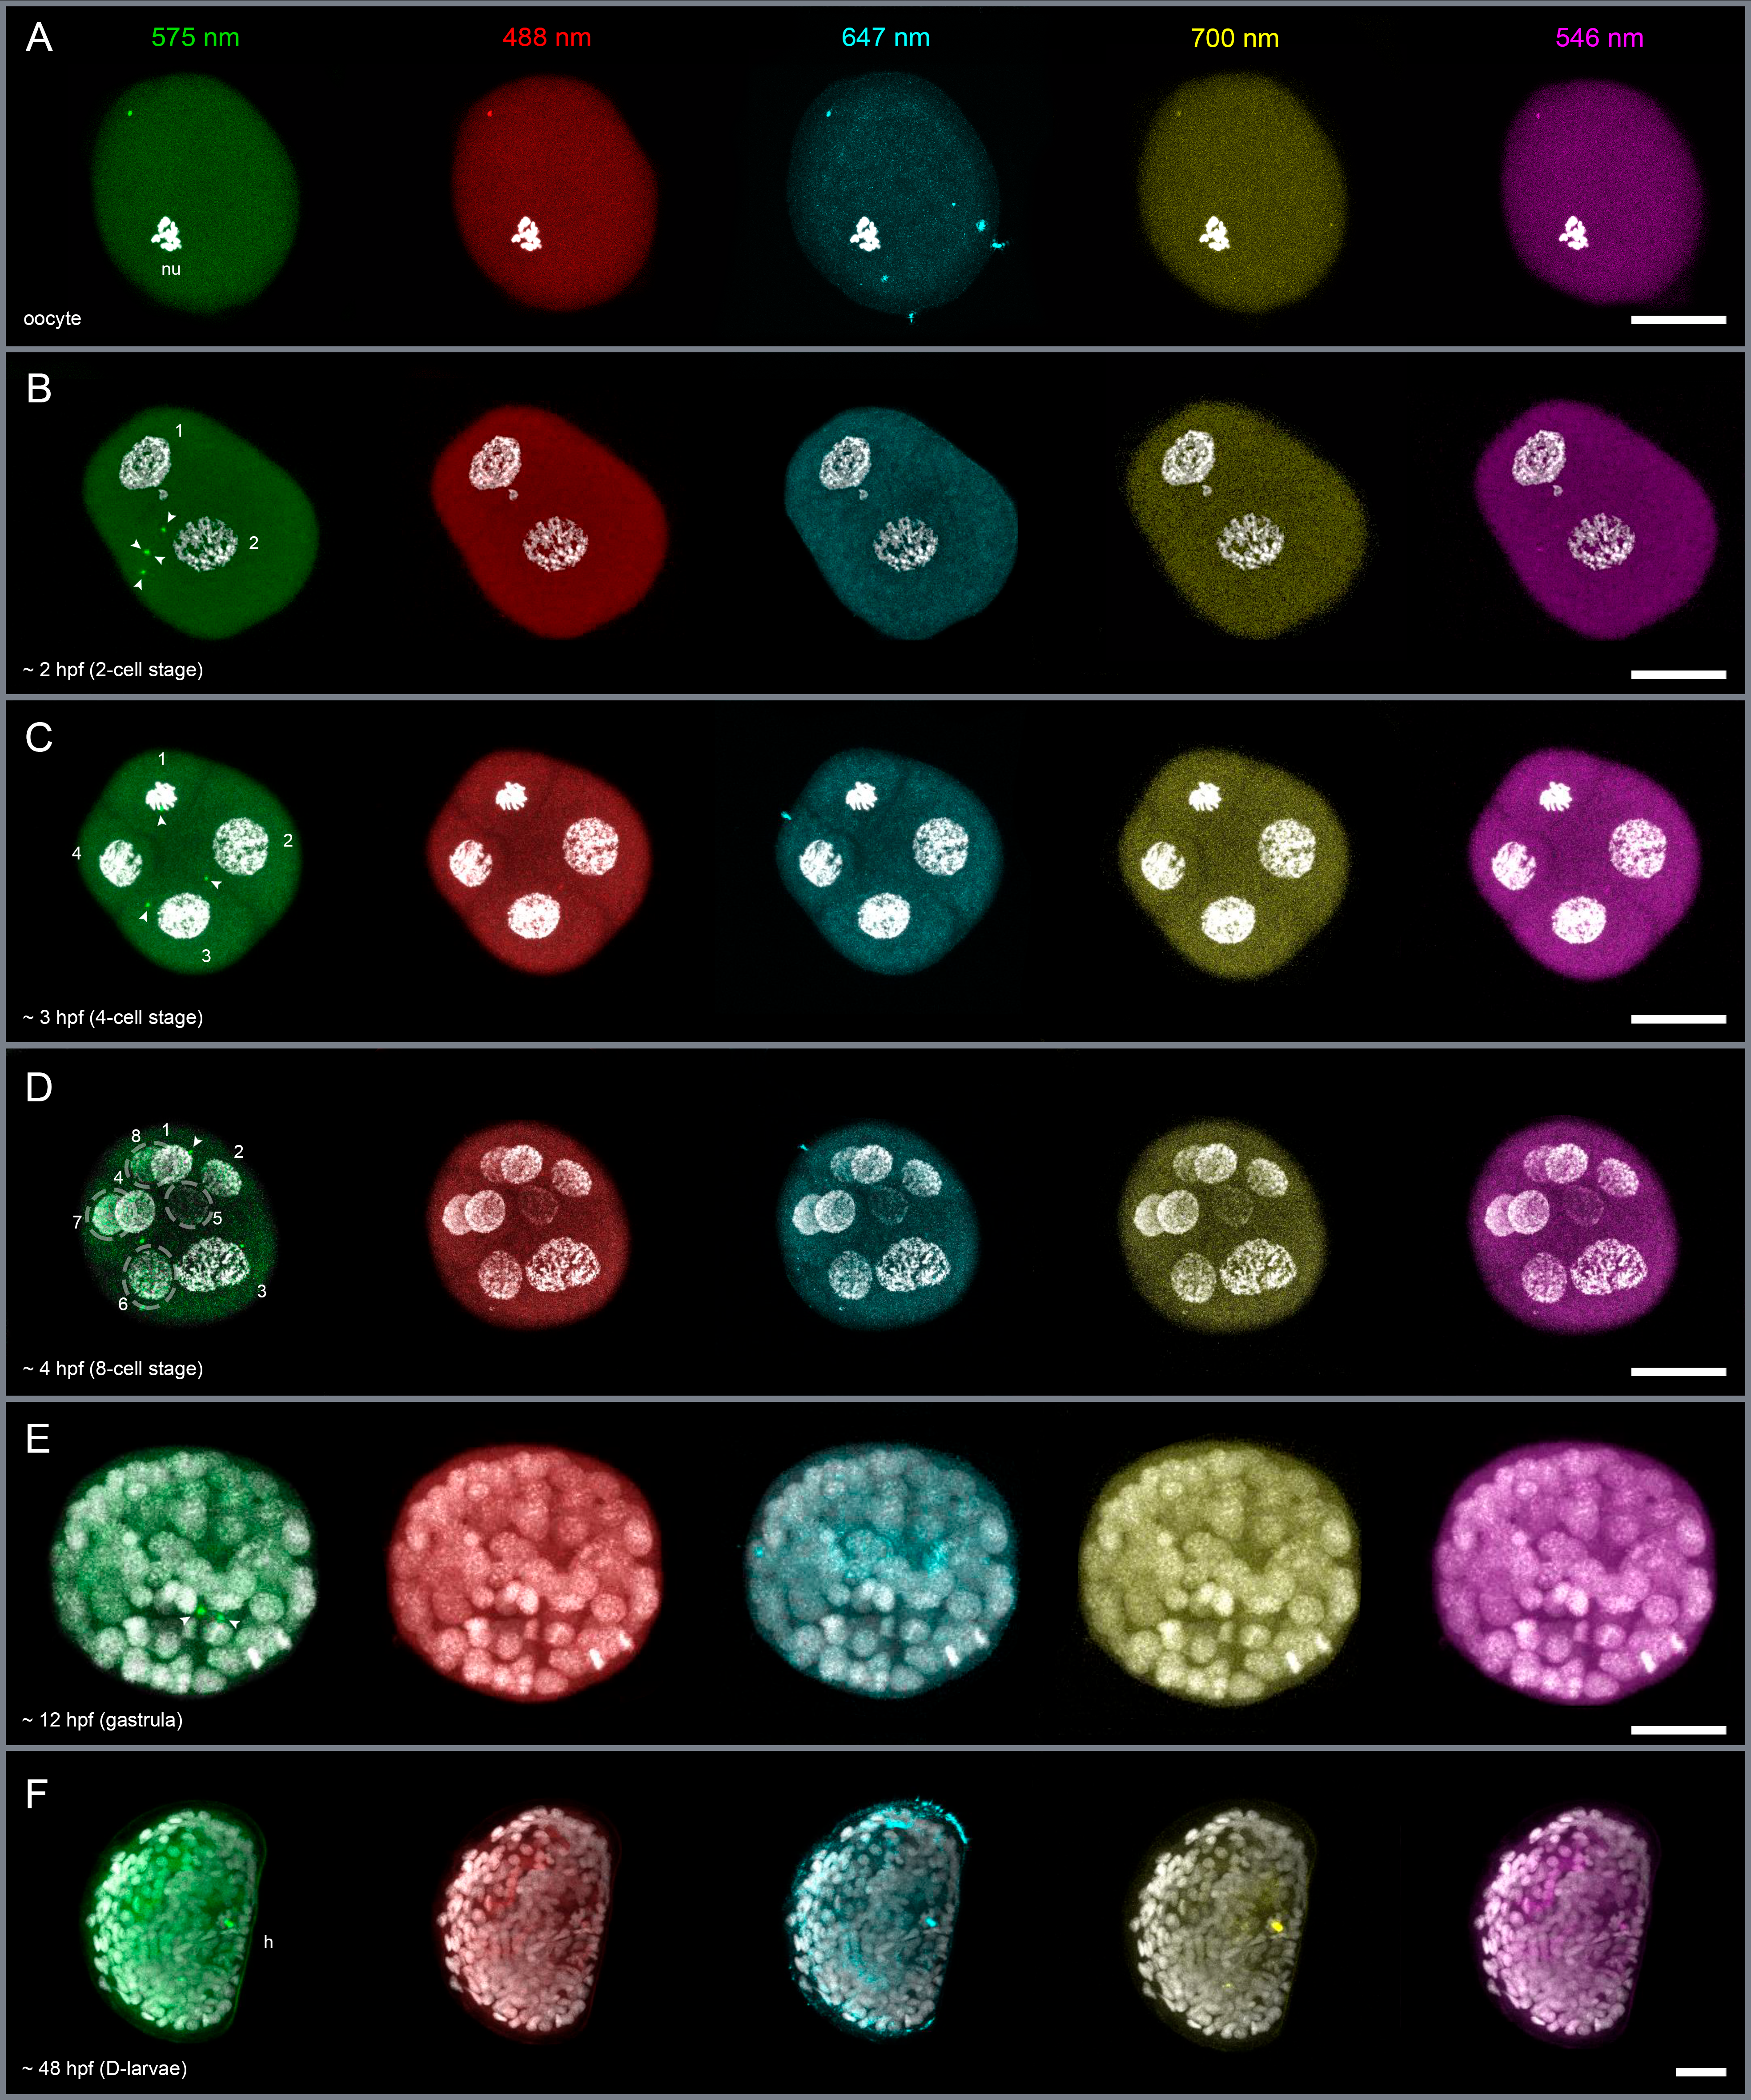
\includegraphics[width=0.9\textwidth]{supp_figures/supp_fig_S16.png}
	\caption[\textbf{MitoTracker staining and negative controls of mRNA \textit{in-situ} \gls{hcr} in in \gls{mgal} (A) oocyte, (B) 2-cell male embryo, (C) 4-cell female embryo, (D) 8-cell female embryo, (E) \qty{12}{\hpf} embryo (gastrula), and (F) \qty{48}{\hpf} larvae (D-veliger)}]
	{
		\textbf{MitoTracker staining and negative controls of mRNA \textit{in-situ} \gls{hcr} in \gls{mgal} (A) oocyte, (B) 2-cell male embryo, (C) 4-cell female embryo, (D) 8-cell female embryo, (E) \qty{12}{\hpf} embryo (gastrula), and (F) \qty{48}{\hpf} larvae (D-veliger)}. Nuclei are shown in white; in the 2-, 4-, and 8-cell stages, nuclei are also marked with numbers; in the 8-cell stage, nuclei of blastomeres in the background are highlighted with dashed circles. Sperm mitochondria, when stained (shown in green), are marked with arrowheads. Acquisition channels are indicated on top, and colours are the same as in \cref{fig:hcr}. h: hinge; nu: oocyte nucleus. Scale bar: \qty{20}{\um}.
	}
	\label{suppFig:hcrBianco}
\end{figure}

\begin{figure}[ht!]
	\floatbox[{\capbeside\thisfloatsetup{capbesideposition={right,top},capbesidewidth=0.4\textwidth}}]{figure}[\FBwidth]
	{\includegraphics[width=0.5\textwidth]{supp_figures/supp_fig_S17.png}}
	{\caption[\textbf{MitoTracker staining and negative controls of Vasa immunolocalization in \gls{mgal} embryos}]
	{
		\textbf{MitoTracker staining and negative controls of Vasa immunolocalization in \gls{mgal} embryos}. Nuclei are shown in white. Sperm mitochondria (in green) are marked with arrowheads. pb: polar body. Scale bar: \qty{20}{\um}.
	}
	\label{suppFig:immunoBianco}}
\end{figure}

\clearpage

\section*{Supplementary tables}
\addcontentsline{toc}{section}{Supplementary tables}

\textit{All the supplementary tables are available in a parsable version at the following GitHub repository: LINK LINK LINK.}

\setcounter{table}{0}
\renewcommand{\tablename}{Supplementary Table}
\renewcommand{\thetable}{\textbf{S\arabic{table}}}

% bivalve dataset
\begin{landscape}
	\setstretch{0.95}
	\tiny
	\begin{longtable}[c]{lllllllllll}
		\caption[\textbf{Genomic and transcriptomic data of bivalves and other molluscs}]
		{
			\textbf{Genomic and transcriptomic data of bivalves and other molluscs}. For each species, the relative ID, taxonomic information, BUSCO statistics, NCBI accession number, and source publication are reported. Biv: Bivalvia; Ca: Caenogastropoda; Cep: Cephalopoda; Co: Coleoidea; Gas: Gastropoda; Gen: Genome; He: Heterobranchia; Im: Imparidentia; Ne: Neomphaliones; Pa: Palaeoheterodonta; Pt: Pteriomorpha; Tra: Transcriptome; Ve: Vetigastropoda
		}
		\label{suppTab:bivalve_dataset}                                                                                                                                                                                                                                                                                                                                                                                                                                                                                                                                                                                                                                                                                              \\
		\toprule
		\textbf{Species}                                                                         & \textbf{ID} & \textbf{Class} & \textbf{Group} & \textbf{Order}    & \textbf{Type} & \textbf{\begin{tabular}[c]{@{}l@{}}Reduced\\ dataset\end{tabular}} & \textbf{\begin{tabular}[c]{@{}l@{}}BUSCO statistics\\ (‘metazoa\_odb10’)\end{tabular}}       & \textbf{NCBI acc. no.}                                                                 & \textbf{Reference}                                                                                                  & \textbf{\begin{tabular}[c]{@{}l@{}}Annotation\\ source\end{tabular}}                                                                                         \\* \midrule \midrule
		\endfirsthead
		%
		\multicolumn{11}{c}%
		{\textbf{Tab. \thetable}\ continued from previous page}                                                                                                                                                                                                                                                                                                                                                                                                                                                                                                                                                                                                                                                                  \\
		\toprule
		\textbf{Species}                                                                         & \textbf{ID} & \textbf{Class} & \textbf{Group} & \textbf{Order}    & \textbf{Type} & \textbf{\begin{tabular}[c]{@{}l@{}}Reduced\\ dataset\end{tabular}} & \textbf{\begin{tabular}[c]{@{}l@{}}BUSCO statistics\\ (‘metazoa\_odb10’)\end{tabular}}       & \textbf{NCBI acc. no.}                                                                 & \textbf{Reference}                                                                                                  & \textbf{\begin{tabular}[c]{@{}l@{}}Annotation\\ source\end{tabular}}                                                                                         \\* \midrule \midrule\endhead
		%
		\textit{\begin{tabular}[c]{@{}l@{}}Magallana (Crassostrea)\\angulata\end{tabular}}       & Cang        & Biv            & Pt             & Ostreida          & Gen           & No                                                                 & \begin{tabular}[c]{@{}l@{}}C:99.1\%{[}S:97.1\%,D:2.0\%{]},\\F:0.3\%,M:0.6\%\end{tabular}   & GCF\_025612915.1                                                                       & \citebold{teng2023parallel}                                                                                    & \href{https://www.ncbi.nlm.nih.gov/datasets/genome/GCF_025612915.1/}{NCBI}                                                                                   \\ [0.4cm]
		\textit{\begin{tabular}[c]{@{}l@{}}Magallana (Crassostrea)\\gigas\end{tabular}}          & Cgig        & Biv            & Pt             & Ostreida          & Gen           & Yes                                                                & \begin{tabular}[c]{@{}l@{}}C:98.2\%{[}S:93.1\%,D:5.1\%{]},\\F:0.4\%,M:1.4\%\end{tabular}   & GCF\_902806645.1                                                                       & \citebold{penaloza2021chromosome}                                                                              & \href{https://www.ncbi.nlm.nih.gov/datasets/genome/GCF_902806645.1/}{NCBI}                                                                                   \\ [0.4cm]
		\textit{\begin{tabular}[c]{@{}l@{}}Magallana (Crassostrea)\\ariakensis\end{tabular}}     & Cari        & Biv            & Pt             & Ostreida          & Gen           & No                                                                 & \begin{tabular}[c]{@{}l@{}}C:94.8\%{[}S:91.2\%,D:3.6\%{]},\\F:0.7\%,M:4.5\%\end{tabular}   & GCA\_020567875.1                                                                       & \citebold{li2021genome}                                                                                        & \href{https://figshare.com/articles/dataset/Genome_of_the_estuarine_oyster_provides_insights_into_climate_impact_and_adaptive_plasticity/16557390}{FigShare} \\ [0.4cm]
		\textit{Crassostrea virginica}                                                           & Cvir        & Biv            & Pt             & Ostreida          & Gen           & Yes                                                                & \begin{tabular}[c]{@{}l@{}}C:98.2\%{[}S:73.1\%,D:25.1\%{]},\\F:0.3\%,M:1.5\%\end{tabular}  & GCF\_002022765.2                                                                       & \citebold{gomez2015developing}                                                                                 & \href{https://www.ncbi.nlm.nih.gov/datasets/genome/GCF_002022765.2/}{NCBI}                                                                                   \\ [0.4cm]
		\textit{Ostrea edulis}                                                                   & Oedu        & Biv            & Pt             & Ostreida          & Gen           & Yes                                                                & \begin{tabular}[c]{@{}l@{}}C:98.7\%{[}S:97.8\%,D:0.9\%{]},\\F:0.5\%,M:0.8\%\end{tabular}   & GCF\_947568905.1                                                                       & Darwin Tree of Life                                                                                        & \href{https://www.ncbi.nlm.nih.gov/datasets/genome/GCF_947568905.1/}{NCBI}                                                                                   \\ [0.4cm]
		\textit{Saccostrea glomerata}                                                            & Sglo        & Biv            & Pt             & Ostreida          & Gen           & No                                                                 & \begin{tabular}[c]{@{}l@{}}C:89.1\%{[}S:85.5\%,D:3.6\%{]},\\F:4.9\%,M:6.0\%\end{tabular}   & GCA\_003671525.1                                                                       & \citebold{powell2018genome}                                                                                    & \href{http://soft.bioinfo-minzhao.org/srog/}{dbSROG}                                                                                                         \\ [0.4cm]
		\textit{Atrina pectinata}                                                                & Apec        & Biv            & Pt             & Ostreida          & Tra           & Yes                                                                & \begin{tabular}[c]{@{}l@{}}C:95.6\%{[}S:93.1\%,D:2.5\%{]},\\F:1.9\%,M:2.5\%\end{tabular}   & DRR348924, -25, -26                                                                    & \citebold{shimizu2022evolution}                                                                                & \NA                                                                                                                                                          \\ [0.4cm]
		\textit{Pinctada margaritifera}                                                          & Pmar        & Biv            & Pt             & Ostreida          & Tra           & Yes                                                                & \begin{tabular}[c]{@{}l@{}}C:94.3\%{[}S:93.9\%,D:0.4\%{]},\\F:1.7\%,M:4.0\%\end{tabular}   & \begin{tabular}[c]{@{}l@{}}SRR1039667\\SRR1041217\end{tabular}                         & \citebold{teaniniuraitemoana2014gonad}                                                                         & \NA                                                                                                                                                          \\ [0.4cm]
		\textit{Mytilus galloprovincialis}                                                       & Mgal        & Biv            & Pt             & Mytilida          & Gen           & Yes                                                                & \begin{tabular}[c]{@{}l@{}}C:80.5\%{[}S:50.4\%,D:30.1\%{]},\\F:8.6\%,M:10.9\%\end{tabular} & GCA\_900618805.1                                                                       & \citebold{gerdol2020massive}                                                                                   & \href{https://www.ncbi.nlm.nih.gov/assembly/GCA_900618805.1/}{NCBI}                                                                                          \\ [0.4cm]
		\textit{Mytilus edulis}                                                                  & Medu        & Biv            & Pt             & Mytilida          & Gen           & No                                                                 & \begin{tabular}[c]{@{}l@{}}C:83.8\%{[}S:70.9\%,D:12.9\%{]},\\F:5.1\%,M:11.1\%\end{tabular} & GCA\_905397895.1                                                                       & \citebold{corrochano2022evidence}                                                                              & \href{https://www.ncbi.nlm.nih.gov/assembly/GCA_905397895.1/}{NCBI}                                                                                          \\ [0.4cm]
		\textit{\begin{tabular}[c]{@{}l@{}}Mytilus unguiculatus\\(coruscus)\end{tabular}}        & Mcor        & Biv            & Pt             & Mytilida          & Gen           & No                                                                 & \begin{tabular}[c]{@{}l@{}}C:80.8\%{[}S:78.8\%,D:2.0\%{]},\\F:4.3\%,M:14.9\%\end{tabular}  & GCA\_011752425.2                                                                       & \citebold{yang2021chromosome}                                                                                  & \href{https://www.ncbi.nlm.nih.gov/assembly/GCA_011752425.2/}{NCBI}                                                                                          \\ [0.4cm]
		\textit{Mytilus californianus}                                                           & Mcal        & Biv            & Pt             & Mytilida          & Gen           & No                                                                 & \begin{tabular}[c]{@{}l@{}}C:96.2\%{[}S:95.0\%,D:1.2\%{]},\\F:0.4\%,M:3.4\%\end{tabular}   & GCF\_021869535.1                                                                       & \citebold{paggeot2022reference}                                                                                & \href{https://www.ncbi.nlm.nih.gov/assembly/GCF_021869535.1/}{NCBI}                                                                                          \\ [0.4cm]
		\textit{Perna viridis}                                                                   & Pvir        & Biv            & Pt             & Mytilida          & Gen           & Yes                                                                & \begin{tabular}[c]{@{}l@{}}C:99.4\%{[}S:99.0\%,D:0.4\%{]},\\F:0.2\%,M:0.4\%\end{tabular}   & GCA\_018327765.1                                                                       & \citebold{inoue2021genomics}                                                                                   & \href{https://drive.google.com/drive/folders/1DF_eM3EjwoXy--0U2YM_9QwElFN4ypu5}{Google Drive}                                                                \\ [0.4cm]
		\textit{Modiolus modiolus}                                                               & Mmod        & Biv            & Pt             & Mytilida          & Tra           & Yes                                                                & \begin{tabular}[c]{@{}l@{}}C:95.7\%{[}S:92.3\%,D:3.4\%{]},\\F:2.1\%,M:2.2\%\end{tabular}   & SRR5043294                                                                             & \citebold{meng2018transcriptome}                                                                               & \NA                                                                                                                                                          \\ [0.4cm]
		\textit{Modiolus philippinarum}                                                          & Mphi        & Biv            & Pt             & Mytilida          & Gen           & No                                                                 & \begin{tabular}[c]{@{}l@{}}C:64.9\%{[}S:63.0\%,D:1.9\%{]},\\F:18.8\%,M:16.3\%\end{tabular} & GCA\_002080025.1                                                                       & \citebold{sun2017adaptation}                                                                                   & \href{https://datadryad.org/stash/dataset/doi:10.5061/dryad.h9942}{Dryad}                                                                                    \\ [0.4cm]
		\textit{Perumytilus purpuratus}                                                          & Ppur        & Biv            & Pt             & Mytilida          & Tra           & Yes                                                                & \begin{tabular}[c]{@{}l@{}}C:84.2\%{[}S:83.3\%,D:0.9\%{]},\\F:11.8\%,M:4.0\%\end{tabular}  & SRR4343820                                                                             & \citebold{briones2018novo}                                                                                     & \NA                                                                                                                                                          \\ [0.4cm]
		\textit{\begin{tabular}[c]{@{}l@{}}Argopecten irradians\\concentricus\end{tabular}}      & Airc        & Biv            & Pt             & Pectinida         & Gen           & Yes                                                                & \begin{tabular}[c]{@{}l@{}}C:94.9\%{[}S:94.0\%,D:0.9\%{]},\\F:3.6\%,M:1.5\%\end{tabular}   & GCA\_004382765.1                                                                       & \citebold{liu2020draft}                                                                                        & \href{https://datadryad.org/stash/dataset/doi:10.5061/dryad.hdr7sqvdr}{Dryad}                                                                                \\ [0.4cm]
		\textit{Argopecten purpuratus}                                                           & Apur        & Biv            & Pt             & Pectinida         & Gen           & No                                                                 & \begin{tabular}[c]{@{}l@{}}C:89.2\%{[}S:88.6\%,D:0.6\%{]},\\F:5.0\%,M:5.8\%\end{tabular}   & \NA                                                                                    & \citebold{liu2020draft}                                                                                        & \href{http://gigadb.org/dataset/100419}{GigaDB}                                                                                                              \\ [0.4cm]
		\textit{Pecten maximus}                                                                  & Pmax        & Biv            & Pt             & Pectinida         & Gen           & Yes                                                                & \begin{tabular}[c]{@{}l@{}}C:98.5\%{[}S:94.5\%,D:4.0\%{]},\\F:0.4\%,M:1.1\%\end{tabular}   & GCF\_902652985.1                                                                       & \citebold{kenny2020gene}                                                                                       & \href{https://www.ncbi.nlm.nih.gov/assembly/GCF_902652985.1/}{NCBI}                                                                                          \\ [0.4cm]
		\textit{\begin{tabular}[c]{@{}l@{}}Mizuhopecten\\(Patinopecten) yessoensis\end{tabular}} & Pyes        & Biv            & Pt             & Pectinida         & Gen           & Yes                                                                & \begin{tabular}[c]{@{}l@{}}C:98.3\%{[}S:96.1\%,D:2.2\%{]},\\F:0.5\%,M:1.2\%\end{tabular}   & GCF\_002113885.1                                                                       & \citebold{wang2017scallop}                                                                                     & \href{https://www.ncbi.nlm.nih.gov/assembly/GCF_002113885.1/}{NCBI}                                                                                          \\ [0.4cm]
		\textit{\begin{tabular}[c]{@{}l@{}}Anadara (Scapharca)\\broughtonii\end{tabular}}        & Sbro        & Biv            & Pt             & Arcida            & Gen           & Yes                                                                & \begin{tabular}[c]{@{}l@{}}C:91.2\%{[}S:85.6\%,D:5.6\%{]},\\F:2.6\%,M:6.2\%\end{tabular}   & \NA                                                                                    & \citebold{bai2019chromosomal}                                                                                  & \href{http://gigadb.org/dataset/100607}{GigaDB}                                                                                                              \\ [0.4cm]
		\textit{Tegillarca granosa}                                                              & Tgra        & Biv            & Pt             & Arcida            & Gen           & Yes                                                                & \begin{tabular}[c]{@{}l@{}}C:70.6\%{[}S:61.3\%,D:9.3\%{]},\\F:11.7\%,M:17.7\%\end{tabular} & GCA\_029721355.1                                                                       & \NA                                                                                                        & \href{https://www.ncbi.nlm.nih.gov/assembly/GCA_029721355.1/}{NCBI}                                                                                          \\ [0.4cm]
		\textit{Ruditapes decussatus}                                                            & Rdec        & Biv            & Im             & Venerida          & Tra           & Yes                                                                & \begin{tabular}[c]{@{}l@{}}C:84.8\%{[}S:84.1\%,D:0.7\%{]},\\F:7.3\%,M:7.9\%\end{tabular}   & \begin{tabular}[c]{@{}l@{}}SRR527740, -41, -43,\\-44, -47, -51, -52, -57\end{tabular}  & \citebold{ghiselli2018comparative}                                                                             & \NA                                                                                                                                                          \\ [0.4cm]
		\textit{Ruditapes philippinarum}                                                         & Rphi        & Biv            & Im             & Venerida          & Gen           & Yes                                                                & \begin{tabular}[c]{@{}l@{}}C:97.8\%{[}S:85.5\%,D:12.3\%{]},\\F:0.7\%,M:1.5\%\end{tabular}  & GCF\_026571515.1                                                                       & \citebold{xu2022multi}                                                                                         & \href{https://www.ncbi.nlm.nih.gov/assembly/GCF_026571515.1/}{NCBI}                                                                                          \\ [0.4cm]
		\textit{Mercenaria mercenaria}                                                           & Mmer        & Biv            & Im             & Venerida          & Gen           & Yes                                                                & \begin{tabular}[c]{@{}l@{}}C:96.0\%{[}S:89.8\%,D:6.2\%{]},\\F:1.0\%,M:3.0\%\end{tabular}   & GCF\_021730395.1                                                                       & \citebold{farhat2022comparative}                                                                               & \href{https://www.ncbi.nlm.nih.gov/assembly/GCF_021730395.1/}{NCBI}                                                                                          \\ [0.4cm]
		\textit{Cyclina sinensis}                                                                & Csin        & Biv            & Im             & Venerida          & Gen           & Yes                                                                & \begin{tabular}[c]{@{}l@{}}C:94.1\%{[}S:83.9\%,D:10.2\%{]},\\F:1.8\%,M:4.1\%\end{tabular}  & GCA\_012932295.1                                                                       & \citebold{wei2020chromosome}                                                                                   & \href{https://datadryad.org/stash/dataset/doi:10.5061/dryad.hdr7sqvdr}{Dryad}                                                                                \\ [0.4cm]
		\textit{\begin{tabular}[c]{@{}l@{}}Calyptogena (Archivesica)\\marissinica\end{tabular}}  & Amar        & Biv            & Im             & Venerida          & Gen           & No                                                                 & \begin{tabular}[c]{@{}l@{}}C:82.1\%{[}S:80.1\%,D:2.0\%{]},\\F:6.0\%,M:11.9\%\end{tabular}  & GCA\_014843695.1                                                                       & \citebold{ip2021host}                                                                                          & \href{https://figshare.com/articles/dataset/Host-Endosymbiont_Genome_Integration_in_a_Deep-Sea_Chemosymbiotic_Clam/12198987}{FigShare}                       \\ [0.4cm]
		\textit{Phreagena okutanii}                                                              & Poku        & Biv            & Im             & Venerida          & Tra           & Yes                                                                & \begin{tabular}[c]{@{}l@{}}C:92.9\%{[}S:85.8\%,D:7.1\%{]},\\F:3.0\%,M:4.1\%\end{tabular}   & \begin{tabular}[c]{@{}l@{}}SRR7156763, -64, -65,\\-66, -67, -68\end{tabular}           & \citebold{lan2019host}                                                                                         & \NA                                                                                                                                                          \\ [0.4cm]
		\textit{Corbicula fluminea}                                                              & Cflu        & Biv            & Im             & Venerida          & Tra           & Yes                                                                & \begin{tabular}[c]{@{}l@{}}C:83.7\%{[}S:79.9\%,D:3.8\%{]},\\F:10.3\%,M:6.0\%\end{tabular}  & \begin{tabular}[c]{@{}l@{}}SRR1559272\\SRR5512046\end{tabular}                         & \begin{tabular}[c]{@{}l@{}}\citebold{gonzalez2015phylogenetic}\\ \citebold{zhu2019transcriptome}\end{tabular} & \NA                                                                                                                                                          \\ [0.4cm]
		\textit{Mactra chinensis}                                                                & Mchi        & Biv            & Im             & Venerida          & Tra           & Yes                                                                & \begin{tabular}[c]{@{}l@{}}C:81.5\%{[}S:80.8\%,D:0.7\%{]},\\F:10.2\%,M:8.3\%\end{tabular}  & SRR1263980                                                                             & \NA                                                                                                                 & \NA                                                                                                                                                          \\ [0.4cm]
		\textit{Mya arenaria}                                                                    & Mare        & Biv            & Im             & Myida             & Gen           & Yes                                                                & \begin{tabular}[c]{@{}l@{}}C:98.5\%{[}S:80.4\%,D:18.1\%{]},\\F:0.4\%,M:1.1\%\end{tabular}  & GCF\_026914265.1                                                                       & \citebold{hart2023centuries}                                                                                   & \href{https://www.ncbi.nlm.nih.gov/assembly/GCF_026914265.1/}{NCBI}                                                                                          \\ [0.4cm]
		\textit{Dreissena polymorpha}                                                            & Dpol        & Biv            & Im             & Myida             & Gen           & Yes                                                                & \begin{tabular}[c]{@{}l@{}}C:97.2\%{[}S:80.1\%,D:17.1\%{]},\\F:0.4\%,M:2.4\%\end{tabular}  & GCF\_020536995.1                                                                       & \citebold{mccartney2022genome}                                                                                 & \href{https://www.ncbi.nlm.nih.gov/assembly/GCF_020536995.1/}{NCBI}                                                                                          \\ [0.4cm]
		\textit{Pisidium coreanum}                                                               & Pcor        & Biv            & Im             & Sphaeriida        & Tra           & Yes                                                                & \begin{tabular}[c]{@{}l@{}}C:94.5\%{[}S:81.6\%,D:12.9\%{]},\\F:3.6\%,M:1.9\%\end{tabular}  & SRR6474597                                                                             & \NA                                                                                                                 & \NA                                                                                                                                                          \\ [0.4cm]
		\textit{Solen grandis}                                                                   & Sgra        & Biv            & Im             & Adapedonta        & Tra           & Yes                                                                & \begin{tabular}[c]{@{}l@{}}C:92.7\%{[}S:90.0\%,D:2.7\%{]},\\F:2.5\%,M:4.8\%\end{tabular}   & SRR5484647, SRR5485368, SRR5499447                                                     & \citebold{nie2018rna}                                                                                          & \NA                                                                                                                                                          \\ [0.4cm]
		\textit{Sinonovacula constricta}                                                         & Scon        & Biv            & Im             & Adapedonta        & Gen           & Yes                                                                & \begin{tabular}[c]{@{}l@{}}C:90.8\%{[}S:79.2\%,D:11.6\%{]},\\F:3.5\%,M:5.7\%\end{tabular}  & GCA\_007844125.1                                                                       & \citebold{ran2019chromosome}                                                                                   & \href{https://datadryad.org/stash/dataset/doi:10.5061/dryad.qv9s4mwc6}{Dryad}                                                                                \\ [0.4cm]
		\textit{Panopea generosa}                                                                & Pgen        & Biv            & Im             & Adapedonta        & Tra           & Yes                                                                & \begin{tabular}[c]{@{}l@{}}C:84.1\%{[}S:81.9\%,D:2.2\%{]},\\F:9.7\%,M:6.2\%\end{tabular}   & SRR12218869, -70                                                                       & \citebold{putnam2022dynamic}                                                                                   & \NA                                                                                                                                                          \\ [0.4cm]
		\textit{Tridacna squamosa}                                                               & Tsqu        & Biv            & Im             & Cardiida          & Tra           & Yes                                                                & \begin{tabular}[c]{@{}l@{}}C:89.7\%{[}S:86.9\%,D:2.8\%{]},\\F:3.5\%,M:6.8\%\end{tabular}   & SRR10824662, -65                                                                       & \citebold{li2020comparative}                                                                                   & \NA                                                                                                                                                          \\ [0.4cm]
		\textit{Loripes orbiculatus}                                                             & Lorb        & Biv            & Im             & Lucinida          & Tra           & Yes                                                                & \begin{tabular}[c]{@{}l@{}}C:76.1\%{[}S:74.9\%,D:1.2\%{]},\\F:14.3\%,M:9.6\%\end{tabular}  & SRR10002336, -38, -39, -47                                                             & \citebold{yuen2019organ}                                                                                       & \NA                                                                                                                                                          \\ [0.4cm]
		\textit{\begin{tabular}[c]{@{}l@{}}Hyriopsis bialata\\(Unio delphinus)\end{tabular}}     & Hbia        & Biv            & Pa             & Unionida          & Gen           & Yes                                                                & \begin{tabular}[c]{@{}l@{}}C:97.5\%{[}S:94.9\%,D:2.6\%{]},\\F:2.0\%,M:0.5\%\end{tabular}   & GCA\_029339505.1                                                                       & \citebold{gomes2023pacbio}                                                                                     & \href{https://figshare.com/s/cc8afa67637d2189e1ae}{FigShare}                                                                                                 \\ [0.4cm]
		\textit{Cristaria plicata}                                                               & Cpli        & Biv            & Pa             & Unionida          & Tra           & Yes                                                                & \begin{tabular}[c]{@{}l@{}}C:93.6\%{[}S:92.8\%,D:0.8\%{]},\\F:2.1\%,M:4.3\%\end{tabular}   & \begin{tabular}[c]{@{}l@{}}SRR2175868\\SRR3095781\end{tabular}                         & \begin{tabular}[c]{@{}l@{}}\citebold{patnaik2016sequencing}\\ \citebold{wang2017transcriptome}\end{tabular} & \NA                                                                                                                                                          \\ [0.4cm]
		\textit{Megalonaias nervosa}                                                             & Mner        & Biv            & Pa             & Unionida          & Gen           & Yes                                                                & \begin{tabular}[c]{@{}l@{}}C:65.0\%{[}S:63.3\%,D:1.7\%{]},\\F:14.0\%,M:21.0\%\end{tabular} & GCA\_016617855.1                                                                       & \citebold{rogers2021gene}                                                                                      & \href{https://datadryad.org/stash/dataset/doi:10.5061/dryad.bzkh1897b}{Dryad}                                                                                \\ [0.4cm]
		\textit{Potamilus streckersoni}                                                          & Pstr        & Biv            & Pa             & Unionida          & Gen           & Yes                                                                & \begin{tabular}[c]{@{}l@{}}C:94.9\%{[}S:93.4\%,D:1.5\%{]},\\F:1.2\%,M:3.9\%\end{tabular}   & GCA\_016746295.1                                                                       & \citebold{smith2021high}                                                                                       & \href{https://www.ncbi.nlm.nih.gov/assembly/GCA_016746295.1}{NCBI}                                                                                           \\ [0.4cm]
		\textit{Margaritifera margaritifera}                                                     & Mmar        & Biv            & Pa             & Unionida          & Gen           & Yes                                                                & \begin{tabular}[c]{@{}l@{}}C:92.6\%{[}S:92.1\%,D:0.5\%{]},\\F:3.0\%,M:4.4\%\end{tabular}   & GCA\_015947965.1                                                                       & \citebold{gomes2021crown}                                                                                      & \href{https://figshare.com/articles/dataset/Margaritifera_margaritifera_whole_genome_assembly_and_annotation/13333841/1}{FigShare}                           \\ [0.4cm]
		\textit{Aplysia californica}                                                             & Acal        & Gas            & He             & Aplysiida         & Gen           & No                                                                 & \begin{tabular}[c]{@{}l@{}}C:97.8\%{[}S:97.0\%,D:0.8\%{]},\\F:0.7\%,M:1.5\%\end{tabular}   & GCF\_000002075.1                                                                       & \citebold{knudsen2006complete}                                                                                 & \href{https://www.ncbi.nlm.nih.gov/assembly/GCF_000002075.1/}{NCBI}                                                                                          \\ [0.4cm]
		\textit{Biomphalaria glabrata}                                                           & Bgla        & Gas            & He             & \NA               & Gen           & No                                                                 & \begin{tabular}[c]{@{}l@{}}C:98.9\%{[}S:98.2\%,D:0.7\%{]},\\F:0.1\%,M:1.0\%\end{tabular}   & GCF\_947242115.1                                                                       & \NA                                                                                                                 & \href{https://www.ncbi.nlm.nih.gov/assembly/GCF_947242115.1/}{NCBI}                                                                                          \\ [0.4cm]
		\textit{Pomacea canaliculata}                                                            & Pcan        & Gas            & Ca             & Architaenioglossa & Gen           & No                                                                 & \begin{tabular}[c]{@{}l@{}}C:98.2\%{[}S:97.0\%,D:1.2\%{]},\\F:0.4\%,M:1.4\%\end{tabular}   & GCF\_003073045.1                                                                       & \citebold{liu2018genome}                                                                                       & \href{https://www.ncbi.nlm.nih.gov/assembly/GCF_003073045.1/}{NCBI}                                                                                          \\ [0.4cm]
		\textit{Gigantopelta aegis}                                                              & Gaeg        & Gas            & Ne             & Neomphalida       & Gen           & No                                                                 & \begin{tabular}[c]{@{}l@{}}C:98.4\%{[}S:94.2\%,D:4.2\%{]},\\F:0.8\%,M:0.8\%\end{tabular}   & GCF\_016097555.1                                                                       & \citebold{lan2021hologenome}                                                                                   & \href{https://www.ncbi.nlm.nih.gov/assembly/GCF_016097555.1/}{NCBI}                                                                                          \\ [0.4cm]
		\textit{Haliotis rufescens}                                                              & Hruf        & Gas            & Ve             & Lepetellida       & Gen           & No                                                                 & \begin{tabular}[c]{@{}l@{}}C:99.0\%{[}S:98.3\%,D:0.7\%{]},\\F:0.0\%,M:1.0\%\end{tabular}   & GCF\_023055435.1                                                                       & \NA                                                                                                                 & \href{https://www.ncbi.nlm.nih.gov/assembly/GCF_023055435.1/}{NCBI}                                                                                          \\ [0.4cm]
		\textit{Octopus bimaculoides}                                                            & Obim        & Cep            & Co             & Octopoda          & Gen           & No                                                                 & \begin{tabular}[c]{@{}l@{}}C:94.9\%{[}S:94.4\%,D:0.5\%{]},\\F:2.3\%,M:2.8\%\end{tabular}   & GCF\_001194135.2                                                                       & \citebold{albertin2015octopus}                                                                                 & \href{https://www.ncbi.nlm.nih.gov/assembly/GCF_001194135.2/}{NCBI}                                                                                          \\ [0.4cm]
		\textit{Octopus sinensis}                                                                & Osin        & Cep            & Co             & Octopoda          & Gen           & No                                                                 & \begin{tabular}[c]{@{}l@{}}C:98.1\%{[}S:96.9\%,D:1.2\%{]},\\F:0.9\%,M:1.0\%\end{tabular}   & GCF\_006345805.1                                                                       & \citebold{li2020chromosome}                                                                                    & \href{https://www.ncbi.nlm.nih.gov/assembly/GCF_006345805.1/}{NCBI}                                                                                          \\* \bottomrule \bottomrule
	\end{longtable}
\end{landscape}

% PANTHER and CDD accessions
\begin{landscape}
	\tiny
	\setstretch{0.95}
	\begin{longtable}[c]{@{}cllll@{}}
		\caption[\textbf{\gls{dsfg} family and domain identifiers (IDs) in PANTHER and CDD, respectively}]
		{
			\textbf{\gls{dsfg} family and domain identifiers (IDs) in PANTHER and CDD, respectively}. After having retrieved putative \glspl{dsfg} on the basis of \gls{hmm} profiles, IDs have been used to retain only reliable hits.
		}
		\label{suppTab:panther_cdd}                                                                                                                                                                                               \\
		\toprule
		\textbf{Gene family}            & \textbf{PANTHER/CDD} & \textbf{ID}     & \textbf{Description}                                                                                                                         & \\* \midrule \midrule
		\endfirsthead
		%
		\multicolumn{5}{c}%
		{\textbf{Tab. \thetable}\ continued from previous page}                                                                                                                                                               \\
		\toprule
		\textbf{Gene family}            & \textbf{PANTHER/CDD} & \textbf{ID}     & \textbf{Description}                                                                                                                         & \\* \midrule \midrule
		\endhead
		%
		\multirow{12}{*}{\textbf{Dmrt}} & CDD                  & gnl|CDD|214606  & Doublesex DNA-binding motif                                                                                                                  & \\
		                                & CDD                  & gnl|CDD|425850  & DM DNA binding domain                                                                                                                        & \\
		                                & PANTHER              & PTHR12322       & DOUBLESEX AND MAB-3 RELATED TRANSCRIPTION FACTOR  DMRT                                                                                       & \\
		                                & PANTHER              & PTHR12322:SF115 & PROTEIN CBR-MAB-23                                                                                                                           & \\
		                                & PANTHER              & PTHR12322:SF116 & DOUBLESEX- AND MAB-3-RELATED TRANSCRIPTION FACTOR 1                                                                                          & \\
		                                & PANTHER              & PTHR12322:SF118 & DOUBLESEX- AND MAB-3-RELATED TRANSCRIPTION FACTOR DMD-4                                                                                      & \\
		                                & PANTHER              & PTHR12322:SF123 & DOUBLESEX-MAB RELATED 99B                                                                                                                    & \\
		                                & PANTHER              & PTHR12322:SF53  & DOUBLESEX- AND MAB-3-RELATED TRANSCRIPTION FACTOR 2                                                                                          & \\
		                                & PANTHER              & PTHR12322:SF71  & DOUBLESEX- AND MAB-3-RELATED TRANSCRIPTION FACTOR A1                                                                                         & \\
		                                & PANTHER              & PTHR16897:SF2   & STRESS RESPONSE PROTEIN NST1                                                                                                                 & \\
		                                & PANTHER              & PTHR46888:SF11  & RIBONUCLEASE H                                                                                                                               & \\* \midrule
		\multirow{38}{*}{\textbf{Sox}}  & CDD                  & gnl|CDD|432488  & SOX transcription factor                                                                                                                     & \\
		                                & CDD                  & gnl|CDD|432558  & Sox developmental protein N terminal                                                                                                         & \\
		                                & CDD                  & gnl|CDD|438790  & high mobility group (HMG)-box found in group B SRY-related high-mobility group (HMG) box (Sox) transcription factors                         & \\
		                                & CDD                  & gnl|CDD|438820  & high mobility group (HMG)-box found in sex-determining region Y (SRY)-box (SOX) family transcription factors                                 & \\
		                                & CDD                  & gnl|CDD|438837  & high mobility group (HMG)-box found in group A, group B and group G of SRY-related high-mobility group (HMG) box (Sox) transcription factors & \\
		                                & CDD                  & gnl|CDD|438838  & high mobility group (HMG)-box found in group C SRY-related high-mobility group (HMG) box (Sox) transcription factors                         & \\
		                                & CDD                  & gnl|CDD|438839  & high mobility group (HMG)-box found in group D SRY-related high-mobility group (HMG) box (Sox) transcription factors                         & \\
		                                & CDD                  & gnl|CDD|438840  & high mobility group (HMG)-box found in group E SRY-related high-mobility group (HMG) box (Sox) transcription factors                         & \\
		                                & CDD                  & gnl|CDD|438841  & high mobility group (HMG)-box found in group F SRY-related high-mobility group (HMG) box (Sox) transcription factors                         & \\
		                                & CDD                  & gnl|CDD|438842  & high mobility group (HMG)-box found in sex determining region Y (SRY)-box 30 (SOX30) and similar proteins                                    & \\
		                                & CDD                  & gnl|CDD|438843  & high mobility group (HMG)-box found in sex-determining region Y protein (SRY) and similar proteins                                           & \\
		                                & CDD                  & gnl|CDD|438844  & high mobility group (HMG)-box found in sex determining region Y (SRY)-box 15 (SOX15) and similar proteins                                    & \\
		                                & CDD                  & gnl|CDD|438845  & high mobility group (HMG)-box found in sex determining region Y (SRY)-box 4 (SOX4) and similar proteins                                      & \\
		                                & CDD                  & gnl|CDD|438846  & high mobility group (HMG)-box found in sex determining region Y (SRY)-box 11 (SOX11) and similar proteins                                    & \\
		                                & CDD                  & gnl|CDD|438847  & high mobility group (HMG)-box found in sex determining region Y (SRY)-box 12 (SOX12) and similar proteins                                    & \\
		                                & CDD                  & gnl|CDD|438849  & high mobility group (HMG)-box found in sex determining region Y (SRY)-box 7 (SOX7) and similar proteins                                      & \\
		                                & CDD                  & gnl|CDD|438850  & high mobility group (HMG)-box found in sex determining region Y (SRY)-box 17 (SOX17) and similar proteins                                    & \\
		                                & CDD                  & gnl|CDD|438851  & high mobility group (HMG)-box found in sex determining region Y (SRY)-box 18 (SOX18) and similar proteins                                    & \\
		                                & PANTHER              & PTHR10270:SF107 & TRANSCRIPTION FACTOR SOX-14                                                                                                                  & \\
		                                & PANTHER              & PTHR10270:SF161 & SOX DOMAIN-CONTAINING PROTEIN DICHAETE-RELATED                                                                                               & \\
		                                & PANTHER              & PTHR10270:SF199 & SEX-DETERMINING REGION Y PROTEIN                                                                                                             & \\
		                                & PANTHER              & PTHR10270:SF231 & TRANSCRIPTION FACTOR SOX-2                                                                                                                   & \\
		                                & PANTHER              & PTHR10270:SF27  & TRANSCRIPTION FACTOR SOX-4                                                                                                                   & \\
		                                & PANTHER              & PTHR10270:SF313 & TRANSCRIPTION FACTOR SOX-21                                                                                                                  & \\
		                                & PANTHER              & PTHR10270:SF315 & TRANSCRIPTION FACTOR SOX-1A-RELATED                                                                                                          & \\
		                                & PANTHER              & PTHR10270:SF317 & TRANSCRIPTION FACTOR SOX-15-RELATED                                                                                                          & \\
		                                & PANTHER              & PTHR10270:SF322 & TRANSCRIPTION FACTOR SOX-3                                                                                                                   & \\
		                                & PANTHER              & PTHR10270:SF324 & TRANSCRIPTION FACTOR SOX-3                                                                                                                   & \\
		                                & PANTHER              & PTHR10270:SF326 & TRANSCRIPTION FACTOR SOX                                                                                                                     & \\
		                                & PANTHER              & PTHR10270       & SOX TRANSCRIPTION FACTOR                                                                                                                     & \\
		                                & PANTHER              & PTHR45789       & FI18025P1                                                                                                                                    & \\
		                                & PANTHER              & PTHR45789:SF2   & FI18025P1                                                                                                                                    & \\
		                                & PANTHER              & PTHR45803:SF1   & TRANSCRIPTION FACTOR SOX-9                                                                                                                   & \\
		                                & PANTHER              & PTHR45803:SF2   & TRANSCRIPTION FACTOR SOX-8                                                                                                                   & \\
		                                & PANTHER              & PTHR45803:SF5   & SOX100B                                                                                                                                      & \\
		                                & PANTHER              & PTHR45803       & SOX100B                                                                                                                                      & \\
		                                & PANTHER              & PTHR47279:SF1   & TRANSCRIPTION FACTOR SOX-30                                                                                                                  & \\
		                                & PANTHER              & PTHR47279       & TRANSCRIPTION FACTOR SOX-30                                                                                                                  & \\* \midrule
		\multirow{13}{*}{\textbf{Fox}}  & CDD                  & gnl|CDD|410788  & Forkhead (FH) domain found in Forkhead box (FOX) family of transcription factors and similar proteins                                        & \\
		                                & CDD                  & gnl|CDD|410789  & Forkhead (FH) domain found in the Forkhead box protein A (FOXA) subfamily                                                                    & \\
		                                & CDD                  & gnl|CDD|410790  & Forkhead (FH) domain found in the Forkhead box protein B (FOXB) subfamily                                                                    & \\
		                                & CDD                  & gnl|CDD|410791  & Forkhead (FH) domain found in the Forkhead box protein C (FOXC) subfamily                                                                    & \\
		                                & CDD                  & gnl|CDD|410792  & Forkhead (FH) domain found in the Forkhead box protein D (FOXD) subfamily                                                                    & \\
		                                & CDD                  & gnl|CDD|410793  & Forkhead (FH) domain found in the Forkhead box protein E (FOXE) subfamily                                                                    & \\
		                                & CDD                  & gnl|CDD|410794  & Forkhead (FH) domain found in the Forkhead box protein F (FOXF) subfamily                                                                    & \\
		                                & CDD                  & gnl|CDD|410795  & Forkhead (FH) domain found in the Forkhead box protein G (FOXG) subfamily                                                                    & \\
		                                & CDD                  & gnl|CDD|410796  & Forkhead (FH) domain found in the Forkhead box protein H (FOXH) subfamily                                                                    & \\
		                                & CDD                  & gnl|CDD|410797  & Forkhead (FH) domain found in Forkhead box protein J1 (FOXJ1) and similar proteins                                                           & \\
		                                & CDD                  & gnl|CDD|410798  & Forkhead (FH) domain found in Forkhead box proteins, FOXJ2, FOXJ3 and similar proteins                                                       & \\
		                                & CDD                  & gnl|CDD|410799  & Forkhead (FH) domain found in the Forkhead box protein I (FOXI) subfamily                                                                    & \\
		                                & CDD                  & gnl|CDD|410800  & Forkhead (FH) domain found in the Forkhead box protein K (FOXK) subfamily                                                                    & \\
		\multirow{69}{*}{\textbf{Fox}} 	& CDD                  & gnl|CDD|410801  & Forkhead (FH) domain found in Forkhead box protein L1 (FOXL1) and similar proteins                                                           & \\
										& CDD                  & gnl|CDD|410802  & Forkhead (FH) domain found in Forkhead box protein L2 (FOXL2) and similar proteins                                                           & \\
		                                & CDD                  & gnl|CDD|410803  & Forkhead (FH) domain found in the Forkhead box protein M (FOXM) subfamily                                                                    & \\
		                                & CDD                  & gnl|CDD|410804  & Forkhead (FH) domain found in Forkhead box protein N1 (FOXN1) and similar proteins                                                           & \\
		                                & CDD                  & gnl|CDD|410805  & Forkhead (FH) domain found in Forkhead box protein N2 (FOXN2) and similar proteins                                                           & \\
		                                & CDD                  & gnl|CDD|410806  & Forkhead (FH) domain found in the Forkhead box protein O (FOXO) subfamily                                                                    & \\
		                                & CDD                  & gnl|CDD|410807  & Forkhead (FH) domain found in the Forkhead box protein P (FOXP) subfamily                                                                    & \\
		                                & CDD                  & gnl|CDD|410808  & Forkhead (FH) domain found in Forkhead box protein Q1 (FOXQ1) and similar proteins                                                           & \\
		                                & CDD                  & gnl|CDD|410809  & Forkhead (FH) domain found in Forkhead box protein Q2 (FOXQ2) and similar proteins                                                           & \\
		                                & CDD                  & gnl|CDD|410810  & Forkhead (FH) domain found in the Forkhead box protein R (FOXR) subfamily                                                                    & \\
		                                & CDD                  & gnl|CDD|410811  & Forkhead (FH) domain found in Forkhead box protein S1 (FOXS1)                                                                                & \\
		                                & CDD                  & gnl|CDD|410812  & Forkhead (FH) domain found in Forkhead box protein A1 (FOXA1) and similar proteins                                                           & \\
		                                & CDD                  & gnl|CDD|410813  & Forkhead (FH) domain found in Forkhead box protein A2 (FOXA2) and similar proteins                                                           & \\
		                                & CDD                  & gnl|CDD|410814  & Forkhead (FH) domain found in Forkhead box protein A3 (FOXA3) and similar proteins                                                           & \\
		                                & CDD                  & gnl|CDD|410816  & Forkhead (FH) domain found in Forkhead box protein B1 (FOXB1) and similar proteins                                                           & \\
		                                & CDD                  & gnl|CDD|410817  & Forkhead (FH) domain found in Forkhead box protein B2 (FOXB2) and similar proteins                                                           & \\
		                                & CDD                  & gnl|CDD|410818  & Forkhead (FH) domain found in Forkhead box protein C1 (FOXC1) and similar proteins                                                           & \\
		                                & CDD                  & gnl|CDD|410819  & Forkhead (FH) domain found in Forkhead box protein C2 (FOXC2) and similar proteins                                                           & \\
		                                & CDD                  & gnl|CDD|410820  & Forkhead (FH) domain found in Forkhead box proteins FOXD1, FOXD2 and similar proteins                                                        & \\
		                                & CDD                  & gnl|CDD|410821  & Forkhead (FH) domain found in Forkhead box protein D3 (FOXD3) and similar proteins                                                           & \\
		                                & CDD                  & gnl|CDD|410822  & Forkhead (FH) domain found in Forkhead box protein D4 (FOXD4) and similar proteins                                                           & \\
		                                & CDD                  & gnl|CDD|410823  & Forkhead (FH) domain found in Forkhead box protein F1 (FOXF1) and similar proteins                                                           & \\
		                                & CDD                  & gnl|CDD|410824  & Forkhead (FH) domain found in Forkhead box protein F2 (FOXF2) and similar proteins                                                           & \\
		                                & CDD                  & gnl|CDD|410825  & Forkhead (FH) domain found in Forkhead box protein J2 (FOXJ2) and similar proteins                                                           & \\
		                                & CDD                  & gnl|CDD|410826  & Forkhead (FH) domain found in Forkhead box protein J3 (FOXJ3) and similar proteins                                                           & \\
		                                & CDD                  & gnl|CDD|410827  & Forkhead (FH) domain found in Forkhead box protein I1 (FOXI1) and similar proteins                                                           & \\
		                                & CDD                  & gnl|CDD|410828  & Forkhead (FH) domain found in Forkhead box protein K1 (FOXK1) and similar proteins                                                           & \\
		                                & CDD                  & gnl|CDD|410829  & Forkhead (FH) domain found in Forkhead box protein K2 (FOXK2) and similar proteins                                                           & \\
		                                & CDD                  & gnl|CDD|410830  & Forkhead (FH) domain found in Forkhead box protein N1 (FOXN1)                                                                                & \\
		                                & CDD                  & gnl|CDD|410831  & Forkhead (FH) domain found in Forkhead box protein N4 (FOXN4)                                                                                & \\
		                                & CDD                  & gnl|CDD|410832  & Forkhead (FH) domain found in Forkhead box protein N2 (FOXN2)                                                                                & \\
		                                & CDD                  & gnl|CDD|410833  & Forkhead (FH) domain found in Forkhead box protein N3 (FOXN3)                                                                                & \\
		                                & CDD                  & gnl|CDD|410834  & Forkhead (FH) domain found in Forkhead box protein O1 (FOXO1)                                                                                & \\
		                                & CDD                  & gnl|CDD|410835  & Forkhead (FH) domain found in Forkhead box protein O3 (FOXO3)                                                                                & \\
		                                & CDD                  & gnl|CDD|410836  & Forkhead (FH) domain found in Forkhead box protein O4 (FOXO4) and similar proteins                                                           & \\
		                                & CDD                  & gnl|CDD|410837  & Forkhead (FH) domain found in Forkhead box protein O6 (FOXO6) and similar proteins                                                           & \\
		                                & CDD                  & gnl|CDD|410838  & Forkhead (FH) domain found in Forkhead box protein P1 (FOXP1)                                                                                & \\
		                                & CDD                  & gnl|CDD|410839  & Forkhead (FH) domain found in Forkhead box protein P2 (FOXP2)                                                                                & \\
		                                & CDD                  & gnl|CDD|410840  & Forkhead (FH) domain found in Forkhead box protein P3 (FOXP3) and similar proteins                                                           & \\
		                                & CDD                  & gnl|CDD|410841  & Forkhead (FH) domain found in Forkhead box protein P4 (FOXP4) and similar proteins                                                           & \\
		                                & PANTHER              & PTHR11829       & FORKHEAD BOX PROTEIN                                                                                                                         & \\
		                                & PANTHER              & PTHR11829:SF142 & FOXQ2 PROTEIN                                                                                                                                & \\
		                                & PANTHER              & PTHR11829:SF156 & FORKHEAD BOX PROTEIN E3                                                                                                                      & \\
		                                & PANTHER              & PTHR11829:SF206 & FORKHEAD BOX PROTEIN Q1                                                                                                                      & \\
		                                & PANTHER              & PTHR11829:SF209 & FORKHEAD BOX PROTEIN B1                                                                                                                      & \\
		                                & PANTHER              & PTHR11829:SF335 & FORKHEAD BOX PROTEIN D2                                                                                                                      & \\
		                                & PANTHER              & PTHR11829:SF340 & FORKHEAD BOX PROTEIN H1                                                                                                                      & \\
		                                & PANTHER              & PTHR11829:SF342 & FORKHEAD BOX PROTEIN L2                                                                                                                      & \\
		                                & PANTHER              & PTHR11829:SF348 & FORKHEAD BOX PROTEIN D1                                                                                                                      & \\
		                                & PANTHER              & PTHR11829:SF361 & FORKHEAD BOX PROTEIN D3                                                                                                                      & \\
		                                & PANTHER              & PTHR11829:SF398 & FORKHEAD BOX PROTEIN PES-1                                                                                                                   & \\
		                                & PANTHER              & PTHR11829:SF399 & FORKHEAD TRANSCRIPTION FACTOR FKH-9                                                                                                          & \\
		                                & PANTHER              & PTHR11829:SF401 & FORKHEAD BOX C1-A-RELATED                                                                                                                    & \\
		                                & PANTHER              & PTHR13962       & FORKHEAD BOX PROTEIN N3-LIKE PROTEIN-RELATED                                                                                                 & \\
		                                & PANTHER              & PTHR13962:SF17  & FORKHEAD BOX PROTEIN N4                                                                                                                      & \\
		                                & PANTHER              & PTHR13962:SF19  & FORKHEAD BOX PROTEIN N2                                                                                                                      & \\
		                                & PANTHER              & PTHR13962:SF20  & FORKHEAD BOX PROTEIN N3                                                                                                                      & \\
		                                & PANTHER              & PTHR13962:SF22  & FORKHEAD BOX PROTEIN N3-LIKE PROTEIN                                                                                                         & \\
		                                & PANTHER              & PTHR13962:SF26  & FORKHEAD BOX PROTEIN N2                                                                                                                      & \\
		                                & PANTHER              & PTHR45767       & FORKHEAD BOX PROTEIN O                                                                                                                       & \\
		                                & PANTHER              & PTHR45767:SF2   & FORKHEAD BOX PROTEIN O                                                                                                                       & \\
		                                & PANTHER              & PTHR45796       & FORKHEAD BOX P, ISOFORM C                                                                                                                    & \\
		                                & PANTHER              & PTHR45796:SF3   & FORKHEAD BOX PROTEIN P1                                                                                                                      & \\
		                                & PANTHER              & PTHR45796:SF4   & FORKHEAD BOX P, ISOFORM C                                                                                                                    & \\
		                                & PANTHER              & PTHR45881:SF3   & FORKHEAD BOX PROTEIN K2                                                                                                                      & \\
		                                & PANTHER              & PTHR45881:SF4   & FORKHEAD BOX PROTEIN K1                                                                                                                      & \\
		                                & PANTHER              & PTHR46078       & FORKHEAD BOX PROTEIN J2 FAMILY MEMBER                                                                                                        & \\
		                                & PANTHER              & PTHR46262       & FORKHEAD BOX PROTEIN BINIOU                                                                                                                  & \\
		                                & PANTHER              & PTHR46262:SF2   & FORKHEAD BOX PROTEIN BINIOU                                                                                                                  & \\
		\multirow{9}{*}{\textbf{Fox}}	& PANTHER              & PTHR46617       & FORKHEAD BOX PROTEIN G1                                                                                                                      & \\
										& PANTHER              & PTHR46617:SF3   & FORKHEAD BOX PROTEIN G1                                                                                                                      & \\
		                                & PANTHER              & PTHR46721       & FORKHEAD BOX PROTEIN N1                                                                                                                      & \\
		                                & PANTHER              & PTHR46721:SF2   & FORKHEAD BOX N1                                                                                                                              & \\
		                                & PANTHER              & PTHR46805       & FORKHEAD BOX PROTEIN J1                                                                                                                      & \\
		                                & PANTHER              & PTHR46878       & FORKHEAD BOX PROTEIN M1                                                                                                                      & \\
		                                & PANTHER              & PTHR46878:SF1   & FORKHEAD BOX PROTEIN M1                                                                                                                      & \\
		                                & PANTHER              & PTHR47316       & FORKHEAD BOX PROTEIN H1                                                                                                                      & \\
		                                & PANTHER              & PTHR47316:SF1   & FORKHEAD BOX PROTEIN H1                                                                                                                      & \\* \bottomrule \bottomrule
	\end{longtable}
\end{landscape}

% list of referece DSFGs
{
\tiny
\setstretch{0.95}
\begin{longtable}[c]{llll}
	\caption[\textbf{List of \glspl{dsfg} from reference species used to assess the identity of \glspl{dsfg} in molluscs}]
	{
		\textbf{List of \glspl{dsfg} from reference species used to assess the identity of \glspl{dsfg} in molluscs}. NCBI accession numbers are reported in parenthesis. Each row represents an orthology group.
	}
	\label{suppTab:reference_dsfgs}                                                                                                                                                                                                                                                               \\
	\toprule
	\textit{\textbf{Homo sapiens}}                          & \textit{\textbf{Drosophila melanogaster}}                                                              & \textit{\textbf{Caenorhabditis elegans}}                                                           & \textbf{Group}        \\*  \midrule
	\endfirsthead
	%
	\multicolumn{4}{c}%
	{\textbf{Tab. \thetable}\ continued from previous page}                                                                                                                                                                                                                                   \\
	\toprule
	\textit{\textbf{Homo sapiens}}                          & \textit{\textbf{Drosophila melanogaster}}                                                              & \textit{\textbf{Caenorhabditis elegans}}                                                           & \textbf{Group}        \\* \midrule
	\multicolumn{4}{c}{\textbf{Fox gene family}}                                                                                                                                                                                                                                                  \\* \midrule \midrule
	\endhead
	%
	\multicolumn{4}{c}{\textbf{Dmrt gene family}}                                                                                                                                                                                                                                                 \\* \midrule \midrule
	\textit{DMRT1 (NP\_068770.2)}                           & -                                                                                                      & -                                                                                                  & 1                     \\ [0.1cm]
	\textit{DMRT2 (NP\_006548.1)}                           & \textit{dmrt11E (NP\_511146.2)}                                                                        & -                                                                                                  & 2                     \\ [0.1cm]
	\textit{DMRT3 (NP\_067063.1)}                           & \textit{dmrt93B (NP\_524428.1)}                                                                        & \textit{dmd-4 (NP\_510466.1)}                                                                      & 3                     \\ [0.2cm]
	\textit{DMRT4/A1 (NP\_071443.2)}                        & \multirow{2}{*}{\textit{dmrt99b (NP\_524549.1)}}                                                       & \multirow{2}{*}{\textit{dmd-5 (NP\_495138.2)}}                                                     & \multirow{2}{*}{A1/2} \\
	\textit{DMRT5/A2 (NP\_115486.1)}                        &                                                                                                        &                                                                                                    &                       \\ [0.2cm]
	\textit{DMRT6/B1 (NP\_149056.1)}                        & -                                                                                                      & -                                                                                                  & -                     \\ [0.1cm]
	\textit{DMRT7/C2 (NP\_001035373.1)}                     & -                                                                                                      & -                                                                                                  & -                     \\ [0.1cm]
	\textit{DMRT8/C1 (NP\_149042.2)}                        & -                                                                                                      & -                                                                                                  & -                     \\ [0.1cm]
	-                                                       & \textit{dsx (NP\_731197.1)}                                                                            & -                                                                                                  & -                     \\ [0.1cm]
	-                                                       & -                                                                                                      & \textit{mab3 (NP\_001256882.1)}                                                                    & -                     \\ [0.1cm]
	-                                                       & -                                                                                                      & \textit{dmd-3 (NP\_001256883.1)}                                                                   & -                     \\ [0.1cm]
	-                                                       & -                                                                                                      & \textit{dmd-6 (NP\_001370045.1)}                                                                   & -                     \\ [0.1cm]
	-                                                       & -                                                                                                      & \textit{dmd-7 (NP\_741551.1)}                                                                      & -                     \\ [0.1cm]
	-                                                       & -                                                                                                      & \textit{dmd-8 (NP\_503176.2)}                                                                      & -                     \\ [0.1cm]
	-                                                       & -                                                                                                      & \textit{dmd-9 (NP\_500305.1)}                                                                      & -                     \\ [0.1cm]
	-                                                       & -                                                                                                      & \textit{dmd-11 (NP\_001379162.1)}                                                                  & -                     \\ [0.1cm]
	-                                                       & -                                                                                                      & \textit{mab-23 (NP\_001041089.1)}                                                                  & -                     \\* \midrule
	\multicolumn{4}{c}{\textbf{Sox gene family}}                                                                                                                                                                                                                                                  \\* \midrule \midrule
	\textit{SRY (NP\_003131.1)}                             & -                                                                                                      & -                                                                                                  & A                     \\ [0.2cm]
	\textit{SOX3 (NP\_005625.2)}                            & \multirow{3}{*}{\begin{tabular}[c]{@{}l@{}}dichaete (NP\_524066.1)\\ soxN (NP\_524735.1)\end{tabular}} & \multirow{3}{*}{\begin{tabular}[c]{@{}l@{}}sox3 (NP\_510439.1)\\ sox2 (NP\_741836.1)\end{tabular}} & \multirow{3}{*}{B1}   \\
	\textit{SOX2 (NP\_003097.1)}                            &                                                                                                        &                                                                                                    &                       \\
	\textit{SOX1 (NP\_005977.2)}                            &                                                                                                        &                                                                                                    &                       \\ [0.2cm]
	\textit{SOX14 (NP\_004180.1)}                           & \multirow{2}{*}{\begin{tabular}[c]{@{}l@{}}sox21a (NP\_648694.1)\\ sox21b (NP\_648695.1)\end{tabular}} & \multirow{2}{*}{-}                                                                                 & \multirow{2}{*}{B2}   \\
	\textit{SOX21 (NP\_009015.1)}                           &                                                                                                        &                                                                                                    &                       \\ [0.2cm]
	\textit{SOX11 (NP\_003099.1)}                           & \multirow{3}{*}{\textit{sox14 (NP\_476894.1)}}                                                         & \multirow{3}{*}{\textit{sem-2 (NP\_740846.1)}}                                                     & \multirow{3}{*}{C}    \\
	\textit{SOX12 (NP\_008874.2)}                           &                                                                                                        &                                                                                                    &                       \\
	\textit{SOX4 (NP\_003098.1)}                            &                                                                                                        &                                                                                                    &                       \\ [0.2cm]
	\textit{SOX13 (NP\_005677.2)}                           & \multirow{3}{*}{\textit{sox102f (NP\_726612.1)}}                                                       & \multirow{3}{*}{\textit{egl-13 (NP\_001024918.1)}}                                                 & \multirow{3}{*}{D}    \\
	\textit{SOX5 (NP\_008871.3)}                            &                                                                                                        &                                                                                                    &                       \\
	\textit{SOX6 (NP\_001139291.2)}                         &                                                                                                        &                                                                                                    &                       \\ [0.2cm]
	\textit{SOX9 (NP\_000337.1)}                            & \multirow{3}{*}{\textit{sox110b (NP\_651839.1)}}                                                       & \multirow{3}{*}{-}                                                                                 & \multirow{3}{*}{E}    \\
	\textit{SOX8 (NP\_055402.2)}                            &                                                                                                        &                                                                                                    &                       \\
	\textit{SOX10 (NP\_008872.1)}                           &                                                                                                        &                                                                                                    &                       \\ [0.2cm]
	\textit{SOX18 (NP\_060889.1)}                           & \multirow{3}{*}{\textit{sox15 (NP\_523739.2)}}                                                         & \multirow{3}{*}{-}                                                                                 & \multirow{3}{*}{F}    \\
	\textit{SOX7 (NP\_113627.1)}                            &                                                                                                        &                                                                                                    &                       \\
	\textit{SOX17 (NP\_071899.1)}                           &                                                                                                        &                                                                                                    &                       \\ [0.2cm]
	\textit{SOX15 (NP\_008873.1)}                           & -                                                                                                      & -                                                                                                  & G                     \\ [0.1cm]
	\textit{SOX30 (NP\_848511.1)}                           & -                                                                                                      & -                                                                                                  & H                     \\* \midrule
	\multicolumn{4}{c}{\textbf{Fox gene family}}                                                                                                                                                                                                                                                  \\* \midrule \midrule
	\textit{FOXA1/HNF-3$\alpha$ (NP\_004487.2)}             & \multirow{3}{*}{\textit{forkhead/fkh (NP\_524542.1)}}                                                  & \multirow{3}{*}{\textit{pha-4/Ce-fkh1 (NP\_001041114.1)}}                                          & \multirow{3}{*}{A}    \\
	\textit{FOXA2/HNF-3$\beta$ (NP\_068556.2)}              &                                                                                                        &                                                                                                    &                       \\
	\textit{FOXA3/HNF-3$\gamma$ (NP\_004488.2)}             &                                                                                                        &                                                                                                    &                       \\ [0.2cm]
	\textit{FOXB1 (NP\_036314.2)}                           & \textit{fd96Ca/fd4 (NP\_524495.1)}                                                                     & \multirow{2}{*}{\textit{lin-31 (NP\_494704.1)}}                                                    & \multirow{2}{*}{B}    \\
	\textit{FOXB2 (NP\_001013757.1)}                        & \textit{fd96Cb/fd5 (NP\_524496.1)}                                                                     &                                                                                                    &                       \\ [0.2cm]
	\textit{FOXC1/MF1/FKHL7 (NP\_001444.2)}                 & \multirow{2}{*}{\textit{crocodile/fd1 (NP\_524202.1)}}                                                 & \multirow{2}{*}{-}                                                                                 & \multirow{2}{*}{C}    \\
	\textit{FOXC2/MFH1 (NP\_005242.1)}                      &                                                                                                        &                                                                                                    &                       \\ [0.2cm]
	\textit{FOXD1/FREAC4 (NP\_004463.1)}                    & \multirow{4}{*}{\textit{fd59A/fd3 (NP\_523814.1)}}                                                     & \multirow{4}{*}{\textit{unc-130 (NP\_496411.1)}}                                                   & \multirow{4}{*}{D}    \\
	\textit{FOXD2/FREAC9 (NP\_004465.3)}                    &                                                                                                        &                                                                                                    &                       \\
	\textit{FOXD3 (NP\_036315.1)}                           &                                                                                                        &                                                                                                    &                       \\
	\textit{FOXD4 (NP\_997188.2)}                           &                                                                                                        &                                                                                                    &                       \\ [0.2cm]
	\textit{FOXE1/TITF2 (NP\_004464.2)}                     & \multirow{2}{*}{-}                                                                                     & \multirow{2}{*}{-}                                                                                 & \multirow{2}{*}{E}    \\
	\textit{FOXE3 (NP\_036318.1)}                           &                                                                                                        &                                                                                                    &                       \\ [0.2cm]
	\textit{FOXF1 (NP\_001442.2)}                           & \multirow{2}{*}{\textit{binious/FoxF (NP\_523950.2)}}                                                  & \multirow{2}{*}{\textit{let-381/F26B1.7 (NP\_491826.1)}}                                           & \multirow{2}{*}{F}    \\
	\textit{FOXF2 (NP\_001443.1)}                           &                                                                                                        &                                                                                                    &                       \\ [0.2cm]
	\multirow{3}{*}{\textit{FOXG1/BF1/HBF2 (NP\_005240.3)}} & \textit{slp1 (NP\_476730.1)}                                                                           & \multirow{3}{*}{\textit{fkh2/T14G12.4 (NP\_508644.1)}}                                             & \multirow{3}{*}{G}    \\
	                                                        & \textit{slp2 (NP\_476834.1)}                                                                           &                                                                                                    &                       \\
	                                                        & \textit{fd19B/cg9571 (NP\_608369.1)}                                                                   &                                                                                                    &                       \\ [0.2cm]
	\textit{FOXH1/FAST1 (NP\_003914.1)}                     & -                                                                                                      & -                                                                                                  & H                     \\ [0.1cm]
	\textit{FOXI1/FREAC6/HFH3 (NP\_036320.2)}               & -                                                                                                      & -                                                                                                  & I                     \\ [0.1cm]
	\textit{FOXJ1 (NP\_001445.2)}                           & -                                                                                                      & -                                                                                                  & J1                    \\ [0.1cm]
	\textit{FOXJ2 (XP\_011519063.1)}                        & -                                                                                                      & -                                                                                                  & J2                    \\ [0.1cm]
	\textit{FOXJ3 (XP\_005270689.1)}                        & -                                                                                                      & -                                                                                                  & J3                    \\ [0.1cm]
	\textit{FOXK1/ILF1 (NP\_001032242.1)}                   & \multirow{2}{*}{\textit{foxK/LD16137 (NP\_001261701.1)}}                                               & \multirow{2}{*}{-}                                                                                 & \multirow{2}{*}{K}    \\
	\textit{FOXK2 (NP\_004505.2)}                           &                                                                                                        &                                                                                                    &                       \\ [0.2cm]
	\textit{FOXL1 (NP\_005241.1)}                           & \textit{foxL1/fd2 (NP\_523912.1)}                                                                      & -                                                                                                  & L1                    \\ [0.1cm]
	\textit{FOXL2 (NP\_075555.1)}                           & -                                                                                                      & -                                                                                                  & L2                    \\ [0.1cm]
	\textit{FOXM1 (NP\_001400854.1)}                        & -                                                                                                      & -                                                                                                  & M                     \\ [0.1cm]
	\textit{FOXN1/WHN (NP\_001356298.1)}                    & \multirow{2}{*}{\textit{jumeau (NP\_524302.1)}}                                                        & \multirow{2}{*}{-}                                                                                 & \multirow{2}{*}{N1/4} \\
	\textit{FOXN4 (NP\_998761.2)}                           &                                                                                                        &                                                                                                    &                       \\ [0.2cm]
	\textit{FOXN2/HTLF (NP\_001362376.1)}                   & \multirow{2}{*}{\textit{ches-1 (NP\_511071.3)}}                                                        & \multirow{2}{*}{-}                                                                                 & \multirow{2}{*}{N2/3} \\
	\textit{FOXN3/CHES1 (NP\_001078940.1)}                  &                                                                                                        &                                                                                                    &                       \\ [0.2cm]
	\textit{FOXO1 (NP\_002006.2)}                           & \multirow{3}{*}{-}                                                                                     & \multirow{3}{*}{\textit{daf-16 (NP\_001364785.1)}}                                                 & \multirow{3}{*}{O}    \\
	\textit{FOXO3 (NP\_963853.1)}                           &                                                                                                        &                                                                                                    &                       \\
	\textit{FOXO3B (NP\_001355064.1)}                       &                                                                                                        &                                                                                                    &                       \\ [0.2cm]
	\textit{FOXP1 (NP\_001231739.1)}                        & \multirow{4}{*}{\textit{foxP/cg16899 (NP\_001247011.1)}}                                               & \multirow{4}{*}{\textit{F26D12.1 (NP\_001293813.1)}}                                               & \multirow{4}{*}{P}    \\
	\textit{FOXP2 (NP\_683696.2)}                           &                                                                                                        &                                                                                                    &                       \\
	\textit{FOXP3 (NP\_054728.2)}                           &                                                                                                        &                                                                                                    &                       \\
	\textit{FOXP4 (XP\_011512591.1)}                        &                                                                                                        &                                                                                                    &                       \\ [0.2cm]
	\textit{FOXQ/HFH11 (NP\_150285.3)}                      & -                                                                                                      & -                                                                                                  & Q1                    \\ [0.1cm]
	-                                                       & \textit{fd102C/cd11152 (NP\_651951.1)}                                                                 & \textit{fkh-10/C25A1.2 (NP\_492676.2)}                                                             & Q2                    \\ [0.1cm]
	\textit{FOXS1/FREAC10 (NP\_004109.1)}                   & -                                                                                                      & -                                                                                                  & S                     \\ [0.1cm]
	-                                                       & -                                                                                                      & \textit{PES-1 (NP\_001023406.1)}                                                                   & -                     \\ [0.1cm]
	-                                                       & -                                                                                                      & \textit{B0286.5/FKH-6 (NP\_494775.1)}                                                              & -                     \\ [0.1cm]
	-                                                       & -                                                                                                      & \textit{F40H3.4/FKH-8 (NP\_001254107.1)}                                                           & -                     \\ [0.1cm]
	-                                                       & -                                                                                                      & \textit{C29F7.4/FKH-3 (NP\_001294822.1)}                                                           & -                     \\ [0.1cm]
	-                                                       & -                                                                                                      & \textit{K03C7.2/FKH-9 (NP\_001024760.1)}                                                           & -                     \\* \bottomrule \bottomrule
\end{longtable}
}

% mammal dataset
\begin{landscape}
	\tiny
	\setstretch{0.95}
	\begin{longtable}[c]{lllllllll}
		\caption[\textbf{Genomic data of mammals used to retrieve \glspl{dsfg} and compute \gls{aasd} of \glspl{sco}}]
		{
			\textbf{Genomic data of mammals used to retrieve \glspl{dsfg} and compute \gls{aasd} of \glspl{sco}}. For each species, the relative ID, taxonomic information, BUSCO statistics, NCBI accession number, and source publication are reported.
		}
		\label{suppTab:mammal_dataset}                                                                                                                                                                                                                    \\
		\toprule
		\textbf{Species}                        & \textbf{ID} & \textbf{Class} & \textbf{Group}   & \textbf{Order}  & \textbf{Type} & \textbf{BUSCO statistics (‘mammalia\_odb10’)}    & \textbf{NCBI acc. no.} & \textbf{Reference}                        \\* \midrule \midrule
		\endfirsthead
		%
		\multicolumn{9}{c}%
		{\textbf{Tab. \thetable}\ continued from previous page}                                                                                                                                                                                       \\
		\toprule
		\textbf{Species}                        & \textbf{ID} & \textbf{Class} & \textbf{Group}   & \textbf{Order}  & \textbf{Type} & \textbf{BUSCO statistics (‘mammalia\_odb10’)}    & \textbf{NCBI acc. no.} & \textbf{Reference}                        \\* \midrule \midrule
		\endhead
		%
		\textit{Gallus gallus}                  & Ggal        & Aves           & Neognathae       & Galliformes     & Genome        & C:99.0\%{[}S:98.6\%,D:0.4\%{]},F:0.2\%,M:0.8\% & GCF\_016699485.2       & Vertebrate Genome Project        \\
		\textit{Chrysochloris asiatica}         & Casi        & Mammalia       & Afrotheria       & Afroscoricida   & Genome        & C:98.0\%{[}S:97.4\%,D:0.6\%{]},F:1.1\%,M:0.9\% & GCF\_000296735.1       & \citebold{murata2003afrotherian}     \\
		\textit{Elephas maximus indicus}        & Emax        & Mammalia       & Afrotheria       & Proboscidea     & Genome        & C:98.9\%{[}S:98.3\%,D:0.6\%{]},F:0.4\%,M:0.7\% & GCF\_024166365.1       & Vertebrate Genome Project        \\
		\textit{Trichechus manatus latirostris} & Tman        & Mammalia       & Afrotheria       & Sirenia         & Genome        & C:96.1\%{[}S:95.7\%,D:0.4\%{]},F:1.8\%,M:2.1\% & GCF\_000243295.1       & \citebold{foote2015convergent}       \\
		\textit{Orycteropus afer afer}          & Oafe        & Mammalia       & Afrotheria       & Tubulidentata   & Genome        & C:96.5\%{[}S:96.0\%,D:0.5\%{]},F:1.9\%,M:1.6\% & GCF\_000298275.1       & \NA                                       \\
		\textit{Ochotona princeps}              & Opri        & Mammalia       & Euarchontoglires & Lagomorpha      & Genome        & C:98.3\%{[}S:96.4\%,D:1.9\%{]},F:0.5\%,M:1.2\% & GCF\_030435755.1       & Vertebrate Genome Project        \\
		\textit{Cebus imitator}                 & Cimi        & Mammalia       & Euarchontoglires & Primates        & Genome        & C:97.3\%{[}S:95.1\%,D:2.2\%{]},F:1.7\%,M:1.0\% & GCF\_001604975.1       & \citebold{orkin2021genomics}         \\
		\textit{Homo sapiens}                   & Hsap        & Mammalia       & Euarchontoglires & Primates        & Genome        & C:99.6\%{[}S:97.3\%,D:2.3\%{]},F:0.2\%,M:0.2\% & GCF\_000001405.40      & Genome Reference Consortium      \\
		\textit{Lemur catta}                    & Lcat        & Mammalia       & Euarchontoglires & Primates        & Genome        & C:98.3\%{[}S:97.2\%,D:1.1\%{]},F:0.4\%,M:1.3\% & GCF\_020740605.2       & Vertebrate Genome Project        \\
		\textit{Cavia porcellus}                & Cpor        & Mammalia       & Euarchontoglires & Rodentia        & Genome        & C:96.4\%{[}S:95.7\%,D:0.7\%{]},F:1.7\%,M:1.9\% & GCF\_000151735.1       & The Genome Sequencing Platform   \\
		\textit{Mus musculus}                   & Mmus        & Mammalia       & Euarchontoglires & Rodentia        & Genome        & C:99.4\%{[}S:98.7\%,D:0.7\%{]},F:0.2\%,M:0.4\% & GCF\_000001635.27      & Genome Reference Consortium      \\
		\textit{Sciurus carolinensis}           & Scar        & Mammalia       & Euarchontoglires & Rodentia        & Genome        & C:99.1\%{[}S:96.9\%,D:2.2\%{]},F:0.3\%,M:0.6\% & GCF\_902686445.1       & \citebold{mead2020genome}            \\
		\textit{Bubalus bubalis}                & Bbub        & Mammalia       & Laurasiatheria   & Artiodactyla    & Genome        & C:98.7\%{[}S:97.0\%,D:1.7\%{]},F:0.6\%,M:0.7\% & GCF\_019923935.1       & \citebold{deng2016novo}              \\
		\textit{Balaenoptera musculus}          & Bmus        & Mammalia       & Laurasiatheria   & Artiodactyla    & Genome        & C:98.4\%{[}S:95.7\%,D:2.7\%{]},F:0.6\%,M:1.0\% & GCF\_009873245.2       & Genome 10K                       \\
		\textit{Camelus dromedarius}            & Cdro        & Mammalia       & Laurasiatheria   & Artiodactyla    & Genome        & C:98.7\%{[}S:98.3\%,D:0.4\%{]},F:0.7\%,M:0.6\% & GCF\_000803125.2       & \citebold{elbers2019improving}       \\
		\textit{Hippopotamus amphibius kiboko}  & Hamp        & Mammalia       & Laurasiatheria   & Artiodactyla    & Genome        & C:98.7\%{[}S:95.2\%,D:3.5\%{]},F:0.5\%,M:0.8\% & GCF\_030028045.1       & Vertebrate Genome Project        \\
		\textit{Phacochoerus africanus}         & Pafr        & Mammalia       & Laurasiatheria   & Artiodactyla    & Genome        & C:98.8\%{[}S:98.3\%,D:0.5\%{]},F:0.6\%,M:0.6\% & GCF\_016906955.1       & \NA                                       \\
		\textit{Tursiops truncatus}             & Ttru        & Mammalia       & Laurasiatheria   & Artiodactyla    & Genome        & C:97.3\%{[}S:95.2\%,D:2.1\%{]},F:1.1\%,M:1.6\% & GCF\_011762595.1       & \citebold{xiong2009seven}            \\
		\textit{Ailuropoda melanoleuca}         & Amel        & Mammalia       & Laurasiatheria   & Carnivora       & Genome        & C:97.3\%{[}S:96.6\%,D:0.7\%{]},F:1.3\%,M:1.4\% & GCF\_002007445.2       & \citebold{fan2019chromosome}         \\
		\textit{Canis lupus familiaris}         & Clup        & Mammalia       & Laurasiatheria   & Carnivora       & Genome        & C:98.5\%{[}S:96.7\%,D:1.8\%{]},F:0.6\%,M:0.9\% & GCF\_011100685.1       & \citebold{wang2021novel}             \\
		\textit{Mirounga angustirostris}        & Mang        & Mammalia       & Laurasiatheria   & Carnivora       & Genome        & C:96.7\%{[}S:94.5\%,D:2.2\%{]},F:1.9\%,M:1.4\% & GCF\_021288785.2       & \citebold{moreno2024emx2}            \\
		\textit{Panthera tigris}                & Ptig        & Mammalia       & Laurasiatheria   & Carnivora       & Genome        & C:99.4\%{[}S:98.9\%,D:0.5\%{]},F:0.3\%,M:0.3\% & GCF\_018350195.1       & \citebold{bredemeyer2023single}      \\
		\textit{Desmodus rotundus}              & Drot        & Mammalia       & Laurasiatheria   & Chiroptera      & Genome        & C:98.2\%{[}S:97.2\%,D:1.0\%{]},F:0.5\%,M:1.3\% & GCF\_022682495.1       & Bat 1K                           \\
		\textit{Pteropus giganteus}             & Pgig        & Mammalia       & Laurasiatheria   & Chiroptera      & Genome        & C:97.2\%{[}S:96.9\%,D:0.3\%{]},F:1.1\%,M:1.7\% & GCF\_902729225.1       & \citebold{fouret2020sequencing}      \\
		\textit{Rhinolophus ferrumequinum}      & Rfer        & Mammalia       & Laurasiatheria   & Chiroptera      & Genome        & C:99.2\%{[}S:97.9\%,D:1.3\%{]},F:0.3\%,M:0.5\% & GCF\_004115265.2       & Vertebrate Genome Project        \\
		\textit{Ceratotherium simum simum}      & Csim        & Mammalia       & Laurasiatheria   & Perissodactyla  & Genome        & C:98.8\%{[}S:98.6\%,D:0.2\%{]},F:0.9\%,M:0.3\% & GCF\_000283155.1       & \NA                                       \\
		\textit{Equus quagga}                   & Equa        & Mammalia       & Laurasiatheria   & Perissodactyla  & Genome        & C:98.5\%{[}S:95.0\%,D:3.5\%{]},F:0.5\%,M:1.0\% & GCF\_021613505.1       & \citebold{vilstrup2013mitochondrial} \\
		\textit{Manis javanica}                 & Mjav        & Mammalia       & Laurasiatheria   & Pholidota       & Genome        & C:95.7\%{[}S:93.7\%,D:2.0\%{]},F:1.9\%,M:2.4\% & GCF\_014570535.1       & \NA                                       \\
		\textit{Sarcophilus harrisii}           & Shar        & Mammalia       & Metatheria       & Dasyuromorphia  & Genome        & C:95.5\%{[}S:94.5\%,D:1.0\%{]},F:0.9\%,M:3.6\% & GCF\_902635505.1       & \citebold{stammnitz2023evolution}    \\
		\textit{Monodelphis domestica}          & Mdom        & Mammalia       & Metatheria       & Didelphimorphia & Genome        & C:95.1\%{[}S:92.3\%,D:2.8\%{]},F:0.9\%,M:4.0\% & GCF\_027887165.1       & Vertebrate Genome Project        \\
		\textit{Ornithorhynchus anatinus}       & Oana        & Mammalia       & Prototheria      & Monotremata     & Genome        & C:92.3\%{[}S:91.2\%,D:1.1\%{]},F:1.4\%,M:6.3\% & GCF\_004115215.2       & \citebold{zhou2021platypus}                 \\
		\textit{Dasypus novemcinctus}           & Dnov        & Mammalia       & Xenarthra        & Cingulata       & Genome        & C:96.9\%{[}S:94.3\%,D:2.6\%{]},F:0.7\%,M:2.4\% & GCF\_030445035.1       & Vertebrate Genome Project        \\
		\textit{Choloepus didactylus}           & Cdid        & Mammalia       & Xenarthra        & Pilosa          & Genome        & C:97.8\%{[}S:91.9\%,D:5.9\%{]},F:0.7\%,M:1.5\% & GCF\_015220235.1       & Vertebrate Genome Project        \\* \bottomrule \bottomrule
	\end{longtable}
\end{landscape}

% drosophila dataset
\begin{landscape}
	\scriptsize
	\setstretch{0.95}
	\begin{longtable}[c]{llllllll}
		\caption[\textbf{Genomic data of \textit{Drosophila} used to retrieve \glspl{dsfg} and compute \gls{aasd} of \glspl{sco}}]
		{
			\textbf{Genomic data of \textit{Drosophila} used to retrieve \glspl{dsfg} and compute \gls{aasd} of \glspl{sco}}. For each species, the relative ID, taxonomic information, BUSCO statistics, NCBI accession number, and source publication are reported.
		}
		\label{suppTab:drosophila_dataset}                                                                                                                                                                                          \\
		\toprule
		\textbf{Species}                  & \textbf{ID} & \textbf{Family} & \textbf{Subgenus} & \textbf{Type} & \textbf{BUSCO statistics (‘diptera\_odb10’)}      & \textbf{NCBI acc. no.} & \textbf{Reference}                       \\* \midrule \midrule
		\endfirsthead
		%
		\multicolumn{8}{c}%
		{\textbf{Tab. \thetable}\ continued from previous page}                                                                                                                                                                 \\
		\toprule
		\textbf{Species}                  & \textbf{ID} & \textbf{Family} & \textbf{Subgenus} & \textbf{Type} & \textbf{BUSCO statistics (‘diptera\_odb10’)}      & \textbf{NCBI acc. no.} & \textbf{Reference}                       \\* \midrule \midrule
		\endhead
		%
		\textit{Anopheles gambiae}        & Agam        & Culicidae       & Cellia            & Genome        & C:99.4\%{[}S:99.1\%,D:0.3\%{]},F:0.1\%,M:0.5\%  & GCF\_943734735.2       & \citebold{habtewold2023chromosomal} \\
		\textit{Drosophila sechellia}     & Dsec        & Drosophilidae   & Sophophora        & Genome        & C:99.9\%{[}S:99.3\%,D:0.6\%{]},F:0.0\%,M:0.1\%  & GCF\_004382195.2       & \citebold{chakraborty2021evolution} \\
		\textit{Drosophila melanogaster}  & Dmel        & Drosophilidae   & Sophophora        & Genome        & C:100.0\%{[}S:99.7\%,D:0.3\%{]},F:0.0\%,M:0.0\% & GCF\_000001215.4       & \citebold{hoskins2015release}       \\
		\textit{Drosophila erecta}        & Dere        & Drosophilidae   & Sophophora        & Genome        & C:99.9\%{[}S:99.5\%,D:0.4\%{]},F:0.0\%,M:0.1\%  & GCF\_003286155.1       & \citebold{dong2022new}              \\
		\textit{Drosophila suzukii}       & Dsuz        & Drosophilidae   & Sophophora        & Genome        & C:99.7\%{[}S:96.5\%,D:3.2\%{]},F:0.1\%,M:0.2\%  & GCF\_013340165.1       & \citebold{paris2020near}            \\
		\textit{Drosophila elegans}       & Dele        & Drosophilidae   & Sophophora        & Genome        & C:99.8\%{[}S:99.5\%,D:0.3\%{]},F:0.1\%,M:0.1\%  & GCF\_018152505.1       & \citebold{kim2021highly}            \\
		\textit{Drosophila serrata}       & Dser        & Drosophilidae   & Sophophora        & Genome        & C:99.9\%{[}S:97.5\%,D:2.4\%{]},F:0.0\%,M:0.1\%  & GCF\_002093755.2       & \citebold{allen2017single}          \\
		\textit{Drosophila kikkawai}      & Dkik        & Drosophilidae   & Sophophora        & Genome        & C:100.0\%{[}S:99.1\%,D:0.9\%{]},F:0.0\%,M:0.0\% & GCF\_018152535.1       & \citebold{kim2021highly}            \\
		\textit{Drosophila bipectinata}   & Dbip        & Drosophilidae   & Sophophora        & Genome        & C:99.9\%{[}S:99.2\%,D:0.7\%{]},F:0.0\%,M:0.1\%  & GCF\_018153845.1       & \citebold{kim2021highly}            \\
		\textit{Drosophila ananassae}     & Dana        & Drosophilidae   & Sophophora        & Genome        & C:99.6\%{[}S:99.3\%,D:0.3\%{]},F:0.0\%,M:0.4\%  & GCF\_017639315.1       & \citebold{tvedte2021comparison}     \\
		\textit{Drosophila pseudoobscura} & Dpse        & Drosophilidae   & Sophophora        & Genome        & C:99.7\%{[}S:98.8\%,D:0.9\%{]},F:0.1\%,M:0.2\%  & GCF\_009870125.1       & \citebold{liao2021topologically}    \\
		\textit{Drosophila miranda}       & Dmir        & Drosophilidae   & Sophophora        & Genome        & C:99.8\%{[}S:85.6\%,D:14.2\%{]},F:0.1\%,M:0.1\% & GCF\_003369915.1       & \citebold{mahajan2018novo}          \\
		\textit{Drosophila willistoni}    & Dwil        & Drosophilidae   & Sophophora        & Genome        & C:99.6\%{[}S:98.4\%,D:1.2\%{]},F:0.0\%,M:0.4\%  & GCF\_018902025.1       & \citebold{ranz2023gene}             \\
		\textit{Drosophila arizonae}      & Dari        & Drosophilidae   & Drosophila        & Genome        & C:95.7\%{[}S:95.3\%,D:0.4\%{]},F:1.2\%,M:3.1\%  & GCF\_001654025.1       & \citebold{sanchez2016genome}        \\
		\textit{Drosophila hydei}         & Dhyd        & Drosophilidae   & Drosophila        & Genome        & C:99.7\%{[}S:97.5\%,D:2.2\%{]},F:0.1\%,M:0.2\%  & GCF\_003285905.1       & \citebold{dong2022new}              \\
		\textit{Drosophila grimshawi}     & Dgri        & Drosophilidae   & Drosophila        & Genome        & C:99.9\%{[}S:99.2\%,D:0.7\%{]},F:0.0\%,M:0.1\%  & GCF\_018153295.1       & \citebold{kim2021highly}            \\
		\textit{Drosophila albomicans}    & Dalb        & Drosophilidae   & Drosophila        & Genome        & C:99.9\%{[}S:99.1\%,D:0.8\%{]},F:0.0\%,M:0.1\%  & GCF\_009650485.2       & \citebold{mai2020patterns}          \\
		\textit{Drosophila busckii}       & Dbus        & Drosophilidae   & Drosophila        & Genome        & C:98.1\%{[}S:97.4\%,D:0.7\%{]},F:0.3\%,M:1.6\%  & GCF\_011750605.1       & \citebold{renschler2019hi}          \\* \midrule
	\end{longtable}
\end{landscape}

% bivalve DSFG annotation
\begin{landscape}
	\tiny
	\setstretch{0.95}
	\begin{longtable}[c]{lllllll}
		\caption[\textbf{Complete set of \glspl{dsfg} in bivalves}]
		{
			\textbf{Complete set of \glspl{dsfg} in bivalves}. For each gene, the species ID (Sp. ID) as in \cref{suppTab:bivalve_dataset}, the accession number (Gene ID), the Possvm-based annotation, and the CDD domains (including their Pssm-ID) are indicated.
		}
		\label{suppTab:dsfg_bivalveAnnotation}                                                                                                                                                                                      \\
		\toprule
		\textbf{Sp ID} & \textbf{Gene ID}      & \textbf{Group} & \textbf{Annotation} & \textbf{Main catalytic domain (Pssm-ID)}    & \textbf{Additional domains (Pssm-ID)}                                  & \textbf{Notes}       \\* \midrule \midrule
		\endfirsthead
		%
		\multicolumn{7}{c}%
		{\textbf{Tab. \thetable}\ continued from previous page}                                                                                                                                                                 \\
		\toprule
		\textbf{Sp ID} & \textbf{Gene ID}      & \textbf{Group} & \textbf{Annotation} & \textbf{Main catalytic domain (Pssm-ID)}    & \textbf{Additional domains (Pssm-ID)}                                  & \textbf{Notes}       \\* \midrule \midrule
		\endhead
		%
		Airc           & Contig6.279           & Dmrt           & Dmrt-OG0/NA         & Doublesex DNA-binding motif (214606)        & \NA                                                                    & Annotated as Dmrt-1L \\
		Apur           & scaffold.235.403      & Dmrt           & Dmrt-OG0/NA         & Doublesex DNA-binding motif (214606)        & \NA                                                                    & Annotated as Dmrt-1L \\
		Cang           & XP\_052698016.1       & Dmrt           & Dmrt-OG0/NA         & Doublesex DNA-binding motif (214606)        & \NA                                                                    & Annotated as Dmrt-1L \\
		Cari           & EVM0027346.1          & Dmrt           & Dmrt-OG0/NA         & Doublesex DNA-binding motif (214606)        & \NA                                                                    & Annotated as Dmrt-1L \\
		Cgig           & XP\_011441049.2       & Dmrt           & Dmrt-OG0/NA         & Doublesex DNA-binding motif (214606)        & \NA                                                                    & Annotated as Dmrt-1L \\
		Cvir           & XP\_022333988.1       & Dmrt           & Dmrt-OG0/NA         & Doublesex DNA-binding motif (214606)        & \NA                                                                    & Annotated as Dmrt-1L \\
		Gaeg           & XP\_041358115.1       & Dmrt           & Dmrt-OG0/NA         & Doublesex DNA-binding motif (214606)        & \NA                                                                    & Annotated as Dmrt-1L \\
		Hbia           & M00000013645          & Dmrt           & Dmrt-OG0/NA         & Doublesex DNA-binding motif (214606)        & \NA                                                                    & Annotated as Dmrt-1L \\
		Hbia           & M00000045261          & Dmrt           & Dmrt-OG0/NA         & Doublesex DNA-binding motif (214606)        & \NA                                                                    & Annotated as Dmrt-1L \\
		Hruf           & XP\_046372338.2       & Dmrt           & Dmrt-OG0/NA         & Doublesex DNA-binding motif (214606)        & \NA                                                                    & Annotated as Dmrt-1L \\
		Hruf           & XP\_046335704.1       & Dmrt           & Dmrt-OG0/NA         & Doublesex DNA-binding motif (214606)        & \NA                                                                    & Annotated as Dmrt-1L \\
		Mcal           & XP\_052068518.1       & Dmrt           & Dmrt-OG4/NA         & Doublesex DNA-binding motif (214606)        & Doublesex DNA-binding motif (214606)                                   & Annotated as Dmrt-1L \\
		Mcor           & CAC5397186.1          & Dmrt           & Dmrt-OG4/NA         & Doublesex DNA-binding motif (214606)        & Doublesex DNA-binding motif (214606)                                   & Annotated as Dmrt-1L \\
		Medu           & CAG2232556.1          & Dmrt           & Dmrt-OG4/NA         & Doublesex DNA-binding motif (214606)        & \NA                                                                    & Annotated as Dmrt-1L \\
		Mgal           & VDI03798.1            & Dmrt           & Dmrt-OG4/NA         & Doublesex DNA-binding motif (214606)        & Doublesex DNA-binding motif (214606; partial)                          & Annotated as Dmrt-1L \\
		Mmar           & MMAM00000008302       & Dmrt           & Dmrt-OG0/NA         & Doublesex DNA-binding motif (214606)        & \NA                                                                    & Annotated as Dmrt-1L \\
		Mner           & g120437.t1            & Dmrt           & Dmrt-OG0/NA         & Doublesex DNA-binding motif (214606)        & \NA                                                                    & Annotated as Dmrt-1L \\
		Obim           & XP\_014782618.1       & Dmrt           & Dmrt-OG0/NA         & Doublesex DNA-binding motif (214606)        & \NA                                                                    & Annotated as Dmrt-1L \\
		Oedu           & XP\_048736174.2       & Dmrt           & Dmrt-OG0/NA         & Doublesex DNA-binding motif (214606)        & \NA                                                                    & Annotated as Dmrt-1L \\
		Osin           & XP\_036368911.1       & Dmrt           & Dmrt-OG0/NA         & Doublesex DNA-binding motif (214606)        & \NA                                                                    & Annotated as Dmrt-1L \\
		Osin           & XP\_036366646.1       & Dmrt           & Dmrt-OG0/NA         & Doublesex DNA-binding motif (214606)        & \NA                                                                    & Annotated as Dmrt-1L \\
		Osin           & XP\_029647701.2       & Dmrt           & Dmrt-OG0/NA         & Doublesex DNA-binding motif (214606)        & \NA                                                                    & Annotated as Dmrt-1L \\
		Pcan           & XP\_025090051.1       & Dmrt           & Dmrt-OG0/NA         & Doublesex DNA-binding motif (214606)        & \NA                                                                    & Annotated as Dmrt-1L \\
		Pcan           & XP\_025111744.1       & Dmrt           & Dmrt-OG0/NA         & Doublesex DNA-binding motif (214606)        & Doublesex DNA-binding motif (214606)                                   & Annotated as Dmrt-1L \\
		Pmar           & DN30657.c0.g1.i1.p1   & Dmrt           & Dmrt-OG0/NA         & Doublesex DNA-binding motif (214606)        & \NA                                                                    & Annotated as Dmrt-1L \\
		Pmax           & XP\_033733655.1       & Dmrt           & Dmrt-OG0/NA         & Doublesex DNA-binding motif (214606)        & \NA                                                                    & Annotated as Dmrt-1L \\
		Ppur           & DN2292.c0.g1.i1.p1    & Dmrt           & Dmrt-OG4/NA         & Doublesex DNA-binding motif (214606)        & Doublesex DNA-binding motif (214606; partial)                          & Annotated as Dmrt-1L \\
		Pstr           & KAK3599448.1          & Dmrt           & Dmrt-OG0/NA         & Doublesex DNA-binding motif (214606)        & \NA                                                                    & Annotated as Dmrt-1L \\
		Pvir           & s01850g168            & Dmrt           & Dmrt-OG4/NA         & Doublesex DNA-binding motif (214606)        & Doublesex DNA-binding motif (214606; partial)                          & Annotated as Dmrt-1L \\
		Pyes           & XP\_021353714.1       & Dmrt           & Dmrt-OG0/NA         & Doublesex DNA-binding motif (214606)        & \NA                                                                    & Annotated as Dmrt-1L \\
		Sbro           & EVM0020695.1          & Dmrt           & Dmrt-OG0/NA         & Doublesex DNA-binding motif (214606)        & \NA                                                                    & Annotated as Dmrt-1L \\
		Sglo           & Sgl011295             & Dmrt           & Dmrt-OG0/NA         & Doublesex DNA-binding motif (214606)        & \NA                                                                    & Annotated as Dmrt-1L \\
		Airc           & Contig172.94          & Dmrt           & Dmrt-2              & Doublesex DNA-binding motif (214606)        & \NA                                                                    & -                    \\
		Apec           & DN21321.c1.g1.i1.p1   & Dmrt           & Dmrt-2              & Doublesex DNA-binding motif (214606)        & CUE-like DMA domain (270553)                                           & -                    \\
		Bgla           & XP\_055887190.1       & Dmrt           & Dmrt-2              & Doublesex DNA-binding motif (214606)        & CUE-like DMA domain (270553, 270601, 270602)                           & -                    \\
		Cpli           & DN116454.c0.g1.i1.p1  & Dmrt           & Dmrt-2              & Doublesex DNA-binding motif (214606)        & CUE-like DMA domain (270553)                                           & -                    \\
		Gaeg           & XP\_041359971.1       & Dmrt           & Dmrt-2              & Doublesex DNA-binding motif (214606)        & CUE-like DMA domain (270553, 270601, 270602)                           & -                    \\
		Hruf           & XP\_048255484.1       & Dmrt           & Dmrt-2              & Doublesex DNA-binding motif (214606)        & CUE-like DMA domain (270553, 270602, 270601)                           & -                    \\
		Mcor           & CAC5404148.1          & Dmrt           & Dmrt-2              & Doublesex DNA-binding motif (214606)        & \NA                                                                    & -                    \\
		Medu           & CAG2252366.1          & Dmrt           & Dmrt-2              & Doublesex DNA-binding motif (214606)        & \NA                                                                    & -                    \\
		Mgal           & VDI42071.1            & Dmrt           & Dmrt-2              & Doublesex DNA-binding motif (214606)        & \NA                                                                    & -                    \\
		Mmer           & XP\_045156965.2       & Dmrt           & Dmrt-2              & Doublesex DNA-binding motif (214606)        & \NA                                                                    & -                    \\
		Mphi           & scaf.30477.1.9        & Dmrt           & Dmrt-2              & Doublesex DNA-binding motif (214606)        & \NA                                                                    & -                    \\
		Obim           & XP\_052832484.1       & Dmrt           & Dmrt-2              & Doublesex DNA-binding motif (214606)        & CUE-like DMA domain (270553)                                           & -                    \\
		Osin           & XP\_029650766.2       & Dmrt           & Dmrt-2              & Doublesex DNA-binding motif (214606)        & CUE-like DMA domain (270553)                                           & -                    \\
		Pcan           & XP\_025111540.1       & Dmrt           & Dmrt-2              & Doublesex DNA-binding motif (214606)        & \NA                                                                    & -                    \\
		Pcor           & DN165632.c0.g1.i1.p1  & Dmrt           & Dmrt-2              & Doublesex DNA-binding motif (214606)        & \NA                                                                    & -                    \\
		Pcor           & DN115233.c0.g1.i1.p1  & Dmrt           & Dmrt-2              & Doublesex DNA-binding motif (214606)        & \NA                                                                    & -                    \\
		Pmar           & DN28033.c0.g1.i1.p1   & Dmrt           & Dmrt-2              & Doublesex DNA-binding motif (214606)        & \NA                                                                    & -                    \\
		Pmax           & XP\_033738864.1       & Dmrt           & Dmrt-2              & Doublesex DNA-binding motif (214606)        & CUE-like DMA domain (270553)                                           & -                    \\
		Pstr           & KAK3603675.1          & Dmrt           & Dmrt-2              & Doublesex DNA-binding motif (214606)        & \NA                                                                    & -                    \\
		Pvir           & s00097g235            & Dmrt           & Dmrt-2              & Doublesex DNA-binding motif (214606)        & \NA                                                                    & -                    \\
		Pyes           & XP\_021368788.1       & Dmrt           & Dmrt-2              & Doublesex DNA-binding motif (214606)        & CUE-like DMA domain (270553)                                           & -                    \\
		Rphi           & XP\_060589226.1       & Dmrt           & Dmrt-2              & Doublesex DNA-binding motif (214606)        & \NA                                                                    & -                    \\
		Sbro           & EVM0001645.1          & Dmrt           & Dmrt-2              & Doublesex DNA-binding motif (214606)        & \NA                                                                    & -                    \\
		Scon           & Chr8.1365             & Dmrt           & Dmrt-2              & Doublesex DNA-binding motif (214606)        & \NA                                                                    & -                    \\
		Tgra           & KAJ8306274.1          & Dmrt           & Dmrt-2              & Doublesex DNA-binding motif (214606)        & \NA                                                                    & -                    \\
		Tsqu           & DN51730.c0.g1.i1.p1   & Dmrt           & Dmrt-2              & Doublesex DNA-binding motif (214606)        & \NA                                                                    & -                    \\
		Acal           & XP\_005096932.1       & Dmrt           & Dmrt-3              & Doublesex DNA-binding motif (214606)        & CUE-like DMA domain (270553, 270601, 270602, 270600)                   & -                    \\
		Airc           & Contig349.40          & Dmrt           & Dmrt-3              & Doublesex DNA-binding motif (214606)        & CUE-like DMA domain (270553, 270601, 270602, 270600)                   & -                    \\
		Amar           & Ama12564              & Dmrt           & Dmrt-3              & Doublesex DNA-binding motif (214606)        & CUE-like DMA domain (270553, 270601, 270602, 270600)                   & -                    \\
		Apur           & scaffold.95.76        & Dmrt           & Dmrt-3              & Doublesex DNA-binding motif (214606)        & CUE-like DMA domain (270553, 270601, 270602, 270600)                   & -                    \\
		Bgla           & XP\_013077145.1       & Dmrt           & Dmrt-3              & Doublesex DNA-binding motif (214606)        & CUE-like DMA domain (270553, 270601, 270602, 270600)                   & -                    \\
		Cang           & XP\_052687934.1       & Dmrt           & Dmrt-3              & Doublesex DNA-binding motif (214606)        & CUE-like DMA domain (270553, 270601, 270602, 270600)                   & -                    \\
		Cari           & EVM0028466.1          & Dmrt           & Dmrt-3              & Doublesex DNA-binding motif (214606)        & CUE-like DMA domain (270553, 270601, 270602, 270600)                   & -                    \\
		Cgig           & XP\_011427033.2       & Dmrt           & Dmrt-3              & Doublesex DNA-binding motif (214606)        & CUE-like DMA domain (270553, 270601, 270602, 270600)                   & -                    \\
		Cpli           & DN37429.c0.g2.i1.p1   & Dmrt           & Dmrt-3              & Doublesex DNA-binding motif (214606)        & \NA                                                                    & -                    \\
		Csin           & Hic.asm.11.1174       & Dmrt           & Dmrt-3              & Doublesex DNA-binding motif (214606)        & CUE-like DMA domain (270553, 270601, 270602, 270600)                   & -                    \\
		Cvir           & XP\_022317913.1       & Dmrt           & Dmrt-3              & Doublesex DNA-binding motif (214606)        & CUE-like DMA domain (270553, 270601, 270602, 270600)                   & -                    \\
		Dpol           & XP\_052246678.1       & Dmrt           & Dmrt-3              & Doublesex DNA-binding motif (214606)        & CUE-like DMA domain (270553, 270601, 270602, 270600)                   & -                    \\
		Gaeg           & XP\_041357684.1       & Dmrt           & Dmrt-3              & Doublesex DNA-binding motif (214606)        & CUE-like DMA domain (270553, 270601, 270602, 270600)                   & -                    \\
		Hbia           & M00000034631          & Dmrt           & Dmrt-3              & Doublesex DNA-binding motif (214606)        & CUE-like DMA domain (270553, 270601, 270600, 270602)                   & -                    \\
		Hruf           & XP\_046367747.2       & Dmrt           & Dmrt-3              & Doublesex DNA-binding motif (214606)        & CUE-like DMA domain (270553, 270601, 270602)                           & -                    \\
		Mare           & XP\_052777877.1       & Dmrt           & Dmrt-3              & Doublesex DNA-binding motif (214606)        & CUE-like DMA domain (270553, 270601, 270602, 270600)                   & -                    \\
		Mcal           & XP\_052076466.1       & Dmrt           & Dmrt-3              & Doublesex DNA-binding motif (214606)        & CUE-like DMA domain (270553, 270601, 270602, 270600)                   & -                    \\
		Mcor           & CAC5360634.1          & Dmrt           & Dmrt-3              & Doublesex DNA-binding motif (214606)        & CUE-like DMA domain (270553, 270601, 270602, 270600)                   & -                    \\
		Medu           & CAG2226664.1          & Dmrt           & Dmrt-3              & Doublesex DNA-binding motif (214606)        & CUE-like DMA domain (270553, 270601, 270602, 270600)                   & -                    \\
		Mgal           & VDI32052.1            & Dmrt           & Dmrt-3              & Doublesex DNA-binding motif (214606)        & CUE-like DMA domain (270553, 270601, 270602, 270600)                   & -                    \\
		Mmar           & MMAM00000039146       & Dmrt           & Dmrt-3              & Doublesex DNA-binding motif (214606)        & CUE-like DMA domain (270553, 270601, 270600, 270602)                   & -                    \\
		Mmer           & XP\_045157038.1       & Dmrt           & Dmrt-3              & Doublesex DNA-binding motif (214606)        & CUE-like DMA domain (270553, 270601, 270602, 270600)                   & -                    \\
		Mner           & g243052.t1            & Dmrt           & Dmrt-3              & Doublesex DNA-binding motif (214606)        & CUE-like DMA domain (270553, 270601, 270600, 270602)                   & -                    \\
		Mphi           & scaf.42165.0.7        & Dmrt           & Dmrt-3              & Doublesex DNA-binding motif (214606)        & CUE-like DMA domain (270553, 270601, 270602, 270600)                   & -                    \\
		Oedu           & XP\_048761857.1       & Dmrt           & Dmrt-3              & Doublesex DNA-binding motif (214606)        & CUE-like DMA domain (270553, 270601, 270602, 270600)                   & -                    \\
		Pcan           & XP\_025110327.1       & Dmrt           & Dmrt-3              & Doublesex DNA-binding motif (214606)        & CUE-like DMA domain (270553, 270601, 270602)                           & -                    \\
		Pcor           & DN33000.c0.g1.i1.p1   & Dmrt           & Dmrt-3              & Doublesex DNA-binding motif (214606)        & CUE-like DMA domain (270553, 270601, 270602, 270600)                   & -                    \\
		Pmax           & XP\_033737545.1       & Dmrt           & Dmrt-3              & Doublesex DNA-binding motif (214606)        & CUE-like DMA domain (270553, 270601, 270602, 270600)                   & -                    \\
		Pvir           & s00097g272            & Dmrt           & Dmrt-3              & Doublesex DNA-binding motif (214606)        & CUE-like DMA domain (270553, 270601, 270602, 270600)                   & -                    \\
		Pyes           & XP\_021377273.1       & Dmrt           & Dmrt-3              & Doublesex DNA-binding motif (214606)        & CUE-like DMA domain (270553, 270601, 270602, 270600)                   & -                    \\
		Rphi           & XP\_060576862.1       & Dmrt           & Dmrt-3              & Doublesex DNA-binding motif (214606)        & CUE-like DMA domain (270553, 270601, 270602, 270600)                   & -                    \\
		Sbro           & EVM0006488.1          & Dmrt           & Dmrt-3              & Doublesex DNA-binding motif (214606)        & CUE-like DMA domain (270553, 270601, 270602)                           & -                    \\
		Scon           & Chr8.2435             & Dmrt           & Dmrt-3              & Doublesex DNA-binding motif (214606)        & CUE-like DMA domain (270553, 270601, 270602, 270600)                   & -                    \\
		Sglo           & Sgl014397             & Dmrt           & Dmrt-3              & Doublesex DNA-binding motif (214606)        & CUE-like DMA domain (270553, 270601, 270602, 270600)                   & -                    \\
		Tgra           & KAJ8305800.1          & Dmrt           & Dmrt-3              & Doublesex DNA-binding motif (214606)        & CUE-like DMA domain (270553, 270601, 270602)                           & -                    \\
		Acal           & XP\_005096931.1       & Dmrt           & Dmrt-4/5            & Doublesex DNA-binding motif (214606)        & CUE-like DMA domain (270553, 270601, 270600)                           & -                    \\
		Airc           & Contig349.42          & Dmrt           & Dmrt-4/5            & Doublesex DNA-binding motif (214606)        & CUE-like DMA domain (270553, 270601, 270600, 270602, 270465)           & -                    \\
		Amar           & Ama12441              & Dmrt           & Dmrt-4/5            & Doublesex DNA-binding motif (214606)        & CUE-like DMA domain (270553, 270601)                                   & -                    \\
		Amar           & Ama12902              & Dmrt           & Dmrt-4/5            & Doublesex DNA-binding motif (214606)        & CUE-like DMA domain (270553, 270601, 270600, 270602)                   & -                    \\
		Apec           & DN10969.c0.g1.i1.p1   & Dmrt           & Dmrt-4/5            & Doublesex DNA-binding motif (214606)        & CUE-like DMA domain (270553, 270601, 270600, 270602)                   & -                    \\
		Apur           & scaffold.95.77        & Dmrt           & Dmrt-4/5            & Doublesex DNA-binding motif (214606)        & CUE-like DMA domain (270553, 270601, 270600, 270602, 270465)           & -                    \\
		Bgla           & XP\_013089804.2       & Dmrt           & Dmrt-4/5            & Doublesex DNA-binding motif (214606)        & CUE-like DMA domain (270553, 270601, 270600)                           & -                    \\
		Cang           & XP\_052685010.1       & Dmrt           & Dmrt-4/5            & Doublesex DNA-binding motif (214606)        & CUE-like DMA domain (270553, 270601, 270600, 270602, 270465)           & -                    \\
		Cari           & EVM0008623.1          & Dmrt           & Dmrt-4/5            & Doublesex DNA-binding motif (214606)        & CUE-like DMA domain (270553, 270601, 270600, 270602, 270465)           & -                    \\
		Cgig           & NP\_001295834.1       & Dmrt           & Dmrt-4/5            & Doublesex DNA-binding motif (214606)        & CUE-like DMA domain (270553, 270601, 270600, 270602, 270465)           & -                    \\
		Cpli           & DN67594.c0.g1.i1.p1   & Dmrt           & Dmrt-4/5            & Doublesex DNA-binding motif (214606)        & CUE-like DMA domain (270553, 270601, 270600, 270602)                   & -                    \\
		Cpli           & DN55944.c0.g1.i1.p1   & Dmrt           & Dmrt-4/5            & Doublesex DNA-binding motif (214606)        & \NA                                                                    & -                    \\
		Cpli           & DN54583.c0.g1.i1.p1   & Dmrt           & Dmrt-4/5            & Doublesex DNA-binding motif (214606)        & CUE-like DMA domain (270553, 270601, 270600, 270602)                   & -                    \\
		Cpli           & DN9274.c0.g1.i1.p1    & Dmrt           & Dmrt-4/5            & Doublesex DNA-binding motif (214606)        & CUE-like DMA domain (270553, 270601, 270600, 270602)                   & -                    \\
		Cpli           & DN67594.c0.g2.i1.p1   & Dmrt           & Dmrt-4/5            & Doublesex DNA-binding motif (214606)        & CUE-like DMA domain (270553, 270600, 270601)                           & -                    \\
		Csin           & Hic.asm.11.400        & Dmrt           & Dmrt-4/5            & Doublesex DNA-binding motif (214606)        & CUE-like DMA domain (270553, 270601, 270600, 270602)                   & -                    \\
		Csin           & Hic.asm.11.338        & Dmrt           & Dmrt-4/5            & Doublesex DNA-binding motif (214606)        & CUE-like DMA domain (270553, 270601, 270600, 270602)                   & -                    \\
		Cvir           & XP\_022319926.1       & Dmrt           & Dmrt-4/5            & Doublesex DNA-binding motif (214606)        & CUE-like DMA domain (270553, 270601, 270600, 270602, 270465)           & -                    \\
		Dpol           & XP\_052255215.1       & Dmrt           & Dmrt-4/5            & Doublesex DNA-binding motif (214606)        & \NA                                                                    & -                    \\
		Dpol           & XP\_052224782.1       & Dmrt           & Dmrt-4/5            & Doublesex DNA-binding motif (214606)        & CUE-like DMA domain (270553, 270601, 270600, 270602)                   & -                    \\
		Dpol           & XP\_052257495.1       & Dmrt           & Dmrt-4/5            & Doublesex DNA-binding motif (214606)        & CUE-like DMA domain (270553, 270601, 270600, 270602)                   & -                    \\
		Gaeg           & XP\_041357898.1       & Dmrt           & Dmrt-4/5            & Doublesex DNA-binding motif (214606)        & CUE-like DMA domain (270553, 270601, 270600, 270602)                   & -                    \\
		Hbia           & M00000038945          & Dmrt           & Dmrt-4/5            & Doublesex DNA-binding motif (214606)        & \NA                                                                    & -                    \\
		Hbia           & M00000038948          & Dmrt           & Dmrt-4/5            & Doublesex DNA-binding motif (214606)        & CUE-like DMA domain (270553, 270601, 270600, 270602)                   & -                    \\
		Hbia           & M00000038946          & Dmrt           & Dmrt-4/5            & Doublesex DNA-binding motif (214606)        & CUE-like DMA domain (270553, 270601, 270600, 270602)                   & -                    \\
		Hbia           & M00000019813          & Dmrt           & Dmrt-4/5            & Doublesex DNA-binding motif (214606)        & CUE-like DMA domain (270553, 270601, 270600, 270602)                   & -                    \\
		Hbia           & M00000038947          & Dmrt           & Dmrt-4/5            & Doublesex DNA-binding motif (214606)        & CUE-like DMA domain (270553, 270600, 270601)                           & -                    \\
		Hruf           & XP\_046367734.1       & Dmrt           & Dmrt-4/5            & Doublesex DNA-binding motif (214606)        & CUE-like DMA domain (270553, 270601, 270600, 270602)                   & -                    \\
		Lorb           & DN147341.c0.g1.i1.p1  & Dmrt           & Dmrt-4/5            & Doublesex DNA-binding motif (214606)        & CUE-like DMA domain (270553, 270601, 270600, 270602)                   & -                    \\
		Lorb           & DN40542.c0.g1.i1.p1   & Dmrt           & Dmrt-4/5            & Doublesex DNA-binding motif (214606)        & CUE-like DMA domain (270553, 270601, 270600)                           & -                    \\
		Mare           & XP\_052776891.1       & Dmrt           & Dmrt-4/5            & Doublesex DNA-binding motif (214606)        & CUE-like DMA domain (270553, 270600, 270601, 270602)                   & -                    \\
		Mare           & XP\_052774906.1       & Dmrt           & Dmrt-4/5            & Doublesex DNA-binding motif (214606)        & CUE-like DMA domain (270553, 270601)                                   & -                    \\
		Mare           & XP\_052776885.1       & Dmrt           & Dmrt-4/5            & Doublesex DNA-binding motif (214606)        & CUE-like DMA domain (270553, 270600, 270601, 270602)                   & -                    \\
		Mcal           & XP\_052092340.1       & Dmrt           & Dmrt-4/5            & Doublesex DNA-binding motif (214606)        & CUE-like DMA domain (270553, 270601, 270600)                           & -                    \\
		Mchi           & DN35166.c0.g1.i1.p1   & Dmrt           & Dmrt-4/5            & Doublesex DNA-binding motif (214606)        & CUE-like DMA domain (270553, 270601, 270600, 270602)                   & -                    \\
		Mcor           & CAC5398878.1          & Dmrt           & Dmrt-4/5            & Doublesex DNA-binding motif (214606)        & CUE-like DMA domain (270553, 270601, 270600)                           & -                    \\
		Medu           & CAG2209978.1          & Dmrt           & Dmrt-4/5            & Doublesex DNA-binding motif (214606)        & CUE-like DMA domain (270553, 270601, 270600)                           & -                    \\
		Mgal           & VDI24477.1            & Dmrt           & Dmrt-4/5            & Doublesex DNA-binding motif (214606)        & CUE-like DMA domain (270553, 270601, 270600)                           & -                    \\
		Mmar           & MMAM00000040448       & Dmrt           & Dmrt-4/5            & Doublesex DNA-binding motif (214606)        & CUE-like DMA domain (270553, 270601, 270600)                           & -                    \\
		Mmar           & MMAM00000008515       & Dmrt           & Dmrt-4/5            & Doublesex DNA-binding motif (214606)        & \NA                                                                    & -                    \\
		Mmar           & MMAM00000016566       & Dmrt           & Dmrt-4/5            & Doublesex DNA-binding motif (214606)        & CUE-like DMA domain (270553, 270601, 270600, 270602)                   & -                    \\
		Mmar           & MMAM00000047004       & Dmrt           & Dmrt-4/5            & Doublesex DNA-binding motif (214606)        & CUE-like DMA domain (270553, 270601, 270600, 270602)                   & -                    \\
		Mmar           & MMAM00000044361       & Dmrt           & Dmrt-4/5            & Doublesex DNA-binding motif (214606)        & \NA                                                                    & -                    \\
		Mmer           & XP\_045157593.1       & Dmrt           & Dmrt-4/5            & Doublesex DNA-binding motif (214606)        & CUE-like DMA domain (270553, 270601, 270600, 270602)                   & -                    \\
		Mmer           & XP\_045157053.1       & Dmrt           & Dmrt-4/5            & Doublesex DNA-binding motif (214606)        & \NA                                                                    & -                    \\
		Mmer           & XP\_045159713.2       & Dmrt           & Dmrt-4/5            & Doublesex DNA-binding motif (214606)        & CUE-like DMA domain (270553, 270601, 270600)                           & -                    \\
		Mmod           & DN116828.c0.g1.i1.p1  & Dmrt           & Dmrt-4/5            & Doublesex DNA-binding motif (214606)        & CUE-like DMA domain (270553, 270601, 270600)                           & -                    \\
		Mner           & g34603.t1             & Dmrt           & Dmrt-4/5            & Doublesex DNA-binding motif (214606)        & \NA                                                                    & -                    \\
		Mner           & g58531.t1             & Dmrt           & Dmrt-4/5            & Doublesex DNA-binding motif (214606)        & CUE-like DMA domain (270553, 270601, 270600, 270602)                   & -                    \\
		Mner           & g241174.t1            & Dmrt           & Dmrt-4/5            & Doublesex DNA-binding motif (214606)        & CUE-like DMA domain (270553, 270601, 270600)                           & -                    \\
		Mner           & g192820.t1            & Dmrt           & Dmrt-4/5            & Doublesex DNA-binding motif (214606)        & CUE-like DMA domain (270553, 270601, 270600, 270602)                   & -                    \\
		Mphi           & scaf.68796.0.3        & Dmrt           & Dmrt-4/5            & Doublesex DNA-binding motif (214606)        & CUE-like DMA domain (270553, 270601, 270600)                           & -                    \\
		Oedu           & XP\_048763391.1       & Dmrt           & Dmrt-4/5            & Doublesex DNA-binding motif (214606)        & CUE-like DMA domain (270553, 270601, 270600, 270602, 270465)           & -                    \\
		Pcan           & XP\_025110328.1       & Dmrt           & Dmrt-4/5            & Doublesex DNA-binding motif (214606)        & \NA                                                                    & -                    \\
		Pcor           & DN12587.c0.g3.i3.p1   & Dmrt           & Dmrt-4/5            & Doublesex DNA-binding motif (214606)        & \NA                                                                    & -                    \\
		Pcor           & DN12587.c0.g2.i1.p1   & Dmrt           & Dmrt-4/5            & Doublesex DNA-binding motif (214606)        & CUE-like DMA domain (270553, 270601, 270600)                           & -                    \\
		Pcor           & DN1623.c0.g1.i3.p1    & Dmrt           & Dmrt-4/5            & Doublesex DNA-binding motif (214606)        & CUE-like DMA domain (270553, 270601)                                   & -                    \\
		Pcor           & DN12587.c0.g1.i4.p1   & Dmrt           & Dmrt-4/5            & Doublesex DNA-binding motif (214606)        & CUE-like DMA domain (270553, 270601, 270600, 270602)                   & -                    \\
		Pgen           & DN68344.c0.g1.i1.p1   & Dmrt           & Dmrt-4/5            & Doublesex DNA-binding motif (214606)        & CUE-like DMA domain (270553, 270601, 270600, 270602)                   & -                    \\
		Pgen           & DN35556.c0.g1.i2.p1   & Dmrt           & Dmrt-4/5            & Doublesex DNA-binding motif (214606)        & CUE-like DMA domain (270553, 270601, 270600)                           & -                    \\
		Pmax           & XP\_033737544.1       & Dmrt           & Dmrt-4/5            & Doublesex DNA-binding motif (214606)        & CUE-like DMA domain (270553, 270601, 270600, 270602, 270465)           & -                    \\
		Poku           & DN35178.c0.g1.i2.p1   & Dmrt           & Dmrt-4/5            & Doublesex DNA-binding motif (214606)        & CUE-like DMA domain (270553, 270601, 270600, 270602)                   & -                    \\
		Pstr           & KAK3612677.1          & Dmrt           & Dmrt-4/5            & Doublesex DNA-binding motif (214606)        & CUE-like DMA domain (270553, 270601, 270600)                           & -                    \\
		Pstr           & KAK3583105.1          & Dmrt           & Dmrt-4/5            & Doublesex DNA-binding motif (214606)        & \NA                                                                    & -                    \\
		Pstr           & KAK3583112.1          & Dmrt           & Dmrt-4/5            & Doublesex DNA-binding motif (214606)        & CUE-like DMA domain (270553, 270601, 270600, 270602)                   & -                    \\
		Pstr           & KAK3583110.1          & Dmrt           & Dmrt-4/5            & Doublesex DNA-binding motif (214606)        & CUE-like DMA domain (270553, 270601, 270600)                           & -                    \\
		Pstr           & KAK3583109.1          & Dmrt           & Dmrt-4/5            & Doublesex DNA-binding motif (214606)        & CUE-like DMA domain (270553, 270601, 270600, 270602)                   & -                    \\
		Pvir           & s00733g2              & Dmrt           & Dmrt-4/5            & Doublesex DNA-binding motif (214606)        & CUE-like DMA domain (270553, 270601, 270600)                           & -                    \\
		Pyes           & XP\_021377274.1       & Dmrt           & Dmrt-4/5            & Doublesex DNA-binding motif (214606)        & CUE-like DMA domain (270553, 270601, 270600, 270602, 270465)           & -                    \\
		Rdec           & DN26973.c0.g1.i1.p1   & Dmrt           & Dmrt-4/5            & Doublesex DNA-binding motif (214606)        & \NA                                                                    & -                    \\
		Rphi           & XP\_060600638.1       & Dmrt           & Dmrt-4/5            & Doublesex DNA-binding motif (214606)        & \NA                                                                    & -                    \\
		Rphi           & XP\_060600746.1       & Dmrt           & Dmrt-4/5            & Doublesex DNA-binding motif (214606)        & CUE-like DMA domain (270553, 270601, 270600)                           & -                    \\
		Rphi           & XP\_060578674.1       & Dmrt           & Dmrt-4/5            & Doublesex DNA-binding motif (214606)        & CUE-like DMA domain (270553, 270601, 270600, 270602)                   & -                    \\
		Sbro           & EVM0004355.1          & Dmrt           & Dmrt-4/5            & Doublesex DNA-binding motif (214606)        & CUE-like DMA domain (270553)                                           & -                    \\
		Sbro           & EVM0021940.1          & Dmrt           & Dmrt-4/5            & Doublesex DNA-binding motif (214606)        & CUE-like DMA domain (270553, 270601, 270600, 270602)                   & -                    \\
		Scon           & Chr8.1999             & Dmrt           & Dmrt-4/5            & Doublesex DNA-binding motif (214606)        & \NA                                                                    & -                    \\
		Scon           & Chr8.2143             & Dmrt           & Dmrt-4/5            & Doublesex DNA-binding motif (214606)        & CUE-like DMA domain (270553, 270601, 270600, 270602)                   & -                    \\
		Sglo           & Sgl006992             & Dmrt           & Dmrt-4/5            & Doublesex DNA-binding motif (214606)        & CUE-like DMA domain (270553, 270601, 270600, 270602, 270465)           & -                    \\
		Sgra           & DN54078.c0.g1.i1.p1   & Dmrt           & Dmrt-4/5            & Doublesex DNA-binding motif (214606)        & CUE-like DMA domain (270553, 270601, 270600)                           & -                    \\
		Sgra           & DN6659.c0.g1.i3.p1    & Dmrt           & Dmrt-4/5            & Doublesex DNA-binding motif (214606)        & CUE-like DMA domain (270553, 270601, 270600, 270602)                   & -                    \\
		Tgra           & KAJ8305799.1          & Dmrt           & Dmrt-4/5            & Doublesex DNA-binding motif (214606)        & \NA                                                                    & -                    \\
		Tsqu           & DN75749.c0.g1.i1.p1   & Dmrt           & Dmrt-4/5            & Doublesex DNA-binding motif (214606)        & CUE-like DMA domain (270553, 270601, 270600, 270602)                   & -                    \\
		Apec           & DN8372.c0.g4.i1.p1    & Dmrt           & \NA                 & Doublesex DNA-binding motif (214606)        & \NA                                                                    & -                    \\
		Mchi           & DN34711.c0.g1.i2.p1   & Dmrt           & \NA                 & Doublesex DNA-binding motif (214606)        & CUE-like DMA domain (270553)                                           & -                    \\
		Scon           & Chr8.738              & Dmrt           & \NA                 & Doublesex DNA-binding motif (214606)        & CUE-like DMA domain (270553, 270601, 270602)                           & -                    \\
		Acal           & XP\_005097243.2       & Fox            & Fox-A               & Forkhead domain A1 (410812)                 & Forkhead N-terminal (369872);                                          & -                    \\
		Airc           & Contig6.157           & Fox            & Fox-A               & Forkhead domain A1 (410812)                 & Forkhead N-terminal (369872); HNF3 C-terminal domain (430552)          & -                    \\
		Amar           & Ama08751              & Fox            & Fox-A               & Forkhead domain A1 (410812)                 & Forkhead N-terminal (369872); HNF3 C-terminal domain (430552)          & -                    \\
		Apec           & DN107972.c0.g1.i1.p1  & Fox            & Fox-A               & Forkhead domain A1 (410812)                 & Forkhead N-terminal (369872);                                          & -                    \\
		Apur           & scaffold.124.7        & Fox            & Fox-A               & Forkhead domain A1 (410812)                 & Forkhead N-terminal (369872); HNF3 C-terminal domain (430552)          & -                    \\
		Bgla           & XP\_013067134.2       & Fox            & Fox-A               & Forkhead domain A1 (410812)                 & Forkhead N-terminal (369872); HNF3 C-terminal domain (430552; partial) & -                    \\
		Cang           & XP\_052701295.1       & Fox            & Fox-A               & Forkhead domain A1 (410812)                 & Forkhead N-terminal (369872);                                          & -                    \\
		Cari           & EVM0004613.1          & Fox            & Fox-A               & Forkhead domain A1 (410812)                 & Forkhead N-terminal (369872);                                          & -                    \\
		Cflu           & DN101169.c0.g1.i1.p1  & Fox            & Fox-A               & Forkhead domain A1 (410812)                 & Forkhead N-terminal (369872); HNF3 C-terminal domain (430552)          & -                    \\
		Cgig           & XP\_011413445.1       & Fox            & Fox-A               & Forkhead domain A1 (410812)                 & Forkhead N-terminal (369872);                                          & -                    \\
		Cpli           & DN47094.c0.g1.i1.p1   & Fox            & Fox-A               & Forkhead domain A1 (410812)                 & Forkhead N-terminal (369872); HNF3 C-terminal domain (430552; partial) & -                    \\
		Csin           & Hic.asm.10.638        & Fox            & Fox-A               & Forkhead domain A1 (410812)                 & Forkhead N-terminal (369872); HNF3 C-terminal domain (430552)          & -                    \\
		Csin           & Hic.asm.10.437        & Fox            & Fox-A               & Forkhead domain A1 (410812)                 & Forkhead N-terminal (369872); HNF3 C-terminal domain (430552)          & -                    \\
		Cvir           & XP\_022333332.1       & Fox            & Fox-A               & Forkhead domain A1 (410812)                 & Forkhead N-terminal (369872); HNF3 C-terminal domain (430552)          & -                    \\
		Cvir           & XP\_022334050.1       & Fox            & Fox-A               & Forkhead domain A1 (410812)                 & Forkhead N-terminal (369872); HNF3 C-terminal domain (430552)          & -                    \\
		Dpol           & XP\_052272379.1       & Fox            & Fox-A               & Forkhead domain A1 (410812)                 & Forkhead N-terminal (369872); HNF3 C-terminal domain (430552; partial) & -                    \\
		Gaeg           & XP\_041352454.1       & Fox            & Fox-A               & Forkhead domain A1 (410812)                 & Forkhead N-terminal (369872); HNF3 C-terminal domain (430552)          & -                    \\
		Hbia           & M00000018167          & Fox            & Fox-A               & Forkhead domain A1 (410812)                 & Forkhead N-terminal (369872); HNF3 C-terminal domain (430552; partial) & -                    \\
		Hruf           & XP\_046371021.1       & Fox            & Fox-A               & Forkhead domain A1 (410812)                 & Forkhead N-terminal (369872); HNF3 C-terminal domain (430552)          & -                    \\
		Mare           & XP\_052769228.1       & Fox            & Fox-A               & Forkhead domain A1 (410812)                 & Forkhead N-terminal (369872); HNF3 C-terminal domain (430552)          & -                    \\
		Mcal           & XP\_052106467.1       & Fox            & Fox-A               & Forkhead domain A1 (410812)                 & Forkhead N-terminal (369872); HNF3 C-terminal domain (430552; partial) & -                    \\
		Mchi           & DN23553.c0.g1.i1.p1   & Fox            & Fox-A               & Forkhead domain A1 (410812)                 & Forkhead N-terminal (369872); HNF3 C-terminal domain (430552)          & -                    \\
		Mcor           & CAC5374046.1          & Fox            & Fox-A               & Forkhead domain A1 (410812)                 & Forkhead N-terminal (369872); HNF3 C-terminal domain (430552; partial) & -                    \\
		Medu           & CAG2201348.1          & Fox            & Fox-A               & Forkhead domain A1 (410812)                 & Forkhead N-terminal (369872); HNF3 C-terminal domain (430552)          & -                    \\
		Mgal           & VDI17457.1            & Fox            & Fox-A               & Forkhead domain A1 (410812)                 & Forkhead N-terminal (369872); HNF3 C-terminal domain (430552; partial) & -                    \\
		Mmar           & MMAM00000008663       & Fox            & Fox-A               & Forkhead domain A1 (410812)                 & Forkhead N-terminal (369872); HNF3 C-terminal domain (430552; partial) & -                    \\
		Mmer           & XP\_045173733.1       & Fox            & Fox-A               & Forkhead domain A1 (410812)                 & Forkhead N-terminal (369872; partial); HNF3 C-terminal domain (430552) & -                    \\
		Mmod           & DN103780.c0.g1.i1.p1  & Fox            & Fox-A               & Forkhead domain A1 (410812)                 & Forkhead N-terminal (369872; partial);                                 & -                    \\
		Mner           & g192217.t1            & Fox            & Fox-A               & Forkhead domain A1 (410812)                 & Forkhead N-terminal (369872); HNF3 C-terminal domain (430552)          & -                    \\
		Mphi           & scaf.4682.0.0         & Fox            & Fox-A               & Forkhead domain A1 (410812)                 & Forkhead N-terminal (369872); HNF3 C-terminal domain (430552)          & -                    \\
		Obim           & XP\_014788201.2       & Fox            & Fox-A               & Forkhead domain A1 (410812)                 & Forkhead N-terminal (369872);                                          & -                    \\
		Oedu           & XP\_048735259.1       & Fox            & Fox-A               & Forkhead domain A1 (410812)                 & Forkhead N-terminal (369872);                                          & -                    \\
		Pcan           & XP\_025090786.1       & Fox            & Fox-A               & Forkhead domain A1 (410812)                 & Forkhead N-terminal (369872); HNF3 C-terminal domain (430552; partial) & -                    \\
		Pcor           & DN3042.c0.g1.i1.p1    & Fox            & Fox-A               & Forkhead domain A1 (410812)                 & Forkhead N-terminal (369872; partial); HNF3 C-terminal domain (430552) & -                    \\
		Pgen           & DN174637.c0.g1.i1.p1  & Fox            & Fox-A               & Forkhead domain A1 (410812)                 & Forkhead N-terminal (369872; partial);                                 & -                    \\
		Pmar           & DN30866.c0.g1.i1.p1   & Fox            & Fox-A               & Forkhead domain A1 (410812)                 & Forkhead N-terminal (369872);                                          & -                    \\
		Pmax           & XP\_033734080.1       & Fox            & Fox-A               & Forkhead domain A1 (410812)                 & Forkhead N-terminal (369872); HNF3 C-terminal domain (430552)          & -                    \\
		Pstr           & KAK3597847.1          & Fox            & Fox-A               & Forkhead domain A1 (410812)                 & Forkhead N-terminal (369872); HNF3 C-terminal domain (430552; partial) & -                    \\
		Pvir           & s00068g447            & Fox            & Fox-A               & Forkhead domain A1 (410812)                 & Forkhead N-terminal (369872); HNF3 C-terminal domain (430552)          & -                    \\
		Pyes           & XP\_021361791.1       & Fox            & Fox-A               & Forkhead domain A1 (410812)                 & Forkhead N-terminal (369872); HNF3 C-terminal domain (430552)          & -                    \\
		Rphi           & XP\_060590755.1       & Fox            & Fox-A               & Forkhead domain A1 (410812)                 & Forkhead N-terminal (369872); HNF3 C-terminal domain (430552)          & -                    \\
		Sbro           & EVM0003194.1          & Fox            & Fox-A               & Forkhead domain A1 (410812)                 & Forkhead N-terminal (369872);                                          & -                    \\
		Scon           & Chr4.2670             & Fox            & Fox-A               & Forkhead domain A1 (410812)                 & Forkhead N-terminal (369872); HNF3 C-terminal domain (430552)          & -                    \\
		Sglo           & Sgl008464             & Fox            & Fox-A               & Forkhead domain A1 (410812)                 & Forkhead N-terminal (369872); HNF3 C-terminal domain (430552)          & -                    \\
		Sgra           & DN78052.c0.g1.i1.p1   & Fox            & Fox-A               & Forkhead domain A1 (410812)                 & Forkhead N-terminal (369872; partial); HNF3 C-terminal domain (430552) & -                    \\
		Acal           & XP\_005089018.1       & Fox            & Fox-B               & Forkhead domain B2 (410817)                 & \NA                                                                    & -                    \\
		Airc           & Contig636.38          & Fox            & Fox-B               & Forkhead domain B2 (410817)                 & \NA                                                                    & -                    \\
		Apur           & scaffold.313.50       & Fox            & Fox-B               & Forkhead domain B2 (410817)                 & \NA                                                                    & -                    \\
		Bgla           & XP\_013078204.1       & Fox            & Fox-B               & Forkhead domain B2 (410817)                 & \NA                                                                    & -                    \\
		Cang           & XP\_052700333.1       & Fox            & Fox-B               & Forkhead domain B2 (410817)                 & \NA                                                                    & -                    \\
		Cari           & EVM0003536.1          & Fox            & Fox-B               & Forkhead domain B2 (410817)                 & \NA                                                                    & -                    \\
		Cflu           & DN98613.c0.g1.i1.p1   & Fox            & Fox-B               & Forkhead domain B (410790)                  & \NA                                                                    & -                    \\
		Cgig           & XP\_011445364.2       & Fox            & Fox-B               & Forkhead domain B2 (410817)                 & \NA                                                                    & -                    \\
		Csin           & Hic.asm.16.1347       & Fox            & Fox-B               & Forkhead domain B2 (410817)                 & \NA                                                                    & -                    \\
		Cvir           & XP\_022334612.1       & Fox            & Fox-B               & Forkhead domain B2 (410817)                 & \NA                                                                    & -                    \\
		Dpol           & XP\_052233250.1       & Fox            & Fox-B               & Forkhead domain B2 (410817)                 & \NA                                                                    & -                    \\
		Dpol           & XP\_052256324.1       & Fox            & Fox-B               & Forkhead domain B2 (410817)                 & \NA                                                                    & -                    \\
		Dpol           & XP\_052281977.1       & Fox            & Fox-B               & Forkhead domain B2 (410817)                 & \NA                                                                    & -                    \\
		Gaeg           & XP\_041361159.1       & Fox            & Fox-B               & Forkhead domain B2 (410817)                 & \NA                                                                    & -                    \\
		Hbia           & M00000029836          & Fox            & Fox-B               & Forkhead domain B2 (410817)                 & \NA                                                                    & -                    \\
		Hruf           & XP\_046358590.1       & Fox            & Fox-B               & Forkhead domain B2 (410817)                 & \NA                                                                    & -                    \\
		Lorb           & DN5589.c3.g1.i1.p1    & Fox            & Fox-B               & Forkhead domain B2 (410817)                 & \NA                                                                    & -                    \\
		Mare           & XP\_052791461.1       & Fox            & Fox-B               & Forkhead domain B2 (410817)                 & \NA                                                                    & -                    \\
		Mcal           & XP\_052100219.1       & Fox            & Fox-B               & Forkhead domain B2 (410817)                 & \NA                                                                    & -                    \\
		Mcor           & CAC5382565.1          & Fox            & Fox-B               & Forkhead domain B2 (410817)                 & \NA                                                                    & -                    \\
		Medu           & CAG2229716.1          & Fox            & Fox-B               & Forkhead domain B2 (410817)                 & \NA                                                                    & -                    \\
		Mgal           & VDI69670.1            & Fox            & Fox-B               & Forkhead domain B2 (410817)                 & \NA                                                                    & -                    \\
		Mmar           & MMAM00000015629       & Fox            & Fox-B               & Forkhead domain B2 (410817)                 & \NA                                                                    & -                    \\
		Mmer           & XP\_045215505.1       & Fox            & Fox-B               & Forkhead domain B2 (410817)                 & \NA                                                                    & -                    \\
		Mner           & g250725.t1            & Fox            & Fox-B               & Forkhead domain B2 (410817)                 & \NA                                                                    & -                    \\
		Mphi           & scaf.10920.0.0        & Fox            & Fox-B               & Forkhead domain B2 (410817)                 & \NA                                                                    & -                    \\
		Obim           & XP\_052832317.1       & Fox            & Fox-B               & Forkhead domain B2 (410817)                 & \NA                                                                    & -                    \\
		Oedu           & XP\_048732871.1       & Fox            & Fox-B               & Forkhead domain B2 (410817)                 & \NA                                                                    & -                    \\
		Osin           & XP\_029653697.1       & Fox            & Fox-B               & Forkhead domain B2 (410817)                 & \NA                                                                    & -                    \\
		Pcan           & XP\_025078261.1       & Fox            & Fox-B               & Forkhead domain B2 (410817)                 & \NA                                                                    & -                    \\
		Pcor           & DN23979.c0.g1.i1.p1   & Fox            & Fox-B               & Forkhead domain B2 (410817)                 & \NA                                                                    & -                    \\
		Pcor           & DN23979.c1.g1.i1.p1   & Fox            & Fox-B               & Forkhead domain B2 (410817)                 & \NA                                                                    & -                    \\
		Pmax           & XP\_033749587.1       & Fox            & Fox-B               & Forkhead domain B2 (410817)                 & \NA                                                                    & -                    \\
		Pstr           & KAK3607900.1          & Fox            & Fox-B               & Forkhead domain B2 (410817)                 & \NA                                                                    & -                    \\
		Pvir           & s00189g215            & Fox            & Fox-B               & Forkhead domain B2 (410817)                 & \NA                                                                    & -                    \\
		Pyes           & XP\_021357620.1       & Fox            & Fox-B               & Forkhead domain B2 (410817)                 & \NA                                                                    & -                    \\
		Rphi           & XP\_060564412.1       & Fox            & Fox-B               & Forkhead domain B2 (410817)                 & \NA                                                                    & -                    \\
		Scon           & Chr5.12               & Fox            & Fox-B               & Forkhead domain B2 (410817)                 & \NA                                                                    & -                    \\
		Sglo           & Sgl012012             & Fox            & Fox-B               & Forkhead domain B2 (410817)                 & \NA                                                                    & -                    \\
		Tgra           & KAJ8304921.1          & Fox            & Fox-B               & Forkhead domain B2 (410817)                 & \NA                                                                    & -                    \\
		Acal           & XP\_005106277.1       & Fox            & Fox-C               & Forkhead domain L1 (410801)                 & \NA                                                                    & -                    \\
		Airc           & Contig58.63           & Fox            & Fox-C               & Forkhead domain L1 (410801)                 & \NA                                                                    & -                    \\
		Amar           & Ama17094              & Fox            & Fox-C               & Forkhead domain L1 (410801)                 & \NA                                                                    & -                    \\
		Apur           & scaffold.577.50       & Fox            & Fox-C               & Forkhead domain L1 (410801)                 & \NA                                                                    & -                    \\
		Bgla           & XP\_055890240.1       & Fox            & Fox-C               & Forkhead domain L1 (410801)                 & \NA                                                                    & -                    \\
		Cang           & XP\_052715579.1       & Fox            & Fox-C               & Forkhead domain L1 (410801)                 & \NA                                                                    & -                    \\
		Cari           & EVM0002771.1          & Fox            & Fox-C               & Forkhead domain L1 (410801)                 & \NA                                                                    & -                    \\
		Cflu           & DN96576.c0.g1.i1.p1   & Fox            & Fox-C               & Forkhead domain C(410791)                   & \NA                                                                    & -                    \\
		Cgig           & XP\_011417585.2       & Fox            & Fox-C               & Forkhead domain L1 (410801)                 & \NA                                                                    & -                    \\
		Cpli           & DN157725.c0.g1.i1.p1  & Fox            & Fox-C               & Forkhead domain L1 (410801)                 & \NA                                                                    & -                    \\
		Csin           & Hic.asm.17.1357       & Fox            & Fox-C               & Forkhead domain L1 (410801)                 & \NA                                                                    & -                    \\
		Csin           & Hic.asm.17.1443       & Fox            & Fox-C               & Forkhead domain L1 (410801)                 & \NA                                                                    & -                    \\
		Cvir           & XP\_022346235.1       & Fox            & Fox-C               & Forkhead domain L1 (410801)                 & \NA                                                                    & -                    \\
		Dpol           & XP\_052247387.1       & Fox            & Fox-C               & Forkhead domain L1 (410801)                 & \NA                                                                    & -                    \\
		Gaeg           & XP\_041377087.1       & Fox            & Fox-C               & Forkhead domain L1 (410801)                 & \NA                                                                    & -                    \\
		Hbia           & M00000031058          & Fox            & Fox-C               & Forkhead domain L1 (410801)                 & \NA                                                                    & -                    \\
		Hruf           & XP\_046372770.1       & Fox            & Fox-C               & Forkhead domain L1 (410801)                 & \NA                                                                    & -                    \\
		Mare           & XP\_052819073.1       & Fox            & Fox-C               & Forkhead domain L1 (410801)                 & \NA                                                                    & -                    \\
		Mcal           & XP\_052063314.1       & Fox            & Fox-C               & Forkhead domain L1 (410801)                 & \NA                                                                    & -                    \\
		Mchi           & DN13809.c0.g1.i1.p1   & Fox            & Fox-C               & Forkhead domain C(410791)                   & \NA                                                                    & -                    \\
		Mcor           & CAC5374004.1          & Fox            & Fox-C               & Forkhead domain L1 (410801)                 & \NA                                                                    & -                    \\
		Medu           & CAG2206844.1          & Fox            & Fox-C               & Forkhead domain L1 (410801)                 & \NA                                                                    & -                    \\
		Mgal           & VDI22482.1            & Fox            & Fox-C               & Forkhead domain L1 (410801)                 & \NA                                                                    & -                    \\
		Mmar           & MMAM00000035616       & Fox            & Fox-C               & Forkhead domain L1 (410801)                 & \NA                                                                    & -                    \\
		Mmer           & XP\_045194706.2       & Fox            & Fox-C               & Forkhead domain L1 (410801)                 & \NA                                                                    & -                    \\
		Mner           & g82158.t1             & Fox            & Fox-C               & Forkhead domain L1 (410801)                 & \NA                                                                    & -                    \\
		Mphi           & scaf.69950.1.0        & Fox            & Fox-C               & Forkhead domain L1 (410801)                 & \NA                                                                    & -                    \\
		Obim           & XP\_014786040.1       & Fox            & Fox-C               & Forkhead domain L1 (410801)                 & \NA                                                                    & -                    \\
		Oedu           & XP\_048762038.1       & Fox            & Fox-C               & Forkhead domain L1 (410801)                 & \NA                                                                    & -                    \\
		Osin           & XP\_029653806.2       & Fox            & Fox-C               & Forkhead domain L1 (410801)                 & \NA                                                                    & -                    \\
		Pcan           & XP\_025115697.1       & Fox            & Fox-C               & Forkhead domain L1 (410801)                 & \NA                                                                    & -                    \\
		Pcor           & DN14158.c0.g2.i1.p1   & Fox            & Fox-C               & Forkhead domain L1 (410801)                 & \NA                                                                    & -                    \\
		Pcor           & DN14158.c0.g5.i1.p1   & Fox            & Fox-C               & Forkhead domain L1 (410801)                 & \NA                                                                    & -                    \\
		Pmax           & XP\_033755061.1       & Fox            & Fox-C               & Forkhead domain L1 (410801)                 & \NA                                                                    & -                    \\
		Pstr           & KAK3590993.1          & Fox            & Fox-C               & Forkhead domain L1 (410801)                 & \NA                                                                    & -                    \\
		Pvir           & s02023g12             & Fox            & Fox-C               & Forkhead domain L1 (410801)                 & \NA                                                                    & -                    \\
		Pyes           & XP\_021346967.1       & Fox            & Fox-C               & Forkhead domain L1 (410801)                 & \NA                                                                    & -                    \\
		Rphi           & XP\_060597004.1       & Fox            & Fox-C               & Forkhead domain L1 (410801)                 & \NA                                                                    & -                    \\
		Sbro           & EVM0022192.1          & Fox            & Fox-C               & Forkhead domain L1 (410801)                 & \NA                                                                    & -                    \\
		Scon           & Chr11.448             & Fox            & Fox-C               & Forkhead domain L1 (410801)                 & \NA                                                                    & -                    \\
		Sglo           & Sgl009485             & Fox            & Fox-C               & Forkhead domain L1 (410801)                 & \NA                                                                    & -                    \\
		Tgra           & KAJ8303551.1          & Fox            & Fox-C               & Forkhead domain C2 (410819)                 & \NA                                                                    & -                    \\
		Acal           & XP\_035824261.1       & Fox            & Fox-D               & Forkhead domain D4 (410822)                 & \NA                                                                    & -                    \\
		Airc           & Contig1003.15         & Fox            & Fox-D               & Forkhead domain D4 (410822)                 & \NA                                                                    & -                    \\
		Amar           & Ama11686              & Fox            & Fox-D               & Forkhead domain D3 (410821)                 & \NA                                                                    & -                    \\
		Apec           & DN87882.c0.g1.i1.p1   & Fox            & Fox-D               & Forkhead domain D4 (410822)                 & \NA                                                                    & -                    \\
		Apur           & scaffold.13962.11     & Fox            & Fox-D               & Forkhead domain D4 (410822)                 & \NA                                                                    & -                    \\
		Bgla           & XP\_013096936.2       & Fox            & Fox-D               & Forkhead domain D4 (410822)                 & \NA                                                                    & -                    \\
		Cang           & XP\_052688370.1       & Fox            & Fox-D               & Forkhead domain D4 (410822)                 & \NA                                                                    & -                    \\
		Cari           & EVM0005770.1          & Fox            & Fox-D               & Forkhead domain D4 (410822)                 & \NA                                                                    & -                    \\
		Cgig           & XP\_011446328.2       & Fox            & Fox-D               & Forkhead domain D4 (410822)                 & \NA                                                                    & -                    \\
		Cpli           & DN23774.c0.g1.i1.p1   & Fox            & Fox-D               & Forkhead domain D4 (410822)                 & \NA                                                                    & -                    \\
		Csin           & Hic.asm.11.1425       & Fox            & Fox-D               & Forkhead domain D4 (410822)                 & \NA                                                                    & -                    \\
		Cvir           & XP\_022316146.1       & Fox            & Fox-D               & Forkhead domain D4 (410822)                 & \NA                                                                    & -                    \\
		Dpol           & XP\_052256035.1       & Fox            & Fox-D               & Forkhead domain D4 (410822)                 & \NA                                                                    & -                    \\
		Dpol           & XP\_052256591.1       & Fox            & Fox-D               & Forkhead domain D4 (410822)                 & \NA                                                                    & -                    \\
		Gaeg           & XP\_041356731.1       & Fox            & Fox-D               & Forkhead domain D4 (410822)                 & \NA                                                                    & -                    \\
		Hbia           & M00000030583          & Fox            & Fox-D               & Forkhead domain D4 (410822)                 & \NA                                                                    & -                    \\
		Hruf           & XP\_046329290.1       & Fox            & Fox-D               & Forkhead domain D4 (410822)                 & \NA                                                                    & -                    \\
		Lorb           & DN224803.c0.g1.i1.p1  & Fox            & Fox-D               & Forkhead domain D4 (410822)                 & \NA                                                                    & -                    \\
		Mare           & XP\_052777467.1       & Fox            & Fox-D               & Forkhead domain D4 (410822)                 & \NA                                                                    & -                    \\
		Mare           & XP\_052777725.1       & Fox            & Fox-D               & Forkhead domain D4 (410822)                 & \NA                                                                    & -                    \\
		Mcal           & XP\_052095202.1       & Fox            & Fox-D               & Forkhead domain D4 (410822)                 & \NA                                                                    & -                    \\
		Mcal           & XP\_052075808.1       & Fox            & Fox-D               & Forkhead domain D4 (410822)                 & \NA                                                                    & -                    \\
		Mcor           & CAC5382691.1          & Fox            & Fox-D               & Forkhead domain D4 (410822)                 & \NA                                                                    & -                    \\
		Mcor           & CAC5407497.1          & Fox            & Fox-D               & Forkhead domain D4 (410822)                 & \NA                                                                    & -                    \\
		Medu           & CAG2204666.1          & Fox            & Fox-D               & Forkhead domain D4 (410822)                 & \NA                                                                    & -                    \\
		Medu           & CAG2248150.1          & Fox            & Fox-D               & Forkhead domain D4 (410822)                 & \NA                                                                    & -                    \\
		Medu           & CAG2203862.1          & Fox            & Fox-D               & Forkhead domain D4 (410822)                 & \NA                                                                    & -                    \\
		Mgal           & VDI07735.1            & Fox            & Fox-D               & Forkhead domain D4 (410822)                 & \NA                                                                    & -                    \\
		Mgal           & VDH93066.1            & Fox            & Fox-D               & Forkhead domain D3 (410821)                 & \NA                                                                    & -                    \\
		Mmar           & MMAM00000002467       & Fox            & Fox-D               & Forkhead domain D4 (410822)                 & \NA                                                                    & -                    \\
		Mmer           & XP\_045157253.2       & Fox            & Fox-D               & Forkhead domain D4 (410822)                 & \NA                                                                    & -                    \\
		Mner           & g192986.t1            & Fox            & Fox-D               & Forkhead domain D4 (410822)                 & \NA                                                                    & -                    \\
		Mphi           & scaf.69489.1.2        & Fox            & Fox-D               & Forkhead domain D4 (410822)                 & \NA                                                                    & -                    \\
		Mphi           & scaf.42856.0.4        & Fox            & Fox-D               & Forkhead domain D4 (410822)                 & \NA                                                                    & -                    \\
		Obim           & XP\_052826256.1       & Fox            & Fox-D               & Forkhead domain D4 (410822)                 & \NA                                                                    & -                    \\
		Oedu           & XP\_048762457.1       & Fox            & Fox-D               & Forkhead domain D4 (410822)                 & \NA                                                                    & -                    \\
		Pcan           & XP\_025110523.1       & Fox            & Fox-D               & Forkhead domain D4 (410822)                 & \NA                                                                    & -                    \\
		Pcor           & DN15187.c0.g1.i5.p1   & Fox            & Fox-D               & Forkhead domain D4 (410822)                 & \NA                                                                    & -                    \\
		Pmar           & DN31265.c0.g1.i1.p1   & Fox            & Fox-D               & Forkhead domain D4 (410822)                 & \NA                                                                    & -                    \\
		Pmax           & XP\_033737945.1       & Fox            & Fox-D               & Forkhead domain D4 (410822)                 & \NA                                                                    & -                    \\
		Pstr           & KAK3592139.1          & Fox            & Fox-D               & Forkhead domain D4 (410822)                 & \NA                                                                    & -                    \\
		Pvir           & s01402g91             & Fox            & Fox-D               & Forkhead domain D4 (410822)                 & \NA                                                                    & -                    \\
		Pvir           & s00097g340            & Fox            & Fox-D               & Forkhead domain D4 (410822)                 & \NA                                                                    & -                    \\
		Pyes           & XP\_021345225.1       & Fox            & Fox-D               & Forkhead domain D4 (410822)                 & \NA                                                                    & -                    \\
		Rphi           & XP\_060585828.1       & Fox            & Fox-D               & Forkhead domain D4 (410822)                 & \NA                                                                    & -                    \\
		Sbro           & EVM0002351.1          & Fox            & Fox-D               & Forkhead domain D4 (410822)                 & \NA                                                                    & -                    \\
		Scon           & Chr8.2069             & Fox            & Fox-D               & Forkhead domain D4 (410822)                 & \NA                                                                    & -                    \\
		Sglo           & Sgl013024             & Fox            & Fox-D               & Forkhead domain D4 (410822)                 & \NA                                                                    & -                    \\
		Tgra           & KAJ8306624.1          & Fox            & Fox-D               & Forkhead domain D4 (410822)                 & \NA                                                                    & -                    \\
		Airc           & Contig989.19          & Fox            & Fox-E               & Forkhead domain E (410793)                  & \NA                                                                    & -                    \\
		Amar           & Ama12850              & Fox            & Fox-E               & Forkhead domain E (410793)                  & \NA                                                                    & -                    \\
		Apur           & scaffold.253.23       & Fox            & Fox-E               & Forkhead domain E (410793)                  & \NA                                                                    & -                    \\
		Cang           & XP\_052688878.1       & Fox            & Fox-E               & Forkhead domain E (410793)                  & \NA                                                                    & -                    \\
		Cari           & EVM0003839.1          & Fox            & Fox-E               & Forkhead domain E (410793)                  & \NA                                                                    & -                    \\
		Cflu           & DN108936.c2.g1.i1.p1  & Fox            & Fox-E               & Forkhead domain E (410793)                  & \NA                                                                    & -                    \\
		Cgig           & XP\_011444776.2       & Fox            & Fox-E               & Forkhead domain E (410793)                  & \NA                                                                    & -                    \\
		Cvir           & XP\_022319236.1       & Fox            & Fox-E               & Forkhead domain E (410793)                  & \NA                                                                    & -                    \\
		Dpol           & XP\_052286560.1       & Fox            & Fox-E               & Forkhead domain E (410793)                  & \NA                                                                    & -                    \\
		Hbia           & M00000038943          & Fox            & Fox-E               & Forkhead domain E (410793)                  & \NA                                                                    & -                    \\
		Hruf           & XP\_046353578.2       & Fox            & Fox-E               & Forkhead domain E (410793)                  & \NA                                                                    & -                    \\
		Mare           & XP\_052778423.1       & Fox            & Fox-E               & Forkhead domain E (410793)                  & \NA                                                                    & -                    \\
		Mcal           & XP\_052075782.1       & Fox            & Fox-E               & Forkhead domain E (410793)                  & \NA                                                                    & -                    \\
		Mcor           & CAC5384360.1          & Fox            & Fox-E               & Forkhead domain E (410793)                  & \NA                                                                    & -                    \\
		Medu           & CAG2217852.1          & Fox            & Fox-E               & Forkhead domain E (410793)                  & \NA                                                                    & -                    \\
		Medu           & CAG2194171.1          & Fox            & Fox-E               & Forkhead domain E (410793)                  & \NA                                                                    & -                    \\
		Medu           & CAG2199036.1          & Fox            & Fox-E               & Forkhead domain E (410793)                  & \NA                                                                    & -                    \\
		Mgal           & VDH90460.1            & Fox            & Fox-E               & Forkhead domain E (410793)                  & \NA                                                                    & -                    \\
		Mmar           & MMAM00000033594       & Fox            & Fox-E               & Forkhead domain E (410793)                  & \NA                                                                    & -                    \\
		Mmer           & XP\_045157592.2       & Fox            & Fox-E               & Forkhead domain E (410793)                  & \NA                                                                    & -                    \\
		Mmod           & DN117568.c0.g1.i1.p1  & Fox            & Fox-E               & Forkhead domain E (410793)                  & \NA                                                                    & -                    \\
		Mner           & g241620.t1            & Fox            & Fox-E               & Forkhead domain E (410793)                  & \NA                                                                    & -                    \\
		Mphi           & scaf.31587.0.4        & Fox            & Fox-E               & Forkhead domain E (410793)                  & \NA                                                                    & -                    \\
		Oedu           & XP\_048762291.1       & Fox            & Fox-E               & Forkhead domain E (410793)                  & \NA                                                                    & -                    \\
		Pmar           & DN27017.c0.g1.i1.p1   & Fox            & Fox-E               & Forkhead domain E (410793)                  & \NA                                                                    & -                    \\
		Pmax           & XP\_033737819.1       & Fox            & Fox-E               & Forkhead domain E (410793)                  & \NA                                                                    & -                    \\
		Pstr           & KAK3583103.1          & Fox            & Fox-E               & Forkhead domain E (410793)                  & \NA                                                                    & -                    \\
		Pvir           & s00145g54             & Fox            & Fox-E               & Forkhead domain E (410793)                  & \NA                                                                    & -                    \\
		Pyes           & XP\_021378858.1       & Fox            & Fox-E               & Forkhead domain E (410793)                  & \NA                                                                    & -                    \\
		Rdec           & DN24595.c4.g1.i1.p1   & Fox            & Fox-E               & Forkhead domain E (410793)                  & \NA                                                                    & -                    \\
		Rphi           & XP\_060578687.1       & Fox            & Fox-E               & Forkhead domain E (410793)                  & \NA                                                                    & -                    \\
		Sbro           & EVM0010028.1          & Fox            & Fox-E               & Forkhead domain E (410793)                  & \NA                                                                    & -                    \\
		Sglo           & Sgl009305             & Fox            & Fox-E               & Forkhead domain E (410793)                  & \NA                                                                    & -                    \\
		Acal           & XP\_005105969.2       & Fox            & Fox-F               & Forkhead domain F1 (410823)                 & \NA                                                                    & -                    \\
		Airc           & Contig1133.18         & Fox            & Fox-F               & Forkhead domain F (410794)                  & \NA                                                                    & -                    \\
		Amar           & Ama39500              & Fox            & Fox-F               & Forkhead domain F1 (410823)                 & \NA                                                                    & -                    \\
		Amar           & Ama32615              & Fox            & Fox-F               & Forkhead domain F1 (410823)                 & \NA                                                                    & -                    \\
		Apec           & DN75342.c0.g1.i1.p1   & Fox            & Fox-F               & Forkhead domain F (410794)                  & \NA                                                                    & -                    \\
		Apur           & scaffold.860.37       & Fox            & Fox-F               & Forkhead domain F (410794)                  & \NA                                                                    & -                    \\
		Bgla           & XP\_055892380.1       & Fox            & Fox-F               & Forkhead domain F1 (410823)                 & \NA                                                                    & -                    \\
		Cang           & XP\_052712246.1       & Fox            & Fox-F               & Forkhead domain F (410794)                  & \NA                                                                    & -                    \\
		Cari           & EVM0011190.1          & Fox            & Fox-F               & Forkhead domain F (410794)                  & \NA                                                                    & -                    \\
		Cgig           & XP\_011445317.1       & Fox            & Fox-F               & Forkhead domain F (410794)                  & \NA                                                                    & -                    \\
		Cpli           & DN7628.c0.g1.i1.p1    & Fox            & Fox-F               & Forkhead domain F (410794)                  & \NA                                                                    & -                    \\
		Csin           & Hic.asm.17.158        & Fox            & Fox-F               & Forkhead domain F (410794)                  & \NA                                                                    & -                    \\
		Cvir           & XP\_022335664.1       & Fox            & Fox-F               & Forkhead domain F (410794)                  & \NA                                                                    & -                    \\
		Dpol           & XP\_052232755.1       & Fox            & Fox-F               & Forkhead domain F (410794)                  & \NA                                                                    & -                    \\
		Gaeg           & XP\_041375666.1       & Fox            & Fox-F               & Forkhead domain F (410794)                  & \NA                                                                    & -                    \\
		Hbia           & M00000007664          & Fox            & Fox-F               & Forkhead domain F (410794)                  & \NA                                                                    & -                    \\
		Hruf           & XP\_046372649.1       & Fox            & Fox-F               & Forkhead domain F (410794)                  & \NA                                                                    & -                    \\
		Mare           & XP\_052815084.1       & Fox            & Fox-F               & Forkhead domain F1 (410823)                 & \NA                                                                    & -                    \\
		Mcal           & XP\_052060477.1       & Fox            & Fox-F               & Forkhead domain F (410794)                  & \NA                                                                    & -                    \\
		Mcor           & CAC5387332.1          & Fox            & Fox-F               & Forkhead domain F (410794)                  & \NA                                                                    & -                    \\
		Medu           & CAG2252875.1          & Fox            & Fox-F               & Forkhead domain F (410794)                  & \NA                                                                    & -                    \\
		Mgal           & VDI21852.1            & Fox            & Fox-F               & Forkhead domain F (410794)                  & \NA                                                                    & -                    \\
		Mmar           & MMAM00000030848       & Fox            & Fox-F               & Forkhead domain F (410794)                  & \NA                                                                    & -                    \\
		Mmer           & XP\_045194642.1       & Fox            & Fox-F               & Forkhead domain F (410794)                  & \NA                                                                    & -                    \\
		Mmod           & DN104261.c0.g1.i1.p1  & Fox            & Fox-F               & Forkhead domain F (410794)                  & \NA                                                                    & -                    \\
		Mner           & g106129.t1            & Fox            & Fox-F               & Forkhead domain F (410794)                  & \NA                                                                    & -                    \\
		Mphi           & scaf.40546.0.2        & Fox            & Fox-F               & Forkhead domain F (410794)                  & \NA                                                                    & -                    \\
		Obim           & XP\_014777539.1       & Fox            & Fox-F               & Forkhead domain F (410794)                  & \NA                                                                    & -                    \\
		Oedu           & XP\_048732202.1       & Fox            & Fox-F               & Forkhead domain F (410794)                  & \NA                                                                    & -                    \\
		Pcan           & XP\_025116010.1       & Fox            & Fox-F               & Forkhead domain F1 (410823)                 & \NA                                                                    & -                    \\
		Pcor           & DN180603.c0.g1.i1.p1  & Fox            & Fox-F               & Forkhead domain F (410794)                  & \NA                                                                    & -                    \\
		Pcor           & DN129940.c0.g1.i1.p1  & Fox            & Fox-F               & Forkhead domain F (410794)                  & \NA                                                                    & -                    \\
		Pmar           & DN14344.c0.g1.i1.p1   & Fox            & Fox-F               & Forkhead domain F (410794)                  & \NA                                                                    & -                    \\
		Pmax           & XP\_033755005.1       & Fox            & Fox-F               & Forkhead domain F (410794)                  & \NA                                                                    & -                    \\
		Pstr           & KAK3601654.1          & Fox            & Fox-F               & Forkhead domain F (410794)                  & \NA                                                                    & -                    \\
		Pvir           & s133835g10            & Fox            & Fox-F               & Forkhead domain F (410794)                  & \NA                                                                    & -                    \\
		Pyes           & XP\_021358008.1       & Fox            & Fox-F               & Forkhead domain F (410794)                  & \NA                                                                    & -                    \\
		Rphi           & XP\_060601663.1       & Fox            & Fox-F               & Forkhead domain F (410794)                  & \NA                                                                    & -                    \\
		Sbro           & EVM0015186.1          & Fox            & Fox-F               & Forkhead domain F (410794)                  & \NA                                                                    & -                    \\
		Scon           & Chr11.927             & Fox            & Fox-F               & Forkhead domain F (410794)                  & \NA                                                                    & -                    \\
		Scon           & Chr11.810             & Fox            & Fox-F               & Forkhead domain F (410794)                  & \NA                                                                    & -                    \\
		Sglo           & Sgl005267             & Fox            & Fox-F               & Forkhead domain F (410794)                  & \NA                                                                    & -                    \\
		Tgra           & KAJ8302829.1          & Fox            & Fox-F               & Forkhead domain F (410794)                  & \NA                                                                    & -                    \\
		Tsqu           & DN137576.c0.g1.i1.p1  & Fox            & Fox-F               & Forkhead domain F (410794)                  & \NA                                                                    & -                    \\
		Acal           & XP\_005099252.2       & Fox            & Fox-G               & Forkhead domain G (410795)                  & \NA                                                                    & -                    \\
		Acal           & XP\_005099253.1       & Fox            & Fox-G               & Forkhead domain G (410795)                  & \NA                                                                    & -                    \\
		Airc           & Contig625.38          & Fox            & Fox-G               & Forkhead domain G (410795)                  & \NA                                                                    & -                    \\
		Amar           & Ama10381              & Fox            & Fox-G               & Forkhead domain G (410795)                  & \NA                                                                    & -                    \\
		Apec           & DN10836.c0.g1.i1.p1   & Fox            & Fox-G               & Forkhead domain G (410795)                  & \NA                                                                    & -                    \\
		Apur           & scaffold.36470.28     & Fox            & Fox-G               & Forkhead domain G (410795)                  & \NA                                                                    & -                    \\
		Bgla           & XP\_055879295.1       & Fox            & Fox-G               & Forkhead domain G (410795)                  & \NA                                                                    & -                    \\
		Cang           & XP\_052699015.1       & Fox            & Fox-G               & Forkhead domain G (410795)                  & \NA                                                                    & -                    \\
		Cari           & EVM0001891.1          & Fox            & Fox-G               & Forkhead domain G (410795)                  & \NA                                                                    & -                    \\
		Cflu           & DN104980.c0.g1.i2.p1  & Fox            & Fox-G               & Forkhead domain G (410795)                  & \NA                                                                    & -                    \\
		Cgig           & XP\_011427689.2       & Fox            & Fox-G               & Forkhead domain G (410795)                  & \NA                                                                    & -                    \\
		Cpli           & DN58419.c0.g1.i1.p1   & Fox            & Fox-G               & Forkhead domain G (410795)                  & \NA                                                                    & -                    \\
		Csin           & Hic.asm.10.1034       & Fox            & Fox-G               & Forkhead domain G (410795)                  & \NA                                                                    & -                    \\
		Cvir           & XP\_022334541.1       & Fox            & Fox-G               & Forkhead domain G (410795)                  & \NA                                                                    & -                    \\
		Dpol           & XP\_052270224.1       & Fox            & Fox-G               & Forkhead domain G (410795)                  & \NA                                                                    & -                    \\
		Dpol           & XP\_052270147.1       & Fox            & Fox-G               & Forkhead domain G (410795)                  & \NA                                                                    & -                    \\
		Gaeg           & XP\_041354930.1       & Fox            & Fox-G               & Forkhead domain G (410795)                  & \NA                                                                    & -                    \\
		Gaeg           & XP\_041354700.1       & Fox            & Fox-G               & Forkhead domain G (410795)                  & \NA                                                                    & -                    \\
		Hbia           & M00000035850          & Fox            & Fox-G               & Forkhead domain G (410795)                  & \NA                                                                    & -                    \\
		Hruf           & XP\_046371537.1       & Fox            & Fox-G               & Forkhead domain G (410795)                  & \NA                                                                    & -                    \\
		Hruf           & XP\_048259351.1       & Fox            & Fox-G               & Forkhead domain G (410795)                  & \NA                                                                    & -                    \\
		Mcal           & XP\_052104484.1       & Fox            & Fox-G               & Forkhead domain G (410795)                  & \NA                                                                    & -                    \\
		Mcor           & CAC5405696.1          & Fox            & Fox-G               & Forkhead domain G (410795)                  & \NA                                                                    & -                    \\
		Medu           & CAG2193433.1          & Fox            & Fox-G               & Forkhead domain G (410795)                  & \NA                                                                    & -                    \\
		Mgal           & VDI24297.1            & Fox            & Fox-G               & Forkhead domain G (410795)                  & \NA                                                                    & -                    \\
		Mmar           & MMAM00000030730       & Fox            & Fox-G               & Forkhead domain G (410795)                  & \NA                                                                    & -                    \\
		Mmer           & XP\_045162348.2       & Fox            & Fox-G               & Forkhead domain G (410795)                  & \NA                                                                    & -                    \\
		Mmod           & DN60588.c0.g1.i1.p1   & Fox            & Fox-G               & Forkhead domain G (410795)                  & \NA                                                                    & -                    \\
		Mner           & g133265.t1            & Fox            & Fox-G               & Forkhead domain G (410795)                  & \NA                                                                    & -                    \\
		Mphi           & scaf.15017.0.3        & Fox            & Fox-G               & Forkhead domain G (410795)                  & \NA                                                                    & -                    \\
		Obim           & XP\_052824454.1       & Fox            & Fox-G               & Forkhead domain G (410795)                  & \NA                                                                    & -                    \\
		Oedu           & XP\_048737541.1       & Fox            & Fox-G               & Forkhead domain G (410795)                  & \NA                                                                    & -                    \\
		Pcan           & XP\_025105677.1       & Fox            & Fox-G               & Forkhead domain G (410795)                  & \NA                                                                    & -                    \\
		Pcan           & XP\_025106039.1       & Fox            & Fox-G               & Forkhead domain G (410795)                  & \NA                                                                    & -                    \\
		Pcan           & XP\_025105724.1       & Fox            & Fox-G               & Forkhead domain G (410795)                  & \NA                                                                    & -                    \\
		Pcor           & DN81635.c0.g2.i1.p1   & Fox            & Fox-G               & Forkhead domain G (410795)                  & \NA                                                                    & -                    \\
		Pcor           & DN81635.c0.g1.i1.p1   & Fox            & Fox-G               & Forkhead domain G (410795)                  & \NA                                                                    & -                    \\
		Pgen           & DN112984.c0.g1.i1.p1  & Fox            & Fox-G               & Forkhead domain G (410795)                  & \NA                                                                    & -                    \\
		Pmar           & DN28516.c0.g1.i1.p1   & Fox            & Fox-G               & Forkhead domain G (410795)                  & \NA                                                                    & -                    \\
		Pmax           & XP\_033734631.1       & Fox            & Fox-G               & Forkhead domain G (410795)                  & \NA                                                                    & -                    \\
		Poku           & DN41090.c0.g2.i1.p1   & Fox            & Fox-G               & Forkhead domain G (410795)                  & \NA                                                                    & -                    \\
		Pstr           & KAK3604690.1          & Fox            & Fox-G               & Forkhead domain G (410795)                  & \NA                                                                    & -                    \\
		Pvir           & s00383g35             & Fox            & Fox-G               & Forkhead domain G (410795)                  & \NA                                                                    & -                    \\
		Pyes           & XP\_021363790.1       & Fox            & Fox-G               & Forkhead domain G (410795)                  & \NA                                                                    & -                    \\
		Rphi           & XP\_060589805.1       & Fox            & Fox-G               & Forkhead domain G (410795)                  & \NA                                                                    & -                    \\
		Sbro           & EVM0011335.1          & Fox            & Fox-G               & Forkhead domain G (410795)                  & \NA                                                                    & -                    \\
		Sbro           & EVM0012606.1          & Fox            & Fox-G               & Forkhead domain G (410795)                  & \NA                                                                    & -                    \\
		Scon           & Chr3.2805             & Fox            & Fox-G               & Forkhead domain G (410795)                  & \NA                                                                    & -                    \\
		Sglo           & Sgl014601             & Fox            & Fox-G               & Forkhead domain G (410795)                  & \NA                                                                    & -                    \\
		Sgra           & DN49488.c0.g1.i1.p1   & Fox            & Fox-G               & Forkhead domain G (410795)                  & \NA                                                                    & -                    \\
		Airc           & Contig18244.2         & Fox            & Fox-H               & Forkhead domain H (410796)                  & \NA                                                                    & -                    \\
		Airc           & Contig178.106         & Fox            & Fox-H               & Forkhead domain H (410796)                  & \NA                                                                    & -                    \\
		Amar           & Ama16564              & Fox            & Fox-H               & Forkhead domain H (410796)                  & \NA                                                                    & -                    \\
		Amar           & Ama05868              & Fox            & Fox-H               & Forkhead domain H (410796)                  & \NA                                                                    & -                    \\
		Cang           & XP\_052684756.1       & Fox            & Fox-H               & Forkhead domain H (410796)                  & \NA                                                                    & -                    \\
		Cari           & EVM0021377.1          & Fox            & Fox-H               & Forkhead domain H (410796)                  & \NA                                                                    & -                    \\
		Cflu           & DN138466.c0.g1.i1.p1  & Fox            & Fox-H               & Forkhead domain H (410796)                  & \NA                                                                    & -                    \\
		Cgig           & XP\_034313225.1       & Fox            & Fox-H               & Forkhead domain H (410796)                  & \NA                                                                    & -                    \\
		Csin           & Hic.asm.14.811        & Fox            & Fox-H               & Forkhead domain H (410796)                  & \NA                                                                    & -                    \\
		Cvir           & XP\_022314590.1       & Fox            & Fox-H               & Forkhead domain H (410796)                  & \NA                                                                    & -                    \\
		Hbia           & M00000018729          & Fox            & Fox-H               & Forkhead domain H (410796)                  & \NA                                                                    & -                    \\
		Hruf           & XP\_048254913.1       & Fox            & Fox-H               & Forkhead domain H (410796)                  & \NA                                                                    & -                    \\
		Hruf           & XP\_048255113.1       & Fox            & Fox-H               & Forkhead domain H (410796)                  & \NA                                                                    & -                    \\
		Mcor           & CAC5408624.1          & Fox            & Fox-H               & Forkhead domain H (410796)                  & \NA                                                                    & -                    \\
		Mcor           & CAC5397897.1          & Fox            & Fox-H               & Forkhead domain H (410796)                  & \NA                                                                    & -                    \\
		Mcor           & CAC5397906.1          & Fox            & Fox-H               & Forkhead domain H (410796)                  & \NA                                                                    & -                    \\
		Mcor           & CAC5403969.1          & Fox            & Fox-H               & Forkhead domain H (410796)                  & \NA                                                                    & -                    \\
		Medu           & CAG2228903.1          & Fox            & Fox-H               & Forkhead domain H (410796)                  & \NA                                                                    & -                    \\
		Medu           & CAG2188004.1          & Fox            & Fox-H               & Forkhead domain H (410796)                  & \NA                                                                    & -                    \\
		Medu           & CAG2252853.1          & Fox            & Fox-H               & Forkhead domain H (410796)                  & \NA                                                                    & -                    \\
		Medu           & CAG2202596.1          & Fox            & Fox-H               & Forkhead domain H (410796)                  & \NA                                                                    & -                    \\
		Mgal           & VDI62725.1            & Fox            & Fox-H               & Forkhead domain H (410796)                  & \NA                                                                    & -                    \\
		Mgal           & VDH93947.1            & Fox            & Fox-H               & Forkhead domain H (410796)                  & \NA                                                                    & -                    \\
		Mgal           & VDI20844.1            & Fox            & Fox-H               & Forkhead domain H (410796)                  & \NA                                                                    & -                    \\
		Mmar           & MMAM00000022684       & Fox            & Fox-H               & Forkhead domain H (410796)                  & \NA                                                                    & -                    \\
		Mmer           & XP\_053378216.1       & Fox            & Fox-H               & Forkhead domain H (410796)                  & \NA                                                                    & -                    \\
		Mmer           & XP\_045194303.2       & Fox            & Fox-H               & Forkhead domain H (410796)                  & \NA                                                                    & -                    \\
		Mmer           & XP\_045198985.2       & Fox            & Fox-H               & Forkhead domain H (410796)                  & \NA                                                                    & -                    \\
		Mner           & g213542.t1            & Fox            & Fox-H               & Forkhead domain H (410796)                  & \NA                                                                    & -                    \\
		Mphi           & scaf.17325.0.4        & Fox            & Fox-H               & Forkhead domain H (410796)                  & \NA                                                                    & -                    \\
		Mphi           & scaf.28666.1.1        & Fox            & Fox-H               & Forkhead domain H (410796)                  & \NA                                                                    & -                    \\
		Oedu           & XP\_048759429.2       & Fox            & Fox-H               & Forkhead domain H (410796)                  & \NA                                                                    & -                    \\
		Pcan           & XP\_025075954.1       & Fox            & Fox-H               & Forkhead domain H (410796)                  & \NA                                                                    & -                    \\
		Pcor           & DN116957.c0.g1.i1.p1  & Fox            & Fox-H               & Forkhead domain H (410796)                  & \NA                                                                    & -                    \\
		Pmax           & XP\_033755807.1       & Fox            & Fox-H               & Forkhead domain H (410796)                  & \NA                                                                    & -                    \\
		Pstr           & KAK3603859.1          & Fox            & Fox-H               & Forkhead domain H (410796)                  & \NA                                                                    & -                    \\
		Pvir           & s75596g33             & Fox            & Fox-H               & Forkhead domain H (410796)                  & \NA                                                                    & -                    \\
		Pvir           & s00234g131            & Fox            & Fox-H               & Forkhead domain H (410796)                  & \NA                                                                    & -                    \\
		Rphi           & XP\_060558970.1       & Fox            & Fox-H               & Forkhead domain H (410796)                  & \NA                                                                    & -                    \\
		Rphi           & XP\_060567331.1       & Fox            & Fox-H               & Forkhead domain H (410796)                  & \NA                                                                    & -                    \\
		Rphi           & XP\_060604067.1       & Fox            & Fox-H               & Forkhead domain H (410796)                  & \NA                                                                    & -                    \\
		Sbro           & EVM0016618.1          & Fox            & Fox-H               & Forkhead domain H (410796)                  & \NA                                                                    & -                    \\
		Sbro           & EVM0013817.1          & Fox            & Fox-H               & Forkhead domain H (410796)                  & \NA                                                                    & -                    \\
		Scon           & Chr11.1359            & Fox            & Fox-H               & Forkhead domain H (410796)                  & \NA                                                                    & -                    \\
		Scon           & Chr2.2082             & Fox            & Fox-H               & Forkhead domain H (410796)                  & \NA                                                                    & -                    \\
		Sglo           & Sgl013003             & Fox            & Fox-H               & Forkhead domain H (410796)                  & \NA                                                                    & -                    \\
		Acal           & XP\_005108651.1       & Fox            & Fox-J1              & Forkhead domain J1 (410797)                 & \NA                                                                    & -                    \\
		Airc           & Contig775.5           & Fox            & Fox-J1              & Forkhead domain J1 (410797)                 & \NA                                                                    & -                    \\
		Amar           & Ama02822              & Fox            & Fox-J1              & Forkhead domain J1 (410797)                 & \NA                                                                    & -                    \\
		Apec           & DN20109.c0.g1.i6.p1   & Fox            & Fox-J1              & Forkhead domain J1 (410797)                 & \NA                                                                    & -                    \\
		Apur           & scaffold.797.10       & Fox            & Fox-J1              & Forkhead domain J1 (410797)                 & \NA                                                                    & -                    \\
		Bgla           & XP\_013064514.2       & Fox            & Fox-J1              & Forkhead domain J1 (410797)                 & \NA                                                                    & -                    \\
		Cang           & XP\_052689275.1       & Fox            & Fox-J1              & Forkhead domain J1 (410797)                 & \NA                                                                    & -                    \\
		Cari           & EVM0003558.1          & Fox            & Fox-J1              & Forkhead domain J1 (410797)                 & \NA                                                                    & -                    \\
		Cflu           & DN127407.c0.g2.i1.p1  & Fox            & Fox-J1              & Forkhead domain J1 (410797)                 & \NA                                                                    & -                    \\
		Cgig           & XP\_011445234.1       & Fox            & Fox-J1              & Forkhead domain J1 (410797)                 & \NA                                                                    & -                    \\
		Cpli           & DN65792.c0.g1.i1.p1   & Fox            & Fox-J1              & Forkhead domain J1 (410797)                 & \NA                                                                    & -                    \\
		Csin           & Hic.asm.0.1540        & Fox            & Fox-J1              & Forkhead domain J1 (410797)                 & \NA                                                                    & -                    \\
		Cvir           & XP\_022319181.1       & Fox            & Fox-J1              & Forkhead domain J1 (410797)                 & \NA                                                                    & -                    \\
		Cvir           & XP\_022319268.1       & Fox            & Fox-J1              & Forkhead domain J1 (410797)                 & \NA                                                                    & -                    \\
		Dpol           & XP\_052265485.1       & Fox            & Fox-J1              & Forkhead domain J1 (410797)                 & \NA                                                                    & -                    \\
		Gaeg           & XP\_041362703.1       & Fox            & Fox-J1              & Forkhead domain J1 (410797)                 & \NA                                                                    & -                    \\
		Hbia           & M00000003225          & Fox            & Fox-J1              & Forkhead domain J1 (410797)                 & \NA                                                                    & -                    \\
		Hruf           & XP\_046330175.1       & Fox            & Fox-J1              & Forkhead domain J1 (410797)                 & \NA                                                                    & -                    \\
		Lorb           & DN146717.c0.g1.i1.p1  & Fox            & Fox-J1              & Forkhead domain J1 (410797)                 & \NA                                                                    & -                    \\
		Mare           & XP\_052764656.1       & Fox            & Fox-J1              & Forkhead domain J1 (410797)                 & \NA                                                                    & -                    \\
		Mare           & XP\_052816854.1       & Fox            & Fox-J1              & Forkhead domain J1 (410797)                 & \NA                                                                    & -                    \\
		Mare           & XP\_052764667.1       & Fox            & Fox-J1              & Forkhead domain J1 (410797)                 & \NA                                                                    & -                    \\
		Mare           & XP\_052775202.1       & Fox            & Fox-J1              & Forkhead domain J1 (410797)                 & \NA                                                                    & -                    \\
		Mare           & XP\_052775217.1       & Fox            & Fox-J1              & Forkhead domain J1 (410797)                 & \NA                                                                    & -                    \\
		Mare           & XP\_052775230.1       & Fox            & Fox-J1              & Forkhead domain J1 (410797)                 & \NA                                                                    & -                    \\
		Mcal           & XP\_052068038.1       & Fox            & Fox-J1              & Forkhead domain J1 (410797)                 & \NA                                                                    & -                    \\
		Mchi           & DN41583.c0.g1.i5.p1   & Fox            & Fox-J1              & Forkhead domain J1 (410797)                 & \NA                                                                    & -                    \\
		Mcor           & CAC5405074.1          & Fox            & Fox-J1              & Forkhead domain J1 (410797)                 & \NA                                                                    & -                    \\
		Medu           & CAG2242807.1          & Fox            & Fox-J1              & Forkhead domain J1 (410797)                 & \NA                                                                    & -                    \\
		Mgal           & VDI12691.1            & Fox            & Fox-J1              & Forkhead domain J1 (410797)                 & \NA                                                                    & -                    \\
		Mmar           & MMAM00000019873       & Fox            & Fox-J1              & Forkhead domain J1 (410797)                 & \NA                                                                    & -                    \\
		Mmer           & XP\_045212565.1       & Fox            & Fox-J1              & Forkhead domain J1 (410797)                 & \NA                                                                    & -                    \\
		Mmod           & DN23659.c0.g1.i1.p1   & Fox            & Fox-J1              & Forkhead domain J1 (410797)                 & \NA                                                                    & -                    \\
		Mner           & g198765.t1            & Fox            & Fox-J1              & Forkhead domain J1 (410797)                 & \NA                                                                    & -                    \\
		Mphi           & scaf.33310.2.9        & Fox            & Fox-J1              & Forkhead domain J1 (410797)                 & \NA                                                                    & -                    \\
		Obim           & XP\_052824622.1       & Fox            & Fox-J1              & Forkhead domain J1 (410797)                 & \NA                                                                    & -                    \\
		Oedu           & XP\_048763213.1       & Fox            & Fox-J1              & Forkhead domain J1 (410797)                 & \NA                                                                    & -                    \\
		Osin           & XP\_029638410.1       & Fox            & Fox-J1              & Forkhead domain J1 (410797)                 & \NA                                                                    & -                    \\
		Pcan           & XP\_025095423.1       & Fox            & Fox-J1              & Forkhead domain J1 (410797)                 & \NA                                                                    & -                    \\
		Pcor           & DN84891.c0.g1.i2.p1   & Fox            & Fox-J1              & Forkhead domain J1 (410797)                 & \NA                                                                    & -                    \\
		Pcor           & DN480.c0.g2.i1.p1     & Fox            & Fox-J1              & Forkhead domain J1 (410797)                 & \NA                                                                    & -                    \\
		Pcor           & DN84891.c0.g2.i2.p1   & Fox            & Fox-J1              & Forkhead domain J1 (410797)                 & \NA                                                                    & -                    \\
		Pgen           & DN2399.c8.g1.i1.p1    & Fox            & Fox-J1              & Forkhead domain J1 (410797)                 & \NA                                                                    & -                    \\
		Pmar           & DN32837.c1.g1.i1.p1   & Fox            & Fox-J1              & Forkhead domain J1 (410797)                 & \NA                                                                    & -                    \\
		Pmax           & XP\_033752519.1       & Fox            & Fox-J1              & Forkhead domain J1 (410797)                 & \NA                                                                    & -                    \\
		Poku           & DN19777.c2.g1.i1.p1   & Fox            & Fox-J1              & Forkhead domain J1 (410797)                 & \NA                                                                    & -                    \\
		Ppur           & DN2521.c0.g1.i4.p1    & Fox            & Fox-J1              & Forkhead domain J1 (410797)                 & \NA                                                                    & -                    \\
		Pstr           & KAK3579229.1          & Fox            & Fox-J1              & Forkhead domain J1 (410797)                 & \NA                                                                    & -                    \\
		Pvir           & s01693g10             & Fox            & Fox-J1              & Forkhead domain J1 (410797)                 & \NA                                                                    & -                    \\
		Pyes           & XP\_021351058.1       & Fox            & Fox-J1              & Forkhead domain J1 (410797)                 & \NA                                                                    & -                    \\
		Rdec           & DN22834.c9.g7.i1.p1   & Fox            & Fox-J1              & Forkhead domain J1 (410797)                 & \NA                                                                    & -                    \\
		Rphi           & XP\_060587750.1       & Fox            & Fox-J1              & Forkhead domain J1 (410797)                 & \NA                                                                    & -                    \\
		Sbro           & EVM0018668.1          & Fox            & Fox-J1              & Forkhead domain J1 (410797)                 & \NA                                                                    & -                    \\
		Scon           & Chr1.3201             & Fox            & Fox-J1              & Forkhead domain J1 (410797)                 & \NA                                                                    & -                    \\
		Scon           & Chr1.3198             & Fox            & Fox-J1              & Forkhead domain J1 (410797)                 & \NA                                                                    & -                    \\
		Sglo           & Sgl000050             & Fox            & Fox-J1              & Forkhead domain J1 (410797)                 & \NA                                                                    & -                    \\
		Sgra           & DN10939.c0.g1.i11.p1  & Fox            & Fox-J1              & Forkhead domain J1 (410797)                 & \NA                                                                    & -                    \\
		Tgra           & KAJ8318321.1          & Fox            & Fox-J1              & Forkhead domain J1 (410797)                 & \NA                                                                    & -                    \\
		Tsqu           & DN6625.c2.g1.i2.p1    & Fox            & Fox-J1              & Forkhead domain J1 (410797)                 & \NA                                                                    & -                    \\
		Acal           & XP\_005111247.3       & Fox            & Fox-J2/3            & Forkhead domain FOXJ2, FOXJ3 (410798)       & \NA                                                                    & -                    \\
		Airc           & Contig53.201          & Fox            & Fox-J2/3            & Forkhead domain J3 (410826)                 & \NA                                                                    & -                    \\
		Amar           & Ama34942              & Fox            & Fox-J2/3            & Forkhead domain J3 (410826)                 & \NA                                                                    & -                    \\
		Apur           & scaffold.11801.24     & Fox            & Fox-J2/3            & Forkhead domain J3 (410826)                 & \NA                                                                    & -                    \\
		Bgla           & XP\_013070049.1       & Fox            & Fox-J2/3            & Forkhead domain FOXJ2, FOXJ3 (410798)       & \NA                                                                    & -                    \\
		Cang           & XP\_052716138.1       & Fox            & Fox-J2/3            & Forkhead domain J3 (410826)                 & \NA                                                                    & -                    \\
		Cari           & EVM0008910.1          & Fox            & Fox-J2/3            & Forkhead domain J3 (410826)                 & \NA                                                                    & -                    \\
		Cflu           & DN58808.c0.g1.i1.p1   & Fox            & Fox-J2/3            & Forkhead domain J3 (410826)                 & \NA                                                                    & -                    \\
		Cgig           & XP\_011422959.2       & Fox            & Fox-J2/3            & Forkhead domain J3 (410826)                 & \NA                                                                    & -                    \\
		Cpli           & DN78731.c5.g1.i2.p1   & Fox            & Fox-J2/3            & Forkhead domain J3 (410826)                 & \NA                                                                    & -                    \\
		Csin           & Hic.asm.4.381         & Fox            & Fox-J2/3            & Forkhead domain J3 (410826)                 & \NA                                                                    & -                    \\
		Cvir           & XP\_022341777.1       & Fox            & Fox-J2/3            & Forkhead domain J3 (410826)                 & \NA                                                                    & -                    \\
		Dpol           & XP\_052285372.1       & Fox            & Fox-J2/3            & Forkhead domain J3 (410826)                 & \NA                                                                    & -                    \\
		Gaeg           & XP\_041378546.1       & Fox            & Fox-J2/3            & Forkhead domain FOXJ2, FOXJ3 (410798)       & \NA                                                                    & -                    \\
		Hbia           & M00000010754          & Fox            & Fox-J2/3            & Forkhead domain J3 (410826)                 & \NA                                                                    & -                    \\
		Hruf           & XP\_048247606.1       & Fox            & Fox-J2/3            & Forkhead domain J3 (410826)                 & \NA                                                                    & -                    \\
		Mare           & XP\_052759824.1       & Fox            & Fox-J2/3            & Forkhead domain FOXJ2, FOXJ3 (410798)       & \NA                                                                    & -                    \\
		Mare           & XP\_052759802.1       & Fox            & Fox-J2/3            & Forkhead domain FOXJ2, FOXJ3 (410798)       & \NA                                                                    & -                    \\
		Mcal           & XP\_052082445.1       & Fox            & Fox-J2/3            & Forkhead domain J3 (410826)                 & \NA                                                                    & -                    \\
		Mchi           & DN34970.c0.g1.i2.p1   & Fox            & Fox-J2/3            & Forkhead domain J3 (410826)                 & \NA                                                                    & -                    \\
		Mcor           & CAC5378041.1          & Fox            & Fox-J2/3            & Forkhead domain J3 (410826)                 & \NA                                                                    & -                    \\
		Medu           & CAG2221519.1          & Fox            & Fox-J2/3            & Forkhead domain J3 (410826)                 & \NA                                                                    & -                    \\
		Mgal           & VDI57447.1            & Fox            & Fox-J2/3            & Forkhead domain J3 (410826)                 & \NA                                                                    & -                    \\
		Mgal           & VDI57448.1            & Fox            & Fox-J2/3            & Forkhead domain J3 (410826)                 & \NA                                                                    & -                    \\
		Mmar           & MMAM00000017129       & Fox            & Fox-J2/3            & Forkhead domain J3 (410826)                 & \NA                                                                    & -                    \\
		Mmer           & XP\_053378821.1       & Fox            & Fox-J2/3            & Forkhead domain J3 (410826)                 & \NA                                                                    & -                    \\
		Mmer           & XP\_053379966.1       & Fox            & Fox-J2/3            & Forkhead domain J3 (410826)                 & \NA                                                                    & -                    \\
		Mmod           & DN38610.c0.g1.i1.p1   & Fox            & Fox-J2/3            & Forkhead domain J3 (410826)                 & \NA                                                                    & -                    \\
		Mphi           & scaf.40576.0.4        & Fox            & Fox-J2/3            & Forkhead domain J3 (410826)                 & \NA                                                                    & -                    \\
		Obim           & XP\_052832979.1       & Fox            & Fox-J2/3            & Forkhead domain J3 (410826)                 & \NA                                                                    & -                    \\
		Oedu           & XP\_048739234.1       & Fox            & Fox-J2/3            & Forkhead domain J3 (410826)                 & \NA                                                                    & -                    \\
		Osin           & XP\_029651657.1       & Fox            & Fox-J2/3            & Forkhead domain J3 (410826)                 & \NA                                                                    & -                    \\
		Pcan           & XP\_025081218.1       & Fox            & Fox-J2/3            & Forkhead domain J3 (410826)                 & \NA                                                                    & -                    \\
		Pcor           & DN2942.c0.g1.i5.p1    & Fox            & Fox-J2/3            & Forkhead domain J3 (410826)                 & \NA                                                                    & -                    \\
		Pcor           & DN2942.c0.g4.i3.p1    & Fox            & Fox-J2/3            & Forkhead domain FOXJ2, FOXJ3 (410798)       & \NA                                                                    & -                    \\
		Pcor           & DN2942.c0.g4.i3.p2    & Fox            & Fox-J2/3            & Forkhead domain FOXJ2, FOXJ3 (410798)       & \NA                                                                    & -                    \\
		Pgen           & DN5381.c0.g1.i7.p1    & Fox            & Fox-J2/3            & Forkhead domain FOXJ2, FOXJ3 (410798)       & \NA                                                                    & -                    \\
		Pmar           & DN41364.c0.g1.i3.p1   & Fox            & Fox-J2/3            & Forkhead domain J3 (410826)                 & \NA                                                                    & -                    \\
		Pmax           & XP\_033763328.1       & Fox            & Fox-J2/3            & Forkhead domain J3 (410826)                 & \NA                                                                    & -                    \\
		Poku           & DN14771.c0.g2.i3.p1   & Fox            & Fox-J2/3            & Forkhead domain J3 (410826)                 & \NA                                                                    & -                    \\
		Ppur           & DN2181.c0.g1.i5.p1    & Fox            & Fox-J2/3            & Forkhead domain J3 (410826)                 & \NA                                                                    & -                    \\
		Pstr           & KAK3583417.1          & Fox            & Fox-J2/3            & Forkhead domain J3 (410826)                 & \NA                                                                    & -                    \\
		Pvir           & s00019g6              & Fox            & Fox-J2/3            & Forkhead domain FOXJ2, FOXJ3 (410798)       & \NA                                                                    & -                    \\
		Pyes           & XP\_021374633.1       & Fox            & Fox-J2/3            & Forkhead domain J3 (410826)                 & \NA                                                                    & -                    \\
		Rphi           & XP\_060577634.1       & Fox            & Fox-J2/3            & Forkhead domain FOXJ2, FOXJ3 (410798)       & \NA                                                                    & -                    \\
		Sbro           & EVM0013081.1          & Fox            & Fox-J2/3            & Forkhead domain J3 (410826)                 & \NA                                                                    & -                    \\
		Scon           & Chr12.800             & Fox            & Fox-J2/3            & Forkhead domain FOXJ2, FOXJ3 (410798)       & \NA                                                                    & -                    \\
		Sglo           & Sgl003279             & Fox            & Fox-J2/3            & Forkhead domain J3 (410826)                 & \NA                                                                    & -                    \\
		Sgra           & DN1042.c0.g1.i2.p1    & Fox            & Fox-J2/3            & Forkhead domain J3 (410826)                 & \NA                                                                    & -                    \\
		Tgra           & KAJ8320220.1          & Fox            & Fox-J2/3            & Forkhead domain J3 (410826)                 & \NA                                                                    & -                    \\
		Tsqu           & DN10376.c0.g1.i2.p1   & Fox            & Fox-J2/3            & Forkhead domain J3 (410826)                 & \NA                                                                    & -                    \\
		Acal           & XP\_005092494.1       & Fox            & Fox-K               & Forkhead domain K (410800)                  & Forkhead associated (FHA) domain (410828)                              & -                    \\
		Apur           & scaffold.855.43       & Fox            & Fox-K               & Forkhead domain K (410800)                  & Forkhead associated (FHA) domain (410828)                              & -                    \\
		Bgla           & XP\_013090285.1       & Fox            & Fox-K               & Forkhead domain K (410800)                  & Forkhead associated (FHA) domain (410828)                              & -                    \\
		Cang           & XP\_052688140.1       & Fox            & Fox-K               & Forkhead domain K (410800)                  & Forkhead associated (FHA) domain (410828)                              & -                    \\
		Cari           & EVM0009067.1          & Fox            & Fox-K               & Forkhead domain K (410800)                  & Forkhead associated (FHA) domain (410828)                              & -                    \\
		Cgig           & XP\_011416099.1       & Fox            & Fox-K               & Forkhead domain K (410800)                  & Forkhead associated (FHA) domain (410828)                              & -                    \\
		Cpli           & DN64350.c0.g1.i1.p1   & Fox            & Fox-K               & Forkhead domain K (410800)                  & Forkhead associated (FHA) domain (410828)                              & -                    \\
		Cvir           & XP\_022316096.1       & Fox            & Fox-K               & Forkhead domain K (410800)                  & Forkhead associated (FHA) domain (410828)                              & -                    \\
		Gaeg           & XP\_041362451.1       & Fox            & Fox-K               & Forkhead domain K (410800)                  & Forkhead associated (FHA) domain (410828)                              & -                    \\
		Hbia           & M00000008333          & Fox            & Fox-K               & Forkhead domain K (410800)                  & Forkhead associated (FHA) domain (410828)                              & -                    \\
		Hruf           & XP\_048248693.1       & Fox            & Fox-K               & Forkhead domain K (410800)                  & Forkhead associated (FHA) domain (410828)                              & -                    \\
		Mmar           & MMAM00000012630       & Fox            & Fox-K               & Forkhead domain K (410800)                  & Forkhead associated (FHA) domain (410828)                              & -                    \\
		Mphi           & scaf.14580.0.11       & Fox            & Fox-K               & Forkhead domain K (410800)                  & Forkhead associated (FHA) domain (410828; partial)                     & -                    \\
		Obim           & XP\_014772374.1       & Fox            & Fox-K               & Forkhead domain K (410800)                  & Forkhead associated (FHA) domain (410828)                              & -                    \\
		Oedu           & XP\_048761057.2       & Fox            & Fox-K               & Forkhead domain K (410800)                  & Forkhead associated (FHA) domain (410828)                              & -                    \\
		Osin           & XP\_029646877.1       & Fox            & Fox-K               & Forkhead domain K (410800)                  & Forkhead associated (FHA) domain (410828)                              & -                    \\
		Rdec           & DN21696.c3.g1.i1.p1   & Fox            & Fox-K               & Forkhead domain K (410800)                  & Forkhead associated (FHA) domain (410828; partial)                     & -                    \\
		Sglo           & Sgl000589             & Fox            & Fox-K               & Forkhead domain K (410800)                  & Forkhead associated (FHA) domain (410828)                              & -                    \\
		Acal           & XP\_012940028.1       & Fox            & Fox-L1              & Forkhead domain L1 (410801)                 & \NA                                                                    & -                    \\
		Airc           & Contig58.64           & Fox            & Fox-L1              & Forkhead domain L1 (410801)                 & \NA                                                                    & -                    \\
		Amar           & Ama17914              & Fox            & Fox-L1              & Forkhead domain L1 (410801)                 & \NA                                                                    & -                    \\
		Apec           & DN74037.c0.g1.i1.p1   & Fox            & Fox-L1              & Forkhead domain L1 (410801)                 & \NA                                                                    & -                    \\
		Apur           & scaffold.122.2        & Fox            & Fox-L1              & Forkhead domain L1 (410801)                 & \NA                                                                    & -                    \\
		Bgla           & XP\_055890278.1       & Fox            & Fox-L1              & Forkhead domain L1 (410801)                 & \NA                                                                    & -                    \\
		Cang           & XP\_052718686.1       & Fox            & Fox-L1              & Forkhead domain L1 (410801)                 & \NA                                                                    & -                    \\
		Cari           & EVM0019009.1          & Fox            & Fox-L1              & Forkhead domain L1 (410801)                 & \NA                                                                    & -                    \\
		Cgig           & XP\_011417586.2       & Fox            & Fox-L1              & Forkhead domain L1 (410801)                 & \NA                                                                    & -                    \\
		Cpli           & DN157469.c0.g1.i1.p1  & Fox            & Fox-L1              & Forkhead domain L1 (410801)                 & \NA                                                                    & -                    \\
		Csin           & Hic.asm.17.1225       & Fox            & Fox-L1              & Forkhead domain L1 (410801)                 & \NA                                                                    & -                    \\
		Cvir           & XP\_022346240.1       & Fox            & Fox-L1              & Forkhead domain L1 (410801)                 & \NA                                                                    & -                    \\
		Dpol           & XP\_052252043.1       & Fox            & Fox-L1              & Forkhead domain L1 (410801)                 & \NA                                                                    & -                    \\
		Gaeg           & XP\_041375667.1       & Fox            & Fox-L1              & Forkhead domain L1 (410801)                 & \NA                                                                    & -                    \\
		Hbia           & M00000031057          & Fox            & Fox-L1              & Forkhead domain L1 (410801)                 & \NA                                                                    & -                    \\
		Hruf           & XP\_046344397.2       & Fox            & Fox-L1              & Forkhead domain L1 (410801)                 & \NA                                                                    & -                    \\
		Lorb           & DN104458.c0.g1.i1.p1  & Fox            & Fox-L1              & Forkhead domain L1 (410801)                 & \NA                                                                    & -                    \\
		Mare           & XP\_052817971.1       & Fox            & Fox-L1              & Forkhead domain L1 (410801)                 & \NA                                                                    & -                    \\
		Mare           & XP\_052817977.1       & Fox            & Fox-L1              & Forkhead domain L1 (410801)                 & \NA                                                                    & -                    \\
		Mcal           & XP\_052063315.1       & Fox            & Fox-L1              & Forkhead domain L1 (410801)                 & \NA                                                                    & -                    \\
		Mcor           & CAC5374005.1          & Fox            & Fox-L1              & Forkhead domain L1 (410801)                 & \NA                                                                    & -                    \\
		Medu           & CAG2206845.1          & Fox            & Fox-L1              & Forkhead domain L1 (410801)                 & \NA                                                                    & -                    \\
		Mgal           & VDI22484.1            & Fox            & Fox-L1              & Forkhead domain L1 (410801)                 & \NA                                                                    & -                    \\
		Mgal           & VDH97507.1            & Fox            & Fox-L1              & Forkhead domain L1 (410801)                 & \NA                                                                    & -                    \\
		Mmar           & MMAM00000028776       & Fox            & Fox-L1              & Forkhead domain L1 (410801)                 & \NA                                                                    & -                    \\
		Mmer           & XP\_053402988.1       & Fox            & Fox-L1              & Forkhead domain L1 (410801)                 & \NA                                                                    & -                    \\
		Mmod           & DN51324.c0.g1.i1.p1   & Fox            & Fox-L1              & Forkhead domain L1 (410801)                 & \NA                                                                    & -                    \\
		Mner           & g268924.t1            & Fox            & Fox-L1              & Forkhead domain L1 (410801)                 & \NA                                                                    & -                    \\
		Mphi           & scaf.69950.0.0        & Fox            & Fox-L1              & Forkhead domain L1 (410801)                 & \NA                                                                    & -                    \\
		Obim           & XP\_014785001.1       & Fox            & Fox-L1              & Forkhead domain L1 (410801)                 & \NA                                                                    & -                    \\
		Oedu           & XP\_048762056.2       & Fox            & Fox-L1              & Forkhead domain L1 (410801)                 & \NA                                                                    & -                    \\
		Pcan           & XP\_025076243.1       & Fox            & Fox-L1              & Forkhead domain L1 (410801)                 & \NA                                                                    & -                    \\
		Pcor           & DN28326.c0.g1.i1.p1   & Fox            & Fox-L1              & Forkhead domain L1 (410801)                 & \NA                                                                    & -                    \\
		Pcor           & DN187497.c0.g1.i1.p1  & Fox            & Fox-L1              & Forkhead domain L1 (410801)                 & \NA                                                                    & -                    \\
		Pmar           & DN30135.c0.g1.i1.p1   & Fox            & Fox-L1              & Forkhead domain L1 (410801)                 & \NA                                                                    & -                    \\
		Pmax           & XP\_033755354.1       & Fox            & Fox-L1              & Forkhead domain L1 (410801)                 & \NA                                                                    & -                    \\
		Ppur           & DN73831.c0.g1.i1.p1   & Fox            & Fox-L1              & Forkhead domain L1 (410801)                 & \NA                                                                    & -                    \\
		Pstr           & KAK3590991.1          & Fox            & Fox-L1              & Forkhead domain L1 (410801)                 & \NA                                                                    & -                    \\
		Pvir           & s02023g11             & Fox            & Fox-L1              & Forkhead domain L1 (410801)                 & \NA                                                                    & -                    \\
		Pyes           & XP\_021346965.1       & Fox            & Fox-L1              & Forkhead domain L1 (410801)                 & \NA                                                                    & -                    \\
		Rphi           & XP\_060608039.1       & Fox            & Fox-L1              & Forkhead domain L1 (410801)                 & \NA                                                                    & -                    \\
		Sbro           & EVM0016190.1          & Fox            & Fox-L1              & Forkhead domain L1 (410801)                 & \NA                                                                    & -                    \\
		Scon           & Chr11.868             & Fox            & Fox-L1              & Forkhead domain L1 (410801)                 & \NA                                                                    & -                    \\
		Sglo           & Sgl009486             & Fox            & Fox-L1              & Forkhead domain L1 (410801)                 & \NA                                                                    & -                    \\
		Acal           & XP\_005101910.2       & Fox            & Fox-L2              & Forkhead domain L2 (410802)                 & \NA                                                                    & -                    \\
		Airc           & Contig551.34          & Fox            & Fox-L2              & Forkhead domain L2 (410802)                 & \NA                                                                    & -                    \\
		Amar           & Ama34673              & Fox            & Fox-L2              & Forkhead domain L2 (410802)                 & \NA                                                                    & -                    \\
		Apur           & scaffold.84.159       & Fox            & Fox-L2              & Forkhead domain L2 (410802)                 & \NA                                                                    & -                    \\
		Bgla           & XP\_055865110.1       & Fox            & Fox-L2              & Forkhead domain L2 (410802)                 & \NA                                                                    & -                    \\
		Cang           & XP\_052718506.1       & Fox            & Fox-L2              & Forkhead domain L2 (410802)                 & \NA                                                                    & -                    \\
		Cari           & EVM0021728.1          & Fox            & Fox-L2              & Forkhead domain L2 (410802)                 & \NA                                                                    & -                    \\
		Cflu           & DN127322.c6.g2.i2.p1  & Fox            & Fox-L2              & Forkhead domain L2 (410802)                 & \NA                                                                    & -                    \\
		Cgig           & NP\_001295827.1       & Fox            & Fox-L2              & Forkhead domain L2 (410802)                 & \NA                                                                    & -                    \\
		Cpli           & DN75086.c5.g1.i2.p1   & Fox            & Fox-L2              & Forkhead domain L2 (410802)                 & \NA                                                                    & -                    \\
		Csin           & Hic.asm.4.274         & Fox            & Fox-L2              & Forkhead domain L2 (410802)                 & \NA                                                                    & -                    \\
		Cvir           & XP\_022345405.1       & Fox            & Fox-L2              & Forkhead domain L2 (410802)                 & \NA                                                                    & -                    \\
		Cvir           & XP\_022345173.1       & Fox            & Fox-L2              & Forkhead domain L2 (410802)                 & \NA                                                                    & -                    \\
		Dpol           & XP\_052212727.1       & Fox            & Fox-L2              & Forkhead domain L2 (410802)                 & \NA                                                                    & -                    \\
		Gaeg           & XP\_041378252.1       & Fox            & Fox-L2              & Forkhead domain L2 (410802)                 & \NA                                                                    & -                    \\
		Hbia           & M00000035173          & Fox            & Fox-L2              & Forkhead domain L2 (410802)                 & \NA                                                                    & -                    \\
		Hruf           & XP\_048250285.1       & Fox            & Fox-L2              & Forkhead domain L2 (410802)                 & \NA                                                                    & -                    \\
		Lorb           & DN129129.c0.g1.i1.p1  & Fox            & Fox-L2              & Forkhead domain L2 (410802)                 & \NA                                                                    & -                    \\
		Mare           & XP\_052760962.1       & Fox            & Fox-L2              & Forkhead domain L2 (410802)                 & \NA                                                                    & -                    \\
		Mcal           & XP\_052082415.1       & Fox            & Fox-L2              & Forkhead domain L2 (410802)                 & \NA                                                                    & -                    \\
		Mcor           & CAC5401149.1          & Fox            & Fox-L2              & Forkhead domain L2 (410802)                 & \NA                                                                    & -                    \\
		Medu           & CAG2239672.1          & Fox            & Fox-L2              & Forkhead domain L2 (410802)                 & \NA                                                                    & -                    \\
		Mgal           & VDI49865.1            & Fox            & Fox-L2              & Forkhead domain L2 (410802)                 & \NA                                                                    & -                    \\
		Mgal           & VDI49864.1            & Fox            & Fox-L2              & Forkhead domain L2 (410802)                 & \NA                                                                    & -                    \\
		Mmar           & MMAM00000016212       & Fox            & Fox-L2              & Forkhead domain L2 (410802)                 & \NA                                                                    & -                    \\
		Mmer           & XP\_045161614.2       & Fox            & Fox-L2              & Forkhead domain L2 (410802)                 & \NA                                                                    & -                    \\
		Mmod           & DN2410.c0.g1.i1.p1    & Fox            & Fox-L2              & Forkhead domain L2 (410802)                 & \NA                                                                    & -                    \\
		Mner           & g83235.t1             & Fox            & Fox-L2              & Forkhead domain L2 (410802)                 & \NA                                                                    & -                    \\
		Mphi           & scaf.50301.0.3        & Fox            & Fox-L2              & Forkhead domain L2 (410802)                 & \NA                                                                    & -                    \\
		Obim           & XP\_014785648.2       & Fox            & Fox-L2              & Forkhead domain L2 (410802)                 & \NA                                                                    & -                    \\
		Oedu           & XP\_048729555.1       & Fox            & Fox-L2              & Forkhead domain L2 (410802)                 & \NA                                                                    & -                    \\
		Pcan           & XP\_025083514.1       & Fox            & Fox-L2              & Forkhead domain L2 (410802)                 & \NA                                                                    & -                    \\
		Pcor           & DN35937.c0.g1.i1.p1   & Fox            & Fox-L2              & Forkhead domain L2 (410802)                 & \NA                                                                    & -                    \\
		Pgen           & DN134171.c0.g1.i1.p1  & Fox            & Fox-L2              & Forkhead domain L2 (410802)                 & \NA                                                                    & -                    \\
		Pmar           & DN32846.c0.g1.i1.p1   & Fox            & Fox-L2              & Forkhead domain L2 (410802)                 & \NA                                                                    & -                    \\
		Pmax           & XP\_033724493.1       & Fox            & Fox-L2              & Forkhead domain L2 (410802)                 & \NA                                                                    & -                    \\
		Pstr           & KAK3602726.1          & Fox            & Fox-L2              & Forkhead domain L2 (410802)                 & \NA                                                                    & -                    \\
		Pvir           & s00246g193            & Fox            & Fox-L2              & Forkhead domain L2 (410802)                 & \NA                                                                    & -                    \\
		Pyes           & XP\_021353421.1       & Fox            & Fox-L2              & Forkhead domain L2 (410802)                 & \NA                                                                    & -                    \\
		Rdec           & DN21003.c0.g1.i2.p1   & Fox            & Fox-L2              & Forkhead domain L2 (410802)                 & \NA                                                                    & -                    \\
		Rphi           & XP\_060586301.1       & Fox            & Fox-L2              & Forkhead domain L2 (410802)                 & \NA                                                                    & -                    \\
		Sbro           & EVM0017513.1          & Fox            & Fox-L2              & Forkhead domain L2 (410802)                 & \NA                                                                    & -                    \\
		Sbro           & EVM0014371.1          & Fox            & Fox-L2              & Forkhead domain L2 (410802)                 & \NA                                                                    & -                    \\
		Scon           & Chr12.1684            & Fox            & Fox-L2              & Forkhead domain L2 (410802)                 & \NA                                                                    & -                    \\
		Sglo           & Sgl005363             & Fox            & Fox-L2              & Forkhead domain L2 (410802)                 & \NA                                                                    & -                    \\
		Tsqu           & DN37.c29.g1.i1.p1     & Fox            & Fox-L2              & Forkhead domain L2 (410802)                 & \NA                                                                    & -                    \\
		Acal           & XP\_005091040.1       & Fox            & Fox-N1/4            & Forkhead domain N1 (410804)                 & \NA                                                                    & -                    \\
		Airc           & Contig281.47          & Fox            & Fox-N1/4            & Forkhead domain N1 (410804)                 & \NA                                                                    & -                    \\
		Amar           & Ama23426              & Fox            & Fox-N1/4            & Forkhead domain N1 (410804)                 & \NA                                                                    & -                    \\
		Apec           & DN27027.c0.g1.i2.p1   & Fox            & Fox-N1/4            & Forkhead domain N1 (410804)                 & \NA                                                                    & -                    \\
		Apur           & scaffold.17.163       & Fox            & Fox-N1/4            & Forkhead domain N1 (410804)                 & \NA                                                                    & -                    \\
		Bgla           & XP\_055899100.1       & Fox            & Fox-N1/4            & Forkhead domain N1 (410804)                 & \NA                                                                    & -                    \\
		Cang           & XP\_052711314.1       & Fox            & Fox-N1/4            & Forkhead domain N1 (410804)                 & \NA                                                                    & -                    \\
		Cari           & EVM0024311.1          & Fox            & Fox-N1/4            & Forkhead domain N1 (410804)                 & \NA                                                                    & -                    \\
		Cgig           & XP\_034303195.1       & Fox            & Fox-N1/4            & Forkhead domain N1 (410804)                 & \NA                                                                    & -                    \\
		Cpli           & DN78931.c1.g1.i1.p1   & Fox            & Fox-N1/4            & Forkhead domain N1 (410804)                 & \NA                                                                    & -                    \\
		Csin           & Hic.asm.2.101         & Fox            & Fox-N1/4            & Forkhead domain N1 (410804)                 & \NA                                                                    & -                    \\
		Cvir           & XP\_022292787.1       & Fox            & Fox-N1/4            & Forkhead domain N1 (410804)                 & \NA                                                                    & -                    \\
		Dpol           & XP\_052270473.1       & Fox            & Fox-N1/4            & Forkhead domain N1 (410804)                 & \NA                                                                    & -                    \\
		Gaeg           & XP\_041365083.1       & Fox            & Fox-N1/4            & Forkhead domain N1 (410804)                 & \NA                                                                    & -                    \\
		Hbia           & M00000027642          & Fox            & Fox-N1/4            & Forkhead domain N1 (410804)                 & \NA                                                                    & -                    \\
		Hruf           & XP\_048241610.1       & Fox            & Fox-N1/4            & Forkhead domain N1 (410804)                 & \NA                                                                    & -                    \\
		Mare           & XP\_052801997.1       & Fox            & Fox-N1/4            & Forkhead domain N1 (410804)                 & \NA                                                                    & -                    \\
		Mcal           & XP\_052066630.1       & Fox            & Fox-N1/4            & Forkhead domain N1 (410804)                 & \NA                                                                    & -                    \\
		Mchi           & DN25972.c0.g1.i1.p1   & Fox            & Fox-N1/4            & Forkhead domain N1 (410804)                 & \NA                                                                    & -                    \\
		Mcor           & CAC5383890.1          & Fox            & Fox-N1/4            & Forkhead domain N1 (410804)                 & \NA                                                                    & -                    \\
		Medu           & CAG2257106.1          & Fox            & Fox-N1/4            & Forkhead domain N1 (410804)                 & \NA                                                                    & -                    \\
		Mgal           & VDH93464.1            & Fox            & Fox-N1/4            & Forkhead domain N1 (410804)                 & \NA                                                                    & -                    \\
		Mgal           & VDH93462.1            & Fox            & Fox-N1/4            & Forkhead domain N1 (410804)                 & \NA                                                                    & -                    \\
		Mgal           & VDH93463.1            & Fox            & Fox-N1/4            & Forkhead domain N1 (410804)                 & \NA                                                                    & -                    \\
		Mmar           & MMAM00000018109       & Fox            & Fox-N1/4            & Forkhead domain N1 (410804)                 & \NA                                                                    & -                    \\
		Mmer           & XP\_045177340.1       & Fox            & Fox-N1/4            & Forkhead domain N1 (410804)                 & \NA                                                                    & -                    \\
		Mmod           & DN2607.c0.g2.i1.p1    & Fox            & Fox-N1/4            & Forkhead domain N1 (410804)                 & \NA                                                                    & -                    \\
		Mphi           & scaf.69935.0.10       & Fox            & Fox-N1/4            & Forkhead domain N1 (410804)                 & \NA                                                                    & -                    \\
		Obim           & XP\_052825413.1       & Fox            & Fox-N1/4            & Forkhead domain N1 (410804)                 & \NA                                                                    & -                    \\
		Oedu           & XP\_055996035.1       & Fox            & Fox-N1/4            & Forkhead domain N1 (410804)                 & \NA                                                                    & -                    \\
		Osin           & XP\_029638459.2       & Fox            & Fox-N1/4            & Forkhead domain N4 (410831)                 & \NA                                                                    & -                    \\
		Pcan           & XP\_025087495.1       & Fox            & Fox-N1/4            & Forkhead domain N1 (410804)                 & \NA                                                                    & -                    \\
		Pcor           & DN55558.c0.g2.i1.p1   & Fox            & Fox-N1/4            & Forkhead domain N1 (410804)                 & \NA                                                                    & -                    \\
		Pcor           & DN55558.c0.g1.i1.p1   & Fox            & Fox-N1/4            & Forkhead domain N1 (410804)                 & \NA                                                                    & -                    \\
		Pgen           & DN145626.c0.g1.i1.p1  & Fox            & Fox-N1/4            & Forkhead domain N1 (410804)                 & \NA                                                                    & -                    \\
		Pmar           & DN30748.c0.g1.i1.p1   & Fox            & Fox-N1/4            & Forkhead domain N1 (410804)                 & \NA                                                                    & -                    \\
		Pmax           & XP\_033751425.1       & Fox            & Fox-N1/4            & Forkhead domain N1 (410804)                 & \NA                                                                    & -                    \\
		Poku           & DN42531.c0.g1.i1.p1   & Fox            & Fox-N1/4            & Forkhead domain N1 (410804)                 & \NA                                                                    & -                    \\
		Ppur           & DN195653.c0.g1.i1.p1  & Fox            & Fox-N1/4            & Forkhead domain N1 (410804)                 & \NA                                                                    & -                    \\
		Pstr           & KAK3587366.1          & Fox            & Fox-N1/4            & Forkhead domain N1 (410804)                 & \NA                                                                    & -                    \\
		Pvir           & s24333g45             & Fox            & Fox-N1/4            & Forkhead domain N1 (410804)                 & \NA                                                                    & -                    \\
		Pyes           & XP\_021371548.1       & Fox            & Fox-N1/4            & Forkhead domain N1 (410804)                 & \NA                                                                    & -                    \\
		Rdec           & DN20122.c0.g1.i1.p1   & Fox            & Fox-N1/4            & Forkhead domain N1 (410804)                 & \NA                                                                    & -                    \\
		Rphi           & XP\_060606682.1       & Fox            & Fox-N1/4            & Forkhead domain N1 (410804)                 & \NA                                                                    & -                    \\
		Sbro           & EVM0009578.1          & Fox            & Fox-N1/4            & Forkhead domain N1 (410804)                 & \NA                                                                    & -                    \\
		Scon           & Chr14.2061            & Fox            & Fox-N1/4            & Forkhead domain N1 (410804)                 & \NA                                                                    & -                    \\
		Sglo           & Sgl004456             & Fox            & Fox-N1/4            & Forkhead domain N1 (410804)                 & \NA                                                                    & -                    \\
		Sgra           & DN11935.c0.g2.i3.p1   & Fox            & Fox-N1/4            & Forkhead domain N1 (410804)                 & \NA                                                                    & -                    \\
		Tgra           & KAJ8298705.1          & Fox            & Fox-N1/4            & Forkhead domain N1 (410804)                 & \NA                                                                    & -                    \\
		Tsqu           & DN22139.c0.g1.i1.p1   & Fox            & Fox-N1/4            & Forkhead domain N1 (410804)                 & \NA                                                                    & -                    \\
		Acal           & XP\_005099217.1       & Fox            & Fox-N2/3            & Forkhead domain N3 (410833)                 & \NA                                                                    & -                    \\
		Airc           & Contig117.153         & Fox            & Fox-N2/3            & Forkhead domain N3 (410833)                 & \NA                                                                    & -                    \\
		Amar           & Ama09979              & Fox            & Fox-N2/3            & Forkhead domain N3 (410833)                 & \NA                                                                    & -                    \\
		Apec           & DN11918.c0.g1.i10.p1  & Fox            & Fox-N2/3            & Forkhead domain N3 (410833)                 & \NA                                                                    & -                    \\
		Apur           & scaffold.489.22       & Fox            & Fox-N2/3            & Forkhead domain N3 (410833)                 & \NA                                                                    & -                    \\
		Bgla           & XP\_013084252.2       & Fox            & Fox-N2/3            & Forkhead domain N3 (410833)                 & \NA                                                                    & -                    \\
		Cang           & XP\_052698143.1       & Fox            & Fox-N2/3            & Forkhead domain N3 (410833)                 & \NA                                                                    & -                    \\
		Cari           & EVM0016469.1          & Fox            & Fox-N2/3            & Forkhead domain N3 (410833)                 & \NA                                                                    & -                    \\
		Cflu           & DN125734.c1.g1.i8.p1  & Fox            & Fox-N2/3            & Forkhead domain N3 (410833)                 & \NA                                                                    & -                    \\
		Cgig           & XP\_034324255.1       & Fox            & Fox-N2/3            & Forkhead domain N3 (410833)                 & \NA                                                                    & -                    \\
		Cpli           & DN79231.c0.g1.i7.p1   & Fox            & Fox-N2/3            & Forkhead domain N3 (410833)                 & \NA                                                                    & -                    \\
		Csin           & Hic.asm.10.136        & Fox            & Fox-N2/3            & Forkhead domain N3 (410833)                 & \NA                                                                    & -                    \\
		Cvir           & XP\_022331167.1       & Fox            & Fox-N2/3            & Forkhead domain N3 (410833)                 & \NA                                                                    & -                    \\
		Dpol           & XP\_052270965.1       & Fox            & Fox-N2/3            & Forkhead domain N3 (410833)                 & \NA                                                                    & -                    \\
		Gaeg           & XP\_041353111.1       & Fox            & Fox-N2/3            & Forkhead domain N3 (410833)                 & \NA                                                                    & -                    \\
		Hbia           & M00000030949          & Fox            & Fox-N2/3            & Forkhead domain N3 (410833)                 & \NA                                                                    & -                    \\
		Hruf           & XP\_046351344.1       & Fox            & Fox-N2/3            & Forkhead domain N3 (410833)                 & \NA                                                                    & -                    \\
		Mare           & XP\_052767715.1       & Fox            & Fox-N2/3            & Forkhead domain N3 (410833)                 & \NA                                                                    & -                    \\
		Mcal           & XP\_052107190.1       & Fox            & Fox-N2/3            & Forkhead domain N3 (410833)                 & \NA                                                                    & -                    \\
		Mchi           & DN39446.c1.g1.i1.p1   & Fox            & Fox-N2/3            & Forkhead domain N3 (410833)                 & \NA                                                                    & -                    \\
		Mcor           & CAC5378437.1          & Fox            & Fox-N2/3            & Forkhead domain N3 (410833)                 & \NA                                                                    & -                    \\
		Medu           & CAG2235611.1          & Fox            & Fox-N2/3            & Forkhead domain N3 (410833)                 & \NA                                                                    & -                    \\
		Mgal           & VDI80286.1            & Fox            & Fox-N2/3            & Forkhead domain N3 (410833)                 & \NA                                                                    & -                    \\
		Mgal           & VDI80289.1            & Fox            & Fox-N2/3            & Forkhead domain N3 (410833)                 & \NA                                                                    & -                    \\
		Mgal           & VDI80287.1            & Fox            & Fox-N2/3            & Forkhead domain N3 (410833)                 & \NA                                                                    & -                    \\
		Mmar           & MMAM00000016688       & Fox            & Fox-N2/3            & Forkhead domain N3 (410833)                 & \NA                                                                    & -                    \\
		Mmer           & XP\_053376884.1       & Fox            & Fox-N2/3            & Forkhead domain N3 (410833)                 & \NA                                                                    & -                    \\
		Mmod           & DN2418.c0.g1.i31.p1   & Fox            & Fox-N2/3            & Forkhead domain N3 (410833)                 & \NA                                                                    & -                    \\
		Mner           & g156153.t2            & Fox            & Fox-N2/3            & Forkhead domain N3 (410833)                 & \NA                                                                    & -                    \\
		Mphi           & scaf.37509.0.5        & Fox            & Fox-N2/3            & Forkhead domain N3 (410833)                 & \NA                                                                    & -                    \\
		Obim           & XP\_052822674.1       & Fox            & Fox-N2/3            & Forkhead domain N3 (410833)                 & \NA                                                                    & -                    \\
		Oedu           & XP\_048735022.1       & Fox            & Fox-N2/3            & Forkhead domain N3 (410833)                 & \NA                                                                    & -                    \\
		Osin           & XP\_029633348.1       & Fox            & Fox-N2/3            & Forkhead domain N3 (410833)                 & \NA                                                                    & -                    \\
		Pcan           & XP\_025106088.1       & Fox            & Fox-N2/3            & Forkhead domain N3 (410833)                 & \NA                                                                    & -                    \\
		Pcor           & DN195240.c0.g1.i1.p1  & Fox            & Fox-N2/3            & Forkhead domain N3 (410833)                 & \NA                                                                    & -                    \\
		Pcor           & DN5191.c0.g2.i7.p1    & Fox            & Fox-N2/3            & Forkhead domain N3 (410833)                 & \NA                                                                    & -                    \\
		Pcor           & DN18451.c0.g2.i3.p1   & Fox            & Fox-N2/3            & Forkhead domain N3 (410833)                 & \NA                                                                    & -                    \\
		Pgen           & DN14328.c0.g1.i3.p1   & Fox            & Fox-N2/3            & Forkhead domain N3 (410833)                 & \NA                                                                    & -                    \\
		Pmar           & DN42157.c1.g1.i3.p1   & Fox            & Fox-N2/3            & Forkhead domain N3 (410833)                 & \NA                                                                    & -                    \\
		Pmax           & XP\_033734749.1       & Fox            & Fox-N2/3            & Forkhead domain N3 (410833)                 & \NA                                                                    & -                    \\
		Poku           & DN17429.c4.g1.i2.p1   & Fox            & Fox-N2/3            & Forkhead domain N3 (410833)                 & \NA                                                                    & -                    \\
		Ppur           & DN5075.c0.g1.i1.p1    & Fox            & Fox-N2/3            & Forkhead domain N3 (410833)                 & \NA                                                                    & -                    \\
		Pstr           & KAK3595953.1          & Fox            & Fox-N2/3            & Forkhead domain N3 (410833)                 & \NA                                                                    & -                    \\
		Pvir           & s00410g95             & Fox            & Fox-N2/3            & Forkhead domain N3 (410833)                 & \NA                                                                    & -                    \\
		Pyes           & XP\_021366964.1       & Fox            & Fox-N2/3            & Forkhead domain N3 (410833)                 & \NA                                                                    & -                    \\
		Rdec           & DN22296.c2.g1.i1.p1   & Fox            & Fox-N2/3            & Forkhead domain N3 (410833)                 & \NA                                                                    & -                    \\
		Rphi           & XP\_060552999.1       & Fox            & Fox-N2/3            & Forkhead domain N3 (410833)                 & \NA                                                                    & -                    \\
		Sglo           & Sgl013452             & Fox            & Fox-N2/3            & Forkhead domain N3 (410833)                 & \NA                                                                    & -                    \\
		Sgra           & DN13133.c0.g2.i8.p1   & Fox            & Fox-N2/3            & Forkhead domain N3 (410833)                 & \NA                                                                    & -                    \\
		Tgra           & KAJ8308641.1          & Fox            & Fox-N2/3            & Forkhead domain N3 (410833)                 & \NA                                                                    & -                    \\
		Tgra           & KAJ8316727.1          & Fox            & Fox-N2/3            & Forkhead domain N3 (410833)                 & \NA                                                                    & -                    \\
		Tsqu           & DN75347.c0.g1.i2.p1   & Fox            & Fox-N2/3            & Forkhead domain N3 (410833)                 & \NA                                                                    & -                    \\
		Acal           & XP\_005112460.1       & Fox            & Fox-O               & Forkhead domain O (410806)                  & \NA                                                                    & -                    \\
		Airc           & Contig116.24          & Fox            & Fox-O               & Forkhead domain O (410806)                  & \NA                                                                    & -                    \\
		Amar           & Ama07814              & Fox            & Fox-O               & Forkhead domain O (410806)                  & \NA                                                                    & -                    \\
		Apec           & DN23636.c0.g1.i1.p1   & Fox            & Fox-O               & Forkhead domain O (410806)                  & \NA                                                                    & -                    \\
		Apur           & scaffold.712.6        & Fox            & Fox-O               & Forkhead domain O1 (410834)                 & \NA                                                                    & -                    \\
		Bgla           & XP\_013095255.2       & Fox            & Fox-O               & Forkhead domain O (410806)                  & \NA                                                                    & -                    \\
		Cang           & XP\_052708272.1       & Fox            & Fox-O               & Forkhead domain O (410806)                  & \NA                                                                    & -                    \\
		Cari           & EVM0000968.1          & Fox            & Fox-O               & Forkhead domain O (410806)                  & \NA                                                                    & -                    \\
		Cflu           & DN112955.c5.g3.i5.p1  & Fox            & Fox-O               & Forkhead domain O (410806)                  & \NA                                                                    & -                    \\
		Cgig           & XP\_011414359.1       & Fox            & Fox-O               & Forkhead domain O (410806)                  & \NA                                                                    & -                    \\
		Cpli           & DN72415.c5.g1.i1.p1   & Fox            & Fox-O               & Forkhead domain O (410806)                  & \NA                                                                    & -                    \\
		Cvir           & XP\_022287692.1       & Fox            & Fox-O               & Forkhead domain O (410806)                  & \NA                                                                    & -                    \\
		Cvir           & XP\_022287423.1       & Fox            & Fox-O               & Forkhead domain O (410806)                  & \NA                                                                    & -                    \\
		Dpol           & XP\_052243903.1       & Fox            & Fox-O               & Forkhead domain O (410806)                  & \NA                                                                    & -                    \\
		Gaeg           & XP\_041351714.1       & Fox            & Fox-O               & Forkhead domain O (410806)                  & \NA                                                                    & -                    \\
		Hbia           & M00000024236          & Fox            & Fox-O               & Forkhead domain O1 (410834)                 & \NA                                                                    & -                    \\
		Hruf           & XP\_046374293.1       & Fox            & Fox-O               & Forkhead domain O (410806)                  & \NA                                                                    & -                    \\
		Lorb           & DN142512.c0.g1.i1.p1  & Fox            & Fox-O               & Forkhead domain O (410806)                  & \NA                                                                    & -                    \\
		Mare           & XP\_052808484.1       & Fox            & Fox-O               & Forkhead domain O (410806)                  & \NA                                                                    & -                    \\
		Mcal           & XP\_052087664.1       & Fox            & Fox-O               & Forkhead domain O (410806)                  & \NA                                                                    & -                    \\
		Mchi           & DN32908.c0.g1.i3.p1   & Fox            & Fox-O               & Forkhead domain O (410806)                  & \NA                                                                    & -                    \\
		Mcor           & CAC5392548.1          & Fox            & Fox-O               & Forkhead domain O (410806)                  & \NA                                                                    & -                    \\
		Mmar           & MMAM00000004017       & Fox            & Fox-O               & Forkhead domain O (410806)                  & \NA                                                                    & -                    \\
		Mmer           & XP\_045195791.2       & Fox            & Fox-O               & Forkhead domain O (410806)                  & \NA                                                                    & -                    \\
		Mmod           & DN145.c2.g1.i21.p1    & Fox            & Fox-O               & Forkhead domain O (410806)                  & \NA                                                                    & -                    \\
		Mner           & g187283.t1            & Fox            & Fox-O               & Forkhead domain O3 (410835)                 & \NA                                                                    & -                    \\
		Obim           & XP\_052832486.1       & Fox            & Fox-O               & Forkhead domain O (410806)                  & \NA                                                                    & -                    \\
		Oedu           & XP\_048766900.1       & Fox            & Fox-O               & Forkhead domain O (410806)                  & \NA                                                                    & -                    \\
		Osin           & XP\_029657040.1       & Fox            & Fox-O               & Forkhead domain O1 (410834)                 & \NA                                                                    & -                    \\
		Pcan           & XP\_025097678.1       & Fox            & Fox-O               & Forkhead domain O (410806)                  & \NA                                                                    & -                    \\
		Pcor           & DN20008.c0.g1.i2.p1   & Fox            & Fox-O               & Forkhead domain O (410806)                  & \NA                                                                    & -                    \\
		Pcor           & DN7549.c0.g2.i1.p1    & Fox            & Fox-O               & Forkhead domain O (410806)                  & \NA                                                                    & -                    \\
		Pcor           & DN7549.c0.g3.i2.p1    & Fox            & Fox-O               & Forkhead domain O (410806)                  & \NA                                                                    & -                    \\
		Pgen           & DN24871.c0.g1.i3.p1   & Fox            & Fox-O               & Forkhead domain O (410806)                  & \NA                                                                    & -                    \\
		Pgen           & DN24871.c0.g1.i3.p2   & Fox            & Fox-O               & Forkhead domain O (410806)                  & \NA                                                                    & -                    \\
		Pmar           & DN44399.c0.g5.i1.p1   & Fox            & Fox-O               & Forkhead domain O (410806)                  & \NA                                                                    & -                    \\
		Pmax           & XP\_033740844.1       & Fox            & Fox-O               & Forkhead domain O (410806)                  & \NA                                                                    & -                    \\
		Poku           & DN10962.c1.g2.i2.p1   & Fox            & Fox-O               & Forkhead domain O (410806)                  & \NA                                                                    & -                    \\
		Ppur           & DN72510.c0.g1.i1.p1   & Fox            & Fox-O               & Forkhead domain O (410806)                  & \NA                                                                    & -                    \\
		Pstr           & KAK3576955.1          & Fox            & Fox-O               & Forkhead domain O (410806)                  & \NA                                                                    & -                    \\
		Pvir           & s00079g102            & Fox            & Fox-O               & Forkhead domain O (410806)                  & \NA                                                                    & -                    \\
		Pyes           & XP\_021377366.1       & Fox            & Fox-O               & Forkhead domain O (410806)                  & \NA                                                                    & -                    \\
		Rdec           & DN30721.c0.g1.i1.p1   & Fox            & Fox-O               & Forkhead domain O (410806)                  & \NA                                                                    & -                    \\
		Rphi           & XP\_060589384.1       & Fox            & Fox-O               & Forkhead domain O (410806)                  & \NA                                                                    & -                    \\
		Scon           & Chr2.491              & Fox            & Fox-O               & Forkhead domain O (410806)                  & \NA                                                                    & -                    \\
		Sglo           & Sgl018351             & Fox            & Fox-O               & Forkhead domain O1 (410834)                 & \NA                                                                    & -                    \\
		Sgra           & DN5576.c0.g1.i1.p1    & Fox            & Fox-O               & Forkhead domain O (410806)                  & \NA                                                                    & -                    \\
		Tsqu           & DN138852.c0.g1.i1.p1  & Fox            & Fox-O               & Forkhead domain O (410806)                  & \NA                                                                    & -                    \\
		Airc           & Contig3461.1          & Fox            & Fox-OG13/NA         & Forkhead domain P (410807)                  & \NA                                                                    & -                    \\
		Airc           & Contig330.72          & Fox            & Fox-OG13/NA         & Forkhead domain P (410807)                  & \NA                                                                    & -                    \\
		Apur           & scaffold.576.108      & Fox            & Fox-OG13/NA         & Forkhead domain P (410807)                  & \NA                                                                    & -                    \\
		Cang           & XP\_052673828.1       & Fox            & Fox-OG13/NA         & Forkhead domain P (410807)                  & \NA                                                                    & -                    \\
		Cari           & EVM0015778.1          & Fox            & Fox-OG13/NA         & Forkhead domain P (410807)                  & \NA                                                                    & -                    \\
		Cgig           & XP\_011412452.2       & Fox            & Fox-OG13/NA         & Forkhead domain P (410807)                  & \NA                                                                    & -                    \\
		Cvir           & XP\_022300144.1       & Fox            & Fox-OG13/NA         & Forkhead domain P (410807)                  & \NA                                                                    & -                    \\
		Dpol           & XP\_052234997.1       & Fox            & Fox-OG13/NA         & Forkhead domain P (410807)                  & \NA                                                                    & -                    \\
		Dpol           & XP\_052237166.1       & Fox            & Fox-OG13/NA         & Forkhead domain P (410807)                  & \NA                                                                    & -                    \\
		Gaeg           & XP\_041362068.1       & Fox            & Fox-OG13/NA         & Forkhead domain P (410807)                  & \NA                                                                    & -                    \\
		Hbia           & M00000010651          & Fox            & Fox-OG13/NA         & Forkhead domain P (410807)                  & \NA                                                                    & -                    \\
		Hruf           & XP\_048236781.1       & Fox            & Fox-OG13/NA         & Forkhead domain P (410807)                  & \NA                                                                    & -                    \\
		Hruf           & XP\_046328651.1       & Fox            & Fox-OG13/NA         & Forkhead domain P (410807)                  & \NA                                                                    & -                    \\
		Mcal           & XP\_052089402.1       & Fox            & Fox-OG13/NA         & Forkhead domain P (410807)                  & \NA                                                                    & -                    \\
		Mcor           & CAC5388114.1          & Fox            & Fox-OG13/NA         & Forkhead domain P (410807)                  & \NA                                                                    & -                    \\
		Medu           & CAG2250347.1          & Fox            & Fox-OG13/NA         & Forkhead domain P (410807)                  & \NA                                                                    & -                    \\
		Mgal           & VDI05563.1            & Fox            & Fox-OG13/NA         & Forkhead domain P (410807)                  & \NA                                                                    & -                    \\
		Mgal           & VDI05564.1            & Fox            & Fox-OG13/NA         & Forkhead domain P (410807)                  & \NA                                                                    & -                    \\
		Mmar           & MMAM00000027087       & Fox            & Fox-OG13/NA         & Forkhead domain P (410807)                  & \NA                                                                    & -                    \\
		Mmer           & XP\_045182963.2       & Fox            & Fox-OG13/NA         & Forkhead domain P (410807)                  & \NA                                                                    & -                    \\
		Mmod           & DN9753.c0.g1.i1.p1    & Fox            & Fox-OG13/NA         & Forkhead domain P (410807)                  & \NA                                                                    & -                    \\
		Mphi           & scaf.66119.0.21       & Fox            & Fox-OG13/NA         & Forkhead domain P (410807)                  & \NA                                                                    & -                    \\
		Oedu           & XP\_048731527.2       & Fox            & Fox-OG13/NA         & Forkhead domain P (410807)                  & \NA                                                                    & -                    \\
		Pmar           & DN32892.c0.g1.i1.p1   & Fox            & Fox-OG13/NA         & Forkhead domain P (410807)                  & \NA                                                                    & -                    \\
		Pmax           & XP\_033727511.1       & Fox            & Fox-OG13/NA         & Forkhead domain P (410807)                  & \NA                                                                    & -                    \\
		Pstr           & KAK3609024.1          & Fox            & Fox-OG13/NA         & Forkhead domain P (410807)                  & \NA                                                                    & -                    \\
		Pvir           & s01298g51             & Fox            & Fox-OG13/NA         & Forkhead domain P (410807)                  & \NA                                                                    & -                    \\
		Pyes           & XP\_021354438.1       & Fox            & Fox-OG13/NA         & Forkhead domain P (410807)                  & \NA                                                                    & -                    \\
		Rdec           & DN23702.c2.g1.i2.p1   & Fox            & Fox-OG13/NA         & Forkhead domain P (410807)                  & \NA                                                                    & -                    \\
		Rphi           & XP\_060566633.1       & Fox            & Fox-OG13/NA         & Forkhead domain P (410807)                  & \NA                                                                    & -                    \\
		Sbro           & EVM0009544.1          & Fox            & Fox-OG13/NA         & Forkhead domain P (410807)                  & \NA                                                                    & -                    \\
		Scon           & Chr1.409              & Fox            & Fox-OG13/NA         & Forkhead domain P (410807)                  & \NA                                                                    & -                    \\
		Sglo           & Sgl004484             & Fox            & Fox-OG13/NA         & Forkhead domain P (410807)                  & \NA                                                                    & -                    \\
		Tgra           & KAJ8322379.1          & Fox            & Fox-OG13/NA         & Forkhead domain P (410807)                  & \NA                                                                    & -                    \\
		Tsqu           & DN207442.c0.g1.i1.p1  & Fox            & Fox-OG13/NA         & Forkhead domain P (410807)                  & \NA                                                                    & -                    \\
		Acal           & XP\_005106916.3       & Fox            & Fox-OG15/NA         & Forkhead domain Q2 (410809)                 & \NA                                                                    & Annotated as Fox-Q2b \\
		Airc           & Contig85.21           & Fox            & Fox-OG15/NA         & Forkhead domain Q2 (410809)                 & \NA                                                                    & Annotated as Fox-Q2b \\
		Amar           & Ama19770              & Fox            & Fox-OG15/NA         & Forkhead domain Q2 (410809)                 & \NA                                                                    & Annotated as Fox-Q2b \\
		Apur           & scaffold.360.14       & Fox            & Fox-OG15/NA         & Forkhead domain Q2 (410809)                 & \NA                                                                    & Annotated as Fox-Q2b \\
		Bgla           & XP\_013071662.2       & Fox            & Fox-OG15/NA         & Forkhead domain Q2 (410809)                 & \NA                                                                    & Annotated as Fox-Q2b \\
		Cang           & XP\_052676257.1       & Fox            & Fox-OG15/NA         & Forkhead domain Q2 (410809)                 & \NA                                                                    & Annotated as Fox-Q2b \\
		Cari           & EVM0001823.1          & Fox            & Fox-OG15/NA         & Forkhead domain Q2 (410809)                 & \NA                                                                    & Annotated as Fox-Q2b \\
		Cgig           & XP\_011439389.1       & Fox            & Fox-OG15/NA         & Forkhead domain Q2 (410809)                 & \NA                                                                    & Annotated as Fox-Q2b \\
		Cpli           & DN35479.c0.g1.i1.p1   & Fox            & Fox-OG15/NA         & Forkhead domain Q2 (410809)                 & \NA                                                                    & Annotated as Fox-Q2b \\
		Csin           & Hic.asm.12.159        & Fox            & Fox-OG15/NA         & Forkhead domain Q2 (410809)                 & \NA                                                                    & Annotated as Fox-Q2b \\
		Cvir           & XP\_022296913.1       & Fox            & Fox-OG15/NA         & Forkhead domain Q2 (410809)                 & \NA                                                                    & Annotated as Fox-Q2b \\
		Dpol           & XP\_052253230.1       & Fox            & Fox-OG15/NA         & Forkhead domain Q2 (410809)                 & \NA                                                                    & Annotated as Fox-Q2b \\
		Dpol           & XP\_052253240.1       & Fox            & Fox-OG15/NA         & Forkhead domain Q2 (410809)                 & \NA                                                                    & Annotated as Fox-Q2b \\
		Gaeg           & XP\_041347345.1       & Fox            & Fox-OG15/NA         & Forkhead domain Q2 (410809)                 & \NA                                                                    & Annotated as Fox-Q2b \\
		Hbia           & M00000015843          & Fox            & Fox-OG15/NA         & Forkhead domain Q2 (410809)                 & \NA                                                                    & Annotated as Fox-Q2b \\
		Hruf           & XP\_046382017.1       & Fox            & Fox-OG15/NA         & Forkhead domain Q2 (410809)                 & \NA                                                                    & Annotated as Fox-Q2b \\
		Mare           & XP\_052778846.1       & Fox            & Fox-OG15/NA         & Forkhead domain Q2 (410809)                 & \NA                                                                    & Annotated as Fox-Q2b \\
		Mcal           & XP\_052062481.1       & Fox            & Fox-OG15/NA         & Forkhead domain Q2 (410809)                 & \NA                                                                    & Annotated as Fox-Q2b \\
		Mcor           & CAC5419515.1          & Fox            & Fox-OG15/NA         & Forkhead domain Q2 (410809)                 & \NA                                                                    & Annotated as Fox-Q2b \\
		Medu           & CAG2199155.1          & Fox            & Fox-OG15/NA         & Forkhead domain Q2 (410809)                 & \NA                                                                    & Annotated as Fox-Q2b \\
		Mgal           & VDI50805.1            & Fox            & Fox-OG15/NA         & Forkhead domain Q2 (410809)                 & \NA                                                                    & Annotated as Fox-Q2b \\
		Mmar           & MMAM00000012410       & Fox            & Fox-OG15/NA         & Forkhead domain Q2 (410809)                 & \NA                                                                    & Annotated as Fox-Q2b \\
		Mmer           & XP\_045166371.1       & Fox            & Fox-OG15/NA         & Forkhead domain Q2 (410809)                 & \NA                                                                    & Annotated as Fox-Q2b \\
		Mphi           & scaf.67833.0.2        & Fox            & Fox-OG15/NA         & Forkhead domain Q2 (410809)                 & \NA                                                                    & Annotated as Fox-Q2b \\
		Obim           & XP\_014772941.1       & Fox            & Fox-OG15/NA         & Forkhead domain Q2 (410809)                 & \NA                                                                    & Annotated as Fox-Q2b \\
		Oedu           & XP\_048742700.2       & Fox            & Fox-OG15/NA         & Forkhead domain Q2 (410809)                 & \NA                                                                    & Annotated as Fox-Q2b \\
		Pcan           & XP\_025096321.1       & Fox            & Fox-OG15/NA         & Forkhead domain Q2 (410809)                 & \NA                                                                    & Annotated as Fox-Q2b \\
		Pcor           & DN7667.c0.g1.i1.p1    & Fox            & Fox-OG15/NA         & Forkhead domain Q2 (410809)                 & \NA                                                                    & Annotated as Fox-Q2b \\
		Pcor           & DN34039.c0.g1.i1.p1   & Fox            & Fox-OG15/NA         & Forkhead domain Q2 (410809)                 & \NA                                                                    & Annotated as Fox-Q2b \\
		Pcor           & DN7667.c0.g3.i1.p1    & Fox            & Fox-OG15/NA         & Forkhead domain Q2 (410809)                 & \NA                                                                    & Annotated as Fox-Q2b \\
		Pmax           & XP\_033744896.1       & Fox            & Fox-OG15/NA         & Forkhead domain Q2 (410809)                 & \NA                                                                    & Annotated as Fox-Q2b \\
		Pstr           & KAK3589497.1          & Fox            & Fox-OG15/NA         & Forkhead domain Q2 (410809)                 & \NA                                                                    & Annotated as Fox-Q2b \\
		Pyes           & XP\_021371037.1       & Fox            & Fox-OG15/NA         & Forkhead domain Q2 (410809)                 & \NA                                                                    & Annotated as Fox-Q2b \\
		Rphi           & XP\_060586724.1       & Fox            & Fox-OG15/NA         & Forkhead domain Q2 (410809)                 & \NA                                                                    & Annotated as Fox-Q2b \\
		Sbro           & EVM0000506.1          & Fox            & Fox-OG15/NA         & Forkhead domain Q2 (410809)                 & \NA                                                                    & Annotated as Fox-Q2b \\
		Sbro           & EVM0006433.1          & Fox            & Fox-OG15/NA         & Forkhead domain Q2 (410809)                 & \NA                                                                    & Annotated as Fox-Q2b \\
		Scon           & Chr7.1624             & Fox            & Fox-OG15/NA         & Forkhead domain Q2 (410809)                 & \NA                                                                    & Annotated as Fox-Q2b \\
		Sglo           & Sgl024307             & Fox            & Fox-OG15/NA         & Forkhead domain Q2 (410809)                 & \NA                                                                    & Annotated as Fox-Q2b \\
		Airc           & Contig1425.7          & Fox            & Fox-OG16/NA         & Forkhead domain Q2 (410809)                 & \NA                                                                    & -                    \\
		Apur           & scaffold.604.173      & Fox            & Fox-OG16/NA         & Forkhead domain Q2 (410809)                 & \NA                                                                    & -                    \\
		Cang           & XP\_052676026.1       & Fox            & Fox-OG16/NA         & Forkhead domain (410788)                    & \NA                                                                    & -                    \\
		Cari           & EVM0023364.1          & Fox            & Fox-OG16/NA         & Forkhead domain (410788)                    & \NA                                                                    & -                    \\
		Cflu           & DN107758.c5.g1.i2.p1  & Fox            & Fox-OG16/NA         & Forkhead domain (410788)                    & \NA                                                                    & -                    \\
		Cgig           & XP\_019927657.2       & Fox            & Fox-OG16/NA         & Forkhead domain (410788)                    & \NA                                                                    & -                    \\
		Cpli           & DN70609.c0.g1.i2.p1   & Fox            & Fox-OG16/NA         & Forkhead domain Q2 (410809)                 & \NA                                                                    & -                    \\
		Cvir           & XP\_022321288.1       & Fox            & Fox-OG16/NA         & Forkhead domain (410788)                    & \NA                                                                    & -                    \\
		Cvir           & XP\_022295893.1       & Fox            & Fox-OG16/NA         & Forkhead domain (410788)                    & \NA                                                                    & -                    \\
		Dpol           & XP\_052222623.1       & Fox            & Fox-OG16/NA         & Forkhead domain Q2 (410809)                 & \NA                                                                    & -                    \\
		Gaeg           & XP\_041365712.1       & Fox            & Fox-OG16/NA         & Forkhead domain (410788)                    & \NA                                                                    & -                    \\
		Hbia           & M00000030826          & Fox            & Fox-OG16/NA         & Forkhead domain Q2 (410809)                 & \NA                                                                    & -                    \\
		Hruf           & XP\_046364140.2       & Fox            & Fox-OG16/NA         & Forkhead domain Q2 (410809)                 & \NA                                                                    & -                    \\
		Lorb           & DN243786.c0.g1.i1.p1  & Fox            & Fox-OG16/NA         & Forkhead domain Q2 (410809)                 & \NA                                                                    & -                    \\
		Mare           & XP\_052802309.1       & Fox            & Fox-OG16/NA         & Forkhead domain (410788)                    & \NA                                                                    & -                    \\
		Mcor           & CAC5370465.1          & Fox            & Fox-OG16/NA         & Forkhead domain (410788)                    & \NA                                                                    & -                    \\
		Medu           & CAG2202185.1          & Fox            & Fox-OG16/NA         & Forkhead domain (410788)                    & \NA                                                                    & -                    \\
		Medu           & CAG2246856.1          & Fox            & Fox-OG16/NA         & Forkhead domain (410788)                    & \NA                                                                    & -                    \\
		Mgal           & VDI24665.1            & Fox            & Fox-OG16/NA         & Forkhead domain (410788)                    & \NA                                                                    & -                    \\
		Mmar           & MMAM00000032793       & Fox            & Fox-OG16/NA         & Forkhead domain Q2 (410809)                 & \NA                                                                    & -                    \\
		Mmer           & XP\_045177123.2       & Fox            & Fox-OG16/NA         & Forkhead domain (410788)                    & \NA                                                                    & -                    \\
		Mphi           & scaf.70200.0.4        & Fox            & Fox-OG16/NA         & Forkhead domain (410788)                    & \NA                                                                    & -                    \\
		Obim           & XP\_014771053.1       & Fox            & Fox-OG16/NA         & Forkhead domain Q2 (410809)                 & \NA                                                                    & -                    \\
		Oedu           & XP\_048728661.2       & Fox            & Fox-OG16/NA         & Forkhead domain (410788)                    & \NA                                                                    & -                    \\
		Osin           & XP\_036362897.1       & Fox            & Fox-OG16/NA         & Forkhead domain Q2 (410809)                 & \NA                                                                    & -                    \\
		Pmar           & DN43205.c4.g1.i12.p1  & Fox            & Fox-OG16/NA         & Forkhead domain Q2 (410809)                 & \NA                                                                    & -                    \\
		Pmax           & XP\_033752233.1       & Fox            & Fox-OG16/NA         & Forkhead domain Q2 (410809)                 & \NA                                                                    & -                    \\
		Ppur           & DN4666.c0.g1.i2.p1    & Fox            & Fox-OG16/NA         & Forkhead domain (410788)                    & \NA                                                                    & -                    \\
		Pstr           & KAK3581527.1          & Fox            & Fox-OG16/NA         & Forkhead domain Q2 (410809)                 & \NA                                                                    & -                    \\
		Pvir           & s00194g51             & Fox            & Fox-OG16/NA         & Forkhead domain (410788)                    & \NA                                                                    & -                    \\
		Pyes           & XP\_021353413.1       & Fox            & Fox-OG16/NA         & Forkhead domain Q2 (410809)                 & \NA                                                                    & -                    \\
		Rdec           & DN22502.c0.g4.i1.p1   & Fox            & Fox-OG16/NA         & Forkhead domain (410788)                    & \NA                                                                    & -                    \\
		Rphi           & XP\_060599562.1       & Fox            & Fox-OG16/NA         & Forkhead domain (410788)                    & \NA                                                                    & -                    \\
		Rphi           & XP\_060601370.1       & Fox            & Fox-OG16/NA         & Forkhead domain (410788)                    & \NA                                                                    & -                    \\
		Sbro           & EVM0002125.1          & Fox            & Fox-OG16/NA         & Forkhead domain (410788)                    & \NA                                                                    & -                    \\
		Scon           & Chr14.1628            & Fox            & Fox-OG16/NA         & Forkhead domain (410788)                    & \NA                                                                    & -                    \\
		Tsqu           & DN2384.c1.g1.i1.p1    & Fox            & Fox-OG16/NA         & Forkhead domain (410788)                    & \NA                                                                    & -                    \\
		Airc           & Contig438.5           & Fox            & Fox-OG2/NA          & Forkhead domain M (410803)                  & \NA                                                                    & Annotated as Fox-M   \\
		Apec           & DN23140.c1.g1.i1.p1   & Fox            & Fox-OG2/NA          & Forkhead domain M (410803)                  & \NA                                                                    & Annotated as Fox-M   \\
		Apur           & scaffold.333.74       & Fox            & Fox-OG2/NA          & Forkhead domain M (410803)                  & \NA                                                                    & Annotated as Fox-M   \\
		Cang           & XP\_052712245.1       & Fox            & Fox-OG2/NA          & Forkhead domain M (410803)                  & \NA                                                                    & Annotated as Fox-M   \\
		Cari           & EVM0012682.1          & Fox            & Fox-OG2/NA          & Forkhead domain M (410803)                  & \NA                                                                    & Annotated as Fox-M   \\
		Cflu           & DN113069.c3.g1.i4.p1  & Fox            & Fox-OG2/NA          & Forkhead domain M (410803)                  & \NA                                                                    & Annotated as Fox-M   \\
		Cpli           & DN76173.c0.g1.i2.p1   & Fox            & Fox-OG2/NA          & Forkhead domain M (410803)                  & \NA                                                                    & Annotated as Fox-M   \\
		Csin           & Hic.asm.2.1802        & Fox            & Fox-OG2/NA          & Forkhead domain M (410803)                  & \NA                                                                    & Annotated as Fox-M   \\
		Csin           & Hic.asm.2.1455        & Fox            & Fox-OG2/NA          & Forkhead domain M (410803)                  & \NA                                                                    & Annotated as Fox-M   \\
		Cvir           & XP\_022286391.1       & Fox            & Fox-OG2/NA          & Forkhead domain M (410803)                  & \NA                                                                    & Annotated as Fox-M   \\
		Dpol           & XP\_052282333.1       & Fox            & Fox-OG2/NA          & Forkhead domain M (410803)                  & \NA                                                                    & Annotated as Fox-M   \\
		Dpol           & XP\_052234537.1       & Fox            & Fox-OG2/NA          & Forkhead domain M (410803)                  & \NA                                                                    & Annotated as Fox-M   \\
		Gaeg           & XP\_041366058.1       & Fox            & Fox-OG2/NA          & Forkhead domain M (410803)                  & \NA                                                                    & Annotated as Fox-M   \\
		Hbia           & M00000014061          & Fox            & Fox-OG2/NA          & Forkhead domain M (410803)                  & \NA                                                                    & Annotated as Fox-M   \\
		Hruf           & XP\_046335487.2       & Fox            & Fox-OG2/NA          & Forkhead domain M (410803)                  & \NA                                                                    & Annotated as Fox-M   \\
		Mare           & XP\_052798013.1       & Fox            & Fox-OG2/NA          & Forkhead domain M (410803)                  & \NA                                                                    & Annotated as Fox-M   \\
		Mcal           & XP\_052064572.1       & Fox            & Fox-OG2/NA          & Forkhead domain M (410803)                  & \NA                                                                    & Annotated as Fox-M   \\
		Mcor           & CAC5375062.1          & Fox            & Fox-OG2/NA          & Forkhead domain M (410803)                  & \NA                                                                    & Annotated as Fox-M   \\
		Medu           & CAG2224977.1          & Fox            & Fox-OG2/NA          & Forkhead domain M (410803)                  & \NA                                                                    & Annotated as Fox-M   \\
		Mmar           & MMAM00000037791       & Fox            & Fox-OG2/NA          & Forkhead domain M (410803)                  & \NA                                                                    & Annotated as Fox-M   \\
		Mmer           & XP\_053384136.1       & Fox            & Fox-OG2/NA          & Forkhead domain M (410803)                  & \NA                                                                    & Annotated as Fox-M   \\
		Mmod           & DN27089.c0.g1.i1.p1   & Fox            & Fox-OG2/NA          & Forkhead domain M (410803)                  & \NA                                                                    & Annotated as Fox-M   \\
		Mner           & g144243.t1            & Fox            & Fox-OG2/NA          & Forkhead domain M (410803)                  & \NA                                                                    & Annotated as Fox-M   \\
		Oedu           & XP\_048731286.2       & Fox            & Fox-OG2/NA          & Forkhead domain M (410803)                  & \NA                                                                    & Annotated as Fox-M   \\
		Pcor           & DN5679.c0.g2.i1.p1    & Fox            & Fox-OG2/NA          & Forkhead domain M (410803)                  & \NA                                                                    & Annotated as Fox-M   \\
		Pcor           & DN5679.c0.g1.i15.p1   & Fox            & Fox-OG2/NA          & Forkhead domain M (410803)                  & \NA                                                                    & Annotated as Fox-M   \\
		Pcor           & DN13056.c0.g1.i1.p1   & Fox            & Fox-OG2/NA          & Forkhead domain M (410803)                  & \NA                                                                    & Annotated as Fox-M   \\
		Pcor           & DN13056.c0.g2.i2.p1   & Fox            & Fox-OG2/NA          & Forkhead domain M (410803)                  & \NA                                                                    & Annotated as Fox-M   \\
		Pgen           & DN28413.c1.g1.i2.p1   & Fox            & Fox-OG2/NA          & Forkhead domain M (410803)                  & \NA                                                                    & Annotated as Fox-M   \\
		Pmar           & DN44947.c1.g2.i3.p1   & Fox            & Fox-OG2/NA          & Forkhead domain M (410803)                  & \NA                                                                    & Annotated as Fox-M   \\
		Pmax           & XP\_033751305.1       & Fox            & Fox-OG2/NA          & Forkhead domain M (410803)                  & \NA                                                                    & Annotated as Fox-M   \\
		Poku           & DN37223.c1.g1.i8.p1   & Fox            & Fox-OG2/NA          & Forkhead domain M (410803)                  & \NA                                                                    & Annotated as Fox-M   \\
		Ppur           & DN3451.c0.g1.i1.p1    & Fox            & Fox-OG2/NA          & Forkhead domain M (410803)                  & \NA                                                                    & Annotated as Fox-M   \\
		Pstr           & KAK3597624.1          & Fox            & Fox-OG2/NA          & Forkhead domain M (410803)                  & \NA                                                                    & Annotated as Fox-M   \\
		Pvir           & s00219g11             & Fox            & Fox-OG2/NA          & Forkhead domain M (410803)                  & \NA                                                                    & Annotated as Fox-M   \\
		Pyes           & XP\_021377259.1       & Fox            & Fox-OG2/NA          & Forkhead domain M (410803)                  & \NA                                                                    & Annotated as Fox-M   \\
		Rdec           & DN22152.c4.g4.i1.p1   & Fox            & Fox-OG2/NA          & Forkhead domain M (410803)                  & \NA                                                                    & Annotated as Fox-M   \\
		Rphi           & XP\_060569990.1       & Fox            & Fox-OG2/NA          & Forkhead domain M (410803)                  & \NA                                                                    & Annotated as Fox-M   \\
		Sbro           & EVM0023670.1          & Fox            & Fox-OG2/NA          & Forkhead domain M (410803)                  & \NA                                                                    & Annotated as Fox-M   \\
		Sglo           & Sgl005561             & Fox            & Fox-OG2/NA          & Forkhead domain M (410803)                  & \NA                                                                    & Annotated as Fox-M   \\
		Sgra           & DN54780.c0.g1.i1.p1   & Fox            & Fox-OG2/NA          & Forkhead domain M (410803)                  & \NA                                                                    & Annotated as Fox-M   \\
		Tgra           & KAJ8299135.1          & Fox            & Fox-OG2/NA          & Forkhead domain M (410803)                  & \NA                                                                    & Annotated as Fox-M   \\
		Tsqu           & DN6434.c0.g1.i7.p1    & Fox            & Fox-OG2/NA          & Forkhead domain M (410803)                  & \NA                                                                    & Annotated as Fox-M   \\
		Airc           & Contig465.41          & Fox            & Fox-OG28/NA         & Forkhead domain Q2 (410809)                 & \NA                                                                    & Annotated as Fox-Q2c \\
		Amar           & Ama25953              & Fox            & Fox-OG28/NA         & Forkhead domain Q2 (410809)                 & \NA                                                                    & Annotated as Fox-Q2c \\
		Apur           & scaffold.867.41       & Fox            & Fox-OG28/NA         & Forkhead domain Q2 (410809)                 & \NA                                                                    & Annotated as Fox-Q2c \\
		Apur           & scaffold.381.16       & Fox            & Fox-OG28/NA         & Forkhead domain Q2 (410809)                 & \NA                                                                    & Annotated as Fox-Q2c \\
		Cang           & XP\_052700156.1       & Fox            & Fox-OG28/NA         & Forkhead domain Q2 (410809)                 & \NA                                                                    & Annotated as Fox-Q2c \\
		Cari           & EVM0004465.1          & Fox            & Fox-OG28/NA         & Forkhead domain Q2 (410809)                 & \NA                                                                    & Annotated as Fox-Q2c \\
		Cgig           & XP\_011435457.2       & Fox            & Fox-OG28/NA         & Forkhead domain Q2 (410809)                 & \NA                                                                    & Annotated as Fox-Q2c \\
		Csin           & Hic.asm.16.939        & Fox            & Fox-OG28/NA         & Forkhead domain Q2 (410809)                 & \NA                                                                    & Annotated as Fox-Q2c \\
		Cvir           & XP\_022334263.1       & Fox            & Fox-OG28/NA         & Forkhead domain Q2 (410809)                 & \NA                                                                    & Annotated as Fox-Q2c \\
		Dpol           & XP\_052278575.1       & Fox            & Fox-OG28/NA         & Forkhead domain Q2 (410809)                 & \NA                                                                    & Annotated as Fox-Q2c \\
		Dpol           & XP\_052278576.1       & Fox            & Fox-OG28/NA         & Forkhead domain Q2 (410809)                 & \NA                                                                    & Annotated as Fox-Q2c \\
		Dpol           & XP\_052278604.1       & Fox            & Fox-OG28/NA         & Forkhead domain Q2 (410809)                 & \NA                                                                    & Annotated as Fox-Q2c \\
		Hruf           & XP\_046341176.1       & Fox            & Fox-OG28/NA         & Forkhead domain Q2 (410809)                 & \NA                                                                    & Annotated as Fox-Q2c \\
		Mare           & XP\_052791887.1       & Fox            & Fox-OG28/NA         & Forkhead domain Q2 (410809)                 & \NA                                                                    & Annotated as Fox-Q2c \\
		Mare           & XP\_052791890.1       & Fox            & Fox-OG28/NA         & Forkhead domain Q2 (410809)                 & \NA                                                                    & Annotated as Fox-Q2c \\
		Mare           & XP\_052791888.1       & Fox            & Fox-OG28/NA         & Forkhead domain Q2 (410809)                 & \NA                                                                    & Annotated as Fox-Q2c \\
		Mare           & XP\_052791891.1       & Fox            & Fox-OG28/NA         & Forkhead domain Q2 (410809)                 & \NA                                                                    & Annotated as Fox-Q2c \\
		Mcal           & XP\_052098761.1       & Fox            & Fox-OG28/NA         & Forkhead domain Q2 (410809)                 & \NA                                                                    & Annotated as Fox-Q2c \\
		Mcal           & XP\_052099555.1       & Fox            & Fox-OG28/NA         & Forkhead domain Q2 (410809)                 & \NA                                                                    & Annotated as Fox-Q2c \\
		Mcor           & CAC5419385.1          & Fox            & Fox-OG28/NA         & Forkhead domain Q2 (410809)                 & \NA                                                                    & Annotated as Fox-Q2c \\
		Mcor           & CAC5380823.1          & Fox            & Fox-OG28/NA         & Forkhead domain Q2 (410809)                 & \NA                                                                    & Annotated as Fox-Q2c \\
		Mcor           & CAC5379920.1          & Fox            & Fox-OG28/NA         & Forkhead domain Q2 (410809)                 & \NA                                                                    & Annotated as Fox-Q2c \\
		Mcor           & CAC5419389.1          & Fox            & Fox-OG28/NA         & Forkhead domain Q2 (410809)                 & \NA                                                                    & Annotated as Fox-Q2c \\
		Mcor           & CAC5419386.1          & Fox            & Fox-OG28/NA         & Forkhead domain Q2 (410809)                 & \NA                                                                    & Annotated as Fox-Q2c \\
		Mcor           & CAC5419381.1          & Fox            & Fox-OG28/NA         & Forkhead domain Q2 (410809)                 & \NA                                                                    & Annotated as Fox-Q2c \\
		Mcor           & CAC5419382.1          & Fox            & Fox-OG28/NA         & Forkhead domain Q2 (410809)                 & \NA                                                                    & Annotated as Fox-Q2c \\
		Mcor           & CAC5419383.1          & Fox            & Fox-OG28/NA         & Forkhead domain Q2 (410809)                 & \NA                                                                    & Annotated as Fox-Q2c \\
		Mcor           & CAC5419387.1          & Fox            & Fox-OG28/NA         & Forkhead domain Q2 (410809)                 & \NA                                                                    & Annotated as Fox-Q2c \\
		Mcor           & CAC5419380.1          & Fox            & Fox-OG28/NA         & Forkhead domain Q2 (410809)                 & \NA                                                                    & Annotated as Fox-Q2c \\
		Mcor           & CAC5419388.1          & Fox            & Fox-OG28/NA         & Forkhead domain Q2 (410809)                 & \NA                                                                    & Annotated as Fox-Q2c \\
		Medu           & CAG2214460.1          & Fox            & Fox-OG28/NA         & Forkhead domain Q2 (410809)                 & \NA                                                                    & Annotated as Fox-Q2c \\
		Medu           & CAG2194706.1          & Fox            & Fox-OG28/NA         & Forkhead domain Q2 (410809)                 & \NA                                                                    & Annotated as Fox-Q2c \\
		Medu           & CAG2198066.1          & Fox            & Fox-OG28/NA         & Forkhead domain Q2 (410809)                 & \NA                                                                    & Annotated as Fox-Q2c \\
		Medu           & CAG2198058.1          & Fox            & Fox-OG28/NA         & Forkhead domain Q2 (410809)                 & \NA                                                                    & Annotated as Fox-Q2c \\
		Medu           & CAG2198055.1          & Fox            & Fox-OG28/NA         & Forkhead domain Q2 (410809)                 & \NA                                                                    & Annotated as Fox-Q2c \\
		Medu           & CAG2214461.1          & Fox            & Fox-OG28/NA         & Forkhead domain Q2 (410809)                 & \NA                                                                    & Annotated as Fox-Q2c \\
		Medu           & CAG2198060.1          & Fox            & Fox-OG28/NA         & Forkhead domain Q2 (410809)                 & \NA                                                                    & Annotated as Fox-Q2c \\
		Medu           & CAG2198057.1          & Fox            & Fox-OG28/NA         & Forkhead domain Q2 (410809)                 & \NA                                                                    & Annotated as Fox-Q2c \\
		Medu           & CAG2198065.1          & Fox            & Fox-OG28/NA         & Forkhead domain Q2 (410809)                 & \NA                                                                    & Annotated as Fox-Q2c \\
		Medu           & CAG2198059.1          & Fox            & Fox-OG28/NA         & Forkhead domain Q2 (410809)                 & \NA                                                                    & Annotated as Fox-Q2c \\
		Medu           & CAG2198056.1          & Fox            & Fox-OG28/NA         & Forkhead domain Q2 (410809)                 & \NA                                                                    & Annotated as Fox-Q2c \\
		Medu           & CAG2234548.1          & Fox            & Fox-OG28/NA         & Forkhead domain Q2 (410809)                 & \NA                                                                    & Annotated as Fox-Q2c \\
		Medu           & CAG2198063.1          & Fox            & Fox-OG28/NA         & Forkhead domain Q2 (410809)                 & \NA                                                                    & Annotated as Fox-Q2c \\
		Medu           & CAG2198061.1          & Fox            & Fox-OG28/NA         & Forkhead domain Q2 (410809)                 & \NA                                                                    & Annotated as Fox-Q2c \\
		Medu           & CAG2198064.1          & Fox            & Fox-OG28/NA         & Forkhead domain Q2 (410809)                 & \NA                                                                    & Annotated as Fox-Q2c \\
		Medu           & CAG2198062.1          & Fox            & Fox-OG28/NA         & Forkhead domain Q2 (410809)                 & \NA                                                                    & Annotated as Fox-Q2c \\
		Mgal           & VDI02350.1            & Fox            & Fox-OG28/NA         & Forkhead domain Q2 (410809)                 & \NA                                                                    & Annotated as Fox-Q2c \\
		Mgal           & VDI39859.1            & Fox            & Fox-OG28/NA         & Forkhead domain Q2 (410809)                 & \NA                                                                    & Annotated as Fox-Q2c \\
		Mgal           & VDI15906.1            & Fox            & Fox-OG28/NA         & Forkhead domain Q2 (410809)                 & \NA                                                                    & Annotated as Fox-Q2c \\
		Mgal           & VDI02348.1            & Fox            & Fox-OG28/NA         & Forkhead domain Q2 (410809)                 & \NA                                                                    & Annotated as Fox-Q2c \\
		Mgal           & VDI15903.1            & Fox            & Fox-OG28/NA         & Forkhead domain Q2 (410809)                 & \NA                                                                    & Annotated as Fox-Q2c \\
		Mgal           & VDI02347.1            & Fox            & Fox-OG28/NA         & Forkhead domain Q2 (410809)                 & \NA                                                                    & Annotated as Fox-Q2c \\
		Mgal           & VDI15905.1            & Fox            & Fox-OG28/NA         & Forkhead domain Q2 (410809)                 & \NA                                                                    & Annotated as Fox-Q2c \\
		Mgal           & VDI02349.1            & Fox            & Fox-OG28/NA         & Forkhead domain Q2 (410809)                 & \NA                                                                    & Annotated as Fox-Q2c \\
		Mgal           & VDI15904.1            & Fox            & Fox-OG28/NA         & Forkhead domain Q2 (410809)                 & \NA                                                                    & Annotated as Fox-Q2c \\
		Mmer           & XP\_053405097.1       & Fox            & Fox-OG28/NA         & Forkhead domain Q2 (410809)                 & \NA                                                                    & Annotated as Fox-Q2c \\
		Mmod           & DN6982.c0.g1.i3.p1    & Fox            & Fox-OG28/NA         & Forkhead domain Q2 (410809)                 & \NA                                                                    & Annotated as Fox-Q2c \\
		Mphi           & scaf.15444.0.1        & Fox            & Fox-OG28/NA         & Forkhead domain Q2 (410809)                 & \NA                                                                    & Annotated as Fox-Q2c \\
		Oedu           & XP\_056021213.1       & Fox            & Fox-OG28/NA         & Forkhead domain Q2 (410809)                 & \NA                                                                    & Annotated as Fox-Q2c \\
		Pmar           & DN30963.c0.g1.i1.p1   & Fox            & Fox-OG28/NA         & Forkhead domain Q2 (410809)                 & \NA                                                                    & Annotated as Fox-Q2c \\
		Pmax           & XP\_033751006.1       & Fox            & Fox-OG28/NA         & Forkhead domain Q2 (410809)                 & \NA                                                                    & Annotated as Fox-Q2c \\
		Pmax           & XP\_033749723.1       & Fox            & Fox-OG28/NA         & Forkhead domain Q2 (410809)                 & \NA                                                                    & Annotated as Fox-Q2c \\
		Pvir           & s03437g48             & Fox            & Fox-OG28/NA         & Forkhead domain Q2 (410809)                 & \NA                                                                    & Annotated as Fox-Q2c \\
		Pyes           & XP\_021360588.1       & Fox            & Fox-OG28/NA         & Forkhead domain Q2 (410809)                 & \NA                                                                    & Annotated as Fox-Q2c \\
		Rphi           & XP\_060585777.1       & Fox            & Fox-OG28/NA         & Forkhead domain Q2 (410809)                 & \NA                                                                    & Annotated as Fox-Q2c \\
		Sbro           & EVM0013029.1          & Fox            & Fox-OG28/NA         & Forkhead domain Q2 (410809)                 & \NA                                                                    & Annotated as Fox-Q2c \\
		Scon           & Chr5.396.1            & Fox            & Fox-OG28/NA         & Forkhead domain Q2 (410809)                 & \NA                                                                    & Annotated as Fox-Q2c \\
		Sglo           & Sgl013625             & Fox            & Fox-OG28/NA         & Forkhead domain Q2 (410809)                 & \NA                                                                    & Annotated as Fox-Q2c \\
		Acal           & XP\_005102249.1       & Fox            & Fox-OG39/NA         & Forkhead domain L1 (410801)                 & \NA                                                                    & Annotated as Fox-AB  \\
		Airc           & Contig636.41          & Fox            & Fox-OG39/NA         & Forkhead domain L1 (410801)                 & \NA                                                                    & Annotated as Fox-AB  \\
		Amar           & Ama26012              & Fox            & Fox-OG39/NA         & Forkhead domain L1 (410801)                 & \NA                                                                    & Annotated as Fox-AB  \\
		Apur           & scaffold.313.52       & Fox            & Fox-OG39/NA         & Forkhead domain E (410793)                  & \NA                                                                    & Annotated as Fox-AB  \\
		Bgla           & XP\_055874345.1       & Fox            & Fox-OG39/NA         & Forkhead domain L1 (410801)                 & \NA                                                                    & Annotated as Fox-AB  \\
		Cang           & XP\_052699279.1       & Fox            & Fox-OG39/NA         & Forkhead domain L1 (410801)                 & \NA                                                                    & Annotated as Fox-AB  \\
		Cari           & EVM0018541.1          & Fox            & Fox-OG39/NA         & Forkhead domain L1 (410801)                 & \NA                                                                    & Annotated as Fox-AB  \\
		Cgig           & XP\_011441298.1       & Fox            & Fox-OG39/NA         & Forkhead domain E (410793)                  & \NA                                                                    & Annotated as Fox-AB  \\
		Cvir           & XP\_022334408.1       & Fox            & Fox-OG39/NA         & Forkhead domain E (410793)                  & \NA                                                                    & Annotated as Fox-AB  \\
		Cvir           & XP\_022334077.1       & Fox            & Fox-OG39/NA         & Forkhead domain L1 (410801)                 & \NA                                                                    & Annotated as Fox-AB  \\
		Dpol           & XP\_052278569.1       & Fox            & Fox-OG39/NA         & Forkhead domain L1 (410801)                 & \NA                                                                    & Annotated as Fox-AB  \\
		Gaeg           & XP\_041375984.1       & Fox            & Fox-OG39/NA         & Forkhead domain L1 (410801)                 & \NA                                                                    & Annotated as Fox-AB  \\
		Hbia           & M00000015535          & Fox            & Fox-OG39/NA         & Forkhead domain L1 (410801)                 & \NA                                                                    & Annotated as Fox-AB  \\
		Hruf           & XP\_046350707.2       & Fox            & Fox-OG39/NA         & Forkhead domain E (410793)                  & \NA                                                                    & Annotated as Fox-AB  \\
		Hruf           & XP\_046350710.1       & Fox            & Fox-OG39/NA         & Forkhead domain E (410793)                  & \NA                                                                    & Annotated as Fox-AB  \\
		Hruf           & XP\_046350686.2       & Fox            & Fox-OG39/NA         & Forkhead domain E (410793)                  & \NA                                                                    & Annotated as Fox-AB  \\
		Hruf           & XP\_046350709.2       & Fox            & Fox-OG39/NA         & Forkhead domain E (410793)                  & \NA                                                                    & Annotated as Fox-AB  \\
		Hruf           & XP\_046350688.1       & Fox            & Fox-OG39/NA         & Forkhead domain E (410793)                  & \NA                                                                    & Annotated as Fox-AB  \\
		Hruf           & XP\_046350660.1       & Fox            & Fox-OG39/NA         & Forkhead domain L1 (410801)                 & \NA                                                                    & Annotated as Fox-AB  \\
		Hruf           & XP\_046350687.2       & Fox            & Fox-OG39/NA         & Forkhead domain L1 (410801)                 & \NA                                                                    & Annotated as Fox-AB  \\
		Hruf           & XP\_046350714.2       & Fox            & Fox-OG39/NA         & Forkhead domain L1 (410801)                 & \NA                                                                    & Annotated as Fox-AB  \\
		Hruf           & XP\_046350712.2       & Fox            & Fox-OG39/NA         & Forkhead domain L1 (410801)                 & \NA                                                                    & Annotated as Fox-AB  \\
		Hruf           & XP\_046350708.2       & Fox            & Fox-OG39/NA         & Forkhead domain L1 (410801)                 & \NA                                                                    & Annotated as Fox-AB  \\
		Mare           & XP\_052795236.1       & Fox            & Fox-OG39/NA         & Forkhead domain L1 (410801)                 & \NA                                                                    & Annotated as Fox-AB  \\
		Mcal           & XP\_052102496.1       & Fox            & Fox-OG39/NA         & Forkhead domain E (410793)                  & \NA                                                                    & Annotated as Fox-AB  \\
		Mcor           & CAC5414394.1          & Fox            & Fox-OG39/NA         & Forkhead domain L1 (410801)                 & \NA                                                                    & Annotated as Fox-AB  \\
		Medu           & CAG2193762.1          & Fox            & Fox-OG39/NA         & Forkhead domain L1 (410801)                 & \NA                                                                    & Annotated as Fox-AB  \\
		Mgal           & VDI35942.1            & Fox            & Fox-OG39/NA         & Forkhead domain L1 (410801)                 & \NA                                                                    & Annotated as Fox-AB  \\
		Mmar           & MMAM00000023830       & Fox            & Fox-OG39/NA         & Forkhead domain E (410793)                  & \NA                                                                    & Annotated as Fox-AB  \\
		Mmer           & XP\_045215157.2       & Fox            & Fox-OG39/NA         & Forkhead domain E (410793)                  & \NA                                                                    & Annotated as Fox-AB  \\
		Mphi           & scaf.7111.0.1         & Fox            & Fox-OG39/NA         & Forkhead domain L1 (410801)                 & \NA                                                                    & Annotated as Fox-AB  \\
		Oedu           & XP\_048737442.2       & Fox            & Fox-OG39/NA         & Forkhead domain L1 (410801)                 & \NA                                                                    & Annotated as Fox-AB  \\
		Pcan           & XP\_025078030.1       & Fox            & Fox-OG39/NA         & Forkhead domain E (410793)                  & \NA                                                                    & Annotated as Fox-AB  \\
		Pmax           & XP\_033750900.1       & Fox            & Fox-OG39/NA         & Forkhead domain E (410793)                  & \NA                                                                    & Annotated as Fox-AB  \\
		Pstr           & KAK3601439.1          & Fox            & Fox-OG39/NA         & Forkhead domain L1 (410801)                 & \NA                                                                    & Annotated as Fox-AB  \\
		Pstr           & KAK3601419.1          & Fox            & Fox-OG39/NA         & Forkhead domain L1 (410801)                 & \NA                                                                    & Annotated as Fox-AB  \\
		Pvir           & s00189g393            & Fox            & Fox-OG39/NA         & Forkhead domain E (410793)                  & \NA                                                                    & Annotated as Fox-AB  \\
		Pyes           & XP\_021357612.1       & Fox            & Fox-OG39/NA         & Forkhead domain L1 (410801)                 & \NA                                                                    & Annotated as Fox-AB  \\
		Rphi           & XP\_060589081.1       & Fox            & Fox-OG39/NA         & Forkhead domain L1 (410801)                 & \NA                                                                    & Annotated as Fox-AB  \\
		Sbro           & EVM0003782.1          & Fox            & Fox-OG39/NA         & Forkhead domain L1 (410801)                 & \NA                                                                    & Annotated as Fox-AB  \\
		Scon           & Chr5.18               & Fox            & Fox-OG39/NA         & Forkhead domain L1 (410801)                 & \NA                                                                    & Annotated as Fox-AB  \\
		Sglo           & Sgl004401             & Fox            & Fox-OG39/NA         & Forkhead domain L1 (410801)                 & \NA                                                                    & Annotated as Fox-AB  \\
		Tgra           & KAJ8304916.1          & Fox            & Fox-OG39/NA         & Forkhead domain L1 (410801)                 & \NA                                                                    & Annotated as Fox-AB  \\
		Airc           & Contig120.132         & Fox            & Fox-P               & Forkhead domain P (410807)                  & FOXP coiled-coil domain (465036)                                       & -                    \\
		Apur           & scaffold.507.3        & Fox            & Fox-P               & Forkhead domain P2 (410839)                 & FOXP coiled-coil domain (465036)                                       & -                    \\
		Bgla           & XP\_055882746.1       & Fox            & Fox-P               & Forkhead domain P2 (410839)                 & FOXP coiled-coil domain (465036)                                       & -                    \\
		Cang           & XP\_052680529.1       & Fox            & Fox-P               & Forkhead domain P (410807)                  & FOXP coiled-coil domain (465036)                                       & -                    \\
		Cari           & EVM0015348.1          & Fox            & Fox-P               & Forkhead domain P (410807)                  & FOXP coiled-coil domain (465036)                                       & -                    \\
		Cflu           & DN101403.c0.g2.i3.p1  & Fox            & Fox-P               & Forkhead domain P2 (410839)                 & FOXP coiled-coil domain (465036)                                       & -                    \\
		Cgig           & XP\_011419330.2       & Fox            & Fox-P               & Forkhead domain P (410807)                  & FOXP coiled-coil domain (465036)                                       & -                    \\
		Cpli           & DN80534.c6.g1.i4.p1   & Fox            & Fox-P               & Forkhead domain P2 (410839)                 & FOXP coiled-coil domain (465036)                                       & -                    \\
		Csin           & Hic.asm.12.158        & Fox            & Fox-P               & Forkhead domain P2 (410839)                 & FOXP coiled-coil domain (465036)                                       & -                    \\
		Cvir           & XP\_022295865.1       & Fox            & Fox-P               & Forkhead domain P (410807)                  & FOXP coiled-coil domain (465036)                                       & -                    \\
		Dpol           & XP\_052252868.1       & Fox            & Fox-P               & Forkhead domain P2 (410839)                 & FOXP coiled-coil domain (465036)                                       & -                    \\
		Gaeg           & XP\_041347582.1       & Fox            & Fox-P               & Forkhead domain P2 (410839)                 & FOXP coiled-coil domain (465036)                                       & -                    \\
		Hruf           & XP\_048239143.1       & Fox            & Fox-P               & Forkhead domain P2 (410839)                 & FOXP coiled-coil domain (465036)                                       & -                    \\
		Lorb           & DN59652.c1.g1.i4.p1   & Fox            & Fox-P               & Forkhead domain P2 (410839)                 & FOXP coiled-coil domain (465036)                                       & -                    \\
		Mare           & XP\_052780914.1       & Fox            & Fox-P               & Forkhead domain P2 (410839)                 & FOXP coiled-coil domain (465036)                                       & -                    \\
		Mcal           & XP\_052101037.1       & Fox            & Fox-P               & Forkhead domain P2 (410839)                 & \NA                                                                    & -                    \\
		Mcal           & XP\_052083749.1       & Fox            & Fox-P               & Forkhead domain P2 (410839)                 & \NA                                                                    & -                    \\
		Mcal           & XP\_052100969.1       & Fox            & Fox-P               & Forkhead domain P2 (410839)                 & \NA                                                                    & -                    \\
		Mcal           & XP\_052061774.1       & Fox            & Fox-P               & Forkhead domain P2 (410839)                 & FOXP coiled-coil domain (465036)                                       & -                    \\
		Mchi           & DN46200.c0.g1.i1.p1   & Fox            & Fox-P               & Forkhead domain P2 (410839)                 & FOXP coiled-coil domain (465036)                                       & -                    \\
		Mcor           & CAC5419517.1          & Fox            & Fox-P               & Forkhead domain P2 (410839)                 & FOXP coiled-coil domain (465036)                                       & -                    \\
		Medu           & CAG2199156.1          & Fox            & Fox-P               & Forkhead domain P2 (410839)                 & FOXP coiled-coil domain (465036)                                       & -                    \\
		Mgal           & VDI14555.1            & Fox            & Fox-P               & Forkhead domain P2 (410839)                 & \NA                                                                    & -                    \\
		Mgal           & VDI50808.1            & Fox            & Fox-P               & Forkhead domain P2 (410839)                 & FOXP coiled-coil domain (465036)                                       & -                    \\
		Mgal           & VDI50806.1            & Fox            & Fox-P               & Forkhead domain P2 (410839)                 & FOXP coiled-coil domain (465036)                                       & -                    \\
		Mgal           & VDI50807.1            & Fox            & Fox-P               & Forkhead domain P2 (410839)                 & FOXP coiled-coil domain (465036)                                       & -                    \\
		Mmar           & MMAM00000012411       & Fox            & Fox-P               & Forkhead domain P2 (410839)                 & FOXP coiled-coil domain (465036)                                       & -                    \\
		Mmer           & XP\_053376718.1       & Fox            & Fox-P               & Forkhead domain P2 (410839)                 & FOXP coiled-coil domain (465036)                                       & -                    \\
		Mmod           & DN2151.c0.g1.i2.p1    & Fox            & Fox-P               & Forkhead domain P2 (410839)                 & FOXP coiled-coil domain (465036)                                       & -                    \\
		Mner           & g93547.t1             & Fox            & Fox-P               & Forkhead domain P2 (410839)                 & FOXP coiled-coil domain (465036)                                       & -                    \\
		Mphi           & scaf.39347.0.7        & Fox            & Fox-P               & Forkhead domain P2 (410839)                 & FOXP coiled-coil domain (465036)                                       & -                    \\
		Obim           & XP\_052822821.1       & Fox            & Fox-P               & Forkhead domain P2 (410839)                 & FOXP coiled-coil domain (465036)                                       & -                    \\
		Oedu           & XP\_055998748.1       & Fox            & Fox-P               & Forkhead domain P (410807)                  & FOXP coiled-coil domain (465036)                                       & -                    \\
		Osin           & XP\_036357858.1       & Fox            & Fox-P               & Forkhead domain P2 (410839)                 & FOXP coiled-coil domain (465036)                                       & -                    \\
		Pcan           & XP\_025106713.1       & Fox            & Fox-P               & Forkhead domain P2 (410839)                 & FOXP coiled-coil domain (465036)                                       & -                    \\
		Pcor           & DN1820.c0.g1.i26.p1   & Fox            & Fox-P               & Forkhead domain P2 (410839)                 & FOXP coiled-coil domain (465036)                                       & -                    \\
		Pgen           & DN35611.c0.g1.i6.p1   & Fox            & Fox-P               & Forkhead domain P2 (410839)                 & \NA                                                                    & -                    \\
		Pmar           & DN41268.c0.g1.i1.p1   & Fox            & Fox-P               & Forkhead domain P2 (410839)                 & FOXP coiled-coil domain (465036)                                       & -                    \\
		Pmax           & XP\_033745371.1       & Fox            & Fox-P               & Forkhead domain P (410807)                  & FOXP coiled-coil domain (465036)                                       & -                    \\
		Poku           & DN88526.c2.g1.i1.p1   & Fox            & Fox-P               & Forkhead domain P (410807)                  & FOXP coiled-coil domain (465036)                                       & -                    \\
		Ppur           & DN59408.c0.g1.i2.p1   & Fox            & Fox-P               & Forkhead domain P2 (410839)                 & FOXP coiled-coil domain (465036)                                       & -                    \\
		Pstr           & KAK3589495.1          & Fox            & Fox-P               & Forkhead domain P2 (410839)                 & FOXP coiled-coil domain (465036)                                       & -                    \\
		Pvir           & s01329g124            & Fox            & Fox-P               & Forkhead domain P2 (410839)                 & FOXP coiled-coil domain (465036)                                       & -                    \\
		Pyes           & XP\_021363304.1       & Fox            & Fox-P               & Forkhead domain P2 (410839)                 & FOXP coiled-coil domain (465036)                                       & -                    \\
		Rdec           & DN8028.c0.g1.i1.p1    & Fox            & Fox-P               & Forkhead domain P (410807)                  & FOXP coiled-coil domain (465036; partial)                              & -                    \\
		Rphi           & XP\_060586741.1       & Fox            & Fox-P               & Forkhead domain P2 (410839)                 & FOXP coiled-coil domain (465036)                                       & -                    \\
		Sbro           & EVM0004295.1          & Fox            & Fox-P               & Forkhead domain P2 (410839)                 & FOXP coiled-coil domain (465036)                                       & -                    \\
		Scon           & Chr7.2129             & Fox            & Fox-P               & Forkhead domain P2 (410839)                 & FOXP coiled-coil domain (465036; partial)                              & -                    \\
		Scon           & Chr7.2133             & Fox            & Fox-P               & Forkhead domain P2 (410839)                 & FOXP coiled-coil domain (465036)                                       & -                    \\
		Sglo           & Sgl011345             & Fox            & Fox-P               & Forkhead domain P2 (410839)                 & FOXP coiled-coil domain (465036)                                       & -                    \\
		Sgra           & DN17101.c0.g1.i13.p1  & Fox            & Fox-P               & Forkhead domain P2 (410839)                 & FOXP coiled-coil domain (465036)                                       & -                    \\
		Tgra           & KAJ8302344.1          & Fox            & Fox-P               & Forkhead domain P2 (410839)                 & FOXP coiled-coil domain (465036)                                       & -                    \\
		Acal           & XP\_005099459.2       & Fox            & Fox-Q2              & Forkhead domain Q2 (410809)                 & \NA                                                                    & Annotated as Fox-Q2a \\
		Airc           & Contig1420.28         & Fox            & Fox-Q2              & Forkhead domain Q2 (410809)                 & \NA                                                                    & Annotated as Fox-Q2a \\
		Amar           & Ama29905              & Fox            & Fox-Q2              & Forkhead domain Q2 (410809)                 & \NA                                                                    & Annotated as Fox-Q2a \\
		Apur           & scaffold.832.35       & Fox            & Fox-Q2              & Forkhead domain Q2 (410809)                 & \NA                                                                    & Annotated as Fox-Q2a \\
		Bgla           & XP\_055865367.1       & Fox            & Fox-Q2              & Forkhead domain Q2 (410809)                 & \NA                                                                    & Annotated as Fox-Q2a \\
		Cang           & XP\_052699620.1       & Fox            & Fox-Q2              & Forkhead domain Q2 (410809)                 & \NA                                                                    & Annotated as Fox-Q2a \\
		Cari           & EVM0002665.1          & Fox            & Fox-Q2              & Forkhead domain Q2 (410809)                 & \NA                                                                    & Annotated as Fox-Q2a \\
		Cgig           & XP\_011425762.2       & Fox            & Fox-Q2              & Forkhead domain Q2 (410809)                 & \NA                                                                    & Annotated as Fox-Q2a \\
		Cpli           & DN105612.c0.g1.i1.p1  & Fox            & Fox-Q2              & Forkhead domain Q2 (410809)                 & \NA                                                                    & Annotated as Fox-Q2a \\
		Csin           & Hic.asm.16.4          & Fox            & Fox-Q2              & Forkhead domain Q2 (410809)                 & \NA                                                                    & Annotated as Fox-Q2a \\
		Cvir           & XP\_022333968.1       & Fox            & Fox-Q2              & Forkhead domain Q2 (410809)                 & \NA                                                                    & Annotated as Fox-Q2a \\
		Dpol           & XP\_052280896.1       & Fox            & Fox-Q2              & Forkhead domain Q2 (410809)                 & \NA                                                                    & Annotated as Fox-Q2a \\
		Gaeg           & XP\_041363029.1       & Fox            & Fox-Q2              & Forkhead domain Q2 (410809)                 & \NA                                                                    & Annotated as Fox-Q2a \\
		Gaeg           & XP\_041363041.1       & Fox            & Fox-Q2              & Forkhead domain Q2 (410809)                 & \NA                                                                    & Annotated as Fox-Q2a \\
		Hbia           & M00000035328          & Fox            & Fox-Q2              & Forkhead domain Q2 (410809)                 & \NA                                                                    & Annotated as Fox-Q2a \\
		Hruf           & XP\_046373579.2       & Fox            & Fox-Q2              & Forkhead domain Q2 (410809)                 & \NA                                                                    & Annotated as Fox-Q2a \\
		Mcal           & XP\_052101305.1       & Fox            & Fox-Q2              & Forkhead domain Q2 (410809)                 & \NA                                                                    & Annotated as Fox-Q2a \\
		Mchi           & DN22486.c0.g2.i1.p1   & Fox            & Fox-Q2              & Forkhead domain Q2 (410809)                 & \NA                                                                    & Annotated as Fox-Q2a \\
		Mcor           & CAC5388792.1          & Fox            & Fox-Q2              & Forkhead domain Q2 (410809)                 & \NA                                                                    & Annotated as Fox-Q2a \\
		Medu           & CAG2191193.1          & Fox            & Fox-Q2              & Forkhead domain Q2 (410809)                 & \NA                                                                    & Annotated as Fox-Q2a \\
		Mgal           & VDI74621.1            & Fox            & Fox-Q2              & Forkhead domain Q2 (410809)                 & \NA                                                                    & Annotated as Fox-Q2a \\
		Mmar           & MMAM00000000686       & Fox            & Fox-Q2              & Forkhead domain Q2 (410809)                 & \NA                                                                    & Annotated as Fox-Q2a \\
		Mmer           & XP\_045215524.2       & Fox            & Fox-Q2              & Forkhead domain Q2 (410809)                 & \NA                                                                    & Annotated as Fox-Q2a \\
		Mner           & g200553.t1            & Fox            & Fox-Q2              & Forkhead domain Q2 (410809)                 & \NA                                                                    & Annotated as Fox-Q2a \\
		Mphi           & scaf.22910.1.1        & Fox            & Fox-Q2              & Forkhead domain Q2 (410809)                 & \NA                                                                    & Annotated as Fox-Q2a \\
		Obim           & XP\_014767584.1       & Fox            & Fox-Q2              & Forkhead domain Q2 (410809)                 & \NA                                                                    & Annotated as Fox-Q2a \\
		Pcan           & XP\_025078472.1       & Fox            & Fox-Q2              & Forkhead domain Q2 (410809)                 & \NA                                                                    & Annotated as Fox-Q2a \\
		Pcor           & DN99235.c0.g1.i1.p1   & Fox            & Fox-Q2              & Forkhead domain Q2 (410809)                 & \NA                                                                    & Annotated as Fox-Q2a \\
		Pmar           & DN49466.c0.g1.i1.p1   & Fox            & Fox-Q2              & Forkhead domain Q2 (410809)                 & \NA                                                                    & Annotated as Fox-Q2a \\
		Pmax           & XP\_033751003.1       & Fox            & Fox-Q2              & Forkhead domain Q2 (410809)                 & \NA                                                                    & Annotated as Fox-Q2a \\
		Pstr           & KAK3595133.1          & Fox            & Fox-Q2              & Forkhead domain Q2 (410809)                 & \NA                                                                    & Annotated as Fox-Q2a \\
		Pvir           & s00115g23             & Fox            & Fox-Q2              & Forkhead domain Q2 (410809)                 & \NA                                                                    & Annotated as Fox-Q2a \\
		Pyes           & XP\_021343668.1       & Fox            & Fox-Q2              & Forkhead domain Q2 (410809)                 & \NA                                                                    & Annotated as Fox-Q2a \\
		Rphi           & XP\_060571531.1       & Fox            & Fox-Q2              & Forkhead domain Q2 (410809)                 & \NA                                                                    & Annotated as Fox-Q2a \\
		Sbro           & EVM0023378.1          & Fox            & Fox-Q2              & Forkhead domain Q2 (410809)                 & \NA                                                                    & Annotated as Fox-Q2a \\
		Scon           & Chr5.1974             & Fox            & Fox-Q2              & Forkhead domain Q2 (410809)                 & \NA                                                                    & Annotated as Fox-Q2a \\
		Scon           & Chr5.2105             & Fox            & Fox-Q2              & Forkhead domain Q2 (410809)                 & \NA                                                                    & Annotated as Fox-Q2a \\
		Sglo           & Sgl009183             & Fox            & Fox-Q2              & Forkhead domain Q2 (410809)                 & \NA                                                                    & Annotated as Fox-Q2a \\
		Acal           & XP\_005109004.3       & Fox            & \NA                 & Forkhead domain (410788)                    & \NA                                                                    & -                    \\
		Airc           & Contig879.9           & Fox            & \NA                 & Forkhead domain Q2 (410809)                 & \NA                                                                    & -                    \\
		Amar           & Ama25952              & Fox            & \NA                 & Forkhead domain Q2 (410809)                 & \NA                                                                    & -                    \\
		Amar           & Ama27375              & Fox            & \NA                 & Forkhead domain Q2 (410809)                 & \NA                                                                    & -                    \\
		Cang           & XP\_052676682.1       & Fox            & \NA                 & Forkhead domain H (410796)                  & \NA                                                                    & -                    \\
		Cang           & XP\_052680288.1       & Fox            & \NA                 & Forkhead domain H (410796)                  & \NA                                                                    & -                    \\
		Cang           & XP\_052677368.1       & Fox            & \NA                 & Forkhead domain H (410796)                  & \NA                                                                    & -                    \\
		Cari           & EVM0001935.1          & Fox            & \NA                 & Forkhead domain H (410796)                  & \NA                                                                    & -                    \\
		Cari           & EVM0027332.1          & Fox            & \NA                 & Forkhead domain (410788)                    & \NA                                                                    & -                    \\
		Cgig           & XP\_034306826.1       & Fox            & \NA                 & Forkhead domain H (410796)                  & \NA                                                                    & -                    \\
		Cgig           & XP\_011447567.2       & Fox            & \NA                 & Forkhead domain H (410796)                  & \NA                                                                    & -                    \\
		Cpli           & DN157619.c0.g1.i1.p1  & Fox            & \NA                 & Forkhead domain Q2 (410809)                 & \NA                                                                    & -                    \\
		Cvir           & XP\_022300767.1       & Fox            & \NA                 & Forkhead domain (410788)                    & \NA                                                                    & -                    \\
		Cvir           & XP\_022300750.1       & Fox            & \NA                 & Forkhead domain (410788)                    & \NA                                                                    & -                    \\
		Dpol           & XP\_052277921.1       & Fox            & \NA                 & Forkhead domain Q2 (410809)                 & \NA                                                                    & -                    \\
		Dpol           & XP\_052227296.1       & Fox            & \NA                 & Forkhead domain Q2 (410809)                 & \NA                                                                    & -                    \\
		Gaeg           & XP\_041366967.1       & Fox            & \NA                 & Forkhead domain Q2 (410809)                 & \NA                                                                    & -                    \\
		Gaeg           & XP\_041378820.1       & Fox            & \NA                 & Forkhead domain Q2 (410809)                 & \NA                                                                    & -                    \\
		Gaeg           & XP\_041347225.1       & Fox            & \NA                 & Forkhead domain Q2 (410809)                 & \NA                                                                    & -                    \\
		Gaeg           & XP\_041375925.1       & Fox            & \NA                 & Forkhead domain Q2 (410809)                 & \NA                                                                    & -                    \\
		Gaeg           & XP\_041375913.1       & Fox            & \NA                 & Forkhead domain Q2 (410809)                 & \NA                                                                    & -                    \\
		Gaeg           & XP\_041379015.1       & Fox            & \NA                 & Forkhead domain N1 (410804)                 & \NA                                                                    & -                    \\
		Hbia           & M00000018946          & Fox            & \NA                 & Forkhead domain Q2 (410809)                 & \NA                                                                    & -                    \\
		Mare           & XP\_052791886.1       & Fox            & \NA                 & Forkhead domain Q2 (410809)                 & \NA                                                                    & -                    \\
		Mare           & XP\_052771066.1       & Fox            & \NA                 & Forkhead domain Q2 (410809)                 & \NA                                                                    & -                    \\
		Mcal           & XP\_052098820.1       & Fox            & \NA                 & Forkhead domain L1 (410801)                 & \NA                                                                    & -                    \\
		Mcor           & CAC5419379.1          & Fox            & \NA                 & Forkhead domain Q2 (410809)                 & \NA                                                                    & -                    \\
		Medu           & CAG2194707.1          & Fox            & \NA                 & Forkhead domain Q2 (410809)                 & \NA                                                                    & -                    \\
		Medu           & CAG2208945.1          & Fox            & \NA                 & Forkhead domain L1 (410801)                 & \NA                                                                    & -                    \\
		Mgal           & VDI15902.1            & Fox            & \NA                 & Forkhead domain Q2 (410809)                 & \NA                                                                    & -                    \\
		Mgal           & VDI52978.1            & Fox            & \NA                 & Forkhead domain L1 (410801)                 & \NA                                                                    & -                    \\
		Mmar           & MMAM00000049704       & Fox            & \NA                 & Forkhead domain Q2 (410809)                 & \NA                                                                    & -                    \\
		Mmer           & XP\_045216636.2       & Fox            & \NA                 & Forkhead domain Q2 (410809)                 & \NA                                                                    & -                    \\
		Mmer           & XP\_045189131.2       & Fox            & \NA                 & Forkhead domain Q2 (410809)                 & \NA                                                                    & -                    \\
		Mner           & g159704.t1            & Fox            & \NA                 & Forkhead domain Q2 (410809)                 & \NA                                                                    & -                    \\
		Mphi           & scaf.46189.0.0        & Fox            & \NA                 & Forkhead domain Q2 (410809)                 & \NA                                                                    & -                    \\
		Mphi           & scaf.15444.0.2        & Fox            & \NA                 & Forkhead domain Q2 (410809)                 & \NA                                                                    & -                    \\
		Mphi           & scaf.27787.1.10       & Fox            & \NA                 & Forkhead domain L1 (410801)                 & \NA                                                                    & -                    \\
		Obim           & XP\_014777604.1       & Fox            & \NA                 & Forkhead domain M (410803)                  & \NA                                                                    & -                    \\
		Oedu           & XP\_048739629.2       & Fox            & \NA                 & Forkhead domain H (410796)                  & \NA                                                                    & -                    \\
		Osin           & XP\_036359188.1       & Fox            & \NA                 & Forkhead domain M (410803)                  & \NA                                                                    & -                    \\
		Osin           & XP\_029655092.1       & Fox            & \NA                 & Forkhead domain (410788)                    & \NA                                                                    & -                    \\
		Osin           & XP\_029655092.1       & Fox            & \NA                 & Forkhead domain (410788)                    & \NA                                                                    & -                    \\
		Pcor           & DN89866.c4.g1.i1.p1   & Fox            & \NA                 & Forkhead domain (410788)                    & \NA                                                                    & -                    \\
		Pcor           & DN55206.c2.g1.i1.p2   & Fox            & \NA                 & Forkhead domain FOXJ2, FOXJ3 (410798)       & \NA                                                                    & -                    \\
		Pcor           & DN155905.c0.g1.i1.p1  & Fox            & \NA                 & Forkhead domain P (410807)                  & \NA                                                                    & -                    \\
		Pmax           & XP\_033750561.1       & Fox            & \NA                 & Forkhead domain Q2 (410809)                 & \NA                                                                    & -                    \\
		Pstr           & KAK3585306.1          & Fox            & \NA                 & Forkhead domain Q2 (410809)                 & \NA                                                                    & -                    \\
		Pvir           & s00585g48             & Fox            & \NA                 & Forkhead domain L1 (410801)                 & \NA                                                                    & -                    \\
		Pyes           & XP\_021348419.1       & Fox            & \NA                 & Forkhead domain Q2 (410809)                 & \NA                                                                    & -                    \\
		Rdec           & DN23525.c0.g1.i1.p1   & Fox            & \NA                 & Forkhead domain Q2 (410809)                 & \NA                                                                    & -                    \\
		Rphi           & XP\_060585776.1       & Fox            & \NA                 & Forkhead domain Q2 (410809)                 & \NA                                                                    & -                    \\
		Rphi           & XP\_060551131.1       & Fox            & \NA                 & Forkhead domain Q2 (410809)                 & \NA                                                                    & -                    \\
		Scon           & Chr5.397              & Fox            & \NA                 & Forkhead domain Q2 (410809)                 & \NA                                                                    & -                    \\
		Sglo           & Sgl021575             & Fox            & \NA                 & Forkhead domain (410788)                    & \NA                                                                    & -                    \\
		Tsqu           & DN23960.c0.g1.i1.p1   & Fox            & \NA                 & Forkhead domain Q2 (410809)                 & \NA                                                                    & -                    \\
		Acal           & XP\_035824685.1       & Sox            & \NA                 & High mobility group box (438820)            & Helix loop helix domain (197674)                                       & -                    \\
		Acal           & XP\_012946205.1       & Sox            & \NA                 & High mobility group box (438820)            & \NA                                                                    & -                    \\
		Acal           & XP\_005105939.1       & Sox            & \NA                 & High mobility group box (438820)            & \NA                                                                    & -                    \\
		Apec           & DN48806.c0.g1.i1.p1   & Sox            & \NA                 & High mobility group box (438820)            & \NA                                                                    & -                    \\
		Apec           & DN108003.c0.g1.i1.p1  & Sox            & \NA                 & High mobility group box (438820)            & \NA                                                                    & -                    \\
		Apur           & scaffold.391.70       & Sox            & \NA                 & High mobility group box (438820)            & \NA                                                                    & -                    \\
		Bgla           & XP\_013078241.2       & Sox            & \NA                 & High mobility group box (438820)            & \NA                                                                    & -                    \\
		Bgla           & XP\_013078156.1       & Sox            & \NA                 & High mobility group box (438820)            & \NA                                                                    & -                    \\
		Cang           & XP\_052697278.1       & Sox            & \NA                 & High mobility group box (438820)            & Helix loop helix domain (197674)                                       & -                    \\
		Cang           & XP\_052713692.1       & Sox            & \NA                 & High mobility group box (438820)            & \NA                                                                    & -                    \\
		Cari           & EVM0018891.1          & Sox            & \NA                 & High mobility group box (438820)            & Helix loop helix domain (197674; partial)                              & -                    \\
		Cari           & EVM0005567.1          & Sox            & \NA                 & High mobility group box (438820)            & \NA                                                                    & -                    \\
		Cgig           & XP\_011425869.2       & Sox            & \NA                 & High mobility group box (438820)            & Helix loop helix domain (197674)                                       & -                    \\
		Cgig           & XP\_034335819.1       & Sox            & \NA                 & High mobility group box (438820)            & CW-type Zinc Finger (462181)                                           & -                    \\
		Cvir           & XP\_022330758.1       & Sox            & \NA                 & High mobility group box (438820)            & Helix loop helix domain (197674)                                       & -                    \\
		Cvir           & XP\_022339079.1       & Sox            & \NA                 & High mobility group box (438820)            & \NA                                                                    & -                    \\
		Dpol           & XP\_052271004.1       & Sox            & \NA                 & High mobility group box (438820)            & \NA                                                                    & -                    \\
		Gaeg           & XP\_041377139.1       & Sox            & \NA                 & High mobility group box (438820)            & \NA                                                                    & -                    \\
		Hbia           & M00000038049          & Sox            & \NA                 & High mobility group box (438820)            & \NA                                                                    & -                    \\
		Hbia           & M00000004998          & Sox            & \NA                 & High mobility group box (438820)            & \NA                                                                    & -                    \\
		Hruf           & XP\_046329595.1       & Sox            & \NA                 & High mobility group box (438820)            & \NA                                                                    & -                    \\
		Hruf           & XP\_048239511.1       & Sox            & \NA                 & High mobility group box (438820)            & \NA                                                                    & -                    \\
		Mcor           & CAC5384832.1          & Sox            & \NA                 & High mobility group box (438820)            & \NA                                                                    & -                    \\
		Medu           & CAG2253429.1          & Sox            & \NA                 & High mobility group box (438820)            & \NA                                                                    & -                    \\
		Mgal           & VDI78477.1            & Sox            & \NA                 & High mobility group box (438820)            & \NA                                                                    & -                    \\
		Mmod           & DN113112.c0.g1.i1.p1  & Sox            & \NA                 & High mobility group box (438820)            & \NA                                                                    & -                    \\
		Obim           & XP\_014776519.1       & Sox            & \NA                 & High mobility group box (438820)            & \NA                                                                    & -                    \\
		Oedu           & XP\_048738250.2       & Sox            & \NA                 & High mobility group box (438820)            & Helix loop helix domain (197674)                                       & -                    \\
		Oedu           & XP\_048752144.2       & Sox            & \NA                 & High mobility group box (438820)            & \NA                                                                    & -                    \\
		Osin           & XP\_036358200.1       & Sox            & \NA                 & High mobility group box (438820)            & \NA                                                                    & -                    \\
		Osin           & XP\_029654541.1       & Sox            & \NA                 & High mobility group box (438820)            & \NA                                                                    & -                    \\
		Osin           & XP\_029656568.1       & Sox            & \NA                 & High mobility group box (438820)            & \NA                                                                    & -                    \\
		Osin           & XP\_029657644.1       & Sox            & \NA                 & High mobility group box A, B and G (438837) & \NA                                                                    & -                    \\
		Osin           & XP\_029656220.1       & Sox            & \NA                 & High mobility group box A, B and G (438837) & \NA                                                                    & -                    \\
		Osin           & XP\_029657648.1       & Sox            & \NA                 & High mobility group box A, B and G (438837) & \NA                                                                    & -                    \\
		Osin           & XP\_029655056.1       & Sox            & \NA                 & High mobility group box B (438790)          & \NA                                                                    & -                    \\
		Osin           & XP\_029655785.1       & Sox            & \NA                 & High mobility group box A, B and G (438837) & \NA                                                                    & -                    \\
		Osin           & XP\_029656129.1       & Sox            & \NA                 & High mobility group box A, B and G (438837) & \NA                                                                    & -                    \\
		Osin           & XP\_029654991.1       & Sox            & \NA                 & High mobility group box A, B and G (438837) & \NA                                                                    & -                    \\
		Pcan           & XP\_025104729.1       & Sox            & \NA                 & High mobility group box (438820)            & Helix loop helix domain (197674)                                       & -                    \\
		Pcor           & DN32781.c0.g1.i1.p1   & Sox            & \NA                 & High mobility group box (438820)            & \NA                                                                    & -                    \\
		Pcor           & DN21964.c0.g1.i2.p1   & Sox            & \NA                 & High mobility group box (438820)            & \NA                                                                    & -                    \\
		Pmar           & DN33290.c0.g1.i2.p1   & Sox            & \NA                 & High mobility group box (438820)            & \NA                                                                    & -                    \\
		Pmar           & DN35008.c0.g1.i4.p1   & Sox            & \NA                 & High mobility group box (438820)            & \NA                                                                    & -                    \\
		Pmax           & XP\_033755821.1       & Sox            & \NA                 & High mobility group box (438820)            & \NA                                                                    & -                    \\
		Ppur           & DN4784.c0.g1.i4.p1    & Sox            & \NA                 & High mobility group box (438820)            & \NA                                                                    & -                    \\
		Pyes           & XP\_021347051.1       & Sox            & \NA                 & High mobility group box (438820)            & \NA                                                                    & -                    \\
		Sbro           & EVM0018224.1          & Sox            & \NA                 & High mobility group box (438820)            & \NA                                                                    & -                    \\
		Sglo           & Sgl009175             & Sox            & \NA                 & High mobility group box (438820)            & Helix loop helix domain (197674)                                       & -                    \\
		Sglo           & Sgl012029             & Sox            & \NA                 & High mobility group box (438820)            & \NA                                                                    & -                    \\
		Tsqu           & DN639.c0.g1.i1.p1     & Sox            & \NA                 & High mobility group box (438820)            & \NA                                                                    & -                    \\
		Acal           & XP\_005108230.1       & Sox            & Sox-B1/2            & High mobility group box B (438790)          & \NA                                                                    & -                    \\
		Acal           & XP\_035824438.1       & Sox            & Sox-B1/2            & High mobility group box B (438790)          & \NA                                                                    & -                    \\
		Airc           & Contig449.126         & Sox            & Sox-B1/2            & High mobility group box B (438790)          & \NA                                                                    & -                    \\
		Airc           & Contig144.115         & Sox            & Sox-B1/2            & High mobility group box B (438790)          & \NA                                                                    & -                    \\
		Amar           & Ama33032              & Sox            & Sox-B1/2            & High mobility group box B (438790)          & \NA                                                                    & -                    \\
		Amar           & Ama33828              & Sox            & Sox-B1/2            & High mobility group box B (438790)          & \NA                                                                    & -                    \\
		Apec           & DN29410.c0.g1.i2.p1   & Sox            & Sox-B1/2            & High mobility group box B (438790)          & \NA                                                                    & -                    \\
		Apec           & DN12297.c0.g1.i3.p1   & Sox            & Sox-B1/2            & High mobility group box B (438790)          & \NA                                                                    & -                    \\
		Apur           & scaffold.15489.10     & Sox            & Sox-B1/2            & High mobility group box B (438790)          & \NA                                                                    & -                    \\
		Apur           & scaffold.865.4        & Sox            & Sox-B1/2            & High mobility group box B (438790)          & \NA                                                                    & -                    \\
		Bgla           & XP\_013075432.1       & Sox            & Sox-B1/2            & High mobility group box B (438790)          & \NA                                                                    & -                    \\
		Bgla           & XP\_055868106.1       & Sox            & Sox-B1/2            & High mobility group box B (438790)          & \NA                                                                    & -                    \\
		Cang           & XP\_052706368.1       & Sox            & Sox-B1/2            & High mobility group box B (438790)          & \NA                                                                    & -                    \\
		Cang           & XP\_052705551.1       & Sox            & Sox-B1/2            & High mobility group box B (438790)          & \NA                                                                    & -                    \\
		Cari           & EVM0026792.1          & Sox            & Sox-B1/2            & High mobility group box B (438790)          & \NA                                                                    & -                    \\
		Cari           & EVM0013965.1          & Sox            & Sox-B1/2            & High mobility group box B (438790)          & \NA                                                                    & -                    \\
		Cflu           & DN118670.c2.g1.i2.p1  & Sox            & Sox-B1/2            & High mobility group box B (438790)          & \NA                                                                    & -                    \\
		Cflu           & DN99542.c1.g1.i1.p1   & Sox            & Sox-B1/2            & High mobility group box B (438790)          & \NA                                                                    & -                    \\
		Cgig           & XP\_011433975.1       & Sox            & Sox-B1/2            & High mobility group box B (438790)          & \NA                                                                    & -                    \\
		Cgig           & XP\_011455662.1       & Sox            & Sox-B1/2            & High mobility group box B (438790)          & \NA                                                                    & -                    \\
		Cpli           & DN31343.c0.g1.i1.p1   & Sox            & Sox-B1/2            & High mobility group box B (438790)          & \NA                                                                    & -                    \\
		Cpli           & DN98511.c0.g1.i1.p1   & Sox            & Sox-B1/2            & High mobility group box B (438790)          & \NA                                                                    & -                    \\
		Csin           & Hic.asm.6.930         & Sox            & Sox-B1/2            & High mobility group box B (438790)          & \NA                                                                    & -                    \\
		Csin           & Hic.asm.6.233.1       & Sox            & Sox-B1/2            & High mobility group box B (438790)          & \NA                                                                    & -                    \\
		Cvir           & XP\_022286516.1       & Sox            & Sox-B1/2            & High mobility group box B (438790)          & \NA                                                                    & -                    \\
		Cvir           & XP\_022343230.1       & Sox            & Sox-B1/2            & High mobility group box B (438790)          & \NA                                                                    & -                    \\
		Dpol           & XP\_052214544.1       & Sox            & Sox-B1/2            & High mobility group box B (438790)          & \NA                                                                    & -                    \\
		Dpol           & XP\_052217420.1       & Sox            & Sox-B1/2            & High mobility group box B (438790)          & \NA                                                                    & -                    \\
		Gaeg           & XP\_041353075.1       & Sox            & Sox-B1/2            & High mobility group box B (438790)          & \NA                                                                    & -                    \\
		Gaeg           & XP\_041357874.1       & Sox            & Sox-B1/2            & High mobility group box B (438790)          & \NA                                                                    & -                    \\
		Hbia           & M00000002798          & Sox            & Sox-B1/2            & High mobility group box B (438790)          & \NA                                                                    & -                    \\
		Hbia           & M00000033682          & Sox            & Sox-B1/2            & High mobility group box B (438790)          & \NA                                                                    & -                    \\
		Hruf           & XP\_046370193.1       & Sox            & Sox-B1/2            & High mobility group box B (438790)          & \NA                                                                    & -                    \\
		Hruf           & XP\_046326733.1       & Sox            & Sox-B1/2            & High mobility group box B (438790)          & \NA                                                                    & -                    \\
		Lorb           & DN80278.c0.g1.i1.p1   & Sox            & Sox-B1/2            & High mobility group box B (438790)          & \NA                                                                    & -                    \\
		Lorb           & DN14.c4.g1.i1.p1      & Sox            & Sox-B1/2            & High mobility group box B (438790)          & \NA                                                                    & -                    \\
		Mare           & XP\_052784929.1       & Sox            & Sox-B1/2            & High mobility group box B (438790)          & \NA                                                                    & -                    \\
		Mare           & XP\_052784720.1       & Sox            & Sox-B1/2            & High mobility group box B (438790)          & \NA                                                                    & -                    \\
		Mcal           & XP\_052105617.1       & Sox            & Sox-B1/2            & High mobility group box B (438790)          & \NA                                                                    & -                    \\
		Mcal           & XP\_052104911.1       & Sox            & Sox-B1/2            & High mobility group box B (438790)          & \NA                                                                    & -                    \\
		Mchi           & DN33632.c0.g1.i2.p1   & Sox            & Sox-B1/2            & High mobility group box B (438790)          & \NA                                                                    & -                    \\
		Mchi           & DN45716.c0.g1.i1.p1   & Sox            & Sox-B1/2            & High mobility group box B (438790)          & \NA                                                                    & -                    \\
		Mcor           & CAC5401077.1          & Sox            & Sox-B1/2            & High mobility group box B (438790)          & \NA                                                                    & -                    \\
		Mcor           & CAC5413203.1          & Sox            & Sox-B1/2            & High mobility group box B (438790)          & \NA                                                                    & -                    \\
		Medu           & CAG2229644.1          & Sox            & Sox-B1/2            & High mobility group box B (438790)          & \NA                                                                    & -                    \\
		Medu           & CAG2206403.1          & Sox            & Sox-B1/2            & High mobility group box B (438790)          & \NA                                                                    & -                    \\
		Mgal           & VDI33296.1            & Sox            & Sox-B1/2            & High mobility group box B (438790)          & \NA                                                                    & -                    \\
		Mgal           & VDI69660.1            & Sox            & Sox-B1/2            & High mobility group box B (438790)          & \NA                                                                    & -                    \\
		Mmar           & MMAM00000041532       & Sox            & Sox-B1/2            & High mobility group box B (438790)          & \NA                                                                    & -                    \\
		Mmar           & MMAM00000023253       & Sox            & Sox-B1/2            & High mobility group box B (438790)          & \NA                                                                    & -                    \\
		Mmer           & XP\_045201594.1       & Sox            & Sox-B1/2            & High mobility group box B (438790)          & \NA                                                                    & -                    \\
		Mmer           & XP\_045201080.1       & Sox            & Sox-B1/2            & High mobility group box B (438790)          & \NA                                                                    & -                    \\
		Mmod           & DN1981.c0.g1.i2.p1    & Sox            & Sox-B1/2            & High mobility group box B (438790)          & \NA                                                                    & -                    \\
		Mmod           & DN78279.c0.g1.i1.p1   & Sox            & Sox-B1/2            & High mobility group box B (438790)          & \NA                                                                    & -                    \\
		Mner           & g140596.t1            & Sox            & Sox-B1/2            & High mobility group box B (438790)          & \NA                                                                    & -                    \\
		Mner           & g157489.t1            & Sox            & Sox-B1/2            & High mobility group box B (438790)          & \NA                                                                    & -                    \\
		Mphi           & scaf.66349.0.1        & Sox            & Sox-B1/2            & High mobility group box B (438790)          & \NA                                                                    & -                    \\
		Mphi           & scaf.24206.0.4        & Sox            & Sox-B1/2            & High mobility group box B (438790)          & \NA                                                                    & -                    \\
		Obim           & XP\_014789971.1       & Sox            & Sox-B1/2            & High mobility group box B (438790)          & \NA                                                                    & -                    \\
		Obim           & XP\_014780771.1       & Sox            & Sox-B1/2            & High mobility group box B (438790)          & \NA                                                                    & -                    \\
		Oedu           & XP\_048746651.1       & Sox            & Sox-B1/2            & High mobility group box B (438790)          & \NA                                                                    & -                    \\
		Oedu           & XP\_048746663.1       & Sox            & Sox-B1/2            & High mobility group box B (438790)          & \NA                                                                    & -                    \\
		Osin           & XP\_029654000.1       & Sox            & Sox-B1/2            & High mobility group box B (438790)          & \NA                                                                    & -                    \\
		Osin           & XP\_029655838.1       & Sox            & Sox-B1/2            & High mobility group box B (438790)          & \NA                                                                    & -                    \\
		Pcan           & XP\_025079293.1       & Sox            & Sox-B1/2            & High mobility group box B (438790)          & \NA                                                                    & -                    \\
		Pcan           & XP\_025078598.1       & Sox            & Sox-B1/2            & High mobility group box B (438790)          & \NA                                                                    & -                    \\
		Pcor           & DN9087.c0.g1.i2.p1    & Sox            & Sox-B1/2            & High mobility group box B (438790)          & \NA                                                                    & -                    \\
		Pcor           & DN14753.c0.g1.i2.p1   & Sox            & Sox-B1/2            & High mobility group box A, B and G (438837) & \NA                                                                    & -                    \\
		Pcor           & DN5688.c0.g1.i10.p2   & Sox            & Sox-B1/2            & High mobility group box B (438790)          & \NA                                                                    & -                    \\
		Pcor           & DN5688.c0.g3.i1.p1    & Sox            & Sox-B1/2            & High mobility group box A, B and G (438837) & \NA                                                                    & -                    \\
		Pcor           & DN9742.c0.g1.i2.p1    & Sox            & Sox-B1/2            & High mobility group box B (438790)          & \NA                                                                    & -                    \\
		Pgen           & DN5232.c0.g1.i1.p1    & Sox            & Sox-B1/2            & High mobility group box B (438790)          & \NA                                                                    & -                    \\
		Pgen           & DN1199.c0.g1.i2.p1    & Sox            & Sox-B1/2            & High mobility group box B (438790)          & \NA                                                                    & -                    \\
		Pmar           & DN30477.c0.g2.i1.p1   & Sox            & Sox-B1/2            & High mobility group box B (438790)          & \NA                                                                    & -                    \\
		Pmar           & DN30459.c0.g1.i1.p1   & Sox            & Sox-B1/2            & High mobility group box B (438790)          & \NA                                                                    & -                    \\
		Pmax           & XP\_033760067.1       & Sox            & Sox-B1/2            & High mobility group box B (438790)          & \NA                                                                    & -                    \\
		Pmax           & XP\_033759382.1       & Sox            & Sox-B1/2            & High mobility group box B (438790)          & \NA                                                                    & -                    \\
		Poku           & DN51870.c1.g1.i2.p1   & Sox            & Sox-B1/2            & High mobility group box B (438790)          & \NA                                                                    & -                    \\
		Poku           & DN1067.c0.g1.i1.p1    & Sox            & Sox-B1/2            & High mobility group box B (438790)          & \NA                                                                    & -                    \\
		Ppur           & DN202737.c0.g1.i1.p1  & Sox            & Sox-B1/2            & High mobility group box B (438790)          & \NA                                                                    & -                    \\
		Pstr           & KAK3586311.1          & Sox            & Sox-B1/2            & High mobility group box B (438790)          & \NA                                                                    & -                    \\
		Pstr           & KAK3589936.1          & Sox            & Sox-B1/2            & High mobility group box B (438790)          & \NA                                                                    & -                    \\
		Pvir           & s00319g159            & Sox            & Sox-B1/2            & High mobility group box B (438790)          & \NA                                                                    & -                    \\
		Pvir           & s00037g281            & Sox            & Sox-B1/2            & High mobility group box B (438790)          & \NA                                                                    & -                    \\
		Pyes           & XP\_021356125.1       & Sox            & Sox-B1/2            & High mobility group box B (438790)          & \NA                                                                    & -                    \\
		Pyes           & XP\_021344413.1       & Sox            & Sox-B1/2            & High mobility group box B (438790)          & \NA                                                                    & -                    \\
		Pyes           & XP\_021372128.1       & Sox            & Sox-B1/2            & High mobility group box B (438790)          & \NA                                                                    & -                    \\
		Rdec           & DN21477.c2.g7.i2.p1   & Sox            & Sox-B1/2            & High mobility group box B (438790)          & \NA                                                                    & -                    \\
		Rphi           & XP\_060556101.1       & Sox            & Sox-B1/2            & High mobility group box B (438790)          & \NA                                                                    & -                    \\
		Rphi           & XP\_060561544.1       & Sox            & Sox-B1/2            & High mobility group box B (438790)          & \NA                                                                    & -                    \\
		Sbro           & EVM0016386.1          & Sox            & Sox-B1/2            & High mobility group box B (438790)          & \NA                                                                    & -                    \\
		Sbro           & EVM0007529.1          & Sox            & Sox-B1/2            & High mobility group box B (438790)          & \NA                                                                    & -                    \\
		Scon           & Chr9.1352             & Sox            & Sox-B1/2            & High mobility group box B (438790)          & \NA                                                                    & -                    \\
		Scon           & Chr9.1522             & Sox            & Sox-B1/2            & High mobility group box B (438790)          & \NA                                                                    & -                    \\
		Scon           & Chr9.1514             & Sox            & Sox-B1/2            & High mobility group box B (438790)          & \NA                                                                    & -                    \\
		Sglo           & Sgl010100             & Sox            & Sox-B1/2            & High mobility group box B (438790)          & \NA                                                                    & -                    \\
		Sglo           & Sgl020107             & Sox            & Sox-B1/2            & High mobility group box B (438790)          & \NA                                                                    & -                    \\
		Sgra           & DN3782.c0.g1.i3.p1    & Sox            & Sox-B1/2            & High mobility group box B (438790)          & \NA                                                                    & -                    \\
		Sgra           & DN357.c1.g1.i1.p1     & Sox            & Sox-B1/2            & High mobility group box B (438790)          & \NA                                                                    & -                    \\
		Tgra           & KAJ8310140.1          & Sox            & Sox-B1/2            & High mobility group box B (438790)          & \NA                                                                    & -                    \\
		Tsqu           & DN97880.c0.g1.i1.p1   & Sox            & Sox-B1/2            & High mobility group box B (438790)          & \NA                                                                    & -                    \\
		Tsqu           & DN50556.c0.g1.i2.p1   & Sox            & Sox-B1/2            & High mobility group box B (438790)          & \NA                                                                    & -                    \\
		Airc           & Contig80.70           & Sox            & Sox-C               & High mobility group box C (438838)          & \NA                                                                    & -                    \\
		Amar           & Ama12726              & Sox            & Sox-C               & High mobility group box C (438838)          & \NA                                                                    & -                    \\
		Apec           & DN12286.c0.g3.i1.p1   & Sox            & Sox-C               & High mobility group box C (438838)          & \NA                                                                    & -                    \\
		Apur           & scaffold.16.61        & Sox            & Sox-C               & High mobility group box C (438838)          & \NA                                                                    & -                    \\
		Cang           & XP\_052689209.1       & Sox            & Sox-C               & High mobility group box C (438838)          & \NA                                                                    & -                    \\
		Cari           & EVM0025846.1          & Sox            & Sox-C               & High mobility group box C (438838)          & \NA                                                                    & -                    \\
		Cflu           & DN126276.c0.g1.i1.p1  & Sox            & Sox-C               & High mobility group box C (438838)          & \NA                                                                    & -                    \\
		Cgig           & XP\_011445203.1       & Sox            & Sox-C               & High mobility group box C (438838)          & \NA                                                                    & -                    \\
		Cpli           & DN19112.c0.g1.i1.p1   & Sox            & Sox-C               & High mobility group box C (438838)          & \NA                                                                    & -                    \\
		Csin           & Hic.asm.11.1009       & Sox            & Sox-C               & High mobility group box C (438838)          & \NA                                                                    & -                    \\
		Cvir           & XP\_022317619.1       & Sox            & Sox-C               & High mobility group box C (438838)          & \NA                                                                    & -                    \\
		Dpol           & XP\_052257395.1       & Sox            & Sox-C               & High mobility group box C (438838)          & \NA                                                                    & -                    \\
		Gaeg           & XP\_041358324.1       & Sox            & Sox-C               & High mobility group box C (438838)          & \NA                                                                    & -                    \\
		Hbia           & M00000037669          & Sox            & Sox-C               & High mobility group box C (438838)          & \NA                                                                    & -                    \\
		Hruf           & XP\_046365064.1       & Sox            & Sox-C               & High mobility group box C (438838)          & \NA                                                                    & -                    \\
		Lorb           & DN14941.c0.g1.i1.p1   & Sox            & Sox-C               & High mobility group box C (438838)          & \NA                                                                    & -                    \\
		Mare           & XP\_052777703.1       & Sox            & Sox-C               & High mobility group box C (438838)          & \NA                                                                    & -                    \\
		Mcal           & XP\_052087802.1       & Sox            & Sox-C               & High mobility group box C (438838)          & \NA                                                                    & -                    \\
		Mchi           & DN44798.c0.g4.i1.p1   & Sox            & Sox-C               & High mobility group box C (438838)          & \NA                                                                    & -                    \\
		Mcor           & CAC5424030.1          & Sox            & Sox-C               & High mobility group box C (438838)          & \NA                                                                    & -                    \\
		Medu           & CAG2189937.1          & Sox            & Sox-C               & High mobility group box C (438838)          & \NA                                                                    & -                    \\
		Mgal           & VDI41453.1            & Sox            & Sox-C               & High mobility group box C (438838)          & \NA                                                                    & -                    \\
		Mgal           & VDI14462.1            & Sox            & Sox-C               & High mobility group box C (438838)          & \NA                                                                    & -                    \\
		Mmar           & MMAM00000036315       & Sox            & Sox-C               & High mobility group box C (438838)          & \NA                                                                    & -                    \\
		Mmer           & XP\_045158937.1       & Sox            & Sox-C               & High mobility group box C (438838)          & \NA                                                                    & -                    \\
		Mmod           & DN104308.c0.g1.i1.p1  & Sox            & Sox-C               & High mobility group box C (438838)          & \NA                                                                    & -                    \\
		Mner           & g26404.t1             & Sox            & Sox-C               & High mobility group box C (438838)          & \NA                                                                    & -                    \\
		Mphi           & scaf.17954.1.5        & Sox            & Sox-C               & High mobility group box C (438838)          & \NA                                                                    & -                    \\
		Oedu           & XP\_048762549.1       & Sox            & Sox-C               & High mobility group box C (438838)          & \NA                                                                    & -                    \\
		Osin           & XP\_029654195.1       & Sox            & Sox-C               & High mobility group box C (438838)          & \NA                                                                    & -                    \\
		Pcan           & XP\_025110204.1       & Sox            & Sox-C               & High mobility group box C (438838)          & \NA                                                                    & -                    \\
		Pcor           & DN2429.c2.g1.i2.p1    & Sox            & Sox-C               & High mobility group box C (438838)          & \NA                                                                    & -                    \\
		Pcor           & DN929.c2.g1.i1.p1     & Sox            & Sox-C               & High mobility group box C (438838)          & \NA                                                                    & -                    \\
		Pcor           & DN2572.c0.g1.i1.p1    & Sox            & Sox-C               & High mobility group box C (438838)          & \NA                                                                    & -                    \\
		Pcor           & DN353.c2.g3.i1.p1     & Sox            & Sox-C               & High mobility group box C (438838)          & \NA                                                                    & -                    \\
		Pgen           & DN788.c0.g1.i1.p1     & Sox            & Sox-C               & High mobility group box C (438838)          & \NA                                                                    & -                    \\
		Pmar           & DN29124.c0.g2.i1.p1   & Sox            & Sox-C               & High mobility group box C (438838)          & \NA                                                                    & -                    \\
		Pmax           & XP\_033737425.1       & Sox            & Sox-C               & High mobility group box C (438838)          & \NA                                                                    & -                    \\
		Poku           & DN71015.c0.g2.i17.p1  & Sox            & Sox-C               & High mobility group box C (438838)          & \NA                                                                    & -                    \\
		Ppur           & DN89859.c0.g1.i1.p1   & Sox            & Sox-C               & High mobility group box C (438838)          & \NA                                                                    & -                    \\
		Pstr           & KAK3610995.1          & Sox            & Sox-C               & High mobility group box C (438838)          & \NA                                                                    & -                    \\
		Pvir           & s00145g243            & Sox            & Sox-C               & High mobility group box C (438838)          & \NA                                                                    & -                    \\
		Pyes           & XP\_021356242.1       & Sox            & Sox-C               & High mobility group box C (438838)          & \NA                                                                    & -                    \\
		Rdec           & DN52924.c0.g1.i1.p1   & Sox            & Sox-C               & High mobility group box C (438838)          & \NA                                                                    & -                    \\
		Rphi           & XP\_060555827.1       & Sox            & Sox-C               & High mobility group box C (438838)          & \NA                                                                    & -                    \\
		Sbro           & EVM0006311.1          & Sox            & Sox-C               & High mobility group box C (438838)          & \NA                                                                    & -                    \\
		Scon           & Chr8.1790             & Sox            & Sox-C               & High mobility group box C (438838)          & \NA                                                                    & -                    \\
		Sglo           & Sgl000072             & Sox            & Sox-C               & High mobility group box C (438838)          & \NA                                                                    & -                    \\
		Sgra           & DN6210.c0.g1.i1.p1    & Sox            & Sox-C               & High mobility group box C (438838)          & \NA                                                                    & -                    \\
		Tgra           & KAJ8306264.1          & Sox            & Sox-C               & High mobility group box C (438838)          & \NA                                                                    & -                    \\
		Tgra           & KAJ8306266.1          & Sox            & Sox-C               & High mobility group box C (438838)          & \NA                                                                    & -                    \\
		Tsqu           & DN11669.c1.g1.i2.p1   & Sox            & Sox-C               & High mobility group box C (438838)          & \NA                                                                    & -                    \\
		Acal           & XP\_035824396.1       & Sox            & Sox-D               & High mobility group box (438839)            & \NA                                                                    & -                    \\
		Airc           & Contig290.5.1         & Sox            & Sox-D               & High mobility group box (438839)            & \NA                                                                    & -                    \\
		Amar           & Ama23921              & Sox            & Sox-D               & High mobility group box (438839)            & \NA                                                                    & -                    \\
		Apec           & DN1990.c0.g1.i10.p1   & Sox            & Sox-D               & High mobility group box (438839)            & \NA                                                                    & -                    \\
		Apur           & scaffold.393.10       & Sox            & Sox-D               & High mobility group box (438839)            & \NA                                                                    & -                    \\
		Bgla           & XP\_055899647.1       & Sox            & Sox-D               & High mobility group box (438839)            & \NA                                                                    & -                    \\
		Cari           & EVM0012405.1          & Sox            & Sox-D               & High mobility group box (438839)            & \NA                                                                    & -                    \\
		Cflu           & DN124582.c0.g1.i15.p1 & Sox            & Sox-D               & High mobility group box (438839)            & \NA                                                                    & -                    \\
		Cgig           & XP\_011425377.1       & Sox            & Sox-D               & High mobility group box (438839)            & \NA                                                                    & -                    \\
		Cpli           & DN64448.c0.g1.i1.p1   & Sox            & Sox-D               & High mobility group box (438839)            & \NA                                                                    & -                    \\
		Csin           & Hic.asm.2.1656        & Sox            & Sox-D               & High mobility group box (438839)            & \NA                                                                    & -                    \\
		Csin           & Hic.asm.2.1600.2      & Sox            & Sox-D               & High mobility group box (438839)            & \NA                                                                    & -                    \\
		Cvir           & XP\_022302926.1       & Sox            & Sox-D               & High mobility group box (438839)            & \NA                                                                    & -                    \\
		Dpol           & XP\_052213125.1       & Sox            & Sox-D               & High mobility group box (438839)            & \NA                                                                    & -                    \\
		Gaeg           & XP\_041367101.1       & Sox            & Sox-D               & High mobility group box (438839)            & \NA                                                                    & -                    \\
		Hbia           & M00000014008          & Sox            & Sox-D               & High mobility group box (438839)            & \NA                                                                    & -                    \\
		Hruf           & XP\_046329046.1       & Sox            & Sox-D               & High mobility group box (438839)            & \NA                                                                    & -                    \\
		Lorb           & DN5537.c0.g2.i3.p1    & Sox            & Sox-D               & High mobility group box (438839)            & \NA                                                                    & -                    \\
		Mare           & XP\_052800695.1       & Sox            & Sox-D               & High mobility group box (438839)            & \NA                                                                    & -                    \\
		Mcal           & XP\_052065962.1       & Sox            & Sox-D               & High mobility group box (438839)            & \NA                                                                    & -                    \\
		Mchi           & DN38691.c1.g1.i4.p1   & Sox            & Sox-D               & High mobility group box (438839)            & \NA                                                                    & -                    \\
		Mcor           & CAC5366270.1          & Sox            & Sox-D               & High mobility group box (438839)            & \NA                                                                    & -                    \\
		Medu           & CAG2197887.1          & Sox            & Sox-D               & High mobility group box (438839)            & \NA                                                                    & -                    \\
		Mgal           & VDI47525.1            & Sox            & Sox-D               & High mobility group box (438839)            & \NA                                                                    & -                    \\
		Mgal           & VDI47529.1            & Sox            & Sox-D               & High mobility group box (438839)            & \NA                                                                    & -                    \\
		Mgal           & VDI47528.1            & Sox            & Sox-D               & High mobility group box (438839)            & \NA                                                                    & -                    \\
		Mgal           & VDI47527.1            & Sox            & Sox-D               & High mobility group box (438839)            & \NA                                                                    & -                    \\
		Mgal           & VDI47526.1            & Sox            & Sox-D               & High mobility group box (438839)            & \NA                                                                    & -                    \\
		Mgal           & VDI47530.1            & Sox            & Sox-D               & High mobility group box (438839)            & \NA                                                                    & -                    \\
		Mmar           & MMAM00000004319       & Sox            & Sox-D               & High mobility group box (438839)            & \NA                                                                    & -                    \\
		Mmer           & XP\_053384959.1       & Sox            & Sox-D               & High mobility group box (438839)            & \NA                                                                    & -                    \\
		Mmod           & DN588.c0.g1.i9.p1     & Sox            & Sox-D               & High mobility group box (438839)            & \NA                                                                    & -                    \\
		Mner           & g103147.t2            & Sox            & Sox-D               & High mobility group box (438839)            & \NA                                                                    & -                    \\
		Mphi           & scaf.42181.1.3        & Sox            & Sox-D               & High mobility group box (438839)            & \NA                                                                    & -                    \\
		Obim           & XP\_052828391.1       & Sox            & Sox-D               & High mobility group box (438839)            & \NA                                                                    & -                    \\
		Oedu           & XP\_048779633.1       & Sox            & Sox-D               & High mobility group box (438839)            & \NA                                                                    & -                    \\
		Osin           & XP\_029644081.1       & Sox            & Sox-D               & High mobility group box (438839)            & \NA                                                                    & -                    \\
		Pcan           & XP\_025088657.1       & Sox            & Sox-D               & High mobility group box (438839)            & \NA                                                                    & -                    \\
		Pcor           & DN353.c2.g2.i1.p1     & Sox            & Sox-D               & High mobility group box (438839)            & \NA                                                                    & -                    \\
		Pcor           & DN1386.c1.g1.i1.p1    & Sox            & Sox-D               & High mobility group box (438839)            & \NA                                                                    & -                    \\
		Pcor           & DN13571.c0.g1.i4.p1   & Sox            & Sox-D               & High mobility group box (438839)            & \NA                                                                    & -                    \\
		Pcor           & DN1386.c1.g2.i2.p1    & Sox            & Sox-D               & High mobility group box (438839)            & \NA                                                                    & -                    \\
		Pgen           & DN24654.c0.g1.i2.p1   & Sox            & Sox-D               & High mobility group box (438839)            & \NA                                                                    & -                    \\
		Pmar           & DN40112.c0.g1.i4.p1   & Sox            & Sox-D               & High mobility group box (438839)            & \NA                                                                    & -                    \\
		Pmax           & XP\_033751614.1       & Sox            & Sox-D               & High mobility group box (438839)            & \NA                                                                    & -                    \\
		Poku           & DN371.c18.g4.i1.p1    & Sox            & Sox-D               & High mobility group box (438839)            & \NA                                                                    & -                    \\
		Ppur           & DN33319.c0.g1.i1.p1   & Sox            & Sox-D               & High mobility group box (438839)            & \NA                                                                    & -                    \\
		Pstr           & KAK3605548.1          & Sox            & Sox-D               & High mobility group box (438839)            & \NA                                                                    & -                    \\
		Pvir           & s00219g102            & Sox            & Sox-D               & High mobility group box (438839)            & \NA                                                                    & -                    \\
		Pyes           & XP\_021368061.1       & Sox            & Sox-D               & High mobility group box (438839)            & \NA                                                                    & -                    \\
		Rdec           & DN8093.c0.g1.i1.p1    & Sox            & Sox-D               & High mobility group box (438839)            & \NA                                                                    & -                    \\
		Rphi           & XP\_060604110.1       & Sox            & Sox-D               & High mobility group box (438839)            & \NA                                                                    & -                    \\
		Sbro           & EVM0000795.1          & Sox            & Sox-D               & High mobility group box (438839)            & \NA                                                                    & -                    \\
		Scon           & Chr14.562.1           & Sox            & Sox-D               & High mobility group box (438839)            & \NA                                                                    & -                    \\
		Sgra           & DN6138.c0.g1.i6.p1    & Sox            & Sox-D               & High mobility group box (438839)            & \NA                                                                    & -                    \\
		Tgra           & KAJ8298781.1          & Sox            & Sox-D               & High mobility group box (438839)            & \NA                                                                    & -                    \\
		Tsqu           & DN55031.c0.g1.i1.p1   & Sox            & Sox-D               & High mobility group box (438839)            & \NA                                                                    & -                    \\
		Acal           & XP\_005102100.1       & Sox            & Sox-E               & High mobility group box E (438840)          & Sox developmental protein N terminal (463586; partial)                 & -                    \\
		Airc           & Contig52.209          & Sox            & Sox-E               & High mobility group box E (438840)          & Sox developmental protein N terminal (463586; partial)                 & -                    \\
		Amar           & Ama01107              & Sox            & Sox-E               & High mobility group box E (438840)          & Sox developmental protein N terminal (463586)                          & -                    \\
		Apec           & DN4330.c0.g1.i1.p1    & Sox            & Sox-E               & High mobility group box E (438840)          & Sox developmental protein N terminal (463586; partial)                 & -                    \\
		Apur           & scaffold.488.7        & Sox            & Sox-E               & High mobility group box E (438840)          & Sox developmental protein N terminal (463586; partial)                 & -                    \\
		Bgla           & XP\_013091187.2       & Sox            & Sox-E               & High mobility group box E (438840)          & Sox developmental protein N terminal (463586)                          & -                    \\
		Cang           & XP\_052689355.1       & Sox            & Sox-E               & High mobility group box E (438840)          & Sox developmental protein N terminal (463586; partial)                 & -                    \\
		Cari           & EVM0005846.1          & Sox            & Sox-E               & High mobility group box E (438840)          & Sox developmental protein N terminal (463586; partial)                 & -                    \\
		Cflu           & DN106407.c5.g2.i1.p1  & Sox            & Sox-E               & High mobility group box E (438840)          & Sox developmental protein N terminal (463586)                          & -                    \\
		Cgig           & NP\_001295801.1       & Sox            & Sox-E               & High mobility group box E (438840)          & Sox developmental protein N terminal (463586; partial)                 & -                    \\
		Cpli           & DN71393.c0.g2.i1.p1   & Sox            & Sox-E               & High mobility group box E (438840)          & Sox developmental protein N terminal (463586; partial)                 & -                    \\
		Cpli           & DN71393.c0.g1.i2.p1   & Sox            & Sox-E               & High mobility group box E (438840)          & Sox developmental protein N terminal (463586)                          & -                    \\
		Csin           & Hic.asm.0.353         & Sox            & Sox-E               & High mobility group box E (438840)          & Sox developmental protein N terminal (463586)                          & -                    \\
		Cvir           & XP\_022312895.1       & Sox            & Sox-E               & High mobility group box E (438840)          & Sox developmental protein N terminal (463586; partial)                 & -                    \\
		Dpol           & XP\_052264587.1       & Sox            & Sox-E               & High mobility group box E (438840)          & Sox developmental protein N terminal (463586; partial)                 & -                    \\
		Gaeg           & XP\_041362638.1       & Sox            & Sox-E               & High mobility group box E (438840)          & Sox developmental protein N terminal (463586)                          & -                    \\
		Hbia           & M00000012324          & Sox            & Sox-E               & High mobility group box E (438840)          & Sox developmental protein N terminal (463586; partial)                 & -                    \\
		Hbia           & M00000012325          & Sox            & Sox-E               & High mobility group box E (438840)          & Sox developmental protein N terminal (463586; partial)                 & -                    \\
		Hruf           & XP\_046359366.1       & Sox            & Sox-E               & High mobility group box E (438840)          & Sox developmental protein N terminal (463586)                          & -                    \\
		Mare           & XP\_052786944.1       & Sox            & Sox-E               & High mobility group box E (438840)          & Sox developmental protein N terminal (463586; partial)                 & -                    \\
		Mare           & XP\_052783666.1       & Sox            & Sox-E               & High mobility group box E (438840)          & Sox developmental protein N terminal (463586; partial)                 & -                    \\
		Mcal           & XP\_052068536.1       & Sox            & Sox-E               & High mobility group box E (438840)          & Sox developmental protein N terminal (463586)                          & -                    \\
		Mchi           & DN42011.c0.g1.i2.p1   & Sox            & Sox-E               & High mobility group box E (438840)          & Sox developmental protein N terminal (463586)                          & -                    \\
		Mcor           & CAC5402442.1          & Sox            & Sox-E               & High mobility group box E (438840)          & Sox developmental protein N terminal (463586)                          & -                    \\
		Medu           & CAG2231021.1          & Sox            & Sox-E               & High mobility group box E (438840)          & Sox developmental protein N terminal (463586)                          & -                    \\
		Mgal           & VDI82092.1            & Sox            & Sox-E               & High mobility group box E (438840)          & Sox developmental protein N terminal (463586)                          & -                    \\
		Mgal           & VDI82090.1            & Sox            & Sox-E               & High mobility group box E (438840)          & Sox developmental protein N terminal (463586)                          & -                    \\
		Mmar           & MMAM00000042410       & Sox            & Sox-E               & High mobility group box E (438840)          & Sox developmental protein N terminal (463586; partial)                 & -                    \\
		Mmer           & XP\_045213795.1       & Sox            & Sox-E               & High mobility group box E (438840)          & Sox developmental protein N terminal (463586)                          & -                    \\
		Mmod           & DN78330.c0.g1.i1.p1   & Sox            & Sox-E               & High mobility group box E (438840)          & Sox developmental protein N terminal (463586)                          & -                    \\
		Mphi           & scaf.25414.0.6        & Sox            & Sox-E               & High mobility group box E (438840)          & Sox developmental protein N terminal (463586)                          & -                    \\
		Oedu           & XP\_056019113.1       & Sox            & Sox-E               & High mobility group box E (438840)          & Sox developmental protein N terminal (463586; partial)                 & -                    \\
		Pcan           & XP\_025091262.1       & Sox            & Sox-E               & High mobility group box E (438840)          & Sox developmental protein N terminal (463586)                          & -                    \\
		Pcor           & DN4274.c0.g1.i3.p1    & Sox            & Sox-E               & High mobility group box E (438840)          & Sox developmental protein N terminal (463586; partial)                 & -                    \\
		Pcor           & DN96098.c0.g1.i1.p1   & Sox            & Sox-E               & High mobility group box E (438840)          & Sox developmental protein N terminal (463586; partial)                 & -                    \\
		Pcor           & DN4274.c0.g3.i1.p1    & Sox            & Sox-E               & High mobility group box E (438840)          & \NA                                                                    & -                    \\
		Pmar           & DN30335.c0.g1.i1.p1   & Sox            & Sox-E               & High mobility group box E (438840)          & Sox developmental protein N terminal (463586)                          & -                    \\
		Pmax           & XP\_033739301.1       & Sox            & Sox-E               & High mobility group box E (438840)          & Sox developmental protein N terminal (463586)                          & -                    \\
		Poku           & DN87807.c0.g1.i7.p1   & Sox            & Sox-E               & High mobility group box E (438840)          & Sox developmental protein N terminal (463586)                          & -                    \\
		Ppur           & DN46000.c0.g1.i1.p1   & Sox            & Sox-E               & High mobility group box E (438840)          & Sox developmental protein N terminal (463586)                          & -                    \\
		Pstr           & KAK3600863.1          & Sox            & Sox-E               & High mobility group box E (438840)          & Sox developmental protein N terminal (463586; partial)                 & -                    \\
		Pstr           & KAK3610785.1          & Sox            & Sox-E               & High mobility group box E (438840)          & Sox developmental protein N terminal (463586; partial)                 & -                    \\
		Pvir           & s136484g74            & Sox            & Sox-E               & High mobility group box E (438840)          & Sox developmental protein N terminal (463586)                          & -                    \\
		Pyes           & XP\_021348843.1       & Sox            & Sox-E               & High mobility group box E (438840)          & Sox developmental protein N terminal (463586; partial)                 & -                    \\
		Rphi           & XP\_060604697.1       & Sox            & Sox-E               & High mobility group box E (438840)          & Sox developmental protein N terminal (463586)                          & -                    \\
		Sbro           & EVM0002110.1          & Sox            & Sox-E               & High mobility group box E (438840)          & Sox developmental protein N terminal (463586)                          & -                    \\
		Scon           & Chr1.75               & Sox            & Sox-E               & High mobility group box E (438840)          & Sox developmental protein N terminal (463586)                          & -                    \\
		Sglo           & Sgl024297             & Sox            & Sox-E               & High mobility group box E (438840)          & Sox developmental protein N terminal (463586; partial)                 & -                    \\
		Sgra           & DN22463.c0.g1.i1.p1   & Sox            & Sox-E               & High mobility group box E (438840)          & Sox developmental protein N terminal (463586)                          & -                    \\
		Tgra           & KAJ8317914.1          & Sox            & Sox-E               & High mobility group box E (438840)          & Sox developmental protein N terminal (463586; partial)                 & -                    \\
		Tsqu           & DN8973.c2.g1.i2.p1    & Sox            & Sox-E               & High mobility group box E (438840)          & Sox developmental protein N terminal (463586)                          & -                    \\
		Acal           & XP\_005107482.1       & Sox            & Sox-F               & High mobility group box F (438841)          & \NA                                                                    & -                    \\
		Airc           & Contig80.101          & Sox            & Sox-F               & High mobility group box F (438841)          & \NA                                                                    & -                    \\
		Amar           & Ama11616              & Sox            & Sox-F               & High mobility group box F (438841)          & \NA                                                                    & -                    \\
		Apur           & scaffold.546.32       & Sox            & Sox-F               & High mobility group box F (438841)          & \NA                                                                    & -                    \\
		Bgla           & XP\_013074628.2       & Sox            & Sox-F               & High mobility group box F (438841)          & \NA                                                                    & -                    \\
		Cang           & XP\_052685434.1       & Sox            & Sox-F               & High mobility group box F (438841)          & \NA                                                                    & -                    \\
		Cari           & EVM0006823.1          & Sox            & Sox-F               & High mobility group box F (438841)          & \NA                                                                    & -                    \\
		Cflu           & DN139006.c0.g1.i1.p1  & Sox            & Sox-F               & High mobility group box F (438841)          & \NA                                                                    & -                    \\
		Cgig           & XP\_011448074.2       & Sox            & Sox-F               & High mobility group box F (438841)          & \NA                                                                    & -                    \\
		Cpli           & DN4414.c0.g1.i1.p1    & Sox            & Sox-F               & High mobility group box F (438841)          & \NA                                                                    & -                    \\
		Csin           & Hic.asm.11.549        & Sox            & Sox-F               & High mobility group box F (438841)          & \NA                                                                    & -                    \\
		Cvir           & XP\_022319962.1       & Sox            & Sox-F               & High mobility group box F (438841)          & \NA                                                                    & -                    \\
		Cvir           & XP\_022314364.1       & Sox            & Sox-F               & High mobility group box F (438841)          & \NA                                                                    & -                    \\
		Dpol           & XP\_052274104.1       & Sox            & Sox-F               & High mobility group box (438820)            & \NA                                                                    & -                    \\
		Gaeg           & XP\_041359436.1       & Sox            & Sox-F               & High mobility group box F (438841)          & \NA                                                                    & -                    \\
		Hbia           & M00000015459          & Sox            & Sox-F               & High mobility group box F (438841)          & \NA                                                                    & -                    \\
		Hruf           & XP\_046357912.1       & Sox            & Sox-F               & High mobility group box F (438841)          & \NA                                                                    & -                    \\
		Mare           & XP\_052774544.1       & Sox            & Sox-F               & High mobility group box F (438841)          & \NA                                                                    & -                    \\
		Mare           & XP\_052774361.1       & Sox            & Sox-F               & High mobility group box F (438841)          & \NA                                                                    & -                    \\
		Mcal           & XP\_052061059.1       & Sox            & Sox-F               & High mobility group box F (438841)          & \NA                                                                    & -                    \\
		Mcor           & CAC5414609.1          & Sox            & Sox-F               & High mobility group box F (438841)          & \NA                                                                    & -                    \\
		Medu           & CAG2242031.1          & Sox            & Sox-F               & High mobility group box F (438841)          & \NA                                                                    & -                    \\
		Medu           & CAG2187650.1          & Sox            & Sox-F               & High mobility group box F (438841)          & \NA                                                                    & -                    \\
		Mgal           & VDI50271.1            & Sox            & Sox-F               & High mobility group box F (438841)          & \NA                                                                    & -                    \\
		Mgal           & VDI50270.1            & Sox            & Sox-F               & High mobility group box F (438841)          & \NA                                                                    & -                    \\
		Mmar           & MMAM00000025810       & Sox            & Sox-F               & High mobility group box F (438841)          & \NA                                                                    & -                    \\
		Mmer           & XP\_053395054.1       & Sox            & Sox-F               & High mobility group box F (438841)          & \NA                                                                    & -                    \\
		Mmod           & DN80495.c0.g1.i1.p1   & Sox            & Sox-F               & High mobility group box F (438841)          & \NA                                                                    & -                    \\
		Mner           & g115494.t1            & Sox            & Sox-F               & High mobility group box F (438841)          & \NA                                                                    & -                    \\
		Mphi           & scaf.61114.0.13       & Sox            & Sox-F               & High mobility group box F (438841)          & \NA                                                                    & -                    \\
		Obim           & XP\_052825684.1       & Sox            & Sox-F               & High mobility group box F (438841)          & \NA                                                                    & -                    \\
		Oedu           & XP\_048764319.2       & Sox            & Sox-F               & High mobility group box F (438841)          & \NA                                                                    & -                    \\
		Pcan           & XP\_025109598.1       & Sox            & Sox-F               & High mobility group box F (438841)          & \NA                                                                    & -                    \\
		Pcor           & DN11375.c0.g1.i1.p1   & Sox            & Sox-F               & High mobility group box F (438841)          & \NA                                                                    & -                    \\
		Pcor           & DN29649.c0.g1.i3.p1   & Sox            & Sox-F               & High mobility group box F (438841)          & \NA                                                                    & -                    \\
		Pcor           & DN5688.c2.g1.i3.p1    & Sox            & Sox-F               & High mobility group box F (438841)          & \NA                                                                    & -                    \\
		Pgen           & DN144332.c0.g1.i1.p1  & Sox            & Sox-F               & High mobility group box F (438841)          & \NA                                                                    & -                    \\
		Pmar           & DN24748.c0.g1.i1.p1   & Sox            & Sox-F               & High mobility group box F (438841)          & \NA                                                                    & -                    \\
		Pmax           & XP\_033738287.1       & Sox            & Sox-F               & High mobility group box F (438841)          & \NA                                                                    & -                    \\
		Poku           & DN41229.c1.g2.i1.p1   & Sox            & Sox-F               & High mobility group box F (438841)          & \NA                                                                    & -                    \\
		Pstr           & KAK3583243.1          & Sox            & Sox-F               & High mobility group box F (438841)          & \NA                                                                    & -                    \\
		Pvir           & s00137g284            & Sox            & Sox-F               & High mobility group box F (438841)          & \NA                                                                    & -                    \\
		Pyes           & XP\_021378109.1       & Sox            & Sox-F               & High mobility group box F (438841)          & \NA                                                                    & -                    \\
		Rdec           & DN53443.c0.g1.i1.p1   & Sox            & Sox-F               & High mobility group box F (438841)          & \NA                                                                    & -                    \\
		Rphi           & XP\_060559438.1       & Sox            & Sox-F               & High mobility group box F (438841)          & \NA                                                                    & -                    \\
		Sbro           & EVM0000861.1          & Sox            & Sox-F               & High mobility group box F (438841)          & \NA                                                                    & -                    \\
		Scon           & Chr8.897              & Sox            & Sox-F               & High mobility group box F (438841)          & \NA                                                                    & -                    \\
		Sglo           & Sgl005442             & Sox            & Sox-F               & High mobility group box F (438841)          & \NA                                                                    & -                    \\
		Sgra           & DN5013.c3.g1.i7.p1    & Sox            & Sox-F               & High mobility group box F (438841)          & \NA                                                                    & -                    \\
		Airc           & Contig1525.38         & Sox            & Sox-H               & High mobility group box Sox-30 (438842)     & \NA                                                                    & -                    \\
		Amar           & Ama26724              & Sox            & Sox-H               & High mobility group box Sox-30 (438842)     & \NA                                                                    & -                    \\
		Apec           & DN93182.c0.g1.i1.p1   & Sox            & Sox-H               & High mobility group box Sox-30 (438842)     & \NA                                                                    & -                    \\
		Apur           & scaffold.768.3        & Sox            & Sox-H               & High mobility group box Sox-30 (438842)     & \NA                                                                    & -                    \\
		Cang           & XP\_052703370.1       & Sox            & Sox-H               & High mobility group box Sox-30 (438842)     & \NA                                                                    & -                    \\
		Cari           & EVM0018164.1          & Sox            & Sox-H               & High mobility group box Sox-30 (438842)     & \NA                                                                    & -                    \\
		Cgig           & XP\_011415859.3       & Sox            & Sox-H               & High mobility group box Sox-30 (438842)     & \NA                                                                    & -                    \\
		Cpli           & DN80002.c0.g1.i1.p1   & Sox            & Sox-H               & High mobility group box Sox-30 (438842)     & \NA                                                                    & -                    \\
		Csin           & Hic.asm.15.1471       & Sox            & Sox-H               & High mobility group box Sox-30 (438842)     & \NA                                                                    & -                    \\
		Cvir           & XP\_022338738.1       & Sox            & Sox-H               & High mobility group box Sox-30 (438842)     & \NA                                                                    & -                    \\
		Dpol           & XP\_052226448.1       & Sox            & Sox-H               & High mobility group box Sox-30 (438842)     & \NA                                                                    & -                    \\
		Gaeg           & XP\_041370217.1       & Sox            & Sox-H               & High mobility group box Sox-30 (438842)     & \NA                                                                    & -                    \\
		Gaeg           & XP\_041369137.1       & Sox            & Sox-H               & High mobility group box (438820)            & \NA                                                                    & -                    \\
		Hbia           & M00000001184          & Sox            & Sox-H               & High mobility group box Sox-30 (438842)     & \NA                                                                    & -                    \\
		Hruf           & XP\_046358520.2       & Sox            & Sox-H               & High mobility group box Sox-30 (438842)     & \NA                                                                    & -                    \\
		Mcal           & XP\_052099860.1       & Sox            & Sox-H               & High mobility group box Sox-30 (438842)     & \NA                                                                    & -                    \\
		Mcor           & CAC5406014.1          & Sox            & Sox-H               & High mobility group box Sox-30 (438842)     & \NA                                                                    & -                    \\
		Medu           & CAG2257203.1          & Sox            & Sox-H               & High mobility group box Sox-30 (438842)     & \NA                                                                    & -                    \\
		Mgal           & VDI30824.1            & Sox            & Sox-H               & High mobility group box Sox-30 (438842)     & \NA                                                                    & -                    \\
		Mgal           & VDI30823.1            & Sox            & Sox-H               & High mobility group box Sox-30 (438842)     & \NA                                                                    & -                    \\
		Mmar           & MMAM00000015662       & Sox            & Sox-H               & High mobility group box Sox-30 (438842)     & \NA                                                                    & -                    \\
		Mmer           & XP\_053407277.1       & Sox            & Sox-H               & High mobility group box Sox-30 (438842)     & \NA                                                                    & -                    \\
		Mner           & g125234.t1            & Sox            & Sox-H               & High mobility group box Sox-30 (438842)     & \NA                                                                    & -                    \\
		Mphi           & scaf.12010.0.4        & Sox            & Sox-H               & High mobility group box Sox-30 (438842)     & \NA                                                                    & -                    \\
		Mphi           & scaf.59202.0.9        & Sox            & Sox-H               & High mobility group box Sox-30 (438842)     & \NA                                                                    & -                    \\
		Obim           & XP\_052832677.1       & Sox            & Sox-H               & High mobility group box Sox-30 (438842)     & \NA                                                                    & -                    \\
		Oedu           & XP\_056006679.1       & Sox            & Sox-H               & High mobility group box Sox-30 (438842)     & \NA                                                                    & -                    \\
		Osin           & XP\_036368794.1       & Sox            & Sox-H               & High mobility group box Sox-30 (438842)     & \NA                                                                    & -                    \\
		Pcor           & DN186456.c0.g1.i1.p1  & Sox            & Sox-H               & High mobility group box Sox-30 (438842)     & \NA                                                                    & -                    \\
		Pmar           & DN40950.c1.g1.i2.p1   & Sox            & Sox-H               & High mobility group box Sox-30 (438842)     & \NA                                                                    & -                    \\
		Pmax           & XP\_033756818.1       & Sox            & Sox-H               & High mobility group box Sox-30 (438842)     & \NA                                                                    & -                    \\
		Poku           & DN16718.c0.g1.i6.p1   & Sox            & Sox-H               & High mobility group box Sox-30 (438842)     & \NA                                                                    & -                    \\
		Ppur           & DN7268.c0.g1.i11.p1   & Sox            & Sox-H               & High mobility group box Sox-30 (438842)     & \NA                                                                    & -                    \\
		Pstr           & KAK3582760.1          & Sox            & Sox-H               & High mobility group box Sox-30 (438842)     & \NA                                                                    & -                    \\
		Pvir           & s00451g108            & Sox            & Sox-H               & High mobility group box Sox-30 (438842)     & \NA                                                                    & -                    \\
		Pyes           & XP\_021340986.1       & Sox            & Sox-H               & High mobility group box Sox-30 (438842)     & \NA                                                                    & -                    \\
		Rdec           & DN22482.c4.g1.i1.p1   & Sox            & Sox-H               & High mobility group box Sox-30 (438842)     & \NA                                                                    & -                    \\
		Rphi           & XP\_060578490.1       & Sox            & Sox-H               & High mobility group box Sox-30 (438842)     & \NA                                                                    & -                    \\
		Scon           & Chr15.1899            & Sox            & Sox-H               & High mobility group box (438820)            & \NA                                                                    & -                    \\
		Sglo           & Sgl010047             & Sox            & Sox-H               & High mobility group box Sox-30 (438842)     & \NA                                                                    & -                    \\
		Tsqu           & DN874.c7.g1.i1.p1     & Sox            & Sox-H               & High mobility group box Sox-30 (438842)     & \NA                                                                    & -                    \\* \bottomrule \bottomrule
	\end{longtable}
\end{landscape}

% missing data
{
\footnotesize
\setstretch{0.95}
\begin{longtable}[c]{l
	S[table-format = 2.6]|
	l
	S[table-format = 2.6]}
	\caption[\textbf{Proportions of missing data in both bivalve species and DSFGs}]
	{
		\textbf{Proportions of missing data in both bivalve species and DSFGs}. Bivalve species represented by transcriptomic data are highlighted with an asterisk (‘*’).
	}
	\label{suppTab:missing_data}                                                                                                                                                                                                                                                                  \\
	\toprule
	\multicolumn{2}{c|}{\textbf{Species}} & \multicolumn{2}{c}{\textbf{Genes}}                                                                                                                                                                                                                    \\* \midrule
	\endfirsthead
	%
	\endhead
	%
	\textbf{Species}                      & \multicolumn{1}{l|}{\textbf{\begin{tabular}[c]{@{}r@{}}\% missing data\\ (out of 33 DSFGs)\end{tabular}}} & \textbf{Group}       & \multicolumn{1}{l}{\textbf{\begin{tabular}[c]{@{}r@{}}\% missing data\\ (out of 43 species)\end{tabular}}} \\* \midrule \midrule
	\textit{A. irradians concentricus}    & 0.000000                                                                                                  & \textit{Dmrt-1L}     & 48.837209                                                                                                          \\
	\textit{A. marissinica}               & 21.212121                                                                                                 & \textit{Dmrt-3}      & 30.232558                                                                                                          \\
	\textit{A. pectinata}*                & 48.484848                                                                                                 & \textit{Dmrt-2}      & 55.813953                                                                                                          \\
	\textit{A. purpuratus}                & 6.060606                                                                                                  & \textit{Dmrt-4/5}    & 6.976744                                                                                                           \\
	\textit{C. angulata}                  & 6.060606                                                                                                  & \textit{Fox-A}       & 13.953488                                                                                                          \\
	\textit{C. ariakensis}                & 3.030303                                                                                                  & \textit{Fox-B}       & 30.232558                                                                                                          \\
	\textit{C. fluminea}*                 & 42.424242                                                                                                 & \textit{Fox-C}       & 23.255814                                                                                                          \\
	\textit{C. gigas}                     & 6.060606                                                                                                  & \textit{Fox-D}       & 20.930233                                                                                                          \\
	\textit{C. plicata}*                  & 21.212121                                                                                                 & \textit{Fox-E}       & 30.232558                                                                                                          \\
	\textit{C. sinensis}                  & 21.212121                                                                                                 & \textit{Fox-F}       & 18.604651                                                                                                          \\
	\textit{C. virginica}                 & 3.030303                                                                                                  & \textit{Fox-G}       & 16.279070                                                                                                          \\
	\textit{D. polymorpha}                & 9.090909                                                                                                  & \textit{Fox-H}       & 41.860465                                                                                                          \\
	\textit{H. bialata}                   & 9.090909                                                                                                  & \textit{Fox-J1}      & 0.000000                                                                                                           \\
	\textit{L. orbiculatus}*              & 63.636364                                                                                                 & \textit{Fox-J2/3}    & 9.302326                                                                                                           \\
	\textit{M. arenaria}                  & 21.212121                                                                                                 & \textit{Fox-L1}      & 18.604651                                                                                                          \\
	\textit{M. californianus}             & 9.090909                                                                                                  & \textit{Fox-L2}      & 13.953488                                                                                                          \\
	\textit{M. chinensis}*                & 57.575758                                                                                                 & \textit{Fox-N1/4}    & 6.976744                                                                                                           \\
	\textit{M. coruscus}                  & 0.000000                                                                                                  & \textit{Fox-N2/3}    & 6.976744                                                                                                           \\
	\textit{M. edulis}                    & 3.030303                                                                                                  & \textit{Fox-O}       & 13.953488                                                                                                          \\
	\textit{M. galloprovincialis}         & 6.060606                                                                                                  & \textit{Fox-P}       & 9.302326                                                                                                           \\
	\textit{M. margaritifera}             & 6.060606                                                                                                  & \textit{Fox-Q2}      & 30.232558                                                                                                          \\
	\textit{M. mercenaria}                & 3.030303                                                                                                  & \textit{Fox-OG13/NA} & 32.558140                                                                                                          \\
	\textit{M. modiolus}*                 & 36.363636                                                                                                 & \textit{Fox-OG15/NA} & 34.883721                                                                                                          \\
	\textit{M. nervosa}                   & 27.272727                                                                                                 & \textit{Fox-OG16/NA} & 30.232558                                                                                                          \\
	\textit{M. philippinarum}             & 9.090909                                                                                                  & \textit{Fox-OG2/NA}  & 16.279070                                                                                                          \\
	\textit{O. edulis}                    & 6.060606                                                                                                  & \textit{Fox-OG28/NA} & 39.534884                                                                                                          \\
	\textit{P. coreanum}*                 & 18.181818                                                                                                 & \textit{Fox-OG39/NA} & 37.209302                                                                                                          \\
	\textit{P. generosa}*                 & 54.545455                                                                                                 & \textit{Sox-B1/2}    & 0.000000                                                                                                           \\
	\textit{P. margaritifera}*            & 21.212121                                                                                                 & \textit{Sox-C}       & 0.000000                                                                                                           \\
	\textit{P. maximus}                   & 0.000000                                                                                                  & \textit{Sox-D}       & 4.651163                                                                                                           \\
	\textit{P. okutanii}*                 & 54.545455                                                                                                 & \textit{Sox-E}       & 9.302326                                                                                                           \\
	\textit{P. purpuratus}*               & 54.545455                                                                                                 & \textit{Sox-F}       & 13.953488                                                                                                          \\
	\textit{P. streckersoni}              & 6.060606                                                                                                  & \textit{Sox-H}       & 20.930233                                                                                                          \\
	\textit{P. viridis}                   & 3.030303                                                                                                  &                      &                                                                                                \\
	\textit{P. yessoensis}                & 3.030303                                                                                                  &                      &                                                                                                \\
	\textit{R. decussatus}*               & 51.515152                                                                                                 &                      &                                                                                                \\
	\textit{R. philippinarum}             & 3.030303                                                                                                  &                      &                                                                                                \\
	\textit{S. broughtonii}               & 12.121212                                                                                                 &                      &                                                                                                \\
	\textit{S. constricta}                & 12.121212                                                                                                 &                      &                                                                                                \\
	\textit{S. glomerata}                 & 9.090909                                                                                                  &                      &                                                                                                \\
	\textit{S. grandis}*                  & 54.545455                                                                                                 &                      &                                                                                                \\
	\textit{T. granosa}                   & 42.424242                                                                                                 &                      &                                                                                                \\
	\textit{T. squamosa}*                 & 48.484848                                                                                                 &                      &                                                                                                \\* \bottomrule \bottomrule
\end{longtable}
}

\clearpage

% DSFGs in mammals
{
\tiny
\setstretch{0.95}
\begin{longtable}[c]{llcl|llcl}
	\caption[\textbf{Complete set of \glspl{dsfg} in mammals}]
	{
		\textbf{Complete set of \glspl{dsfg} in mammals}. For each gene, the species ID (Sp. ID) as in \cref{suppTab:mammal_dataset}, the accession number (Gene ID), and the Possvm-based annotation are indicated.
	}
	\label{suppTab:dsfg_mammalAnnotation}                                                                                                                         \\
	\toprule
	\textbf{Species ID} & \textbf{Gene ID} & \textbf{Group} & \textbf{Annotation} & \textbf{Species ID} & \textbf{Gene ID} & \textbf{Group} & \textbf{Annotation} \\* \midrule \midrule
	\endfirsthead
	%
	\multicolumn{8}{c}%
	{\textbf{Tab. \thetable}\ continued from previous page}                                                                                                   \\
	\toprule
	\textbf{Species ID} & \textbf{Gene ID} & \textbf{Group} & \textbf{Annotation} & \textbf{Species ID} & \textbf{Gene ID} & \textbf{Group} & \textbf{Annotation} \\* \midrule \midrule
	\endhead
	%
	Hamp                & XP\_057601513.1  & Dmrt           & Dmrt-B1             & Cimi                & XP\_017353003.1  & Fox            & Fox-C1              \\
	Hsap                & NP\_149056.1     & Dmrt           & Dmrt-B1             & Oana                & XP\_028912285.1  & Fox            & Fox-C1              \\
	Oafe                & XP\_007944154.1  & Dmrt           & Dmrt-B1             & Dnov                & XP\_058141148.1  & Fox            & Fox-C1              \\
	Amel                & XP\_034508822.1  & Dmrt           & Dmrt-B1             & Bbub                & XP\_025120521.1  & Fox            & Fox-C1              \\
	Bbub                & XP\_025144486.2  & Dmrt           & Dmrt-B1             & Drot                & XP\_053776986.1  & Fox            & Fox-C1              \\
	Casi                & XP\_006839931.1  & Dmrt           & Dmrt-B1             & Rfer                & XP\_032971521.1  & Fox            & Fox-C1              \\
	Pgig                & XP\_039739094.1  & Dmrt           & Dmrt-B1             & Mdom                & XP\_007488114.2  & Fox            & Fox-C1              \\
	Cimi                & XP\_017359902.1  & Dmrt           & Dmrt-B1             & Casi                & XP\_006870626.1  & Fox            & Fox-C1              \\
	Mmus                & XP\_036020151.1  & Dmrt           & Dmrt-B1             & Pafr                & XP\_047652737.1  & Fox            & Fox-C1              \\
	Bmus                & XP\_036712433.1  & Dmrt           & Dmrt-B1             & Bmus                & XP\_036726614.1  & Fox            & Fox-C1              \\
	Oana                & XP\_039770576.1  & Dmrt           & Dmrt-B1             & Hamp                & XP\_057555406.1  & Fox            & Fox-C1              \\
	Scar                & XP\_047395630.1  & Dmrt           & Dmrt-B1             & Lcat                & XP\_045407522.1  & Fox            & Fox-C1              \\
	Mjav                & XP\_036877684.1  & Dmrt           & Dmrt-B1             & Opri                & XP\_058524289.1  & Fox            & Fox-C1              \\
	Ptig                & XP\_042853169.1  & Dmrt           & Dmrt-B1             & Cdid                & XP\_037699408.1  & Fox            & Fox-C1              \\
	Lcat                & XP\_045402503.1  & Dmrt           & Dmrt-B1             & Hsap                & NP\_001444.2     & Fox            & Fox-C1              \\
	Emax                & XP\_049731502.1  & Dmrt           & Dmrt-B1             & Mjav                & XP\_036867643.1  & Fox            & Fox-C1              \\
	Ttru                & XP\_004325875.3  & Dmrt           & Dmrt-B1             & Scar                & XP\_047413053.1  & Fox            & Fox-C1              \\
	Mang                & XP\_045755047.1  & Dmrt           & Dmrt-B1             & Cdro                & XP\_031291159.1  & Fox            & Fox-C1              \\
	Pafr                & XP\_047647463.1  & Dmrt           & Dmrt-B1             & Mmus                & NP\_032618.2     & Fox            & Fox-C1              \\
	Opri                & XP\_004588846.2  & Dmrt           & Dmrt-B1             & Emax                & XP\_049738278.1  & Fox            & Fox-C1              \\
	Cpor                & XP\_003464114.1  & Dmrt           & Dmrt-B1             & Oafe                & XP\_007933566.1  & Fox            & Fox-C1              \\
	Dnov                & XP\_058159531.1  & Dmrt           & Dmrt-B1             & Mang                & XP\_045722432.1  & Fox            & Fox-C1              \\
	Cdid                & XP\_037665497.1  & Dmrt           & Dmrt-B1             & Ttru                & XP\_019800382.2  & Fox            & Fox-C1              \\
	Equa                & XP\_046516609.1  & Dmrt           & Dmrt-B1             & Oana                & XP\_028909462.1  & Fox            & Fox-C1              \\
	Mdom                & XP\_056671081.1  & Dmrt           & Dmrt-B1             & Equa                & XP\_046496475.1  & Fox            & Fox-C1              \\
	Csim                & XP\_014649261.1  & Dmrt           & Dmrt-B1             & Pgig                & XP\_039725399.1  & Fox            & Fox-C1              \\
	Cdro                & XP\_031321432.1  & Dmrt           & Dmrt-B1             & Shar                & XP\_023352145.2  & Fox            & Fox-C1              \\
	Rfer                & XP\_032970385.1  & Dmrt           & Dmrt-B1             & Ptig                & XP\_042841201.1  & Fox            & Fox-C1              \\
	Clup                & XP\_038393419.1  & Dmrt           & Dmrt-B1             & Amel                & XP\_034516093.1  & Fox            & Fox-C1              \\
	Tman                & XP\_012409672.2  & Dmrt           & Dmrt-B1             & Clup                & XP\_038439885.1  & Fox            & Fox-C1              \\
	Ggal                & NP\_001232910.1  & Dmrt           & Dmrt-B1             & Scar                & XP\_047385678.1  & Fox            & Fox-C2              \\
	Oafe                & XP\_007954175.1  & Dmrt           & Dmrt-2              & Mjav                & XP\_036849635.1  & Fox            & Fox-C2              \\
	Hsap                & NP\_870987.2     & Dmrt           & Dmrt-2              & Cdro                & XP\_031292483.1  & Fox            & Fox-C2              \\
	Dnov                & XP\_004459445.2  & Dmrt           & Dmrt-2              & Ttru                & XP\_033700545.1  & Fox            & Fox-C2              \\
	Shar                & XP\_003761708.1  & Dmrt           & Dmrt-2              & Tman                & XP\_023588281.1  & Fox            & Fox-C2              \\
	Cpor                & XP\_005004778.1  & Dmrt           & Dmrt-2              & Csim                & XP\_004437101.1  & Fox            & Fox-C2              \\
	Ttru                & XP\_019790310.1  & Dmrt           & Dmrt-2              & Pafr                & XP\_047648754.1  & Fox            & Fox-C2              \\
	Ggal                & XP\_003643035.3  & Dmrt           & Dmrt-2              & Mjav                & XP\_036849634.1  & Fox            & Fox-C2              \\
	Mdom                & XP\_001374295.1  & Dmrt           & Dmrt-2              & Rfer                & XP\_032982997.1  & Fox            & Fox-C2              \\
	Oana                & XP\_028911116.1  & Dmrt           & Dmrt-2              & Pgig                & XP\_039744659.1  & Fox            & Fox-C2              \\
	Tman                & XP\_004373589.1  & Dmrt           & Dmrt-2              & Ggal                & NP\_001382975.1  & Fox            & Fox-C2              \\
	Equa                & XP\_046519727.1  & Dmrt           & Dmrt-2              & Clup                & XP\_038394038.1  & Fox            & Fox-C2              \\
	Bmus                & XP\_036712720.1  & Dmrt           & Dmrt-2              & Opri                & XP\_058530600.1  & Fox            & Fox-C2              \\
	Cdid                & XP\_037653375.1  & Dmrt           & Dmrt-2              & Amel                & XP\_034495216.1  & Fox            & Fox-C2              \\
	Opri                & XP\_058513365.1  & Dmrt           & Dmrt-2              & Bmus                & XP\_036688981.1  & Fox            & Fox-C2              \\
	Lcat                & XP\_045418965.1  & Dmrt           & Dmrt-2              & Lcat                & XP\_045389072.1  & Fox            & Fox-C2              \\
	Cimi                & XP\_017373822.1  & Dmrt           & Dmrt-2              & Cpor                & XP\_005008627.1  & Fox            & Fox-C2              \\
	Rfer                & XP\_032979206.1  & Dmrt           & Dmrt-2              & Mmus                & NP\_038547.2     & Fox            & Fox-C2              \\
	Pgig                & XP\_039723855.1  & Dmrt           & Dmrt-2              & Oafe                & XP\_007937406.1  & Fox            & Fox-C2              \\
	Ptig                & XP\_042820943.1  & Dmrt           & Dmrt-2              & Cdid                & XP\_037671788.1  & Fox            & Fox-C2              \\
	Hamp                & XP\_057579943.1  & Dmrt           & Dmrt-2              & Bbub                & XP\_006080917.3  & Fox            & Fox-C2              \\
	Pafr                & XP\_047623676.1  & Dmrt           & Dmrt-2              & Emax                & XP\_049720645.1  & Fox            & Fox-C2              \\
	Cdro                & XP\_031305655.1  & Dmrt           & Dmrt-2              & Rfer                & XP\_032982975.1  & Fox            & Fox-C2              \\
	Mmus                & NP\_665830.1     & Dmrt           & Dmrt-2              & Equa                & XP\_046539000.1  & Fox            & Fox-C2              \\
	Csim                & XP\_014650903.1  & Dmrt           & Dmrt-2              & Ptig                & XP\_042825379.1  & Fox            & Fox-C2              \\
	Casi                & XP\_006863797.1  & Dmrt           & Dmrt-2              & Mang                & XP\_045746247.1  & Fox            & Fox-C2              \\
	Emax                & XP\_049752756.1  & Dmrt           & Dmrt-2              & Cimi                & XP\_017399160.1  & Fox            & Fox-C2              \\
	Mjav                & XP\_017529816.2  & Dmrt           & Dmrt-2              & Drot                & XP\_053772216.1  & Fox            & Fox-C2              \\
	Amel                & XP\_034503257.1  & Dmrt           & Dmrt-2              & Hsap                & NP\_005242.1     & Fox            & Fox-C2              \\
	Clup                & XP\_038383091.1  & Dmrt           & Dmrt-2              & Hamp                & XP\_057568935.1  & Fox            & Fox-C2              \\
	Mang                & XP\_045738142.1  & Dmrt           & Dmrt-2              & Mdom                & XP\_001365891.1  & Fox            & Fox-C2              \\
	Bbub                & XP\_044795850.1  & Dmrt           & Dmrt-2              & Dnov                & XP\_004450287.3  & Fox            & Fox-C2              \\
	Drot                & XP\_045047034.2  & Dmrt           & Dmrt-2              & Casi                & XP\_006860181.1  & Fox            & Fox-C2              \\
	Scar                & XP\_047380961.1  & Dmrt           & Dmrt-2              & Oana                & XP\_039769457.1  & Fox            & Fox-C2              \\
	Cdro                & XP\_031312888.1  & Dmrt           & Dmrt-C2             & Shar                & XP\_031806033.1  & Fox            & Fox-C2              \\
	Clup                & XP\_038381591.1  & Dmrt           & Dmrt-C2             & Oana                & XP\_028921129.1  & Fox            & Hnf-3g/Fox-A3       \\
	Csim                & XP\_004440164.1  & Dmrt           & Dmrt-C2             & Hsap                & NP\_004488.2     & Fox            & Hnf-3g/Fox-A3       \\
	Casi                & XP\_006871451.1  & Dmrt           & Dmrt-C2             & Pafr                & XP\_047645608.1  & Fox            & Hnf-3g/Fox-A3       \\
	Mang                & XP\_045746349.1  & Dmrt           & Dmrt-C2             & Ptig                & XP\_042825317.1  & Fox            & Hnf-3g/Fox-A3       \\
	Bmus                & XP\_036690564.1  & Dmrt           & Dmrt-C2             & Mjav                & XP\_017507570.1  & Fox            & Hnf-3g/Fox-A3       \\
	Lcat                & XP\_045387563.1  & Dmrt           & Dmrt-C2             & Mmus                & NP\_032286.1     & Fox            & Hnf-3g/Fox-A3       \\
	Hamp                & XP\_057568752.1  & Dmrt           & Dmrt-C2             & Casi                & XP\_006871384.1  & Fox            & Hnf-3g/Fox-A3       \\
	Cdid                & XP\_037676589.1  & Dmrt           & Dmrt-C2             & Shar                & XP\_031817519.1  & Fox            & Hnf-3g/Fox-A3       \\
	Pafr                & XP\_047644735.1  & Dmrt           & Dmrt-C2             & Oafe                & XP\_007941248.1  & Fox            & Hnf-3g/Fox-A3       \\
	Mmus                & XP\_017167796.1  & Dmrt           & Dmrt-C2             & Ttru                & XP\_033701564.1  & Fox            & Hnf-3g/Fox-A3       \\
	Equa                & XP\_046507274.1  & Dmrt           & \NA                 & Mang                & XP\_045746361.1  & Fox            & Hnf-3g/Fox-A3       \\
	Oafe                & XP\_007941145.1  & Dmrt           & Dmrt-C2             & Clup                & XP\_038384456.1  & Fox            & Hnf-3g/Fox-A3       \\
	Tman                & XP\_004388803.1  & Dmrt           & Dmrt-C2             & Opri                & XP\_004597990.1  & Fox            & Hnf-3g/Fox-A3       \\
	Drot                & XP\_024433509.1  & Dmrt           & Dmrt-C2             & Hamp                & XP\_057566925.1  & Fox            & Hnf-3g/Fox-A3       \\
	Oana                & XP\_007664048.1  & Dmrt           & Dmrt-C2             & Rfer                & XP\_032982943.1  & Fox            & Hnf-3g/Fox-A3       \\
	Ttru                & XP\_033699919.1  & Dmrt           & Dmrt-C2             & Dnov                & XP\_004481594.1  & Fox            & Hnf-3g/Fox-A3       \\
	Amel                & XP\_034494561.1  & Dmrt           & Dmrt-C2             & Emax                & XP\_049757192.1  & Fox            & Hnf-3g/Fox-A3       \\
	Opri                & XP\_058531141.1  & Dmrt           & Dmrt-C2             & Pgig                & XP\_039722184.1  & Fox            & Hnf-3g/Fox-A3       \\
	Pgig                & XP\_039731326.1  & Dmrt           & \NA                 & Tman                & XP\_004381648.1  & Fox            & Hnf-3g/Fox-A3       \\
	Lcat                & XP\_045393814.1  & Dmrt           & \NA                 & Mdom                & XP\_001364242.1  & Fox            & Hnf-3g/Fox-A3       \\
	Lcat                & XP\_045393815.1  & Dmrt           & \NA                 & Bmus                & XP\_036689576.1  & Fox            & Hnf-3g/Fox-A3       \\
	Lcat                & XP\_045393818.1  & Dmrt           & \NA                 & Equa                & XP\_046539522.1  & Fox            & Hnf-3g/Fox-A3       \\
	Scar                & XP\_047383853.1  & Dmrt           & Dmrt-C2             & Bbub                & XP\_025125137.1  & Fox            & Hnf-3g/Fox-A3       \\
	Pgig                & XP\_039705918.1  & Dmrt           & Dmrt-C2             & Csim                & XP\_004440228.1  & Fox            & Hnf-3g/Fox-A3       \\
	Hsap                & XP\_016882612.1  & Dmrt           & Dmrt-C2             & Cimi                & XP\_017358010.1  & Fox            & Hnf-3g/Fox-A3       \\
	Equa                & XP\_046540061.1  & Dmrt           & \NA                 & Scar                & XP\_047384662.1  & Fox            & Hnf-3g/Fox-A3       \\
	Mjav                & XP\_036869866.1  & Dmrt           & Dmrt-C2             & Cdid                & XP\_037675543.1  & Fox            & Hnf-3g/Fox-A3       \\
	Rfer                & XP\_032984641.1  & Dmrt           & Dmrt-C2             & Lcat                & XP\_045387339.1  & Fox            & Hnf-3g/Fox-A3       \\
	Shar                & XP\_031819119.1  & Dmrt           & Dmrt-C2             & Cdro                & XP\_010985920.2  & Fox            & Hnf-3g/Fox-A3       \\
	Emax                & XP\_049757407.1  & Dmrt           & Dmrt-C2             & Cpor                & XP\_003464639.1  & Fox            & Hnf-3g/Fox-A3       \\
	Lcat                & XP\_045393817.1  & Dmrt           & \NA                 & Amel                & XP\_002928546.3  & Fox            & Hnf-3g/Fox-A3       \\
	Ptig                & XP\_042825393.1  & Dmrt           & Dmrt-C2             & Drot                & XP\_024425331.1  & Fox            & Hnf-3g/Fox-A3       \\
	Bbub                & XP\_025124040.1  & Dmrt           & Dmrt-C2             & Ggal                & XP\_025006986.1  & Fox            & Hnf-3a/Fox-A1       \\
	Cimi                & XP\_037585356.1  & Dmrt           & Dmrt-C2             & Pafr                & XP\_047652638.1  & Fox            & Hnf-3a/Fox-A1       \\
	Cpor                & XP\_003464597.1  & Dmrt           & Dmrt-C2             & Emax                & XP\_049755462.1  & Fox            & Hnf-3a/Fox-A1       \\
	Csim                & XP\_004443941.1  & Dmrt           & \NA                 & Cimi                & XP\_017386340.1  & Fox            & Hnf-3a/Fox-A1       \\
	Mdom                & XP\_007506399.1  & Dmrt           & Dmrt-C2             & Csim                & XP\_004436444.1  & Fox            & Hnf-3a/Fox-A1       \\
	Dnov                & XP\_058135474.1  & Dmrt           & Dmrt-C2             & Cpor                & XP\_013010026.1  & Fox            & Hnf-3a/Fox-A1       \\
	Lcat                & XP\_045393811.1  & Dmrt           & \NA                 & Ttru                & XP\_004326816.1  & Fox            & Hnf-3a/Fox-A1       \\
	Hsap                & NP\_067063.1     & Dmrt           & Dmrt-3              & Lcat                & XP\_045424245.1  & Fox            & Hnf-3a/Fox-A1       \\
	Rfer                & XP\_032979350.1  & Dmrt           & Dmrt-3              & Scar                & XP\_047398474.1  & Fox            & Hnf-3a/Fox-A1       \\
	Cimi                & XP\_017373824.1  & Dmrt           & Dmrt-3              & Mjav                & XP\_017504124.1  & Fox            & Hnf-3a/Fox-A1       \\
	Oafe                & XP\_007954185.1  & Dmrt           & Dmrt-3              & Mang                & XP\_045757926.1  & Fox            & Hnf-3a/Fox-A1       \\
	Cdid                & XP\_037653502.1  & Dmrt           & Dmrt-3              & Mmus                & XP\_017170451.1  & Fox            & Hnf-3a/Fox-A1       \\
	Mjav                & XP\_036847248.1  & Dmrt           & Dmrt-3              & Casi                & XP\_006835393.1  & Fox            & Hnf-3a/Fox-A1       \\
	Mmus                & XP\_006527129.1  & Dmrt           & Dmrt-3              & Dnov                & XP\_004453895.1  & Fox            & Hnf-3a/Fox-A1       \\
	Equa                & XP\_046521022.1  & Dmrt           & Dmrt-3              & Cdro                & XP\_010982088.2  & Fox            & Hnf-3a/Fox-A1       \\
	Drot                & XP\_053780057.1  & Dmrt           & Dmrt-3              & Clup                & XP\_038400478.1  & Fox            & Hnf-3a/Fox-A1       \\
	Hamp                & XP\_057581111.1  & Dmrt           & Dmrt-3              & Hsap                & NP\_004487.2     & Fox            & Hnf-3a/Fox-A1       \\
	Lcat                & XP\_045418289.1  & Dmrt           & Dmrt-3              & Ptig                & XP\_042845515.1  & Fox            & Hnf-3a/Fox-A1       \\
	Clup                & XP\_038381546.1  & Dmrt           & Dmrt-3              & Pgig                & XP\_039712440.1  & Fox            & Hnf-3a/Fox-A1       \\
	Bmus                & XP\_036712559.1  & Dmrt           & Dmrt-3              & Shar                & XP\_003756460.3  & Fox            & Hnf-3a/Fox-A1       \\
	Oana                & XP\_028910685.1  & Dmrt           & Dmrt-3              & Amel                & XP\_019662027.2  & Fox            & Hnf-3a/Fox-A1       \\
	Casi                & XP\_006863796.1  & Dmrt           & Dmrt-3              & Oafe                & XP\_007936759.1  & Fox            & Hnf-3a/Fox-A1       \\
	Scar                & XP\_047381281.1  & Dmrt           & Dmrt-3              & Hamp                & XP\_057579078.1  & Fox            & Hnf-3a/Fox-A1       \\
	Ptig                & XP\_042820871.1  & Dmrt           & Dmrt-3              & Bbub                & XP\_006074313.1  & Fox            & Hnf-3a/Fox-A1       \\
	Cpor                & XP\_003472245.1  & Dmrt           & Dmrt-3              & Equa                & XP\_046511415.1  & Fox            & Hnf-3a/Fox-A1       \\
	Mdom                & XP\_001365681.1  & Dmrt           & Dmrt-3              & Tman                & XP\_004376553.1  & Fox            & Hnf-3a/Fox-A1       \\
	Csim                & XP\_004440708.1  & Dmrt           & Dmrt-3              & Rfer                & XP\_032965023.1  & Fox            & Hnf-3a/Fox-A1       \\
	Emax                & XP\_049752714.1  & Dmrt           & Dmrt-3              & Drot                & XP\_053783670.1  & Fox            & Hnf-3a/Fox-A1       \\
	Opri                & XP\_004591889.2  & Dmrt           & Dmrt-3              & Opri                & XP\_004584835.2  & Fox            & Hnf-3a/Fox-A1       \\
	Shar                & XP\_031799800.1  & Dmrt           & Dmrt-3              & Mdom                & XP\_003339496.3  & Fox            & Hnf-3a/Fox-A1       \\
	Cdro                & XP\_031305659.1  & Dmrt           & Dmrt-3              & Cdid                & XP\_037690784.1  & Fox            & Hnf-3a/Fox-A1       \\
	Bbub                & XP\_025137363.1  & Dmrt           & Dmrt-3              & Bmus                & XP\_036697173.1  & Fox            & Hnf-3a/Fox-A1       \\
	Pafr                & XP\_047625503.1  & Dmrt           & Dmrt-3              & Oana                & XP\_028934365.1  & Fox            & Hnf-3a/Fox-A1       \\
	Mang                & XP\_045737886.1  & Dmrt           & Dmrt-3              & Shar                & XP\_031825225.1  & Fox            & Fox-E1              \\
	Dnov                & XP\_004459447.2  & Dmrt           & Dmrt-3              & Casi                & XP\_006863203.1  & Fox            & Fox-E1              \\
	Pgig                & XP\_039743957.1  & Dmrt           & Dmrt-3              & Ggal                & XP\_040561338.1  & Fox            & Fox-E1              \\
	Ttru                & XP\_019789710.1  & Dmrt           & Dmrt-3              & Oana                & XP\_007660203.2  & Fox            & Fox-E1              \\
	Ggal                & XP\_429193.2     & Dmrt           & Dmrt-3              & Mdom                & XP\_001372714.1  & Fox            & Fox-E1              \\
	Amel                & XP\_034503143.1  & Dmrt           & Dmrt-3              & Shar                & XP\_031824414.1  & Fox            & Fox-E1              \\
	Oafe                & XP\_007954174.1  & Dmrt           & Dmrt-1              & Mang                & XP\_045737945.1  & Fox            & Fox-E1              \\
	Mdom                & XP\_001365618.1  & Dmrt           & Dmrt-1              & Hamp                & XP\_057576142.1  & Fox            & Fox-E1              \\
	Tman                & XP\_004373524.1  & Dmrt           & Dmrt-1              & Lcat                & XP\_045418451.1  & Fox            & Fox-E1              \\
	Cdro                & XP\_031305660.1  & Dmrt           & Dmrt-1              & Equa                & XP\_046500267.1  & Fox            & Fox-E1              \\
	Bmus                & XP\_036711655.1  & Dmrt           & Dmrt-1              & Hsap                & NP\_004464.2     & Fox            & Fox-E1              \\
	Shar                & XP\_031799789.1  & Dmrt           & Dmrt-1              & Amel                & XP\_019650476.2  & Fox            & Fox-E1              \\
	Equa                & XP\_046519850.1  & Dmrt           & Dmrt-1              & Csim                & XP\_004423293.1  & Fox            & Fox-E1              \\
	Bbub                & XP\_025137364.1  & Dmrt           & Dmrt-1              & Drot                & XP\_053778384.1  & Fox            & Fox-E1              \\
	Hsap                & XP\_006716795.1  & Dmrt           & Dmrt-1              & Cimi                & XP\_017383334.1  & Fox            & Fox-E1              \\
	Pafr                & XP\_047625504.1  & Dmrt           & Dmrt-1              & Cdro                & XP\_031305931.1  & Fox            & Fox-E1              \\
	Drot                & XP\_053774861.1  & Dmrt           & Dmrt-1              & Rfer                & XP\_032978155.1  & Fox            & Fox-E1              \\
	Cpor                & XP\_023421841.1  & Dmrt           & Dmrt-1              & Bbub                & XP\_006080990.4  & Fox            & Fox-E1              \\
	Mang                & XP\_045738144.1  & Dmrt           & Dmrt-1              & Cdid                & XP\_037654444.1  & Fox            & Fox-E1              \\
	Emax                & XP\_049752111.1  & Dmrt           & Dmrt-1              & Ttru                & XP\_019804445.2  & Fox            & Fox-E1              \\
	Clup                & XP\_038383087.1  & Dmrt           & Dmrt-1              & Dnov                & XP\_004454020.1  & Fox            & Fox-E1              \\
	Ptig                & XP\_042820071.1  & Dmrt           & Dmrt-1              & Clup                & XP\_038408835.1  & Fox            & Fox-E1              \\
	Mmus                & NP\_056641.2     & Dmrt           & Dmrt-1              & Pafr                & XP\_047623959.1  & Fox            & Fox-E1              \\
	Opri                & XP\_058513291.1  & Dmrt           & Dmrt-1              & Opri                & XP\_004581237.3  & Fox            & Fox-E1              \\
	Csim                & XP\_014650940.1  & Dmrt           & Dmrt-1              & Scar                & XP\_047379621.1  & Fox            & Fox-E1              \\
	Pgig                & XP\_039744060.1  & Dmrt           & Dmrt-1              & Pgig                & XP\_039711385.1  & Fox            & Fox-E1              \\
	Ggal                & XP\_040511578.1  & Dmrt           & Dmrt-1              & Mmus                & NP\_899121.1     & Fox            & Fox-E1              \\
	Oana                & XP\_028910684.1  & Dmrt           & Dmrt-1              & Emax                & XP\_049752918.1  & Fox            & Fox-E1              \\
	Amel                & XP\_011224113.2  & Dmrt           & Dmrt-1              & Bmus                & XP\_036710285.1  & Fox            & Fox-E1              \\
	Ttru                & XP\_033714027.1  & Dmrt           & Dmrt-1              & Ptig                & XP\_042821250.1  & Fox            & Fox-E1              \\
	Cdid                & XP\_037653737.1  & Dmrt           & Dmrt-1              & Mjav                & XP\_036860072.1  & Fox            & Fox-E1              \\
	Hamp                & XP\_057579864.1  & Dmrt           & Dmrt-1              & Ggal                & NP\_990282.3     & Fox            & Fox-D3              \\
	Rfer                & XP\_032979671.1  & Dmrt           & Dmrt-1              & Drot                & XP\_053776629.1  & Fox            & Fox-D3              \\
	Casi                & XP\_006863795.1  & Dmrt           & Dmrt-1              & Cdro                & XP\_031321142.1  & Fox            & Fox-D3              \\
	Scar                & XP\_047381742.1  & Dmrt           & Dmrt-1              & Ttru                & XP\_019774777.1  & Fox            & Fox-D3              \\
	Mjav                & XP\_036847220.1  & Dmrt           & Dmrt-1              & Oana                & XP\_007663453.2  & Fox            & Fox-D3              \\
	Lcat                & XP\_045418248.1  & Dmrt           & Dmrt-1              & Amel                & XP\_034509500.1  & Fox            & Fox-D3              \\
	Cimi                & XP\_017373819.1  & Dmrt           & Dmrt-1              & Clup                & XP\_038391469.1  & Fox            & Fox-D3              \\
	Dnov                & XP\_058158898.1  & Dmrt           & Dmrt-1              & Cdid                & XP\_037682960.1  & Fox            & Fox-D3              \\
	Oana                & XP\_039766676.1  & Dmrt           & Dmrt-A1             & Mmus                & NP\_034555.3     & Fox            & Fox-D3              \\
	Cimi                & XP\_017401520.1  & Dmrt           & Dmrt-A1             & Cimi                & XP\_017397049.1  & Fox            & Fox-D3              \\
	Mdom                & XP\_001374014.2  & Dmrt           & Dmrt-A1             & Casi                & XP\_006862529.1  & Fox            & Fox-D3              \\
	Mang                & XP\_045737916.1  & Dmrt           & Dmrt-A1             & Emax                & XP\_049731927.1  & Fox            & Fox-D3              \\
	Bmus                & XP\_036712737.1  & Dmrt           & Dmrt-A1             & Ptig                & XP\_042852934.1  & Fox            & Fox-D3              \\
	Tman                & XP\_004373619.1  & Dmrt           & Dmrt-A1             & Scar                & XP\_047371747.1  & Fox            & Fox-D3              \\
	Hsap                & NP\_071443.2     & Dmrt           & Dmrt-A1             & Bmus                & XP\_036709961.1  & Fox            & Fox-D3              \\
	Emax                & XP\_049751570.1  & Dmrt           & Dmrt-A1             & Opri                & XP\_058516851.1  & Fox            & Fox-D3              \\
	Drot                & XP\_053780867.1  & Dmrt           & Dmrt-A1             & Dnov                & XP\_004448976.1  & Fox            & Fox-D3              \\
	Scar                & XP\_047381594.1  & Dmrt           & Dmrt-A1             & Mjav                & XP\_036880296.1  & Fox            & Fox-D3              \\
	Hamp                & XP\_057580644.1  & Dmrt           & Dmrt-A1             & Tman                & XP\_004369185.1  & Fox            & Fox-D3              \\
	Ttru                & XP\_004321228.1  & Dmrt           & Dmrt-A1             & Hsap                & NP\_036315.1     & Fox            & Fox-D3              \\
	Opri                & XP\_058528639.1  & Dmrt           & Dmrt-A1             & Lcat                & XP\_045402384.1  & Fox            & Fox-D3              \\
	Rfer                & XP\_032978102.1  & Dmrt           & Dmrt-A1             & Bbub                & XP\_025144350.1  & Fox            & Fox-D3              \\
	Amel                & XP\_034519591.1  & Dmrt           & Dmrt-A1             & Mang                & XP\_045751362.1  & Fox            & Fox-D3              \\
	Clup                & XP\_038408464.1  & Dmrt           & Dmrt-A1             & Hamp                & XP\_057560293.1  & Fox            & Fox-D3              \\
	Oafe                & XP\_007946600.1  & Dmrt           & Dmrt-A1             & Pafr                & XP\_047648179.1  & Fox            & Fox-D3              \\
	Pafr                & XP\_047625485.1  & Dmrt           & Dmrt-A1             & Shar                & XP\_031824242.1  & Fox            & Fox-D3              \\
	Pgig                & XP\_039736661.1  & Dmrt           & Dmrt-A1             & Pgig                & XP\_039739159.1  & Fox            & Fox-D3              \\
	Cpor                & XP\_003478909.1  & Dmrt           & Dmrt-A1             & Rfer                & XP\_032969240.1  & Fox            & Fox-D3              \\
	Mmus                & NP\_783578.1     & Dmrt           & Dmrt-A1             & Mdom                & XP\_056670078.1  & Fox            & Fox-D3              \\
	Lcat                & XP\_045418524.1  & Dmrt           & Dmrt-A1             & Scar                & XP\_047393167.1  & Fox            & Fox-N3              \\
	Bbub                & XP\_006067119.4  & Dmrt           & Dmrt-A1             & Opri                & XP\_058511345.1  & Fox            & Fox-N3              \\
	Cdro                & XP\_010982933.2  & Dmrt           & Dmrt-A1             & Cpor                & XP\_003472517.1  & Fox            & Fox-N3              \\
	Csim                & XP\_004428451.1  & Dmrt           & Dmrt-A1             & Mmus                & XP\_006516295.1  & Fox            & Fox-N3              \\
	Mjav                & XP\_017516191.1  & Dmrt           & Dmrt-A1             & Hsap                & NP\_001078940.1  & Fox            & Fox-N3              \\
	Ptig                & XP\_007098573.2  & Dmrt           & Dmrt-A1             & Lcat                & XP\_045418142.1  & Fox            & Fox-N3              \\
	Casi                & XP\_006864558.1  & Dmrt           & Dmrt-A1             & Cdro                & XP\_031310026.1  & Fox            & Fox-N3              \\
	Cdid                & XP\_037653778.1  & Dmrt           & Dmrt-A1             & Rfer                & XP\_032965297.1  & Fox            & Fox-N3              \\
	Equa                & XP\_046520805.1  & Dmrt           & Dmrt-A1             & Bbub                & XP\_045018818.1  & Fox            & Fox-N3              \\
	Dnov                & XP\_004456130.1  & Dmrt           & Dmrt-A1             & Equa                & XP\_046503458.1  & Fox            & Fox-N3              \\
	Ggal                & XP\_015146712.1  & Dmrt           & Dmrt-A2             & Pgig                & XP\_039739926.1  & Fox            & Fox-N3              \\
	Amel                & XP\_034508227.1  & Dmrt           & Dmrt-A2             & Bmus                & XP\_036697221.1  & Fox            & Fox-N3              \\
	Opri                & XP\_004588718.2  & Dmrt           & Dmrt-A2             & Ttru                & XP\_019775018.1  & Fox            & Fox-N3              \\
	Oana                & XP\_028902450.1  & Dmrt           & Dmrt-A2             & Mjav                & XP\_036847649.1  & Fox            & Fox-N3              \\
	Bbub                & XP\_025145263.1  & Dmrt           & Dmrt-A2             & Csim                & XP\_014645970.1  & Fox            & Fox-N3              \\
	Oafe                & XP\_007944067.1  & Dmrt           & Dmrt-A2             & Drot                & XP\_024424133.1  & Fox            & Fox-N3              \\
	Dnov                & XP\_004476539.1  & Dmrt           & Dmrt-A2             & Opri                & XP\_058516899.1  & Fox            & Fox-N3              \\
	Cdid                & XP\_037672757.1  & Dmrt           & Dmrt-A2             & Cimi                & XP\_017380034.1  & Fox            & Fox-N3              \\
	Pgig                & XP\_039741660.1  & Dmrt           & Dmrt-A2             & Bbub                & XP\_006061543.1  & Fox            & Fox-N3              \\
	Hsap                & NP\_115486.1     & Dmrt           & Dmrt-A2             & Pafr                & XP\_047652286.1  & Fox            & Fox-N3              \\
	Mmus                & NP\_758500.2     & Dmrt           & Dmrt-A2             & Hamp                & XP\_057589083.1  & Fox            & Fox-N3              \\
	Ttru                & XP\_019793397.2  & Dmrt           & Dmrt-A2             & Cimi                & XP\_017372373.1  & Fox            & Fox-R2              \\
	Hamp                & XP\_057564703.1  & Dmrt           & Dmrt-A2             & Hsap                & NP\_940853.1     & Fox            & Fox-R2              \\
	Csim                & XP\_014649324.1  & Dmrt           & Dmrt-A2             & Mdom                & XP\_007478014.2  & Fox            & Fox-I2              \\
	Bmus                & XP\_036726057.1  & Dmrt           & Dmrt-A2             & Mjav                & XP\_017495569.2  & Fox            & Fox-I2              \\
	Clup                & XP\_038413502.1  & Dmrt           & Dmrt-A2             & Shar                & XP\_031812885.1  & Fox            & Fox-I2              \\
	Mjav                & XP\_036877643.1  & Dmrt           & Dmrt-A2             & Cdro                & XP\_031317856.1  & Fox            & Fox-I2              \\
	Pafr                & XP\_047648562.1  & Dmrt           & Dmrt-A2             & Cdid                & XP\_037661256.1  & Fox            & Fox-I2              \\
	Cdro                & XP\_031320961.1  & Dmrt           & Dmrt-A2             & Hamp                & XP\_057593248.1  & Fox            & Fox-I2              \\
	Cimi                & XP\_017404203.1  & Dmrt           & Dmrt-A2             & Ttru                & XP\_019795179.2  & Fox            & Fox-I2              \\
	Scar                & XP\_047394472.1  & Dmrt           & Dmrt-A2             & Ptig                & XP\_042815793.1  & Fox            & Fox-I2              \\
	Mang                & XP\_045751377.1  & Dmrt           & Dmrt-A2             & Bmus                & XP\_036685524.1  & Fox            & Fox-I2              \\
	Casi                & XP\_006839813.1  & Dmrt           & Dmrt-A2             & Oafe                & XP\_007935078.1  & Fox            & Fox-I2              \\
	Tman                & XP\_023582760.1  & Dmrt           & Dmrt-A2             & Bbub                & XP\_025129910.2  & Fox            & Fox-I2              \\
	Drot                & XP\_045060264.2  & Dmrt           & Dmrt-A2             & Cimi                & XP\_017393376.1  & Fox            & Fox-I2              \\
	Lcat                & XP\_045402400.1  & Dmrt           & Dmrt-A2             & Lcat                & XP\_045424382.1  & Fox            & Fox-I2              \\
	Rfer                & XP\_032969204.1  & Dmrt           & Dmrt-A2             & Mmus                & NP\_899016.2     & Fox            & Fox-I2              \\
	Emax                & XP\_049731145.1  & Dmrt           & Dmrt-A2             & Opri                & XP\_004579799.2  & Fox            & Fox-I2              \\
	Mdom                & XP\_001362692.2  & Dmrt           & Dmrt-A2             & Scar                & XP\_047407992.1  & Fox            & Fox-I2              \\
	Cpor                & XP\_003463125.2  & Dmrt           & Dmrt-A2             & Tman                & XP\_004375038.1  & Fox            & Fox-I2              \\
	Equa                & XP\_046516465.1  & Dmrt           & Dmrt-A2             & Dnov                & XP\_004479387.2  & Fox            & Fox-I2              \\
	Ptig                & XP\_042853035.1  & Dmrt           & Dmrt-A2             & Amel                & XP\_034517693.1  & Fox            & Fox-I2              \\
	Cimi                & XP\_017353253.1  & Fox            & \NA                 & Rfer                & XP\_032986720.1  & Fox            & Fox-I2              \\
	Cimi                & XP\_037600788.1  & Fox            & \NA                 & Equa                & XP\_046508191.1  & Fox            & Fox-I2              \\
	Tman                & XP\_023591424.1  & Fox            & Fox-M1              & Casi                & XP\_006867537.1  & Fox            & Fox-I2              \\
	Bbub                & XP\_025138819.3  & Fox            & Fox-M1              & Pafr                & XP\_047617388.1  & Fox            & Fox-I2              \\
	Casi                & XP\_006862752.1  & Fox            & Fox-M1              & Csim                & XP\_014649530.1  & Fox            & Fox-I2              \\
	Emax                & XP\_049738130.1  & Fox            & Fox-M1              & Drot                & XP\_045047252.2  & Fox            & Fox-I2              \\
	Oafe                & XP\_007935251.1  & Fox            & Fox-M1              & Hsap                & NP\_997309.2     & Fox            & Fox-I2              \\
	Drot                & XP\_053777572.1  & Fox            & Fox-M1              & Mang                & XP\_045732277.1  & Fox            & Fox-I2              \\
	Ttru                & XP\_019781496.1  & Fox            & Fox-M1              & Cpor                & XP\_003479857.1  & Fox            & Fox-I2              \\
	Csim                & XP\_014649484.1  & Fox            & Fox-M1              & Clup                & XP\_038433915.1  & Fox            & Fox-I2              \\
	Pafr                & XP\_047643777.1  & Fox            & Fox-M1              & Ggal                & NP\_990523.3     & Fox            & Fox-D1              \\
	Oana                & XP\_028910212.1  & Fox            & Fox-M1              & Lcat                & XP\_045421654.1  & Fox            & Fox-D1              \\
	Mang                & XP\_045727136.1  & Fox            & Fox-M1              & Oana                & XP\_028933047.1  & Fox            & Fox-D1              \\
	Opri                & XP\_058511953.1  & Fox            & Fox-M1              & Cimi                & XP\_017383122.1  & Fox            & Fox-D1              \\
	Pgig                & XP\_039725073.1  & Fox            & Fox-M1              & Drot                & XP\_053781190.1  & Fox            & Fox-D1              \\
	Bmus                & XP\_036723013.1  & Fox            & Fox-M1              & Pafr                & XP\_047630421.1  & Fox            & Fox-D1              \\
	Dnov                & XP\_058156702.1  & Fox            & Fox-M1              & Clup                & XP\_038385555.1  & Fox            & Fox-D1              \\
	Mjav                & XP\_017520172.2  & Fox            & Fox-M1              & Shar                & XP\_031822455.1  & Fox            & Fox-D1              \\
	Amel                & XP\_034501532.1  & Fox            & Fox-M1              & Bmus                & XP\_036703665.1  & Fox            & Fox-D1              \\
	Equa                & XP\_046512461.1  & Fox            & Fox-M1              & Mdom                & XP\_056680722.1  & Fox            & Fox-D1              \\
	Dnov                & XP\_012379785.1  & Fox            & Fox-M1              & Ttru                & XP\_019784789.1  & Fox            & Fox-D1              \\
	Clup                & XP\_038432360.1  & Fox            & Fox-M1              & Cdid                & XP\_037657638.1  & Fox            & Fox-D1              \\
	Mdom                & XP\_056655089.1  & Fox            & Fox-M1              & Mmus                & NP\_032268.2     & Fox            & Fox-D1              \\
	Rfer                & XP\_032974271.1  & Fox            & Fox-M1              & Scar                & XP\_047412450.1  & Fox            & Fox-D1              \\
	Hamp                & XP\_057558870.1  & Fox            & Fox-M1              & Dnov                & XP\_058161988.1  & Fox            & Fox-D1              \\
	Cdro                & XP\_031300170.1  & Fox            & Fox-M1              & Hsap                & NP\_004463.1     & Fox            & Fox-D1              \\
	Ptig                & XP\_042847499.1  & Fox            & Fox-M1              & Cdro                & XP\_031302569.1  & Fox            & Fox-D1              \\
	Shar                & XP\_031795171.1  & Fox            & Fox-M1              & Rfer                & XP\_032965774.1  & Fox            & Fox-D1              \\
	Ggal                & XP\_046799087.1  & Fox            & Fox-M1              & Emax                & XP\_049721422.1  & Fox            & Fox-D1              \\
	Cdid                & XP\_037702327.1  & Fox            & Fox-M1              & Bbub                & XP\_025126650.2  & Fox            & Fox-D1              \\
	Mmus                & NP\_032047.4     & Fox            & Fox-M1              & Pgig                & XP\_039714034.1  & Fox            & Fox-D1              \\
	Cpor                & XP\_013000601.1  & Fox            & Fox-M1              & Hamp                & XP\_057554809.1  & Fox            & Fox-D1              \\
	Scar                & XP\_047405644.1  & Fox            & Fox-M1              & Mjav                & XP\_036882073.1  & Fox            & Fox-D1              \\
	Ggal                & XP\_015153061.3  & Fox            & Fox-O6              & Ptig                & XP\_042844167.1  & Fox            & Fox-D1              \\
	Cimi                & XP\_017397276.1  & Fox            & Fox-O6              & Mang                & XP\_045742895.1  & Fox            & Fox-D1              \\
	Mdom                & XP\_001381541.2  & Fox            & Fox-O6              & Opri                & XP\_058512313.1  & Fox            & Fox-D1              \\
	Pafr                & XP\_047645485.1  & Fox            & Fox-O6              & Ptig                & XP\_042823025.1  & Fox            & \NA                 \\
	Mmus                & NP\_918949.1     & Fox            & Fox-O6              & Cdro                & XP\_031325602.1  & Fox            & \NA                 \\
	Emax                & XP\_049731901.1  & Fox            & Fox-O6              & Dnov                & XP\_058140947.1  & Fox            & \NA                 \\
	Scar                & XP\_047415675.1  & Fox            & Fox-O6              & Cdid                & XP\_037666595.1  & Fox            & \NA                 \\
	Ptig                & XP\_042852325.1  & Fox            & Fox-O6              & Shar                & XP\_023357319.1  & Fox            & Fox-N3              \\
	Ttru                & XP\_033692835.1  & Fox            & Fox-O6              & Mdom                & XP\_056666520.1  & Fox            & Fox-N3              \\
	Rfer                & XP\_032969239.1  & Fox            & Fox-O6              & Oana                & XP\_028914735.1  & Fox            & Fox-N3              \\
	Tman                & XP\_023582811.1  & Fox            & Fox-O6              & Ggal                & XP\_015143223.2  & Fox            & Fox-N3              \\
	Pgig                & XP\_039732650.1  & Fox            & Fox-O6              & Ggal                & XP\_425185.2     & Fox            & Fox-I1              \\
	Cdro                & XP\_010997575.2  & Fox            & Fox-O6              & Cpor                & XP\_003473379.2  & Fox            & Fox-I1              \\
	Bmus                & XP\_036684744.1  & Fox            & Fox-O6              & Cdro                & XP\_031293629.1  & Fox            & Fox-I1              \\
	Casi                & XP\_006867666.1  & Fox            & Fox-O6              & Pgig                & XP\_039732217.1  & Fox            & Fox-I1              \\
	Oana                & XP\_028936057.1  & Fox            & Fox-O6              & Pafr                & XP\_047640916.1  & Fox            & Fox-I1              \\
	Hsap                & NP\_001278210.2  & Fox            & Fox-O6              & Lcat                & XP\_045408637.1  & Fox            & Fox-I1              \\
	Clup                & XP\_038413629.1  & Fox            & Fox-O6              & Cimi                & XP\_017403198.1  & Fox            & Fox-I1              \\
	Oafe                & XP\_007950907.1  & Fox            & Fox-O6              & Oafe                & XP\_007937941.1  & Fox            & Fox-I1              \\
	Bbub                & XP\_044801109.1  & Fox            & Fox-O6              & Csim                & XP\_004428597.1  & Fox            & Fox-I1              \\
	Hamp                & XP\_057605223.1  & Fox            & Fox-O6              & Cdid                & XP\_037655181.1  & Fox            & Fox-I1              \\
	Cpor                & XP\_004999818.1  & Fox            & Fox-O6              & Hsap                & NP\_036320.2     & Fox            & Fox-I1              \\
	Dnov                & XP\_058159776.1  & Fox            & Fox-O6              & Ptig                & XP\_007077705.2  & Fox            & Fox-I1              \\
	Mang                & XP\_045753906.1  & Fox            & Fox-O6              & Mdom                & XP\_001370284.1  & Fox            & Fox-I1              \\
	Csim                & XP\_014639249.1  & Fox            & Fox-O6              & Ttru                & XP\_033711041.1  & Fox            & Fox-I1              \\
	Amel                & XP\_034509638.1  & Fox            & Fox-O6              & Shar                & XP\_003756860.1  & Fox            & Fox-I1              \\
	Shar                & XP\_031818190.1  & Fox            & Fox-O6              & Rfer                & XP\_032952356.1  & Fox            & Fox-I1              \\
	Opri                & XP\_004591579.1  & Fox            & Fox-O6              & Mjav                & XP\_017510459.2  & Fox            & Fox-I1              \\
	Mjav                & XP\_036858263.1  & Fox            & Fox-O6              & Casi                & XP\_006864891.1  & Fox            & Fox-I1              \\
	Lcat                & XP\_045404045.1  & Fox            & Fox-O6              & Mmus                & NP\_076396.3     & Fox            & Fox-I1              \\
	Drot                & XP\_053776876.1  & Fox            & Fox-O6              & Scar                & XP\_047412385.1  & Fox            & Fox-I1              \\
	Equa                & XP\_046516690.1  & Fox            & Fox-O6              & Drot                & XP\_024432893.2  & Fox            & Fox-I1              \\
	Cdid                & XP\_037673411.1  & Fox            & Fox-O6              & Hamp                & XP\_057605245.1  & Fox            & Fox-I1              \\
	Oana                & XP\_028918467.1  & Fox            & Fox-H1              & Amel                & XP\_002931169.2  & Fox            & Fox-I1              \\
	Mjav                & XP\_017499188.2  & Fox            & Fox-H1              & Opri                & XP\_004587500.1  & Fox            & Fox-I1              \\
	Scar                & XP\_053599327.1  & Fox            & Fox-H1              & Mang                & XP\_045743383.1  & Fox            & Fox-I1              \\
	Cpor                & XP\_003463743.1  & Fox            & Fox-H1              & Equa                & XP\_046524041.1  & Fox            & Fox-I1              \\
	Bmus                & XP\_036686706.1  & Fox            & Fox-H1              & Bmus                & XP\_036703672.1  & Fox            & Fox-I1              \\
	Mjav                & XP\_036859882.1  & Fox            & Fox-H1              & Oana                & XP\_028905836.1  & Fox            & Fox-I1              \\
	Shar                & XP\_031803442.1  & Fox            & Fox-H1              & Tman                & XP\_004371270.1  & Fox            & Fox-I1              \\
	Emax                & XP\_049710232.1  & Fox            & Fox-H1              & Emax                & XP\_049714816.1  & Fox            & Fox-I1              \\
	Dnov                & XP\_058132182.1  & Fox            & Fox-H1              & Clup                & XP\_038389675.1  & Fox            & Fox-I1              \\
	Rfer                & XP\_032982232.1  & Fox            & Fox-H1              & Bbub                & XP\_006075587.1  & Fox            & Fox-I1              \\
	Tman                & XP\_004387459.1  & Fox            & Fox-H1              & Dnov                & XP\_004460267.2  & Fox            & Fox-I1              \\
	Opri                & XP\_004580951.4  & Fox            & Fox-H1              & Ggal                & NP\_990283.1     & Fox            & Fox-D2              \\
	Cdid                & XP\_037659123.1  & Fox            & Fox-H1              & Emax                & XP\_049731922.1  & Fox            & Fox-D2              \\
	Mang                & XP\_045751338.1  & Fox            & Fox-H1              & Cdro                & XP\_031320938.1  & Fox            & Fox-D2              \\
	Ttru                & XP\_033698705.1  & Fox            & Fox-H1              & Ptig                & XP\_042852978.1  & Fox            & Fox-D2              \\
	Ptig                & XP\_042829602.1  & Fox            & Fox-H1              & Cdid                & XP\_037683211.1  & Fox            & Fox-D2              \\
	Bbub                & XP\_006064665.1  & Fox            & Fox-H1              & Clup                & XP\_038413506.1  & Fox            & Fox-D2              \\
	Mmus                & NP\_032015.1     & Fox            & Fox-H1              & Mang                & XP\_045751380.1  & Fox            & Fox-D2              \\
	Clup                & XP\_038411781.1  & Fox            & Fox-H1              & Oafe                & XP\_007944900.1  & Fox            & Fox-D2              \\
	Cimi                & XP\_017367179.1  & Fox            & Fox-H1              & Drot                & XP\_053776598.1  & Fox            & Fox-D2              \\
	Drot                & XP\_024428211.1  & Fox            & Fox-H1              & Equa                & XP\_046519295.1  & Fox            & Fox-D2              \\
	Amel                & XP\_034524715.1  & Fox            & Fox-H1              & Hamp                & XP\_057551251.1  & Fox            & Fox-D2              \\
	Mang                & XP\_045751622.1  & Fox            & Fox-H1              & Cpor                & XP\_003461518.1  & Fox            & Fox-D2              \\
	Oafe                & XP\_007954253.1  & Fox            & Fox-H1              & Csim                & XP\_004438679.1  & Fox            & Fox-D2              \\
	Hsap                & NP\_003914.1     & Fox            & Fox-H1              & Casi                & XP\_006839796.1  & Fox            & Fox-D2              \\
	Csim                & XP\_004443058.1  & Fox            & Fox-H1              & Scar                & XP\_053599256.1  & Fox            & Fox-D2              \\
	Cdro                & XP\_010997045.2  & Fox            & Fox-H1              & Shar                & XP\_031825021.1  & Fox            & Fox-D2              \\
	Casi                & XP\_006830949.1  & Fox            & Fox-H1              & Cimi                & XP\_017365579.1  & Fox            & Fox-D2              \\
	Pafr                & XP\_047641595.1  & Fox            & Fox-H1              & Mdom                & XP\_003340123.1  & Fox            & Fox-D2              \\
	Equa                & XP\_046497693.1  & Fox            & Fox-H1              & Bmus                & XP\_036724630.1  & Fox            & Fox-D2              \\
	Pgig                & XP\_039702105.1  & Fox            & Fox-H1              & Pafr                & XP\_047645114.1  & Fox            & Fox-D2              \\
	Hamp                & XP\_057592839.1  & Fox            & Fox-H1              & Cdro                & XP\_031319575.1  & Fox            & Fox-D2              \\
	Mdom                & XP\_016288146.2  & Fox            & Fox-H1              & Mjav                & XP\_036877843.1  & Fox            & Fox-D2              \\
	Lcat                & XP\_045417128.1  & Fox            & Fox-H1              & Hsap                & NP\_004465.3     & Fox            & Fox-D2              \\
	Ggal                & XP\_001234496.5  & Fox            & Fox-O3/Fox-O3B      & Dnov                & XP\_004447059.1  & Fox            & Fox-D2              \\
	Mdom                & XP\_001368493.2  & Fox            & Fox-O3/Fox-O3B      & Amel                & XP\_034511495.1  & Fox            & Fox-D2              \\
	Bmus                & XP\_036727351.1  & Fox            & Fox-O3/Fox-O3B      & Oafe                & XP\_007944917.1  & Fox            & Fox-D2              \\
	Equa                & XP\_046532634.1  & Fox            & Fox-O3/Fox-O3B      & Bbub                & XP\_025144570.1  & Fox            & Fox-D2              \\
	Emax                & XP\_049752199.1  & Fox            & Fox-O3/Fox-O3B      & Ttru                & XP\_019793278.1  & Fox            & Fox-D2              \\
	Hsap                & NP\_001355064.1  & Fox            & Fox-O3/Fox-O3B      & Rfer                & XP\_032969197.1  & Fox            & Fox-D2              \\
	Shar                & XP\_023358910.2  & Fox            & Fox-O3/Fox-O3B      & Tman                & XP\_004371825.1  & Fox            & Fox-D2              \\
	Pgig                & XP\_039725886.1  & Fox            & Fox-O3/Fox-O3B      & Oana                & XP\_028902568.1  & Fox            & Fox-D2              \\
	Cdid                & XP\_037698233.1  & Fox            & Fox-O3/Fox-O3B      & Opri                & XP\_004598554.3  & Fox            & Fox-D2              \\
	Cimi                & XP\_037599874.1  & Fox            & Fox-O3/Fox-O3B      & Pgig                & XP\_039741502.1  & Fox            & Fox-D2              \\
	Bbub                & XP\_044780301.2  & Fox            & Fox-O3/Fox-O3B      & Mmus                & NP\_032619.1     & Fox            & Fox-D2              \\
	Opri                & XP\_058515970.1  & Fox            & Fox-O3/Fox-O3B      & Lcat                & XP\_045401421.1  & Fox            & Fox-D2              \\
	Pafr                & XP\_047618159.1  & Fox            & Fox-O3/Fox-O3B      & Csim                & XP\_004433028.1  & Fox            & \NA                 \\
	Mmus                & NP\_062714.1     & Fox            & Fox-O3/Fox-O3B      & Rfer                & XP\_032946066.1  & Fox            & \NA                 \\
	Oafe                & XP\_007939014.1  & Fox            & Fox-O3/Fox-O3B      & Pgig                & XP\_039715358.1  & Fox            & \NA                 \\
	Clup                & XP\_038410808.1  & Fox            & Fox-O3/Fox-O3B      & Emax                & XP\_049754885.1  & Fox            & Fox-N3              \\
	Dnov                & XP\_058163213.1  & Fox            & Fox-O3/Fox-O3B      & Tman                & XP\_023587457.1  & Fox            & Fox-N3              \\
	Scar                & XP\_047415677.1  & Fox            & Fox-O3/Fox-O3B      & Cdid                & XP\_037678324.1  & Fox            & \NA                 \\
	Ptig                & XP\_042842859.1  & Fox            & Fox-O3/Fox-O3B      & Dnov                & XP\_004462180.1  & Fox            & \NA                 \\
	Mang                & XP\_045721230.1  & Fox            & Fox-O3/Fox-O3B      & Bbub                & XP\_006068529.1  & Fox            & \NA                 \\
	Casi                & XP\_006840010.1  & Fox            & Fox-O3/Fox-O3B      & Mang                & XP\_045748670.1  & Fox            & \NA                 \\
	Mjav                & XP\_036868157.1  & Fox            & Fox-O3/Fox-O3B      & Pafr                & XP\_047620398.1  & Fox            & \NA                 \\
	Cpor                & XP\_023419223.1  & Fox            & Fox-O3/Fox-O3B      & Bmus                & XP\_036694953.1  & Fox            & \NA                 \\
	Hsap                & NP\_963853.1     & Fox            & Fox-O3/Fox-O3B      & Cdro                & XP\_010983165.1  & Fox            & \NA                 \\
	Drot                & XP\_024407555.2  & Fox            & Fox-O3/Fox-O3B      & Hamp                & XP\_057573282.1  & Fox            & \NA                 \\
	Lcat                & XP\_045400090.1  & Fox            & Fox-O3/Fox-O3B      & Rfer                & XP\_032949909.1  & Fox            & \NA                 \\
	Ttru                & XP\_033723495.1  & Fox            & Fox-O3/Fox-O3B      & Equa                & XP\_046528957.1  & Fox            & \NA                 \\
	Oana                & XP\_001511165.3  & Fox            & Fox-O3/Fox-O3B      & Pgig                & XP\_039707370.1  & Fox            & \NA                 \\
	Csim                & XP\_014636634.1  & Fox            & Fox-O3/Fox-O3B      & Amel                & XP\_002930558.1  & Fox            & \NA                 \\
	Cdro                & XP\_031311979.1  & Fox            & Fox-O3/Fox-O3B      & Mjav                & XP\_017524585.2  & Fox            & \NA                 \\
	Tman                & XP\_023583398.1  & Fox            & Fox-O3/Fox-O3B      & Clup                & XP\_038442440.1  & Fox            & \NA                 \\
	Amel                & XP\_034524842.1  & Fox            & Fox-O3/Fox-O3B      & Mdom                & XP\_007483490.1  & Fox            & \NA                 \\
	Rfer                & XP\_032957487.1  & Fox            & Fox-O3/Fox-O3B      & Shar                & XP\_023358615.2  & Fox            & \NA                 \\
	Hamp                & XP\_057593622.1  & Fox            & Fox-O3/Fox-O3B      & Ggal                & NP\_001382146.1  & Fox            & \NA                 \\
	Shar                & XP\_023352140.2  & Fox            & Fox-Q1              & Mjav                & XP\_036853444.1  & Fox            & \NA                 \\
	Mang                & XP\_045721917.1  & Fox            & Fox-Q1              & Pafr                & XP\_047615141.1  & Fox            & \NA                 \\
	Oana                & XP\_039766532.1  & Fox            & Fox-Q1              & Bmus                & XP\_036692188.1  & Fox            & \NA                 \\
	Mdom                & XP\_007488113.2  & Fox            & Fox-Q1              & Ttru                & XP\_033703709.1  & Fox            & \NA                 \\
	Oana                & XP\_039766897.1  & Fox            & Fox-Q1              & Bbub                & XP\_006053445.2  & Fox            & \NA                 \\
	Lcat                & XP\_045407521.1  & Fox            & Fox-Q1              & Oana                & XP\_039768943.1  & Fox            & Fox-N2              \\
	Csim                & XP\_014639916.1  & Fox            & Fox-Q1              & Shar                & XP\_031806310.1  & Fox            & Fox-N2              \\
	Rfer                & XP\_032969223.1  & Fox            & Fox-Q1              & Pgig                & XP\_039743145.1  & Fox            & Fox-N2              \\
	Emax                & XP\_049738363.1  & Fox            & Fox-Q1              & Emax                & XP\_049726307.1  & Fox            & Fox-N2              \\
	Scar                & XP\_047414319.1  & Fox            & Fox-Q1              & Casi                & XP\_006839498.1  & Fox            & Fox-N2              \\
	Drot                & XP\_024408099.2  & Fox            & Fox-Q1              & Csim                & XP\_004436724.1  & Fox            & Fox-N2              \\
	Ggal                & XP\_015137671.3  & Fox            & Fox-Q1              & Cdro                & XP\_031322832.1  & Fox            & Fox-N2              \\
	Clup                & XP\_038440419.1  & Fox            & Fox-Q1              & Amel                & XP\_011215591.1  & Fox            & Fox-N2              \\
	Bmus                & XP\_036726386.1  & Fox            & Fox-Q1              & Bmus                & XP\_036729273.1  & Fox            & Fox-N2              \\
	Hamp                & XP\_057556649.1  & Fox            & Fox-Q1              & Tman                & XP\_023591138.1  & Fox            & Fox-N2              \\
	Ttru                & XP\_019800554.1  & Fox            & Fox-Q1              & Dnov                & XP\_023444629.2  & Fox            & Fox-N2              \\
	Cdid                & XP\_037700042.1  & Fox            & Fox-Q1              & Lcat                & XP\_045405515.1  & Fox            & Fox-N2              \\
	Cdro                & XP\_031291204.1  & Fox            & Fox-Q1              & Hsap                & XP\_047300063.1  & Fox            & Fox-N2              \\
	Equa                & XP\_046496965.1  & Fox            & Fox-Q1              & Opri                & XP\_058523737.1  & Fox            & Fox-N2              \\
	Mjav                & XP\_036867494.1  & Fox            & Fox-Q1              & Cimi                & XP\_017404014.1  & Fox            & Fox-N2              \\
	Ptig                & XP\_042841203.1  & Fox            & Fox-Q1              & Clup                & XP\_038407168.1  & Fox            & Fox-N2              \\
	Bbub                & XP\_025120519.3  & Fox            & Fox-Q1              & Drot                & XP\_053780764.1  & Fox            & Fox-N2              \\
	Mmus                & NP\_032265.3     & Fox            & Fox-Q1              & Mang                & XP\_045740997.1  & Fox            & Fox-N2              \\
	Cimi                & XP\_017352994.1  & Fox            & Fox-Q1              & Scar                & XP\_047378662.1  & Fox            & Fox-N2              \\
	Opri                & XP\_058528571.1  & Fox            & Fox-Q1              & Equa                & XP\_046519098.1  & Fox            & Fox-N2              \\
	Dnov                & XP\_058141147.1  & Fox            & Fox-Q1              & Ptig                & XP\_042837276.1  & Fox            & Fox-N2              \\
	Oafe                & XP\_007933584.1  & Fox            & Fox-Q1              & Pafr                & XP\_047638079.1  & Fox            & Fox-N2              \\
	Pgig                & XP\_039725409.1  & Fox            & Fox-Q1              & Cdid                & XP\_037662960.1  & Fox            & Fox-N2              \\
	Casi                & XP\_006870628.1  & Fox            & Fox-Q1              & Ggal                & XP\_046794679.1  & Fox            & Fox-N2              \\
	Pafr                & XP\_047651460.1  & Fox            & Fox-Q1              & Oafe                & XP\_007952184.1  & Fox            & Fox-N2              \\
	Hsap                & NP\_150285.3     & Fox            & Fox-Q1              & Mmus                & XP\_036016210.1  & Fox            & Fox-N2              \\
	Cimi                & XP\_037597639.1  & Fox            & Fox-G1              & Mjav                & XP\_017530752.1  & Fox            & Fox-N2              \\
	Lcat                & XP\_045411043.1  & Fox            & Fox-G1              & Hamp                & XP\_057599130.1  & Fox            & Fox-N2              \\
	Cdro                & XP\_010984479.2  & Fox            & Fox-G1              & Cpor                & XP\_003473126.1  & Fox            & Fox-N2              \\
	Rfer                & XP\_032965585.1  & Fox            & Fox-G1              & Bbub                & XP\_044781825.1  & Fox            & Fox-N2              \\
	Drot                & XP\_024407046.1  & Fox            & Fox-G1              & Mdom                & XP\_001375500.1  & Fox            & Fox-N2              \\
	Pafr                & XP\_047651592.1  & Fox            & Fox-G1              & Ttru                & XP\_033694467.1  & Fox            & Fox-N2              \\
	Oana                & XP\_039770060.1  & Fox            & Fox-G1              & Rfer                & XP\_032981124.1  & Fox            & Fox-N2              \\
	Pgig                & XP\_039726380.1  & Fox            & Fox-G1              & Emax                & XP\_049728576.1  & Fox            & Fox-R2              \\
	Dnov                & XP\_058149613.1  & Fox            & Fox-G1              & Tman                & XP\_004391284.1  & Fox            & Fox-R2              \\
	Mdom                & XP\_001364896.1  & Fox            & Fox-G1              & Shar                & XP\_031815965.1  & Fox            & Fox-R1              \\
	Mang                & XP\_045757915.1  & Fox            & Fox-G1              & Drot                & XP\_024426718.1  & Fox            & Fox-R1              \\
	Mjav                & XP\_017501197.2  & Fox            & Fox-G1              & Mdom                & XP\_001380644.1  & Fox            & Fox-R1              \\
	Emax                & XP\_049754324.1  & Fox            & Fox-G1              & Oana                & XP\_028931756.1  & Fox            & Fox-R1              \\
	Ttru                & XP\_019779874.1  & Fox            & Fox-G1              & Casi                & XP\_006834052.1  & Fox            & Fox-R1              \\
	Cdid                & XP\_037690644.1  & Fox            & Fox-G1              & Equa                & XP\_046540933.1  & Fox            & Fox-R1              \\
	Hsap                & NP\_005240.3     & Fox            & Fox-G1              & Mmus                & NP\_001028641.1  & Fox            & Fox-R1              \\
	Shar                & XP\_031808132.1  & Fox            & Fox-G1              & Cpor                & XP\_003472699.1  & Fox            & Fox-R1              \\
	Ptig                & XP\_042845427.1  & Fox            & Fox-G1              & Bbub                & XP\_044785576.1  & Fox            & Fox-R1              \\
	Scar                & XP\_047396708.1  & Fox            & Fox-G1              & Pgig                & XP\_039722531.1  & Fox            & Fox-R1              \\
	Clup                & XP\_038400306.1  & Fox            & Fox-G1              & Rfer                & XP\_032976774.1  & Fox            & Fox-R1              \\
	Hamp                & XP\_057580105.1  & Fox            & Fox-G1              & Ptig                & XP\_042814206.1  & Fox            & Fox-R1              \\
	Casi                & XP\_006835434.1  & Fox            & Fox-G1              & Bmus                & XP\_036721689.1  & Fox            & Fox-R1              \\
	Opri                & XP\_058521348.1  & Fox            & Fox-G1              & Bmus                & XP\_036715648.1  & Fox            & Fox-R1              \\
	Bmus                & XP\_036700190.1  & Fox            & Fox-G1              & Cdro                & XP\_031299399.1  & Fox            & Fox-R1              \\
	Bbub                & XP\_025126917.1  & Fox            & Fox-G1              & Pafr                & XP\_047609433.1  & Fox            & Fox-R1              \\
	Mmus                & NP\_001153584.1  & Fox            & Fox-G1              & Hsap                & XP\_016873064.1  & Fox            & Fox-R1              \\
	Ggal                & NP\_989659.2     & Fox            & Fox-O1              & Cdid                & XP\_037695751.1  & Fox            & Fox-R1              \\
	Cimi                & XP\_017397972.1  & Fox            & Fox-O1              & Csim                & XP\_004427297.1  & Fox            & Fox-R1              \\
	Rfer                & XP\_032960350.1  & Fox            & Fox-O1              & Emax                & XP\_049713316.1  & Fox            & Fox-R1              \\
	Casi                & XP\_006873780.1  & Fox            & Fox-O1              & Mjav                & XP\_017505694.2  & Fox            & Fox-R1              \\
	Pgig                & XP\_039695386.1  & Fox            & Fox-O1              & Hsap                & NP\_859072.1     & Fox            & Fox-R1              \\
	Dnov                & XP\_058132895.1  & Fox            & Fox-O1              & Lcat                & XP\_045412286.1  & Fox            & Fox-R1              \\
	Ttru                & XP\_019792245.1  & Fox            & Fox-O1              & Dnov                & XP\_023443955.1  & Fox            & Fox-R1              \\
	Oana                & XP\_001512968.3  & Fox            & Fox-O1              & Amel                & XP\_034521812.1  & Fox            & Fox-R1              \\
	Hsap                & NP\_002006.2     & Fox            & Fox-O1              & Hamp                & XP\_057603312.1  & Fox            & Fox-R1              \\
	Mang                & XP\_045725787.1  & Fox            & Fox-O1              & Tman                & XP\_004385753.1  & Fox            & Fox-R1              \\
	Bmus                & XP\_036687548.1  & Fox            & Fox-O1              & Oafe                & XP\_007934779.1  & Fox            & Fox-R1              \\
	Amel                & XP\_034519677.1  & Fox            & Fox-O1              & Clup                & XP\_038391436.1  & Fox            & Fox-R1              \\
	Scar                & XP\_047409558.1  & Fox            & Fox-O1              & Scar                & XP\_047373976.1  & Fox            & Fox-R1              \\
	Mmus                & NP\_062713.2     & Fox            & Fox-O1              & Opri                & XP\_058519782.1  & Fox            & Fox-R1              \\
	Opri                & XP\_012782130.2  & Fox            & Fox-O1              & Ttru                & XP\_033717853.1  & Fox            & Fox-R1              \\
	Cdid                & XP\_037656524.1  & Fox            & Fox-O1              & Oafe                & XP\_007947037.1  & Fox            & Fox-R1              \\
	Mjav                & XP\_036867814.1  & Fox            & Fox-O1              & Mang                & XP\_045748841.1  & Fox            & Fox-R1              \\
	Cdro                & XP\_031321792.1  & Fox            & Fox-O1              & Cimi                & XP\_017378961.1  & Fox            & Fox-R1              \\
	Lcat                & XP\_045423168.1  & Fox            & Fox-O1              & Lcat                & XP\_045383006.1  & Fox            & Fox-K2              \\
	Clup                & XP\_038429080.1  & Fox            & Fox-O1              & Casi                & XP\_006869677.1  & Fox            & Fox-K2              \\
	Cpor                & XP\_023416198.1  & Fox            & Fox-O1              & Mmus                & XP\_011247520.1  & Fox            & Fox-K2              \\
	Drot                & XP\_024424320.2  & Fox            & Fox-O1              & Drot                & XP\_024409582.3  & Fox            & Fox-K2              \\
	Mdom                & XP\_001368312.2  & Fox            & Fox-O1              & Cpor                & XP\_013002484.1  & Fox            & Fox-K2              \\
	Shar                & XP\_003764601.3  & Fox            & Fox-O1              & Tman                & XP\_023584943.1  & Fox            & Fox-K2              \\
	Csim                & XP\_004443237.1  & Fox            & Fox-O1              & Scar                & XP\_047400835.1  & Fox            & Fox-K2              \\
	Tman                & XP\_023597991.1  & Fox            & Fox-O1              & Opri                & XP\_058532091.1  & Fox            & Fox-K2              \\
	Emax                & XP\_049709381.1  & Fox            & Fox-O1              & Oafe                & XP\_007957978.1  & Fox            & Fox-K2              \\
	Pafr                & XP\_047611907.1  & Fox            & Fox-O1              & Hsap                & NP\_004505.2     & Fox            & Fox-K2              \\
	Bbub                & XP\_006065837.2  & Fox            & Fox-O1              & Emax                & XP\_049715130.1  & Fox            & Fox-K2              \\
	Ptig                & XP\_007097795.2  & Fox            & Fox-O1              & Cimi                & XP\_017380207.1  & Fox            & Fox-K2              \\
	Hamp                & XP\_057563333.1  & Fox            & Fox-O1              & Hamp                & XP\_057574401.1  & Fox            & \NA                 \\
	Oafe                & XP\_007943433.1  & Fox            & Fox-O1              & Hamp                & XP\_057571581.1  & Fox            & \NA                 \\
	Mang                & XP\_045725786.1  & Fox            & Fox-O1              & Lcat                & XP\_045397194.1  & Fox            & Fox-K1              \\
	Ggal                & XP\_015134143.3  & Fox            & Fox-O4              & Bmus                & XP\_036681953.1  & Fox            & Fox-K1              \\
	Casi                & XP\_006868595.1  & Fox            & Fox-O4              & Pgig                & XP\_039734750.1  & Fox            & Fox-K1              \\
	Mdom                & XP\_056665439.1  & Fox            & Fox-O4              & Equa                & XP\_046521295.1  & Fox            & Fox-K1              \\
	Csim                & XP\_004439923.1  & Fox            & Fox-O4              & Hsap                & NP\_001032242.1  & Fox            & Fox-K1              \\
	Cdid                & XP\_037677588.1  & Fox            & Fox-O4              & Emax                & XP\_049758808.1  & Fox            & Fox-K1              \\
	Hsap                & NP\_005929.2     & Fox            & Fox-O4              & Oana                & XP\_028905334.1  & Fox            & Fox-K1              \\
	Emax                & XP\_049727631.1  & Fox            & Fox-O4              & Opri                & XP\_012786071.2  & Fox            & Fox-K1              \\
	Ptig                & XP\_007099158.2  & Fox            & Fox-O4              & Cimi                & XP\_017389267.1  & Fox            & Fox-K1              \\
	Drot                & XP\_053773393.1  & Fox            & Fox-O4              & Drot                & XP\_053782069.1  & Fox            & Fox-K1              \\
	Bmus                & XP\_036696517.1  & Fox            & Fox-O4              & Cpor                & XP\_023420906.1  & Fox            & Fox-K1              \\
	Oafe                & XP\_007957073.1  & Fox            & Fox-O4              & Dnov                & XP\_004454003.2  & Fox            & Fox-K1              \\
	Cimi                & XP\_017372253.1  & Fox            & Fox-O4              & Scar                & XP\_047389516.1  & Fox            & Fox-K1              \\
	Mjav                & XP\_017525885.1  & Fox            & Fox-O4              & Csim                & XP\_004440941.1  & Fox            & Fox-K1              \\
	Rfer                & XP\_032969557.1  & Fox            & Fox-O4              & Mmus                & NP\_951031.2     & Fox            & Fox-K1              \\
	Pafr                & XP\_047621021.1  & Fox            & Fox-O4              & Shar                & XP\_031796898.1  & Fox            & Fox-K1              \\
	Mmus                & NP\_061259.1     & Fox            & Fox-O4              & Hamp                & XP\_057604533.1  & Fox            & Fox-K1              \\
	Mang                & XP\_045735285.1  & Fox            & Fox-O4              & Mang                & XP\_045731846.1  & Fox            & Fox-K1              \\
	Pgig                & XP\_039697652.1  & Fox            & Fox-O4              & Casi                & XP\_006859933.1  & Fox            & Fox-K1              \\
	Scar                & XP\_047393133.1  & Fox            & Fox-O4              & Clup                & XP\_038395513.1  & Fox            & Fox-K1              \\
	Oana                & XP\_039768253.1  & Fox            & Fox-O4              & Cdid                & XP\_037669880.1  & Fox            & Fox-K1              \\
	Dnov                & XP\_058146903.1  & Fox            & Fox-O4              & Pafr                & XP\_047635407.1  & Fox            & Fox-K1              \\
	Cdid                & XP\_037678715.1  & Fox            & Fox-O4              & Tman                & XP\_004380896.3  & Fox            & Fox-K1              \\
	Amel                & XP\_002929104.1  & Fox            & Fox-O4              & Amel                & XP\_011219634.2  & Fox            & Fox-K1              \\
	Tman                & XP\_023590438.1  & Fox            & Fox-O4              & Mjav                & XP\_036866572.1  & Fox            & Fox-K1              \\
	Clup                & XP\_038443581.1  & Fox            & Fox-O4              & Ttru                & XP\_019802935.2  & Fox            & Fox-K1              \\
	Cpor                & XP\_013009181.1  & Fox            & Fox-O4              & Cdro                & XP\_031327189.1  & Fox            & Fox-K1              \\
	Lcat                & XP\_045394627.1  & Fox            & Fox-O4              & Mdom                & XP\_056662440.1  & Fox            & Fox-K1              \\
	Hamp                & XP\_057575075.1  & Fox            & Fox-O4              & Ptig                & XP\_042828249.1  & Fox            & Fox-K1              \\
	Bbub                & XP\_006076433.1  & Fox            & Fox-O4              & Rfer                & XP\_032951743.1  & Fox            & Fox-K1              \\
	Ttru                & XP\_033705152.1  & Fox            & Fox-O4              & Oafe                & XP\_007941047.1  & Fox            & Fox-K1              \\
	Equa                & XP\_046529856.1  & Fox            & Fox-O4              & Ggal                & XP\_015149844.1  & Fox            & Fox-K1              \\
	Opri                & XP\_004595290.1  & Fox            & Fox-O4              & Bbub                & XP\_025131152.1  & Fox            & Fox-K1              \\
	Drot                & XP\_053773548.1  & Fox            & Fox-O4              & Hsap                & NP\_001400854.1  & Fox            & Fox-M1              \\
	Cdro                & XP\_010977055.2  & Fox            & Fox-O4              & Lcat                & XP\_045410542.1  & Fox            & \NA                 \\
	Pgig                & XP\_039724773.1  & Fox            & Fox-J3              & Ggal                & XP\_046760565.1  & Fox            & \NA                 \\
	Mdom                & XP\_007492986.2  & Fox            & Fox-J3              & Oana                & XP\_028912611.1  & Fox            & Fox-K2              \\
	Lcat                & XP\_045401678.1  & Fox            & Fox-J3              & Clup                & XP\_038402133.1  & Fox            & \NA                 \\
	Shar                & XP\_031818195.1  & Fox            & Fox-J3              & Amel                & XP\_019662714.1  & Fox            & \NA                 \\
	Equa                & XP\_046517148.1  & Fox            & Fox-J3              & Mang                & XP\_045744166.1  & Fox            & \NA                 \\
	Mjav                & XP\_036858181.1  & Fox            & Fox-J3              & Equa                & XP\_046532308.1  & Fox            & \NA                 \\
	Oafe                & XP\_007953745.1  & Fox            & Fox-J3              & Ptig                & XP\_042846258.1  & Fox            & \NA                 \\
	Mmus                & NP\_766287.1     & Fox            & Fox-J3              & Oafe                & XP\_007942676.1  & Fox            & \NA                 \\
	Drot                & XP\_024410422.2  & Fox            & Fox-J3              & Casi                & XP\_006839645.1  & Fox            & \NA                 \\
	Tman                & XP\_023582916.1  & Fox            & Fox-J3              & Mmus                & XP\_011246143.1  & Fox            & Fox-R2              \\
	Dnov                & XP\_004477472.1  & Fox            & Fox-J3              & Opri                & XP\_058514738.1  & Fox            & \NA                 \\
	Hsap                & XP\_005270689.1  & Fox            & Fox-J3              & Scar                & XP\_047391089.1  & Fox            & \NA                 \\
	Csim                & XP\_004443185.1  & Fox            & Fox-J3              & Ggal                & XP\_015137672.3  & Fox            & \NA                 \\
	Scar                & XP\_047408133.1  & Fox            & Fox-J3              & Ggal                & XP\_015141419.2  & Fox            & \NA                 \\
	Cimi                & XP\_017397267.1  & Fox            & Fox-J3              & Ggal                & XP\_015144532.3  & Fox            & \NA                 \\
	Bmus                & XP\_036706277.1  & Fox            & Fox-J3              & Ggal                & XP\_015136219.2  & Fox            & \NA                 \\
	Cdid                & XP\_037683454.1  & Fox            & Fox-J3              & Cpor                & XP\_004999985.1  & Fox            & \NA                 \\
	Cpor                & XP\_004999975.1  & Fox            & Fox-J3              & Cdid                & XP\_037667673.1  & Sox            & Sox-18              \\
	Oana                & XP\_028921226.1  & Fox            & Fox-J3              & Opri                & XP\_004586020.2  & Sox            & Sox-18              \\
	Bbub                & XP\_044801100.1  & Fox            & Fox-J3              & Clup                & XP\_038427314.1  & Sox            & Sox-18              \\
	Ttru                & XP\_019793563.1  & Fox            & Fox-J3              & Scar                & XP\_047396502.1  & Sox            & Sox-18              \\
	Casi                & XP\_006839889.1  & Fox            & Fox-J3              & Cpor                & XP\_003462830.1  & Sox            & Sox-18              \\
	Clup                & XP\_038413618.1  & Fox            & Fox-J3              & Mjav                & XP\_036862488.1  & Sox            & Sox-18              \\
	Emax                & XP\_049734920.1  & Fox            & Fox-J3              & Bmus                & XP\_036681681.1  & Sox            & Sox-18              \\
	Pafr                & XP\_047645481.1  & Fox            & Fox-J3              & Cdro                & XP\_031289217.1  & Sox            & Sox-18              \\
	Mang                & XP\_054368911.1  & Fox            & Fox-J3              & Lcat                & XP\_045384104.1  & Sox            & Sox-18              \\
	Opri                & XP\_058535693.1  & Fox            & Fox-J3              & Cimi                & XP\_017371142.1  & Sox            & Sox-18              \\
	Amel                & XP\_011233273.1  & Fox            & Fox-J3              & Equa                & XP\_046535409.1  & Sox            & Sox-18              \\
	Hamp                & XP\_057563297.1  & Fox            & Fox-J3              & Bbub                & XP\_025119695.1  & Sox            & Sox-18              \\
	Ptig                & XP\_042852753.1  & Fox            & Fox-J3              & Csim                & XP\_004430565.1  & Sox            & Sox-18              \\
	Cdro                & XP\_031320784.1  & Fox            & Fox-J3              & Rfer                & XP\_032951103.1  & Sox            & Sox-18              \\
	Oana                & XP\_028910333.1  & Fox            & Fox-J2              & Drot                & XP\_053783310.1  & Sox            & Sox-18              \\
	Hamp                & XP\_057559090.1  & Fox            & Fox-J2              & Pgig                & XP\_039720817.1  & Sox            & Sox-18              \\
	Pafr                & XP\_047643563.1  & Fox            & Fox-J2              & Ttru                & XP\_019806802.1  & Sox            & Sox-18              \\
	Ttru                & XP\_033722947.1  & Fox            & Fox-J2              & Pafr                & XP\_047626512.1  & Sox            & Sox-18              \\
	Pgig                & XP\_039730188.1  & Fox            & Fox-J2              & Mang                & XP\_045742130.1  & Sox            & Sox-18              \\
	Hsap                & XP\_011519063.1  & Fox            & Fox-J2              & Mmus                & NP\_033262.2     & Sox            & Sox-18              \\
	Equa                & XP\_046526439.1  & Fox            & Fox-J2              & Ptig                & XP\_042835603.1  & Sox            & Sox-18              \\
	Shar                & XP\_031794189.1  & Fox            & Fox-J2              & Hsap                & NP\_060889.1     & Sox            & Sox-18              \\
	Scar                & XP\_047406645.1  & Fox            & Fox-J2              & Hamp                & XP\_057559896.1  & Sox            & Sox-18              \\
	Cimi                & XP\_017367793.1  & Fox            & Fox-J2              & Dnov                & XP\_058143328.1  & Sox            & Sox-18              \\
	Csim                & XP\_004438721.1  & Fox            & Fox-J2              & Shar                & XP\_023350160.2  & Sox            & Sox-18              \\
	Emax                & XP\_049738321.1  & Fox            & Fox-J2              & Oana                & XP\_028925867.1  & Sox            & Sox-18              \\
	Tman                & XP\_004387308.1  & Fox            & Fox-J2              & Mdom                & XP\_007475557.3  & Sox            & Sox-18              \\
	Bmus                & XP\_036722276.1  & Fox            & Fox-J2              & Ggal                & NP\_989640.1     & Sox            & Sox-18              \\
	Dnov                & XP\_004455323.1  & Fox            & Fox-J2              & Ggal                & XP\_040551910.1  & Sox            & Sox-17              \\
	Mmus                & NP\_068699.1     & Fox            & Fox-J2              & Opri                & XP\_004580649.2  & Sox            & Sox-17              \\
	Bbub                & XP\_025138942.2  & Fox            & Fox-J2              & Ggal                & NP\_001034415.2  & Sox            & Sox-17              \\
	Casi                & XP\_006875525.1  & Fox            & Fox-J2              & Mdom                & XP\_001379706.1  & Sox            & Sox-17              \\
	Mjav                & XP\_017507797.1  & Fox            & Fox-J2              & Cdid                & XP\_037658799.1  & Sox            & Sox-17              \\
	Drot                & XP\_053777818.1  & Fox            & Fox-J2              & Lcat                & XP\_045416951.1  & Sox            & Sox-17              \\
	Mdom                & XP\_001364301.2  & Fox            & Fox-J2              & Mmus                & NP\_001276393.1  & Sox            & Sox-17              \\
	Rfer                & XP\_032973158.1  & Fox            & Fox-J2              & Tman                & XP\_004372647.1  & Sox            & Sox-17              \\
	Cdro                & XP\_031300018.1  & Fox            & Fox-J2              & Rfer                & XP\_032981648.1  & Sox            & Sox-17              \\
	Opri                & XP\_004596477.2  & Fox            & Fox-J2              & Cpor                & XP\_005002064.1  & Sox            & Sox-17              \\
	Cpor                & XP\_003470329.1  & Fox            & Fox-J2              & Oafe                & XP\_007950410.1  & Sox            & Sox-17              \\
	Ptig                & XP\_042847649.1  & Fox            & Fox-J2              & Oana                & XP\_028925260.1  & Sox            & Sox-17              \\
	Ggal                & XP\_046759046.1  & Fox            & Fox-J2              & Mdom                & XP\_001368625.2  & Sox            & Sox-17              \\
	Amel                & XP\_034501007.1  & Fox            & Fox-J2              & Amel                & XP\_002925690.2  & Sox            & Sox-17              \\
	Oafe                & XP\_007935347.1  & Fox            & Fox-J2              & Scar                & XP\_047417202.1  & Sox            & Sox-17              \\
	Mang                & XP\_045729866.1  & Fox            & Fox-J2              & Hsap                & NP\_071899.1     & Sox            & Sox-17              \\
	Lcat                & XP\_045410352.1  & Fox            & Fox-J2              & Cimi                & XP\_017387282.1  & Sox            & Sox-17              \\
	Cdid                & XP\_037701021.1  & Fox            & Fox-J2              & Mjav                & XP\_036855229.1  & Sox            & Sox-17              \\
	Clup                & XP\_038432619.1  & Fox            & Fox-J2              & Shar                & XP\_003759826.2  & Sox            & Sox-17              \\
	Opri                & XP\_004592944.1  & Fox            & Fox-J1              & Bbub                & XP\_025121191.1  & Sox            & Sox-17              \\
	Bmus                & XP\_036692694.1  & Fox            & Fox-J1              & Casi                & XP\_006871910.1  & Sox            & Sox-17              \\
	Ttru                & XP\_033703524.1  & Fox            & Fox-J1              & Shar                & XP\_031802254.1  & Sox            & Sox-17              \\
	Mdom                & XP\_016286122.1  & Fox            & Fox-J1              & Clup                & XP\_038435168.1  & Sox            & Sox-17              \\
	Pafr                & XP\_047614731.1  & Fox            & Fox-J1              & Csim                & XP\_004435766.1  & Sox            & Sox-17              \\
	Mjav                & XP\_017529912.2  & Fox            & Fox-J1              & Emax                & XP\_049716401.1  & Sox            & Sox-17              \\
	Cpor                & XP\_003461484.1  & Fox            & Fox-J1              & Cdro                & XP\_010987841.2  & Sox            & Sox-17              \\
	Mmus                & XP\_006532332.1  & Fox            & Fox-J1              & Ptig                & XP\_042829097.1  & Sox            & Sox-17              \\
	Ptig                & XP\_042823405.1  & Fox            & Fox-J1              & Bmus                & XP\_036685683.1  & Sox            & Sox-17              \\
	Equa                & XP\_046530684.1  & Fox            & Fox-J1              & Pgig                & XP\_039724865.1  & Sox            & Sox-17              \\
	Clup                & XP\_038402010.1  & Fox            & Fox-J1              & Mang                & XP\_045752504.1  & Sox            & Sox-17              \\
	Emax                & XP\_049715791.1  & Fox            & Fox-J1              & Pafr                & XP\_047639872.1  & Sox            & Sox-17              \\
	Oana                & XP\_028912588.1  & Fox            & Fox-J1              & Hamp                & XP\_057592218.1  & Sox            & Sox-17              \\
	Tman                & XP\_004374194.1  & Fox            & Fox-J1              & Equa                & XP\_046498273.1  & Sox            & Sox-17              \\
	Drot                & XP\_045046069.2  & Fox            & Fox-J1              & Dnov                & XP\_058131520.1  & Sox            & Sox-17              \\
	Hsap                & NP\_001445.2     & Fox            & Fox-J1              & Drot                & XP\_024434049.3  & Sox            & Sox-17              \\
	Pgig                & XP\_039715456.1  & Fox            & Fox-J1              & Ttru                & XP\_019780997.1  & Sox            & Sox-17              \\
	Cimi                & XP\_017391310.1  & Fox            & Fox-J1              & Oana                & XP\_028909114.1  & Sox            & Sox-7               \\
	Rfer                & XP\_032946522.1  & Fox            & Fox-J1              & Bbub                & XP\_006064379.2  & Sox            & Sox-7               \\
	Lcat                & XP\_045381684.1  & Fox            & Fox-J1              & Csim                & XP\_014645382.1  & Sox            & Sox-7               \\
	Dnov                & XP\_004454510.2  & Fox            & Fox-J1              & Mdom                & XP\_001373591.1  & Sox            & Sox-7               \\
	Ggal                & NP\_001308464.2  & Fox            & Fox-J1              & Casi                & XP\_006864394.1  & Sox            & Sox-7               \\
	Hamp                & XP\_057572756.1  & Fox            & Fox-J1              & Ptig                & XP\_042839510.1  & Sox            & Sox-7               \\
	Cdro                & XP\_031325009.1  & Fox            & Fox-J1              & Tman                & XP\_004382257.1  & Sox            & Sox-7               \\
	Oafe                & XP\_007957820.1  & Fox            & Fox-J1              & Clup                & XP\_038429590.1  & Sox            & Sox-7               \\
	Amel                & XP\_034497541.1  & Fox            & Fox-J1              & Pgig                & XP\_039731999.1  & Sox            & Sox-7               \\
	Cdid                & XP\_037665215.1  & Fox            & Fox-J1              & Ggal                & XP\_046795199.1  & Sox            & Sox-7               \\
	Shar                & XP\_031821724.1  & Fox            & Fox-J1              & Cimi                & XP\_017395944.1  & Sox            & Sox-7               \\
	Scar                & XP\_047399365.1  & Fox            & Fox-J1              & Mmus                & NP\_035576.1     & Sox            & Sox-7               \\
	Csim                & XP\_004432853.1  & Fox            & Fox-J1              & Emax                & XP\_049722562.1  & Sox            & Sox-7               \\
	Casi                & XP\_006869617.1  & Fox            & Fox-J1              & Amel                & XP\_011214939.2  & Sox            & Sox-7               \\
	Bbub                & XP\_006045356.1  & Fox            & Fox-J1              & Rfer                & XP\_032989201.1  & Sox            & Sox-7               \\
	Mang                & XP\_045743961.1  & Fox            & Fox-J1              & Equa                & XP\_046512534.1  & Sox            & Sox-7               \\
	Oana                & XP\_039768325.1  & Fox            & Fox-P3              & Ttru                & XP\_033713462.1  & Sox            & Sox-7               \\
	Pgig                & XP\_039699607.1  & Fox            & Fox-P3              & Cpor                & XP\_003479745.1  & Sox            & Sox-7               \\
	Csim                & XP\_014646458.1  & Fox            & Fox-P3              & Shar                & XP\_003758123.1  & Sox            & Sox-7               \\
	Equa                & XP\_046528495.1  & Fox            & Fox-P3              & Cdid                & XP\_037668898.1  & Sox            & Sox-7               \\
	Cpor                & XP\_023417629.1  & Fox            & Fox-P3              & Hamp                & XP\_057576011.1  & Sox            & Sox-7               \\
	Rfer                & XP\_032973683.1  & Fox            & Fox-P3              & Bmus                & XP\_036712190.1  & Sox            & Sox-7               \\
	Oafe                & XP\_007956564.1  & Fox            & Fox-P3              & Scar                & XP\_047405527.1  & Sox            & Sox-7               \\
	Shar                & XP\_023363009.2  & Fox            & Fox-P3              & Drot                & XP\_053767954.1  & Sox            & Sox-7               \\
	Bmus                & XP\_036695836.1  & Fox            & Fox-P3              & Pafr                & XP\_047615897.1  & Sox            & Sox-7               \\
	Mdom                & XP\_056665055.1  & Fox            & Fox-P3              & Hsap                & NP\_113627.1     & Sox            & Sox-7               \\
	Cimi                & XP\_037589291.1  & Fox            & Fox-P3              & Mang                & XP\_045736052.1  & Sox            & Sox-7               \\
	Emax                & XP\_049728302.1  & Fox            & Fox-P3              & Dnov                & XP\_058144023.1  & Sox            & Sox-7               \\
	Drot                & XP\_053773440.1  & Fox            & Fox-P3              & Cdro                & XP\_031297983.1  & Sox            & Sox-7               \\
	Mjav                & XP\_036852243.1  & Fox            & Fox-P3              & Lcat                & XP\_045391548.1  & Sox            & Sox-7               \\
	Mmus                & NP\_001186276.1  & Fox            & Fox-P3              & Opri                & XP\_004579156.2  & Sox            & Sox-7               \\
	Ttru                & XP\_033704944.1  & Fox            & Fox-P3              & Oafe                & XP\_007936906.1  & Sox            & Sox-7               \\
	Cdid                & XP\_037677418.1  & Fox            & Fox-P3              & Mjav                & XP\_036854859.1  & Sox            & Sox-7               \\
	Bbub                & XP\_006073707.2  & Fox            & Fox-P3              & Pafr                & XP\_047609577.1  & Sox            & Sox-30              \\
	Casi                & XP\_006876748.1  & Fox            & Fox-P3              & Ptig                & XP\_007077656.3  & Sox            & Sox-30              \\
	Scar                & XP\_047391408.1  & Fox            & Fox-P3              & Bmus                & XP\_036704125.1  & Sox            & Sox-30              \\
	Hamp                & XP\_057574707.1  & Fox            & Fox-P3              & Oana                & XP\_039766108.1  & Sox            & Sox-30              \\
	Lcat                & XP\_045393738.1  & Fox            & Fox-P3              & Cimi                & XP\_017372578.1  & Sox            & Sox-30              \\
	Pafr                & XP\_047620716.1  & Fox            & Fox-P3              & Oafe                & XP\_007948121.1  & Sox            & Sox-30              \\
	Amel                & XP\_011221377.1  & Fox            & Fox-P3              & Cdro                & XP\_031305277.1  & Sox            & Sox-30              \\
	Dnov                & XP\_023446473.1  & Fox            & Fox-P3              & Emax                & XP\_049730174.1  & Sox            & Sox-30              \\
	Ptig                & XP\_007096061.2  & Fox            & Fox-P3              & Hamp                & XP\_057558120.1  & Sox            & Sox-30              \\
	Opri                & XP\_058514303.1  & Fox            & Fox-P3              & Lcat                & XP\_045408644.1  & Sox            & Sox-30              \\
	Clup                & NP\_001161933.1  & Fox            & Fox-P3              & Shar                & XP\_031809461.1  & Sox            & Sox-30              \\
	Mang                & XP\_045729506.1  & Fox            & Fox-P3              & Bbub                & XP\_006058618.4  & Sox            & Sox-30              \\
	Cdid                & XP\_037677000.1  & Fox            & Fox-P3              & Drot                & XP\_024432555.2  & Sox            & Sox-30              \\
	Hsap                & NP\_054728.2     & Fox            & Fox-P3              & Clup                & XP\_038390830.1  & Sox            & Sox-30              \\
	Cdro                & XP\_031301084.1  & Fox            & Fox-P3              & Cpor                & XP\_003473352.1  & Sox            & Sox-30              \\
	Tman                & XP\_004376890.1  & Fox            & Fox-P3              & Ttru                & XP\_019780387.1  & Sox            & Sox-30              \\
	Oana                & XP\_028909446.1  & Fox            & Fox-F2              & Opri                & XP\_004587550.2  & Sox            & Sox-30              \\
	Oana                & XP\_028912286.1  & Fox            & Fox-F2              & Mdom                & XP\_001379720.1  & Sox            & Sox-30              \\
	Opri                & XP\_012786079.2  & Fox            & Fox-L3              & Equa                & XP\_046521338.1  & Sox            & Sox-30              \\
	Mdom                & XP\_007498348.2  & Fox            & Fox-L3              & Csim                & XP\_004428646.1  & Sox            & Sox-30              \\
	Drot                & XP\_045040885.2  & Fox            & Fox-L3              & Cdid                & XP\_037655441.1  & Sox            & Sox-30              \\
	Rfer                & XP\_032952385.1  & Fox            & Fox-L3              & Ggal                & XP\_414564.1     & Sox            & Sox-30              \\
	Scar                & XP\_047390130.1  & Fox            & Fox-L3              & Dnov                & XP\_058162315.1  & Sox            & Sox-30              \\
	Oana                & XP\_001511921.2  & Fox            & Fox-L3              & Scar                & XP\_047412799.1  & Sox            & Sox-30              \\
	Ttru                & XP\_004328913.2  & Fox            & Fox-L3              & Mmus                & NP\_775560.1     & Sox            & Sox-30              \\
	Dnov                & XP\_058141662.1  & Fox            & Fox-L3              & Amel                & XP\_019650665.2  & Sox            & Sox-30              \\
	Mmus                & NP\_001182057.1  & Fox            & Fox-L3              & Pgig                & XP\_039732492.1  & Sox            & Sox-30              \\
	Hsap                & NP\_001361767.1  & Fox            & Fox-L3              & Mjav                & XP\_036881068.1  & Sox            & Sox-30              \\
	Emax                & XP\_049761077.1  & Fox            & Fox-L3              & Mang                & XP\_045743539.1  & Sox            & Sox-30              \\
	Mang                & XP\_045728168.1  & Fox            & Fox-L3              & Rfer                & XP\_032952708.1  & Sox            & Sox-30              \\
	Mjav                & XP\_036864912.1  & Fox            & Fox-L3              & Tman                & XP\_004371314.1  & Sox            & Sox-30              \\
	Shar                & XP\_012398242.1  & Fox            & Fox-L3              & Hsap                & NP\_848511.1     & Sox            & Sox-30              \\
	Cimi                & XP\_017363768.1  & Fox            & Fox-L3              & Casi                & XP\_006863994.1  & Sox            & Sox-30              \\
	Hamp                & XP\_057605555.1  & Fox            & Fox-L3              & Amel                & XP\_034508949.1  & Sox            & Sox-30              \\
	Pafr                & XP\_047635063.1  & Fox            & Fox-L3              & Scar                & XP\_047389638.1  & Sox            & Sox-8               \\
	Tman                & XP\_004386032.1  & Fox            & Fox-L3              & Bmus                & XP\_036681892.1  & Sox            & Sox-8               \\
	Csim                & XP\_004440991.1  & Fox            & Fox-L3              & Pafr                & XP\_047635134.1  & Sox            & Sox-8               \\
	Equa                & XP\_046523569.1  & Fox            & Fox-L3              & Drot                & XP\_024409185.2  & Sox            & Sox-8               \\
	Lcat                & XP\_045398087.1  & Fox            & Fox-L3              & Mjav                & XP\_017502547.2  & Sox            & Sox-8               \\
	Cpor                & XP\_003469985.1  & Fox            & Fox-L3              & Clup                & XP\_038394815.1  & Sox            & Sox-8               \\
	Bmus                & XP\_036680082.1  & Fox            & Fox-L3              & Rfer                & XP\_032957935.1  & Sox            & Sox-8               \\
	Bbub                & XP\_044792209.1  & Fox            & Fox-L3              & Equa                & XP\_046523802.1  & Sox            & Sox-8               \\
	Clup                & XP\_038394791.1  & Fox            & Fox-L3              & Amel                & XP\_034525488.1  & Sox            & Sox-8               \\
	Casi                & XP\_006859950.1  & Fox            & Fox-L3              & Cimi                & XP\_017366444.1  & Sox            & Sox-8               \\
	Cdid                & XP\_037669698.1  & Fox            & Fox-L3              & Csim                & XP\_004438275.1  & Sox            & Sox-8               \\
	Ptig                & XP\_042828254.1  & Fox            & Fox-L3              & Bbub                & XP\_025130606.3  & Sox            & Sox-8               \\
	Ggal                & XP\_425229.3     & Fox            & Fox-L3              & Lcat                & XP\_045397007.1  & Sox            & Sox-8               \\
	Cdro                & XP\_031327057.1  & Fox            & Fox-L3              & Hamp                & XP\_057551434.1  & Sox            & Sox-8               \\
	Amel                & XP\_034525410.1  & Fox            & Fox-L3              & Pgig                & XP\_039740781.1  & Sox            & Sox-8               \\
	Oafe                & XP\_007941358.1  & Fox            & Fox-L3              & Hsap                & NP\_055402.2     & Sox            & Sox-8               \\
	Cdro                & XP\_031326970.1  & Fox            & Fox-P1              & Mang                & XP\_045730580.1  & Sox            & Sox-8               \\
	Oafe                & XP\_007944266.1  & Fox            & Fox-P1              & Cdro                & XP\_010989436.2  & Sox            & Sox-8               \\
	Ttru                & XP\_033721167.1  & Fox            & Fox-P1              & Ptig                & XP\_042827523.1  & Sox            & Sox-8               \\
	Amel                & XP\_011217264.1  & Fox            & Fox-P1              & Ttru                & XP\_033696379.1  & Sox            & Sox-8               \\
	Mdom                & XP\_007500148.1  & Fox            & Fox-P1              & Bmus                & XP\_036722097.1  & Sox            & \NA                 \\
	Opri                & XP\_058534843.1  & Fox            & Fox-P1              & Ttru                & XP\_019791993.1  & Sox            & \NA                 \\
	Shar                & XP\_031801298.1  & Fox            & Fox-P1              & Oana                & XP\_028908350.1  & Sox            & Sox-4               \\
	Pafr                & XP\_047635064.1  & Fox            & Fox-P1              & Opri                & XP\_058523457.1  & Sox            & Sox-4               \\
	Mjav                & XP\_036875087.1  & Fox            & Fox-P1              & Ggal                & NP\_989815.2     & Sox            & Sox-4               \\
	Hsap                & NP\_001231739.1  & Fox            & Fox-P1              & Casi                & XP\_006860848.1  & Sox            & Sox-4               \\
	Casi                & XP\_006874684.1  & Fox            & Fox-P1              & Lcat                & XP\_045407834.1  & Sox            & Sox-4               \\
	Emax                & XP\_049718943.1  & Fox            & Fox-P1              & Ttru                & XP\_033719780.1  & Sox            & Sox-4               \\
	Mjav                & XP\_036860335.1  & Fox            & Fox-P1              & Cpor                & XP\_003468908.2  & Sox            & Sox-4               \\
	Pgig                & XP\_039707610.1  & Fox            & Fox-P1              & Mdom                & XP\_007487941.1  & Sox            & Sox-4               \\
	Drot                & XP\_045048358.1  & Fox            & Fox-P1              & Scar                & XP\_047414294.1  & Sox            & Sox-4               \\
	Mmus                & XP\_030110934.1  & Fox            & Fox-P1              & Hsap                & NP\_003098.1     & Sox            & Sox-4               \\
	Tman                & XP\_023583661.1  & Fox            & Fox-P1              & Bbub                & XP\_025121975.3  & Sox            & Sox-4               \\
	Cimi                & XP\_017398291.1  & Fox            & Fox-P1              & Hamp                & XP\_057555091.1  & Sox            & Sox-4               \\
	Rfer                & XP\_032987798.1  & Fox            & Fox-P1              & Mmus                & NP\_033264.2     & Sox            & Sox-4               \\
	Scar                & XP\_047390767.1  & Fox            & Fox-P1              & Drot                & XP\_053776704.1  & Sox            & Sox-4               \\
	Ptig                & XP\_042835351.1  & Fox            & Fox-P1              & Oafe                & XP\_007950280.1  & Sox            & Sox-4               \\
	Oana                & XP\_039766065.1  & Fox            & Fox-P1              & Dnov                & XP\_012385001.3  & Sox            & Sox-4               \\
	Equa                & XP\_046523540.1  & Fox            & Fox-P1              & Clup                & XP\_038440195.1  & Sox            & Sox-4               \\
	Clup                & XP\_038421798.1  & Fox            & Fox-P1              & Equa                & XP\_046497050.1  & Sox            & Sox-4               \\
	Mang                & XP\_054360611.1  & Fox            & Fox-P1              & Amel                & XP\_034516148.1  & Sox            & Sox-4               \\
	Bmus                & XP\_036724195.1  & Fox            & Fox-P1              & Cdro                & XP\_031290990.1  & Sox            & Sox-4               \\
	Cpor                & XP\_005005313.1  & Fox            & Fox-P1              & Emax                & XP\_049732340.1  & Sox            & Sox-4               \\
	Cdid                & XP\_037656169.1  & Fox            & Fox-P1              & Csim                & XP\_004432138.1  & Sox            & Sox-4               \\
	Hamp                & XP\_057561364.1  & Fox            & Fox-P1              & Mjav                & XP\_036850086.1  & Sox            & Sox-4               \\
	Lcat                & XP\_045385591.1  & Fox            & Fox-P1              & Pgig                & XP\_039722376.1  & Sox            & Sox-4               \\
	Bbub                & XP\_044789782.1  & Fox            & Fox-P1              & Ptig                & XP\_042841543.1  & Sox            & Sox-4               \\
	Csim                & XP\_004419976.1  & Fox            & Fox-P1              & Bmus                & XP\_036725088.1  & Sox            & Sox-4               \\
	Dnov                & XP\_004482088.1  & Fox            & Fox-P1              & Tman                & XP\_023594118.1  & Sox            & Sox-4               \\
	Ggal                & XP\_040502196.1  & Fox            & Fox-P1              & Pafr                & XP\_047651758.1  & Sox            & Sox-4               \\
	Tman                & XP\_004385433.1  & Fox            & Fox-N1              & Mang                & XP\_045722257.1  & Sox            & Sox-4               \\
	Pafr                & XP\_047614767.1  & Fox            & Fox-N1              & Rfer                & XP\_032971451.1  & Sox            & Sox-4               \\
	Cdid                & XP\_037665986.1  & Fox            & Fox-N1              & Cdid                & XP\_037700378.1  & Sox            & Sox-4               \\
	Casi                & XP\_006874270.1  & Fox            & Fox-N1              & Cimi                & XP\_017399572.1  & Sox            & Sox-4               \\
	Emax                & XP\_049715494.1  & Fox            & Fox-N1              & Shar                & XP\_031802646.1  & Sox            & Sox-4               \\
	Scar                & XP\_047401997.1  & Fox            & Fox-N1              & Shar                & XP\_003775357.4  & Sox            & Sox-15              \\
	Oafe                & XP\_007935559.1  & Fox            & Fox-N1              & Dnov                & XP\_004468798.1  & Sox            & Sox-15              \\
	Ggal                & XP\_415816.5     & Fox            & Fox-N1              & Mdom                & XP\_056673573.1  & Sox            & Sox-15              \\
	Mmus                & XP\_006532328.1  & Fox            & Fox-N1              & Oana                & XP\_039766818.1  & Sox            & Sox-15              \\
	Oana                & XP\_039770471.1  & Fox            & Fox-N1              & Clup                & XP\_038392636.1  & Sox            & Sox-15              \\
	Mdom                & XP\_001375832.1  & Fox            & Fox-N1              & Mjav                & XP\_017527261.1  & Sox            & Sox-15              \\
	Dnov                & XP\_004450005.2  & Fox            & Fox-N1              & Cdid                & XP\_037664941.1  & Sox            & Sox-15              \\
	Shar                & XP\_031823539.1  & Fox            & Fox-N1              & Pgig                & XP\_039703166.1  & Sox            & Sox-15              \\
	Cpor                & XP\_023420823.1  & Fox            & Fox-N1              & Pafr                & XP\_047613485.1  & Sox            & Sox-15              \\
	Lcat                & XP\_045381339.1  & Fox            & Fox-N1              & Bmus                & XP\_036692236.1  & Sox            & Sox-15              \\
	Bbub                & XP\_025136790.1  & Fox            & Fox-N1              & Ttru                & XP\_033704061.1  & Sox            & Sox-15              \\
	Opri                & XP\_004593965.2  & Fox            & Fox-N1              & Emax                & XP\_049714749.1  & Sox            & Sox-15              \\
	Bmus                & XP\_036693663.1  & Fox            & Fox-N1              & Opri                & XP\_004594843.2  & Sox            & Sox-15              \\
	Drot                & XP\_045055001.2  & Fox            & Fox-N1              & Cpor                & XP\_003466299.1  & Sox            & Sox-15              \\
	Amel                & XP\_034496649.1  & Fox            & Fox-N1              & Rfer                & XP\_032947056.1  & Sox            & Sox-15              \\
	Pgig                & XP\_039742030.1  & Fox            & Fox-N1              & Cimi                & XP\_037595583.1  & Sox            & Sox-15              \\
	Rfer                & XP\_032947344.1  & Fox            & Fox-N1              & Hamp                & XP\_057571542.1  & Sox            & Sox-15              \\
	Mang                & XP\_045744088.1  & Fox            & Fox-N1              & Equa                & XP\_046531541.1  & Sox            & Sox-15              \\
	Equa                & XP\_046533715.1  & Fox            & Fox-N1              & Ptig                & XP\_042823564.1  & Sox            & Sox-15              \\
	Cimi                & XP\_037599212.1  & Fox            & Fox-N1              & Lcat                & XP\_045426075.1  & Sox            & Sox-15              \\
	Mjav                & XP\_017515466.1  & Fox            & Fox-N1              & Cdro                & XP\_031323594.1  & Sox            & Sox-15              \\
	Hamp                & XP\_057571196.1  & Fox            & Fox-N1              & Mang                & XP\_045746055.1  & Sox            & Sox-15              \\
	Hsap                & XP\_011523660.1  & Fox            & Fox-N1              & Drot                & XP\_024420518.1  & Sox            & Sox-15              \\
	Ptig                & XP\_007076110.1  & Fox            & Fox-N1              & Tman                & XP\_004376270.1  & Sox            & Sox-15              \\
	Ttru                & XP\_033703421.1  & Fox            & Fox-N1              & Bbub                & XP\_006062923.4  & Sox            & Sox-15              \\
	Cdro                & XP\_031324225.1  & Fox            & Fox-N1              & Hsap                & NP\_008873.1     & Sox            & Sox-15              \\
	Csim                & XP\_014645264.1  & Fox            & Fox-N1              & Oafe                & XP\_007950453.1  & Sox            & Sox-15              \\
	Clup                & XP\_038404162.1  & Fox            & Fox-N1              & Scar                & XP\_047400352.1  & Sox            & Sox-15              \\
	Shar                & XP\_003760278.3  & Fox            & Fox-F2              & Mmus                & NP\_033261.1     & Sox            & Sox-15              \\
	Drot                & XP\_024408147.2  & Fox            & Fox-F2              & Csim                & XP\_004433180.1  & Sox            & Sox-15              \\
	Mdom                & XP\_001378770.3  & Fox            & Fox-F2              & Amel                & XP\_019660673.2  & Sox            & Sox-15              \\
	Casi                & XP\_006870627.1  & Fox            & Fox-F2              & Casi                & XP\_006863559.1  & Sox            & Sox-15              \\
	Equa                & XP\_046496582.1  & Fox            & Fox-F2              & Rfer                & XP\_032974648.1  & Sox            & \NA                 \\
	Bmus                & XP\_036725085.1  & Fox            & Fox-F2              & Pgig                & XP\_039738421.1  & Sox            & \NA                 \\
	Lcat                & XP\_045408674.1  & Fox            & Fox-F2              & Dnov                & XP\_058138887.1  & Sox            & \NA                 \\
	Opri                & XP\_012785618.3  & Fox            & Fox-F2              & Drot                & XP\_024431130.1  & Sox            & \NA                 \\
	Tman                & XP\_012414385.1  & Fox            & Fox-F2              & Ggal                & XP\_015151955.3  & Sox            & Sox-12              \\
	Mjav                & XP\_036867662.1  & Fox            & Fox-F2              & Equa                & XP\_046533915.1  & Sox            & Sox-12              \\
	Cdro                & XP\_010975130.2  & Fox            & Fox-F2              & Emax                & XP\_049725681.1  & Sox            & Sox-12              \\
	Hsap                & NP\_001443.1     & Fox            & Fox-F2              & Rfer                & XP\_032951289.1  & Sox            & Sox-12              \\
	Emax                & XP\_049738291.1  & Fox            & Fox-F2              & Cpor                & XP\_005006612.1  & Sox            & Sox-12              \\
	Pgig                & XP\_039725405.1  & Fox            & Fox-F2              & Bmus                & XP\_036683115.1  & Sox            & Sox-12              \\
	Csim                & XP\_004419240.1  & Fox            & Fox-F2              & Tman                & XP\_004370660.1  & Sox            & Sox-12              \\
	Cdid                & XP\_037700041.1  & Fox            & Fox-F2              & Bbub                & XP\_025119497.1  & Sox            & Sox-12              \\
	Dnov                & XP\_023447171.2  & Fox            & Fox-F2              & Mang                & XP\_045741538.1  & Sox            & Sox-12              \\
	Cimi                & XP\_017352993.2  & Fox            & Fox-F2              & Opri                & XP\_058535679.1  & Sox            & Sox-12              \\
	Oafe                & XP\_007933567.1  & Fox            & Fox-F2              & Cdid                & XP\_037667390.1  & Sox            & Sox-12              \\
	Ptig                & XP\_042841202.1  & Fox            & Fox-F2              & Pafr                & XP\_047627358.1  & Sox            & Sox-12              \\
	Mmus                & NP\_034355.2     & Fox            & Fox-F2              & Mmus                & NP\_035568.1     & Sox            & Sox-12              \\
	Scar                & XP\_047414417.1  & Fox            & Fox-F2              & Csim                & XP\_014645525.1  & Sox            & Sox-12              \\
	Bbub                & XP\_025120520.3  & Fox            & Fox-F2              & Ttru                & XP\_004331924.3  & Sox            & Sox-12              \\
	Mang                & XP\_045721916.1  & Fox            & Fox-F2              & Scar                & XP\_047398506.1  & Sox            & Sox-12              \\
	Amel                & XP\_034516095.1  & Fox            & Fox-F2              & Ptig                & XP\_042836628.1  & Sox            & Sox-12              \\
	Rfer                & XP\_032969138.1  & Fox            & Fox-F2              & Shar                & XP\_031810003.1  & Sox            & Sox-12              \\
	Clup                & XP\_038439937.1  & Fox            & Fox-F2              & Pgig                & XP\_039719928.1  & Sox            & Sox-12              \\
	Ttru                & XP\_004311990.3  & Fox            & Fox-F2              & Casi                & XP\_006860781.1  & Sox            & Sox-12              \\
	Pafr                & XP\_047651459.1  & Fox            & Fox-F2              & Hsap                & NP\_008874.2     & Sox            & Sox-12              \\
	Hamp                & XP\_057555617.1  & Fox            & Fox-F2              & Oafe                & XP\_007932707.1  & Sox            & Sox-12              \\
	Ggal                & XP\_046759228.1  & Fox            & \NA                 & Mjav                & XP\_017521282.2  & Sox            & Sox-12              \\
	Mdom                & XP\_007491677.2  & Fox            & \NA                 & Clup                & XP\_038427830.1  & Sox            & Sox-12              \\
	Shar                & XP\_031817418.1  & Fox            & \NA                 & Dnov                & XP\_058142829.1  & Sox            & Sox-12              \\
	Oana                & XP\_028911073.1  & Fox            & Fox-L2              & Hamp                & XP\_057559844.1  & Sox            & Sox-12              \\
	Rfer                & XP\_032988626.1  & Fox            & Fox-L2              & Lcat                & XP\_045385476.1  & Sox            & Sox-12              \\
	Ggal                & NP\_001012630.1  & Fox            & Fox-L2              & Drot                & XP\_024415008.3  & Sox            & Sox-12              \\
	Mdom                & XP\_007494005.2  & Fox            & Fox-L2              & Cdro                & XP\_031289888.1  & Sox            & Sox-12              \\
	Emax                & XP\_049726166.1  & Fox            & Fox-L2              & Cimi                & XP\_017370646.1  & Sox            & Sox-12              \\
	Hsap                & NP\_075555.1     & Fox            & Fox-L2              & Mdom                & XP\_007474545.2  & Sox            & Sox-12              \\
	Amel                & XP\_034517711.1  & Fox            & Fox-L2              & Oana                & XP\_028907426.1  & Sox            & Sox-11              \\
	Drot                & XP\_024421665.2  & Fox            & Fox-L2              & Cdro                & XP\_031322369.1  & Sox            & Sox-11              \\
	Mang                & XP\_045719675.1  & Fox            & Fox-L2              & Pafr                & XP\_047635202.1  & Sox            & Sox-11              \\
	Tman                & XP\_004381516.1  & Fox            & Fox-L2              & Cdid                & XP\_037669298.1  & Sox            & Sox-11              \\
	Casi                & XP\_006846679.1  & Fox            & Fox-L2              & Mdom                & XP\_007476236.1  & Sox            & Sox-11              \\
	Csim                & XP\_004419996.1  & Fox            & Fox-L2              & Dnov                & XP\_058143908.1  & Sox            & Sox-11              \\
	Mmus                & NP\_036150.1     & Fox            & Fox-L2              & Mang                & XP\_045739658.1  & Sox            & Sox-11              \\
	Pafr                & XP\_047639332.1  & Fox            & Fox-L2              & Casi                & XP\_006864036.1  & Sox            & Sox-11              \\
	Bbub                & XP\_025146742.1  & Fox            & Fox-L2              & Tman                & XP\_004373138.1  & Sox            & Sox-11              \\
	Opri                & XP\_012783325.2  & Fox            & Fox-L2              & Hamp                & XP\_057599420.1  & Sox            & Sox-11              \\
	Shar                & XP\_031815678.1  & Fox            & Fox-L2              & Pgig                & XP\_039710941.1  & Sox            & Sox-11              \\
	Hamp                & XP\_057595697.1  & Fox            & Fox-L2              & Cimi                & XP\_017397486.1  & Sox            & Sox-11              \\
	Cimi                & XP\_017379188.1  & Fox            & Fox-L2              & Lcat                & XP\_045404807.1  & Sox            & Sox-11              \\
	Cdid                & XP\_037683851.1  & Fox            & Fox-L2              & Emax                & XP\_049759749.1  & Sox            & Sox-11              \\
	Equa                & XP\_046508064.1  & Fox            & Fox-L2              & Ptig                & XP\_042835747.1  & Sox            & Sox-11              \\
	Mjav                & XP\_036847828.1  & Fox            & Fox-L2              & Shar                & XP\_031807046.1  & Sox            & Sox-11              \\
	Cdro                & XP\_031299319.1  & Fox            & Fox-L2              & Cpor                & XP\_003464995.1  & Sox            & Sox-11              \\
	Lcat                & XP\_045411920.1  & Fox            & Fox-L2              & Mjav                & XP\_017522349.2  & Sox            & Sox-11              \\
	Clup                & XP\_038426115.1  & Fox            & Fox-L2              & Scar                & XP\_047379435.1  & Sox            & Sox-11              \\
	Cpor                & XP\_023415973.1  & Fox            & Fox-L2              & Opri                & XP\_004582643.2  & Sox            & Sox-11              \\
	Ptig                & XP\_042812852.1  & Fox            & Fox-L2              & Clup                & XP\_038416510.1  & Sox            & Sox-11              \\
	Oafe                & XP\_007945699.1  & Fox            & Fox-L2              & Drot                & XP\_024408195.2  & Sox            & Sox-11              \\
	Ttru                & XP\_019789813.1  & Fox            & Fox-L2              & Ggal                & NP\_001382976.1  & Sox            & Sox-11              \\
	Pgig                & XP\_039692762.1  & Fox            & Fox-L2              & Equa                & XP\_046516078.1  & Sox            & Sox-11              \\
	Bmus                & XP\_036707130.1  & Fox            & Fox-L2              & Amel                & XP\_034515849.1  & Sox            & Sox-11              \\
	Scar                & XP\_047420926.1  & Fox            & Fox-L2              & Hsap                & NP\_003099.1     & Sox            & Sox-11              \\
	Oana                & XP\_028902621.2  & Fox            & Fox-I3              & Oafe                & XP\_007933317.1  & Sox            & Sox-11              \\
	Bmus                & XP\_036729925.1  & Fox            & Fox-I3              & Bmus                & XP\_036729557.1  & Sox            & Sox-11              \\
	Lcat                & XP\_045404844.1  & Fox            & Fox-I3              & Bbub                & XP\_025117398.3  & Sox            & Sox-11              \\
	Casi                & XP\_006875916.1  & Fox            & Fox-I3              & Rfer                & XP\_032980233.1  & Sox            & Sox-11              \\
	Dnov                & XP\_004472353.2  & Fox            & Fox-I3              & Ttru                & XP\_019798147.1  & Sox            & Sox-11              \\
	Emax                & XP\_049713621.1  & Fox            & Fox-I3              & Csim                & XP\_014647619.1  & Sox            & Sox-11              \\
	Csim                & XP\_004437309.2  & Fox            & Fox-I3              & Mmus                & NP\_033260.4     & Sox            & Sox-11              \\
	Cimi                & XP\_017392139.1  & Fox            & Fox-I3              & Ggal                & NP\_989526.1     & Sox            & Sry                 \\
	Bbub                & XP\_025116942.2  & Fox            & Fox-I3              & Shar                & XP\_023362772.2  & Sox            & Sox-3               \\
	Pgig                & XP\_039708536.1  & Fox            & Fox-I3              & Ptig                & XP\_042831086.1  & Sox            & Sox-3               \\
	Cdid                & XP\_037663497.1  & Fox            & Fox-I3              & Dnov                & XP\_058147425.1  & Sox            & Sox-3               \\
	Tman                & XP\_004390712.1  & Fox            & Fox-I3              & Rfer                & XP\_032973530.1  & Sox            & Sox-3               \\
	Clup                & NP\_001129118.1  & Fox            & Fox-I3              & Oafe                & XP\_007949915.1  & Sox            & Sox-3               \\
	Opri                & XP\_004590794.2  & Fox            & Fox-I3              & Csim                & XP\_014651689.1  & Sox            & Sox-3               \\
	Pafr                & XP\_047635149.1  & Fox            & Fox-I3              & Drot                & XP\_024434131.1  & Sox            & Sry                 \\
	Hamp                & XP\_057599300.1  & Fox            & Fox-I3              & Hsap                & NP\_003131.1     & Sox            & Sry                 \\
	Mang                & XP\_045739697.1  & Fox            & Fox-I3              & Equa                & XP\_046528503.1  & Sox            & Sox-3               \\
	Amel                & XP\_002922377.3  & Fox            & Fox-I3              & Emax                & XP\_049728984.1  & Sox            & Sox-3               \\
	Ttru                & XP\_033694400.1  & Fox            & Fox-I3              & Opri                & XP\_058514980.1  & Sox            & Sox-3               \\
	Scar                & XP\_047393964.1  & Fox            & Fox-I3              & Ttru                & XP\_033705620.1  & Sox            & Sox-3               \\
	Hsap                & NP\_001129121.1  & Fox            & Fox-I3              & Clup                & XP\_038442551.1  & Sox            & Sox-3               \\
	Mmus                & NP\_001094934.1  & Fox            & Fox-I3              & Oana                & XP\_001520781.2  & Sox            & Sry                 \\
	Rfer                & XP\_032980088.1  & Fox            & Fox-I3              & Hsap                & NP\_005625.2     & Sox            & Sox-3               \\
	Ptig                & XP\_042837881.1  & Fox            & Fox-I3              & Mjav                & XP\_036859504.1  & Sox            & Sox-3               \\
	Equa                & XP\_046517777.1  & Fox            & Fox-I3              & Mdom                & XP\_056665898.1  & Sox            & Sry                 \\
	Cdro                & XP\_010996180.2  & Fox            & Fox-I3              & Emax                & XP\_049729443.1  & Sox            & Sry                 \\
	Mjav                & XP\_017536768.2  & Fox            & Fox-I3              & Cdro                & XP\_031300930.1  & Sox            & Sox-3               \\
	Oafe                & XP\_007952295.1  & Fox            & Fox-I3              & Pgig                & XP\_039735027.1  & Sox            & Sry                 \\
	Drot                & XP\_024408151.2  & Fox            & Fox-I3              & Shar                & XP\_031801149.1  & Sox            & Sry                 \\
	Oana                & XP\_028931929.2  & Fox            & Fox-L1              & Lcat                & XP\_045393696.1  & Sox            & Sox-3               \\
	Bbub                & XP\_006047558.1  & Fox            & Fox-L1              & Cimi                & XP\_017374345.1  & Sox            & Sry                 \\
	Mdom                & XP\_056674514.1  & Fox            & Fox-L1              & Hamp                & XP\_057574656.1  & Sox            & Sox-3               \\
	Oafe                & XP\_007937407.1  & Fox            & Fox-L1              & Mmus                & NP\_033263.2     & Sox            & Sox-3               \\
	Mjav                & XP\_036849629.1  & Fox            & Fox-L1              & Amel                & XP\_034504946.1  & Sox            & Sox-3               \\
	Rfer                & XP\_032984676.1  & Fox            & Fox-L1              & Cdid                & XP\_037678811.1  & Sox            & Sox-3               \\
	Hamp                & XP\_057569166.1  & Fox            & Fox-L1              & Bmus                & XP\_036696323.1  & Sox            & Sox-3               \\
	Pgig                & XP\_039744660.1  & Fox            & Fox-L1              & Ttru                & XP\_033706224.1  & Sox            & Sry                 \\
	Dnov                & XP\_058135467.1  & Fox            & Fox-L1              & Bbub                & XP\_025132502.3  & Sox            & Sox-3               \\
	Csim                & XP\_004437100.1  & Fox            & Fox-L1              & Cdid                & XP\_037680520.1  & Sox            & Sry                 \\
	Casi                & XP\_006860180.1  & Fox            & Fox-L1              & Cpor                & XP\_003464754.2  & Sox            & Sox-3               \\
	Opri                & XP\_004584130.2  & Fox            & Fox-L1              & Scar                & XP\_047393176.1  & Sox            & Sry                 \\
	Clup                & XP\_038394040.1  & Fox            & Fox-L1              & Opri                & XP\_058515261.1  & Sox            & Sry                 \\
	Hsap                & NP\_005241.1     & Fox            & Fox-L1              & Pafr                & XP\_047620863.1  & Sox            & Sox-3               \\
	Drot                & XP\_024411663.1  & Fox            & Fox-L1              & Mmus                & NP\_035694.1     & Sox            & Sry                 \\
	Amel                & XP\_002913428.1  & Fox            & Fox-L1              & Drot                & XP\_053773489.1  & Sox            & Sox-3               \\
	Cdro                & XP\_031292484.1  & Fox            & Fox-L1              & Mdom                & XP\_007507433.1  & Sox            & Sox-3               \\
	Cimi                & XP\_017399161.1  & Fox            & Fox-L1              & Scar                & XP\_047392867.1  & Sox            & Sox-3               \\
	Cdid                & XP\_037671791.1  & Fox            & Fox-L1              & Oafe                & XP\_007957280.1  & Sox            & Sry                 \\
	Ttru                & XP\_004312143.1  & Fox            & Fox-L1              & Cimi                & XP\_017355427.1  & Sox            & Sox-3               \\
	Rfer                & XP\_032984241.1  & Fox            & Fox-L1              & Ttru                & XP\_033706225.1  & Sox            & Sry                 \\
	Ptig                & XP\_042825075.1  & Fox            & Fox-L1              & Mang                & XP\_045726266.1  & Sox            & Sox-3               \\
	Bmus                & XP\_036688240.1  & Fox            & Fox-L1              & Casi                & XP\_006875033.1  & Sox            & Sox-3               \\
	Tman                & XP\_004377800.1  & Fox            & Fox-L1              & Opri                & XP\_058515255.1  & Sox            & Sry                 \\
	Mang                & XP\_045746246.1  & Fox            & Fox-L1              & Mjav                & XP\_036857050.1  & Sox            & Sry                 \\
	Shar                & XP\_031806032.1  & Fox            & Fox-L1              & Dnov                & XP\_058142693.1  & Sox            & Sox-8               \\
	Mmus                & NP\_032050.2     & Fox            & Fox-L1              & Casi                & XP\_006873911.1  & Sox            & Sox-8               \\
	Pafr                & XP\_047648182.1  & Fox            & Fox-L1              & Cdid                & XP\_037670405.1  & Sox            & Sox-8               \\
	Equa                & XP\_046536521.1  & Fox            & Fox-L1              & Emax                & XP\_049759218.1  & Sox            & Sox-8               \\
	Scar                & XP\_047385703.1  & Fox            & Fox-L1              & Tman                & XP\_023584110.1  & Sox            & Sox-8               \\
	Ggal                & XP\_001231599.5  & Fox            & Fox-L1              & Oafe                & XP\_007955685.1  & Sox            & Sox-8               \\
	Emax                & XP\_049720646.1  & Fox            & Fox-L1              & Mjav                & XP\_017510601.1  & Sox            & \NA                 \\
	Lcat                & XP\_045389091.1  & Fox            & Fox-L1              & Clup                & XP\_038432983.1  & Sox            & \NA                 \\
	Ggal                & XP\_004948470.2  & Fox            & Fox-P4              & Ptig                & XP\_042847878.1  & Sox            & \NA                 \\
	Casi                & XP\_006860505.1  & Fox            & Fox-P4              & Mang                & XP\_054363126.1  & Sox            & \NA                 \\
	Equa                & XP\_046496143.1  & Fox            & Fox-P4              & Amel                & XP\_019650885.1  & Sox            & \NA                 \\
	Cdid                & XP\_037698927.1  & Fox            & Fox-P4              & Ggal                & NP\_989664.1     & Sox            & Sox-1               \\
	Mdom                & XP\_056674181.1  & Fox            & Fox-P4              & Mjav                & XP\_036880873.1  & Sox            & Sox-1               \\
	Oafe                & XP\_007934458.1  & Fox            & Fox-P4              & Amel                & XP\_034519706.1  & Sox            & Sox-1               \\
	Opri                & XP\_058519292.1  & Fox            & Fox-P4              & Lcat                & XP\_045422689.1  & Sox            & Sox-1               \\
	Mmus                & XP\_017173175.1  & Fox            & Fox-P4              & Oana                & XP\_028904097.1  & Sox            & Sox-1               \\
	Rfer                & XP\_032956861.1  & Fox            & Fox-P4              & Opri                & XP\_058526612.1  & Sox            & Sox-1               \\
	Hsap                & XP\_011512591.1  & Fox            & Fox-P4              & Cdid                & XP\_037656244.1  & Sox            & Sox-1               \\
	Ptig                & XP\_042842255.1  & Fox            & Fox-P4              & Scar                & XP\_047410448.1  & Sox            & Sox-1               \\
	Ttru                & XP\_033720169.1  & Fox            & Fox-P4              & Mdom                & XP\_007501341.1  & Sox            & Sox-1               \\
	Mang                & XP\_045722826.1  & Fox            & Fox-P4              & Equa                & XP\_046519750.1  & Sox            & Sox-1               \\
	Mjav                & XP\_036861021.1  & Fox            & Fox-P4              & Ttru                & XP\_019776483.2  & Sox            & Sox-1               \\
	Cimi                & XP\_017402725.1  & Fox            & Fox-P4              & Clup                & XP\_038425993.1  & Sox            & Sox-1               \\
	Clup                & XP\_038409938.1  & Fox            & Fox-P4              & Cdro                & XP\_031322193.1  & Sox            & Sox-1               \\
	Shar                & XP\_031820748.1  & Fox            & Fox-P4              & Shar                & XP\_031814590.1  & Sox            & Sox-1               \\
	Lcat                & XP\_045397843.1  & Fox            & Fox-P4              & Oafe                & XP\_007940578.1  & Sox            & Sox-1               \\
	Pgig                & XP\_039710787.1  & Fox            & Fox-P4              & Rfer                & XP\_032959657.1  & Sox            & Sox-1               \\
	Drot                & XP\_053769706.1  & Fox            & Fox-P4              & Mmus                & NP\_033259.2     & Sox            & Sox-1               \\
	Bmus                & XP\_036725368.1  & Fox            & Fox-P4              & Dnov                & XP\_058132394.1  & Sox            & Sox-1               \\
	Amel                & XP\_002914563.3  & Fox            & Fox-P4              & Bmus                & XP\_036687021.1  & Sox            & Sox-1               \\
	Csim                & XP\_004424223.1  & Fox            & Fox-P4              & Pafr                & XP\_047612043.1  & Sox            & Sox-1               \\
	Oana                & XP\_028925009.1  & Fox            & Fox-P4              & Drot                & XP\_045042640.2  & Sox            & Sox-1               \\
	Hamp                & XP\_057555834.1  & Fox            & Fox-P4              & Ptig                & XP\_042814197.1  & Sox            & Sox-1               \\
	Pafr                & XP\_047653356.1  & Fox            & Fox-P4              & Cimi                & XP\_017357713.1  & Sox            & Sox-1               \\
	Cpor                & XP\_003473920.1  & Fox            & Fox-P4              & Mang                & XP\_045723818.1  & Sox            & Sox-1               \\
	Scar                & XP\_047414507.1  & Fox            & Fox-P4              & Casi                & XP\_006851579.1  & Sox            & Sox-1               \\
	Emax                & XP\_049747581.1  & Fox            & Fox-P4              & Cpor                & XP\_005007254.3  & Sox            & Sox-1               \\
	Tman                & XP\_004379494.1  & Fox            & Fox-P4              & Hsap                & NP\_005977.2     & Sox            & Sox-1               \\
	Dnov                & XP\_058162686.1  & Fox            & Fox-P4              & Hamp                & XP\_057563730.1  & Sox            & Sox-1               \\
	Bbub                & XP\_025125991.2  & Fox            & Fox-P4              & Pgig                & XP\_039721974.1  & Sox            & Sox-1               \\
	Cdro                & XP\_031290589.1  & Fox            & Fox-P4              & Bbub                & XP\_025118363.1  & Sox            & Sox-1               \\
	Bmus                & XP\_036718879.1  & Fox            & Fox-P2              & Emax                & XP\_049723386.1  & Sox            & Sox-1               \\
	Ttru                & XP\_019780690.1  & Fox            & Fox-P2              & Mdom                & XP\_001373727.1  & Sox            & \NA                 \\
	Lcat                & XP\_045420440.1  & Fox            & Fox-P2              & Shar                & XP\_003762017.1  & Sox            & \NA                 \\
	Pgig                & XP\_039716577.1  & Fox            & Fox-P2              & Hamp                & XP\_057557078.1  & Sox            & Sox-5               \\
	Csim                & XP\_004418850.1  & Fox            & Fox-P2              & Equa                & XP\_046497249.1  & Sox            & Sox-5               \\
	Shar                & XP\_031794706.1  & Fox            & Fox-P2              & Bbub                & XP\_045021534.1  & Sox            & Sox-5               \\
	Equa                & XP\_046526335.1  & Fox            & Fox-P2              & Csim                & XP\_014646859.1  & Sox            & Sox-5               \\
	Cdro                & XP\_031311093.1  & Fox            & Fox-P2              & Cdro                & XP\_031299822.1  & Sox            & Sox-5               \\
	Amel                & XP\_034526782.1  & Fox            & Fox-P2              & Tman                & XP\_023593782.1  & Sox            & Sox-5               \\
	Ptig                & XP\_042826228.1  & Fox            & Fox-P2              & Emax                & XP\_049741103.1  & Sox            & Sox-5               \\
	Opri                & XP\_058510875.1  & Fox            & Fox-P2              & Oafe                & XP\_007944956.1  & Sox            & Sox-5               \\
	Cpor                & XP\_013013912.1  & Fox            & Fox-P2              & Pafr                & XP\_047643337.1  & Sox            & Sox-5               \\
	Casi                & XP\_006859359.1  & Fox            & Fox-P2              & Casi                & XP\_006867010.1  & Sox            & Sox-5               \\
	Oana                & XP\_028928988.1  & Fox            & Fox-P2              & Mdom                & XP\_001368820.2  & Sox            & Sox-2               \\
	Pafr                & XP\_047618861.1  & Fox            & Fox-P2              & Csim                & XP\_004424739.1  & Sox            & Sox-2               \\
	Oafe                & XP\_007942246.1  & Fox            & Fox-P2              & Emax                & XP\_049730807.1  & Sox            & Sox-2               \\
	Hsap                & NP\_683696.2     & Fox            & Fox-P2              & Casi                & XP\_006869879.1  & Sox            & Sox-2               \\
	Mdom                & XP\_007504226.1  & Fox            & Fox-P2              & Ptig                & XP\_042855191.1  & Sox            & Sox-2               \\
	Ggal                & XP\_025007337.1  & Fox            & Fox-P2              & Ggal                & NP\_990519.3     & Sox            & Sox-2               \\
	Dnov                & XP\_058153204.1  & Fox            & Fox-P2              & Clup                & XP\_038439395.1  & Sox            & Sox-2               \\
	Bbub                & XP\_044802585.1  & Fox            & Fox-P2              & Equa                & XP\_046515240.1  & Sox            & Sox-2               \\
	Cimi                & XP\_017390531.1  & Fox            & Fox-P2              & Hamp                & XP\_057595873.1  & Sox            & Sox-2               \\
	Rfer                & XP\_032954948.1  & Fox            & Fox-P2              & Hsap                & NP\_003097.1     & Sox            & Sox-2               \\
	Hamp                & XP\_057586867.1  & Fox            & Fox-P2              & Shar                & XP\_031813587.1  & Sox            & Sox-2               \\
	Mmus                & XP\_036021645.1  & Fox            & Fox-P2              & Mang                & XP\_045719633.1  & Sox            & Sox-2               \\
	Mjav                & XP\_036883368.1  & Fox            & Fox-P2              & Scar                & XP\_047420710.1  & Sox            & Sox-2               \\
	Emax                & XP\_049750594.1  & Fox            & Fox-P2              & Tman                & XP\_023592536.1  & Sox            & Sox-2               \\
	Cdid                & XP\_037692269.1  & Fox            & Fox-P2              & Bbub                & XP\_006056297.2  & Sox            & Sox-2               \\
	Drot                & XP\_053782699.1  & Fox            & Fox-P2              & Rfer                & XP\_032989610.1  & Sox            & Sox-2               \\
	Scar                & XP\_047417295.1  & Fox            & Fox-P2              & Lcat                & XP\_045395708.1  & Sox            & Sox-2               \\
	Mang                & XP\_045720337.1  & Fox            & Fox-P2              & Opri                & XP\_058518203.1  & Sox            & Sox-2               \\
	Tman                & XP\_004382624.1  & Fox            & Fox-P2              & Oana                & XP\_028928807.1  & Sox            & Sox-2               \\
	Clup                & XP\_038413332.1  & Fox            & Fox-P2              & Bmus                & XP\_036705414.1  & Sox            & Sox-2               \\
	Cdid                & XP\_037688024.1  & Fox            & \NA                 & Mmus                & NP\_035573.3     & Sox            & Sox-2               \\
	Dnov                & XP\_058148549.1  & Fox            & \NA                 & Cdid                & XP\_037695755.1  & Sox            & Sox-2               \\
	Ggal                & XP\_414186.5     & Fox            & Fox-F1              & Pgig                & XP\_039706608.1  & Sox            & Sox-2               \\
	Emax                & XP\_049720665.1  & Fox            & Fox-F1              & Oafe                & XP\_007934094.1  & Sox            & Sox-2               \\
	Mdom                & XP\_001365832.4  & Fox            & Fox-F1              & Pafr                & XP\_047643165.1  & Sox            & Sox-2               \\
	Hsap                & NP\_001442.2     & Fox            & Fox-F1              & Dnov                & XP\_004477690.1  & Sox            & Sox-2               \\
	Clup                & XP\_038394042.1  & Fox            & Fox-F1              & Cimi                & XP\_017393930.1  & Sox            & Sox-2               \\
	Mjav                & XP\_017511561.2  & Fox            & Fox-F1              & Drot                & XP\_053774095.1  & Sox            & Sox-2               \\
	Cimi                & XP\_017399155.2  & Fox            & Fox-F1              & Amel                & XP\_034518206.1  & Sox            & Sox-2               \\
	Bbub                & XP\_006047564.2  & Fox            & Fox-F1              & Cdro                & XP\_010974669.2  & Sox            & Sox-2               \\
	Dnov                & XP\_058135594.1  & Fox            & Fox-F1              & Mjav                & XP\_017496634.2  & Sox            & Sox-2               \\
	Drot                & XP\_053772163.1  & Fox            & Fox-F1              & Ttru                & XP\_004311832.3  & Sox            & Sox-2               \\
	Tman                & XP\_004377797.2  & Fox            & Fox-F1              & Oana                & XP\_028931165.1  & Sox            & Sox-14              \\
	Bmus                & XP\_036688072.1  & Fox            & Fox-F1              & Mdom                & XP\_007493983.1  & Sox            & Sox-14              \\
	Oana                & XP\_028931561.1  & Fox            & Fox-F1              & Scar                & XP\_047419052.1  & Sox            & Sox-14              \\
	Pafr                & XP\_047645925.1  & Fox            & Fox-F1              & Cdid                & XP\_037683894.1  & Sox            & Sox-14              \\
	Scar                & XP\_047385701.1  & Fox            & Fox-F1              & Bmus                & XP\_036707689.1  & Sox            & Sox-14              \\
	Lcat                & XP\_045389195.1  & Fox            & Fox-F1              & Mjav                & XP\_017531607.1  & Sox            & Sox-14              \\
	Shar                & XP\_003758519.2  & Fox            & Fox-F1              & Casi                & XP\_006846671.1  & Sox            & Sox-14              \\
	Amel                & XP\_002913450.2  & Fox            & Fox-F1              & Pafr                & XP\_047610665.1  & Sox            & Sox-14              \\
	Opri                & XP\_058530279.1  & Fox            & Fox-F1              & Hamp                & XP\_057595112.1  & Sox            & Sox-14              \\
	Pgig                & XP\_039744668.1  & Fox            & Fox-F1              & Amel                & XP\_002923375.1  & Sox            & Sox-14              \\
	Casi                & XP\_006860182.1  & Fox            & Fox-F1              & Csim                & XP\_004419391.1  & Sox            & Sox-14              \\
	Mmus                & NP\_034556.2     & Fox            & Fox-F1              & Cpor                & XP\_003476788.1  & Sox            & Sox-14              \\
	Cdid                & XP\_037671853.1  & Fox            & Fox-F1              & Hsap                & NP\_004180.1     & Sox            & Sox-14              \\
	Cpor                & XP\_003460772.2  & Fox            & Fox-F1              & Clup                & XP\_038426113.1  & Sox            & Sox-14              \\
	Equa                & XP\_046538978.1  & Fox            & Fox-F1              & Bbub                & XP\_025147052.1  & Sox            & Sox-14              \\
	Ptig                & XP\_007082882.2  & Fox            & Fox-F1              & Rfer                & XP\_032988974.1  & Sox            & Sox-14              \\
	Csim                & XP\_014648135.1  & Fox            & Fox-F1              & Equa                & XP\_046511648.1  & Sox            & Sox-14              \\
	Cdro                & XP\_031292478.1  & Fox            & Fox-F1              & Drot                & XP\_024422013.1  & Sox            & Sox-14              \\
	Rfer                & XP\_032985403.1  & Fox            & Fox-F1              & Lcat                & XP\_045395088.1  & Sox            & Sox-14              \\
	Mang                & XP\_045746573.2  & Fox            & Fox-F1              & Opri                & XP\_004588396.1  & Sox            & Sox-14              \\
	Hamp                & XP\_057568154.1  & Fox            & Fox-F1              & Pgig                & XP\_039692761.1  & Sox            & Sox-14              \\
	Oafe                & XP\_007937340.1  & Fox            & Fox-F1              & Ptig                & XP\_042813213.1  & Sox            & Sox-14              \\
	Ttru                & XP\_033700961.1  & Fox            & Fox-F1              & Ttru                & XP\_019789673.1  & Sox            & Sox-14              \\
	Mdom                & XP\_056669097.1  & Fox            & \NA                 & Cimi                & XP\_017383705.1  & Sox            & Sox-14              \\
	Shar                & XP\_031805673.1  & Fox            & \NA                 & Emax                & XP\_049726472.1  & Sox            & Sox-14              \\
	Ggal                & XP\_425714.5     & Fox            & Fox-S1              & Mang                & XP\_045719678.1  & Sox            & Sox-14              \\
	Clup                & XP\_038427866.1  & Fox            & Fox-S1              & Oafe                & XP\_007935393.1  & Sox            & Sox-14              \\
	Hsap                & NP\_004109.1     & Fox            & Fox-S1              & Ggal                & NP\_990092.1     & Sox            & Sox-14              \\
	Pgig                & XP\_039719969.1  & Fox            & Fox-S1              & Tman                & XP\_004381489.1  & Sox            & Sox-14              \\
	Bmus                & XP\_036682343.1  & Fox            & Fox-S1              & Dnov                & XP\_004453833.1  & Sox            & Sox-14              \\
	Mdom                & XP\_001364156.2  & Fox            & Fox-S1              & Shar                & XP\_012400053.1  & Sox            & Sox-14              \\
	Amel                & XP\_002918325.1  & Fox            & Fox-S1              & Mmus                & NP\_035570.1     & Sox            & Sox-14              \\
	Shar                & XP\_031809982.1  & Fox            & Fox-S1              & Cdro                & XP\_010975059.1  & Sox            & Sox-14              \\
	Bbub                & XP\_025119474.1  & Fox            & Fox-S1              & Ggal                & NP\_001383603.1  & Sox            & Sox-21              \\
	Casi                & XP\_006860769.1  & Fox            & Fox-S1              & Mang                & XP\_045726097.1  & Sox            & Sox-21              \\
	Cdro                & XP\_010992198.2  & Fox            & Fox-S1              & Rfer                & XP\_032959615.1  & Sox            & Sox-21              \\
	Mang                & XP\_045741514.1  & Fox            & Fox-S1              & Bmus                & XP\_036687740.1  & Sox            & Sox-21              \\
	Pafr                & XP\_047627330.1  & Fox            & Fox-S1              & Dnov                & XP\_058132486.1  & Sox            & Sox-21              \\
	Dnov                & XP\_004464085.1  & Fox            & Fox-S1              & Equa                & XP\_046520974.1  & Sox            & Sox-21              \\
	Opri                & XP\_004585763.2  & Fox            & Fox-S1              & Drot                & XP\_053772754.1  & Sox            & Sox-21              \\
	Cpor                & XP\_003476682.1  & Fox            & Fox-S1              & Opri                & XP\_058526666.1  & Sox            & Sox-21              \\
	Mjav                & XP\_017509202.2  & Fox            & Fox-S1              & Cdid                & XP\_037656473.1  & Sox            & Sox-21              \\
	Csim                & XP\_004442549.2  & Fox            & Fox-S1              & Csim                & XP\_014637259.1  & Sox            & Sox-21              \\
	Rfer                & XP\_032950864.1  & Fox            & Fox-S1              & Shar                & XP\_031814415.1  & Sox            & Sox-21              \\
	Equa                & XP\_046536068.1  & Fox            & Fox-S1              & Ttru                & XP\_033699347.1  & Sox            & Sox-21              \\
	Scar                & XP\_047396619.1  & Fox            & Fox-S1              & Tman                & XP\_004371490.1  & Sox            & Sox-21              \\
	Tman                & XP\_023581200.1  & Fox            & Fox-S1              & Mmus                & NP\_808421.1     & Sox            & Sox-21              \\
	Lcat                & XP\_045385439.1  & Fox            & Fox-S1              & Oana                & XP\_001512271.3  & Sox            & Sox-21              \\
	Emax                & XP\_049725743.1  & Fox            & Fox-S1              & Clup                & XP\_038425312.1  & Sox            & Sox-21              \\
	Mmus                & NP\_034356.1     & Fox            & Fox-S1              & Ptig                & XP\_042813926.1  & Sox            & Sox-21              \\
	Ttru                & XP\_033696063.1  & Fox            & Fox-S1              & Amel                & XP\_034519700.1  & Sox            & Sox-21              \\
	Ptig                & XP\_007073610.2  & Fox            & Fox-S1              & Casi                & XP\_006832065.1  & Sox            & Sox-21              \\
	Hamp                & XP\_057559118.1  & Fox            & Fox-S1              & Hamp                & XP\_057563720.1  & Sox            & Sox-21              \\
	Drot                & XP\_024415665.3  & Fox            & Fox-S1              & Cdro                & XP\_031322066.1  & Sox            & Sox-21              \\
	Cimi                & XP\_017370299.1  & Fox            & Fox-S1              & Mang                & XP\_045726110.1  & Sox            & Sox-21              \\
	Oafe                & XP\_007932722.1  & Fox            & Fox-S1              & Pgig                & XP\_039693387.1  & Sox            & Sox-21              \\
	Cdid                & XP\_037667492.1  & Fox            & Fox-S1              & Mjav                & XP\_036880860.1  & Sox            & Sox-21              \\
	Ggal                & XP\_015135808.1  & Fox            & Fox-B2              & Scar                & XP\_047410577.1  & Sox            & Sox-21              \\
	Pafr                & XP\_047625507.1  & Fox            & Fox-B2              & Pafr                & XP\_047612344.1  & Sox            & Sox-21              \\
	Shar                & XP\_012398564.2  & Fox            & Fox-B2              & Oafe                & XP\_007942198.1  & Sox            & Sox-21              \\
	Csim                & XP\_004439686.1  & Fox            & Fox-B2              & Cimi                & XP\_017399045.1  & Sox            & Sox-21              \\
	Scar                & XP\_047379799.1  & Fox            & Fox-B2              & Mdom                & XP\_007501455.1  & Sox            & Sox-21              \\
	Cdro                & XP\_031305772.1  & Fox            & Fox-B2              & Bbub                & XP\_025118466.2  & Sox            & Sox-21              \\
	Equa                & XP\_046519944.1  & Fox            & Fox-B2              & Lcat                & XP\_045423694.1  & Sox            & Sox-21              \\
	Bbub                & XP\_006067725.3  & Fox            & Fox-B2              & Hsap                & NP\_009015.1     & Sox            & Sox-21              \\
	Cimi                & XP\_017398753.1  & Fox            & Fox-B2              & Emax                & XP\_049709053.1  & Sox            & Sox-21              \\
	Mmus                & NP\_032049.1     & Fox            & Fox-B2              & Scar                & XP\_047405480.1  & Sox            & Sox-5               \\
	Pgig                & XP\_039724438.1  & Fox            & Fox-B2              & Opri                & XP\_058511892.1  & Sox            & Sox-5               \\
	Lcat                & XP\_045418554.1  & Fox            & Fox-B2              & Scar                & XP\_047405480.1  & Sox            & Sox-5               \\
	Casi                & XP\_006834992.1  & Fox            & Fox-B2              & Mmus                & XP\_006506994.1  & Sox            & Sox-5               \\
	Mdom                & XP\_003341714.1  & Fox            & Fox-B2              & Bmus                & XP\_036693736.1  & Sox            & Sox-9               \\
	Mjav                & XP\_036847034.1  & Fox            & Fox-B2              & Hamp                & XP\_057573119.1  & Sox            & Sox-9               \\
	Oana                & XP\_001508095.2  & Fox            & Fox-B2              & Ggal                & NP\_989612.1     & Sox            & Sox-9               \\
	Mang                & XP\_045737891.1  & Fox            & Fox-B2              & Drot                & XP\_024429046.1  & Sox            & Sox-9               \\
	Drot                & XP\_053776114.1  & Fox            & Fox-B2              & Tman                & XP\_004374235.1  & Sox            & Sox-9               \\
	Dnov                & XP\_023440163.2  & Fox            & Fox-B2              & Cimi                & XP\_017391090.1  & Sox            & Sox-9               \\
	Opri                & XP\_058513381.1  & Fox            & Fox-B2              & Clup                & NP\_001002978.1  & Sox            & Sox-9               \\
	Ttru                & XP\_019789709.1  & Fox            & Fox-B2              & Dnov                & XP\_058140625.1  & Sox            & Sox-9               \\
	Cdid                & XP\_037654560.1  & Fox            & Fox-B2              & Opri                & XP\_004593006.1  & Sox            & Sox-9               \\
	Tman                & XP\_023593539.1  & Fox            & Fox-B2              & Casi                & XP\_006872359.1  & Sox            & Sox-9               \\
	Amel                & XP\_034502902.1  & Fox            & Fox-B2              & Cdro                & XP\_031304465.1  & Sox            & Sox-9               \\
	Bmus                & XP\_036712759.1  & Fox            & Fox-B2              & Mjav                & XP\_017519930.2  & Sox            & Sox-9               \\
	Clup                & XP\_038381543.1  & Fox            & Fox-B2              & Csim                & XP\_004432762.1  & Sox            & Sox-9               \\
	Emax                & XP\_049751166.1  & Fox            & Fox-B2              & Ptig                & XP\_042822833.1  & Sox            & Sox-9               \\
	Hsap                & NP\_001013757.1  & Fox            & Fox-B2              & Equa                & XP\_046530969.1  & Sox            & Sox-9               \\
	Rfer                & XP\_032978089.1  & Fox            & Fox-B2              & Emax                & XP\_049717106.1  & Sox            & Sox-9               \\
	Hamp                & XP\_057580851.1  & Fox            & Fox-B2              & Oana                & XP\_001506094.2  & Sox            & Sox-9               \\
	Oafe                & XP\_007936768.1  & Fox            & Fox-B2              & Rfer                & XP\_032945891.1  & Sox            & Sox-9               \\
	Ptig                & XP\_042819403.1  & Fox            & Fox-B2              & Ttru                & XP\_033703168.1  & Sox            & Sox-9               \\
	Oana                & XP\_001518148.2  & Fox            & Fox-B1              & Amel                & XP\_019660087.2  & Sox            & Sox-9               \\
	Clup                & XP\_038436513.1  & Fox            & Fox-B1              & Mang                & XP\_045743969.1  & Sox            & Sox-9               \\
	Shar                & XP\_003755656.2  & Fox            & Fox-B1              & Pafr                & XP\_047614296.1  & Sox            & Sox-9               \\
	Ttru                & XP\_033708504.1  & Fox            & Fox-B1              & Scar                & XP\_047398689.1  & Sox            & Sox-9               \\
	Mjav                & XP\_017523883.1  & Fox            & Fox-B1              & Bbub                & XP\_025135172.2  & Sox            & Sox-9               \\
	Casi                & XP\_006831648.1  & Fox            & Fox-B1              & Shar                & XP\_003768593.1  & Sox            & Sox-9               \\
	Rfer                & XP\_032964940.1  & Fox            & Fox-B1              & Hsap                & NP\_000337.1     & Sox            & Sox-9               \\
	Tman                & XP\_004374676.1  & Fox            & Fox-B1              & Mmus                & NP\_035578.3     & Sox            & Sox-9               \\
	Hsap                & NP\_036314.2     & Fox            & Fox-B1              & Oafe                & XP\_007957879.1  & Sox            & Sox-9               \\
	Amel                & XP\_034516791.1  & Fox            & Fox-B1              & Cdid                & XP\_037664998.1  & Sox            & Sox-9               \\
	Pgig                & XP\_039720931.1  & Fox            & Fox-B1              & Lcat                & XP\_045425568.1  & Sox            & Sox-9               \\
	Cdro                & XP\_031308829.1  & Fox            & Fox-B1              & Pgig                & XP\_039715158.1  & Sox            & Sox-9               \\
	Opri                & XP\_004578087.1  & Fox            & Fox-B1              & Ggal                & XP\_015139949.1  & Sox            & Sox-10              \\
	Mang                & XP\_045755904.1  & Fox            & Fox-B1              & Mmus                & NP\_035567.1     & Sox            & Sox-10              \\
	Cimi                & XP\_017387405.1  & Fox            & Fox-B1              & Csim                & XP\_004437902.1  & Sox            & Sox-10              \\
	Dnov                & XP\_012376939.1  & Fox            & Fox-B1              & Hsap                & NP\_008872.1     & Sox            & Sox-10              \\
	Equa                & XP\_046508174.1  & Fox            & Fox-B1              & Mjav                & XP\_036862891.1  & Sox            & Sox-10              \\
	Mdom                & XP\_001365592.1  & Fox            & Fox-B1              & Oafe                & XP\_007939944.1  & Sox            & Sox-10              \\
	Scar                & XP\_047396474.1  & Fox            & Fox-B1              & Opri                & XP\_004589571.1  & Sox            & Sox-10              \\
	Emax                & XP\_049708649.1  & Fox            & Fox-B1              & Scar                & XP\_047407584.1  & Sox            & Sox-10              \\
	Bmus                & XP\_036700853.1  & Fox            & Fox-B1              & Mang                & XP\_045728505.1  & Sox            & Sox-10              \\
	Oafe                & XP\_007956505.1  & Fox            & Fox-B1              & Cdro                & XP\_031319106.1  & Sox            & Sox-10              \\
	Bbub                & XP\_006043154.1  & Fox            & Fox-B1              & Shar                & XP\_031797111.1  & Sox            & Sox-10              \\
	Ggal                & XP\_004943811.1  & Fox            & Fox-B1              & Cimi                & XP\_017364446.1  & Sox            & Sox-10              \\
	Cpor                & XP\_013000887.1  & Fox            & Fox-B1              & Ttru                & XP\_033721970.1  & Sox            & Sox-10              \\
	Ptig                & XP\_042843621.1  & Fox            & Fox-B1              & Dnov                & XP\_004466267.1  & Sox            & Sox-10              \\
	Mmus                & NP\_071773.2     & Fox            & Fox-B1              & Ptig                & XP\_042849176.1  & Sox            & Sox-10              \\
	Csim                & XP\_004421699.1  & Fox            & Fox-B1              & Tman                & XP\_004373905.1  & Sox            & Sox-10              \\
	Hamp                & XP\_057575814.1  & Fox            & Fox-B1              & Cpor                & XP\_003470533.2  & Sox            & Sox-10              \\
	Lcat                & XP\_045411390.1  & Fox            & Fox-B1              & Hamp                & XP\_057599512.1  & Sox            & Sox-10              \\
	Cdid                & XP\_037691321.1  & Fox            & Fox-B1              & Oana                & XP\_028934366.1  & Sox            & Sox-10              \\
	Drot                & XP\_024424310.1  & Fox            & Fox-B1              & Amel                & XP\_034500270.1  & Sox            & Sox-10              \\
	Pafr                & XP\_047625395.1  & Fox            & Fox-B1              & Casi                & XP\_006865257.1  & Sox            & Sox-10              \\
	Oana                & XP\_028925820.1  & Fox            & Hnf-3b/Fox-A2       & Bbub                & XP\_006071428.1  & Sox            & Sox-10              \\
	Mdom                & XP\_001382097.1  & Fox            & Hnf-3b/Fox-A2       & Cdid                & XP\_037702433.1  & Sox            & Sox-10              \\
	Clup                & XP\_038427348.1  & Fox            & Hnf-3b/Fox-A2       & Lcat                & XP\_045408856.1  & Sox            & Sox-10              \\
	Amel                & XP\_002924170.1  & Fox            & Hnf-3b/Fox-A2       & Equa                & XP\_046502255.1  & Sox            & Sox-10              \\
	Cimi                & XP\_017396970.1  & Fox            & Hnf-3b/Fox-A2       & Pgig                & XP\_039733644.1  & Sox            & Sox-10              \\
	Mjav                & XP\_036878344.1  & Fox            & Hnf-3b/Fox-A2       & Clup                & XP\_038406550.1  & Sox            & Sox-10              \\
	Ttru                & XP\_019783169.2  & Fox            & Hnf-3b/Fox-A2       & Rfer                & XP\_032973012.1  & Sox            & Sox-10              \\
	Mang                & XP\_045739756.1  & Fox            & Hnf-3b/Fox-A2       & Emax                & XP\_049740365.1  & Sox            & Sox-10              \\
	Shar                & XP\_003758186.1  & Fox            & Hnf-3b/Fox-A2       & Drot                & XP\_024434928.2  & Sox            & Sox-10              \\
	Emax                & XP\_049725634.1  & Fox            & Hnf-3b/Fox-A2       & Pafr                & XP\_047642247.1  & Sox            & Sox-10              \\
	Scar                & XP\_047397766.1  & Fox            & Hnf-3b/Fox-A2       & Mdom                & XP\_001381534.3  & Sox            & Sox-10              \\
	Pgig                & XP\_039730271.1  & Fox            & Hnf-3b/Fox-A2       & Bmus                & XP\_036720803.1  & Sox            & Sox-10              \\
	Equa                & XP\_046535478.1  & Fox            & Hnf-3b/Fox-A2       & Hsap                & XP\_011519134.2  & Sox            & Sox-5               \\
	Hsap                & NP\_068556.2     & Fox            & Hnf-3b/Fox-A2       & Lcat                & XP\_045410158.1  & Sox            & Sox-5               \\
	Mmus                & NP\_001277994.1  & Fox            & Hnf-3b/Fox-A2       & Oana                & XP\_028925314.1  & Sox            & Sox-13              \\
	Lcat                & XP\_045385044.1  & Fox            & Hnf-3b/Fox-A2       & Pafr                & XP\_047607942.1  & Sox            & Sox-13              \\
	Drot                & XP\_045050691.1  & Fox            & Hnf-3b/Fox-A2       & Shar                & XP\_003767655.1  & Sox            & Sox-13              \\
	Cdid                & XP\_037668003.1  & Fox            & Hnf-3b/Fox-A2       & Ggal                & XP\_015154614.2  & Sox            & Sox-13              \\
	Tman                & XP\_004376477.1  & Fox            & Hnf-3b/Fox-A2       & Mdom                & XP\_056671743.1  & Sox            & Sox-13              \\
	Casi                & XP\_006860717.1  & Fox            & Hnf-3b/Fox-A2       & Ttru                & XP\_033708141.1  & Sox            & Sox-13              \\
	Oafe                & XP\_007948556.1  & Fox            & Hnf-3b/Fox-A2       & Cpor                & XP\_013013443.1  & Sox            & Sox-13              \\
	Pafr                & XP\_047627543.1  & Fox            & Hnf-3b/Fox-A2       & Bmus                & XP\_036684089.1  & Sox            & Sox-13              \\
	Hamp                & XP\_057558835.1  & Fox            & Hnf-3b/Fox-A2       & Mang                & XP\_054363913.1  & Sox            & Sox-13              \\
	Dnov                & XP\_023439993.2  & Fox            & Hnf-3b/Fox-A2       & Tman                & XP\_023586088.1  & Sox            & Sox-13              \\
	Bmus                & XP\_036681859.1  & Fox            & Hnf-3b/Fox-A2       & Hamp                & XP\_057585117.1  & Sox            & Sox-13              \\
	Rfer                & XP\_032950275.1  & Fox            & Hnf-3b/Fox-A2       & Cdro                & XP\_031294667.1  & Sox            & Sox-13              \\
	Cpor                & XP\_003476486.1  & Fox            & Hnf-3b/Fox-A2       & Drot                & XP\_024430737.2  & Sox            & Sox-13              \\
	Opri                & XP\_004585707.2  & Fox            & Hnf-3b/Fox-A2       & Dnov                & XP\_058130986.1  & Sox            & Sox-13              \\
	Bbub                & XP\_044783908.1  & Fox            & Hnf-3b/Fox-A2       & Mjav                & XP\_017506787.2  & Sox            & Sox-13              \\
	Cdro                & XP\_031290193.1  & Fox            & Hnf-3b/Fox-A2       & Amel                & XP\_034522993.1  & Sox            & Sox-13              \\
	Csim                & XP\_004442004.1  & Fox            & Hnf-3b/Fox-A2       & Mmus                & XP\_011246247.1  & Sox            & Sox-13              \\
	Ptig                & XP\_042835681.1  & Fox            & Hnf-3b/Fox-A2       & Scar                & XP\_047376454.1  & Sox            & Sox-13              \\
	Ggal                & XP\_046794381.1  & Fox            & Hnf-3b/Fox-A2       & Ptig                & XP\_007086583.2  & Sox            & Sox-13              \\
	Oana                & XP\_028902569.1  & Fox            & Fox-E3              & Clup                & XP\_038441905.1  & Sox            & Sox-13              \\
	Emax                & XP\_049731498.1  & Fox            & Fox-E3              & Oafe                & XP\_007954219.1  & Sox            & Sox-13              \\
	Hsap                & NP\_036318.1     & Fox            & Fox-E3              & Opri                & XP\_058525035.1  & Sox            & Sox-13              \\
	Mang                & XP\_045751381.1  & Fox            & Fox-E3              & Emax                & XP\_049714298.1  & Sox            & Sox-13              \\
	Hamp                & XP\_057562286.1  & Fox            & Fox-E3              & Equa                & XP\_046537707.1  & Sox            & Sox-13              \\
	Drot                & XP\_053777352.1  & Fox            & Fox-E3              & Casi                & XP\_006834281.1  & Sox            & Sox-13              \\
	Ttru                & XP\_033709174.1  & Fox            & Fox-E3              & Hsap                & NP\_005677.2     & Sox            & Sox-13              \\
	Pafr                & XP\_047647470.1  & Fox            & Fox-E3              & Cimi                & XP\_037593260.1  & Sox            & Sox-13              \\
	Ptig                & XP\_042852491.1  & Fox            & Fox-E3              & Bbub                & XP\_025133526.2  & Sox            & Sox-13              \\
	Clup                & XP\_038413565.1  & Fox            & Fox-E3              & Cdid                & XP\_037680910.1  & Sox            & Sox-13              \\
	Rfer                & XP\_032971209.1  & Fox            & Fox-E3              & Lcat                & XP\_045391966.1  & Sox            & Sox-13              \\
	Bmus                & XP\_036690899.1  & Fox            & Fox-E3              & Csim                & XP\_004425199.1  & Sox            & Sox-13              \\
	Pgig                & XP\_039712722.1  & Fox            & Fox-E3              & Rfer                & XP\_032948937.1  & Sox            & Sox-13              \\
	Bbub                & XP\_025144571.1  & Fox            & Fox-E3              & Pgig                & XP\_039737775.1  & Sox            & Sox-13              \\
	Cdro                & XP\_031321430.1  & Fox            & Fox-E3              & Ggal                & XP\_025006442.1  & Sox            & Sox-6               \\
	Tman                & XP\_023582802.1  & Fox            & Fox-E3              & Emax                & XP\_049746477.1  & Sox            & Sox-6               \\
	Pgig                & XP\_039738800.1  & Fox            & Fox-E3              & Ttru                & XP\_019804010.1  & Sox            & Sox-6               \\
	Mmus                & NP\_056573.1     & Fox            & Fox-E3              & Hamp                & XP\_057604501.1  & Sox            & Sox-6               \\
	Mjav                & XP\_036877848.1  & Fox            & Fox-E3              & Opri                & XP\_058519285.1  & Sox            & Sox-6               \\
	Casi                & XP\_006839917.1  & Fox            & Fox-E3              & Rfer                & XP\_032975662.1  & Sox            & Sox-6               \\
	Dnov                & XP\_058160703.1  & Fox            & Fox-E3              & Shar                & XP\_031797909.1  & Sox            & Sox-6               \\
	Lcat                & XP\_045401422.1  & Fox            & Fox-E3              & Bbub                & XP\_045018884.1  & Sox            & Sox-6               \\
	Cimi                & XP\_017365578.1  & Fox            & Fox-E3              & Dnov                & XP\_058161675.1  & Sox            & Sox-6               \\
	Cdid                & XP\_037672792.1  & Fox            & Fox-E3              & Oana                & XP\_039767308.1  & Sox            & Sox-6               \\
	Opri                & XP\_004598546.1  & Fox            & Fox-E3              & Hsap                & NP\_001139291.2  & Sox            & Sox-6               \\
	Scar                & XP\_047375686.1  & Fox            & Fox-E3              & Bmus                & XP\_036717651.1  & Sox            & Sox-6               \\
	Oana                & XP\_001516678.2  & Fox            & Fox-D4              & Mjav                & XP\_036882886.1  & Sox            & Sox-6               \\
	Pgig                & XP\_039744744.1  & Fox            & Fox-D4              & Amel                & XP\_034501998.1  & Sox            & Sox-6               \\
	Hamp                & XP\_057576439.1  & Fox            & Fox-D4              & Equa                & XP\_046493708.1  & Sox            & Sox-6               \\
	Pafr                & XP\_047625506.1  & Fox            & Fox-D4              & Mdom                & XP\_007497087.2  & Sox            & Sox-6               \\
	Hsap                & NP\_001119806.1  & Fox            & Fox-D4              & Cpor                & XP\_023419042.1  & Sox            & Sox-6               \\
	Emax                & XP\_049752498.1  & Fox            & Fox-D4              & Pgig                & XP\_039707456.1  & Sox            & Sox-6               \\
	Cdid                & XP\_037706680.1  & Fox            & Fox-D4              & Oafe                & XP\_007955001.1  & Sox            & Sox-6               \\
	Hsap                & NP\_954714.2     & Fox            & Fox-D4              & Cdid                & XP\_037695265.1  & Sox            & Sox-6               \\
	Rfer                & XP\_032979406.1  & Fox            & Fox-D4              & Casi                & XP\_006865846.1  & Sox            & Sox-6               \\
	Ttru                & XP\_033714036.1  & Fox            & Fox-D4              & Cimi                & XP\_017381104.1  & Sox            & Sox-6               \\
	Ptig                & XP\_042820135.1  & Fox            & Fox-D4              & Mmus                & XP\_036008726.1  & Sox            & Sox-6               \\
	Cdro                & XP\_010998361.2  & Fox            & Fox-D4              & Ptig                & XP\_042815591.1  & Sox            & Sox-6               \\
	Mang                & XP\_045739597.1  & Fox            & Fox-D4              & Pafr                & XP\_047632165.1  & Sox            & Sox-6               \\
	Scar                & XP\_047380997.1  & Fox            & Fox-D4              & Tman                & XP\_023593283.1  & Sox            & Sox-6               \\
	Drot                & XP\_053785855.1  & Fox            & Fox-D4              & Drot                & XP\_053780580.1  & Sox            & Sox-6               \\
	Hsap                & NP\_001078945.1  & Fox            & Fox-D4              & Mang                & XP\_054368007.1  & Sox            & Sox-6               \\
	Amel                & XP\_034503132.1  & Fox            & Fox-D4              & Csim                & XP\_014642191.1  & Sox            & Sox-6               \\
	Oafe                & XP\_007954771.1  & Fox            & Fox-D4              & Scar                & XP\_047372506.1  & Sox            & Sox-6               \\
	Equa                & XP\_046519849.1  & Fox            & Fox-D4              & Lcat                & XP\_045413549.1  & Sox            & Sox-6               \\
	Bbub                & XP\_025137372.3  & Fox            & Fox-D4              & Cdro                & XP\_010975526.2  & Sox            & Sox-6               \\
	Dnov                & XP\_023444807.2  & Fox            & Fox-D4              & Clup                & XP\_038425054.1  & Sox            & Sox-6               \\
	Bmus                & XP\_036712053.1  & Fox            & Fox-D4              & Emax                & XP\_049725376.1  & Sox            & Sox-18              \\
	Hsap                & NP\_036316.1     & Fox            & Fox-D4              & Casi                & XP\_006873390.1  & Sox            & \NA                 \\
	Opri                & XP\_004591937.2  & Fox            & Fox-D4              & Oafe                & XP\_007952883.1  & Sox            & \NA                 \\
	Cimi                & XP\_017398902.1  & Fox            & Fox-D4              & Mmus                & NP\_035577.1     & Sox            & Sox-8               \\
	Mdom                & XP\_001373972.1  & Fox            & Fox-D4              & Opri                & XP\_004596857.2  & Sox            & \NA                 \\
	Mmus                & NP\_032048.1     & Fox            & Fox-D4              & Cpor                & XP\_003478479.1  & Sox            & \NA                 \\
	Hsap                & NP\_997188.2     & Fox            & Fox-D4              & Oana                & XP\_028913325.1  & Sox            & Sox-8               \\
	Hsap                & NP\_954586.4     & Fox            & Fox-D4              & Ggal                & NP\_990062.2     & Sox            & \NA                 \\
	Csim                & XP\_014650927.1  & Fox            & Fox-D4              & Cpor                & XP\_023421073.1  & Sox            & \NA                 \\
	Cpor                & XP\_013010584.1  & Fox            & Fox-D4              & Cimi                & XP\_017378281.2  & Sox            & \NA                 \\
	Mjav                & XP\_036847234.1  & Fox            & Fox-D4              & Cdid                & XP\_037702077.1  & Sox            & \NA                 \\
	Casi                & XP\_006863895.1  & Fox            & Fox-D4              & Shar                & XP\_031794321.1  & Sox            & \NA                 \\
	Mang                & XP\_045757341.1  & Fox            & \NA                 & Mdom                & XP\_016280870.1  & Sox            & \NA                 \\
	Clup                & XP\_038401447.1  & Fox            & \NA                 & Ggal                & XP\_040553151.1  & Sox            & \NA                 \\
	Amel                & XP\_019655962.1  & Fox            & \NA                 & Oana                & XP\_028913966.1  & Sox            & Sox-5               \\
	Clup                & XP\_038439326.1  & Fox            & \NA                 & Lcat                & XP\_045422920.1  & Sox            & \NA                 \\
	Ggal                & NP\_001382914.1  & Fox            & Fox-C1              &                     &                  &                &                     \\* \bottomrule \bottomrule
\end{longtable}
}

\clearpage

% DSFGs in drosophila
{
\tiny
\setstretch{0.95}
\begin{longtable}[c]{llcl|llcl}
	\caption[\textbf{Complete set of \glspl{dsfg} in \textit{Drosophila}}]
	{
		\textbf{Complete set of \glspl{dsfg} in \textit{Drosophila}}. For each gene, the species ID (Sp. ID) as in \cref{suppTab:drosophila_dataset}, the accession number (Gene ID), and the Possvm-based annotation are indicated.
	}
	\label{suppTab:dsfg_drosophilaAnnotation}                                                                                                                     \\
	\toprule
	\textbf{Species ID} & \textbf{Gene ID} & \textbf{Group} & \textbf{Annotation} & \textbf{Species ID} & \textbf{Gene ID} & \textbf{Group} & \textbf{Annotation} \\* \midrule \midrule
	\endfirsthead
	%
	\multicolumn{8}{c}%
	{\textbf{Tab. \thetable}\ continued from previous page}                                                                                                   \\
	\toprule
	\textbf{Species ID} & \textbf{Gene ID} & \textbf{Group} & \textbf{Annotation} & \textbf{Species ID} & \textbf{Gene ID} & \textbf{Group} & \textbf{Annotation} \\* \midrule \midrule
	\endhead
	%
	Agam                & XP\_061505148.1  & Dmrt           & Dsx                 & Dbus                & XP\_017845192.1  & Fox            & Slp-1               \\
	Dere                & XP\_026836830.1  & Dmrt           & Dsx                 & Dgri                & XP\_001988485.1  & Fox            & Slp-1               \\
	Dkik                & XP\_041630485.1  & Dmrt           & Dsx                 & Dhyd                & XP\_023179855.2  & Fox            & Slp-1               \\
	Dmir                & XP\_017142875.1  & Dmrt           & Dsx                 & Dari                & XP\_017860496.1  & Fox            & Slp-1               \\
	Dgri                & XP\_043071113.1  & Dmrt           & Dsx                 & Dana                & XP\_001961572.2  & Fox            & Slp-1               \\
	Dsec                & XP\_002038750.1  & Dmrt           & Dsx                 & Dmir                & XP\_017155124.1  & Fox            & Slp-1               \\
	Dser                & XP\_020809854.1  & Dmrt           & Dsx                 & Dbip                & XP\_017105354.1  & Fox            & Slp-1               \\
	Dele                & XP\_017119779.1  & Dmrt           & Dsx                 & Dmel                & NP\_476730.1     & Fox            & Slp-1               \\
	Dalb                & XP\_034117252.2  & Dmrt           & Dsx                 & Dere                & XP\_001968625.1  & Fox            & Slp-1               \\
	Dwil                & XP\_023035845.1  & Dmrt           & Dsx                 & Dsec                & XP\_002037770.1  & Fox            & Slp-1               \\
	Dhyd                & XP\_023178918.2  & Dmrt           & Dsx                 & Dkik                & XP\_017021730.1  & Fox            & Slp-1               \\
	Dmel                & NP\_001262353.1  & Dmrt           & Dsx                 & Dpse                & XP\_001356670.4  & Fox            & Slp-1               \\
	Dpse                & XP\_033235910.1  & Dmrt           & Dsx                 & Dwil                & XP\_002065500.1  & Fox            & Slp-1               \\
	Dari                & XP\_017874634.1  & Dmrt           & Dsx                 & Dser                & XP\_020800881.1  & Fox            & Slp-1               \\
	Dbus                & XP\_017847641.1  & Dmrt           & Dsx                 & Dsuz                & XP\_016927184.1  & Fox            & Slp-1               \\
	Dbip                & XP\_017088683.2  & Dmrt           & Dsx                 & Agam                & XP\_061514780.1  & Fox            & Slp-2               \\
	Dsuz                & XP\_036675224.1  & Dmrt           & Dsx                 & Dalb                & XP\_034100740.1  & Fox            & Slp-2               \\
	Dsuz                & XP\_036672758.1  & Dmrt           & Dsx                 & Dele                & XP\_017110569.1  & Fox            & Slp-2               \\
	Dana                & XP\_014766033.1  & Dmrt           & Dsx                 & Dere                & XP\_001968626.1  & Fox            & Slp-2               \\
	Dbus                & XP\_017844894.1  & Dmrt           & Dmrt-99B            & Dbus                & XP\_017845289.1  & Fox            & Slp-2               \\
	Dmel                & NP\_524549.1     & Dmrt           & Dmrt-99B            & Dsec                & XP\_002037771.1  & Fox            & Slp-2               \\
	Dere                & XP\_001981330.1  & Dmrt           & Dmrt-99B            & Dpse                & XP\_001356669.3  & Fox            & Slp-2               \\
	Dwil                & XP\_023034529.1  & Dmrt           & Dmrt-99B            & Dmir                & XP\_017151517.1  & Fox            & Slp-2               \\
	Dkik                & XP\_017021883.1  & Dmrt           & Dmrt-99B            & Dkik                & XP\_017021724.1  & Fox            & Slp-2               \\
	Dser                & XP\_020811324.1  & Dmrt           & Dmrt-99B            & Dana                & XP\_001961573.1  & Fox            & Slp-2               \\
	Dalb                & XP\_051862400.1  & Dmrt           & Dmrt-99B            & Dari                & XP\_017860500.1  & Fox            & Slp-2               \\
	Dsuz                & XP\_036674364.1  & Dmrt           & Dmrt-99B            & Dser                & XP\_020800889.1  & Fox            & Slp-2               \\
	Dsec                & XP\_002037224.1  & Dmrt           & Dmrt-99B            & Dbip                & XP\_017105682.2  & Fox            & Slp-2               \\
	Dele                & XP\_017131043.1  & Dmrt           & Dmrt-99B            & Dhyd                & XP\_023179875.2  & Fox            & Slp-2               \\
	Dbip                & XP\_017099960.2  & Dmrt           & Dmrt-99B            & Dsuz                & XP\_016926388.1  & Fox            & Slp-2               \\
	Dmir                & XP\_017145289.1  & Dmrt           & Dmrt-99B            & Dwil                & XP\_023031666.1  & Fox            & Slp-2               \\
	Dpse                & XP\_001357766.3  & Dmrt           & Dmrt-99B            & Dgri                & XP\_001988487.3  & Fox            & Slp-2               \\
	Dhyd                & XP\_023160825.2  & Dmrt           & Dmrt-99B            & Dmel                & NP\_476834.1     & Fox            & Slp-2               \\
	Dari                & XP\_017869153.1  & Dmrt           & Dmrt-99B            & Agam                & XP\_317309.5     & Fox            & Fd-3/Fd-59A         \\
	Dgri                & XP\_001996117.1  & Dmrt           & Dmrt-99B            & Dbip                & XP\_017090886.2  & Fox            & Fd-3/Fd-59A         \\
	Dhyd                & XP\_023160826.2  & Dmrt           & Dmrt-99B            & Dpse                & XP\_001361889.1  & Fox            & Fd-3/Fd-59A         \\
	Dana                & XP\_001964762.1  & Dmrt           & Dmrt-99B            & Dmel                & NP\_523814.1     & Fox            & Fd-3/Fd-59A         \\
	Agam                & XP\_061501728.1  & Dmrt           & Dmrt-93B            & Dsuz                & XP\_016927872.1  & Fox            & Fd-3/Fd-59A         \\
	Dalb                & XP\_034117959.2  & Dmrt           & Dmrt-93B            & Dele                & XP\_017132051.1  & Fox            & Fd-3/Fd-59A         \\
	Dpse                & XP\_001360059.2  & Dmrt           & Dmrt-93B            & Dser                & XP\_020803123.1  & Fox            & Fd-3/Fd-59A         \\
	Dkik                & XP\_017036725.1  & Dmrt           & Dmrt-93B            & Dwil                & XP\_002061322.3  & Fox            & Fd-3/Fd-59A         \\
	Dbip                & XP\_017102685.2  & Dmrt           & Dmrt-93B            & Dgri                & XP\_001987215.1  & Fox            & Fd-3/Fd-59A         \\
	Dbus                & XP\_017844858.1  & Dmrt           & Dmrt-93B            & Dana                & XP\_001960803.1  & Fox            & Fd-3/Fd-59A         \\
	Dsuz                & XP\_036672900.1  & Dmrt           & Dmrt-93B            & Dmir                & XP\_033248262.1  & Fox            & Fd-3/Fd-59A         \\
	Dser                & XP\_020817775.1  & Dmrt           & Dmrt-93B            & Dalb                & XP\_034105309.1  & Fox            & Fd-3/Fd-59A         \\
	Dari                & XP\_017874225.1  & Dmrt           & Dmrt-93B            & Dhyd                & XP\_030081270.1  & Fox            & Fd-3/Fd-59A         \\
	Dgri                & XP\_001990371.1  & Dmrt           & Dmrt-93B            & Dmir                & XP\_017150782.2  & Fox            & Fd-3/Fd-59A         \\
	Dwil                & XP\_002073560.1  & Dmrt           & Dmrt-93B            & Dkik                & XP\_017024427.1  & Fox            & Fd-3/Fd-59A         \\
	Dmel                & NP\_524428.1     & Dmrt           & Dmrt-93B            & Dari                & XP\_017865679.1  & Fox            & Fd-3/Fd-59A         \\
	Dmir                & XP\_017140144.1  & Dmrt           & Dmrt-93B            & Dsec                & XP\_002039987.1  & Fox            & Fd-3/Fd-59A         \\
	Dsec                & XP\_002044276.1  & Dmrt           & Dmrt-93B            & Dere                & XP\_001976310.1  & Fox            & Fd-3/Fd-59A         \\
	Dele                & XP\_017118537.1  & Dmrt           & Dmrt-93B            & Dbus                & XP\_017836437.1  & Fox            & Fd-3/Fd-59A         \\
	Dana                & XP\_001954937.1  & Dmrt           & Dmrt-93B            & Agam                & XP\_315933.4     & Fox            & Crocodile           \\
	Dere                & XP\_001979344.2  & Dmrt           & Dmrt-93B            & Dalb                & XP\_034109751.1  & Fox            & Crocodile           \\
	Dmel                & NP\_511146.2     & Dmrt           & Dmrt-11E            & Dele                & XP\_017121437.1  & Fox            & Crocodile           \\
	Dsec                & XP\_002042926.2  & Dmrt           & Dmrt-11E            & Dmel                & NP\_524202.1     & Fox            & Crocodile           \\
	Dwil                & XP\_002075263.1  & Dmrt           & Dmrt-11E            & Dsec                & XP\_002040809.1  & Fox            & Crocodile           \\
	Dpse                & XP\_001355530.3  & Dmrt           & Dmrt-11E            & Dsuz                & XP\_016933536.1  & Fox            & Crocodile           \\
	Dbip                & XP\_017089150.2  & Dmrt           & Dmrt-11E            & Dari                & XP\_017864431.1  & Fox            & Crocodile           \\
	Dser                & XP\_020808350.1  & Dmrt           & Dmrt-11E            & Dmir                & XP\_017139058.1  & Fox            & Crocodile           \\
	Dmir                & XP\_017136076.1  & Dmrt           & Dmrt-11E            & Dhyd                & XP\_023173236.2  & Fox            & Crocodile           \\
	Dana                & XP\_032309371.1  & Dmrt           & Dmrt-11E            & Dbip                & XP\_017095284.1  & Fox            & Crocodile           \\
	Dere                & XP\_015010652.2  & Dmrt           & Dmrt-11E            & Dwil                & XP\_002061802.1  & Fox            & Crocodile           \\
	Dbus                & XP\_017850127.1  & Dmrt           & Dmrt-11E            & Dser                & XP\_020817581.1  & Fox            & Crocodile           \\
	Dsuz                & XP\_016924080.2  & Dmrt           & Dmrt-11E            & Dbus                & XP\_017841359.1  & Fox            & Crocodile           \\
	Dalb                & XP\_034099986.1  & Dmrt           & Dmrt-11E            & Dpse                & XP\_001354188.2  & Fox            & Crocodile           \\
	Dgri                & XP\_043071903.1  & Dmrt           & Dmrt-11E            & Dkik                & XP\_017029613.1  & Fox            & Crocodile           \\
	Dele                & XP\_017112743.2  & Dmrt           & Dmrt-11E            & Dana                & XP\_001958355.1  & Fox            & Crocodile           \\
	Dhyd                & XP\_023180022.1  & Dmrt           & Dmrt-11E            & Dgri                & XP\_001983802.1  & Fox            & Crocodile           \\
	Dkik                & XP\_017034619.2  & Dmrt           & Dmrt-11E            & Dere                & XP\_001973629.1  & Fox            & Crocodile           \\
	Dari                & XP\_017869421.1  & Dmrt           & Dmrt-11E            & Dmir                & XP\_017144084.1  & Fox            & Fkh                 \\
	Agam                & XP\_310668.5     & Dmrt           & \NA                 & Dari                & XP\_017873677.1  & Fox            & Fkh                 \\
	Dkik                & XP\_017022631.1  & Fox            & Fox-3F              & Dpse                & XP\_033238940.1  & Fox            & Fkh                 \\
	Dsec                & XP\_002037072.2  & Fox            & Fox-3F              & Dwil                & XP\_002070503.2  & Fox            & Fkh                 \\
	Dser                & XP\_020800708.1  & Fox            & Fox-3F              & Dsuz                & XP\_036673542.1  & Fox            & Fkh                 \\
	Dbip                & XP\_017087408.2  & Fox            & Fox-3F              & Dalb                & XP\_051862733.1  & Fox            & Fkh                 \\
	Dere                & XP\_026837609.1  & Fox            & Fox-3F              & Dbip                & XP\_017092849.2  & Fox            & Fkh                 \\
	Dana                & XP\_014759802.1  & Fox            & Fox-3F              & Dbus                & XP\_017849701.2  & Fox            & Fkh                 \\
	Dpse                & XP\_033238487.1  & Fox            & Fox-3F              & Dsec                & XP\_002043027.2  & Fox            & Fkh                 \\
	Dmir                & XP\_017145653.1  & Fox            & Fox-3F              & Dgri                & XP\_001989593.3  & Fox            & Fkh                 \\
	Dmel                & NP\_001356931.1  & Fox            & Fox-3F              & Dana                & XP\_001955055.2  & Fox            & Fkh                 \\
	Dele                & XP\_017112308.1  & Fox            & Fox-3F              & Dkik                & XP\_017037933.1  & Fox            & Fkh                 \\
	Dsuz                & XP\_016942113.1  & Fox            & Fox-3F              & Dser                & XP\_020811220.1  & Fox            & Fkh                 \\
	Dwil                & XP\_046868406.1  & Fox            & \NA                 & Dere                & XP\_001981453.3  & Fox            & Fkh                 \\
	Dbus                & XP\_033150245.1  & Fox            & \NA                 & Agam                & XP\_061497286.1  & Fox            & Fkh                 \\
	Dhyd                & XP\_030079965.1  & Fox            & \NA                 & Dmel                & NP\_001263038.1  & Fox            & Fkh                 \\
	Dari                & XP\_017869433.1  & Fox            & \NA                 & Dele                & XP\_017131720.1  & Fox            & Fkh                 \\
	Dgri                & XP\_043071916.1  & Fox            & \NA                 & Dhyd                & XP\_023165610.2  & Fox            & Fkh                 \\
	Dalb                & XP\_051860438.1  & Fox            & \NA                 & Dalb                & XP\_034114947.1  & Fox            & Fd-5/Fd-96Cb        \\
	Agam                & XP\_061503465.1  & Fox            & Ches-1              & Dele                & XP\_017123797.1  & Fox            & Fd-5/Fd-96Cb        \\
	Dbip                & XP\_017091473.2  & Fox            & Ches-1              & Dgri                & XP\_001990839.1  & Fox            & Fd-5/Fd-96Cb        \\
	Dkik                & XP\_017022654.1  & Fox            & Ches-1              & Dana                & XP\_001953691.1  & Fox            & Fd-5/Fd-96Cb        \\
	Dalb                & XP\_034097387.1  & Fox            & Ches-1              & Dere                & XP\_001981873.2  & Fox            & Fd-5/Fd-96Cb        \\
	Dhyd                & XP\_023174414.2  & Fox            & Ches-1              & Dkik                & XP\_017020777.1  & Fox            & Fd-5/Fd-96Cb        \\
	Dana                & XP\_032308510.1  & Fox            & Ches-1              & Dwil                & XP\_023036287.1  & Fox            & Fd-5/Fd-96Cb        \\
	Dwil                & XP\_023030939.1  & Fox            & Ches-1              & Dbip                & XP\_017103917.2  & Fox            & Fd-5/Fd-96Cb        \\
	Dser                & XP\_020805864.1  & Fox            & Ches-1              & Dser                & XP\_020817575.1  & Fox            & Fd-5/Fd-96Cb        \\
	Dgri                & XP\_032593899.1  & Fox            & Ches-1              & Dsec                & XP\_002043869.2  & Fox            & Fd-5/Fd-96Cb        \\
	Dbus                & XP\_017852827.2  & Fox            & Ches-1              & Dsuz                & XP\_016923664.2  & Fox            & Fd-5/Fd-96Cb        \\
	Dari                & XP\_017869569.1  & Fox            & Ches-1              & Dmel                & NP\_524496.1     & Fox            & Fd-5/Fd-96Cb        \\
	Dpse                & XP\_033241472.1  & Fox            & Ches-1              & Agam                & XP\_061497721.1  & Fox            & Fd-4/Fd-96Ca        \\
	Dmir                & XP\_033252440.1  & Fox            & Ches-1              & Dana                & XP\_001953690.1  & Fox            & Fd-4/Fd-96Ca        \\
	Agam                & XP\_061505879.1  & Fox            & Jumeau              & Dmel                & NP\_001287516.1  & Fox            & Fd-4/Fd-96Ca        \\
	Dalb                & XP\_034114927.1  & Fox            & Jumeau              & Dsuz                & XP\_016923665.2  & Fox            & Fd-4/Fd-96Ca        \\
	Dgri                & XP\_001990048.1  & Fox            & Jumeau              & Dpse                & XP\_033232491.1  & Fox            & Fd-4/Fd-96Ca        \\
	Dmir                & XP\_033244968.1  & Fox            & Jumeau              & Dser                & XP\_020817686.1  & Fox            & Fd-4/Fd-96Ca        \\
	Dsec                & XP\_002031751.2  & Fox            & Jumeau              & Dele                & XP\_017123798.1  & Fox            & Fd-4/Fd-96Ca        \\
	Dser                & XP\_020814051.1  & Fox            & Jumeau              & Dkik                & XP\_017020776.1  & Fox            & Fd-4/Fd-96Ca        \\
	Dari                & XP\_017867184.1  & Fox            & Jumeau              & Dwil                & XP\_002072971.1  & Fox            & Fd-4/Fd-96Ca        \\
	Dkik                & XP\_017026689.1  & Fox            & Jumeau              & Dalb                & XP\_034114767.1  & Fox            & Fd-4/Fd-96Ca        \\
	Dana                & XP\_001952947.1  & Fox            & Jumeau              & Dgri                & XP\_001990840.1  & Fox            & Fd-4/Fd-96Ca        \\
	Dmir                & XP\_033244970.1  & Fox            & Jumeau              & Dbus                & XP\_017846227.1  & Fox            & Fd-4/Fd-96Ca        \\
	Dere                & XP\_001980679.1  & Fox            & Jumeau              & Dbip                & XP\_017103916.2  & Fox            & Fd-4/Fd-96Ca        \\
	Dele                & XP\_017119152.1  & Fox            & Jumeau              & Dhyd                & XP\_023172915.1  & Fox            & Fd-4/Fd-96Ca        \\
	Dsuz                & XP\_016944421.1  & Fox            & Jumeau              & Dari                & XP\_017856594.1  & Fox            & Fd-4/Fd-96Ca        \\
	Dhyd                & XP\_023174343.2  & Fox            & Jumeau              & Dsec                & XP\_002043867.1  & Fox            & Fd-4/Fd-96Ca        \\
	Dwil                & XP\_023034158.2  & Fox            & Jumeau              & Dere                & XP\_001981874.1  & Fox            & Fd-4/Fd-96Ca        \\
	Dpse                & XP\_033233400.1  & Fox            & Jumeau              & Dmir                & XP\_017141748.1  & Fox            & Fd-4/Fd-96Ca        \\
	Dpse                & XP\_015038643.2  & Fox            & Jumeau              & Agam                & XP\_061507474.1  & Fox            & \NA                 \\
	Dmir                & XP\_033244969.1  & Fox            & Jumeau              & Agam                & XP\_061497423.1  & Fox            & \NA                 \\
	Dmel                & NP\_524302.1     & Fox            & Jumeau              & Agam                & XP\_312480.5     & Fox            & \NA                 \\
	Dbip                & XP\_017100743.2  & Fox            & Jumeau              & Dana                & XP\_044571024.1  & Sox            & Sox-21B             \\
	Dbus                & XP\_017845708.1  & Fox            & Jumeau              & Dari                & XP\_017862175.1  & Sox            & Sox-21B             \\
	Dbip                & XP\_043069566.1  & Fox            & Hcm-1               & Dhyd                & XP\_030080409.1  & Sox            & Sox-21B             \\
	Dsec                & XP\_002044492.1  & Fox            & Hcm-1               & Dbus                & XP\_033149417.1  & Sox            & Sox-21B             \\
	Dere                & XP\_026838997.1  & Fox            & Hcm-1               & Dere                & XP\_001972712.1  & Sox            & Sox-21B             \\
	Dhyd                & XP\_023165574.2  & Fox            & Hcm-1               & Dmir                & XP\_033243279.1  & Sox            & Sox-21B             \\
	Dele                & XP\_041564577.1  & Fox            & Hcm-1               & Dmel                & NP\_001261829.1  & Sox            & Sox-21B             \\
	Dsuz                & XP\_036678464.1  & Fox            & Hcm-1               & Dele                & XP\_017128640.1  & Sox            & Sox-21B             \\
	Dalb                & XP\_051862243.1  & Fox            & Hcm-1               & Dpse                & XP\_002134931.3  & Sox            & Sox-21B             \\
	Dana                & XP\_032311767.1  & Fox            & Hcm-1               & Dwil                & XP\_023034010.1  & Sox            & Sox-21B             \\
	Dpse                & XP\_033237266.1  & Fox            & Hcm-1               & Dsec                & XP\_002030465.1  & Sox            & Sox-21B             \\
	Dmel                & NP\_726538.1     & Fox            & Hcm-1               & Dalb                & XP\_034107607.1  & Sox            & Sox-21B             \\
	Dmir                & XP\_017155587.1  & Fox            & Hcm-1               & Dbip                & XP\_017090122.2  & Sox            & Sox-21B             \\
	Dser                & XP\_020809944.1  & Fox            & Hcm-1               & Agam                & XP\_061509694.1  & Sox            & Sox-21B             \\
	Dbus                & XP\_017853536.1  & Fox            & Hcm-1               & Dkik                & XP\_017034105.1  & Sox            & Sox-21B             \\
	Dwil                & XP\_023035694.1  & Fox            & Hcm-1               & Dgri                & XP\_032598957.1  & Sox            & Sox-21B             \\
	Dkik                & XP\_017037372.1  & Fox            & Hcm-1               & Dser                & XP\_020816310.1  & Sox            & Sox-21B             \\
	Dwil                & XP\_002072563.1  & Fox            & Fd-102C             & Dgri                & XP\_032590737.1  & Sox            & Sox-14              \\
	Dhyd                & XP\_023163080.1  & Fox            & Fd-102C             & Dhyd                & XP\_023171730.2  & Sox            & Sox-14              \\
	Dbip                & XP\_017098296.2  & Fox            & Fd-102C             & Dbus                & XP\_017836915.1  & Sox            & Sox-14              \\
	Dmel                & NP\_651951.1     & Fox            & Fd-102C             & Dpse                & XP\_001360869.4  & Sox            & Sox-14              \\
	Dsuz                & XP\_036671526.1  & Fox            & Fd-102C             & Dkik                & XP\_017018688.1  & Sox            & Sox-14              \\
	Dele                & XP\_017126055.1  & Fox            & Fd-102C             & Dbip                & XP\_017090231.2  & Sox            & Sox-14              \\
	Dbus                & XP\_017853523.1  & Fox            & Fd-102C             & Dser                & XP\_020817997.1  & Sox            & Sox-14              \\
	Dsec                & XP\_002043702.1  & Fox            & Fd-102C             & Dmir                & XP\_033246935.1  & Sox            & Sox-14              \\
	Agam                & XP\_061505343.1  & Fox            & Fd-102C             & Dsec                & XP\_002040195.2  & Sox            & Sox-14              \\
	Dere                & XP\_001982706.1  & Fox            & Fd-102C             & Dmel                & NP\_001286801.1  & Sox            & Sox-14              \\
	Dmir                & XP\_017155765.1  & Fox            & Fd-102C             & Dmir                & XP\_017149652.2  & Sox            & Sox-14              \\
	Dana                & XP\_032308054.1  & Fox            & Fd-102C             & Dsuz                & XP\_016926392.1  & Sox            & Sox-14              \\
	Dalb                & XP\_034112224.1  & Fox            & Fd-102C             & Dari                & XP\_017868666.1  & Sox            & Sox-14              \\
	Dpse                & XP\_015044407.1  & Fox            & Fd-102C             & Dalb                & XP\_034106594.1  & Sox            & Sox-14              \\
	Dkik                & XP\_041632589.1  & Fox            & Fd-102C             & Dere                & XP\_001976516.1  & Sox            & Sox-14              \\
	Dgri                & XP\_043071810.1  & Fox            & Fd-102C             & Dwil                & XP\_002061086.2  & Sox            & Sox-14              \\
	Dser                & XP\_020809941.1  & Fox            & Fd-102C             & Agam                & XP\_061506760.1  & Sox            & Sox-14              \\
	Dari                & XP\_017869379.1  & Fox            & Fd-102C             & Dele                & XP\_017125359.1  & Sox            & Sox-14              \\
	Agam                & XP\_061502996.1  & Fox            & Fox-P               & Dana                & XP\_001959457.2  & Sox            & Sox-14              \\
	Dhyd                & XP\_023172914.1  & Fox            & Fox-P               & Dpse                & XP\_001353547.1  & Sox            & Dichaete            \\
	Dbus                & XP\_033148941.1  & Fox            & Fox-P               & Dele                & XP\_017128756.1  & Sox            & Dichaete            \\
	Dbip                & XP\_043067838.1  & Fox            & Fox-P               & Dmir                & XP\_017138810.1  & Sox            & Dichaete            \\
	Dgri                & XP\_032593352.2  & Fox            & Fox-P               & Dalb                & XP\_034104310.1  & Sox            & Dichaete            \\
	Dana                & XP\_044571198.1  & Fox            & Fox-P               & Dsec                & XP\_002030467.1  & Sox            & Dichaete            \\
	Dalb                & XP\_051862673.1  & Fox            & Fox-P               & Dgri                & XP\_001984254.1  & Sox            & Dichaete            \\
	Dmir                & XP\_033244694.1  & Fox            & Fox-P               & Dana                & XP\_001956432.1  & Sox            & Dichaete            \\
	Dmel                & NP\_001247011.1  & Fox            & Fox-P               & Dmel                & NP\_524066.1     & Sox            & Dichaete            \\
	Dere                & XP\_015009985.2  & Fox            & Fox-P               & Dere                & XP\_001972713.1  & Sox            & Dichaete            \\
	Dele                & XP\_017117570.1  & Fox            & Fox-P               & Dbip                & XP\_017089891.1  & Sox            & Dichaete            \\
	Dsuz                & XP\_016930987.1  & Fox            & Fox-P               & Agam                & XP\_061514536.1  & Sox            & Dichaete            \\
	Dpse                & XP\_033241607.1  & Fox            & Fox-P               & Dbus                & XP\_017841081.1  & Sox            & Dichaete            \\
	Dwil                & XP\_046865977.1  & Fox            & Fox-P               & Dkik                & XP\_017034102.1  & Sox            & Dichaete            \\
	Dsec                & XP\_032577368.1  & Fox            & Fox-P               & Dwil                & XP\_002061712.1  & Sox            & Dichaete            \\
	Dser                & XP\_020813734.1  & Fox            & Fox-P               & Dari                & XP\_017864416.1  & Sox            & Dichaete            \\
	Dwil                & XP\_002072142.2  & Fox            & fox-O               & Dhyd                & XP\_023173062.1  & Sox            & Dichaete            \\
	Agam                & XP\_061497073.1  & Fox            & fox-O               & Dser                & XP\_020815889.1  & Sox            & Dichaete            \\
	Dari                & XP\_017859446.1  & Fox            & fox-O               & Dsuz                & XP\_016933433.1  & Sox            & Dichaete            \\
	Dsuz                & XP\_036674215.1  & Fox            & fox-O               & Dere                & XP\_001975666.1  & Sox            & Sox-15              \\
	Dsuz                & XP\_036672729.1  & Fox            & fox-O               & Dele                & XP\_017133202.1  & Sox            & Sox-15              \\
	Dgri                & XP\_032595778.1  & Fox            & fox-O               & Dbus                & XP\_017835743.2  & Sox            & Sox-15              \\
	Dbip                & XP\_017091959.2  & Fox            & fox-O               & Dwil                & XP\_023030517.1  & Sox            & Sox-15              \\
	Dmir                & XP\_017143568.1  & Fox            & fox-O               & Dalb                & XP\_051860622.1  & Sox            & Sox-15              \\
	Dalb                & XP\_034113157.1  & Fox            & fox-O               & Dana                & XP\_001959479.1  & Sox            & Sox-15              \\
	Dsec                & XP\_032576567.1  & Fox            & fox-O               & Dbip                & XP\_017090318.2  & Sox            & Sox-15              \\
	Dhyd                & XP\_023171342.1  & Fox            & fox-O               & Dari                & XP\_017867550.1  & Sox            & Sox-15              \\
	Dbus                & XP\_033149836.1  & Fox            & fox-O               & Dmir                & XP\_017149731.1  & Sox            & Sox-15              \\
	Dere                & XP\_026839669.1  & Fox            & fox-O               & Dsec                & XP\_002033808.1  & Sox            & Sox-15              \\
	Dkik                & XP\_017026758.1  & Fox            & fox-O               & Agam                & XP\_061509362.1  & Sox            & Sox-15              \\
	Dser                & XP\_020817293.1  & Fox            & fox-O               & Dmel                & NP\_523739.2     & Sox            & Sox-15              \\
	Dpse                & XP\_033236382.1  & Fox            & fox-O               & Dser                & XP\_020802427.1  & Sox            & Sox-15              \\
	Dele                & XP\_041565035.1  & Fox            & fox-O               & Dhyd                & XP\_030081376.1  & Sox            & Sox-15              \\
	Dana                & XP\_032311428.1  & Fox            & fox-O               & Dsuz                & XP\_016927906.1  & Sox            & Sox-15              \\
	Dmel                & NP\_650330.3     & Fox            & fox-O               & Dpse                & XP\_001361762.2  & Sox            & Sox-15              \\
	Agam                & XP\_001688749.2  & Fox            & Biniou              & Dkik                & XP\_017019703.1  & Sox            & Sox-15              \\
	Dmel                & NP\_523950.2     & Fox            & Biniou              & Dgri                & XP\_001987303.1  & Sox            & Sox-15              \\
	Dalb                & XP\_034105454.1  & Fox            & Biniou              & Dsec                & XP\_002030464.1  & Sox            & Sox-21A             \\
	Dser                & XP\_020817612.1  & Fox            & Biniou              & Dgri                & XP\_001984256.1  & Sox            & Sox-21A             \\
	Dele                & XP\_017121425.1  & Fox            & Biniou              & Dsuz                & XP\_016934639.1  & Sox            & Sox-21A             \\
	Dkik                & XP\_017017381.1  & Fox            & Biniou              & Dmir                & XP\_017138458.1  & Sox            & Sox-21A             \\
	Dana                & XP\_001958356.2  & Fox            & Biniou              & Dkik                & XP\_017034345.1  & Sox            & Sox-21A             \\
	Dari                & XP\_017864430.1  & Fox            & Biniou              & Dbus                & XP\_017840298.2  & Sox            & Sox-21A             \\
	Dbus                & XP\_017841230.1  & Fox            & Biniou              & Dari                & XP\_017862178.1  & Sox            & Sox-21A             \\
	Dwil                & XP\_002061803.1  & Fox            & Biniou              & Dalb                & XP\_034108985.1  & Sox            & Sox-21A             \\
	Dgri                & XP\_001983803.1  & Fox            & Biniou              & Dser                & XP\_020816311.1  & Sox            & Sox-21A             \\
	Dere                & XP\_001971514.2  & Fox            & Biniou              & Agam                & XP\_061513404.1  & Sox            & Sox-21A             \\
	Dsuz                & XP\_036672243.1  & Fox            & Biniou              & Dele                & XP\_017128154.1  & Sox            & Sox-21A             \\
	Dpse                & XP\_002134730.3  & Fox            & Biniou              & Dana                & XP\_032310341.1  & Sox            & Sox-21A             \\
	Dhyd                & XP\_030081482.1  & Fox            & Biniou              & Dhyd                & XP\_023173058.2  & Sox            & Sox-21A             \\
	Dbip                & XP\_017095285.2  & Fox            & Biniou              & Dere                & XP\_001972711.1  & Sox            & Sox-21A             \\
	Dmir                & XP\_017139097.1  & Fox            & Biniou              & Dbip                & XP\_043070009.1  & Sox            & Sox-21A             \\
	Dsec                & XP\_002035641.1  & Fox            & Biniou              & Dwil                & XP\_023033998.1  & Sox            & Sox-21A             \\
	Agam                & XP\_061503012.1  & Fox            & Fd-2/Fox-L1         & Dmel                & NP\_001261827.1  & Sox            & Sox-21A             \\
	Dmel                & NP\_001246609.1  & Fox            & Fd-2/Fox-L1         & Dpse                & XP\_033239763.1  & Sox            & Sox-21A             \\
	Dhyd                & XP\_023178350.2  & Fox            & Fd-2/Fox-L1         & Dwil                & XP\_002066518.2  & Sox            & Sox-N               \\
	Dbus                & XP\_017840363.1  & Fox            & Fd-2/Fox-L1         & Dser                & XP\_020807900.1  & Sox            & Sox-N               \\
	Dkik                & XP\_017019394.1  & Fox            & Fd-2/Fox-L1         & Dsuz                & XP\_036678170.1  & Sox            & Sox-N               \\
	Dser                & XP\_020807718.1  & Fox            & Fd-2/Fox-L1         & Dbus                & XP\_033150665.1  & Sox            & Sox-N               \\
	Dari                & XP\_017863042.1  & Fox            & Fd-2/Fox-L1         & Dsec                & XP\_002036270.2  & Sox            & Sox-N               \\
	Dsec                & XP\_002035260.1  & Fox            & Fd-2/Fox-L1         & Dgri                & XP\_001993541.2  & Sox            & Sox-N               \\
	Dere                & XP\_001971815.2  & Fox            & Fd-2/Fox-L1         & Dele                & XP\_017121213.1  & Sox            & Sox-N               \\
	Dalb                & XP\_051860220.1  & Fox            & Fd-2/Fox-L1         & Dari                & XP\_017860249.1  & Sox            & Sox-N               \\
	Dana                & XP\_001956070.1  & Fox            & Fd-2/Fox-L1         & Dalb                & XP\_051858933.1  & Sox            & Sox-N               \\
	Dsuz                & XP\_016932589.2  & Fox            & Fd-2/Fox-L1         & Dkik                & XP\_017024634.1  & Sox            & Sox-N               \\
	Dele                & XP\_017126783.1  & Fox            & Fd-2/Fox-L1         & Agam                & XP\_061516479.1  & Sox            & Sox-N               \\
	Dgri                & XP\_001983216.1  & Fox            & Fd-2/Fox-L1         & Dmir                & XP\_017154597.1  & Sox            & Sox-N               \\
	Dpse                & XP\_001352427.1  & Fox            & Fd-2/Fox-L1         & Dbip                & XP\_017099296.2  & Sox            & Sox-N               \\
	Dwil                & XP\_002062380.1  & Fox            & Fd-2/Fox-L1         & Dere                & XP\_026834908.1  & Sox            & Sox-N               \\
	Dbip                & XP\_017098174.2  & Fox            & Fd-2/Fox-L1         & Dmel                & NP\_001260269.1  & Sox            & Sox-N               \\
	Dmir                & XP\_017137846.1  & Fox            & Fd-2/Fox-L1         & Dhyd                & XP\_023172210.2  & Sox            & Sox-N               \\
	Dere                & XP\_001977848.1  & Fox            & Fd-19B              & Dpse                & XP\_001355808.4  & Sox            & Sox-N               \\
	Dhyd                & XP\_030079337.1  & Fox            & Fd-19B              & Dana                & XP\_001962613.2  & Sox            & Sox-N               \\
	Dmel                & NP\_608369.1     & Fox            & Fd-19B              & Dbus                & XP\_017845374.1  & Sox            & Sox-100B            \\
	Dsec                & XP\_002039497.1  & Fox            & Fd-19B              & Dari                & XP\_017874440.1  & Sox            & Sox-100B            \\
	Dsuz                & XP\_016923819.2  & Fox            & Fd-19B              & Agam                & XP\_061509035.1  & Sox            & Sox-100B            \\
	Dele                & XP\_041565246.1  & Fox            & Fd-19B              & Dhyd                & XP\_023168522.1  & Sox            & Sox-100B            \\
	Dpse                & XP\_033239022.1  & Fox            & Fd-19B              & Dkik                & XP\_017037366.1  & Sox            & Sox-100B            \\
	Dmir                & XP\_017134931.2  & Fox            & Fd-19B              & Dana                & XP\_001954720.1  & Sox            & Sox-100B            \\
	Dari                & XP\_017869476.1  & Fox            & Fd-19B              & Dele                & XP\_017122478.1  & Sox            & Sox-100B            \\
	Dgri                & XP\_043072169.1  & Fox            & Fd-19B              & Dser                & XP\_020811779.1  & Sox            & Sox-100B            \\
	Dalb                & XP\_034101064.2  & Fox            & Fd-19B              & Dbip                & XP\_017088796.2  & Sox            & Sox-100B            \\
	Dwil                & XP\_046867097.1  & Fox            & Fd-19B              & Dmir                & XP\_017145320.1  & Sox            & Sox-100B            \\
	Dser                & XP\_020808848.1  & Fox            & Fd-19B              & Dalb                & XP\_051863654.1  & Sox            & Sox-100B            \\
	Dkik                & XP\_017017955.1  & Fox            & Fd-19B              & Dmel                & NP\_651839.1     & Sox            & Sox-100B            \\
	Dbus                & XP\_033150229.1  & Fox            & Fd-19B              & Dsec                & XP\_002037434.1  & Sox            & Sox-100B            \\
	Agam                & XP\_061512060.1  & Fox            & \NA                 & Dere                & XP\_001981122.1  & Sox            & Sox-100B            \\
	Dalb                & XP\_034098689.1  & Fox            & \NA                 & Dsuz                & XP\_016935593.2  & Sox            & Sox-100B            \\
	Dgri                & XP\_032595015.1  & Fox            & \NA                 & Dwil                & XP\_023035523.1  & Sox            & Sox-100B            \\
	Dalb                & XP\_034098925.1  & Fox            & Slp-1               & Dgri                & XP\_032597554.1  & Sox            & Sox-100B            \\
	Dele                & XP\_017110574.1  & Fox            & Slp-1               & Dpse                & XP\_001357577.3  & Sox            & Sox-100B            \\* \bottomrule \bottomrule
\end{longtable}
}

% GO annotations
\begin{landscape}
	\tiny
	\setstretch{0.95}
	\begin{longtable}[c]{llll
		S[table-format = 4, exponent-mode = fixed, fixed-exponent = 0] % disable scientific notation
		S[table-format = 3, exponent-mode = fixed, fixed-exponent = 0] % disable scientific notation
		S[table-format = 2.2, round-mode = places, round-precision = 2]
		%S[table-format = 1.3e1, round-mode = places, round-precision = 3]}
		S[table-format = 1.4, exponent-mode = fixed, fixed-exponent = 0, round-mode = places, round-precision = 4]}
		\caption[\textbf{All the enriched GO terms for Group 1 and Group 2 genes of bivalves, mammals, and \textit{Drosophila}}]
		{
			\textbf{All the enriched GO terms for Group 1 and Group 2 genes of bivalves, mammals, and \textit{Drosophila}}.
		}
		\label{suppTab:enrichedGOs_complete}\\
		\toprule
		\textbf{Dataset} & \textbf{Group of genes} & \textbf{GO.ID} & \textbf{Term}                                                                                                                                    & \multicolumn{1}{c}{\textbf{Annotated}} & \multicolumn{1}{c}{\textbf{Significant}} & \multicolumn{1}{c}{\textbf{Expected}} & \multicolumn{1}{c}{\textbf{Classic Fisher}} \\* \midrule \midrule
		\endfirsthead
		%
		\multicolumn{8}{c}%
		{\textbf{Tab. \thetable}\ continued from previous page} \\
		\toprule
		\textbf{Dataset} & \textbf{Group of genes} & \textbf{GO.ID} & \textbf{Term}                                                                                                                                    & \multicolumn{1}{c}{\textbf{Annotated}} & \multicolumn{1}{c}{\textbf{Significant}} & \multicolumn{1}{c}{\textbf{Expected}} & \multicolumn{1}{c}{\textbf{Classic Fisher}} \\* \midrule \midrule
		\endhead
		%
		Bivalvia         & Group 1 + Group 2       & GO:0060255     & regulation of macromolecule metabolic process                                                                                                    & 737                                    & 59                                       & 31.91                                 & 0.04525                                    \\
		Bivalvia         & Group 1 + Group 2       & GO:0080090     & regulation of primary metabolic process                                                                                                          & 673                                    & 53                                       & 29.14                                 & 0.01818                                    \\
		Bivalvia         & Group 1 + Group 2       & GO:0019219     & regulation of nucleobase-containing compound metabolic process                                                                                   & 541                                    & 41                                       & 23.42                                 & 0.02388                                    \\
		Bivalvia         & Group 1 + Group 2       & GO:0006351     & DNA-templated transcription                                                                                                                      & 571                                    & 39                                       & 24.72                                 & 0.03767                                    \\
		Bivalvia         & Group 1 + Group 2       & GO:0032774     & RNA biosynthetic process                                                                                                                         & 579                                    & 39                                       & 25.07                                 & 0.04490                                    \\
		Bivalvia         & Group 1 + Group 2       & GO:0051252     & regulation of RNA metabolic process                                                                                                              & 517                                    & 37                                       & 22.38                                 & 0.02719                                    \\
		Bivalvia         & Group 1 + Group 2       & GO:0006355     & regulation of DNA-templated transcription                                                                                                        & 490                                    & 35                                       & 21.22                                 & 0.03751                                    \\
		Bivalvia         & Group 1 + Group 2       & GO:2001141     & regulation of RNA biosynthetic process                                                                                                           & 491                                    & 35                                       & 21.26                                 & 0.03844                                    \\
		Bivalvia         & Group 1 + Group 2       & GO:0006950     & response to stress                                                                                                                               & 370                                    & 33                                       & 16.02                                 & 0.01949                                    \\
		Bivalvia         & Group 1 + Group 2       & GO:0032502     & developmental process                                                                                                                            & 261                                    & 27                                       & 11.3                                  & 0.04445                                    \\
		Bivalvia         & Group 1 + Group 2       & GO:0006468     & protein phosphorylation                                                                                                                          & 345                                    & 23                                       & 14.94                                 & 0.02483                                    \\
		Bivalvia         & Group 1 + Group 2       & GO:0031325     & positive regulation of cellular metabolic process                                                                                                & 125                                    & 17                                       & 5.41                                  & 0.00801                                    \\
		Bivalvia         & Group 1 + Group 2       & GO:0010604     & positive regulation of macromolecule metabolic process                                                                                           & 151                                    & 17                                       & 6.54                                  & 0.04047                                    \\
		Bivalvia         & Group 1 + Group 2       & GO:0051172     & negative regulation of nitrogen compound metabolic process                                                                                       & 117                                    & 16                                       & 5.07                                  & 0.00814                                    \\
		Bivalvia         & Group 1 + Group 2       & GO:0051173     & positive regulation of nitrogen compound metabolic process                                                                                       & 137                                    & 15                                       & 5.93                                  & 0.02454                                    \\
		Bivalvia         & Group 1 + Group 2       & GO:0006310     & DNA recombination                                                                                                                                & 66                                     & 14                                       & 2.86                                  & 0.00087                                    \\
		Bivalvia         & Group 1 + Group 2       & GO:0048513     & animal organ development                                                                                                                         & 83                                     & 12                                       & 3.59                                  & 0.04088                                    \\
		Bivalvia         & Group 1 + Group 2       & GO:0010629     & negative regulation of gene expression                                                                                                           & 78                                     & 11                                       & 3.38                                  & 0.00048                                    \\
		Bivalvia         & Group 1 + Group 2       & GO:0023051     & regulation of signaling                                                                                                                          & 133                                    & 11                                       & 5.76                                  & 0.02872                                    \\
		Bivalvia         & Group 1 + Group 2       & GO:0045934     & negative regulation of nucleobase-containing compound metabolic process                                                                          & 64                                     & 11                                       & 2.77                                  & 0.03637                                    \\
		Bivalvia         & Group 1 + Group 2       & GO:0009605     & response to external stimulus                                                                                                                    & 90                                     & 11                                       & 3.9                                   & 0.04544                                    \\
		Bivalvia         & Group 1 + Group 2       & GO:0044419     & biological process involved in interspecies interaction between organisms                                                                        & 63                                     & 11                                       & 2.73                                  & 0.04761                                    \\
		Bivalvia         & Group 1 + Group 2       & GO:0006915     & apoptotic process                                                                                                                                & 95                                     & 10                                       & 4.11                                  & 0.00768                                    \\
		Bivalvia         & Group 1 + Group 2       & GO:0009966     & regulation of signal transduction                                                                                                                & 120                                    & 10                                       & 5.2                                   & 0.03451                                    \\
		Bivalvia         & Group 1 + Group 2       & GO:0006417     & regulation of translation                                                                                                                        & 52                                     & 9                                        & 2.25                                  & 0.00033                                    \\
		Bivalvia         & Group 1 + Group 2       & GO:0045892     & negative regulation of DNA-templated transcription                                                                                               & 59                                     & 9                                        & 2.55                                  & 0.02968                                    \\
		Bivalvia         & Group 1 + Group 2       & GO:1902679     & negative regulation of RNA biosynthetic process                                                                                                  & 59                                     & 9                                        & 2.55                                  & 0.02968                                    \\
		Bivalvia         & Group 1 + Group 2       & GO:0009607     & response to biotic stimulus                                                                                                                      & 55                                     & 9                                        & 2.38                                  & 0.03211                                    \\
		Bivalvia         & Group 1 + Group 2       & GO:0051253     & negative regulation of RNA metabolic process                                                                                                     & 61                                     & 9                                        & 2.64                                  & 0.03719                                    \\
		Bivalvia         & Group 1 + Group 2       & GO:0006952     & defense response                                                                                                                                 & 58                                     & 9                                        & 2.51                                  & 0.04163                                    \\
		Bivalvia         & Group 1 + Group 2       & GO:0006302     & double-strand break repair                                                                                                                       & 52                                     & 9                                        & 2.25                                  & 0.04860                                    \\
		Bivalvia         & Group 1 + Group 2       & GO:0080134     & regulation of response to stress                                                                                                                 & 52                                     & 9                                        & 2.25                                  & 0.04860                                    \\
		Bivalvia         & Group 1 + Group 2       & GO:0010564     & regulation of cell cycle process                                                                                                                 & 43                                     & 8                                        & 1.86                                  & 0.00669                                    \\
		Bivalvia         & Group 1 + Group 2       & GO:0042981     & regulation of apoptotic process                                                                                                                  & 70                                     & 8                                        & 3.03                                  & 0.01024                                    \\
		Bivalvia         & Group 1 + Group 2       & GO:0043067     & regulation of programmed cell death                                                                                                              & 72                                     & 8                                        & 3.12                                  & 0.01205                                    \\
		Bivalvia         & Group 1 + Group 2       & GO:0048584     & positive regulation of response to stimulus                                                                                                      & 61                                     & 8                                        & 2.64                                  & 0.03998                                    \\
		Bivalvia         & Group 1 + Group 2       & GO:0071310     & cellular response to organic substance                                                                                                           & 52                                     & 7                                        & 2.25                                  & 0.00664                                    \\
		Bivalvia         & Group 1 + Group 2       & GO:0010628     & positive regulation of gene expression                                                                                                           & 34                                     & 7                                        & 1.47                                  & 0.02662                                    \\
		Bivalvia         & Group 1 + Group 2       & GO:0045944     & positive regulation of transcription by RNA polymerase II                                                                                        & 38                                     & 6                                        & 1.65                                  & 0.00535                                    \\
		Bivalvia         & Group 1 + Group 2       & GO:1901987     & regulation of cell cycle phase transition                                                                                                        & 29                                     & 6                                        & 1.26                                  & 0.02368                                    \\
		Bivalvia         & Group 1 + Group 2       & GO:2000779     & regulation of double-strand break repair                                                                                                         & 11                                     & 6                                        & 0.48                                  & 0.02430                                    \\
		Bivalvia         & Group 1 + Group 2       & GO:0051247     & positive regulation of protein metabolic process                                                                                                 & 54                                     & 6                                        & 2.34                                  & 0.02818                                    \\
		Bivalvia         & Group 1 + Group 2       & GO:0051248     & negative regulation of protein metabolic process                                                                                                 & 55                                     & 6                                        & 2.38                                  & 0.03053                                    \\
		Bivalvia         & Group 1 + Group 2       & GO:0098657     & import into cell                                                                                                                                 & 56                                     & 6                                        & 2.42                                  & 0.03300                                    \\
		Bivalvia         & Group 1 + Group 2       & GO:1902531     & regulation of intracellular signal transduction                                                                                                  & 59                                     & 6                                        & 2.55                                  & 0.04118                                    \\
		Bivalvia         & Group 1 + Group 2       & GO:0044770     & cell cycle phase transition                                                                                                                      & 35                                     & 6                                        & 1.52                                  & 0.04666                                    \\
		Bivalvia         & Group 1 + Group 2       & GO:0000122     & negative regulation of transcription by RNA polymerase II                                                                                        & 31                                     & 5                                        & 1.34                                  & 0.00988                                    \\
		Bivalvia         & Group 1 + Group 2       & GO:0006402     & mRNA catabolic process                                                                                                                           & 35                                     & 5                                        & 1.52                                  & 0.01640                                    \\
		Bivalvia         & Group 1 + Group 2       & GO:1901990     & regulation of mitotic cell cycle phase transition                                                                                                & 18                                     & 5                                        & 0.78                                  & 0.02436                                    \\
		Bivalvia         & Group 1 + Group 2       & GO:1901698     & response to nitrogen compound                                                                                                                    & 41                                     & 5                                        & 1.78                                  & 0.03072                                    \\
		Bivalvia         & Group 1 + Group 2       & GO:0006401     & RNA catabolic process                                                                                                                            & 44                                     & 5                                        & 1.91                                  & 0.04013                                    \\
		Bivalvia         & Group 1 + Group 2       & GO:0030155     & regulation of cell adhesion                                                                                                                      & 11                                     & 4                                        & 0.48                                  & 0.00089                                    \\
		Bivalvia         & Group 1 + Group 2       & GO:0048568     & embryonic organ development                                                                                                                      & 12                                     & 4                                        & 0.52                                  & 0.00129                                    \\
		Bivalvia         & Group 1 + Group 2       & GO:0007517     & muscle organ development                                                                                                                         & 13                                     & 4                                        & 0.56                                  & 0.00180                                    \\
		Bivalvia         & Group 1 + Group 2       & GO:0051607     & defense response to virus                                                                                                                        & 13                                     & 4                                        & 0.56                                  & 0.00180                                    \\
		Bivalvia         & Group 1 + Group 2       & GO:0010569     & regulation of double-strand break repair via homologous recombination                                                                            & 5                                      & 4                                        & 0.22                                  & 0.00537                                    \\
		Bivalvia         & Group 1 + Group 2       & GO:0042274     & ribosomal small subunit biogenesis                                                                                                               & 21                                     & 4                                        & 0.91                                  & 0.01148                                    \\
		Bivalvia         & Group 1 + Group 2       & GO:0043066     & negative regulation of apoptotic process                                                                                                         & 28                                     & 4                                        & 1.21                                  & 0.03102                                    \\
		Bivalvia         & Group 1 + Group 2       & GO:0043069     & negative regulation of programmed cell death                                                                                                     & 29                                     & 4                                        & 1.26                                  & 0.03480                                    \\
		Bivalvia         & Group 1 + Group 2       & GO:0016477     & cell migration                                                                                                                                   & 29                                     & 4                                        & 1.26                                  & 0.03480                                    \\
		Bivalvia         & Group 1 + Group 2       & GO:0032101     & regulation of response to external stimulus                                                                                                      & 30                                     & 4                                        & 1.3                                   & 0.03883                                    \\
		Bivalvia         & Group 1 + Group 2       & GO:0050769     & positive regulation of neurogenesis                                                                                                              & 5                                      & 3                                        & 0.22                                  & 0.00075                                    \\
		Bivalvia         & Group 1 + Group 2       & GO:0007368     & determination of left/right symmetry                                                                                                             & 7                                      & 3                                        & 0.3                                   & 0.00247                                    \\
		Bivalvia         & Group 1 + Group 2       & GO:0001819     & positive regulation of cytokine production                                                                                                       & 7                                      & 3                                        & 0.3                                   & 0.00247                                    \\
		Bivalvia         & Group 1 + Group 2       & GO:0070192     & chromosome organization involved in meiotic cell cycle                                                                                           & 7                                      & 3                                        & 0.3                                   & 0.00247                                    \\
		Bivalvia         & Group 1 + Group 2       & GO:0045132     & meiotic chromosome segregation                                                                                                                   & 8                                      & 3                                        & 0.35                                  & 0.00382                                    \\
		Bivalvia         & Group 1 + Group 2       & GO:0042326     & negative regulation of phosphorylation                                                                                                           & 10                                     & 3                                        & 0.43                                  & 0.00768                                    \\
		Bivalvia         & Group 1 + Group 2       & GO:0008285     & negative regulation of cell population proliferation                                                                                             & 10                                     & 3                                        & 0.43                                  & 0.00768                                    \\
		Bivalvia         & Group 1 + Group 2       & GO:0022604     & regulation of cell morphogenesis                                                                                                                 & 10                                     & 3                                        & 0.43                                  & 0.00768                                    \\
		Bivalvia         & Group 1 + Group 2       & GO:0001894     & tissue homeostasis                                                                                                                               & 10                                     & 3                                        & 0.43                                  & 0.00768                                    \\
		Bivalvia         & Group 1 + Group 2       & GO:0003007     & heart morphogenesis                                                                                                                              & 10                                     & 3                                        & 0.43                                  & 0.00768                                    \\
		Bivalvia         & Group 1 + Group 2       & GO:0051093     & negative regulation of developmental process                                                                                                     & 11                                     & 3                                        & 0.48                                  & 0.01022                                    \\
		Bivalvia         & Group 1 + Group 2       & GO:0001501     & skeletal system development                                                                                                                      & 11                                     & 3                                        & 0.48                                  & 0.01022                                    \\
		Bivalvia         & Group 1 + Group 2       & GO:0042327     & positive regulation of phosphorylation                                                                                                           & 12                                     & 3                                        & 0.52                                  & 0.01320                                    \\
		Bivalvia         & Group 1 + Group 2       & GO:0010562     & positive regulation of phosphorus metabolic process                                                                                              & 13                                     & 3                                        & 0.56                                  & 0.01662                                    \\
		Bivalvia         & Group 1 + Group 2       & GO:0045010     & actin nucleation                                                                                                                                 & 13                                     & 3                                        & 0.56                                  & 0.01662                                    \\
		Bivalvia         & Group 1 + Group 2       & GO:0045937     & positive regulation of phosphate metabolic process                                                                                               & 13                                     & 3                                        & 0.56                                  & 0.01662                                    \\
		Bivalvia         & Group 1 + Group 2       & GO:0007127     & meiosis I                                                                                                                                        & 14                                     & 3                                        & 0.61                                  & 0.02049                                    \\
		Bivalvia         & Group 1 + Group 2       & GO:0031400     & negative regulation of protein modification process                                                                                              & 14                                     & 3                                        & 0.61                                  & 0.02049                                    \\
		Bivalvia         & Group 1 + Group 2       & GO:0061982     & meiosis I cell cycle process                                                                                                                     & 14                                     & 3                                        & 0.61                                  & 0.02049                                    \\
		Bivalvia         & Group 1 + Group 2       & GO:0097190     & apoptotic signaling pathway                                                                                                                      & 16                                     & 3                                        & 0.69                                  & 0.02958                                    \\
		Bivalvia         & Group 1 + Group 2       & GO:0040008     & regulation of growth                                                                                                                             & 16                                     & 3                                        & 0.69                                  & 0.02958                                    \\
		Bivalvia         & Group 1 + Group 2       & GO:0051345     & positive regulation of hydrolase activity                                                                                                        & 17                                     & 3                                        & 0.74                                  & 0.03479                                    \\
		Bivalvia         & Group 1 + Group 2       & GO:0010257     & NADH dehydrogenase complex assembly                                                                                                              & 17                                     & 3                                        & 0.74                                  & 0.03479                                    \\
		Bivalvia         & Group 1 + Group 2       & GO:0032981     & mitochondrial respiratory chain complex I assembly                                                                                               & 17                                     & 3                                        & 0.74                                  & 0.03479                                    \\
		Bivalvia         & Group 1 + Group 2       & GO:0032880     & regulation of protein localization                                                                                                               & 18                                     & 3                                        & 0.78                                  & 0.04045                                    \\
		Bivalvia         & Group 1 + Group 2       & GO:0005976     & polysaccharide metabolic process                                                                                                                 & 18                                     & 3                                        & 0.78                                  & 0.04045                                    \\
		Bivalvia         & Group 1 + Group 2       & GO:0048729     & tissue morphogenesis                                                                                                                             & 19                                     & 3                                        & 0.82                                  & 0.04655                                    \\
		Bivalvia         & Group 1 + Group 2       & GO:0018022     & peptidyl-lysine methylation                                                                                                                      & 19                                     & 3                                        & 0.82                                  & 0.04655                                    \\
		Bivalvia         & Group 1 + Group 2       & GO:0000041     & transition metal ion transport                                                                                                                   & 19                                     & 3                                        & 0.82                                  & 0.04655                                    \\
		Bivalvia         & Group 1 + Group 2       & GO:0032488     & Cdc42 protein signal transduction                                                                                                                & 2                                      & 2                                        & 0.09                                  & 0.00187                                    \\
		Bivalvia         & Group 1 + Group 2       & GO:0022600     & digestive system process                                                                                                                         & 2                                      & 2                                        & 0.09                                  & 0.00187                                    \\
		Bivalvia         & Group 1 + Group 2       & GO:0007097     & nuclear migration                                                                                                                                & 2                                      & 2                                        & 0.09                                  & 0.00187                                    \\
		Bivalvia         & Group 1 + Group 2       & GO:0032232     & negative regulation of actin filament bundle assembly                                                                                            & 2                                      & 2                                        & 0.09                                  & 0.00187                                    \\
		Bivalvia         & Group 1 + Group 2       & GO:1905168     & positive regulation of double-strand break repair via homologous recombination                                                                   & 2                                      & 2                                        & 0.09                                  & 0.00187                                    \\
		Bivalvia         & Group 1 + Group 2       & GO:0002064     & epithelial cell development                                                                                                                      & 3                                      & 2                                        & 0.13                                  & 0.00544                                    \\
		Bivalvia         & Group 1 + Group 2       & GO:0061383     & trabecula morphogenesis                                                                                                                          & 3                                      & 2                                        & 0.13                                  & 0.00544                                    \\
		Bivalvia         & Group 1 + Group 2       & GO:0010830     & regulation of myotube differentiation                                                                                                            & 3                                      & 2                                        & 0.13                                  & 0.00544                                    \\
		Bivalvia         & Group 1 + Group 2       & GO:0010833     & telomere maintenance via telomere lengthening                                                                                                    & 3                                      & 2                                        & 0.13                                  & 0.00544                                    \\
		Bivalvia         & Group 1 + Group 2       & GO:0000959     & mitochondrial RNA metabolic process                                                                                                              & 3                                      & 2                                        & 0.13                                  & 0.00544                                    \\
		Bivalvia         & Group 1 + Group 2       & GO:0033617     & mitochondrial cytochrome c oxidase assembly                                                                                                      & 3                                      & 2                                        & 0.13                                  & 0.00544                                    \\
		Bivalvia         & Group 1 + Group 2       & GO:2000179     & positive regulation of neural precursor cell proliferation                                                                                       & 3                                      & 2                                        & 0.13                                  & 0.00544                                    \\
		Bivalvia         & Group 1 + Group 2       & GO:0050777     & negative regulation of immune response                                                                                                           & 3                                      & 2                                        & 0.13                                  & 0.00544                                    \\
		Bivalvia         & Group 1 + Group 2       & GO:0007095     & mitotic G2 DNA damage checkpoint signaling                                                                                                       & 3                                      & 2                                        & 0.13                                  & 0.00544                                    \\
		Bivalvia         & Group 1 + Group 2       & GO:2000736     & regulation of stem cell differentiation                                                                                                          & 3                                      & 2                                        & 0.13                                  & 0.00544                                    \\
		Bivalvia         & Group 1 + Group 2       & GO:0016233     & telomere capping                                                                                                                                 & 3                                      & 2                                        & 0.13                                  & 0.00544                                    \\
		Bivalvia         & Group 1 + Group 2       & GO:0045910     & negative regulation of DNA recombination                                                                                                         & 3                                      & 2                                        & 0.13                                  & 0.00544                                    \\
		Bivalvia         & Group 1 + Group 2       & GO:0051701     & biological process involved in interaction with host                                                                                             & 3                                      & 2                                        & 0.13                                  & 0.00544                                    \\
		Bivalvia         & Group 1 + Group 2       & GO:0046677     & response to antibiotic                                                                                                                           & 4                                      & 2                                        & 0.17                                  & 0.01058                                    \\
		Bivalvia         & Group 1 + Group 2       & GO:0046620     & regulation of organ growth                                                                                                                       & 4                                      & 2                                        & 0.17                                  & 0.01058                                    \\
		Bivalvia         & Group 1 + Group 2       & GO:0030514     & negative regulation of BMP signaling pathway                                                                                                     & 4                                      & 2                                        & 0.17                                  & 0.01058                                    \\
		Bivalvia         & Group 1 + Group 2       & GO:1901678     & iron coordination entity transport                                                                                                               & 4                                      & 2                                        & 0.17                                  & 0.01058                                    \\
		Bivalvia         & Group 1 + Group 2       & GO:0007519     & skeletal muscle tissue development                                                                                                               & 4                                      & 2                                        & 0.17                                  & 0.01058                                    \\
		Bivalvia         & Group 1 + Group 2       & GO:0032507     & maintenance of protein location in cell                                                                                                          & 4                                      & 2                                        & 0.17                                  & 0.01058                                    \\
		Bivalvia         & Group 1 + Group 2       & GO:0007416     & synapse assembly                                                                                                                                 & 4                                      & 2                                        & 0.17                                  & 0.01058                                    \\
		Bivalvia         & Group 1 + Group 2       & GO:0098781     & ncRNA transcription                                                                                                                              & 4                                      & 2                                        & 0.17                                  & 0.01058                                    \\
		Bivalvia         & Group 1 + Group 2       & GO:0035023     & regulation of Rho protein signal transduction                                                                                                    & 4                                      & 2                                        & 0.17                                  & 0.01058                                    \\
		Bivalvia         & Group 1 + Group 2       & GO:0003190     & atrioventricular valve formation                                                                                                                 & 4                                      & 2                                        & 0.17                                  & 0.01058                                    \\
		Bivalvia         & Group 1 + Group 2       & GO:0003181     & atrioventricular valve morphogenesis                                                                                                             & 4                                      & 2                                        & 0.17                                  & 0.01058                                    \\
		Bivalvia         & Group 1 + Group 2       & GO:0090101     & negative regulation of transmembrane receptor protein serine/threonine kinase signaling pathway                                                  & 4                                      & 2                                        & 0.17                                  & 0.01058                                    \\
		Bivalvia         & Group 1 + Group 2       & GO:0010001     & glial cell differentiation                                                                                                                       & 4                                      & 2                                        & 0.17                                  & 0.01058                                    \\
		Bivalvia         & Group 1 + Group 2       & GO:0090288     & negative regulation of cellular response to growth factor stimulus                                                                               & 4                                      & 2                                        & 0.17                                  & 0.01058                                    \\
		Bivalvia         & Group 1 + Group 2       & GO:0030510     & regulation of BMP signaling pathway                                                                                                              & 5                                      & 2                                        & 0.22                                  & 0.01712                                    \\
		Bivalvia         & Group 1 + Group 2       & GO:0061371     & determination of heart left/right asymmetry                                                                                                      & 5                                      & 2                                        & 0.22                                  & 0.01712                                    \\
		Bivalvia         & Group 1 + Group 2       & GO:0042063     & gliogenesis                                                                                                                                      & 5                                      & 2                                        & 0.22                                  & 0.01712                                    \\
		Bivalvia         & Group 1 + Group 2       & GO:0007162     & negative regulation of cell adhesion                                                                                                             & 5                                      & 2                                        & 0.22                                  & 0.01712                                    \\
		Bivalvia         & Group 1 + Group 2       & GO:0042026     & protein refolding                                                                                                                                & 5                                      & 2                                        & 0.22                                  & 0.01712                                    \\
		Bivalvia         & Group 1 + Group 2       & GO:0007129     & homologous chromosome pairing at meiosis                                                                                                         & 5                                      & 2                                        & 0.22                                  & 0.01712                                    \\
		Bivalvia         & Group 1 + Group 2       & GO:0001947     & heart looping                                                                                                                                    & 5                                      & 2                                        & 0.22                                  & 0.01712                                    \\
		Bivalvia         & Group 1 + Group 2       & GO:0035050     & embryonic heart tube development                                                                                                                 & 5                                      & 2                                        & 0.22                                  & 0.01712                                    \\
		Bivalvia         & Group 1 + Group 2       & GO:0035265     & organ growth                                                                                                                                     & 5                                      & 2                                        & 0.22                                  & 0.01712                                    \\
		Bivalvia         & Group 1 + Group 2       & GO:0030968     & endoplasmic reticulum unfolded protein response                                                                                                  & 5                                      & 2                                        & 0.22                                  & 0.01712                                    \\
		Bivalvia         & Group 1 + Group 2       & GO:0003188     & heart valve formation                                                                                                                            & 5                                      & 2                                        & 0.22                                  & 0.01712                                    \\
		Bivalvia         & Group 1 + Group 2       & GO:0003171     & atrioventricular valve development                                                                                                               & 5                                      & 2                                        & 0.22                                  & 0.01712                                    \\
		Bivalvia         & Group 1 + Group 2       & GO:0003179     & heart valve morphogenesis                                                                                                                        & 5                                      & 2                                        & 0.22                                  & 0.01712                                    \\
		Bivalvia         & Group 1 + Group 2       & GO:0003143     & embryonic heart tube morphogenesis                                                                                                               & 5                                      & 2                                        & 0.22                                  & 0.01712                                    \\
		Bivalvia         & Group 1 + Group 2       & GO:0090287     & regulation of cellular response to growth factor stimulus                                                                                        & 5                                      & 2                                        & 0.22                                  & 0.01712                                    \\
		Bivalvia         & Group 1 + Group 2       & GO:0060538     & skeletal muscle organ development                                                                                                                & 5                                      & 2                                        & 0.22                                  & 0.01712                                    \\
		Bivalvia         & Group 1 + Group 2       & GO:0034620     & cellular response to unfolded protein                                                                                                            & 5                                      & 2                                        & 0.22                                  & 0.01712                                    \\
		Bivalvia         & Group 1 + Group 2       & GO:0030509     & BMP signaling pathway                                                                                                                            & 6                                      & 2                                        & 0.26                                  & 0.02496                                    \\
		Bivalvia         & Group 1 + Group 2       & GO:0006360     & transcription by RNA polymerase I                                                                                                                & 6                                      & 2                                        & 0.26                                  & 0.02496                                    \\
		Bivalvia         & Group 1 + Group 2       & GO:0045185     & maintenance of protein location                                                                                                                  & 6                                      & 2                                        & 0.26                                  & 0.02496                                    \\
		Bivalvia         & Group 1 + Group 2       & GO:0045143     & homologous chromosome segregation                                                                                                                & 6                                      & 2                                        & 0.26                                  & 0.02496                                    \\
		Bivalvia         & Group 1 + Group 2       & GO:0001889     & liver development                                                                                                                                & 6                                      & 2                                        & 0.26                                  & 0.02496                                    \\
		Bivalvia         & Group 1 + Group 2       & GO:0071772     & response to BMP                                                                                                                                  & 6                                      & 2                                        & 0.26                                  & 0.02496                                    \\
		Bivalvia         & Group 1 + Group 2       & GO:0071773     & cellular response to BMP stimulus                                                                                                                & 6                                      & 2                                        & 0.26                                  & 0.02496                                    \\
		Bivalvia         & Group 1 + Group 2       & GO:0090092     & regulation of transmembrane receptor protein serine/threonine kinase signaling pathway                                                           & 6                                      & 2                                        & 0.26                                  & 0.02496                                    \\
		Bivalvia         & Group 1 + Group 2       & GO:0003170     & heart valve development                                                                                                                          & 6                                      & 2                                        & 0.26                                  & 0.02496                                    \\
		Bivalvia         & Group 1 + Group 2       & GO:0003012     & muscle system process                                                                                                                            & 6                                      & 2                                        & 0.26                                  & 0.02496                                    \\
		Bivalvia         & Group 1 + Group 2       & GO:0030490     & maturation of SSU-rRNA                                                                                                                           & 7                                      & 2                                        & 0.3                                   & 0.03395                                    \\
		Bivalvia         & Group 1 + Group 2       & GO:0018105     & peptidyl-serine phosphorylation                                                                                                                  & 7                                      & 2                                        & 0.3                                   & 0.03395                                    \\
		Bivalvia         & Group 1 + Group 2       & GO:0032465     & regulation of cytokinesis                                                                                                                        & 7                                      & 2                                        & 0.3                                   & 0.03395                                    \\
		Bivalvia         & Group 1 + Group 2       & GO:0061448     & connective tissue development                                                                                                                    & 7                                      & 2                                        & 0.3                                   & 0.03395                                    \\
		Bivalvia         & Group 1 + Group 2       & GO:0018209     & peptidyl-serine modification                                                                                                                     & 7                                      & 2                                        & 0.3                                   & 0.03395                                    \\
		Bivalvia         & Group 1 + Group 2       & GO:0032102     & negative regulation of response to external stimulus                                                                                             & 7                                      & 2                                        & 0.3                                   & 0.03395                                    \\
		Bivalvia         & Group 1 + Group 2       & GO:0061008     & hepaticobiliary system development                                                                                                               & 7                                      & 2                                        & 0.3                                   & 0.03395                                    \\
		Bivalvia         & Group 1 + Group 2       & GO:0048638     & regulation of developmental growth                                                                                                               & 7                                      & 2                                        & 0.3                                   & 0.03395                                    \\
		Bivalvia         & Group 1 + Group 2       & GO:0010212     & response to ionizing radiation                                                                                                                   & 7                                      & 2                                        & 0.3                                   & 0.03395                                    \\
		Bivalvia         & Group 1 + Group 2       & GO:0034329     & cell junction assembly                                                                                                                           & 7                                      & 2                                        & 0.3                                   & 0.03395                                    \\
		Bivalvia         & Group 1 + Group 2       & GO:1901652     & response to peptide                                                                                                                              & 8                                      & 2                                        & 0.35                                  & 0.04400                                    \\
		Bivalvia         & Group 1 + Group 2       & GO:0048732     & gland development                                                                                                                                & 8                                      & 2                                        & 0.35                                  & 0.04400                                    \\
		Bivalvia         & Group 1 + Group 2       & GO:0033157     & regulation of intracellular protein transport                                                                                                    & 8                                      & 2                                        & 0.35                                  & 0.04400                                    \\
		Bivalvia         & Group 1 + Group 2       & GO:0051302     & regulation of cell division                                                                                                                      & 8                                      & 2                                        & 0.35                                  & 0.04400                                    \\
		Bivalvia         & Group 1 + Group 2       & GO:0001822     & kidney development                                                                                                                               & 8                                      & 2                                        & 0.35                                  & 0.04400                                    \\
		Bivalvia         & Group 1 + Group 2       & GO:0050808     & synapse organization                                                                                                                             & 8                                      & 2                                        & 0.35                                  & 0.04400                                    \\
		Bivalvia         & Group 1 + Group 2       & GO:0035967     & cellular response to topologically incorrect protein                                                                                             & 8                                      & 2                                        & 0.35                                  & 0.04400                                    \\
		Bivalvia         & Group 1 + Group 2       & GO:0031032     & actomyosin structure organization                                                                                                                & 8                                      & 2                                        & 0.35                                  & 0.04400                                    \\
		Bivalvia         & Group 1 + Group 2       & GO:0001503     & ossification                                                                                                                                     & 8                                      & 2                                        & 0.35                                  & 0.04400                                    \\
		Bivalvia         & Group 1 + Group 2       & GO:0000271     & polysaccharide biosynthetic process                                                                                                              & 8                                      & 2                                        & 0.35                                  & 0.04400                                    \\
		Bivalvia         & Group 1 + Group 2       & GO:0008593     & regulation of Notch signaling pathway                                                                                                            & 8                                      & 2                                        & 0.35                                  & 0.04400                                    \\
		Bivalvia         & Group 1 + Group 2       & GO:0045596     & negative regulation of cell differentiation                                                                                                      & 8                                      & 2                                        & 0.35                                  & 0.04400                                    \\
		Bivalvia         & Group 1 + Group 2       & GO:0050691     & regulation of defense response to virus by host                                                                                                  & 1                                      & 1                                        & 0.04                                  & 0.04330                                    \\
		Bivalvia         & Group 1 + Group 2       & GO:1900220     & semaphorin-plexin signaling pathway involved in bone trabecula morphogenesis                                                                     & 1                                      & 1                                        & 0.04                                  & 0.04330                                    \\
		Bivalvia         & Group 1 + Group 2       & GO:0046621     & negative regulation of organ growth                                                                                                              & 1                                      & 1                                        & 0.04                                  & 0.04330                                    \\
		Bivalvia         & Group 1 + Group 2       & GO:0048799     & animal organ maturation                                                                                                                          & 1                                      & 1                                        & 0.04                                  & 0.04330                                    \\
		Bivalvia         & Group 1 + Group 2       & GO:0046402     & O antigen metabolic process                                                                                                                      & 1                                      & 1                                        & 0.04                                  & 0.04330                                    \\
		Bivalvia         & Group 1 + Group 2       & GO:0052572     & response to host immune response                                                                                                                 & 1                                      & 1                                        & 0.04                                  & 0.04330                                    \\
		Bivalvia         & Group 1 + Group 2       & GO:0015743     & malate transport                                                                                                                                 & 1                                      & 1                                        & 0.04                                  & 0.04330                                    \\
		Bivalvia         & Group 1 + Group 2       & GO:0043628     & regulatory ncRNA 3'-end processing                                                                                                               & 1                                      & 1                                        & 0.04                                  & 0.04330                                    \\
		Bivalvia         & Group 1 + Group 2       & GO:1904862     & inhibitory synapse assembly                                                                                                                      & 1                                      & 1                                        & 0.04                                  & 0.04330                                    \\
		Bivalvia         & Group 1 + Group 2       & GO:0000963     & mitochondrial RNA processing                                                                                                                     & 1                                      & 1                                        & 0.04                                  & 0.04330                                    \\
		Bivalvia         & Group 1 + Group 2       & GO:0002230     & positive regulation of defense response to virus by host                                                                                         & 1                                      & 1                                        & 0.04                                  & 0.04330                                    \\
		Bivalvia         & Group 1 + Group 2       & GO:0048742     & regulation of skeletal muscle fiber development                                                                                                  & 1                                      & 1                                        & 0.04                                  & 0.04330                                    \\
		Bivalvia         & Group 1 + Group 2       & GO:0048743     & positive regulation of skeletal muscle fiber development                                                                                         & 1                                      & 1                                        & 0.04                                  & 0.04330                                    \\
		Bivalvia         & Group 1 + Group 2       & GO:1902041     & regulation of extrinsic apoptotic signaling pathway via death domain receptors                                                                   & 1                                      & 1                                        & 0.04                                  & 0.04330                                    \\
		Bivalvia         & Group 1 + Group 2       & GO:0075136     & response to host                                                                                                                                 & 1                                      & 1                                        & 0.04                                  & 0.04330                                    \\
		Bivalvia         & Group 1 + Group 2       & GO:1902285     & semaphorin-plexin signaling pathway involved in neuron projection guidance                                                                       & 1                                      & 1                                        & 0.04                                  & 0.04330                                    \\
		Bivalvia         & Group 1 + Group 2       & GO:0033687     & osteoblast proliferation                                                                                                                         & 1                                      & 1                                        & 0.04                                  & 0.04330                                    \\
		Bivalvia         & Group 1 + Group 2       & GO:1902287     & semaphorin-plexin signaling pathway involved in axon guidance                                                                                    & 1                                      & 1                                        & 0.04                                  & 0.04330                                    \\
		Bivalvia         & Group 1 + Group 2       & GO:0033688     & regulation of osteoblast proliferation                                                                                                           & 1                                      & 1                                        & 0.04                                  & 0.04330                                    \\
		Bivalvia         & Group 1 + Group 2       & GO:0033689     & negative regulation of osteoblast proliferation                                                                                                  & 1                                      & 1                                        & 0.04                                  & 0.04330                                    \\
		Bivalvia         & Group 1 + Group 2       & GO:0070212     & protein poly-ADP-ribosylation                                                                                                                    & 1                                      & 1                                        & 0.04                                  & 0.04330                                    \\
		Bivalvia         & Group 1 + Group 2       & GO:0070213     & protein auto-ADP-ribosylation                                                                                                                    & 1                                      & 1                                        & 0.04                                  & 0.04330                                    \\
		Bivalvia         & Group 1 + Group 2       & GO:0071423     & malate transmembrane transport                                                                                                                   & 1                                      & 1                                        & 0.04                                  & 0.04330                                    \\
		Bivalvia         & Group 1 + Group 2       & GO:0008653     & lipopolysaccharide metabolic process                                                                                                             & 1                                      & 1                                        & 0.04                                  & 0.04330                                    \\
		Bivalvia         & Group 1 + Group 2       & GO:0030653     & beta-lactam antibiotic metabolic process                                                                                                         & 1                                      & 1                                        & 0.04                                  & 0.04330                                    \\
		Bivalvia         & Group 1 + Group 2       & GO:0030655     & beta-lactam antibiotic catabolic process                                                                                                         & 1                                      & 1                                        & 0.04                                  & 0.04330                                    \\
		Bivalvia         & Group 1 + Group 2       & GO:0001100     & negative regulation of exit from mitosis                                                                                                         & 1                                      & 1                                        & 0.04                                  & 0.04330                                    \\
		Bivalvia         & Group 1 + Group 2       & GO:0008625     & extrinsic apoptotic signaling pathway via death domain receptors                                                                                 & 1                                      & 1                                        & 0.04                                  & 0.04330                                    \\
		Bivalvia         & Group 1 + Group 2       & GO:0043144     & sno(s)RNA processing                                                                                                                             & 1                                      & 1                                        & 0.04                                  & 0.04330                                    \\
		Bivalvia         & Group 1 + Group 2       & GO:0031848     & protection from non-homologous end joining at telomere                                                                                           & 1                                      & 1                                        & 0.04                                  & 0.04330                                    \\
		Bivalvia         & Group 1 + Group 2       & GO:0010526     & retrotransposon silencing                                                                                                                        & 1                                      & 1                                        & 0.04                                  & 0.04330                                    \\
		Bivalvia         & Group 1 + Group 2       & GO:0061668     & mitochondrial ribosome assembly                                                                                                                  & 1                                      & 1                                        & 0.04                                  & 0.04330                                    \\
		Bivalvia         & Group 1 + Group 2       & GO:0035418     & protein localization to synapse                                                                                                                  & 1                                      & 1                                        & 0.04                                  & 0.04330                                    \\
		Bivalvia         & Group 1 + Group 2       & GO:0061430     & bone trabecula morphogenesis                                                                                                                     & 1                                      & 1                                        & 0.04                                  & 0.04330                                    \\
		Bivalvia         & Group 1 + Group 2       & GO:0006356     & regulation of transcription by RNA polymerase I                                                                                                  & 1                                      & 1                                        & 0.04                                  & 0.04330                                    \\
		Bivalvia         & Group 1 + Group 2       & GO:1901269     & lipooligosaccharide metabolic process                                                                                                            & 1                                      & 1                                        & 0.04                                  & 0.04330                                    \\
		Bivalvia         & Group 1 + Group 2       & GO:0035622     & intrahepatic bile duct development                                                                                                               & 1                                      & 1                                        & 0.04                                  & 0.04330                                    \\
		Bivalvia         & Group 1 + Group 2       & GO:0016444     & somatic cell DNA recombination                                                                                                                   & 1                                      & 1                                        & 0.04                                  & 0.04330                                    \\
		Bivalvia         & Group 1 + Group 2       & GO:1901271     & lipooligosaccharide biosynthetic process                                                                                                         & 1                                      & 1                                        & 0.04                                  & 0.04330                                    \\
		Bivalvia         & Group 1 + Group 2       & GO:0052173     & response to defenses of other organism                                                                                                           & 1                                      & 1                                        & 0.04                                  & 0.04330                                    \\
		Bivalvia         & Group 1 + Group 2       & GO:0003382     & epithelial cell morphogenesis                                                                                                                    & 1                                      & 1                                        & 0.04                                  & 0.04330                                    \\
		Bivalvia         & Group 1 + Group 2       & GO:0070977     & bone maturation                                                                                                                                  & 1                                      & 1                                        & 0.04                                  & 0.04330                                    \\
		Bivalvia         & Group 1 + Group 2       & GO:0031571     & mitotic G1 DNA damage checkpoint signaling                                                                                                       & 1                                      & 1                                        & 0.04                                  & 0.04330                                    \\
		Bivalvia         & Group 1 + Group 2       & GO:0043247     & telomere maintenance in response to DNA damage                                                                                                   & 1                                      & 1                                        & 0.04                                  & 0.04330                                    \\
		Bivalvia         & Group 1 + Group 2       & GO:0010669     & epithelial structure maintenance                                                                                                                 & 1                                      & 1                                        & 0.04                                  & 0.04330                                    \\
		Bivalvia         & Group 1 + Group 2       & GO:0009301     & snRNA transcription                                                                                                                              & 1                                      & 1                                        & 0.04                                  & 0.04330                                    \\
		Bivalvia         & Group 1 + Group 2       & GO:0042149     & cellular response to glucose starvation                                                                                                          & 1                                      & 1                                        & 0.04                                  & 0.04330                                    \\
		Bivalvia         & Group 1 + Group 2       & GO:1902914     & regulation of protein polyubiquitination                                                                                                         & 1                                      & 1                                        & 0.04                                  & 0.04330                                    \\
		Bivalvia         & Group 1 + Group 2       & GO:1902915     & negative regulation of protein polyubiquitination                                                                                                & 1                                      & 1                                        & 0.04                                  & 0.04330                                    \\
		Bivalvia         & Group 1 + Group 2       & GO:0032196     & transposition                                                                                                                                    & 1                                      & 1                                        & 0.04                                  & 0.04330                                    \\
		Bivalvia         & Group 1 + Group 2       & GO:0032197     & retrotransposition                                                                                                                               & 1                                      & 1                                        & 0.04                                  & 0.04330                                    \\
		Bivalvia         & Group 1 + Group 2       & GO:0034964     & box H/ACA sno(s)RNA processing                                                                                                                   & 1                                      & 1                                        & 0.04                                  & 0.04330                                    \\
		Bivalvia         & Group 1 + Group 2       & GO:0007168     & receptor guanylyl cyclase signaling pathway                                                                                                      & 1                                      & 1                                        & 0.04                                  & 0.04330                                    \\
		Bivalvia         & Group 1 + Group 2       & GO:0017001     & antibiotic catabolic process                                                                                                                     & 1                                      & 1                                        & 0.04                                  & 0.04330                                    \\
		Bivalvia         & Group 1 + Group 2       & GO:0030277     & maintenance of gastrointestinal epithelium                                                                                                       & 1                                      & 1                                        & 0.04                                  & 0.04330                                    \\
		Bivalvia         & Group 1 + Group 2       & GO:0000495     & box H/ACA sno(s)RNA 3'-end processing                                                                                                            & 1                                      & 1                                        & 0.04                                  & 0.04330                                    \\
		Bivalvia         & Group 1 + Group 2       & GO:1903513     & endoplasmic reticulum to cytosol transport                                                                                                       & 1                                      & 1                                        & 0.04                                  & 0.04330                                    \\
		Bivalvia         & Group 1 + Group 2       & GO:1990481     & mRNA pseudouridine synthesis                                                                                                                     & 1                                      & 1                                        & 0.04                                  & 0.04330                                    \\
		Bivalvia         & Group 1 + Group 2       & GO:0044819     & mitotic G1/S transition checkpoint signaling                                                                                                     & 1                                      & 1                                        & 0.04                                  & 0.04330                                    \\
		Bivalvia         & Group 1 + Group 2       & GO:0051155     & positive regulation of striated muscle cell differentiation                                                                                      & 1                                      & 1                                        & 0.04                                  & 0.04330                                    \\
		Bivalvia         & Group 1 + Group 2       & GO:0007140     & male meiotic nuclear division                                                                                                                    & 1                                      & 1                                        & 0.04                                  & 0.04330                                    \\
		Bivalvia         & Group 1 + Group 2       & GO:0050772     & positive regulation of axonogenesis                                                                                                              & 1                                      & 1                                        & 0.04                                  & 0.04330                                    \\
		Bivalvia         & Group 1 + Group 2       & GO:0090646     & mitochondrial tRNA processing                                                                                                                    & 1                                      & 1                                        & 0.04                                  & 0.04330                                    \\
		Bivalvia         & Group 1 + Group 2       & GO:0099172     & presynapse organization                                                                                                                          & 1                                      & 1                                        & 0.04                                  & 0.04330                                    \\
		Bivalvia         & Group 1 + Group 2       & GO:0032065     & maintenance of protein location in cell cortex                                                                                                   & 1                                      & 1                                        & 0.04                                  & 0.04330                                    \\
		Bivalvia         & Group 1 + Group 2       & GO:1904152     & regulation of retrograde protein transport, ER to cytosol                                                                                        & 1                                      & 1                                        & 0.04                                  & 0.04330                                    \\
		Bivalvia         & Group 1 + Group 2       & GO:0097222     & mitochondrial mRNA polyadenylation                                                                                                               & 1                                      & 1                                        & 0.04                                  & 0.04330                                    \\
		Bivalvia         & Group 1 + Group 2       & GO:0051149     & positive regulation of muscle cell differentiation                                                                                               & 1                                      & 1                                        & 0.04                                  & 0.04330                                    \\
		Bivalvia         & Group 1 + Group 2       & GO:0020033     & antigenic variation                                                                                                                              & 1                                      & 1                                        & 0.04                                  & 0.04330                                    \\
		Bivalvia         & Group 1 + Group 2       & GO:0052200     & response to host defenses                                                                                                                        & 1                                      & 1                                        & 0.04                                  & 0.04330                                    \\
		Bivalvia         & Group 1 + Group 2       & GO:0016074     & sno(s)RNA metabolic process                                                                                                                      & 1                                      & 1                                        & 0.04                                  & 0.04330                                    \\
		Bivalvia         & Group 1 + Group 2       & GO:0043931     & ossification involved in bone maturation                                                                                                         & 1                                      & 1                                        & 0.04                                  & 0.04330                                    \\
		Bivalvia         & Group 1 + Group 2       & GO:0035279     & miRNA-mediated gene silencing by mRNA destabilization                                                                                            & 1                                      & 1                                        & 0.04                                  & 0.04330                                    \\
		Bivalvia         & Group 1 + Group 2       & GO:0061009     & common bile duct development                                                                                                                     & 1                                      & 1                                        & 0.04                                  & 0.04330                                    \\
		Bivalvia         & Group 1 + Group 2       & GO:0099054     & presynapse assembly                                                                                                                              & 1                                      & 1                                        & 0.04                                  & 0.04330                                    \\
		Bivalvia         & Group 1 + Group 2       & GO:0048641     & regulation of skeletal muscle tissue development                                                                                                 & 1                                      & 1                                        & 0.04                                  & 0.04330                                    \\
		Bivalvia         & Group 1 + Group 2       & GO:0048643     & positive regulation of skeletal muscle tissue development                                                                                        & 1                                      & 1                                        & 0.04                                  & 0.04330                                    \\
		Bivalvia         & Group 1 + Group 2       & GO:1901861     & regulation of muscle tissue development                                                                                                          & 1                                      & 1                                        & 0.04                                  & 0.04330                                    \\
		Bivalvia         & Group 1 + Group 2       & GO:1901863     & positive regulation of muscle tissue development                                                                                                 & 1                                      & 1                                        & 0.04                                  & 0.04330                                    \\
		Bivalvia         & Group 1 + Group 2       & GO:0048634     & regulation of muscle organ development                                                                                                           & 1                                      & 1                                        & 0.04                                  & 0.04330                                    \\
		Bivalvia         & Group 1 + Group 2       & GO:0031120     & snRNA pseudouridine synthesis                                                                                                                    & 1                                      & 1                                        & 0.04                                  & 0.04330                                    \\
		Bivalvia         & Group 1 + Group 2       & GO:0031126     & sno(s)RNA 3'-end processing                                                                                                                      & 1                                      & 1                                        & 0.04                                  & 0.04330                                    \\
		Bivalvia         & Group 1 + Group 2       & GO:0033979     & box H/ACA sno(s)RNA metabolic process                                                                                                            & 1                                      & 1                                        & 0.04                                  & 0.04330                                    \\
		Bivalvia         & Group 1 + Group 2       & GO:0071966     & fungal-type cell wall polysaccharide metabolic process                                                                                           & 1                                      & 1                                        & 0.04                                  & 0.04330                                    \\
		Bivalvia         & Group 1 + Group 2       & GO:0042783     & evasion of host immune response                                                                                                                  & 1                                      & 1                                        & 0.04                                  & 0.04330                                    \\
		Bivalvia         & Group 1 + Group 2       & GO:0030970     & retrograde protein transport, ER to cytosol                                                                                                      & 1                                      & 1                                        & 0.04                                  & 0.04330                                    \\
		Bivalvia         & Group 1 + Group 2       & GO:0051274     & beta-glucan biosynthetic process                                                                                                                 & 1                                      & 1                                        & 0.04                                  & 0.04330                                    \\
		Bivalvia         & Group 1 + Group 2       & GO:0051278     & fungal-type cell wall polysaccharide biosynthetic process                                                                                        & 1                                      & 1                                        & 0.04                                  & 0.04330                                    \\
		Bivalvia         & Group 1 + Group 2       & GO:0009103     & lipopolysaccharide biosynthetic process                                                                                                          & 1                                      & 1                                        & 0.04                                  & 0.04330                                    \\
		Bivalvia         & Group 1 + Group 2       & GO:0090292     & nuclear matrix anchoring at nuclear membrane                                                                                                     & 1                                      & 1                                        & 0.04                                  & 0.04330                                    \\
		Bivalvia         & Group 1 + Group 2       & GO:0071947     & protein deubiquitination involved in ubiquitin-dependent protein catabolic process                                                               & 1                                      & 1                                        & 0.04                                  & 0.04330                                    \\
		Bivalvia         & Group 1 + Group 2       & GO:0045943     & positive regulation of transcription by RNA polymerase I                                                                                         & 1                                      & 1                                        & 0.04                                  & 0.04330                                    \\
		Bivalvia         & Group 1 + Group 2       & GO:0048144     & fibroblast proliferation                                                                                                                         & 1                                      & 1                                        & 0.04                                  & 0.04330                                    \\
		Bivalvia         & Group 1 + Group 2       & GO:0048145     & regulation of fibroblast proliferation                                                                                                           & 1                                      & 1                                        & 0.04                                  & 0.04330                                    \\
		Bivalvia         & Group 1 + Group 2       & GO:0048147     & negative regulation of fibroblast proliferation                                                                                                  & 1                                      & 1                                        & 0.04                                  & 0.04330                                    \\
		Bivalvia         & Group 1 + Group 2       & GO:0072340     & lactam catabolic process                                                                                                                         & 1                                      & 1                                        & 0.04                                  & 0.04330                                    \\
		Bivalvia         & Group 1 + Group 2       & GO:0006074     & (1-$>$3)-beta-D-glucan metabolic process                                                                                              & 1                                      & 1                                        & 0.04                                  & 0.04330                                    \\
		Bivalvia         & Group 1 + Group 2       & GO:0006075     & (1-$>$3)-beta-D-glucan biosynthetic process                                                                                           & 1                                      & 1                                        & 0.04                                  & 0.04330                                    \\
		Bivalvia         & Group 1 + Group 2       & GO:0016999     & antibiotic metabolic process                                                                                                                     & 1                                      & 1                                        & 0.04                                  & 0.04330                                    \\
		Bivalvia         & Group 1 + Group 2       & GO:0072338     & lactam metabolic process                                                                                                                         & 1                                      & 1                                        & 0.04                                  & 0.04330                                    \\
		Bivalvia         & Group 1 + Group 2       & GO:0044650     & adhesion of symbiont to host cell                                                                                                                & 1                                      & 1                                        & 0.04                                  & 0.04330                                    \\
		Bivalvia         & Group 1 + Group 2       & GO:1902414     & protein localization to cell junction                                                                                                            & 1                                      & 1                                        & 0.04                                  & 0.04330                                    \\
		Bivalvia         & Group 1 + Group 2       & GO:0009272     & fungal-type cell wall biogenesis                                                                                                                 & 1                                      & 1                                        & 0.04                                  & 0.04330                                    \\
		Bivalvia         & Group 1 + Group 2       & GO:0009243     & O antigen biosynthetic process                                                                                                                   & 1                                      & 1                                        & 0.04                                  & 0.04330                                    \\
		Bivalvia         & Group 1 + Group 2       & GO:0043578     & nuclear matrix organization                                                                                                                      & 1                                      & 1                                        & 0.04                                  & 0.04330                                    \\
		Bivalvia         & Group 1 + Group 2       & GO:0009245     & lipid A biosynthetic process                                                                                                                     & 1                                      & 1                                        & 0.04                                  & 0.04330                                    \\
		Bivalvia         & Group 1 + Group 2       & GO:0044406     & adhesion of symbiont to host                                                                                                                     & 1                                      & 1                                        & 0.04                                  & 0.04330                                    \\
		Bivalvia         & Group 1 + Group 2       & GO:0032978     & protein insertion into membrane from inner side                                                                                                  & 1                                      & 1                                        & 0.04                                  & 0.04330                                    \\
		Bivalvia         & Group 1 + Group 2       & GO:0032979     & protein insertion into mitochondrial inner membrane from matrix                                                                                  & 1                                      & 1                                        & 0.04                                  & 0.04330                                    \\
		Bivalvia         & Group 1 + Group 2       & GO:0046493     & lipid A metabolic process                                                                                                                        & 1                                      & 1                                        & 0.04                                  & 0.04330                                    \\
		Bivalvia         & Group 1 + Group 2       & GO:0072695     & regulation of DNA recombination at telomere                                                                                                      & 1                                      & 1                                        & 0.04                                  & 0.04330                                    \\
		Bivalvia         & Group 1 + Group 2       & GO:1900044     & regulation of protein K63-linked ubiquitination                                                                                                  & 1                                      & 1                                        & 0.04                                  & 0.04330                                    \\
		Bivalvia         & Group 1 + Group 2       & GO:0035871     & protein K11-linked deubiquitination                                                                                                              & 1                                      & 1                                        & 0.04                                  & 0.04330                                    \\
		Bivalvia         & Group 1 + Group 2       & GO:1900045     & negative regulation of protein K63-linked ubiquitination                                                                                         & 1                                      & 1                                        & 0.04                                  & 0.04330                                    \\
		Bivalvia         & Group 1 + Group 2       & GO:0048239     & negative regulation of DNA recombination at telomere                                                                                             & 1                                      & 1                                        & 0.04                                  & 0.04330                                    \\* \midrule
		Drosophila       & Group 1 + Group 2       & GO:0045132     & meiotic chromosome segregation                                                                                                                   & 64                                     & 11                                       & 2.63                                  & 0.00145                                    \\
		Drosophila       & Group 1 + Group 2       & GO:0000819     & sister chromatid segregation                                                                                                                     & 140                                    & 11                                       & 5.75                                  & 0.02927                                    \\
		Drosophila       & Group 1 + Group 2       & GO:0070192     & chromosome organization involved in meiotic cell cycle                                                                                           & 54                                     & 9                                        & 2.22                                  & 0.00849                                    \\
		Drosophila       & Group 1 + Group 2       & GO:0007131     & reciprocal meiotic recombination                                                                                                                 & 37                                     & 7                                        & 1.52                                  & 0.00066                                    \\
		Drosophila       & Group 1 + Group 2       & GO:0007143     & female meiotic nuclear division                                                                                                                  & 54                                     & 6                                        & 2.22                                  & 0.02270                                    \\
		Drosophila       & Group 1 + Group 2       & GO:0035967     & cellular response to topologically incorrect protein                                                                                             & 44                                     & 5                                        & 1.81                                  & 0.03334                                    \\
		Drosophila       & Group 1 + Group 2       & GO:0035966     & response to topologically incorrect protein                                                                                                      & 47                                     & 5                                        & 1.93                                  & 0.04266                                    \\
		Drosophila       & Group 1 + Group 2       & GO:0007141     & male meiosis I                                                                                                                                   & 13                                     & 4                                        & 0.53                                  & 0.00150                                    \\
		Drosophila       & Group 1 + Group 2       & GO:0140543     & positive regulation of piRNA transcription                                                                                                       & 3                                      & 3                                        & 0.12                                  & 6.9e-05                                    \\
		Drosophila       & Group 1 + Group 2       & GO:0010526     & retrotransposon silencing                                                                                                                        & 8                                      & 3                                        & 0.33                                  & 0.00331                                    \\
		Drosophila       & Group 1 + Group 2       & GO:0007130     & synaptonemal complex assembly                                                                                                                    & 10                                     & 3                                        & 0.41                                  & 0.00666                                    \\
		Drosophila       & Group 1 + Group 2       & GO:0030719     & P granule organization                                                                                                                           & 11                                     & 3                                        & 0.45                                  & 0.00888                                    \\
		Drosophila       & Group 1 + Group 2       & GO:0071218     & cellular response to misfolded protein                                                                                                           & 12                                     & 3                                        & 0.49                                  & 0.01149                                    \\
		Drosophila       & Group 1 + Group 2       & GO:0051788     & response to misfolded protein                                                                                                                    & 12                                     & 3                                        & 0.49                                  & 0.01149                                    \\
		Drosophila       & Group 1 + Group 2       & GO:0007135     & meiosis II                                                                                                                                       & 15                                     & 3                                        & 0.62                                  & 0.02169                                    \\
		Drosophila       & Group 1 + Group 2       & GO:0034508     & centromere complex assembly                                                                                                                      & 19                                     & 3                                        & 0.78                                  & 0.04094                                    \\
		Drosophila       & Group 1 + Group 2       & GO:0048136     & male germ-line cyst formation                                                                                                                    & 2                                      & 2                                        & 0.08                                  & 0.00168                                    \\
		Drosophila       & Group 1 + Group 2       & GO:0061964     & negative regulation of entry into reproductive diapause                                                                                          & 5                                      & 2                                        & 0.21                                  & 0.01551                                    \\
		Drosophila       & Group 1 + Group 2       & GO:0051382     & kinetochore assembly                                                                                                                             & 5                                      & 2                                        & 0.21                                  & 0.01551                                    \\
		Drosophila       & Group 1 + Group 2       & GO:0055116     & entry into reproductive diapause                                                                                                                 & 6                                      & 2                                        & 0.25                                  & 0.02264                                    \\
		Drosophila       & Group 1 + Group 2       & GO:0071712     & ER-associated misfolded protein catabolic process                                                                                                & 6                                      & 2                                        & 0.25                                  & 0.02264                                    \\
		Drosophila       & Group 1 + Group 2       & GO:0061963     & regulation of entry into reproductive diapause                                                                                                   & 6                                      & 2                                        & 0.25                                  & 0.02264                                    \\
		Drosophila       & Group 1 + Group 2       & GO:0043984     & histone H4-K16 acetylation                                                                                                                       & 6                                      & 2                                        & 0.25                                  & 0.02264                                    \\
		Drosophila       & Group 1 + Group 2       & GO:0055115     & entry into diapause                                                                                                                              & 7                                      & 2                                        & 0.29                                  & 0.03084                                    \\
		Drosophila       & Group 1 + Group 2       & GO:1990834     & response to odorant                                                                                                                              & 7                                      & 2                                        & 0.29                                  & 0.03084                                    \\
		Drosophila       & Group 1 + Group 2       & GO:0051177     & meiotic sister chromatid cohesion                                                                                                                & 8                                      & 2                                        & 0.33                                  & 0.04002                                    \\
		Drosophila       & Group 1 + Group 2       & GO:0042795     & snRNA transcription by RNA polymerase II                                                                                                         & 8                                      & 2                                        & 0.33                                  & 0.04002                                    \\
		Drosophila       & Group 1 + Group 2       & GO:0022611     & dormancy process                                                                                                                                 & 8                                      & 2                                        & 0.33                                  & 0.04002                                    \\
		Drosophila       & Group 1 + Group 2       & GO:0009301     & snRNA transcription                                                                                                                              & 8                                      & 2                                        & 0.33                                  & 0.04002                                    \\
		Drosophila       & Group 1 + Group 2       & GO:0045144     & meiotic sister chromatid segregation                                                                                                             & 8                                      & 2                                        & 0.33                                  & 0.04002                                    \\
		Drosophila       & Group 1 + Group 2       & GO:0001015     & snoRNA transcription by RNA polymerase II                                                                                                        & 1                                      & 1                                        & 0.04                                  & 0.04109                                    \\
		Drosophila       & Group 1 + Group 2       & GO:0010778     & meiotic DNA repair synthesis involved in reciprocal meiotic recombination                                                                        & 1                                      & 1                                        & 0.04                                  & 0.04109                                    \\
		Drosophila       & Group 1 + Group 2       & GO:0072765     & centromere localization                                                                                                                          & 1                                      & 1                                        & 0.04                                  & 0.04109                                    \\
		Drosophila       & Group 1 + Group 2       & GO:0009302     & sno(s)RNA transcription                                                                                                                          & 1                                      & 1                                        & 0.04                                  & 0.04109                                    \\
		Drosophila       & Group 1 + Group 2       & GO:0051308     & male meiosis chromosome separation                                                                                                               & 1                                      & 1                                        & 0.04                                  & 0.04109                                    \\
		Drosophila       & Group 1 + Group 2       & GO:0098653     & centromere clustering                                                                                                                            & 1                                      & 1                                        & 0.04                                  & 0.04109                                    \\
		Drosophila       & Group 1 + Group 2       & GO:0051415     & microtubule nucleation by interphase microtubule organizing center                                                                               & 1                                      & 1                                        & 0.04                                  & 0.04109                                    \\* \midrule
		Mammalia         & Group 1 + Group 2       & GO:0006955     & immune response                                                                                                                                  & 1297                                   & 145                                      & 48.02                                 & 0.00061                                    \\
		Mammalia         & Group 1 + Group 2       & GO:0098542     & defense response to other organism                                                                                                               & 853                                    & 112                                      & 31.58                                 & 0.02066                                    \\
		Mammalia         & Group 1 + Group 2       & GO:0045087     & innate immune response                                                                                                                           & 647                                    & 82                                       & 23.95                                 & 8.5e-10                                    \\
		Mammalia         & Group 1 + Group 2       & GO:0001817     & regulation of cytokine production                                                                                                                & 630                                    & 51                                       & 23.33                                 & 0.04660                                    \\
		Mammalia         & Group 1 + Group 2       & GO:0042742     & defense response to bacterium                                                                                                                    & 233                                    & 45                                       & 8.63                                  & 1.7e-07                                    \\
		Mammalia         & Group 1 + Group 2       & GO:0006954     & inflammatory response                                                                                                                            & 642                                    & 45                                       & 23.77                                 & 0.01735                                    \\
		Mammalia         & Group 1 + Group 2       & GO:0019221     & cytokine-mediated signaling pathway                                                                                                              & 382                                    & 44                                       & 14.14                                 & 3.9e-07                                    \\
		Mammalia         & Group 1 + Group 2       & GO:0002250     & adaptive immune response                                                                                                                         & 342                                    & 44                                       & 12.66                                 & 1.3e-05                                    \\
		Mammalia         & Group 1 + Group 2       & GO:0001819     & positive regulation of cytokine production                                                                                                       & 402                                    & 41                                       & 14.88                                 & 0.02723                                    \\
		Mammalia         & Group 1 + Group 2       & GO:0002697     & regulation of immune effector process                                                                                                            & 308                                    & 37                                       & 11.4                                  & 0.04426                                    \\
		Mammalia         & Group 1 + Group 2       & GO:0042110     & T cell activation                                                                                                                                & 432                                    & 35                                       & 15.99                                 & 0.02564                                    \\
		Mammalia         & Group 1 + Group 2       & GO:0051607     & defense response to virus                                                                                                                        & 257                                    & 34                                       & 9.52                                  & 1.9e-07                                    \\
		Mammalia         & Group 1 + Group 2       & GO:0048232     & male gamete generation                                                                                                                           & 491                                    & 32                                       & 18.18                                 & 0.02255                                    \\
		Mammalia         & Group 1 + Group 2       & GO:0007283     & spermatogenesis                                                                                                                                  & 478                                    & 31                                       & 17.7                                  & 0.02801                                    \\
		Mammalia         & Group 1 + Group 2       & GO:0070661     & leukocyte proliferation                                                                                                                          & 273                                    & 29                                       & 10.11                                 & 0.01285                                    \\
		Mammalia         & Group 1 + Group 2       & GO:0002449     & lymphocyte mediated immunity                                                                                                                     & 221                                    & 29                                       & 8.18                                  & 0.04833                                    \\
		Mammalia         & Group 1 + Group 2       & GO:0070663     & regulation of leukocyte proliferation                                                                                                            & 212                                    & 25                                       & 7.85                                  & 0.01870                                    \\
		Mammalia         & Group 1 + Group 2       & GO:0050727     & regulation of inflammatory response                                                                                                              & 300                                    & 24                                       & 11.11                                 & 0.00235                                    \\
		Mammalia         & Group 1 + Group 2       & GO:0031349     & positive regulation of defense response                                                                                                          & 240                                    & 24                                       & 8.89                                  & 0.01239                                    \\
		Mammalia         & Group 1 + Group 2       & GO:0002768     & immune response-regulating cell surface receptor signaling pathway                                                                               & 177                                    & 22                                       & 6.55                                  & 0.00336                                    \\
		Mammalia         & Group 1 + Group 2       & GO:0050829     & defense response to Gram-negative bacterium                                                                                                      & 66                                     & 17                                       & 2.44                                  & 1.7e-10                                    \\
		Mammalia         & Group 1 + Group 2       & GO:0071222     & cellular response to lipopolysaccharide                                                                                                          & 164                                    & 17                                       & 6.07                                  & 0.00012                                    \\
		Mammalia         & Group 1 + Group 2       & GO:0010466     & negative regulation of peptidase activity                                                                                                        & 163                                    & 16                                       & 6.04                                  & 0.00036                                    \\
		Mammalia         & Group 1 + Group 2       & GO:0002429     & immune response-activating cell surface receptor signaling pathway                                                                               & 164                                    & 16                                       & 6.07                                  & 0.00243                                    \\
		Mammalia         & Group 1 + Group 2       & GO:1903555     & regulation of tumor necrosis factor superfamily cytokine production                                                                              & 137                                    & 16                                       & 5.07                                  & 0.01244                                    \\
		Mammalia         & Group 1 + Group 2       & GO:0071706     & tumor necrosis factor superfamily cytokine production                                                                                            & 137                                    & 16                                       & 5.07                                  & 0.01244                                    \\
		Mammalia         & Group 1 + Group 2       & GO:0070665     & positive regulation of leukocyte proliferation                                                                                                   & 132                                    & 16                                       & 4.89                                  & 0.02765                                    \\
		Mammalia         & Group 1 + Group 2       & GO:0045089     & positive regulation of innate immune response                                                                                                    & 113                                    & 16                                       & 4.18                                  & 0.03224                                    \\
		Mammalia         & Group 1 + Group 2       & GO:0071356     & cellular response to tumor necrosis factor                                                                                                       & 175                                    & 15                                       & 6.48                                  & 0.00219                                    \\
		Mammalia         & Group 1 + Group 2       & GO:0002695     & negative regulation of leukocyte activation                                                                                                      & 148                                    & 15                                       & 5.48                                  & 0.01151                                    \\
		Mammalia         & Group 1 + Group 2       & GO:0002456     & T cell mediated immunity                                                                                                                         & 82                                     & 15                                       & 3.04                                  & 0.01605                                    \\
		Mammalia         & Group 1 + Group 2       & GO:0002705     & positive regulation of leukocyte mediated immunity                                                                                               & 113                                    & 15                                       & 4.18                                  & 0.01837                                    \\
		Mammalia         & Group 1 + Group 2       & GO:0032680     & regulation of tumor necrosis factor production                                                                                                   & 133                                    & 15                                       & 4.92                                  & 0.03262                                    \\
		Mammalia         & Group 1 + Group 2       & GO:0032640     & tumor necrosis factor production                                                                                                                 & 133                                    & 15                                       & 4.92                                  & 0.03262                                    \\
		Mammalia         & Group 1 + Group 2       & GO:0050866     & negative regulation of cell activation                                                                                                           & 165                                    & 15                                       & 6.11                                  & 0.04048                                    \\
		Mammalia         & Group 1 + Group 2       & GO:0031341     & regulation of cell killing                                                                                                                       & 71                                     & 14                                       & 2.63                                  & 0.00628                                    \\
		Mammalia         & Group 1 + Group 2       & GO:0001818     & negative regulation of cytokine production                                                                                                       & 225                                    & 14                                       & 8.33                                  & 0.04065                                    \\
		Mammalia         & Group 1 + Group 2       & GO:0050830     & defense response to Gram-positive bacterium                                                                                                      & 87                                     & 13                                       & 3.22                                  & 1.8e-05                                    \\
		Mammalia         & Group 1 + Group 2       & GO:0002286     & T cell activation involved in immune response                                                                                                    & 94                                     & 13                                       & 3.48                                  & 0.02934                                    \\
		Mammalia         & Group 1 + Group 2       & GO:0050909     & sensory perception of taste                                                                                                                      & 52                                     & 13                                       & 1.93                                  & 0.04957                                    \\
		Mammalia         & Group 1 + Group 2       & GO:0007259     & cell surface receptor signaling pathway via JAK-STAT                                                                                             & 134                                    & 12                                       & 4.96                                  & 0.00411                                    \\
		Mammalia         & Group 1 + Group 2       & GO:0050851     & antigen receptor-mediated signaling pathway                                                                                                      & 130                                    & 12                                       & 4.81                                  & 0.01823                                    \\
		Mammalia         & Group 1 + Group 2       & GO:0019731     & antibacterial humoral response                                                                                                                   & 40                                     & 11                                       & 1.48                                  & 1.4e-07                                    \\
		Mammalia         & Group 1 + Group 2       & GO:0030101     & natural killer cell activation                                                                                                                   & 66                                     & 11                                       & 2.44                                  & 2.7e-05                                    \\
		Mammalia         & Group 1 + Group 2       & GO:0042102     & positive regulation of T cell proliferation                                                                                                      & 85                                     & 11                                       & 3.15                                  & 0.00029                                    \\
		Mammalia         & Group 1 + Group 2       & GO:0050832     & defense response to fungus                                                                                                                       & 48                                     & 11                                       & 1.78                                  & 0.00080                                    \\
		Mammalia         & Group 1 + Group 2       & GO:0071346     & cellular response to type II interferon                                                                                                          & 98                                     & 11                                       & 3.63                                  & 0.00099                                    \\
		Mammalia         & Group 1 + Group 2       & GO:0008584     & male gonad development                                                                                                                           & 120                                    & 11                                       & 4.44                                  & 0.00494                                    \\
		Mammalia         & Group 1 + Group 2       & GO:0002820     & negative regulation of adaptive immune response                                                                                                  & 42                                     & 11                                       & 1.56                                  & 0.00768                                    \\
		Mammalia         & Group 1 + Group 2       & GO:0043123     & positive regulation of canonical NF-kappaB signal transduction                                                                                   & 162                                    & 11                                       & 6                                     & 0.03860                                    \\
		Mammalia         & Group 1 + Group 2       & GO:0042100     & B cell proliferation                                                                                                                             & 76                                     & 11                                       & 2.81                                  & 0.04485                                    \\
		Mammalia         & Group 1 + Group 2       & GO:0001580     & detection of chemical stimulus involved in sensory perception of bitter taste                                                                    & 29                                     & 10                                       & 1.07                                  & 4.7e-08                                    \\
		Mammalia         & Group 1 + Group 2       & GO:0030593     & neutrophil chemotaxis                                                                                                                            & 80                                     & 10                                       & 2.96                                  & 0.00071                                    \\
		Mammalia         & Group 1 + Group 2       & GO:0006956     & complement activation                                                                                                                            & 47                                     & 10                                       & 1.74                                  & 0.00078                                    \\
		Mammalia         & Group 1 + Group 2       & GO:0032760     & positive regulation of tumor necrosis factor production                                                                                          & 84                                     & 10                                       & 3.11                                  & 0.00105                                    \\
		Mammalia         & Group 1 + Group 2       & GO:0071347     & cellular response to interleukin-1                                                                                                               & 84                                     & 10                                       & 3.11                                  & 0.00105                                    \\
		Mammalia         & Group 1 + Group 2       & GO:0050729     & positive regulation of inflammatory response                                                                                                     & 122                                    & 10                                       & 4.52                                  & 0.01515                                    \\
		Mammalia         & Group 1 + Group 2       & GO:0002823     & negative regulation of adaptive immune response [...] & 39                                     & 10                                       & 1.44                                  & 0.03055                                    \\
		Mammalia         & Group 1 + Group 2       & GO:0050688     & regulation of defense response to virus                                                                                                          & 62                                     & 10                                       & 2.3                                   & 0.03820                                    \\
		Mammalia         & Group 1 + Group 2       & GO:0002718     & regulation of cytokine production involved in immune response                                                                                    & 98                                     & 10                                       & 3.63                                  & 0.04352                                    \\
		Mammalia         & Group 1 + Group 2       & GO:0002367     & cytokine production involved in immune response                                                                                                  & 98                                     & 10                                       & 3.63                                  & 0.04352                                    \\
		Mammalia         & Group 1 + Group 2       & GO:0007339     & binding of sperm to zona pellucida                                                                                                               & 35                                     & 9                                        & 1.3                                   & 3.7e-06                                    \\
		Mammalia         & Group 1 + Group 2       & GO:0061844     & antimicrobial humoral immune response mediated by antimicrobial peptide                                                                          & 64                                     & 9                                        & 2.37                                  & 0.00055                                    \\
		Mammalia         & Group 1 + Group 2       & GO:0031640     & killing of cells of another organism                                                                                                             & 64                                     & 9                                        & 2.37                                  & 0.00055                                    \\
		Mammalia         & Group 1 + Group 2       & GO:0050868     & negative regulation of T cell activation                                                                                                         & 96                                     & 9                                        & 3.55                                  & 0.00913                                    \\
		Mammalia         & Group 1 + Group 2       & GO:0001910     & regulation of leukocyte mediated cytotoxicity                                                                                                    & 59                                     & 9                                        & 2.18                                  & 0.01359                                    \\
		Mammalia         & Group 1 + Group 2       & GO:0001959     & regulation of cytokine-mediated signaling pathway                                                                                                & 114                                    & 9                                        & 4.22                                  & 0.02562                                    \\
		Mammalia         & Group 1 + Group 2       & GO:0030317     & flagellated sperm motility                                                                                                                       & 119                                    & 9                                        & 4.41                                  & 0.03259                                    \\
		Mammalia         & Group 1 + Group 2       & GO:0097722     & sperm motility                                                                                                                                   & 119                                    & 9                                        & 4.41                                  & 0.03259                                    \\
		Mammalia         & Group 1 + Group 2       & GO:0038061     & non-canonical NF-kappaB signal transduction                                                                                                      & 120                                    & 9                                        & 4.44                                  & 0.03413                                    \\
		Mammalia         & Group 1 + Group 2       & GO:0072678     & T cell migration                                                                                                                                 & 63                                     & 9                                        & 2.33                                  & 0.03601                                    \\
		Mammalia         & Group 1 + Group 2       & GO:0060759     & regulation of response to cytokine stimulus                                                                                                      & 124                                    & 9                                        & 4.59                                  & 0.04078                                    \\
		Mammalia         & Group 1 + Group 2       & GO:0060294     & cilium movement involved in cell motility                                                                                                        & 128                                    & 9                                        & 4.74                                  & 0.04826                                    \\
		Mammalia         & Group 1 + Group 2       & GO:0007342     & fusion of sperm to egg plasma membrane involved in single fertilization                                                                          & 25                                     & 8                                        & 0.93                                  & 2.1e-06                                    \\
		Mammalia         & Group 1 + Group 2       & GO:0045071     & negative regulation of viral genome replication                                                                                                  & 39                                     & 8                                        & 1.44                                  & 7.5e-05                                    \\
		Mammalia         & Group 1 + Group 2       & GO:0002218     & activation of innate immune response                                                                                                             & 45                                     & 8                                        & 1.67                                  & 0.00022                                    \\
		Mammalia         & Group 1 + Group 2       & GO:0032757     & positive regulation of interleukin-8 production                                                                                                  & 54                                     & 8                                        & 2                                     & 0.00078                                    \\
		Mammalia         & Group 1 + Group 2       & GO:0030888     & regulation of B cell proliferation                                                                                                               & 54                                     & 8                                        & 2                                     & 0.00078                                    \\
		Mammalia         & Group 1 + Group 2       & GO:0032722     & positive regulation of chemokine production                                                                                                      & 60                                     & 8                                        & 2.22                                  & 0.00158                                    \\
		Mammalia         & Group 1 + Group 2       & GO:0010921     & regulation of phosphatase activity                                                                                                               & 65                                     & 8                                        & 2.41                                  & 0.00265                                    \\
		Mammalia         & Group 1 + Group 2       & GO:0070098     & chemokine-mediated signaling pathway                                                                                                             & 69                                     & 8                                        & 2.55                                  & 0.00385                                    \\
		Mammalia         & Group 1 + Group 2       & GO:0002920     & regulation of humoral immune response                                                                                                            & 36                                     & 8                                        & 1.33                                  & 0.00512                                    \\
		Mammalia         & Group 1 + Group 2       & GO:0043303     & mast cell degranulation                                                                                                                          & 43                                     & 8                                        & 1.59                                  & 0.00550                                    \\
		Mammalia         & Group 1 + Group 2       & GO:0002251     & organ or tissue specific immune response                                                                                                         & 22                                     & 8                                        & 0.81                                  & 0.00652                                    \\
		Mammalia         & Group 1 + Group 2       & GO:0002886     & regulation of myeloid leukocyte mediated immunity                                                                                                & 45                                     & 8                                        & 1.67                                  & 0.00784                                    \\
		Mammalia         & Group 1 + Group 2       & GO:0043030     & regulation of macrophage activation                                                                                                              & 46                                     & 8                                        & 1.7                                   & 0.00922                                    \\
		Mammalia         & Group 1 + Group 2       & GO:0002526     & acute inflammatory response                                                                                                                      & 83                                     & 8                                        & 3.07                                  & 0.01162                                    \\
		Mammalia         & Group 1 + Group 2       & GO:0032649     & regulation of type II interferon production                                                                                                      & 88                                     & 8                                        & 3.26                                  & 0.01615                                    \\
		Mammalia         & Group 1 + Group 2       & GO:0032609     & type II interferon production                                                                                                                    & 88                                     & 8                                        & 3.26                                  & 0.01615                                    \\
		Mammalia         & Group 1 + Group 2       & GO:0050691     & regulation of defense response to virus by host                                                                                                  & 37                                     & 8                                        & 1.37                                  & 0.04975                                    \\
		Mammalia         & Group 1 + Group 2       & GO:0042267     & natural killer cell mediated cytotoxicity                                                                                                        & 44                                     & 7                                        & 1.63                                  & 0.00107                                    \\
		Mammalia         & Group 1 + Group 2       & GO:0048247     & lymphocyte chemotaxis                                                                                                                            & 49                                     & 7                                        & 1.81                                  & 0.00204                                    \\
		Mammalia         & Group 1 + Group 2       & GO:0042119     & neutrophil activation                                                                                                                            & 32                                     & 7                                        & 1.18                                  & 0.00786                                    \\
		Mammalia         & Group 1 + Group 2       & GO:0032945     & negative regulation of mononuclear cell proliferation                                                                                            & 63                                     & 7                                        & 2.33                                  & 0.00845                                    \\
		Mammalia         & Group 1 + Group 2       & GO:0002720     & positive regulation of cytokine production involved in immune response                                                                           & 66                                     & 7                                        & 2.44                                  & 0.01083                                    \\
		Mammalia         & Group 1 + Group 2       & GO:0035456     & response to interferon-beta                                                                                                                      & 26                                     & 7                                        & 0.96                                  & 0.01252                                    \\
		Mammalia         & Group 1 + Group 2       & GO:0050853     & B cell receptor signaling pathway                                                                                                                & 45                                     & 7                                        & 1.67                                  & 0.01683                                    \\
		Mammalia         & Group 1 + Group 2       & GO:0098586     & cellular response to virus                                                                                                                       & 78                                     & 7                                        & 2.89                                  & 0.02523                                    \\
		Mammalia         & Group 1 + Group 2       & GO:0046425     & regulation of receptor signaling pathway via JAK-STAT                                                                                            & 78                                     & 7                                        & 2.89                                  & 0.02523                                    \\
		Mammalia         & Group 1 + Group 2       & GO:0002385     & mucosal immune response                                                                                                                          & 19                                     & 7                                        & 0.7                                   & 0.03253                                    \\
		Mammalia         & Group 1 + Group 2       & GO:0032755     & positive regulation of interleukin-6 production                                                                                                  & 83                                     & 7                                        & 3.07                                  & 0.03395                                    \\
		Mammalia         & Group 1 + Group 2       & GO:1901222     & regulation of non-canonical NF-kappaB signal transduction                                                                                        & 89                                     & 7                                        & 3.3                                   & 0.04679                                    \\
		Mammalia         & Group 1 + Group 2       & GO:0048245     & eosinophil chemotaxis                                                                                                                            & 17                                     & 6                                        & 0.63                                  & 2.2e-05                                    \\
		Mammalia         & Group 1 + Group 2       & GO:0048240     & sperm capacitation                                                                                                                               & 25                                     & 6                                        & 0.93                                  & 0.00024                                    \\
		Mammalia         & Group 1 + Group 2       & GO:0070269     & pyroptotic inflammatory response                                                                                                                 & 26                                     & 6                                        & 0.96                                  & 0.00031                                    \\
		Mammalia         & Group 1 + Group 2       & GO:0002230     & positive regulation of defense response to virus by host                                                                                         & 27                                     & 6                                        & 1                                     & 0.00038                                    \\
		Mammalia         & Group 1 + Group 2       & GO:0031295     & T cell costimulation                                                                                                                             & 27                                     & 6                                        & 1                                     & 0.00038                                    \\
		Mammalia         & Group 1 + Group 2       & GO:0002825     & regulation of T-helper 1 type immune response                                                                                                    & 29                                     & 6                                        & 1.07                                  & 0.00058                                    \\
		Mammalia         & Group 1 + Group 2       & GO:0002691     & regulation of cellular extravasation                                                                                                             & 38                                     & 6                                        & 1.41                                  & 0.00252                                    \\
		Mammalia         & Group 1 + Group 2       & GO:0140374     & antiviral innate immune response                                                                                                                 & 41                                     & 6                                        & 1.52                                  & 0.00374                                    \\
		Mammalia         & Group 1 + Group 2       & GO:0002639     & positive regulation of immunoglobulin production                                                                                                 & 44                                     & 6                                        & 1.63                                  & 0.00535                                    \\
		Mammalia         & Group 1 + Group 2       & GO:0032731     & positive regulation of interleukin-1 beta production                                                                                             & 46                                     & 6                                        & 1.7                                   & 0.00667                                    \\
		Mammalia         & Group 1 + Group 2       & GO:1904894     & positive regulation of receptor signaling pathway via STAT                                                                                       & 46                                     & 6                                        & 1.7                                   & 0.00667                                    \\
		Mammalia         & Group 1 + Group 2       & GO:0034113     & heterotypic cell-cell adhesion                                                                                                                   & 47                                     & 6                                        & 1.74                                  & 0.00742                                    \\
		Mammalia         & Group 1 + Group 2       & GO:0002548     & monocyte chemotaxis                                                                                                                              & 50                                     & 6                                        & 1.85                                  & 0.01000                                    \\
		Mammalia         & Group 1 + Group 2       & GO:0001961     & positive regulation of cytokine-mediated signaling pathway                                                                                       & 50                                     & 6                                        & 1.85                                  & 0.01000                                    \\
		Mammalia         & Group 1 + Group 2       & GO:0030449     & regulation of complement activation                                                                                                              & 18                                     & 6                                        & 0.67                                  & 0.01079                                    \\
		Mammalia         & Group 1 + Group 2       & GO:0042531     & positive regulation of tyrosine phosphorylation of STAT protein                                                                                  & 51                                     & 6                                        & 1.89                                  & 0.01099                                    \\
		Mammalia         & Group 1 + Group 2       & GO:0060337     & type I interferon-mediated signaling pathway                                                                                                     & 52                                     & 6                                        & 1.93                                  & 0.01205                                    \\
		Mammalia         & Group 1 + Group 2       & GO:0071357     & cellular response to type I interferon                                                                                                           & 52                                     & 6                                        & 1.93                                  & 0.01205                                    \\
		Mammalia         & Group 1 + Group 2       & GO:0001914     & regulation of T cell mediated cytotoxicity                                                                                                       & 25                                     & 6                                        & 0.93                                  & 0.01256                                    \\
		Mammalia         & Group 1 + Group 2       & GO:0051293     & establishment of spindle localization                                                                                                            & 54                                     & 6                                        & 2                                     & 0.01437                                    \\
		Mammalia         & Group 1 + Group 2       & GO:0051873     & killing by host of symbiont cells                                                                                                                & 23                                     & 6                                        & 0.85                                  & 0.01626                                    \\
		Mammalia         & Group 1 + Group 2       & GO:0060760     & positive regulation of response to cytokine stimulus                                                                                             & 57                                     & 6                                        & 2.11                                  & 0.01841                                    \\
		Mammalia         & Group 1 + Group 2       & GO:0150077     & regulation of neuroinflammatory response                                                                                                         & 28                                     & 6                                        & 1.04                                  & 0.01949                                    \\
		Mammalia         & Group 1 + Group 2       & GO:0034340     & response to type I interferon                                                                                                                    & 58                                     & 6                                        & 2.15                                  & 0.01991                                    \\
		Mammalia         & Group 1 + Group 2       & GO:0051653     & spindle localization                                                                                                                             & 59                                     & 6                                        & 2.18                                  & 0.02150                                    \\
		Mammalia         & Group 1 + Group 2       & GO:0001895     & retina homeostasis                                                                                                                               & 60                                     & 6                                        & 2.22                                  & 0.02316                                    \\
		Mammalia         & Group 1 + Group 2       & GO:0071260     & cellular response to mechanical stimulus                                                                                                         & 60                                     & 6                                        & 2.22                                  & 0.02316                                    \\
		Mammalia         & Group 1 + Group 2       & GO:0050672     & negative regulation of lymphocyte proliferation                                                                                                  & 62                                     & 6                                        & 2.3                                   & 0.02676                                    \\
		Mammalia         & Group 1 + Group 2       & GO:0032729     & positive regulation of type II interferon production                                                                                             & 62                                     & 6                                        & 2.3                                   & 0.02676                                    \\
		Mammalia         & Group 1 + Group 2       & GO:0042509     & regulation of tyrosine phosphorylation of STAT protein                                                                                           & 62                                     & 6                                        & 2.3                                   & 0.02676                                    \\
		Mammalia         & Group 1 + Group 2       & GO:0007260     & tyrosine phosphorylation of STAT protein                                                                                                         & 66                                     & 6                                        & 2.44                                  & 0.03500                                    \\
		Mammalia         & Group 1 + Group 2       & GO:0002227     & innate immune response in mucosa                                                                                                                 & 11                                     & 5                                        & 0.41                                  & 2.6e-05                                    \\
		Mammalia         & Group 1 + Group 2       & GO:0002830     & positive regulation of type 2 immune response                                                                                                    & 14                                     & 5                                        & 0.52                                  & 0.00010                                    \\
		Mammalia         & Group 1 + Group 2       & GO:0035455     & response to interferon-alpha                                                                                                                     & 14                                     & 5                                        & 0.52                                  & 0.00010                                    \\
		Mammalia         & Group 1 + Group 2       & GO:0033005     & positive regulation of mast cell activation                                                                                                      & 17                                     & 5                                        & 0.63                                  & 0.00029                                    \\
		Mammalia         & Group 1 + Group 2       & GO:0061760     & antifungal innate immune response                                                                                                                & 17                                     & 5                                        & 0.63                                  & 0.00029                                    \\
		Mammalia         & Group 1 + Group 2       & GO:0035458     & cellular response to interferon-beta                                                                                                             & 21                                     & 5                                        & 0.78                                  & 0.00085                                    \\
		Mammalia         & Group 1 + Group 2       & GO:0046596     & regulation of viral entry into host cell                                                                                                         & 31                                     & 5                                        & 1.15                                  & 0.00523                                    \\
		Mammalia         & Group 1 + Group 2       & GO:0007340     & acrosome reaction                                                                                                                                & 32                                     & 5                                        & 1.18                                  & 0.00601                                    \\
		Mammalia         & Group 1 + Group 2       & GO:0006968     & cellular defense response                                                                                                                        & 34                                     & 5                                        & 1.26                                  & 0.00782                                    \\
		Mammalia         & Group 1 + Group 2       & GO:0001774     & microglial cell activation                                                                                                                       & 35                                     & 5                                        & 1.3                                   & 0.00885                                    \\
		Mammalia         & Group 1 + Group 2       & GO:0002701     & negative regulation of production of molecular mediator of immune response                                                                       & 35                                     & 5                                        & 1.3                                   & 0.00885                                    \\
		Mammalia         & Group 1 + Group 2       & GO:0140632     & canonical inflammasome complex assembly                                                                                                          & 35                                     & 5                                        & 1.3                                   & 0.00885                                    \\
		Mammalia         & Group 1 + Group 2       & GO:0006953     & acute-phase response                                                                                                                             & 38                                     & 5                                        & 1.41                                  & 0.01250                                    \\
		Mammalia         & Group 1 + Group 2       & GO:0032653     & regulation of interleukin-10 production                                                                                                          & 45                                     & 5                                        & 1.67                                  & 0.02467                                    \\
		Mammalia         & Group 1 + Group 2       & GO:0032613     & interleukin-10 production                                                                                                                        & 45                                     & 5                                        & 1.67                                  & 0.02467                                    \\
		Mammalia         & Group 1 + Group 2       & GO:0043666     & regulation of phosphoprotein phosphatase activity                                                                                                & 46                                     & 5                                        & 1.7                                   & 0.02686                                    \\
		Mammalia         & Group 1 + Group 2       & GO:0032720     & negative regulation of tumor necrosis factor production                                                                                          & 47                                     & 5                                        & 1.74                                  & 0.02918                                    \\
		Mammalia         & Group 1 + Group 2       & GO:0035306     & positive regulation of dephosphorylation                                                                                                         & 47                                     & 5                                        & 1.74                                  & 0.02918                                    \\
		Mammalia         & Group 1 + Group 2       & GO:1903556     & negative regulation of tumor necrosis factor superfamily cytokine production                                                                     & 49                                     & 5                                        & 1.81                                  & 0.03417                                    \\
		Mammalia         & Group 1 + Group 2       & GO:0070228     & regulation of lymphocyte apoptotic process                                                                                                       & 50                                     & 5                                        & 1.85                                  & 0.03686                                    \\
		Mammalia         & Group 1 + Group 2       & GO:0072683     & T cell extravasation                                                                                                                             & 13                                     & 4                                        & 0.48                                  & 0.00102                                    \\
		Mammalia         & Group 1 + Group 2       & GO:0002710     & negative regulation of T cell mediated immunity                                                                                                  & 15                                     & 4                                        & 0.56                                  & 0.00183                                    \\
		Mammalia         & Group 1 + Group 2       & GO:0072540     & T-helper 17 cell lineage commitment                                                                                                              & 17                                     & 4                                        & 0.63                                  & 0.00301                                    \\
		Mammalia         & Group 1 + Group 2       & GO:0045624     & positive regulation of T-helper cell differentiation                                                                                             & 17                                     & 4                                        & 0.63                                  & 0.00301                                    \\
		Mammalia         & Group 1 + Group 2       & GO:1903659     & regulation of complement-dependent cytotoxicity                                                                                                  & 5                                      & 4                                        & 0.19                                  & 0.00398                                    \\
		Mammalia         & Group 1 + Group 2       & GO:0008228     & opsonization                                                                                                                                     & 19                                     & 4                                        & 0.7                                   & 0.00462                                    \\
		Mammalia         & Group 1 + Group 2       & GO:0043302     & positive regulation of leukocyte degranulation                                                                                                   & 20                                     & 4                                        & 0.74                                  & 0.00561                                    \\
		Mammalia         & Group 1 + Group 2       & GO:0001916     & positive regulation of T cell mediated cytotoxicity                                                                                              & 20                                     & 4                                        & 0.74                                  & 0.00561                                    \\
		Mammalia         & Group 1 + Group 2       & GO:0001562     & response to protozoan                                                                                                                            & 21                                     & 4                                        & 0.78                                  & 0.00673                                    \\
		Mammalia         & Group 1 + Group 2       & GO:0002717     & positive regulation of natural killer cell mediated immunity                                                                                     & 21                                     & 4                                        & 0.78                                  & 0.00673                                    \\
		Mammalia         & Group 1 + Group 2       & GO:1903901     & negative regulation of viral life cycle                                                                                                          & 21                                     & 4                                        & 0.78                                  & 0.00673                                    \\
		Mammalia         & Group 1 + Group 2       & GO:0035821     & modulation of process of another organism                                                                                                        & 21                                     & 4                                        & 0.78                                  & 0.00673                                    \\
		Mammalia         & Group 1 + Group 2       & GO:0043304     & regulation of mast cell degranulation                                                                                                            & 23                                     & 4                                        & 0.85                                  & 0.00940                                    \\
		Mammalia         & Group 1 + Group 2       & GO:0032740     & positive regulation of interleukin-17 production                                                                                                 & 23                                     & 4                                        & 0.85                                  & 0.00940                                    \\
		Mammalia         & Group 1 + Group 2       & GO:0043032     & positive regulation of macrophage activation                                                                                                     & 23                                     & 4                                        & 0.85                                  & 0.00940                                    \\
		Mammalia         & Group 1 + Group 2       & GO:0070498     & interleukin-1-mediated signaling pathway                                                                                                         & 24                                     & 4                                        & 0.89                                  & 0.01096                                    \\
		Mammalia         & Group 1 + Group 2       & GO:0010922     & positive regulation of phosphatase activity                                                                                                      & 26                                     & 4                                        & 0.96                                  & 0.01454                                    \\
		Mammalia         & Group 1 + Group 2       & GO:0019884     & antigen processing and presentation of exogenous antigen                                                                                         & 28                                     & 4                                        & 1.04                                  & 0.01880                                    \\
		Mammalia         & Group 1 + Group 2       & GO:0002446     & neutrophil mediated immunity                                                                                                                     & 29                                     & 4                                        & 1.07                                  & 0.02118                                    \\
		Mammalia         & Group 1 + Group 2       & GO:0032743     & positive regulation of interleukin-2 production                                                                                                  & 30                                     & 4                                        & 1.11                                  & 0.02375                                    \\
		Mammalia         & Group 1 + Group 2       & GO:2000352     & negative regulation of endothelial cell apoptotic process                                                                                        & 30                                     & 4                                        & 1.11                                  & 0.02375                                    \\
		Mammalia         & Group 1 + Group 2       & GO:1900225     & regulation of NLRP3 inflammasome complex assembly                                                                                                & 30                                     & 4                                        & 1.11                                  & 0.02375                                    \\
		Mammalia         & Group 1 + Group 2       & GO:0043330     & response to exogenous dsRNA                                                                                                                      & 31                                     & 4                                        & 1.15                                  & 0.02649                                    \\
		Mammalia         & Group 1 + Group 2       & GO:0032733     & positive regulation of interleukin-10 production                                                                                                 & 32                                     & 4                                        & 1.18                                  & 0.02942                                    \\
		Mammalia         & Group 1 + Group 2       & GO:0046006     & regulation of activated T cell proliferation                                                                                                     & 32                                     & 4                                        & 1.18                                  & 0.02942                                    \\
		Mammalia         & Group 1 + Group 2       & GO:0032814     & regulation of natural killer cell activation                                                                                                     & 32                                     & 4                                        & 1.18                                  & 0.02942                                    \\
		Mammalia         & Group 1 + Group 2       & GO:0044546     & NLRP3 inflammasome complex assembly                                                                                                              & 33                                     & 4                                        & 1.22                                  & 0.03252                                    \\
		Mammalia         & Group 1 + Group 2       & GO:0050798     & activated T cell proliferation                                                                                                                   & 34                                     & 4                                        & 1.26                                  & 0.03582                                    \\
		Mammalia         & Group 1 + Group 2       & GO:0046636     & negative regulation of alpha-beta T cell activation                                                                                              & 35                                     & 4                                        & 1.3                                   & 0.03930                                    \\
		Mammalia         & Group 1 + Group 2       & GO:0043331     & response to dsRNA                                                                                                                                & 36                                     & 4                                        & 1.33                                  & 0.04297                                    \\
		Mammalia         & Group 1 + Group 2       & GO:0035307     & positive regulation of protein dephosphorylation                                                                                                 & 36                                     & 4                                        & 1.33                                  & 0.04297                                    \\
		Mammalia         & Group 1 + Group 2       & GO:0030890     & positive regulation of B cell proliferation                                                                                                      & 37                                     & 4                                        & 1.37                                  & 0.04682                                    \\
		Mammalia         & Group 1 + Group 2       & GO:0038095     & Fc-epsilon receptor signaling pathway                                                                                                            & 5                                      & 3                                        & 0.19                                  & 0.00048                                    \\
		Mammalia         & Group 1 + Group 2       & GO:0045959     & negative regulation of complement activation, classical pathway                                                                                  & 5                                      & 3                                        & 0.19                                  & 0.00048                                    \\
		Mammalia         & Group 1 + Group 2       & GO:0038156     & interleukin-3-mediated signaling pathway                                                                                                         & 7                                      & 3                                        & 0.26                                  & 0.00158                                    \\
		Mammalia         & Group 1 + Group 2       & GO:0051838     & cytolysis by host of symbiont cells                                                                                                              & 8                                      & 3                                        & 0.3                                   & 0.00246                                    \\
		Mammalia         & Group 1 + Group 2       & GO:0006977     & DNA damage response, signal transduction by p53 class mediator resulting in cell cycle arrest                                                    & 8                                      & 3                                        & 0.3                                   & 0.00246                                    \\
		Mammalia         & Group 1 + Group 2       & GO:0097527     & necroptotic signaling pathway                                                                                                                    & 8                                      & 3                                        & 0.3                                   & 0.00246                                    \\
		Mammalia         & Group 1 + Group 2       & GO:0006924     & activation-induced cell death of T cells                                                                                                         & 10                                     & 3                                        & 0.37                                  & 0.00499                                    \\
		Mammalia         & Group 1 + Group 2       & GO:1902563     & regulation of neutrophil activation                                                                                                              & 10                                     & 3                                        & 0.37                                  & 0.00499                                    \\
		Mammalia         & Group 1 + Group 2       & GO:0010526     & retrotransposon silencing                                                                                                                        & 10                                     & 3                                        & 0.37                                  & 0.00499                                    \\
		Mammalia         & Group 1 + Group 2       & GO:0032754     & positive regulation of interleukin-5 production                                                                                                  & 10                                     & 3                                        & 0.37                                  & 0.00499                                    \\
		Mammalia         & Group 1 + Group 2       & GO:2000551     & regulation of T-helper 2 cell cytokine production                                                                                                & 10                                     & 3                                        & 0.37                                  & 0.00499                                    \\
		Mammalia         & Group 1 + Group 2       & GO:1901731     & positive regulation of platelet aggregation                                                                                                      & 10                                     & 3                                        & 0.37                                  & 0.00499                                    \\
		Mammalia         & Group 1 + Group 2       & GO:0032736     & positive regulation of interleukin-13 production                                                                                                 & 11                                     & 3                                        & 0.41                                  & 0.00667                                    \\
		Mammalia         & Group 1 + Group 2       & GO:0007343     & egg activation                                                                                                                                   & 11                                     & 3                                        & 0.41                                  & 0.00667                                    \\
		Mammalia         & Group 1 + Group 2       & GO:0035723     & interleukin-15-mediated signaling pathway                                                                                                        & 11                                     & 3                                        & 0.41                                  & 0.00667                                    \\
		Mammalia         & Group 1 + Group 2       & GO:0150079     & negative regulation of neuroinflammatory response                                                                                                & 12                                     & 3                                        & 0.44                                  & 0.00865                                    \\
		Mammalia         & Group 1 + Group 2       & GO:0060046     & regulation of acrosome reaction                                                                                                                  & 13                                     & 3                                        & 0.48                                  & 0.01094                                    \\
		Mammalia         & Group 1 + Group 2       & GO:0002323     & natural killer cell activation involved in immune response                                                                                       & 13                                     & 3                                        & 0.48                                  & 0.01094                                    \\
		Mammalia         & Group 1 + Group 2       & GO:0030889     & negative regulation of B cell proliferation                                                                                                      & 13                                     & 3                                        & 0.48                                  & 0.01094                                    \\
		Mammalia         & Group 1 + Group 2       & GO:0006957     & complement activation, alternative pathway                                                                                                       & 14                                     & 3                                        & 0.52                                  & 0.01354                                    \\
		Mammalia         & Group 1 + Group 2       & GO:0043306     & positive regulation of mast cell degranulation                                                                                                   & 14                                     & 3                                        & 0.52                                  & 0.01354                                    \\
		Mammalia         & Group 1 + Group 2       & GO:1903027     & regulation of opsonization                                                                                                                       & 14                                     & 3                                        & 0.52                                  & 0.01354                                    \\
		Mammalia         & Group 1 + Group 2       & GO:0023035     & CD40 signaling pathway                                                                                                                           & 14                                     & 3                                        & 0.52                                  & 0.01354                                    \\
		Mammalia         & Group 1 + Group 2       & GO:0033008     & positive regulation of mast cell activation involved in immune response                                                                          & 14                                     & 3                                        & 0.52                                  & 0.01354                                    \\
		Mammalia         & Group 1 + Group 2       & GO:0045064     & T-helper 2 cell differentiation                                                                                                                  & 15                                     & 3                                        & 0.56                                  & 0.01647                                    \\
		Mammalia         & Group 1 + Group 2       & GO:0043031     & negative regulation of macrophage activation                                                                                                     & 15                                     & 3                                        & 0.56                                  & 0.01647                                    \\
		Mammalia         & Group 1 + Group 2       & GO:0002730     & regulation of dendritic cell cytokine production                                                                                                 & 16                                     & 3                                        & 0.59                                  & 0.01973                                    \\
		Mammalia         & Group 1 + Group 2       & GO:0032516     & positive regulation of phosphoprotein phosphatase activity                                                                                       & 16                                     & 3                                        & 0.59                                  & 0.01973                                    \\
		Mammalia         & Group 1 + Group 2       & GO:0046597     & negative regulation of viral entry into host cell                                                                                                & 16                                     & 3                                        & 0.59                                  & 0.01973                                    \\
		Mammalia         & Group 1 + Group 2       & GO:0043045     & epigenetic programming of gene expression                                                                                                        & 16                                     & 3                                        & 0.59                                  & 0.01973                                    \\
		Mammalia         & Group 1 + Group 2       & GO:0002371     & dendritic cell cytokine production                                                                                                               & 16                                     & 3                                        & 0.59                                  & 0.01973                                    \\
		Mammalia         & Group 1 + Group 2       & GO:1901538     & changes to DNA methylation involved in embryo development                                                                                        & 16                                     & 3                                        & 0.59                                  & 0.01973                                    \\
		Mammalia         & Group 1 + Group 2       & GO:0002888     & positive regulation of myeloid leukocyte mediated immunity                                                                                       & 17                                     & 3                                        & 0.63                                  & 0.02331                                    \\
		Mammalia         & Group 1 + Group 2       & GO:0002544     & chronic inflammatory response                                                                                                                    & 17                                     & 3                                        & 0.63                                  & 0.02331                                    \\
		Mammalia         & Group 1 + Group 2       & GO:0002693     & positive regulation of cellular extravasation                                                                                                    & 17                                     & 3                                        & 0.63                                  & 0.02331                                    \\
		Mammalia         & Group 1 + Group 2       & GO:0002827     & positive regulation of T-helper 1 type immune response                                                                                           & 18                                     & 3                                        & 0.67                                  & 0.02722                                    \\
		Mammalia         & Group 1 + Group 2       & GO:0045346     & regulation of MHC class II biosynthetic process                                                                                                  & 18                                     & 3                                        & 0.67                                  & 0.02722                                    \\
		Mammalia         & Group 1 + Group 2       & GO:0042832     & defense response to protozoan                                                                                                                    & 19                                     & 3                                        & 0.7                                   & 0.03145                                    \\
		Mammalia         & Group 1 + Group 2       & GO:0045342     & MHC class II biosynthetic process                                                                                                                & 19                                     & 3                                        & 0.7                                   & 0.03145                                    \\
		Mammalia         & Group 1 + Group 2       & GO:0040019     & positive regulation of embryonic development                                                                                                     & 19                                     & 3                                        & 0.7                                   & 0.03145                                    \\
		Mammalia         & Group 1 + Group 2       & GO:0060340     & positive regulation of type I interferon-mediated signaling pathway                                                                              & 19                                     & 3                                        & 0.7                                   & 0.03145                                    \\
		Mammalia         & Group 1 + Group 2       & GO:0060333     & type II interferon-mediated signaling pathway                                                                                                    & 19                                     & 3                                        & 0.7                                   & 0.03145                                    \\
		Mammalia         & Group 1 + Group 2       & GO:0032753     & positive regulation of interleukin-4 production                                                                                                  & 20                                     & 3                                        & 0.74                                  & 0.03602                                    \\
		Mammalia         & Group 1 + Group 2       & GO:0045063     & T-helper 1 cell differentiation                                                                                                                  & 21                                     & 3                                        & 0.78                                  & 0.04090                                    \\
		Mammalia         & Group 1 + Group 2       & GO:0042104     & positive regulation of activated T cell proliferation                                                                                            & 22                                     & 3                                        & 0.81                                  & 0.04609                                    \\
		Mammalia         & Group 1 + Group 2       & GO:0002726     & positive regulation of T cell cytokine production                                                                                                & 22                                     & 3                                        & 0.81                                  & 0.04609                                    \\
		Mammalia         & Group 1 + Group 2       & GO:1903660     & negative regulation of complement-dependent cytotoxicity                                                                                         & 2                                      & 2                                        & 0.07                                  & 0.00137                                    \\
		Mammalia         & Group 1 + Group 2       & GO:0097528     & execution phase of necroptosis                                                                                                                   & 2                                      & 2                                        & 0.07                                  & 0.00137                                    \\
		Mammalia         & Group 1 + Group 2       & GO:0030887     & positive regulation of myeloid dendritic cell activation                                                                                         & 2                                      & 2                                        & 0.07                                  & 0.00137                                    \\
		Mammalia         & Group 1 + Group 2       & GO:0009609     & response to symbiotic bacterium                                                                                                                  & 4                                      & 2                                        & 0.15                                  & 0.00781                                    \\
		Mammalia         & Group 1 + Group 2       & GO:0048006     & antigen processing and presentation, endogenous lipid antigen via MHC class Ib                                                                   & 4                                      & 2                                        & 0.15                                  & 0.00781                                    \\
		Mammalia         & Group 1 + Group 2       & GO:0050859     & negative regulation of B cell receptor signaling pathway                                                                                         & 4                                      & 2                                        & 0.15                                  & 0.00781                                    \\
		Mammalia         & Group 1 + Group 2       & GO:0002765     & immune response-inhibiting signal transduction                                                                                                   & 5                                      & 2                                        & 0.19                                  & 0.01270                                    \\
		Mammalia         & Group 1 + Group 2       & GO:0036015     & response to interleukin-3                                                                                                                        & 5                                      & 2                                        & 0.19                                  & 0.01270                                    \\
		Mammalia         & Group 1 + Group 2       & GO:0036016     & cellular response to interleukin-3                                                                                                               & 5                                      & 2                                        & 0.19                                  & 0.01270                                    \\
		Mammalia         & Group 1 + Group 2       & GO:2000416     & regulation of eosinophil migration                                                                                                               & 5                                      & 2                                        & 0.19                                  & 0.01270                                    \\
		Mammalia         & Group 1 + Group 2       & GO:0033634     & positive regulation of cell-cell adhesion mediated by integrin                                                                                   & 5                                      & 2                                        & 0.19                                  & 0.01270                                    \\
		Mammalia         & Group 1 + Group 2       & GO:0045630     & positive regulation of T-helper 2 cell differentiation                                                                                           & 5                                      & 2                                        & 0.19                                  & 0.01270                                    \\
		Mammalia         & Group 1 + Group 2       & GO:0043313     & regulation of neutrophil degranulation                                                                                                           & 6                                      & 2                                        & 0.22                                  & 0.01859                                    \\
		Mammalia         & Group 1 + Group 2       & GO:0033141     & positive regulation of peptidyl-serine phosphorylation of STAT protein                                                                           & 6                                      & 2                                        & 0.22                                  & 0.01859                                    \\
		Mammalia         & Group 1 + Group 2       & GO:0002826     & negative regulation of T-helper 1 type immune response                                                                                           & 6                                      & 2                                        & 0.22                                  & 0.01859                                    \\
		Mammalia         & Group 1 + Group 2       & GO:0106300     & protein-DNA covalent cross-linking repair                                                                                                        & 6                                      & 2                                        & 0.22                                  & 0.01859                                    \\
		Mammalia         & Group 1 + Group 2       & GO:0045341     & MHC class I biosynthetic process                                                                                                                 & 6                                      & 2                                        & 0.22                                  & 0.01859                                    \\
		Mammalia         & Group 1 + Group 2       & GO:0045343     & regulation of MHC class I biosynthetic process                                                                                                   & 6                                      & 2                                        & 0.22                                  & 0.01859                                    \\
		Mammalia         & Group 1 + Group 2       & GO:0048007     & antigen processing and presentation, exogenous lipid antigen via MHC class Ib                                                                    & 6                                      & 2                                        & 0.22                                  & 0.01859                                    \\
		Mammalia         & Group 1 + Group 2       & GO:0060332     & positive regulation of response to type II interferon                                                                                            & 6                                      & 2                                        & 0.22                                  & 0.01859                                    \\
		Mammalia         & Group 1 + Group 2       & GO:0060335     & positive regulation of type II interferon-mediated signaling pathway                                                                             & 6                                      & 2                                        & 0.22                                  & 0.01859                                    \\
		Mammalia         & Group 1 + Group 2       & GO:2000659     & regulation of interleukin-1-mediated signaling pathway                                                                                           & 6                                      & 2                                        & 0.22                                  & 0.01859                                    \\
		Mammalia         & Group 1 + Group 2       & GO:0060545     & positive regulation of necroptotic process                                                                                                       & 6                                      & 2                                        & 0.22                                  & 0.01859                                    \\
		Mammalia         & Group 1 + Group 2       & GO:0043307     & eosinophil activation                                                                                                                            & 7                                      & 2                                        & 0.26                                  & 0.02539                                    \\
		Mammalia         & Group 1 + Group 2       & GO:0002733     & regulation of myeloid dendritic cell cytokine production                                                                                         & 7                                      & 2                                        & 0.26                                  & 0.02539                                    \\
		Mammalia         & Group 1 + Group 2       & GO:0002735     & positive regulation of myeloid dendritic cell cytokine production                                                                                & 7                                      & 2                                        & 0.26                                  & 0.02539                                    \\
		Mammalia         & Group 1 + Group 2       & GO:2000391     & positive regulation of neutrophil extravasation                                                                                                  & 7                                      & 2                                        & 0.26                                  & 0.02539                                    \\
		Mammalia         & Group 1 + Group 2       & GO:0010940     & positive regulation of necrotic cell death                                                                                                       & 7                                      & 2                                        & 0.26                                  & 0.02539                                    \\
		Mammalia         & Group 1 + Group 2       & GO:0060467     & negative regulation of fertilization                                                                                                             & 7                                      & 2                                        & 0.26                                  & 0.02539                                    \\
		Mammalia         & Group 1 + Group 2       & GO:0060468     & prevention of polyspermy                                                                                                                         & 7                                      & 2                                        & 0.26                                  & 0.02539                                    \\
		Mammalia         & Group 1 + Group 2       & GO:0071358     & cellular response to type III interferon                                                                                                         & 7                                      & 2                                        & 0.26                                  & 0.02539                                    \\
		Mammalia         & Group 1 + Group 2       & GO:0038196     & type III interferon-mediated signaling pathway                                                                                                   & 7                                      & 2                                        & 0.26                                  & 0.02539                                    \\
		Mammalia         & Group 1 + Group 2       & GO:0002372     & myeloid dendritic cell cytokine production                                                                                                       & 7                                      & 2                                        & 0.26                                  & 0.02539                                    \\
		Mammalia         & Group 1 + Group 2       & GO:0062100     & positive regulation of programmed necrotic cell death                                                                                            & 7                                      & 2                                        & 0.26                                  & 0.02539                                    \\
		Mammalia         & Group 1 + Group 2       & GO:0001781     & neutrophil apoptotic process                                                                                                                     & 7                                      & 2                                        & 0.26                                  & 0.02539                                    \\
		Mammalia         & Group 1 + Group 2       & GO:0043312     & neutrophil degranulation                                                                                                                         & 8                                      & 2                                        & 0.3                                   & 0.03304                                    \\
		Mammalia         & Group 1 + Group 2       & GO:0042796     & snRNA transcription by RNA polymerase III                                                                                                        & 8                                      & 2                                        & 0.3                                   & 0.03304                                    \\
		Mammalia         & Group 1 + Group 2       & GO:0034342     & response to type III interferon                                                                                                                  & 8                                      & 2                                        & 0.3                                   & 0.03304                                    \\
		Mammalia         & Group 1 + Group 2       & GO:1903589     & positive regulation of blood vessel endothelial cell proliferation involved in sprouting angiogenesis                                            & 8                                      & 2                                        & 0.3                                   & 0.03304                                    \\
		Mammalia         & Group 1 + Group 2       & GO:2000389     & regulation of neutrophil extravasation                                                                                                           & 8                                      & 2                                        & 0.3                                   & 0.03304                                    \\
		Mammalia         & Group 1 + Group 2       & GO:0002674     & negative regulation of acute inflammatory response                                                                                               & 8                                      & 2                                        & 0.3                                   & 0.03304                                    \\
		Mammalia         & Group 1 + Group 2       & GO:0002638     & negative regulation of immunoglobulin production                                                                                                 & 8                                      & 2                                        & 0.3                                   & 0.03304                                    \\
		Mammalia         & Group 1 + Group 2       & GO:0032650     & regulation of interleukin-1 alpha production                                                                                                     & 8                                      & 2                                        & 0.3                                   & 0.03304                                    \\
		Mammalia         & Group 1 + Group 2       & GO:0032610     & interleukin-1 alpha production                                                                                                                   & 8                                      & 2                                        & 0.3                                   & 0.03304                                    \\
		Mammalia         & Group 1 + Group 2       & GO:0035771     & interleukin-4-mediated signaling pathway                                                                                                         & 8                                      & 2                                        & 0.3                                   & 0.03304                                    \\
		Mammalia         & Group 1 + Group 2       & GO:0045869     & negative regulation of single stranded viral RNA replication via double stranded DNA intermediate                                                & 8                                      & 2                                        & 0.3                                   & 0.03304                                    \\
		Mammalia         & Group 1 + Group 2       & GO:0071352     & cellular response to interleukin-2                                                                                                               & 8                                      & 2                                        & 0.3                                   & 0.03304                                    \\
		Mammalia         & Group 1 + Group 2       & GO:2000553     & positive regulation of T-helper 2 cell cytokine production                                                                                       & 8                                      & 2                                        & 0.3                                   & 0.03304                                    \\
		Mammalia         & Group 1 + Group 2       & GO:0038110     & interleukin-2-mediated signaling pathway                                                                                                         & 8                                      & 2                                        & 0.3                                   & 0.03304                                    \\
		Mammalia         & Group 1 + Group 2       & GO:0033004     & negative regulation of mast cell activation                                                                                                      & 8                                      & 2                                        & 0.3                                   & 0.03304                                    \\
		Mammalia         & Group 1 + Group 2       & GO:0070669     & response to interleukin-2                                                                                                                        & 9                                      & 2                                        & 0.33                                  & 0.04145                                    \\
		Mammalia         & Group 1 + Group 2       & GO:0061518     & microglial cell proliferation                                                                                                                    & 9                                      & 2                                        & 0.33                                  & 0.04145                                    \\
		Mammalia         & Group 1 + Group 2       & GO:0033139     & regulation of peptidyl-serine phosphorylation of STAT protein                                                                                    & 9                                      & 2                                        & 0.33                                  & 0.04145                                    \\
		Mammalia         & Group 1 + Group 2       & GO:0044406     & adhesion of symbiont to host                                                                                                                     & 9                                      & 2                                        & 0.33                                  & 0.04145                                    \\
		Mammalia         & Group 1 + Group 2       & GO:0010918     & positive regulation of mitochondrial membrane potential                                                                                          & 9                                      & 2                                        & 0.33                                  & 0.04145                                    \\
		Mammalia         & Group 1 + Group 2       & GO:0033632     & regulation of cell-cell adhesion mediated by integrin                                                                                            & 9                                      & 2                                        & 0.33                                  & 0.04145                                    \\
		Mammalia         & Group 1 + Group 2       & GO:0045625     & regulation of T-helper 1 cell differentiation                                                                                                    & 9                                      & 2                                        & 0.33                                  & 0.04145                                    \\
		Mammalia         & Group 1 + Group 2       & GO:0045628     & regulation of T-helper 2 cell differentiation                                                                                                    & 9                                      & 2                                        & 0.33                                  & 0.04145                                    \\
		Mammalia         & Group 1 + Group 2       & GO:1901625     & cellular response to ergosterol                                                                                                                  & 1                                      & 1                                        & 0.04                                  & 0.03702                                    \\
		Mammalia         & Group 1 + Group 2       & GO:0043497     & regulation of protein heterodimerization activity                                                                                                & 1                                      & 1                                        & 0.04                                  & 0.03702                                    \\
		Mammalia         & Group 1 + Group 2       & GO:1902569     & negative regulation of activation of Janus kinase activity                                                                                       & 1                                      & 1                                        & 0.04                                  & 0.03702                                    \\
		Mammalia         & Group 1 + Group 2       & GO:0071660     & positive regulation of IP-10 production                                                                                                          & 1                                      & 1                                        & 0.04                                  & 0.03702                                    \\
		Mammalia         & Group 1 + Group 2       & GO:0044355     & clearance of foreign intracellular DNA                                                                                                           & 1                                      & 1                                        & 0.04                                  & 0.03702                                    \\
		Mammalia         & Group 1 + Group 2       & GO:0071652     & regulation of chemokine (C-C motif) ligand 1 production                                                                                          & 1                                      & 1                                        & 0.04                                  & 0.03702                                    \\
		Mammalia         & Group 1 + Group 2       & GO:0071654     & positive regulation of chemokine (C-C motif) ligand 1 production                                                                                 & 1                                      & 1                                        & 0.04                                  & 0.03702                                    \\
		Mammalia         & Group 1 + Group 2       & GO:0002736     & regulation of plasmacytoid dendritic cell cytokine production                                                                                    & 1                                      & 1                                        & 0.04                                  & 0.03702                                    \\
		Mammalia         & Group 1 + Group 2       & GO:0002737     & negative regulation of plasmacytoid dendritic cell cytokine production                                                                           & 1                                      & 1                                        & 0.04                                  & 0.03702                                    \\
		Mammalia         & Group 1 + Group 2       & GO:0071610     & chemokine (C-C motif) ligand 1 production                                                                                                        & 1                                      & 1                                        & 0.04                                  & 0.03702                                    \\
		Mammalia         & Group 1 + Group 2       & GO:0051673     & disruption of plasma membrane integrity in another organism                                                                                      & 1                                      & 1                                        & 0.04                                  & 0.03702                                    \\
		Mammalia         & Group 1 + Group 2       & GO:0150073     & regulation of protein-glutamine gamma-glutamyltransferase activity                                                                               & 1                                      & 1                                        & 0.04                                  & 0.03702                                    \\
		Mammalia         & Group 1 + Group 2       & GO:0150074     & positive regulation of protein-glutamine gamma-glutamyltransferase activity                                                                      & 1                                      & 1                                        & 0.04                                  & 0.03702                                    \\
		Mammalia         & Group 1 + Group 2       & GO:0032759     & positive regulation of TRAIL production                                                                                                          & 1                                      & 1                                        & 0.04                                  & 0.03702                                    \\
		Mammalia         & Group 1 + Group 2       & GO:1905151     & negative regulation of voltage-gated sodium channel activity                                                                                     & 1                                      & 1                                        & 0.04                                  & 0.03702                                    \\
		Mammalia         & Group 1 + Group 2       & GO:0160006     & Fc receptor-mediated immune complex endocytosis                                                                                                  & 1                                      & 1                                        & 0.04                                  & 0.03702                                    \\
		Mammalia         & Group 1 + Group 2       & GO:0032723     & positive regulation of connective tissue growth factor production                                                                                & 1                                      & 1                                        & 0.04                                  & 0.03702                                    \\
		Mammalia         & Group 1 + Group 2       & GO:1905154     & negative regulation of membrane invagination                                                                                                     & 1                                      & 1                                        & 0.04                                  & 0.03702                                    \\
		Mammalia         & Group 1 + Group 2       & GO:0032745     & positive regulation of interleukin-21 production                                                                                                 & 1                                      & 1                                        & 0.04                                  & 0.03702                                    \\
		Mammalia         & Group 1 + Group 2       & GO:0016068     & type I hypersensitivity                                                                                                                          & 1                                      & 1                                        & 0.04                                  & 0.03702                                    \\
		Mammalia         & Group 1 + Group 2       & GO:1904784     & NLRP1 inflammasome complex assembly                                                                                                              & 1                                      & 1                                        & 0.04                                  & 0.03702                                    \\
		Mammalia         & Group 1 + Group 2       & GO:0035397     & helper T cell enhancement of adaptive immune response                                                                                            & 1                                      & 1                                        & 0.04                                  & 0.03702                                    \\
		Mammalia         & Group 1 + Group 2       & GO:1905223     & epicardium morphogenesis                                                                                                                         & 1                                      & 1                                        & 0.04                                  & 0.03702                                    \\
		Mammalia         & Group 1 + Group 2       & GO:0050902     & leukocyte adhesive activation                                                                                                                    & 1                                      & 1                                        & 0.04                                  & 0.03702                                    \\
		Mammalia         & Group 1 + Group 2       & GO:0002518     & lymphocyte chemotaxis across high endothelial venule                                                                                             & 1                                      & 1                                        & 0.04                                  & 0.03702                                    \\
		Mammalia         & Group 1 + Group 2       & GO:0034156     & negative regulation of toll-like receptor 7 signaling pathway                                                                                    & 1                                      & 1                                        & 0.04                                  & 0.03702                                    \\
		Mammalia         & Group 1 + Group 2       & GO:1904848     & negative regulation of cell chemotaxis to fibroblast growth factor                                                                               & 1                                      & 1                                        & 0.04                                  & 0.03702                                    \\
		Mammalia         & Group 1 + Group 2       & GO:0120042     & negative regulation of macrophage proliferation                                                                                                  & 1                                      & 1                                        & 0.04                                  & 0.03702                                    \\
		Mammalia         & Group 1 + Group 2       & GO:0034125     & negative regulation of MyD88-dependent toll-like receptor signaling pathway                                                                      & 1                                      & 1                                        & 0.04                                  & 0.03702                                    \\
		Mammalia         & Group 1 + Group 2       & GO:0060097     & cytoskeletal rearrangement involved in phagocytosis, engulfment                                                                                  & 1                                      & 1                                        & 0.04                                  & 0.03702                                    \\
		Mammalia         & Group 1 + Group 2       & GO:2000422     & regulation of eosinophil chemotaxis                                                                                                              & 1                                      & 1                                        & 0.04                                  & 0.03702                                    \\
		Mammalia         & Group 1 + Group 2       & GO:2000424     & positive regulation of eosinophil chemotaxis                                                                                                     & 1                                      & 1                                        & 0.04                                  & 0.03702                                    \\
		Mammalia         & Group 1 + Group 2       & GO:0090073     & positive regulation of protein homodimerization activity                                                                                         & 1                                      & 1                                        & 0.04                                  & 0.03702                                    \\
		Mammalia         & Group 1 + Group 2       & GO:0051977     & lysophospholipid transport                                                                                                                       & 1                                      & 1                                        & 0.04                                  & 0.03702                                    \\
		Mammalia         & Group 1 + Group 2       & GO:0032665     & regulation of interleukin-21 production                                                                                                          & 1                                      & 1                                        & 0.04                                  & 0.03702                                    \\
		Mammalia         & Group 1 + Group 2       & GO:0032679     & regulation of TRAIL production                                                                                                                   & 1                                      & 1                                        & 0.04                                  & 0.03702                                    \\
		Mammalia         & Group 1 + Group 2       & GO:0032625     & interleukin-21 production                                                                                                                        & 1                                      & 1                                        & 0.04                                  & 0.03702                                    \\
		Mammalia         & Group 1 + Group 2       & GO:0032639     & TRAIL production                                                                                                                                 & 1                                      & 1                                        & 0.04                                  & 0.03702                                    \\
		Mammalia         & Group 1 + Group 2       & GO:0001971     & negative regulation of activation of membrane attack complex                                                                                     & 1                                      & 1                                        & 0.04                                  & 0.03702                                    \\
		Mammalia         & Group 1 + Group 2       & GO:0036496     & regulation of translational initiation by eIF2 alpha dephosphorylation                                                                           & 1                                      & 1                                        & 0.04                                  & 0.03702                                    \\
		Mammalia         & Group 1 + Group 2       & GO:0036497     & eIF2alpha dephosphorylation in response to endoplasmic reticulum stress                                                                          & 1                                      & 1                                        & 0.04                                  & 0.03702                                    \\
		Mammalia         & Group 1 + Group 2       & GO:2000229     & regulation of pancreatic stellate cell proliferation                                                                                             & 1                                      & 1                                        & 0.04                                  & 0.03702                                    \\
		Mammalia         & Group 1 + Group 2       & GO:0051041     & positive regulation of calcium-independent cell-cell adhesion                                                                                    & 1                                      & 1                                        & 0.04                                  & 0.03702                                    \\
		Mammalia         & Group 1 + Group 2       & GO:2000231     & positive regulation of pancreatic stellate cell proliferation                                                                                    & 1                                      & 1                                        & 0.04                                  & 0.03702                                    \\
		Mammalia         & Group 1 + Group 2       & GO:1900450     & negative regulation of glutamate receptor signaling pathway                                                                                      & 1                                      & 1                                        & 0.04                                  & 0.03702                                    \\
		Mammalia         & Group 1 + Group 2       & GO:0018003     & peptidyl-lysine N6-acetylation                                                                                                                   & 1                                      & 1                                        & 0.04                                  & 0.03702                                    \\
		Mammalia         & Group 1 + Group 2       & GO:1903916     & regulation of endoplasmic reticulum stress-induced eIF2 alpha dephosphorylation                                                                  & 1                                      & 1                                        & 0.04                                  & 0.03702                                    \\
		Mammalia         & Group 1 + Group 2       & GO:1903917     & positive regulation of endoplasmic reticulum stress-induced eIF2 alpha dephosphorylation                                                         & 1                                      & 1                                        & 0.04                                  & 0.03702                                    \\
		Mammalia         & Group 1 + Group 2       & GO:0099046     & clearance of foreign intracellular nucleic acids                                                                                                 & 1                                      & 1                                        & 0.04                                  & 0.03702                                    \\
		Mammalia         & Group 1 + Group 2       & GO:0150140     & regulation of CD86 production                                                                                                                    & 1                                      & 1                                        & 0.04                                  & 0.03702                                    \\
		Mammalia         & Group 1 + Group 2       & GO:0150142     & positive regulation of CD86 production                                                                                                           & 1                                      & 1                                        & 0.04                                  & 0.03702                                    \\
		Mammalia         & Group 1 + Group 2       & GO:0150143     & regulation of CD80 production                                                                                                                    & 1                                      & 1                                        & 0.04                                  & 0.03702                                    \\
		Mammalia         & Group 1 + Group 2       & GO:0150145     & positive regulation of CD80 production                                                                                                           & 1                                      & 1                                        & 0.04                                  & 0.03702                                    \\
		Mammalia         & Group 1 + Group 2       & GO:0036153     & triglyceride acyl-chain remodeling                                                                                                               & 1                                      & 1                                        & 0.04                                  & 0.03702                                    \\
		Mammalia         & Group 1 + Group 2       & GO:0036155     & acylglycerol acyl-chain remodeling                                                                                                               & 1                                      & 1                                        & 0.04                                  & 0.03702                                    \\
		Mammalia         & Group 1 + Group 2       & GO:1905675     & negative regulation of adaptive immune memory response                                                                                           & 1                                      & 1                                        & 0.04                                  & 0.03702                                    \\
		Mammalia         & Group 1 + Group 2       & GO:0090320     & regulation of chylomicron remnant clearance                                                                                                      & 1                                      & 1                                        & 0.04                                  & 0.03702                                    \\
		Mammalia         & Group 1 + Group 2       & GO:0090321     & positive regulation of chylomicron remnant clearance                                                                                             & 1                                      & 1                                        & 0.04                                  & 0.03702                                    \\
		Mammalia         & Group 1 + Group 2       & GO:0140121     & Lewy body formation                                                                                                                              & 1                                      & 1                                        & 0.04                                  & 0.03702                                    \\
		Mammalia         & Group 1 + Group 2       & GO:0140122     & regulation of Lewy body formation                                                                                                                & 1                                      & 1                                        & 0.04                                  & 0.03702                                    \\
		Mammalia         & Group 1 + Group 2       & GO:0140123     & negative regulation of Lewy body formation                                                                                                       & 1                                      & 1                                        & 0.04                                  & 0.03702                                    \\
		Mammalia         & Group 1 + Group 2       & GO:1902310     & positive regulation of peptidyl-serine dephosphorylation                                                                                         & 1                                      & 1                                        & 0.04                                  & 0.03702                                    \\
		Mammalia         & Group 1 + Group 2       & GO:2000545     & negative regulation of endothelial cell chemotaxis to fibroblast growth factor                                                                   & 1                                      & 1                                        & 0.04                                  & 0.03702                                    \\
		Mammalia         & Group 1 + Group 2       & GO:0060101     & negative regulation of phagocytosis, engulfment                                                                                                  & 1                                      & 1                                        & 0.04                                  & 0.03702                                    \\
		Mammalia         & Group 1 + Group 2       & GO:0070246     & natural killer cell apoptotic process                                                                                                            & 1                                      & 1                                        & 0.04                                  & 0.03702                                    \\
		Mammalia         & Group 1 + Group 2       & GO:0070247     & regulation of natural killer cell apoptotic process                                                                                              & 1                                      & 1                                        & 0.04                                  & 0.03702                                    \\
		Mammalia         & Group 1 + Group 2       & GO:1901251     & positive regulation of lung goblet cell differentiation                                                                                          & 1                                      & 1                                        & 0.04                                  & 0.03702                                    \\
		Mammalia         & Group 1 + Group 2       & GO:1901247     & negative regulation of lung ciliated cell differentiation                                                                                        & 1                                      & 1                                        & 0.04                                  & 0.03702                                    \\
		Mammalia         & Group 1 + Group 2       & GO:1901249     & regulation of lung goblet cell differentiation                                                                                                   & 1                                      & 1                                        & 0.04                                  & 0.03702                                    \\
		Mammalia         & Group 1 + Group 2       & GO:0030186     & melatonin metabolic process                                                                                                                      & 1                                      & 1                                        & 0.04                                  & 0.03702                                    \\
		Mammalia         & Group 1 + Group 2       & GO:0030187     & melatonin biosynthetic process                                                                                                                   & 1                                      & 1                                        & 0.04                                  & 0.03702                                    \\
		Mammalia         & Group 1 + Group 2       & GO:0072343     & pancreatic stellate cell proliferation                                                                                                           & 1                                      & 1                                        & 0.04                                  & 0.03702                                    \\
		Mammalia         & Group 1 + Group 2       & GO:0010185     & regulation of cellular defense response                                                                                                          & 1                                      & 1                                        & 0.04                                  & 0.03702                                    \\
		Mammalia         & Group 1 + Group 2       & GO:0010186     & positive regulation of cellular defense response                                                                                                 & 1                                      & 1                                        & 0.04                                  & 0.03702                                    \\
		Mammalia         & Group 1 + Group 2       & GO:0002384     & hepatic immune response                                                                                                                          & 1                                      & 1                                        & 0.04                                  & 0.03702                                    \\
		Mammalia         & Group 1 + Group 2       & GO:1903496     & response to 11-deoxycorticosterone                                                                                                               & 1                                      & 1                                        & 0.04                                  & 0.03702                                    \\
		Mammalia         & Group 1 + Group 2       & GO:0002373     & plasmacytoid dendritic cell cytokine production                                                                                                  & 1                                      & 1                                        & 0.04                                  & 0.03702                                    \\
		Mammalia         & Group 1 + Group 2       & GO:0098784     & biofilm matrix organization                                                                                                                      & 1                                      & 1                                        & 0.04                                  & 0.03702                                    \\
		Mammalia         & Group 1 + Group 2       & GO:0098786     & biofilm matrix disassembly                                                                                                                       & 1                                      & 1                                        & 0.04                                  & 0.03702                                    \\
		Mammalia         & Group 1 + Group 2       & GO:0002450     & B cell antigen processing and presentation                                                                                                       & 1                                      & 1                                        & 0.04                                  & 0.03702                                    \\
		Mammalia         & Group 1 + Group 2       & GO:0046603     & negative regulation of mitotic centrosome separation                                                                                             & 1                                      & 1                                        & 0.04                                  & 0.03702                                    \\
		Mammalia         & Group 1 + Group 2       & GO:0002470     & plasmacytoid dendritic cell antigen processing and presentation                                                                                  & 1                                      & 1                                        & 0.04                                  & 0.03702                                    \\
		Mammalia         & Group 1 + Group 2       & GO:0072139     & glomerular parietal epithelial cell differentiation                                                                                              & 1                                      & 1                                        & 0.04                                  & 0.03702                                    \\
		Bivalvia         & Group 1                 & GO:0080090     & regulation of primary metabolic process                                                                                                          & 673                                    & 47                                       & 23.83                                 & 0.02305                                    \\
		Bivalvia         & Group 1                 & GO:0019219     & regulation of nucleobase-containing compound metabolic process                                                                                   & 541                                    & 36                                       & 19.16                                 & 0.02702                                    \\
		Bivalvia         & Group 1                 & GO:0051252     & regulation of RNA metabolic process                                                                                                              & 517                                    & 32                                       & 18.31                                 & 0.03415                                    \\
		Bivalvia         & Group 1                 & GO:0006950     & response to stress                                                                                                                               & 370                                    & 29                                       & 13.1                                  & 0.02704                                    \\
		Bivalvia         & Group 1                 & GO:0033554     & cellular response to stress                                                                                                                      & 275                                    & 21                                       & 9.74                                  & 0.04194                                    \\
		Bivalvia         & Group 1                 & GO:0051172     & negative regulation of nitrogen compound metabolic process                                                                                       & 117                                    & 15                                       & 4.14                                  & 0.00749                                    \\
		Bivalvia         & Group 1                 & GO:0031325     & positive regulation of cellular metabolic process                                                                                                & 125                                    & 15                                       & 4.43                                  & 0.01000                                    \\
		Bivalvia         & Group 1                 & GO:0006310     & DNA recombination                                                                                                                                & 66                                     & 13                                       & 2.34                                  & 0.00099                                    \\
		Bivalvia         & Group 1                 & GO:0051173     & positive regulation of nitrogen compound metabolic process                                                                                       & 137                                    & 13                                       & 4.85                                  & 0.03359                                    \\
		Bivalvia         & Group 1                 & GO:0010629     & negative regulation of gene expression                                                                                                           & 78                                     & 11                                       & 2.76                                  & 0.00344                                    \\
		Bivalvia         & Group 1                 & GO:0048513     & animal organ development                                                                                                                         & 83                                     & 11                                       & 2.94                                  & 0.01719                                    \\
		Bivalvia         & Group 1                 & GO:0045934     & negative regulation of nucleobase-containing compound metabolic process                                                                          & 64                                     & 11                                       & 2.27                                  & 0.01863                                    \\
		Bivalvia         & Group 1                 & GO:0006915     & apoptotic process                                                                                                                                & 95                                     & 9                                        & 3.36                                  & 0.00621                                    \\
		Bivalvia         & Group 1                 & GO:0045892     & negative regulation of DNA-templated transcription                                                                                               & 59                                     & 9                                        & 2.09                                  & 0.01512                                    \\
		Bivalvia         & Group 1                 & GO:1902679     & negative regulation of RNA biosynthetic process                                                                                                  & 59                                     & 9                                        & 2.09                                  & 0.01512                                    \\
		Bivalvia         & Group 1                 & GO:0051253     & negative regulation of RNA metabolic process                                                                                                     & 61                                     & 9                                        & 2.16                                  & 0.01918                                    \\
		Bivalvia         & Group 1                 & GO:0006417     & regulation of translation                                                                                                                        & 52                                     & 8                                        & 1.84                                  & 0.00043                                    \\
		Bivalvia         & Group 1                 & GO:0051726     & regulation of cell cycle                                                                                                                         & 75                                     & 8                                        & 2.66                                  & 0.03991                                    \\
		Bivalvia         & Group 1                 & GO:0065009     & regulation of molecular function                                                                                                                 & 114                                    & 8                                        & 4.04                                  & 0.04846                                    \\
		Bivalvia         & Group 1                 & GO:0045893     & positive regulation of DNA-templated transcription                                                                                               & 67                                     & 7                                        & 2.37                                  & 0.00908                                    \\
		Bivalvia         & Group 1                 & GO:0042981     & regulation of apoptotic process                                                                                                                  & 70                                     & 7                                        & 2.48                                  & 0.01145                                    \\
		Bivalvia         & Group 1                 & GO:0043067     & regulation of programmed cell death                                                                                                              & 72                                     & 7                                        & 2.55                                  & 0.01326                                    \\
		Bivalvia         & Group 1                 & GO:0000122     & negative regulation of transcription by RNA polymerase II                                                                                        & 31                                     & 5                                        & 1.1                                   & 0.00426                                    \\
		Bivalvia         & Group 1                 & GO:0006402     & mRNA catabolic process                                                                                                                           & 35                                     & 5                                        & 1.24                                  & 0.00725                                    \\
		Bivalvia         & Group 1                 & GO:0045944     & positive regulation of transcription by RNA polymerase II                                                                                        & 38                                     & 5                                        & 1.35                                  & 0.01030                                    \\
		Bivalvia         & Group 1                 & GO:0071310     & cellular response to organic substance                                                                                                           & 52                                     & 5                                        & 1.84                                  & 0.03586                                    \\
		Bivalvia         & Group 1                 & GO:0009628     & response to abiotic stimulus                                                                                                                     & 53                                     & 5                                        & 1.88                                  & 0.03850                                    \\
		Bivalvia         & Group 1                 & GO:0051248     & negative regulation of protein metabolic process                                                                                                 & 55                                     & 5                                        & 1.95                                  & 0.04413                                    \\
		Bivalvia         & Group 1                 & GO:0030155     & regulation of cell adhesion                                                                                                                      & 11                                     & 4                                        & 0.39                                  & 0.00041                                    \\
		Bivalvia         & Group 1                 & GO:0048568     & embryonic organ development                                                                                                                      & 12                                     & 4                                        & 0.42                                  & 0.00061                                    \\
		Bivalvia         & Group 1                 & GO:0051607     & defense response to virus                                                                                                                        & 13                                     & 4                                        & 0.46                                  & 0.00085                                    \\
		Bivalvia         & Group 1                 & GO:0010569     & regulation of double-strand break repair via homologous recombination                                                                            & 5                                      & 4                                        & 0.18                                  & 0.00359                                    \\
		Bivalvia         & Group 1                 & GO:0000902     & cell morphogenesis                                                                                                                               & 31                                     & 4                                        & 1.1                                   & 0.02274                                    \\
		Bivalvia         & Group 1                 & GO:0000280     & nuclear division                                                                                                                                 & 38                                     & 4                                        & 1.35                                  & 0.04409                                    \\
		Bivalvia         & Group 1                 & GO:0050769     & positive regulation of neurogenesis                                                                                                              & 5                                      & 3                                        & 0.18                                  & 0.00042                                    \\
		Bivalvia         & Group 1                 & GO:0001819     & positive regulation of cytokine production                                                                                                       & 7                                      & 3                                        & 0.25                                  & 0.00138                                    \\
		Bivalvia         & Group 1                 & GO:0070192     & chromosome organization involved in meiotic cell cycle                                                                                           & 7                                      & 3                                        & 0.25                                  & 0.00138                                    \\
		Bivalvia         & Group 1                 & GO:0007368     & determination of left/right symmetry                                                                                                             & 7                                      & 3                                        & 0.25                                  & 0.00138                                    \\
		Bivalvia         & Group 1                 & GO:0001894     & tissue homeostasis                                                                                                                               & 10                                     & 3                                        & 0.35                                  & 0.00437                                    \\
		Bivalvia         & Group 1                 & GO:0003007     & heart morphogenesis                                                                                                                              & 10                                     & 3                                        & 0.35                                  & 0.00437                                    \\
		Bivalvia         & Group 1                 & GO:0008285     & negative regulation of cell population proliferation                                                                                             & 10                                     & 3                                        & 0.35                                  & 0.00437                                    \\
		Bivalvia         & Group 1                 & GO:0051093     & negative regulation of developmental process                                                                                                     & 11                                     & 3                                        & 0.39                                  & 0.00585                                    \\
		Bivalvia         & Group 1                 & GO:0001501     & skeletal system development                                                                                                                      & 11                                     & 3                                        & 0.39                                  & 0.00585                                    \\
		Bivalvia         & Group 1                 & GO:0007517     & muscle organ development                                                                                                                         & 13                                     & 3                                        & 0.46                                  & 0.00963                                    \\
		Bivalvia         & Group 1                 & GO:0061982     & meiosis I cell cycle process                                                                                                                     & 14                                     & 3                                        & 0.5                                   & 0.01194                                    \\
		Bivalvia         & Group 1                 & GO:0007127     & meiosis I                                                                                                                                        & 14                                     & 3                                        & 0.5                                   & 0.01194                                    \\
		Bivalvia         & Group 1                 & GO:0010257     & NADH dehydrogenase complex assembly                                                                                                              & 17                                     & 3                                        & 0.6                                   & 0.02063                                    \\
		Bivalvia         & Group 1                 & GO:0032981     & mitochondrial respiratory chain complex I assembly                                                                                               & 17                                     & 3                                        & 0.6                                   & 0.02063                                    \\
		Bivalvia         & Group 1                 & GO:0051345     & positive regulation of hydrolase activity                                                                                                        & 17                                     & 3                                        & 0.6                                   & 0.02063                                    \\
		Bivalvia         & Group 1                 & GO:0140013     & meiotic nuclear division                                                                                                                         & 17                                     & 3                                        & 0.6                                   & 0.02063                                    \\
		Bivalvia         & Group 1                 & GO:0005976     & polysaccharide metabolic process                                                                                                                 & 18                                     & 3                                        & 0.64                                  & 0.02412                                    \\
		Bivalvia         & Group 1                 & GO:0048729     & tissue morphogenesis                                                                                                                             & 19                                     & 3                                        & 0.67                                  & 0.02791                                    \\
		Bivalvia         & Group 1                 & GO:0035295     & tube development                                                                                                                                 & 20                                     & 3                                        & 0.71                                  & 0.03200                                    \\
		Bivalvia         & Group 1                 & GO:0042274     & ribosomal small subunit biogenesis                                                                                                               & 21                                     & 3                                        & 0.74                                  & 0.03639                                    \\
		Bivalvia         & Group 1                 & GO:0022603     & regulation of anatomical structure morphogenesis                                                                                                 & 23                                     & 3                                        & 0.81                                  & 0.04603                                    \\
		Bivalvia         & Group 1                 & GO:0140053     & mitochondrial gene expression                                                                                                                    & 23                                     & 3                                        & 0.81                                  & 0.04603                                    \\
		Bivalvia         & Group 1                 & GO:1905168     & positive regulation of double-strand break repair via homologous recombination                                                                   & 2                                      & 2                                        & 0.07                                  & 0.00125                                    \\
		Bivalvia         & Group 1                 & GO:0032488     & Cdc42 protein signal transduction                                                                                                                & 2                                      & 2                                        & 0.07                                  & 0.00125                                    \\
		Bivalvia         & Group 1                 & GO:0022600     & digestive system process                                                                                                                         & 2                                      & 2                                        & 0.07                                  & 0.00125                                    \\
		Bivalvia         & Group 1                 & GO:0032232     & negative regulation of actin filament bundle assembly                                                                                            & 2                                      & 2                                        & 0.07                                  & 0.00125                                    \\
		Bivalvia         & Group 1                 & GO:0033617     & mitochondrial cytochrome c oxidase assembly                                                                                                      & 3                                      & 2                                        & 0.11                                  & 0.00366                                    \\
		Bivalvia         & Group 1                 & GO:0045910     & negative regulation of DNA recombination                                                                                                         & 3                                      & 2                                        & 0.11                                  & 0.00366                                    \\
		Bivalvia         & Group 1                 & GO:2000179     & positive regulation of neural precursor cell proliferation                                                                                       & 3                                      & 2                                        & 0.11                                  & 0.00366                                    \\
		Bivalvia         & Group 1                 & GO:0061383     & trabecula morphogenesis                                                                                                                          & 3                                      & 2                                        & 0.11                                  & 0.00366                                    \\
		Bivalvia         & Group 1                 & GO:0051701     & biological process involved in interaction with host                                                                                             & 3                                      & 2                                        & 0.11                                  & 0.00366                                    \\
		Bivalvia         & Group 1                 & GO:0010833     & telomere maintenance via telomere lengthening                                                                                                    & 3                                      & 2                                        & 0.11                                  & 0.00366                                    \\
		Bivalvia         & Group 1                 & GO:0007095     & mitotic G2 DNA damage checkpoint signaling                                                                                                       & 3                                      & 2                                        & 0.11                                  & 0.00366                                    \\
		Bivalvia         & Group 1                 & GO:0000959     & mitochondrial RNA metabolic process                                                                                                              & 3                                      & 2                                        & 0.11                                  & 0.00366                                    \\
		Bivalvia         & Group 1                 & GO:0002064     & epithelial cell development                                                                                                                      & 3                                      & 2                                        & 0.11                                  & 0.00366                                    \\
		Bivalvia         & Group 1                 & GO:0010001     & glial cell differentiation                                                                                                                       & 4                                      & 2                                        & 0.14                                  & 0.00714                                    \\
		Bivalvia         & Group 1                 & GO:0046620     & regulation of organ growth                                                                                                                       & 4                                      & 2                                        & 0.14                                  & 0.00714                                    \\
		Bivalvia         & Group 1                 & GO:0003190     & atrioventricular valve formation                                                                                                                 & 4                                      & 2                                        & 0.14                                  & 0.00714                                    \\
		Bivalvia         & Group 1                 & GO:0098781     & ncRNA transcription                                                                                                                              & 4                                      & 2                                        & 0.14                                  & 0.00714                                    \\
		Bivalvia         & Group 1                 & GO:0030514     & negative regulation of BMP signaling pathway                                                                                                     & 4                                      & 2                                        & 0.14                                  & 0.00714                                    \\
		Bivalvia         & Group 1                 & GO:0035023     & regulation of Rho protein signal transduction                                                                                                    & 4                                      & 2                                        & 0.14                                  & 0.00714                                    \\
		Bivalvia         & Group 1                 & GO:0007416     & synapse assembly                                                                                                                                 & 4                                      & 2                                        & 0.14                                  & 0.00714                                    \\
		Bivalvia         & Group 1                 & GO:0001947     & heart looping                                                                                                                                    & 5                                      & 2                                        & 0.18                                  & 0.01163                                    \\
		Bivalvia         & Group 1                 & GO:0042026     & protein refolding                                                                                                                                & 5                                      & 2                                        & 0.18                                  & 0.01163                                    \\
		Bivalvia         & Group 1                 & GO:0003143     & embryonic heart tube morphogenesis                                                                                                               & 5                                      & 2                                        & 0.18                                  & 0.01163                                    \\
		Bivalvia         & Group 1                 & GO:0061371     & determination of heart left/right asymmetry                                                                                                      & 5                                      & 2                                        & 0.18                                  & 0.01163                                    \\
		Bivalvia         & Group 1                 & GO:0035050     & embryonic heart tube development                                                                                                                 & 5                                      & 2                                        & 0.18                                  & 0.01163                                    \\
		Bivalvia         & Group 1                 & GO:0007162     & negative regulation of cell adhesion                                                                                                             & 5                                      & 2                                        & 0.18                                  & 0.01163                                    \\
		Bivalvia         & Group 1                 & GO:0007129     & homologous chromosome pairing at meiosis                                                                                                         & 5                                      & 2                                        & 0.18                                  & 0.01163                                    \\
		Bivalvia         & Group 1                 & GO:0006360     & transcription by RNA polymerase I                                                                                                                & 6                                      & 2                                        & 0.21                                  & 0.01704                                    \\
		Bivalvia         & Group 1                 & GO:0001889     & liver development                                                                                                                                & 6                                      & 2                                        & 0.21                                  & 0.01704                                    \\
		Bivalvia         & Group 1                 & GO:0045143     & homologous chromosome segregation                                                                                                                & 6                                      & 2                                        & 0.21                                  & 0.01704                                    \\
		Bivalvia         & Group 1                 & GO:0061008     & hepaticobiliary system development                                                                                                               & 7                                      & 2                                        & 0.25                                  & 0.02330                                    \\
		Bivalvia         & Group 1                 & GO:0010212     & response to ionizing radiation                                                                                                                   & 7                                      & 2                                        & 0.25                                  & 0.02330                                    \\
		Bivalvia         & Group 1                 & GO:0030490     & maturation of SSU-rRNA                                                                                                                           & 7                                      & 2                                        & 0.25                                  & 0.02330                                    \\
		Bivalvia         & Group 1                 & GO:0061448     & connective tissue development                                                                                                                    & 7                                      & 2                                        & 0.25                                  & 0.02330                                    \\
		Bivalvia         & Group 1                 & GO:0048732     & gland development                                                                                                                                & 8                                      & 2                                        & 0.28                                  & 0.03036                                    \\
		Bivalvia         & Group 1                 & GO:0001822     & kidney development                                                                                                                               & 8                                      & 2                                        & 0.28                                  & 0.03036                                    \\
		Bivalvia         & Group 1                 & GO:0045596     & negative regulation of cell differentiation                                                                                                      & 8                                      & 2                                        & 0.28                                  & 0.03036                                    \\
		Bivalvia         & Group 1                 & GO:0000271     & polysaccharide biosynthetic process                                                                                                              & 8                                      & 2                                        & 0.28                                  & 0.03036                                    \\
		Bivalvia         & Group 1                 & GO:0001503     & ossification                                                                                                                                     & 8                                      & 2                                        & 0.28                                  & 0.03036                                    \\
		Bivalvia         & Group 1                 & GO:0045132     & meiotic chromosome segregation                                                                                                                   & 8                                      & 2                                        & 0.28                                  & 0.03036                                    \\
		Bivalvia         & Group 1                 & GO:0016073     & snRNA metabolic process                                                                                                                          & 9                                      & 2                                        & 0.32                                  & 0.03813                                    \\
		Bivalvia         & Group 1                 & GO:0072001     & renal system development                                                                                                                         & 9                                      & 2                                        & 0.32                                  & 0.03813                                    \\
		Bivalvia         & Group 1                 & GO:0060562     & epithelial tube morphogenesis                                                                                                                    & 9                                      & 2                                        & 0.32                                  & 0.03813                                    \\
		Bivalvia         & Group 1                 & GO:0048562     & embryonic organ morphogenesis                                                                                                                    & 9                                      & 2                                        & 0.32                                  & 0.03813                                    \\
		Bivalvia         & Group 1                 & GO:0042326     & negative regulation of phosphorylation                                                                                                           & 10                                     & 2                                        & 0.35                                  & 0.04657                                    \\
		Bivalvia         & Group 1                 & GO:0001934     & positive regulation of protein phosphorylation                                                                                                   & 10                                     & 2                                        & 0.35                                  & 0.04657                                    \\
		Bivalvia         & Group 1                 & GO:0022604     & regulation of cell morphogenesis                                                                                                                 & 10                                     & 2                                        & 0.35                                  & 0.04657                                    \\
		Bivalvia         & Group 1                 & GO:0034314     & Arp2/3 complex-mediated actin nucleation                                                                                                         & 10                                     & 2                                        & 0.35                                  & 0.04657                                    \\
		Bivalvia         & Group 1                 & GO:0010669     & epithelial structure maintenance                                                                                                                 & 1                                      & 1                                        & 0.04                                  & 0.03541                                    \\
		Bivalvia         & Group 1                 & GO:0046621     & negative regulation of organ growth                                                                                                              & 1                                      & 1                                        & 0.04                                  & 0.03541                                    \\
		Bivalvia         & Group 1                 & GO:0097222     & mitochondrial mRNA polyadenylation                                                                                                               & 1                                      & 1                                        & 0.04                                  & 0.03541                                    \\
		Bivalvia         & Group 1                 & GO:0061668     & mitochondrial ribosome assembly                                                                                                                  & 1                                      & 1                                        & 0.04                                  & 0.03541                                    \\
		Bivalvia         & Group 1                 & GO:0048799     & animal organ maturation                                                                                                                          & 1                                      & 1                                        & 0.04                                  & 0.03541                                    \\
		Bivalvia         & Group 1                 & GO:0044406     & adhesion of symbiont to host                                                                                                                     & 1                                      & 1                                        & 0.04                                  & 0.03541                                    \\
		Bivalvia         & Group 1                 & GO:0043247     & telomere maintenance in response to DNA damage                                                                                                   & 1                                      & 1                                        & 0.04                                  & 0.03541                                    \\
		Bivalvia         & Group 1                 & GO:0061009     & common bile duct development                                                                                                                     & 1                                      & 1                                        & 0.04                                  & 0.03541                                    \\
		Bivalvia         & Group 1                 & GO:0006356     & regulation of transcription by RNA polymerase I                                                                                                  & 1                                      & 1                                        & 0.04                                  & 0.03541                                    \\
		Bivalvia         & Group 1                 & GO:1900044     & regulation of protein K63-linked ubiquitination                                                                                                  & 1                                      & 1                                        & 0.04                                  & 0.03541                                    \\
		Bivalvia         & Group 1                 & GO:1902285     & semaphorin-plexin signaling pathway involved in neuron projection guidance                                                                       & 1                                      & 1                                        & 0.04                                  & 0.03541                                    \\
		Bivalvia         & Group 1                 & GO:1900045     & negative regulation of protein K63-linked ubiquitination                                                                                         & 1                                      & 1                                        & 0.04                                  & 0.03541                                    \\
		Bivalvia         & Group 1                 & GO:1902287     & semaphorin-plexin signaling pathway involved in axon guidance                                                                                    & 1                                      & 1                                        & 0.04                                  & 0.03541                                    \\
		Bivalvia         & Group 1                 & GO:0050772     & positive regulation of axonogenesis                                                                                                              & 1                                      & 1                                        & 0.04                                  & 0.03541                                    \\
		Bivalvia         & Group 1                 & GO:0070977     & bone maturation                                                                                                                                  & 1                                      & 1                                        & 0.04                                  & 0.03541                                    \\
		Bivalvia         & Group 1                 & GO:0031120     & snRNA pseudouridine synthesis                                                                                                                    & 1                                      & 1                                        & 0.04                                  & 0.03541                                    \\
		Bivalvia         & Group 1                 & GO:0031126     & sno(s)RNA 3'-end processing                                                                                                                      & 1                                      & 1                                        & 0.04                                  & 0.03541                                    \\
		Bivalvia         & Group 1                 & GO:0044650     & adhesion of symbiont to host cell                                                                                                                & 1                                      & 1                                        & 0.04                                  & 0.03541                                    \\
		Bivalvia         & Group 1                 & GO:0090646     & mitochondrial tRNA processing                                                                                                                    & 1                                      & 1                                        & 0.04                                  & 0.03541                                    \\
		Bivalvia         & Group 1                 & GO:0016074     & sno(s)RNA metabolic process                                                                                                                      & 1                                      & 1                                        & 0.04                                  & 0.03541                                    \\
		Bivalvia         & Group 1                 & GO:0032978     & protein insertion into membrane from inner side                                                                                                  & 1                                      & 1                                        & 0.04                                  & 0.03541                                    \\
		Bivalvia         & Group 1                 & GO:0032979     & protein insertion into mitochondrial inner membrane from matrix                                                                                  & 1                                      & 1                                        & 0.04                                  & 0.03541                                    \\
		Bivalvia         & Group 1                 & GO:1904862     & inhibitory synapse assembly                                                                                                                      & 1                                      & 1                                        & 0.04                                  & 0.03541                                    \\
		Bivalvia         & Group 1                 & GO:0072695     & regulation of DNA recombination at telomere                                                                                                      & 1                                      & 1                                        & 0.04                                  & 0.03541                                    \\
		Bivalvia         & Group 1                 & GO:0002230     & positive regulation of defense response to virus by host                                                                                         & 1                                      & 1                                        & 0.04                                  & 0.03541                                    \\
		Bivalvia         & Group 1                 & GO:0008653     & lipopolysaccharide metabolic process                                                                                                             & 1                                      & 1                                        & 0.04                                  & 0.03541                                    \\
		Bivalvia         & Group 1                 & GO:0045943     & positive regulation of transcription by RNA polymerase I                                                                                         & 1                                      & 1                                        & 0.04                                  & 0.03541                                    \\
		Bivalvia         & Group 1                 & GO:0052572     & response to host immune response                                                                                                                 & 1                                      & 1                                        & 0.04                                  & 0.03541                                    \\
		Bivalvia         & Group 1                 & GO:0051274     & beta-glucan biosynthetic process                                                                                                                 & 1                                      & 1                                        & 0.04                                  & 0.03541                                    \\
		Bivalvia         & Group 1                 & GO:0051278     & fungal-type cell wall polysaccharide biosynthetic process                                                                                        & 1                                      & 1                                        & 0.04                                  & 0.03541                                    \\
		Bivalvia         & Group 1                 & GO:1900220     & semaphorin-plexin signaling pathway involved in bone trabecula morphogenesis                                                                     & 1                                      & 1                                        & 0.04                                  & 0.03541                                    \\
		Bivalvia         & Group 1                 & GO:0008625     & extrinsic apoptotic signaling pathway via death domain receptors                                                                                 & 1                                      & 1                                        & 0.04                                  & 0.03541                                    \\
		Bivalvia         & Group 1                 & GO:0009301     & snRNA transcription                                                                                                                              & 1                                      & 1                                        & 0.04                                  & 0.03541                                    \\
		Bivalvia         & Group 1                 & GO:0015743     & malate transport                                                                                                                                 & 1                                      & 1                                        & 0.04                                  & 0.03541                                    \\
		Bivalvia         & Group 1                 & GO:0032065     & maintenance of protein location in cell cortex                                                                                                   & 1                                      & 1                                        & 0.04                                  & 0.03541                                    \\
		Bivalvia         & Group 1                 & GO:0032196     & transposition                                                                                                                                    & 1                                      & 1                                        & 0.04                                  & 0.03541                                    \\
		Bivalvia         & Group 1                 & GO:0032197     & retrotransposition                                                                                                                               & 1                                      & 1                                        & 0.04                                  & 0.03541                                    \\
		Bivalvia         & Group 1                 & GO:0042149     & cellular response to glucose starvation                                                                                                          & 1                                      & 1                                        & 0.04                                  & 0.03541                                    \\
		Bivalvia         & Group 1                 & GO:0052173     & response to defenses of other organism                                                                                                           & 1                                      & 1                                        & 0.04                                  & 0.03541                                    \\
		Bivalvia         & Group 1                 & GO:0006074     & (1-$>$3)-beta-D-glucan metabolic process                                                                                              & 1                                      & 1                                        & 0.04                                  & 0.03541                                    \\
		Bivalvia         & Group 1                 & GO:0006075     & (1-$>$3)-beta-D-glucan biosynthetic process                                                                                           & 1                                      & 1                                        & 0.04                                  & 0.03541                                    \\
		Bivalvia         & Group 1                 & GO:0075136     & response to host                                                                                                                                 & 1                                      & 1                                        & 0.04                                  & 0.03541                                    \\
		Bivalvia         & Group 1                 & GO:0099054     & presynapse assembly                                                                                                                              & 1                                      & 1                                        & 0.04                                  & 0.03541                                    \\
		Bivalvia         & Group 1                 & GO:0035418     & protein localization to synapse                                                                                                                  & 1                                      & 1                                        & 0.04                                  & 0.03541                                    \\
		Bivalvia         & Group 1                 & GO:0043931     & ossification involved in bone maturation                                                                                                         & 1                                      & 1                                        & 0.04                                  & 0.03541                                    \\
		Bivalvia         & Group 1                 & GO:0071966     & fungal-type cell wall polysaccharide metabolic process                                                                                           & 1                                      & 1                                        & 0.04                                  & 0.03541                                    \\
		Bivalvia         & Group 1                 & GO:0099172     & presynapse organization                                                                                                                          & 1                                      & 1                                        & 0.04                                  & 0.03541                                    \\
		Bivalvia         & Group 1                 & GO:0033979     & box H/ACA sno(s)RNA metabolic process                                                                                                            & 1                                      & 1                                        & 0.04                                  & 0.03541                                    \\
		Bivalvia         & Group 1                 & GO:1902914     & regulation of protein polyubiquitination                                                                                                         & 1                                      & 1                                        & 0.04                                  & 0.03541                                    \\
		Bivalvia         & Group 1                 & GO:1902915     & negative regulation of protein polyubiquitination                                                                                                & 1                                      & 1                                        & 0.04                                  & 0.03541                                    \\
		Bivalvia         & Group 1                 & GO:0071947     & protein deubiquitination involved in ubiquitin-dependent protein catabolic process                                                               & 1                                      & 1                                        & 0.04                                  & 0.03541                                    \\
		Bivalvia         & Group 1                 & GO:0050691     & regulation of defense response to virus by host                                                                                                  & 1                                      & 1                                        & 0.04                                  & 0.03541                                    \\
		Bivalvia         & Group 1                 & GO:0046493     & lipid A metabolic process                                                                                                                        & 1                                      & 1                                        & 0.04                                  & 0.03541                                    \\
		Bivalvia         & Group 1                 & GO:0017001     & antibiotic catabolic process                                                                                                                     & 1                                      & 1                                        & 0.04                                  & 0.03541                                    \\
		Bivalvia         & Group 1                 & GO:0071423     & malate transmembrane transport                                                                                                                   & 1                                      & 1                                        & 0.04                                  & 0.03541                                    \\
		Bivalvia         & Group 1                 & GO:1901269     & lipooligosaccharide metabolic process                                                                                                            & 1                                      & 1                                        & 0.04                                  & 0.03541                                    \\
		Bivalvia         & Group 1                 & GO:0070212     & protein poly-ADP-ribosylation                                                                                                                    & 1                                      & 1                                        & 0.04                                  & 0.03541                                    \\
		Bivalvia         & Group 1                 & GO:0070213     & protein auto-ADP-ribosylation                                                                                                                    & 1                                      & 1                                        & 0.04                                  & 0.03541                                    \\
		Bivalvia         & Group 1                 & GO:1902414     & protein localization to cell junction                                                                                                            & 1                                      & 1                                        & 0.04                                  & 0.03541                                    \\
		Bivalvia         & Group 1                 & GO:0001100     & negative regulation of exit from mitosis                                                                                                         & 1                                      & 1                                        & 0.04                                  & 0.03541                                    \\
		Bivalvia         & Group 1                 & GO:0048144     & fibroblast proliferation                                                                                                                         & 1                                      & 1                                        & 0.04                                  & 0.03541                                    \\
		Bivalvia         & Group 1                 & GO:0048145     & regulation of fibroblast proliferation                                                                                                           & 1                                      & 1                                        & 0.04                                  & 0.03541                                    \\
		Bivalvia         & Group 1                 & GO:0048147     & negative regulation of fibroblast proliferation                                                                                                  & 1                                      & 1                                        & 0.04                                  & 0.03541                                    \\
		Bivalvia         & Group 1                 & GO:1901271     & lipooligosaccharide biosynthetic process                                                                                                         & 1                                      & 1                                        & 0.04                                  & 0.03541                                    \\
		Bivalvia         & Group 1                 & GO:0035622     & intrahepatic bile duct development                                                                                                               & 1                                      & 1                                        & 0.04                                  & 0.03541                                    \\
		Bivalvia         & Group 1                 & GO:0030653     & beta-lactam antibiotic metabolic process                                                                                                         & 1                                      & 1                                        & 0.04                                  & 0.03541                                    \\
		Bivalvia         & Group 1                 & GO:0030655     & beta-lactam antibiotic catabolic process                                                                                                         & 1                                      & 1                                        & 0.04                                  & 0.03541                                    \\
		Bivalvia         & Group 1                 & GO:0052200     & response to host defenses                                                                                                                        & 1                                      & 1                                        & 0.04                                  & 0.03541                                    \\
		Bivalvia         & Group 1                 & GO:1990481     & mRNA pseudouridine synthesis                                                                                                                     & 1                                      & 1                                        & 0.04                                  & 0.03541                                    \\
		Bivalvia         & Group 1                 & GO:0009103     & lipopolysaccharide biosynthetic process                                                                                                          & 1                                      & 1                                        & 0.04                                  & 0.03541                                    \\
		Bivalvia         & Group 1                 & GO:0048634     & regulation of muscle organ development                                                                                                           & 1                                      & 1                                        & 0.04                                  & 0.03541                                    \\
		Bivalvia         & Group 1                 & GO:0010526     & retrotransposon silencing                                                                                                                        & 1                                      & 1                                        & 0.04                                  & 0.03541                                    \\
		Bivalvia         & Group 1                 & GO:0046402     & O antigen metabolic process                                                                                                                      & 1                                      & 1                                        & 0.04                                  & 0.03541                                    \\
		Bivalvia         & Group 1                 & GO:0042783     & evasion of host immune response                                                                                                                  & 1                                      & 1                                        & 0.04                                  & 0.03541                                    \\
		Bivalvia         & Group 1                 & GO:0043144     & sno(s)RNA processing                                                                                                                             & 1                                      & 1                                        & 0.04                                  & 0.03541                                    \\
		Bivalvia         & Group 1                 & GO:0031848     & protection from non-homologous end joining at telomere                                                                                           & 1                                      & 1                                        & 0.04                                  & 0.03541                                    \\
		Bivalvia         & Group 1                 & GO:0061430     & bone trabecula morphogenesis                                                                                                                     & 1                                      & 1                                        & 0.04                                  & 0.03541                                    \\
		Bivalvia         & Group 1                 & GO:0020033     & antigenic variation                                                                                                                              & 1                                      & 1                                        & 0.04                                  & 0.03541                                    \\
		Bivalvia         & Group 1                 & GO:0000963     & mitochondrial RNA processing                                                                                                                     & 1                                      & 1                                        & 0.04                                  & 0.03541                                    \\
		Bivalvia         & Group 1                 & GO:0007168     & receptor guanylyl cyclase signaling pathway                                                                                                      & 1                                      & 1                                        & 0.04                                  & 0.03541                                    \\
		Bivalvia         & Group 1                 & GO:0043628     & regulatory ncRNA 3'-end processing                                                                                                               & 1                                      & 1                                        & 0.04                                  & 0.03541                                    \\
		Bivalvia         & Group 1                 & GO:0016999     & antibiotic metabolic process                                                                                                                     & 1                                      & 1                                        & 0.04                                  & 0.03541                                    \\
		Bivalvia         & Group 1                 & GO:0072340     & lactam catabolic process                                                                                                                         & 1                                      & 1                                        & 0.04                                  & 0.03541                                    \\
		Bivalvia         & Group 1                 & GO:1902041     & regulation of extrinsic apoptotic signaling pathway via death domain receptors                                                                   & 1                                      & 1                                        & 0.04                                  & 0.03541                                    \\
		Bivalvia         & Group 1                 & GO:0009272     & fungal-type cell wall biogenesis                                                                                                                 & 1                                      & 1                                        & 0.04                                  & 0.03541                                    \\
		Bivalvia         & Group 1                 & GO:0072338     & lactam metabolic process                                                                                                                         & 1                                      & 1                                        & 0.04                                  & 0.03541                                    \\
		Bivalvia         & Group 1                 & GO:0035279     & miRNA-mediated gene silencing by mRNA destabilization                                                                                            & 1                                      & 1                                        & 0.04                                  & 0.03541                                    \\
		Bivalvia         & Group 1                 & GO:0034964     & box H/ACA sno(s)RNA processing                                                                                                                   & 1                                      & 1                                        & 0.04                                  & 0.03541                                    \\
		Bivalvia         & Group 1                 & GO:0000495     & box H/ACA sno(s)RNA 3'-end processing                                                                                                            & 1                                      & 1                                        & 0.04                                  & 0.03541                                    \\
		Bivalvia         & Group 1                 & GO:0007140     & male meiotic nuclear division                                                                                                                    & 1                                      & 1                                        & 0.04                                  & 0.03541                                    \\
		Bivalvia         & Group 1                 & GO:0003382     & epithelial cell morphogenesis                                                                                                                    & 1                                      & 1                                        & 0.04                                  & 0.03541                                    \\
		Bivalvia         & Group 1                 & GO:0009243     & O antigen biosynthetic process                                                                                                                   & 1                                      & 1                                        & 0.04                                  & 0.03541                                    \\
		Bivalvia         & Group 1                 & GO:0009245     & lipid A biosynthetic process                                                                                                                     & 1                                      & 1                                        & 0.04                                  & 0.03541                                    \\
		Bivalvia         & Group 1                 & GO:0033687     & osteoblast proliferation                                                                                                                         & 1                                      & 1                                        & 0.04                                  & 0.03541                                    \\
		Bivalvia         & Group 1                 & GO:0033688     & regulation of osteoblast proliferation                                                                                                           & 1                                      & 1                                        & 0.04                                  & 0.03541                                    \\
		Bivalvia         & Group 1                 & GO:0033689     & negative regulation of osteoblast proliferation                                                                                                  & 1                                      & 1                                        & 0.04                                  & 0.03541                                    \\
		Bivalvia         & Group 1                 & GO:0030277     & maintenance of gastrointestinal epithelium                                                                                                       & 1                                      & 1                                        & 0.04                                  & 0.03541                                    \\
		Bivalvia         & Group 1                 & GO:0048239     & negative regulation of DNA recombination at telomere                                                                                             & 1                                      & 1                                        & 0.04                                  & 0.03541                                    \\
		Drosophila       & Group 1                 & GO:0051276     & chromosome organization                                                                                                                          & 331                                    & 18                                       & 11.07                                 & 0.02925                                    \\
		Drosophila       & Group 1                 & GO:0045132     & meiotic chromosome segregation                                                                                                                   & 64                                     & 7                                        & 2.14                                  & 0.00533                                    \\
		Drosophila       & Group 1                 & GO:0007131     & reciprocal meiotic recombination                                                                                                                 & 37                                     & 6                                        & 1.24                                  & 0.00130                                    \\
		Drosophila       & Group 1                 & GO:0031146     & SCF-dependent proteasomal ubiquitin-dependent protein catabolic process                                                                          & 57                                     & 5                                        & 1.91                                  & 0.04125                                    \\
		Drosophila       & Group 1                 & GO:0007141     & male meiosis I                                                                                                                                   & 13                                     & 4                                        & 0.43                                  & 0.00069                                    \\
		Drosophila       & Group 1                 & GO:1902275     & regulation of chromatin organization                                                                                                             & 35                                     & 4                                        & 1.17                                  & 0.02847                                    \\
		Drosophila       & Group 1                 & GO:0042078     & germ-line stem cell division                                                                                                                     & 36                                     & 4                                        & 1.2                                   & 0.03121                                    \\
		Drosophila       & Group 1                 & GO:0010526     & retrotransposon silencing                                                                                                                        & 8                                      & 3                                        & 0.27                                  & 0.00183                                    \\
		Drosophila       & Group 1                 & GO:0071218     & cellular response to misfolded protein                                                                                                           & 12                                     & 3                                        & 0.4                                   & 0.00652                                    \\
		Drosophila       & Group 1                 & GO:0034508     & centromere complex assembly                                                                                                                      & 19                                     & 3                                        & 0.64                                  & 0.02415                                    \\
		Drosophila       & Group 1                 & GO:0007080     & mitotic metaphase chromosome alignment                                                                                                           & 23                                     & 3                                        & 0.77                                  & 0.04004                                    \\
		Drosophila       & Group 1                 & GO:0007020     & microtubule nucleation                                                                                                                           & 23                                     & 3                                        & 0.77                                  & 0.04004                                    \\
		Drosophila       & Group 1                 & GO:0031445     & regulation of heterochromatin formation                                                                                                          & 25                                     & 3                                        & 0.84                                  & 0.04953                                    \\
		Drosophila       & Group 1                 & GO:0120261     & regulation of heterochromatin organization                                                                                                       & 25                                     & 3                                        & 0.84                                  & 0.04953                                    \\
		Drosophila       & Group 1                 & GO:0048136     & male germ-line cyst formation                                                                                                                    & 2                                      & 2                                        & 0.07                                  & 0.00112                                    \\
		Drosophila       & Group 1                 & GO:0061964     & negative regulation of entry into reproductive diapause                                                                                          & 5                                      & 2                                        & 0.17                                  & 0.01043                                    \\
		Drosophila       & Group 1                 & GO:0051382     & kinetochore assembly                                                                                                                             & 5                                      & 2                                        & 0.17                                  & 0.01043                                    \\
		Drosophila       & Group 1                 & GO:0055116     & entry into reproductive diapause                                                                                                                 & 6                                      & 2                                        & 0.2                                   & 0.01531                                    \\
		Drosophila       & Group 1                 & GO:0071712     & ER-associated misfolded protein catabolic process                                                                                                & 6                                      & 2                                        & 0.2                                   & 0.01531                                    \\
		Drosophila       & Group 1                 & GO:0061963     & regulation of entry into reproductive diapause                                                                                                   & 6                                      & 2                                        & 0.2                                   & 0.01531                                    \\
		Drosophila       & Group 1                 & GO:0043984     & histone H4-K16 acetylation                                                                                                                       & 6                                      & 2                                        & 0.2                                   & 0.01531                                    \\
		Drosophila       & Group 1                 & GO:0055115     & entry into diapause                                                                                                                              & 7                                      & 2                                        & 0.23                                  & 0.02096                                    \\
		Drosophila       & Group 1                 & GO:1990834     & response to odorant                                                                                                                              & 7                                      & 2                                        & 0.23                                  & 0.02096                                    \\
		Drosophila       & Group 1                 & GO:0042795     & snRNA transcription by RNA polymerase II                                                                                                         & 8                                      & 2                                        & 0.27                                  & 0.02733                                    \\
		Drosophila       & Group 1                 & GO:0022611     & dormancy process                                                                                                                                 & 8                                      & 2                                        & 0.27                                  & 0.02733                                    \\
		Drosophila       & Group 1                 & GO:0009301     & snRNA transcription                                                                                                                              & 8                                      & 2                                        & 0.27                                  & 0.02733                                    \\
		Drosophila       & Group 1                 & GO:0071786     & endoplasmic reticulum tubular network organization                                                                                               & 9                                      & 2                                        & 0.3                                   & 0.03438                                    \\
		Drosophila       & Group 1                 & GO:0030007     & intracellular potassium ion homeostasis                                                                                                          & 9                                      & 2                                        & 0.3                                   & 0.03438                                    \\
		Drosophila       & Group 1                 & GO:0051383     & kinetochore organization                                                                                                                         & 9                                      & 2                                        & 0.3                                   & 0.03438                                    \\
		Drosophila       & Group 1                 & GO:0040020     & regulation of meiotic nuclear division                                                                                                           & 9                                      & 2                                        & 0.3                                   & 0.03438                                    \\
		Drosophila       & Group 1                 & GO:0043967     & histone H4 acetylation                                                                                                                           & 9                                      & 2                                        & 0.3                                   & 0.03438                                    \\
		Drosophila       & Group 1                 & GO:0036376     & sodium ion export across plasma membrane                                                                                                         & 9                                      & 2                                        & 0.3                                   & 0.03438                                    \\
		Drosophila       & Group 1                 & GO:0006883     & intracellular sodium ion homeostasis                                                                                                             & 9                                      & 2                                        & 0.3                                   & 0.03438                                    \\
		Drosophila       & Group 1                 & GO:0001015     & snoRNA transcription by RNA polymerase II                                                                                                        & 1                                      & 1                                        & 0.03                                  & 0.03345                                    \\
		Drosophila       & Group 1                 & GO:0010778     & meiotic DNA repair synthesis involved in reciprocal meiotic recombination                                                                        & 1                                      & 1                                        & 0.03                                  & 0.03345                                    \\
		Drosophila       & Group 1                 & GO:0009302     & sno(s)RNA transcription                                                                                                                          & 1                                      & 1                                        & 0.03                                  & 0.03345                                    \\
		Drosophila       & Group 1                 & GO:0051308     & male meiosis chromosome separation                                                                                                               & 1                                      & 1                                        & 0.03                                  & 0.03345                                    \\
		Drosophila       & Group 1                 & GO:0051415     & microtubule nucleation by interphase microtubule organizing center                                                                               & 1                                      & 1                                        & 0.03                                  & 0.03345                                    \\
		Mammalia         & Group 1                 & GO:0006955     & immune response                                                                                                                                  & 1297                                   & 120                                      & 38.75                                 & 0.00270                                    \\
		Mammalia         & Group 1                 & GO:0045087     & innate immune response                                                                                                                           & 647                                    & 69                                       & 19.33                                 & 1.6e-06                                    \\
		Mammalia         & Group 1                 & GO:0050778     & positive regulation of immune response                                                                                                           & 419                                    & 47                                       & 12.52                                 & 0.00677                                    \\
		Mammalia         & Group 1                 & GO:0002250     & adaptive immune response                                                                                                                         & 342                                    & 39                                       & 10.22                                 & 1.4e-05                                    \\
		Mammalia         & Group 1                 & GO:0002694     & regulation of leukocyte activation                                                                                                               & 456                                    & 39                                       & 13.62                                 & 0.00521                                    \\
		Mammalia         & Group 1                 & GO:0001819     & positive regulation of cytokine production                                                                                                       & 402                                    & 37                                       & 12.01                                 & 0.00251                                    \\
		Mammalia         & Group 1                 & GO:0019221     & cytokine-mediated signaling pathway                                                                                                              & 382                                    & 35                                       & 11.41                                 & 2.6e-05                                    \\
		Mammalia         & Group 1                 & GO:0042742     & defense response to bacterium                                                                                                                    & 233                                    & 32                                       & 6.96                                  & 0.00036                                    \\
		Mammalia         & Group 1                 & GO:0042110     & T cell activation                                                                                                                                & 432                                    & 31                                       & 12.91                                 & 0.01328                                    \\
		Mammalia         & Group 1                 & GO:0002697     & regulation of immune effector process                                                                                                            & 308                                    & 31                                       & 9.2                                   & 0.01876                                    \\
		Mammalia         & Group 1                 & GO:0051607     & defense response to virus                                                                                                                        & 257                                    & 28                                       & 7.68                                  & 4.9e-06                                    \\
		Mammalia         & Group 1                 & GO:0002274     & myeloid leukocyte activation                                                                                                                     & 195                                    & 26                                       & 5.83                                  & 0.02936                                    \\
		Mammalia         & Group 1                 & GO:0002703     & regulation of leukocyte mediated immunity                                                                                                        & 186                                    & 25                                       & 5.56                                  & 0.01358                                    \\
		Mammalia         & Group 1                 & GO:0070661     & leukocyte proliferation                                                                                                                          & 273                                    & 24                                       & 8.16                                  & 0.02709                                    \\
		Mammalia         & Group 1                 & GO:0031349     & positive regulation of defense response                                                                                                          & 240                                    & 23                                       & 7.17                                  & 0.00568                                    \\
		Mammalia         & Group 1                 & GO:1903131     & mononuclear cell differentiation                                                                                                                 & 392                                    & 23                                       & 11.71                                 & 0.04822                                    \\
		Mammalia         & Group 1                 & GO:0050727     & regulation of inflammatory response                                                                                                              & 300                                    & 21                                       & 8.96                                  & 0.00247                                    \\
		Mammalia         & Group 1                 & GO:0006959     & humoral immune response                                                                                                                          & 177                                    & 21                                       & 5.29                                  & 0.04903                                    \\
		Mammalia         & Group 1                 & GO:0002768     & immune response-regulating cell surface receptor signaling pathway                                                                               & 177                                    & 20                                       & 5.29                                  & 0.00180                                    \\
		Mammalia         & Group 1                 & GO:0001906     & cell killing                                                                                                                                     & 153                                    & 20                                       & 4.57                                  & 0.04491                                    \\
		Mammalia         & Group 1                 & GO:0002699     & positive regulation of immune effector process                                                                                                   & 208                                    & 20                                       & 6.21                                  & 0.04774                                    \\
		Mammalia         & Group 1                 & GO:0030217     & T cell differentiation                                                                                                                           & 255                                    & 18                                       & 7.62                                  & 0.04410                                    \\
		Mammalia         & Group 1                 & GO:0045089     & positive regulation of innate immune response                                                                                                    & 113                                    & 16                                       & 3.38                                  & 0.01390                                    \\
		Mammalia         & Group 1                 & GO:0071222     & cellular response to lipopolysaccharide                                                                                                          & 164                                    & 15                                       & 4.9                                   & 0.00012                                    \\
		Mammalia         & Group 1                 & GO:1903555     & regulation of tumor necrosis factor superfamily cytokine production                                                                              & 137                                    & 15                                       & 4.09                                  & 0.00448                                    \\
		Mammalia         & Group 1                 & GO:0010466     & negative regulation of peptidase activity                                                                                                        & 163                                    & 14                                       & 4.87                                  & 0.00039                                    \\
		Mammalia         & Group 1                 & GO:0002429     & immune response-activating cell surface receptor signaling pathway                                                                               & 164                                    & 14                                       & 4.9                                   & 0.00518                                    \\
		Mammalia         & Group 1                 & GO:0032680     & regulation of tumor necrosis factor production                                                                                                   & 133                                    & 14                                       & 3.97                                  & 0.01423                                    \\
		Mammalia         & Group 1                 & GO:0032640     & tumor necrosis factor production                                                                                                                 & 133                                    & 14                                       & 3.97                                  & 0.01423                                    \\
		Mammalia         & Group 1                 & GO:0002705     & positive regulation of leukocyte mediated immunity                                                                                               & 113                                    & 14                                       & 3.38                                  & 0.03945                                    \\
		Mammalia         & Group 1                 & GO:0050829     & defense response to Gram-negative bacterium                                                                                                      & 66                                     & 13                                       & 1.97                                  & 6.1e-08                                    \\
		Mammalia         & Group 1                 & GO:0002444     & myeloid leukocyte mediated immunity                                                                                                              & 90                                     & 13                                       & 2.69                                  & 8.0e-05                                    \\
		Mammalia         & Group 1                 & GO:0051091     & positive regulation of DNA-binding transcription factor activity                                                                                 & 227                                    & 13                                       & 6.78                                  & 0.01910                                    \\
		Mammalia         & Group 1                 & GO:0002456     & T cell mediated immunity                                                                                                                         & 82                                     & 13                                       & 2.45                                  & 0.03948                                    \\
		Mammalia         & Group 1                 & GO:0031341     & regulation of cell killing                                                                                                                       & 71                                     & 12                                       & 2.12                                  & 0.00420                                    \\
		Mammalia         & Group 1                 & GO:0002695     & negative regulation of leukocyte activation                                                                                                      & 148                                    & 12                                       & 4.42                                  & 0.01775                                    \\
		Mammalia         & Group 1                 & GO:0002286     & T cell activation involved in immune response                                                                                                    & 94                                     & 12                                       & 2.81                                  & 0.01940                                    \\
		Mammalia         & Group 1                 & GO:0050866     & negative regulation of cell activation                                                                                                           & 165                                    & 12                                       & 4.93                                  & 0.03509                                    \\
		Mammalia         & Group 1                 & GO:0001818     & negative regulation of cytokine production                                                                                                       & 225                                    & 12                                       & 6.72                                  & 0.03811                                    \\
		Mammalia         & Group 1                 & GO:0050830     & defense response to Gram-positive bacterium                                                                                                      & 87                                     & 11                                       & 2.6                                   & 5.4e-05                                    \\
		Mammalia         & Group 1                 & GO:0002275     & myeloid cell activation involved in immune response                                                                                              & 83                                     & 11                                       & 2.48                                  & 0.00097                                    \\
		Mammalia         & Group 1                 & GO:0050909     & sensory perception of taste                                                                                                                      & 52                                     & 11                                       & 1.55                                  & 0.02888                                    \\
		Mammalia         & Group 1                 & GO:0042102     & positive regulation of T cell proliferation                                                                                                      & 85                                     & 10                                       & 2.54                                  & 0.00022                                    \\
		Mammalia         & Group 1                 & GO:0043299     & leukocyte degranulation                                                                                                                          & 62                                     & 10                                       & 1.85                                  & 0.00050                                    \\
		Mammalia         & Group 1                 & GO:0030101     & natural killer cell activation                                                                                                                   & 66                                     & 10                                       & 1.97                                  & 0.00092                                    \\
		Mammalia         & Group 1                 & GO:0097696     & cell surface receptor signaling pathway via STAT                                                                                                 & 139                                    & 10                                       & 4.15                                  & 0.00889                                    \\
		Mammalia         & Group 1                 & GO:0016064     & immunoglobulin mediated immune response                                                                                                          & 107                                    & 10                                       & 3.2                                   & 0.03212                                    \\
		Mammalia         & Group 1                 & GO:0019724     & B cell mediated immunity                                                                                                                         & 108                                    & 10                                       & 3.23                                  & 0.03362                                    \\
		Mammalia         & Group 1                 & GO:0032760     & positive regulation of tumor necrosis factor production                                                                                          & 84                                     & 9                                        & 2.51                                  & 0.00089                                    \\
		Mammalia         & Group 1                 & GO:0006956     & complement activation                                                                                                                            & 47                                     & 9                                        & 1.4                                   & 0.00998                                    \\
		Mammalia         & Group 1                 & GO:0050729     & positive regulation of inflammatory response                                                                                                     & 122                                    & 9                                        & 3.64                                  & 0.01092                                    \\
		Mammalia         & Group 1                 & GO:0051250     & negative regulation of lymphocyte activation                                                                                                     & 124                                    & 9                                        & 3.7                                   & 0.01206                                    \\
		Mammalia         & Group 1                 & GO:0050832     & defense response to fungus                                                                                                                       & 48                                     & 9                                        & 1.43                                  & 0.01262                                    \\
		Mammalia         & Group 1                 & GO:0002823     & negative regulation of adaptive immune response [...] & 39                                     & 9                                        & 1.17                                  & 0.01741                                    \\
		Mammalia         & Group 1                 & GO:0007259     & cell surface receptor signaling pathway via JAK-STAT                                                                                             & 134                                    & 9                                        & 4                                     & 0.01917                                    \\
		Mammalia         & Group 1                 & GO:0051092     & positive regulation of NF-kappaB transcription factor activity                                                                                   & 136                                    & 9                                        & 4.06                                  & 0.02090                                    \\
		Mammalia         & Group 1                 & GO:0002820     & negative regulation of adaptive immune response                                                                                                  & 42                                     & 9                                        & 1.25                                  & 0.02592                                    \\
		Mammalia         & Group 1                 & GO:0042100     & B cell proliferation                                                                                                                             & 76                                     & 9                                        & 2.27                                  & 0.02608                                    \\
		Mammalia         & Group 1                 & GO:0009620     & response to fungus                                                                                                                               & 58                                     & 9                                        & 1.73                                  & 0.03229                                    \\
		Mammalia         & Group 1                 & GO:0035036     & sperm-egg recognition                                                                                                                            & 46                                     & 9                                        & 1.37                                  & 0.03998                                    \\
		Mammalia         & Group 1                 & GO:0071887     & leukocyte apoptotic process                                                                                                                      & 98                                     & 9                                        & 2.93                                  & 0.04681                                    \\
		Mammalia         & Group 1                 & GO:0007342     & fusion of sperm to egg plasma membrane involved in single fertilization                                                                          & 25                                     & 8                                        & 0.75                                  & 4.1e-07                                    \\
		Mammalia         & Group 1                 & GO:0001580     & detection of chemical stimulus involved in sensory perception of bitter taste                                                                    & 29                                     & 8                                        & 0.87                                  & 1.5e-06                                    \\
		Mammalia         & Group 1                 & GO:0002218     & activation of innate immune response                                                                                                             & 45                                     & 8                                        & 1.34                                  & 4.9e-05                                    \\
		Mammalia         & Group 1                 & GO:0032649     & regulation of type II interferon production                                                                                                      & 88                                     & 8                                        & 2.63                                  & 0.00475                                    \\
		Mammalia         & Group 1                 & GO:0045576     & mast cell activation                                                                                                                             & 54                                     & 8                                        & 1.61                                  & 0.00632                                    \\
		Mammalia         & Group 1                 & GO:0071346     & cellular response to type II interferon                                                                                                          & 98                                     & 8                                        & 2.93                                  & 0.00900                                    \\
		Mammalia         & Group 1                 & GO:0001959     & regulation of cytokine-mediated signaling pathway                                                                                                & 114                                    & 8                                        & 3.41                                  & 0.02094                                    \\
		Mammalia         & Group 1                 & GO:0030317     & flagellated sperm motility                                                                                                                       & 119                                    & 8                                        & 3.55                                  & 0.02628                                    \\
		Mammalia         & Group 1                 & GO:0097722     & sperm motility                                                                                                                                   & 119                                    & 8                                        & 3.55                                  & 0.02628                                    \\
		Mammalia         & Group 1                 & GO:0008584     & male gonad development                                                                                                                           & 120                                    & 8                                        & 3.58                                  & 0.02746                                    \\
		Mammalia         & Group 1                 & GO:0046546     & development of primary male sexual characteristics                                                                                               & 121                                    & 8                                        & 3.61                                  & 0.02867                                    \\
		Mammalia         & Group 1                 & GO:0060759     & regulation of response to cytokine stimulus                                                                                                      & 124                                    & 8                                        & 3.7                                   & 0.03251                                    \\
		Mammalia         & Group 1                 & GO:0060294     & cilium movement involved in cell motility                                                                                                        & 128                                    & 8                                        & 3.82                                  & 0.03817                                    \\
		Mammalia         & Group 1                 & GO:0007339     & binding of sperm to zona pellucida                                                                                                               & 35                                     & 7                                        & 1.05                                  & 6.6e-05                                    \\
		Mammalia         & Group 1                 & GO:0019731     & antibacterial humoral response                                                                                                                   & 40                                     & 7                                        & 1.19                                  & 0.00016                                    \\
		Mammalia         & Group 1                 & GO:0032757     & positive regulation of interleukin-8 production                                                                                                  & 54                                     & 7                                        & 1.61                                  & 0.00107                                    \\
		Mammalia         & Group 1                 & GO:0032722     & positive regulation of chemokine production                                                                                                      & 60                                     & 7                                        & 1.79                                  & 0.00199                                    \\
		Mammalia         & Group 1                 & GO:0002251     & organ or tissue specific immune response                                                                                                         & 22                                     & 7                                        & 0.66                                  & 0.00357                                    \\
		Mammalia         & Group 1                 & GO:0098586     & cellular response to virus                                                                                                                       & 78                                     & 7                                        & 2.33                                  & 0.00864                                    \\
		Mammalia         & Group 1                 & GO:0030593     & neutrophil chemotaxis                                                                                                                            & 80                                     & 7                                        & 2.39                                  & 0.00988                                    \\
		Mammalia         & Group 1                 & GO:0043303     & mast cell degranulation                                                                                                                          & 43                                     & 7                                        & 1.28                                  & 0.01012                                    \\
		Mammalia         & Group 1                 & GO:0002279     & mast cell activation involved in immune response                                                                                                 & 44                                     & 7                                        & 1.31                                  & 0.01141                                    \\
		Mammalia         & Group 1                 & GO:1904892     & regulation of receptor signaling pathway via STAT                                                                                                & 83                                     & 7                                        & 2.48                                  & 0.01197                                    \\
		Mammalia         & Group 1                 & GO:0002886     & regulation of myeloid leukocyte mediated immunity                                                                                                & 45                                     & 7                                        & 1.34                                  & 0.01280                                    \\
		Mammalia         & Group 1                 & GO:0002448     & mast cell mediated immunity                                                                                                                      & 46                                     & 7                                        & 1.37                                  & 0.01430                                    \\
		Mammalia         & Group 1                 & GO:0050691     & regulation of defense response to virus by host                                                                                                  & 37                                     & 7                                        & 1.11                                  & 0.03360                                    \\
		Mammalia         & Group 1                 & GO:0035303     & regulation of dephosphorylation                                                                                                                  & 103                                    & 7                                        & 3.08                                  & 0.03462                                    \\
		Mammalia         & Group 1                 & GO:0002825     & regulation of T-helper 1 type immune response                                                                                                    & 29                                     & 6                                        & 0.87                                  & 0.00018                                    \\
		Mammalia         & Group 1                 & GO:0042119     & neutrophil activation                                                                                                                            & 32                                     & 6                                        & 0.96                                  & 0.00032                                    \\
		Mammalia         & Group 1                 & GO:0045071     & negative regulation of viral genome replication                                                                                                  & 39                                     & 6                                        & 1.17                                  & 0.00097                                    \\
		Mammalia         & Group 1                 & GO:0002711     & positive regulation of T cell mediated immunity                                                                                                  & 44                                     & 6                                        & 1.31                                  & 0.00185                                    \\
		Mammalia         & Group 1                 & GO:0002639     & positive regulation of immunoglobulin production                                                                                                 & 44                                     & 6                                        & 1.31                                  & 0.00185                                    \\
		Mammalia         & Group 1                 & GO:0042267     & natural killer cell mediated cytotoxicity                                                                                                        & 44                                     & 6                                        & 1.31                                  & 0.00185                                    \\
		Mammalia         & Group 1                 & GO:0032731     & positive regulation of interleukin-1 beta production                                                                                             & 46                                     & 6                                        & 1.37                                  & 0.00234                                    \\
		Mammalia         & Group 1                 & GO:0060337     & type I interferon-mediated signaling pathway                                                                                                     & 52                                     & 6                                        & 1.55                                  & 0.00438                                    \\
		Mammalia         & Group 1                 & GO:0030888     & regulation of B cell proliferation                                                                                                               & 54                                     & 6                                        & 1.61                                  & 0.00528                                    \\
		Mammalia         & Group 1                 & GO:0051293     & establishment of spindle localization                                                                                                            & 54                                     & 6                                        & 1.61                                  & 0.00528                                    \\
		Mammalia         & Group 1                 & GO:0032729     & positive regulation of type II interferon production                                                                                             & 62                                     & 6                                        & 1.85                                  & 0.01030                                    \\
		Mammalia         & Group 1                 & GO:0010921     & regulation of phosphatase activity                                                                                                               & 65                                     & 6                                        & 1.94                                  & 0.01285                                    \\
		Mammalia         & Group 1                 & GO:0002720     & positive regulation of cytokine production involved in immune response                                                                           & 66                                     & 6                                        & 1.97                                  & 0.01379                                    \\
		Mammalia         & Group 1                 & GO:0002385     & mucosal immune response                                                                                                                          & 19                                     & 6                                        & 0.57                                  & 0.02179                                    \\
		Mammalia         & Group 1                 & GO:2000106     & regulation of leukocyte apoptotic process                                                                                                        & 75                                     & 6                                        & 2.24                                  & 0.02449                                    \\
		Mammalia         & Group 1                 & GO:0046425     & regulation of receptor signaling pathway via JAK-STAT                                                                                            & 78                                     & 6                                        & 2.33                                  & 0.02902                                    \\
		Mammalia         & Group 1                 & GO:0032755     & positive regulation of interleukin-6 production                                                                                                  & 83                                     & 6                                        & 2.48                                  & 0.03773                                    \\
		Mammalia         & Group 1                 & GO:0061760     & antifungal innate immune response                                                                                                                & 17                                     & 5                                        & 0.51                                  & 0.00011                                    \\
		Mammalia         & Group 1                 & GO:0035458     & cellular response to interferon-beta                                                                                                             & 21                                     & 5                                        & 0.63                                  & 0.00032                                    \\
		Mammalia         & Group 1                 & GO:0048240     & sperm capacitation                                                                                                                               & 25                                     & 5                                        & 0.75                                  & 0.00075                                    \\
		Mammalia         & Group 1                 & GO:0001914     & regulation of T cell mediated cytotoxicity                                                                                                       & 25                                     & 5                                        & 0.75                                  & 0.00075                                    \\
		Mammalia         & Group 1                 & GO:0002230     & positive regulation of defense response to virus by host                                                                                         & 27                                     & 5                                        & 0.81                                  & 0.00109                                    \\
		Mammalia         & Group 1                 & GO:0002830     & positive regulation of type 2 immune response                                                                                                    & 14                                     & 5                                        & 0.42                                  & 0.00192                                    \\
		Mammalia         & Group 1                 & GO:0046596     & regulation of viral entry into host cell                                                                                                         & 31                                     & 5                                        & 0.93                                  & 0.00208                                    \\
		Mammalia         & Group 1                 & GO:0001774     & microglial cell activation                                                                                                                       & 35                                     & 5                                        & 1.05                                  & 0.00360                                    \\
		Mammalia         & Group 1                 & GO:0140632     & canonical inflammasome complex assembly                                                                                                          & 35                                     & 5                                        & 1.05                                  & 0.00360                                    \\
		Mammalia         & Group 1                 & GO:0006953     & acute-phase response                                                                                                                             & 38                                     & 5                                        & 1.14                                  & 0.00518                                    \\
		Mammalia         & Group 1                 & GO:0140374     & antiviral innate immune response                                                                                                                 & 41                                     & 5                                        & 1.22                                  & 0.00719                                    \\
		Mammalia         & Group 1                 & GO:0001912     & positive regulation of leukocyte mediated cytotoxicity                                                                                           & 42                                     & 5                                        & 1.25                                  & 0.00797                                    \\
		Mammalia         & Group 1                 & GO:0032720     & negative regulation of tumor necrosis factor production                                                                                          & 47                                     & 5                                        & 1.4                                   & 0.01273                                    \\
		Mammalia         & Group 1                 & GO:0034113     & heterotypic cell-cell adhesion                                                                                                                   & 47                                     & 5                                        & 1.4                                   & 0.01273                                    \\
		Mammalia         & Group 1                 & GO:1903556     & negative regulation of tumor necrosis factor superfamily cytokine production                                                                     & 49                                     & 5                                        & 1.46                                  & 0.01508                                    \\
		Mammalia         & Group 1                 & GO:0070228     & regulation of lymphocyte apoptotic process                                                                                                       & 50                                     & 5                                        & 1.49                                  & 0.01635                                    \\
		Mammalia         & Group 1                 & GO:0001961     & positive regulation of cytokine-mediated signaling pathway                                                                                       & 50                                     & 5                                        & 1.49                                  & 0.01635                                    \\
		Mammalia         & Group 1                 & GO:0060760     & positive regulation of response to cytokine stimulus                                                                                             & 57                                     & 5                                        & 1.7                                   & 0.02732                                    \\
		Mammalia         & Group 1                 & GO:0038034     & signal transduction in absence of ligand                                                                                                         & 59                                     & 5                                        & 1.76                                  & 0.03114                                    \\
		Mammalia         & Group 1                 & GO:0097192     & extrinsic apoptotic signaling pathway in absence of ligand                                                                                       & 59                                     & 5                                        & 1.76                                  & 0.03114                                    \\
		Mammalia         & Group 1                 & GO:0071260     & cellular response to mechanical stimulus                                                                                                         & 60                                     & 5                                        & 1.79                                  & 0.03317                                    \\
		Mammalia         & Group 1                 & GO:0031640     & killing of cells of another organism                                                                                                             & 64                                     & 5                                        & 1.91                                  & 0.04210                                    \\
		Mammalia         & Group 1                 & GO:0061844     & antimicrobial humoral immune response mediated by antimicrobial peptide                                                                          & 64                                     & 5                                        & 1.91                                  & 0.04210                                    \\
		Mammalia         & Group 1                 & GO:0002227     & innate immune response in mucosa                                                                                                                 & 11                                     & 4                                        & 0.33                                  & 0.00022                                    \\
		Mammalia         & Group 1                 & GO:0035455     & response to interferon-alpha                                                                                                                     & 14                                     & 4                                        & 0.42                                  & 0.00062                                    \\
		Mammalia         & Group 1                 & GO:0048245     & eosinophil chemotaxis                                                                                                                            & 17                                     & 4                                        & 0.51                                  & 0.00137                                    \\
		Mammalia         & Group 1                 & GO:0072540     & T-helper 17 cell lineage commitment                                                                                                              & 17                                     & 4                                        & 0.51                                  & 0.00137                                    \\
		Mammalia         & Group 1                 & GO:0002717     & positive regulation of natural killer cell mediated immunity                                                                                     & 21                                     & 4                                        & 0.63                                  & 0.00314                                    \\
		Mammalia         & Group 1                 & GO:0032740     & positive regulation of interleukin-17 production                                                                                                 & 23                                     & 4                                        & 0.69                                  & 0.00443                                    \\
		Mammalia         & Group 1                 & GO:0043032     & positive regulation of macrophage activation                                                                                                     & 23                                     & 4                                        & 0.69                                  & 0.00443                                    \\
		Mammalia         & Group 1                 & GO:0070498     & interleukin-1-mediated signaling pathway                                                                                                         & 24                                     & 4                                        & 0.72                                  & 0.00519                                    \\
		Mammalia         & Group 1                 & GO:0070269     & pyroptotic inflammatory response                                                                                                                 & 26                                     & 4                                        & 0.78                                  & 0.00697                                    \\
		Mammalia         & Group 1                 & GO:0031295     & T cell costimulation                                                                                                                             & 27                                     & 4                                        & 0.81                                  & 0.00800                                    \\
		Mammalia         & Group 1                 & GO:0019884     & antigen processing and presentation of exogenous antigen                                                                                         & 28                                     & 4                                        & 0.84                                  & 0.00911                                    \\
		Mammalia         & Group 1                 & GO:0002446     & neutrophil mediated immunity                                                                                                                     & 29                                     & 4                                        & 0.87                                  & 0.01033                                    \\
		Mammalia         & Group 1                 & GO:2000352     & negative regulation of endothelial cell apoptotic process                                                                                        & 30                                     & 4                                        & 0.9                                   & 0.01164                                    \\
		Mammalia         & Group 1                 & GO:0032743     & positive regulation of interleukin-2 production                                                                                                  & 30                                     & 4                                        & 0.9                                   & 0.01164                                    \\
		Mammalia         & Group 1                 & GO:1900225     & regulation of NLRP3 inflammasome complex assembly                                                                                                & 30                                     & 4                                        & 0.9                                   & 0.01164                                    \\
		Mammalia         & Group 1                 & GO:0043330     & response to exogenous dsRNA                                                                                                                      & 31                                     & 4                                        & 0.93                                  & 0.01306                                    \\
		Mammalia         & Group 1                 & GO:0046006     & regulation of activated T cell proliferation                                                                                                     & 32                                     & 4                                        & 0.96                                  & 0.01458                                    \\
		Mammalia         & Group 1                 & GO:0032814     & regulation of natural killer cell activation                                                                                                     & 32                                     & 4                                        & 0.96                                  & 0.01458                                    \\
		Mammalia         & Group 1                 & GO:0044546     & NLRP3 inflammasome complex assembly                                                                                                              & 33                                     & 4                                        & 0.99                                  & 0.01621                                    \\
		Mammalia         & Group 1                 & GO:0050798     & activated T cell proliferation                                                                                                                   & 34                                     & 4                                        & 1.02                                  & 0.01795                                    \\
		Mammalia         & Group 1                 & GO:0006968     & cellular defense response                                                                                                                        & 34                                     & 4                                        & 1.02                                  & 0.01795                                    \\
		Mammalia         & Group 1                 & GO:0002701     & negative regulation of production of molecular mediator of immune response                                                                       & 35                                     & 4                                        & 1.05                                  & 0.01980                                    \\
		Mammalia         & Group 1                 & GO:0043331     & response to dsRNA                                                                                                                                & 36                                     & 4                                        & 1.08                                  & 0.02176                                    \\
		Mammalia         & Group 1                 & GO:0002691     & regulation of cellular extravasation                                                                                                             & 38                                     & 4                                        & 1.14                                  & 0.02604                                    \\
		Mammalia         & Group 1                 & GO:2000351     & regulation of endothelial cell apoptotic process                                                                                                 & 43                                     & 4                                        & 1.28                                  & 0.03879                                    \\
		Mammalia         & Group 1                 & GO:0032653     & regulation of interleukin-10 production                                                                                                          & 45                                     & 4                                        & 1.34                                  & 0.04473                                    \\
		Mammalia         & Group 1                 & GO:0032613     & interleukin-10 production                                                                                                                        & 45                                     & 4                                        & 1.34                                  & 0.04473                                    \\
		Mammalia         & Group 1                 & GO:0045624     & positive regulation of T-helper cell differentiation                                                                                             & 17                                     & 4                                        & 0.51                                  & 0.04786                                    \\
		Mammalia         & Group 1                 & GO:0043666     & regulation of phosphoprotein phosphatase activity                                                                                                & 46                                     & 4                                        & 1.37                                  & 0.04788                                    \\
		Mammalia         & Group 1                 & GO:1904894     & positive regulation of receptor signaling pathway via STAT                                                                                       & 46                                     & 4                                        & 1.37                                  & 0.04788                                    \\
		Mammalia         & Group 1                 & GO:0038095     & Fc-epsilon receptor signaling pathway                                                                                                            & 5                                      & 3                                        & 0.15                                  & 0.00025                                    \\
		Mammalia         & Group 1                 & GO:0045959     & negative regulation of complement activation, classical pathway                                                                                  & 5                                      & 3                                        & 0.15                                  & 0.00025                                    \\
		Mammalia         & Group 1                 & GO:0051838     & cytolysis by host of symbiont cells                                                                                                              & 8                                      & 3                                        & 0.24                                  & 0.00133                                    \\
		Mammalia         & Group 1                 & GO:0097527     & necroptotic signaling pathway                                                                                                                    & 8                                      & 3                                        & 0.24                                  & 0.00133                                    \\
		Mammalia         & Group 1                 & GO:0006924     & activation-induced cell death of T cells                                                                                                         & 10                                     & 3                                        & 0.3                                   & 0.00272                                    \\
		Mammalia         & Group 1                 & GO:1901731     & positive regulation of platelet aggregation                                                                                                      & 10                                     & 3                                        & 0.3                                   & 0.00272                                    \\
		Mammalia         & Group 1                 & GO:2000551     & regulation of T-helper 2 cell cytokine production                                                                                                & 10                                     & 3                                        & 0.3                                   & 0.00272                                    \\
		Mammalia         & Group 1                 & GO:0007343     & egg activation                                                                                                                                   & 11                                     & 3                                        & 0.33                                  & 0.00365                                    \\
		Mammalia         & Group 1                 & GO:0035723     & interleukin-15-mediated signaling pathway                                                                                                        & 11                                     & 3                                        & 0.33                                  & 0.00365                                    \\
		Mammalia         & Group 1                 & GO:0150079     & negative regulation of neuroinflammatory response                                                                                                & 12                                     & 3                                        & 0.36                                  & 0.00476                                    \\
		Mammalia         & Group 1                 & GO:0002323     & natural killer cell activation involved in immune response                                                                                       & 13                                     & 3                                        & 0.39                                  & 0.00606                                    \\
		Mammalia         & Group 1                 & GO:0032197     & retrotransposition                                                                                                                               & 13                                     & 3                                        & 0.39                                  & 0.00606                                    \\
		Mammalia         & Group 1                 & GO:0060046     & regulation of acrosome reaction                                                                                                                  & 13                                     & 3                                        & 0.39                                  & 0.00606                                    \\
		Mammalia         & Group 1                 & GO:0072683     & T cell extravasation                                                                                                                             & 13                                     & 3                                        & 0.39                                  & 0.00606                                    \\
		Mammalia         & Group 1                 & GO:0043306     & positive regulation of mast cell degranulation                                                                                                   & 14                                     & 3                                        & 0.42                                  & 0.00754                                    \\
		Mammalia         & Group 1                 & GO:0006957     & complement activation, alternative pathway                                                                                                       & 14                                     & 3                                        & 0.42                                  & 0.00754                                    \\
		Mammalia         & Group 1                 & GO:0050855     & regulation of B cell receptor signaling pathway                                                                                                  & 14                                     & 3                                        & 0.42                                  & 0.00754                                    \\
		Mammalia         & Group 1                 & GO:0023035     & CD40 signaling pathway                                                                                                                           & 14                                     & 3                                        & 0.42                                  & 0.00754                                    \\
		Mammalia         & Group 1                 & GO:1903027     & regulation of opsonization                                                                                                                       & 14                                     & 3                                        & 0.42                                  & 0.00754                                    \\
		Mammalia         & Group 1                 & GO:0002710     & negative regulation of T cell mediated immunity                                                                                                  & 15                                     & 3                                        & 0.45                                  & 0.00922                                    \\
		Mammalia         & Group 1                 & GO:0043031     & negative regulation of macrophage activation                                                                                                     & 15                                     & 3                                        & 0.45                                  & 0.00922                                    \\
		Mammalia         & Group 1                 & GO:0046597     & negative regulation of viral entry into host cell                                                                                                & 16                                     & 3                                        & 0.48                                  & 0.01110                                    \\
		Mammalia         & Group 1                 & GO:0002888     & positive regulation of myeloid leukocyte mediated immunity                                                                                       & 17                                     & 3                                        & 0.51                                  & 0.01318                                    \\
		Mammalia         & Group 1                 & GO:0002827     & positive regulation of T-helper 1 type immune response                                                                                           & 18                                     & 3                                        & 0.54                                  & 0.01548                                    \\
		Mammalia         & Group 1                 & GO:0045346     & regulation of MHC class II biosynthetic process                                                                                                  & 18                                     & 3                                        & 0.54                                  & 0.01548                                    \\
		Mammalia         & Group 1                 & GO:0042832     & defense response to protozoan                                                                                                                    & 19                                     & 3                                        & 0.57                                  & 0.01798                                    \\
		Mammalia         & Group 1                 & GO:0040019     & positive regulation of embryonic development                                                                                                     & 19                                     & 3                                        & 0.57                                  & 0.01798                                    \\
		Mammalia         & Group 1                 & GO:0060340     & positive regulation of type I interferon-mediated signaling pathway                                                                              & 19                                     & 3                                        & 0.57                                  & 0.01798                                    \\
		Mammalia         & Group 1                 & GO:0060333     & type II interferon-mediated signaling pathway                                                                                                    & 19                                     & 3                                        & 0.57                                  & 0.01798                                    \\
		Mammalia         & Group 1                 & GO:0045342     & MHC class II biosynthetic process                                                                                                                & 19                                     & 3                                        & 0.57                                  & 0.01798                                    \\
		Mammalia         & Group 1                 & GO:0032753     & positive regulation of interleukin-4 production                                                                                                  & 20                                     & 3                                        & 0.6                                   & 0.02069                                    \\
		Mammalia         & Group 1                 & GO:0001916     & positive regulation of T cell mediated cytotoxicity                                                                                              & 20                                     & 3                                        & 0.6                                   & 0.02069                                    \\
		Mammalia         & Group 1                 & GO:0001562     & response to protozoan                                                                                                                            & 21                                     & 3                                        & 0.63                                  & 0.02362                                    \\
		Mammalia         & Group 1                 & GO:1903901     & negative regulation of viral life cycle                                                                                                          & 21                                     & 3                                        & 0.63                                  & 0.02362                                    \\
		Mammalia         & Group 1                 & GO:0035821     & modulation of process of another organism                                                                                                        & 21                                     & 3                                        & 0.63                                  & 0.02362                                    \\
		Mammalia         & Group 1                 & GO:0002726     & positive regulation of T cell cytokine production                                                                                                & 22                                     & 3                                        & 0.66                                  & 0.02675                                    \\
		Mammalia         & Group 1                 & GO:0042104     & positive regulation of activated T cell proliferation                                                                                            & 22                                     & 3                                        & 0.66                                  & 0.02675                                    \\
		Mammalia         & Group 1                 & GO:0010743     & regulation of macrophage derived foam cell differentiation                                                                                       & 25                                     & 3                                        & 0.75                                  & 0.03742                                    \\
		Mammalia         & Group 1                 & GO:0032673     & regulation of interleukin-4 production                                                                                                           & 25                                     & 3                                        & 0.75                                  & 0.03742                                    \\
		Mammalia         & Group 1                 & GO:0032633     & interleukin-4 production                                                                                                                         & 25                                     & 3                                        & 0.75                                  & 0.03742                                    \\
		Mammalia         & Group 1                 & GO:0071354     & cellular response to interleukin-6                                                                                                               & 26                                     & 3                                        & 0.78                                  & 0.04140                                    \\
		Mammalia         & Group 1                 & GO:0010922     & positive regulation of phosphatase activity                                                                                                      & 26                                     & 3                                        & 0.78                                  & 0.04140                                    \\
		Mammalia         & Group 1                 & GO:1902019     & regulation of cilium-dependent cell motility                                                                                                     & 28                                     & 3                                        & 0.84                                  & 0.04995                                    \\
		Mammalia         & Group 1                 & GO:0070741     & response to interleukin-6                                                                                                                        & 28                                     & 3                                        & 0.84                                  & 0.04995                                    \\
		Mammalia         & Group 1                 & GO:0060295     & regulation of cilium movement involved in cell motility                                                                                          & 28                                     & 3                                        & 0.84                                  & 0.04995                                    \\
		Mammalia         & Group 1                 & GO:0042269     & regulation of natural killer cell mediated cytotoxicity                                                                                          & 28                                     & 3                                        & 0.84                                  & 0.04995                                    \\
		Mammalia         & Group 1                 & GO:0097528     & execution phase of necroptosis                                                                                                                   & 2                                      & 2                                        & 0.06                                  & 0.00089                                    \\
		Mammalia         & Group 1                 & GO:1903660     & negative regulation of complement-dependent cytotoxicity                                                                                         & 2                                      & 2                                        & 0.06                                  & 0.00089                                    \\
		Mammalia         & Group 1                 & GO:0030887     & positive regulation of myeloid dendritic cell activation                                                                                         & 2                                      & 2                                        & 0.06                                  & 0.00089                                    \\
		Mammalia         & Group 1                 & GO:0009609     & response to symbiotic bacterium                                                                                                                  & 4                                      & 2                                        & 0.12                                  & 0.00513                                    \\
		Mammalia         & Group 1                 & GO:0048006     & antigen processing and presentation, endogenous lipid antigen via MHC class Ib                                                                   & 4                                      & 2                                        & 0.12                                  & 0.00513                                    \\
		Mammalia         & Group 1                 & GO:0002765     & immune response-inhibiting signal transduction                                                                                                   & 5                                      & 2                                        & 0.15                                  & 0.00839                                    \\
		Mammalia         & Group 1                 & GO:0045630     & positive regulation of T-helper 2 cell differentiation                                                                                           & 5                                      & 2                                        & 0.15                                  & 0.00839                                    \\
		Mammalia         & Group 1                 & GO:0043313     & regulation of neutrophil degranulation                                                                                                           & 6                                      & 2                                        & 0.18                                  & 0.01233                                    \\
		Mammalia         & Group 1                 & GO:0106300     & protein-DNA covalent cross-linking repair                                                                                                        & 6                                      & 2                                        & 0.18                                  & 0.01233                                    \\
		Mammalia         & Group 1                 & GO:0060545     & positive regulation of necroptotic process                                                                                                       & 6                                      & 2                                        & 0.18                                  & 0.01233                                    \\
		Mammalia         & Group 1                 & GO:0002826     & negative regulation of T-helper 1 type immune response                                                                                           & 6                                      & 2                                        & 0.18                                  & 0.01233                                    \\
		Mammalia         & Group 1                 & GO:0033141     & positive regulation of peptidyl-serine phosphorylation of STAT protein                                                                           & 6                                      & 2                                        & 0.18                                  & 0.01233                                    \\
		Mammalia         & Group 1                 & GO:0060332     & positive regulation of response to type II interferon                                                                                            & 6                                      & 2                                        & 0.18                                  & 0.01233                                    \\
		Mammalia         & Group 1                 & GO:0060335     & positive regulation of type II interferon-mediated signaling pathway                                                                             & 6                                      & 2                                        & 0.18                                  & 0.01233                                    \\
		Mammalia         & Group 1                 & GO:0048007     & antigen processing and presentation, exogenous lipid antigen via MHC class Ib                                                                    & 6                                      & 2                                        & 0.18                                  & 0.01233                                    \\
		Mammalia         & Group 1                 & GO:2000659     & regulation of interleukin-1-mediated signaling pathway                                                                                           & 6                                      & 2                                        & 0.18                                  & 0.01233                                    \\
		Mammalia         & Group 1                 & GO:0045341     & MHC class I biosynthetic process                                                                                                                 & 6                                      & 2                                        & 0.18                                  & 0.01233                                    \\
		Mammalia         & Group 1                 & GO:0045343     & regulation of MHC class I biosynthetic process                                                                                                   & 6                                      & 2                                        & 0.18                                  & 0.01233                                    \\
		Mammalia         & Group 1                 & GO:0001781     & neutrophil apoptotic process                                                                                                                     & 7                                      & 2                                        & 0.21                                  & 0.01693                                    \\
		Mammalia         & Group 1                 & GO:0002372     & myeloid dendritic cell cytokine production                                                                                                       & 7                                      & 2                                        & 0.21                                  & 0.01693                                    \\
		Mammalia         & Group 1                 & GO:0002733     & regulation of myeloid dendritic cell cytokine production                                                                                         & 7                                      & 2                                        & 0.21                                  & 0.01693                                    \\
		Mammalia         & Group 1                 & GO:0002735     & positive regulation of myeloid dendritic cell cytokine production                                                                                & 7                                      & 2                                        & 0.21                                  & 0.01693                                    \\
		Mammalia         & Group 1                 & GO:0038196     & type III interferon-mediated signaling pathway                                                                                                   & 7                                      & 2                                        & 0.21                                  & 0.01693                                    \\
		Mammalia         & Group 1                 & GO:0060467     & negative regulation of fertilization                                                                                                             & 7                                      & 2                                        & 0.21                                  & 0.01693                                    \\
		Mammalia         & Group 1                 & GO:0060468     & prevention of polyspermy                                                                                                                         & 7                                      & 2                                        & 0.21                                  & 0.01693                                    \\
		Mammalia         & Group 1                 & GO:0062100     & positive regulation of programmed necrotic cell death                                                                                            & 7                                      & 2                                        & 0.21                                  & 0.01693                                    \\
		Mammalia         & Group 1                 & GO:0071358     & cellular response to type III interferon                                                                                                         & 7                                      & 2                                        & 0.21                                  & 0.01693                                    \\
		Mammalia         & Group 1                 & GO:0010940     & positive regulation of necrotic cell death                                                                                                       & 7                                      & 2                                        & 0.21                                  & 0.01693                                    \\
		Mammalia         & Group 1                 & GO:0042796     & snRNA transcription by RNA polymerase III                                                                                                        & 8                                      & 2                                        & 0.24                                  & 0.02213                                    \\
		Mammalia         & Group 1                 & GO:0043312     & neutrophil degranulation                                                                                                                         & 8                                      & 2                                        & 0.24                                  & 0.02213                                    \\
		Mammalia         & Group 1                 & GO:1903589     & positive regulation of blood vessel endothelial cell proliferation involved in sprouting angiogenesis                                            & 8                                      & 2                                        & 0.24                                  & 0.02213                                    \\
		Mammalia         & Group 1                 & GO:0006977     & DNA damage response, signal transduction by p53 class mediator resulting in cell cycle arrest                                                    & 8                                      & 2                                        & 0.24                                  & 0.02213                                    \\
		Mammalia         & Group 1                 & GO:0038110     & interleukin-2-mediated signaling pathway                                                                                                         & 8                                      & 2                                        & 0.24                                  & 0.02213                                    \\
		Mammalia         & Group 1                 & GO:0002638     & negative regulation of immunoglobulin production                                                                                                 & 8                                      & 2                                        & 0.24                                  & 0.02213                                    \\
		Mammalia         & Group 1                 & GO:0032650     & regulation of interleukin-1 alpha production                                                                                                     & 8                                      & 2                                        & 0.24                                  & 0.02213                                    \\
		Mammalia         & Group 1                 & GO:0035771     & interleukin-4-mediated signaling pathway                                                                                                         & 8                                      & 2                                        & 0.24                                  & 0.02213                                    \\
		Mammalia         & Group 1                 & GO:0032610     & interleukin-1 alpha production                                                                                                                   & 8                                      & 2                                        & 0.24                                  & 0.02213                                    \\
		Mammalia         & Group 1                 & GO:0071352     & cellular response to interleukin-2                                                                                                               & 8                                      & 2                                        & 0.24                                  & 0.02213                                    \\
		Mammalia         & Group 1                 & GO:2000553     & positive regulation of T-helper 2 cell cytokine production                                                                                       & 8                                      & 2                                        & 0.24                                  & 0.02213                                    \\
		Mammalia         & Group 1                 & GO:0034342     & response to type III interferon                                                                                                                  & 8                                      & 2                                        & 0.24                                  & 0.02213                                    \\
		Mammalia         & Group 1                 & GO:0044406     & adhesion of symbiont to host                                                                                                                     & 9                                      & 2                                        & 0.27                                  & 0.02789                                    \\
		Mammalia         & Group 1                 & GO:0045625     & regulation of T-helper 1 cell differentiation                                                                                                    & 9                                      & 2                                        & 0.27                                  & 0.02789                                    \\
		Mammalia         & Group 1                 & GO:0033139     & regulation of peptidyl-serine phosphorylation of STAT protein                                                                                    & 9                                      & 2                                        & 0.27                                  & 0.02789                                    \\
		Mammalia         & Group 1                 & GO:0061518     & microglial cell proliferation                                                                                                                    & 9                                      & 2                                        & 0.27                                  & 0.02789                                    \\
		Mammalia         & Group 1                 & GO:0070669     & response to interleukin-2                                                                                                                        & 9                                      & 2                                        & 0.27                                  & 0.02789                                    \\
		Mammalia         & Group 1                 & GO:0010918     & positive regulation of mitochondrial membrane potential                                                                                          & 9                                      & 2                                        & 0.27                                  & 0.02789                                    \\
		Mammalia         & Group 1                 & GO:1902563     & regulation of neutrophil activation                                                                                                              & 10                                     & 2                                        & 0.3                                   & 0.03419                                    \\
		Mammalia         & Group 1                 & GO:0002430     & complement receptor mediated signaling pathway                                                                                                   & 10                                     & 2                                        & 0.3                                   & 0.03419                                    \\
		Mammalia         & Group 1                 & GO:0032754     & positive regulation of interleukin-5 production                                                                                                  & 10                                     & 2                                        & 0.3                                   & 0.03419                                    \\
		Mammalia         & Group 1                 & GO:0010526     & retrotransposon silencing                                                                                                                        & 10                                     & 2                                        & 0.3                                   & 0.03419                                    \\
		Mammalia         & Group 1                 & GO:0010528     & regulation of transposition                                                                                                                      & 10                                     & 2                                        & 0.3                                   & 0.03419                                    \\
		Mammalia         & Group 1                 & GO:0010529     & negative regulation of transposition                                                                                                             & 10                                     & 2                                        & 0.3                                   & 0.03419                                    \\
		Mammalia         & Group 1                 & GO:1902563     & regulation of neutrophil activation                                                                                                              & 10                                     & 2                                        & 0.3                                   & 0.03419                                    \\
		Mammalia         & Group 1                 & GO:0150078     & positive regulation of neuroinflammatory response                                                                                                & 11                                     & 2                                        & 0.33                                  & 0.04097                                    \\
		Mammalia         & Group 1                 & GO:0097011     & cellular response to granulocyte macrophage colony-stimulating factor stimulus                                                                   & 11                                     & 2                                        & 0.33                                  & 0.04097                                    \\
		Mammalia         & Group 1                 & GO:0097012     & response to granulocyte macrophage colony-stimulating factor                                                                                     & 11                                     & 2                                        & 0.33                                  & 0.04097                                    \\
		Mammalia         & Group 1                 & GO:0002732     & positive regulation of dendritic cell cytokine production                                                                                        & 11                                     & 2                                        & 0.33                                  & 0.04097                                    \\
		Mammalia         & Group 1                 & GO:0032736     & positive regulation of interleukin-13 production                                                                                                 & 11                                     & 2                                        & 0.33                                  & 0.04097                                    \\
		Mammalia         & Group 1                 & GO:1901857     & positive regulation of cellular respiration                                                                                                      & 11                                     & 2                                        & 0.33                                  & 0.04097                                    \\
		Mammalia         & Group 1                 & GO:0061517     & macrophage proliferation                                                                                                                         & 11                                     & 2                                        & 0.33                                  & 0.04097                                    \\
		Mammalia         & Group 1                 & GO:1900226     & negative regulation of NLRP3 inflammasome complex assembly                                                                                       & 11                                     & 2                                        & 0.33                                  & 0.04097                                    \\
		Mammalia         & Group 1                 & GO:0051770     & positive regulation of nitric-oxide synthase biosynthetic process                                                                                & 11                                     & 2                                        & 0.33                                  & 0.04097                                    \\
		Mammalia         & Group 1                 & GO:0032306     & regulation of prostaglandin secretion                                                                                                            & 12                                     & 2                                        & 0.36                                  & 0.04822                                    \\
		Mammalia         & Group 1                 & GO:0032308     & positive regulation of prostaglandin secretion                                                                                                   & 12                                     & 2                                        & 0.36                                  & 0.04822                                    \\
		Mammalia         & Group 1                 & GO:0042501     & serine phosphorylation of STAT protein                                                                                                           & 12                                     & 2                                        & 0.36                                  & 0.04822                                    \\
		Mammalia         & Group 1                 & GO:0060330     & regulation of response to type II interferon                                                                                                     & 12                                     & 2                                        & 0.36                                  & 0.04822                                    \\
		Mammalia         & Group 1                 & GO:0060334     & regulation of type II interferon-mediated signaling pathway                                                                                      & 12                                     & 2                                        & 0.36                                  & 0.04822                                    \\
		Mammalia         & Group 1                 & GO:0018003     & peptidyl-lysine N6-acetylation                                                                                                                   & 1                                      & 1                                        & 0.03                                  & 0.02987                                    \\
		Mammalia         & Group 1                 & GO:0002384     & hepatic immune response                                                                                                                          & 1                                      & 1                                        & 0.03                                  & 0.02987                                    \\
		Mammalia         & Group 1                 & GO:1905223     & epicardium morphogenesis                                                                                                                         & 1                                      & 1                                        & 0.03                                  & 0.02987                                    \\
		Mammalia         & Group 1                 & GO:0002450     & B cell antigen processing and presentation                                                                                                       & 1                                      & 1                                        & 0.03                                  & 0.02987                                    \\
		Mammalia         & Group 1                 & GO:0002470     & plasmacytoid dendritic cell antigen processing and presentation                                                                                  & 1                                      & 1                                        & 0.03                                  & 0.02987                                    \\
		Mammalia         & Group 1                 & GO:0072343     & pancreatic stellate cell proliferation                                                                                                           & 1                                      & 1                                        & 0.03                                  & 0.02987                                    \\
		Mammalia         & Group 1                 & GO:0010185     & regulation of cellular defense response                                                                                                          & 1                                      & 1                                        & 0.03                                  & 0.02987                                    \\
		Mammalia         & Group 1                 & GO:0010186     & positive regulation of cellular defense response                                                                                                 & 1                                      & 1                                        & 0.03                                  & 0.02987                                    \\
		Mammalia         & Group 1                 & GO:0098784     & biofilm matrix organization                                                                                                                      & 1                                      & 1                                        & 0.03                                  & 0.02987                                    \\
		Mammalia         & Group 1                 & GO:0098786     & biofilm matrix disassembly                                                                                                                       & 1                                      & 1                                        & 0.03                                  & 0.02987                                    \\
		Mammalia         & Group 1                 & GO:0016068     & type I hypersensitivity                                                                                                                          & 1                                      & 1                                        & 0.03                                  & 0.02987                                    \\
		Mammalia         & Group 1                 & GO:0035397     & helper T cell enhancement of adaptive immune response                                                                                            & 1                                      & 1                                        & 0.03                                  & 0.02987                                    \\
		Mammalia         & Group 1                 & GO:0072139     & glomerular parietal epithelial cell differentiation                                                                                              & 1                                      & 1                                        & 0.03                                  & 0.02987                                    \\
		Mammalia         & Group 1                 & GO:0140121     & Lewy body formation                                                                                                                              & 1                                      & 1                                        & 0.03                                  & 0.02987                                    \\
		Mammalia         & Group 1                 & GO:0140122     & regulation of Lewy body formation                                                                                                                & 1                                      & 1                                        & 0.03                                  & 0.02987                                    \\
		Mammalia         & Group 1                 & GO:0140123     & negative regulation of Lewy body formation                                                                                                       & 1                                      & 1                                        & 0.03                                  & 0.02987                                    \\
		Mammalia         & Group 1                 & GO:0030186     & melatonin metabolic process                                                                                                                      & 1                                      & 1                                        & 0.03                                  & 0.02987                                    \\
		Mammalia         & Group 1                 & GO:0030187     & melatonin biosynthetic process                                                                                                                   & 1                                      & 1                                        & 0.03                                  & 0.02987                                    \\
		Mammalia         & Group 1                 & GO:0071660     & positive regulation of IP-10 production                                                                                                          & 1                                      & 1                                        & 0.03                                  & 0.02987                                    \\
		Mammalia         & Group 1                 & GO:0060097     & cytoskeletal rearrangement involved in phagocytosis, engulfment                                                                                  & 1                                      & 1                                        & 0.03                                  & 0.02987                                    \\
		Mammalia         & Group 1                 & GO:0051041     & positive regulation of calcium-independent cell-cell adhesion                                                                                    & 1                                      & 1                                        & 0.03                                  & 0.02987                                    \\
		Mammalia         & Group 1                 & GO:2000422     & regulation of eosinophil chemotaxis                                                                                                              & 1                                      & 1                                        & 0.03                                  & 0.02987                                    \\
		Mammalia         & Group 1                 & GO:2000424     & positive regulation of eosinophil chemotaxis                                                                                                     & 1                                      & 1                                        & 0.03                                  & 0.02987                                    \\
		Mammalia         & Group 1                 & GO:0032759     & positive regulation of TRAIL production                                                                                                          & 1                                      & 1                                        & 0.03                                  & 0.02987                                    \\
		Mammalia         & Group 1                 & GO:0032723     & positive regulation of connective tissue growth factor production                                                                                & 1                                      & 1                                        & 0.03                                  & 0.02987                                    \\
		Mammalia         & Group 1                 & GO:1901251     & positive regulation of lung goblet cell differentiation                                                                                          & 1                                      & 1                                        & 0.03                                  & 0.02987                                    \\
		Mammalia         & Group 1                 & GO:0032745     & positive regulation of interleukin-21 production                                                                                                 & 1                                      & 1                                        & 0.03                                  & 0.02987                                    \\
		Mammalia         & Group 1                 & GO:0051977     & lysophospholipid transport                                                                                                                       & 1                                      & 1                                        & 0.03                                  & 0.02987                                    \\
		Mammalia         & Group 1                 & GO:1901247     & negative regulation of lung ciliated cell differentiation                                                                                        & 1                                      & 1                                        & 0.03                                  & 0.02987                                    \\
		Mammalia         & Group 1                 & GO:1901249     & regulation of lung goblet cell differentiation                                                                                                   & 1                                      & 1                                        & 0.03                                  & 0.02987                                    \\
		Mammalia         & Group 1                 & GO:0070246     & natural killer cell apoptotic process                                                                                                            & 1                                      & 1                                        & 0.03                                  & 0.02987                                    \\
		Mammalia         & Group 1                 & GO:0070247     & regulation of natural killer cell apoptotic process                                                                                              & 1                                      & 1                                        & 0.03                                  & 0.02987                                    \\
		Mammalia         & Group 1                 & GO:1902310     & positive regulation of peptidyl-serine dephosphorylation                                                                                         & 1                                      & 1                                        & 0.03                                  & 0.02987                                    \\
		Mammalia         & Group 1                 & GO:2000229     & regulation of pancreatic stellate cell proliferation                                                                                             & 1                                      & 1                                        & 0.03                                  & 0.02987                                    \\
		Mammalia         & Group 1                 & GO:1904784     & NLRP1 inflammasome complex assembly                                                                                                              & 1                                      & 1                                        & 0.03                                  & 0.02987                                    \\
		Mammalia         & Group 1                 & GO:2000231     & positive regulation of pancreatic stellate cell proliferation                                                                                    & 1                                      & 1                                        & 0.03                                  & 0.02987                                    \\
		Mammalia         & Group 1                 & GO:0150140     & regulation of CD86 production                                                                                                                    & 1                                      & 1                                        & 0.03                                  & 0.02987                                    \\
		Mammalia         & Group 1                 & GO:0150142     & positive regulation of CD86 production                                                                                                           & 1                                      & 1                                        & 0.03                                  & 0.02987                                    \\
		Mammalia         & Group 1                 & GO:0150143     & regulation of CD80 production                                                                                                                    & 1                                      & 1                                        & 0.03                                  & 0.02987                                    \\
		Mammalia         & Group 1                 & GO:0150145     & positive regulation of CD80 production                                                                                                           & 1                                      & 1                                        & 0.03                                  & 0.02987                                    \\
		Mammalia         & Group 1                 & GO:0032665     & regulation of interleukin-21 production                                                                                                          & 1                                      & 1                                        & 0.03                                  & 0.02987                                    \\
		Mammalia         & Group 1                 & GO:0032679     & regulation of TRAIL production                                                                                                                   & 1                                      & 1                                        & 0.03                                  & 0.02987                                    \\
		Mammalia         & Group 1                 & GO:0032625     & interleukin-21 production                                                                                                                        & 1                                      & 1                                        & 0.03                                  & 0.02987                                    \\
		Mammalia         & Group 1                 & GO:0032639     & TRAIL production                                                                                                                                 & 1                                      & 1                                        & 0.03                                  & 0.02987                                    \\
		Mammalia         & Group 1                 & GO:0090320     & regulation of chylomicron remnant clearance                                                                                                      & 1                                      & 1                                        & 0.03                                  & 0.02987                                    \\
		Mammalia         & Group 1                 & GO:0090321     & positive regulation of chylomicron remnant clearance                                                                                             & 1                                      & 1                                        & 0.03                                  & 0.02987                                    \\
		Mammalia         & Group 1                 & GO:1900450     & negative regulation of glutamate receptor signaling pathway                                                                                      & 1                                      & 1                                        & 0.03                                  & 0.02987                                    \\
		Mammalia         & Group 1                 & GO:0120042     & negative regulation of macrophage proliferation                                                                                                  & 1                                      & 1                                        & 0.03                                  & 0.02987                                    \\
		Mammalia         & Group 1                 & GO:1903916     & regulation of endoplasmic reticulum stress-induced eIF2 alpha dephosphorylation                                                                  & 1                                      & 1                                        & 0.03                                  & 0.02987                                    \\
		Mammalia         & Group 1                 & GO:1903917     & positive regulation of endoplasmic reticulum stress-induced eIF2 alpha dephosphorylation                                                         & 1                                      & 1                                        & 0.03                                  & 0.02987                                    \\
		Mammalia         & Group 1                 & GO:0036496     & regulation of translational initiation by eIF2 alpha dephosphorylation                                                                           & 1                                      & 1                                        & 0.03                                  & 0.02987                                    \\
		Mammalia         & Group 1                 & GO:0036497     & eIF2alpha dephosphorylation in response to endoplasmic reticulum stress                                                                          & 1                                      & 1                                        & 0.03                                  & 0.02987                                    \\
		Mammalia         & Group 1                 & GO:1901625     & cellular response to ergosterol                                                                                                                  & 1                                      & 1                                        & 0.03                                  & 0.02987                                    \\
		Mammalia         & Group 1                 & GO:0160006     & Fc receptor-mediated immune complex endocytosis                                                                                                  & 1                                      & 1                                        & 0.03                                  & 0.02987                                    \\
		Mammalia         & Group 1                 & GO:0036153     & triglyceride acyl-chain remodeling                                                                                                               & 1                                      & 1                                        & 0.03                                  & 0.02987                                    \\
		Mammalia         & Group 1                 & GO:0036155     & acylglycerol acyl-chain remodeling                                                                                                               & 1                                      & 1                                        & 0.03                                  & 0.02987                                    \\
		Mammalia         & Group 1                 & GO:0046603     & negative regulation of mitotic centrosome separation                                                                                             & 1                                      & 1                                        & 0.03                                  & 0.02987                                    \\
		Mammalia         & Group 1                 & GO:0050902     & leukocyte adhesive activation                                                                                                                    & 1                                      & 1                                        & 0.03                                  & 0.02987                                    \\
		Mammalia         & Group 1                 & GO:0034156     & negative regulation of toll-like receptor 7 signaling pathway                                                                                    & 1                                      & 1                                        & 0.03                                  & 0.02987                                    \\
		Mammalia         & Group 1                 & GO:1905151     & negative regulation of voltage-gated sodium channel activity                                                                                     & 1                                      & 1                                        & 0.03                                  & 0.02987                                   \\* \bottomrule \bottomrule
	\end{longtable}
\end{landscape}

% RNA-seq statistics
\begin{landscape}
	\tiny
	\begin{longtable}[c]{
		l
		S[table-format = 2]
		l
		c
		S[table-format = 8, exponent-mode = fixed, fixed-exponent = 0]
		S[table-format = 8, exponent-mode = fixed, fixed-exponent = 0]
		S[table-format = 2.2]
		S[table-format = 8, exponent-mode = fixed, fixed-exponent = 0]
		S[table-format = 2.2]
		S[table-format = 8, exponent-mode = fixed, fixed-exponent = 0]
		S[table-format = 2.2]
		}
	\caption[\textbf{Accession numbers and general statistics of RNA-sequencing libraries of \textit{M. galloprovincialis} developmental stages}]
	{
		\textbf{Accession numbers and general statistics of RNA-sequencing libraries of \gls{mgal} developmental stages}.
	}
	\label{suppTab:readMappings}\\
	\toprule
	\multicolumn{1}{c}{\textbf{SRA acc. no.}} & \multicolumn{1}{c}{\textbf{\begin{tabular}[c]{@{}c@{}}Time point\\ (hpf)\end{tabular}}} & \textbf{Developmental stage} & \textbf{\begin{tabular}[c]{@{}l@{}}Biological\\ replicate\end{tabular}} & \multicolumn{1}{c}{\textbf{\begin{tabular}[c]{@{}c@{}}No. of\\ trimmed reads\end{tabular}}} & \multicolumn{1}{c}{\textbf{\begin{tabular}[c]{@{}c@{}}No. of uniquely\\ mapped reads\end{tabular}}} & \multicolumn{1}{c}{\textbf{\begin{tabular}[c]{@{}c@{}}\% of uniquely\\ mapping reads\end{tabular}}} & \multicolumn{1}{c}{\textbf{\begin{tabular}[c]{@{}c@{}}No. of multi-\\ mapped reades\end{tabular}}} & \multicolumn{1}{c}{\textbf{\begin{tabular}[c]{@{}c@{}}\% of multi-\\ mapped reads\end{tabular}}} & \multicolumn{1}{c}{\textbf{\begin{tabular}[c]{@{}c@{}}No. of un-\\ mapped reads\end{tabular}}} & \multicolumn{1}{c}{\textbf{\begin{tabular}[c]{@{}c@{}}\% of un-\\ mapped reads\end{tabular}}} \\* \midrule \midrule
	\endfirsthead
	%
	%
	\multicolumn{11}{c}%
	{\textbf{Table \thetable}\ continued from previous page} \\
	\toprule
	\multicolumn{1}{c}{\textbf{SRA acc. no.}} & \multicolumn{1}{c}{\textbf{\begin{tabular}[c]{@{}c@{}}Time point\\ (hpf)\end{tabular}}} & \textbf{Developmental stage} & \textbf{\begin{tabular}[c]{@{}l@{}}Biological\\ replicate\end{tabular}} & \multicolumn{1}{c}{\textbf{\begin{tabular}[c]{@{}c@{}}No. of\\ trimmed reads\end{tabular}}} & \multicolumn{1}{c}{\textbf{\begin{tabular}[c]{@{}c@{}}No. of uniquely\\ mapped reads\end{tabular}}} & \multicolumn{1}{c}{\textbf{\begin{tabular}[c]{@{}c@{}}\% of uniquely\\ mapping reads\end{tabular}}} & \multicolumn{1}{c}{\textbf{\begin{tabular}[c]{@{}c@{}}No. of multi-\\ mapped reades\end{tabular}}} & \multicolumn{1}{c}{\textbf{\begin{tabular}[c]{@{}c@{}}\% of multi-\\ mapped reads\end{tabular}}} & \multicolumn{1}{c}{\textbf{\begin{tabular}[c]{@{}c@{}}No. of un-\\ mapped reads\end{tabular}}} & \multicolumn{1}{c}{\textbf{\begin{tabular}[c]{@{}c@{}}\% of un-\\ mapped reads\end{tabular}}} \\* \midrule \midrule
	\endhead
	%
	%
	SRR25387458                               & 0                                                                                       & Unfertilized Egg             & R2                                                                      & 31614834                                                                                  & 22677680                                                                                          & 71.73                                                                                             & 4525340                                                                                         & 14.31                                                                                          & 4411814                                                                                      & 13.96                                                                                       \\
	SRR25387459                               & 0                                                                                       & Unfertilized Egg             & R1                                                                      & 31229282                                                                                  & 22930909                                                                                          & 73.43                                                                                             & 3631800                                                                                         & 11.63                                                                                          & 4666573                                                                                      & 14.94                                                                                       \\
	SRR25387436                               & 4                                                                                       & Zygote                       & R2                                                                      & 31573942                                                                                  & 22238537                                                                                          & 70.43                                                                                             & 4747330                                                                                         & 15.04                                                                                          & 4588075                                                                                      & 14.53                                                                                       \\
	SRR25387447                               & 4                                                                                       & Zygote                       & R1                                                                      & 31215045                                                                                  & 22657854                                                                                          & 72.59                                                                                             & 3980706                                                                                         & 12.75                                                                                          & 4576485                                                                                      & 14.66                                                                                       \\
	SRR25387434                               & 8                                                                                       & Embryo                       & R2                                                                      & 31679197                                                                                  & 22361698                                                                                          & 70.59                                                                                             & 5224621                                                                                         & 16.49                                                                                          & 4092878                                                                                      & 12.92                                                                                       \\
	SRR25387435                               & 8                                                                                       & Embryo                       & R1                                                                      & 31137192                                                                                  & 22231464                                                                                          & 71.40                                                                                             & 4558377                                                                                         & 14.63                                                                                          & 4347351                                                                                      & 13.96                                                                                       \\
	SRR25387432                               & 12                                                                                      & Gastrula 1                   & R2                                                                      & 30684472                                                                                  & 21477819                                                                                          & 70.00                                                                                             & 5351506                                                                                         & 17.44                                                                                          & 3855147                                                                                      & 12.57                                                                                       \\
	SRR25387433                               & 12                                                                                      & Gastrula 1                   & R1                                                                      & 31006745                                                                                  & 22158048                                                                                          & 71.46                                                                                             & 4808473                                                                                         & 15.51                                                                                          & 4040224                                                                                      & 13.03                                                                                       \\
	SRR25387430                               & 16                                                                                      & Gastrula 2                   & R2                                                                      & 31129558                                                                                  & 21172217                                                                                          & 68.01                                                                                             & 5943113                                                                                         & 19.10                                                                                          & 4014228                                                                                      & 12.89                                                                                       \\
	SRR25387431                               & 16                                                                                      & Gastrula 2                   & R1                                                                      & 31108790                                                                                  & 22366338                                                                                          & 71.90                                                                                             & 4797011                                                                                         & 15.42                                                                                          & 3945441                                                                                      & 12.68                                                                                       \\
	SRR25387456                               & 20                                                                                      & Trochophore 1                & R2                                                                      & 31313006                                                                                  & 21923726                                                                                          & 70.01                                                                                             & 5234475                                                                                         & 16.71                                                                                          & 4154805                                                                                      & 13.27                                                                                       \\
	SRR25387457                               & 20                                                                                      & Trochophore 1                & R1                                                                      & 31153366                                                                                  & 22818864                                                                                          & 73.25                                                                                             & 4258642                                                                                         & 13.67                                                                                          & 4075860                                                                                      & 13.08                                                                                       \\
	SRR25387454                               & 24                                                                                      & Trochophore 2                & R2                                                                      & 31237678                                                                                  & 21993262                                                                                          & 70.41                                                                                             & 5095540                                                                                         & 16.32                                                                                          & 4148876                                                                                      & 13.29                                                                                       \\
	SRR25387455                               & 24                                                                                      & Trochophore 2                & R1                                                                      & 30568998                                                                                  & 22102616                                                                                          & 72.30                                                                                             & 4376490                                                                                         & 14.31                                                                                          & 4089892                                                                                      & 13.38                                                                                       \\
	SRR25387452                               & 28                                                                                      & Trochophore 3                & R2                                                                      & 31251736                                                                                  & 22218911                                                                                          & 71.10                                                                                             & 4737140                                                                                         & 15.16                                                                                          & 4295685                                                                                      & 13.74                                                                                       \\
	SRR25387453                               & 28                                                                                      & Trochophore 3                & R1                                                                      & 30151120                                                                                  & 21916806                                                                                          & 72.69                                                                                             & 4155633                                                                                         & 13.78                                                                                          & 4078681                                                                                      & 13.53                                                                                       \\
	SRR25387450                               & 32                                                                                      & Advanced Trochophore 1       & R2                                                                      & 31450472                                                                                  & 22501615                                                                                          & 71.55                                                                                             & 4808549                                                                                         & 15.29                                                                                          & 4140308                                                                                      & 13.16                                                                                       \\
	SRR25387451                               & 32                                                                                      & Advanced Trochophore 1       & R1                                                                      & 30344616                                                                                  & 22168913                                                                                          & 73.06                                                                                             & 4088100                                                                                         & 13.47                                                                                          & 4087603                                                                                      & 13.47                                                                                       \\
	SRR25387448                               & 36                                                                                      & Advanced Trochophore 2       & R2                                                                      & 31281625                                                                                  & 22138801                                                                                          & 70.77                                                                                             & 5099606                                                                                         & 16.30                                                                                          & 4043218                                                                                      & 12.92                                                                                       \\
	SRR25387449                               & 36                                                                                      & Advanced Trochophore 2       & R1                                                                      & 30446461                                                                                  & 22282130                                                                                          & 73.18                                                                                             & 4164126                                                                                         & 13.68                                                                                          & 4000205                                                                                      & 13.13                                                                                       \\
	SRR25387445                               & 40                                                                                      & Advanced Trochophore 3       & R2                                                                      & 31286823                                                                                  & 22253466                                                                                          & 71.13                                                                                             & 4808187                                                                                         & 15.37                                                                                          & 4225170                                                                                      & 13.50                                                                                       \\
	SRR25387446                               & 40                                                                                      & Advanced Trochophore 3       & R1                                                                      & 30427358                                                                                  & 22021178                                                                                          & 72.37                                                                                             & 4139754                                                                                         & 13.61                                                                                          & 4266426                                                                                      & 14.02                                                                                       \\
	SRR25387443                               & 44                                                                                      & D-veliger 1                  & R2                                                                      & 30469689                                                                                  & 21902055                                                                                          & 71.88                                                                                             & 4591610                                                                                         & 15.06                                                                                          & 3976024                                                                                      & 13.05                                                                                       \\
	SRR25387444                               & 44                                                                                      & D-veliger 1                  & R1                                                                      & 30486877                                                                                  & 22346398                                                                                          & 73.30                                                                                             & 4187438                                                                                         & 13.74                                                                                          & 3953041                                                                                      & 12.96                                                                                       \\
	SRR25387441                               & 48                                                                                      & D-veliger 2                  & R2                                                                      & 30209384                                                                                  & 21152507                                                                                          & 70.02                                                                                             & 5122804                                                                                         & 16.95                                                                                          & 3934073                                                                                      & 13.03                                                                                       \\
	SRR25387442                               & 48                                                                                      & D-veliger 2                  & R1                                                                      & 30492559                                                                                  & 22356764                                                                                          & 73.32                                                                                             & 4132649                                                                                         & 13.55                                                                                          & 4003146                                                                                      & 13.12                                                                                       \\
	SRR25387439                               & 52                                                                                      & D-veliger 3                  & R2                                                                      & 30581805                                                                                  & 22287023                                                                                          & 72.88                                                                                             & 4273235                                                                                         & 13.98                                                                                          & 4021547                                                                                      & 13.15                                                                                       \\
	SRR25387440                               & 52                                                                                      & D-veliger 3                  & R1                                                                      & 30540062                                                                                  & 22508657                                                                                          & 73.70                                                                                             & 3938157                                                                                         & 12.90                                                                                          & 4093248                                                                                      & 13.40                                                                                       \\
	SRR25387437                               & 72                                                                                      & Late D-veliger               & R2                                                                      & 31144538                                                                                  & 22754899                                                                                          & 73.06                                                                                             & 4155579                                                                                         & 13.35                                                                                          & 4234060                                                                                      & 13.60                                                                                       \\
	SRR25387438                               & 72                                                                                      & Late D-veliger               & R1                                                                      & 31504212                                                                                  & 23356674                                                                                          & 74.14                                                                                             & 3830231                                                                                         & 12.16                                                                                          & 4317307                                                                                      & 13.70                                                                                       \\* \bottomrule \bottomrule
	\end{longtable}
\end{landscape}

\tiny
\begin{longtable}[c]{c>{\ttfamily}c}
	\caption[\textbf{Set of HCR probes generated with the ‘insitu\_probe\_generator’ script from the Ozpolat Lab (\citebold{kuehn2022probegenerator})}]
	{
		\textbf{Set of HCR probes generated with the ‘insitu\_probe\_generator’ script from the Ozpolat Lab (\citebold{kuehn2022probegenerator})}.
	}
	\label{suppTab:HCRprobes}\\
	\toprule
	\textbf{Pool name}                                      & \multicolumn{1}{c}{\textbf{Sequence}}                             \\* \midrule \midrule
	\endfirsthead
	%
	\multicolumn{2}{c}%
	{\textbf{Table \thetable}\ continued from previous page} \\
	\toprule
	\textbf{Pool name}                                      & \multicolumn{1}{c}{\textbf{Sequence}}                             \\* \midrule \midrule
	\endhead
	%
	\multirow{61}{*}{B1\_Mgal\_10B017427\_vasa\_33\_Dla0}   & GAGGAGGGCAGCAAACGGaaAAATGCTGTAAAAACAAAACGTATA \\
															& TTAAAATGTTGAAAATGATTTAATAtaGAAGAGTCTTCCTTTACG \\
															& GAGGAGGGCAGCAAACGGaaAGAGTTCATCACGATTAAAGAAAGA \\
															& ACTTAAAAACATTACATCATACAGAtaGAAGAGTCTTCCTTTACG \\
															& GAGGAGGGCAGCAAACGGaaGCACATGATTTAAGGTAGCACTACT \\
															& AAACAAATAAGAACTGGATTTGATTtaGAAGAGTCTTCCTTTACG \\
															& GAGGAGGGCAGCAAACGGaaGACGAACCTTCTCCCAGACAGGCCG \\
															& AAAAATAATGCCCGCTTTCCAATCAtaGAAGAGTCTTCCTTTACG \\
															& GAGGAGGGCAGCAAACGGaaTTCAGCTGTTGGTTCACTTGGTAAA \\
															& CCAATAGTGATTACCTAACTGAACAtaGAAGAGTCTTCCTTTACG \\
															& GAGGAGGGCAGCAAACGGaaGCAAGACATGGCCTGGTTTATAGTT \\
															& ATTATGGCCTAATGGTTTTAGGTCGtaGAAGAGTCTTCCTTTACG \\
															& GAGGAGGGCAGCAAACGGaaACATTCCCACTGCTAAGTCGTATGA \\
															& GTGACAACTGATTTTGATTTATATGtaGAAGAGTCTTCCTTTACG \\
															& GAGGAGGGCAGCAAACGGaaCATTGAAGAATTATCTGCTGAGAGT \\
															& TGCACCCACTTTTAGGTCCAAACAAtaGAAGAGTCTTCCTTTACG \\
															& GAGGAGGGCAGCAAACGGaaGCATTCATTCAAATATGAATGGAGT \\
															& ACAATTCCTGCTTCCTCGCAGGTTAtaGAAGAGTCTTCCTTTACG \\
															& GAGGAGGGCAGCAAACGGaaAGAATGTGATTAATCCCAGGATTCC \\
															& ATTTACAATGGTTGGAATAACAATGtaGAAGAGTCTTCCTTTACG \\
															& GAGGAGGGCAGCAAACGGaaTTGTCCTTGGTTGGTCTTTTCTGAT \\
															& CTCCGGAATCTCCTGTGTGGTTGTCtaGAAGAGTCTTCCTTTACG \\
															& GAGGAGGGCAGCAAACGGaaCTGAATCATCTGTGTAGAAACTGGT \\
															& GTAACAAAGCTTTTGCAATTCCACCtaGAAGAGTCTTCCTTTACG \\
															& GAGGAGGGCAGCAAACGGaaACATGTTTAACAAGAGGAATGTCTA \\
															& ATAGATTGTGGAAGGTCATAATTTAtaGAAGAGTCTTCCTTTACG \\
															& GAGGAGGGCAGCAAACGGaaGCAAGGAAGTCAGCATTTCTTTTCT \\
															& GGAAATCCAGACTGAGACAAGTAAGtaGAAGAGTCTTCCTTTACG \\
															& GAGGAGGGCAGCAAACGGaaATGCACATACTGTGCAACATCGGTA \\
															& TTGACGTTTCTGATCACGGGGAACTtaGAAGAGTCTTCCTTTACG \\
															& GAGGAGGGCAGCAAACGGaaTTGCACTGAACATAAGAGTTTGTCT \\
															& CAAGTCTCTGGATTTCTTCTGGGAAtaGAAGAGTCTTCCTTTACG \\
															& GAGGAGGGCAGCAAACGGaaCTTTCCTTTACCAATGACATCAATT \\
															& TAAATATTTCAGCTTTTCTAAACTGtaGAAGAGTCTTCCTTTACG \\
															& GAGGAGGGCAGCAAACGGaaCTACAGGTCTTAACATTGTGCCATG \\
															& GTCCAAGAGAGGTTCCTCCATATAAtaGAAGAGTCTTCCTTTACG \\
															& GAGGAGGGCAGCAAACGGaaGAGAATGAACTACCAGTCAGTCCAT \\
															& ACTAAAGCCTGTGGCTCCTGAACTAtaGAAGAGTCTTCCTTTACG \\
															& GAGGAGGGCAGCAAACGGaaGACTTTTTCACATTTTTAAGAAAGG \\
															& TGTACAGGTGTTGGTCTATCATAGTtaGAAGAGTCTTCCTTTACG \\
															& GAGGAGGGCAGCAAACGGaaTGCGTGTATGGTTTTAAAAATTTCA \\
															& TTTTTCATATTTGTCAAAGTTTATGtaGAAGAGTCTTCCTTTACG \\
															& GAGGAGGGCAGCAAACGGaaGGGCCATATGTCCTTCTTCATTACA \\
															& AAAGACCTTCTGCTTTAGGACAATCtaGAAGAGTCTTCCTTTACG \\
															& GAGGAGGGCAGCAAACGGaaCACTTTCATTACATTTGAAGCAGTT \\
															& CATTAGGACACTCTCTTGCCATGTGtaGAAGAGTCTTCCTTTACG \\
															& GAGGAGGGCAGCAAACGGaaCCTTTGCCTCCACCACCTGATCCTC \\
															& CCACTTTCACCACATTTGAAGCAGTtaGAAGAGTCTTCCTTTACG \\
															& GAGGAGGGCAGCAAACGGaaCCTCCACCTTTATTTCCTCCAAATC \\
															& CCCCCTTTGCTGCCAAATCCACCATtaGAAGAGTCTTCCTTTACG \\
															& GAGGAGGGCAGCAAACGGaaAGATATGCTCATGTCCTTTACCCCT \\
															& AGGCTTTCCTCCAAAAGCAGGGGGTtaGAAGAGTCTTCCTTTACG \\
															& GAGGAGGGCAGCAAACGGaaTCCTTGAGCACGGCCTCTACTTGGT \\
															& TCTTCCAAACCCACCACGCCCAAAAtaGAAGAGTCTTCCTTTACG \\
															& GAGGAGGGCAGCAAACGGaaATTGTACTGATTTAAGGTGTTTGTT \\
															& ATAACAATTTCATCGTCCCAGGACTtaGAAGAGTCTTCCTTTACG \\
															& GAGGAGGGCAGCAAACGGaaACTTGTAAAATTTCATCAACCACGT \\
															& AACTAACTAAACATGCAAATTCATCtaGAAGAGTCTTCCTTTACG \\
															& GAGGAGGGCAGCAAACGGaaGTGAAAACAAACGAATGTTAAAATT \\
															& AAAAATATGGTCACATGAACTTCAAtaGAAGAGTCTTCCTTTACG \\
															& GAGGAGGGCAGCAAACGGaaTTGAAACTTTTAGAACAATATTATA \\
	\multirow{5}{*}{B1\_Mgal\_10B017427\_vasa\_33\_Dla0}	& ACAGTGTAACATTTTCCTGCATGCCtaGAAGAGTCTTCCTTTACG \\
															& GAGGAGGGCAGCAAACGGaaGTCAGTTATCTTCTTTTTCAAACAG \\
															& CTTCTACTGCTGTCATTGTGAATATtaGAAGAGTCTTCCTTTACG \\
															& GAGGAGGGCAGCAAACGGaaCAGACAGTTCCCTTGCCTTTTCTTC \\
															& TGTGTAGTCCCCTTCAACCCTTTCGtaGAAGAGTCTTCCTTTACG \\* \midrule
	\multirow{58}{*}{B2\_Mgal\_10B093608\_dmrt1l\_32\_Dla0} & CCTCGTAAATCCTCATCAaaaaaaaagggggggtatttttttaaa \\
															& AAAAATAATGTCTCGATTTTCAttaaaATCATCCAGTAAACCGCC \\
															& CCTCGTAAATCCTCATCAaaAACAAAGCTCTCAATATGATATATC \\
															& taaccaCTTCCAGATATAACTTGAGaaATCATCCAGTAAACCGCC \\
															& CCTCGTAAATCCTCATCAaaAAGTAACACAgctaaaaaattaaga \\
															& CAGTTGAACTTTATTTCCATACCTTaaATCATCCAGTAAACCGCC \\
															& CCTCGTAAATCCTCATCAaattatacaaattattaacatTGACTG \\
															& ttataccTCCCTCATCTTGTATCCAaaATCATCCAGTAAACCGCC \\
															& CCTCGTAAATCCTCATCAaaAAATCACCCCCTGGTGGTGGACAAA \\
															& ACACATATTCCAACCTTATTTTTGGaaATCATCCAGTAAACCGCC \\
															& CCTCGTAAATCCTCATCAaaATGAATGTTGATAATCAAAAGTACT \\
															& CTATGATTCATATCAAGTATCATTAaaATCATCCAGTAAACCGCC \\
															& CCTCGTAAATCCTCATCAaatacatgatatatggggATATGAAGT \\
															& TCAGACAAAGCATTGTATCtttgaaaaATCATCCAGTAAACCGCC \\
															& CCTCGTAAATCCTCATCAaaTAACTTGTTTGCAAAACATTCCCTT \\
															& TGACCTGGACTTTGCAAACCAAAATaaATCATCCAGTAAACCGCC \\
															& CCTCGTAAATCCTCATCAaaaacatttaaaaatttgttcTCCTGA \\
															& ACGGGCACCAAACATGTCAATTTtcaaATCATCCAGTAAACCGCC \\
															& CCTCGTAAATCCTCATCAaaATTTTGCAGACTCACATTCTTATGT \\
															& atttaaaacattatgtttGTCACCTaaATCATCCAGTAAACCGCC \\
															& CCTCGTAAATCCTCATCAaaaaaattaattcaaagtatAGATAAT \\
															& TTAAGACACACTATCTGGTGCTTGGaaATCATCCAGTAAACCGCC \\
															& CCTCGTAAATCCTCATCAaaACAGACACgaaactttgtatatata \\
															& TTTCAATGCATTCAAAAGTTCTATAaaATCATCCAGTAAACCGCC \\
															& CCTCGTAAATCCTCATCAaaCATGCAGACAGACACTCCTAACAAT \\
															& tggaatgtAAAAATTACAGACTTCAaaATCATCCAGTAAACCGCC \\
															& CCTCGTAAATCCTCATCAaaTCATTATTATACTTCAAAGGTGTGC \\
															& TCACCTCACCCTCAACAATAGCAAGaaATCATCCAGTAAACCGCC \\
															& CCTCGTAAATCCTCATCAaaTTTGAATTCGTTCgtattagtaaat \\
															& CTATAATTATTTACCCCCTGAATTGaaATCATCCAGTAAACCGCC \\
															& CCTCGTAAATCCTCATCAaaTTTCTCCTCTTATGACAACTATCTT \\
															& aatcatttttagaaCATCAAAATATaaATCATCCAGTAAACCGCC \\
															& CCTCGTAAATCCTCATCAaactttttttattggtaaatttgtcat \\
															& TCTTGTATTTTAACATTTatcatacaaATCATCCAGTAAACCGCC \\
															& CCTCGTAAATCCTCATCAaaAAATTTCTACAATTtgcacatgtat \\
															& acttttaaaaaatgatgtgTTTGTAaaATCATCCAGTAAACCGCC \\
															& CCTCGTAAATCCTCATCAaaAATGAAATATGCACTAATCaaataa \\
															& tttaattggtcTTAAGATATTTTGAaaATCATCCAGTAAACCGCC \\
															& CCTCGTAAATCCTCATCAaaTTCTCAAATATGGTGCCTTAAATCC \\
															& tagtaaatgtaaATTGTAGCTTTGTaaATCATCCAGTAAACCGCC \\
															& CCTCGTAAATCCTCATCAaaATGCATGACTACAGAGATTTAAACT \\
															& GAAAGTTCTAACAGATTCAATTAAAaaATCATCCAGTAAACCGCC \\
															& CCTCGTAAATCCTCATCAaaAGCCACGACTACAAAATTAAGTTTC \\
															& AAAAACGTTCGTCCTTCTATCTTGTaaATCATCCAGTAAACCGCC \\
															& CCTCGTAAATCCTCATCAaaGTACAGTTGAATGTGGAATATCATG \\
															& CTTGTTGGCTAGCTGGAGTTCCATAaaATCATCCAGTAAACCGCC \\
															& CCTCGTAAATCCTCATCAaaATTGTACGGCATACTTGGTGTGGCA \\
															& TGGTCCCTGCATATATCCTGGGGTTaaATCATCCAGTAAACCGCC \\
															& CCTCGTAAATCCTCATCAaaTGTAACAGTTGGTGGATAAAATCCA \\
															& TGATGGTGGGTATGGTCGTGGATAGaaATCATCCAGTAAACCGCC \\
															& CCTCGTAAATCCTCATCAaaATTATTCTACACTCTGTGCACCAAC \\
															& TGGCTACACACAGAGGACTGACAATaaATCATCCAGTAAACCGCC \\
															& CCTCGTAAATCCTCATCAaaCTCGCACTAGATTTTTAACACCATG \\
															& CTCTGTATGGACAACTATCCTTGTGaaATCATCCAGTAAACCGCC \\
															& CCTCGTAAATCCTCATCAaaTCTGTCAGATATTGGATTTTGCTGT \\
															& TTGACATCTACGGCAATATACAGCTaaATCATCCAGTAAACCGCC \\
															& CCTCGTAAATCCTCATCAaacaaatttttttacattttccattTC \\
															& TTCCTTTCCTATTTGCTTgttctgtaaATCATCCAGTAAACCGCC \\
	\multirow{6}{*}{B2\_Mgal\_10B093608\_dmrt1l\_32\_Dla0}	& CCTCGTAAATCCTCATCAaaCTGGCGTTTAATACTAACAACCTGA \\
															& TTTTTGAGCAGTAACTATCTTGTTTaaATCATCCAGTAAACCGCC \\
															& CCTCGTAAATCCTCATCAaaATCTAACATGGACACCATGAGCAAG \\
															& AAAAACATCCAAGCTTGTGACCTTTaaATCATCCAGTAAACCGCC \\
															& CCTCGTAAATCCTCATCAaaTGGCGGAATTTTGACGTTACTTTCA \\
															& aaattacAACTTCTTTCTTTCTCTTaaATCATCCAGTAAACCGCC \\* \midrule
	\multirow{54}{*}{B3\_Mgal\_10B014180\_soxh\_27\_Dla0}   & GTCCCTGCCTCTATATCTttCTTTTCTCTTGAGACATCCACATTT \\
															& ATTTAGTTTATCGTCTTCTCCCTTTttCCACTCAACTTTAACCCG \\
															& GTCCCTGCCTCTATATCTttCTTGAGACATCCACATTTAGTTTAT \\
															& TTATCGTCTTCTCCCTTTTCTTTTTttCCACTCAACTTTAACCCG \\
															& GTCCCTGCCTCTATATCTttCATCCACATTTAGTTTATCGTCTTT \\
															& TTCTCCCTTTTTCCTTTTCTCTTGAttCCACTCAACTTTAACCCG \\
															& GTCCCTGCCTCTATATCTttATTTAGTTTATCGTCTTCTCCCTTT \\
															& CTTTTCCTTTTCTCTTGAGACATCCttCCACTCAACTTTAACCCG \\
															& GTCCCTGCCTCTATATCTttATATGCTCTACTAAAGACCTAGAGA \\
															& TTTTCTCTACAGAAGTAGGTACAATttCCACTCAACTTTAACCCG \\
															& GTCCCTGCCTCTATATCTttTTTCCTTTTCTCTTGAGACATCCAC \\
															& CAACATTTAGTTTATCGTCTTCTCCttCCACTCAACTTTAACCCG \\
															& GTCCCTGCCTCTATATCTttTTCTCTTGAGACATCCACATTTAGT \\
															& TAGTTTATCGTCTTCTCCCTTTTCCttCCACTCAACTTTAACCCG \\
															& GTCCCTGCCTCTATATCTttGAGACATCCACATTTAGTTTATCGT \\
															& TCGTCTTCTCCCTTTTCCTTTTCTCttCCACTCAACTTTAACCCG \\
															& GTCCCTGCCTCTATATCTttACATGTCGTCCACGTGAGATTCCTG \\
															& CAATGGTATCATCTATTGGACCCTCttCCACTCAACTTTAACCCG \\
															& GTCCCTGCCTCTATATCTttGTCTTCTGGATGTTCCTCTCTCAGC \\
															& TGCTGGTGGGAACGGGAACGGCCAAttCCACTCAACTTTAACCCG \\
															& GTCCCTGCCTCTATATCTttGCAAGCTCTGAATCATCATCGGTAG \\
															& GTCGTACTTCCGGGAAGAGTGGTAGttCCACTCAACTTTAACCCG \\
															& GTCCCTGCCTCTATATCTttCTGCTTTCTTTGATTTCTTTGAAGA \\
															& TGTCTGTGTCTAAAGTGTTGCTATGttCCACTCAACTTTAACCCG \\
															& GTCCCTGCCTCTATATCTttTCTTTAGCTCTTTATCCTCTACTGG \\
															& TTTTTCTTGTCCTCTGTGCTTTCTTttCCACTCAACTTTAACCCG \\
															& GTCCCTGCCTCTATATCTttGGGTGCTTGTGTATCTTTCTGACAT \\
															& GTCAGTATTGTCATAAGCAGACGTCttCCACTCAACTTTAACCCG \\
															& GTCCCTGCCTCTATATCTttGCATTACAGGCTTTGCTTTCCAATG \\
															& TCATTTGTCTTTTCATTCTTTTCTGttCCACTCAACTTTAACCCG \\
															& GTCCCTGCCTCTATATCTttGACCACAGGCGGTCTACCCCTCGGA \\
															& TGCTGGAACAGCTTTAAGTCTCTCAttCCACTCAACTTTAACCCG \\
															& GTCCCTGCCTCTATATCTttTGTATTATTGTGACATTTTGTACGG \\
															& GGTATTTGAACAGGAACTGGTTTGGttCCACTCAACTTTAACCCG \\
															& GTCCCTGCCTCTATATCTttATCTTGGAACGTCTTGAAAAGGAAG \\
															& TGTAGTCAGGTATTCCTGCTGTTTGttCCACTCAACTTTAACCCG \\
															& GTCCCTGCCTCTATATCTttGAATGGCTGTCCGTACATGGGATAT \\
															& ATTTCcaTTCAAGAAATTCCTTGGCttCCACTCAACTTTAACCCG \\
															& GTCCCTGCCTCTATATCTttGGACAGACAAATTGGTTACCTTGAG \\
															& ATTGGTTGAACGATTCGTAGTCCTGttCCACTCAACTTTAACCCG \\
															& GTCCCTGCCTCTATATCTttCATTACGGGGTAATATTGGTCTGTT \\
															& GCATCGTTACAGGTTGAATAGGCATttCCACTCAACTTTAACCCG \\
															& GTCCCTGCCTCTATATCTttATCCCAGTACCTGGCATGAGAGTAG \\
															& GAACTTTGACCAGGTGTTCTATACGttCCACTCAACTTTAACCCG \\
															& GTCCCTGCCTCTATATCTttTGTTTTCTGACATTCCTGAGGGTTT \\
															& tCCATCTGCTGACATAAAGAAAATCttCCACTCAACTTTAACCCG \\
															& GTCCCTGCCTCTATATCTttGCATTTGCAAGTATCGGCATTTTGT \\
															& GCTTGAAATGGTGTTGCAACATTCAttCCACTCAACTTTAACCCG \\
															& GTCCCTGCCTCTATATCTttTTTTAACTGTTTCAATACTCCGTCC \\
															& CAGGTTCGGGTGAATGACATACAACttCCACTCAACTTTAACCCG \\
															& GTCCCTGCCTCTATATCTtttttatttatgcaaAGTCCATTTTCA \\
															& TTTCTGTGTTAAATTAGccgaatttttCCACTCAACTTTAACCCG \\
															& GTCCCTGCCTCTATATCTttTTATCAGATGAAACATGTTCTGAAA \\
															& CCCGGCGATAAAGTTTTGCTGATTTttCCACTCAACTTTAACCCG \\* \midrule
	\multirow{2}{*}{B4\_Mgal\_10B094018\_foxl2\_28\_Dla0}  & CCTCAACCTACCTCCAACaaagaaaaaaataacaataaatataat \\
															& TTGCATGGTAAGAAATTGcctttaaatTCTCACCATATTCGCTTC \\
	\multirow{54}{*}{B4\_Mgal\_10B094018\_foxl2\_28\_Dla0}	& CCTCAACCTACCTCCAACaaTAATTTTCTCTTGTAGGCTCCATAA \\
															& ttaaaatatgaataaaattctCGATatTCTCACCATATTCGCTTC \\
															& CCTCAACCTACCTCCAACaaCATTCAGGTATGATACAATATCTCA \\
															& TTTTTCTGGCACAGAATCGTGACACatTCTCACCATATTCGCTTC \\
															& CCTCAACCTACCTCCAACaaTCCAGTAGGTATAATGCACCGCCTC \\
															& ACTGTATGGCAATTATTTACCTCTCatTCTCACCATATTCGCTTC \\
															& CCTCAACCTACCTCCAACaaACTGGAGCCCATCGAACTGTAGTCG \\
															& TTGTTGTCTGTAAGGAAAGGGAAATatTCTCACCATATTCGCTTC \\
															& CCTCAACCTACCTCCAACaaTTCATTTGCATGGCTGATTGCATTG \\
															& AACTGGGGAAATGTTGGTCCAGGATatTCTCACCATATTCGCTTC \\
															& CCTCAACCTACCTCCAACaaCCGGTGGCGGAACACGGGACTGGTT \\
															& TATAACTACAGGCCGCTAAACTGGGatTCTCACCATATTCGCTTC \\
															& CCTCAACCTACCTCCAACaaTGGAGATGCAGAATTTGGTGCCAGA \\
															& ACTGttataactgtttatttgtgACatTCTCACCATATTCGCTTC \\
															& CCTCAACCTACCTCCAACaaTACGCTGGCGGTGAAAAATACGGTT \\
															& CACGGCGAATATTGTGAATACTGAGatTCTCACCATATTCGCTTC \\
															& CCTCAACCTACCTCCAACaaAGTGTCCGTCCACAAATAATGGTTT \\
															& TTAAAGAAAATTGGTTGTATGGAGAatTCTCACCATATTCGCTTC \\
															& CCTCAACCTACCTCCAACaaACGCATTCTTCGTCGACGTCGGTAG \\
															& GAGAGATATCGATGCTCGGTATGGTatTCTCACCATATTCGCTTC \\
															& CCTCAACCTACCTCCAACaaGGGTCTAAAGTCCAATAATTCCCTT \\
															& CCTTTCTCAAACATGTCTTCAAATGatTCTCACCATATTCGCTTC \\
															& CCTCAACCTACCTCCAACaaTTACAAAACATTCATTCAGACTTAG \\
															& GTTCTCCCCCACCTTCTCTTGGGACatTCTCACCATATTCGCTTC \\
															& CCTCAACCTACCTCCAACaaCTTATTTTTCTCATAGTAGGGAAAT \\
															& GTGACGAATACTATTTTGCCATCCTatTCTCACCATATTCGCTTC \\
															& CCTCAACCTACCTCCAACaaAGTGTTAATCTTTTATCATCGCATT \\
															& TTCATGATATATTGATAAATTCCACatTCTCACCATATTCGCTTC \\
															& CCTCAACCTACCTCCAACaaAAGAATATGGTGGTTTGACATCGGG \\
															& TAATTGCCATAGCAATAAGAGCAACatTCTCACCATATTCGCTTC \\
															& CCTCAACCTACCTCCAACaaTTTGTTTCCTCTTTCTGGTTGTTTT \\
															& TTTTTCACCGGTTTATTCACAGATTatTCTCACCATATTCGCTTC \\
															& CCTCAACCTACCTCCAACaaCATTCTGTTTGCTACTATTCTCCAT \\
															& TCTTATCTTCAAAAGTAGATTTATTatTCTCACCATATTCGCTTC \\
															& CCTCAACCTACCTCCAACaaTTTAACATGTTCAGGAATTGTAGGT \\
															& TGCAGCGATTCCACATTTTCCGCTAatTCTCACCATATTCGCTTC \\
															& CCTCAACCTACCTCCAACaaCTGAATTGCGATTTCGCAGAGCGGT \\
															& CACATTTTCGAGTCCATAAAGTTTTatTCTCACCATATTCGCTTC \\
															& CCTCAACCTACCTCCAACaaCCGTCAAACTGTcatctaaattttg \\
															& GTCTTAATTTAAAATCCAAATCTGAatTCTCACCATATTCGCTTC \\
															& CCTCAACCTACCTCCAACaataatattagAATTTACCAAACACGC \\
															& tattttcatgttttccattttgtaaatTCTCACCATATTCGCTTC \\
															& CCTCAACCTACCTCCAACaaCATCGATTTTAttttttttgttgaa \\
															& TCATAATGAAGTTATATaTGTCTTTatTCTCACCATATTCGCTTC \\
															& CCTCAACCTACCTCCAACaaTAACTTCTTCATTTTTGTTGCATTC \\
															& CTCAGGTTTTAGTGACTTCAAAATCatTCTCACCATATTCGCTTC \\
															& CCTCAACCTACCTCCAACaaTAGTCACCAAATGTATTTCTCATGG \\
															& TTTTCTTCCTCTTTAATTTTCTGTCatTCTCACCATATTCGCTTC \\
															& CCTCAACCTACCTCCAACaaCACTTCTCAGGATCTTTAAAACCTT \\
															& GTCTTTTCTTTACTAAAGGTGACTTatTCTCACCATATTCGCTTC \\
															& CCTCAACCTACCTCCAACaaTCAAACTCATTGGCTGCATCTGTAT \\
															& TGTCTGATACACCAGGACAACTCTAatTCTCACCATATTCGCTTC \\
															& CCTCAACCTACCTCCAACaaCGTTTGCTTGTCTTTTCCTTGGTGG \\
															& CGTTTGTTGGTTGATTATTTGCATTatTCTCACCATATTCGCTTC \\* \bottomrule \bottomrule
\end{longtable}
	
\scriptsize
\begin{longtable}[c]{llll}
	\caption[\textbf{Set of Vasa/Ddx4 and Ddx3 sequences used in the phylogenetic analysis}]
	{
		\textbf{Set of Vasa/Ddx4 and Ddx3 sequences used in the phylogenetic analysis}. For each sequence, the species, the gene accession number (Gene ID), the orthology group and the gene names for reference species are shown. Reference species are marked with an asterisk.
	}
	\label{suppTab:vasa_dataset}\\
	\toprule
	\textbf{Species}                               & \textbf{Gene ID}      & \textbf{Orthology group} & \textbf{Gene name} \\* \midrule \midrule
	\endfirsthead
	%
	\multicolumn{4}{c}%
	{{\bfseries Table \thetable\ continued from previous page}} \\
	\toprule
	\textbf{Species}                               & \textbf{Gene ID}      & \textbf{Orthology group} & \textbf{Gene name} \\* \midrule \midrule
	\endhead
	%
	\textit{Phreagena okutanii}                    & DN44424.c0.g1.i2.p1   & Vasa/Ddx4                & \textit{-}         \\
	\textit{Calyptogena (Archivesica) marissinica} & Ama38729              & Vasa/Ddx4                & \textit{-}         \\
	\textit{Calyptogena (Archivesica) marissinica} & Ama38727              & Vasa/Ddx4                & \textit{-}         \\
	\textit{Corbicula fluminea}                    & DN125059.c0.g1.i19.p1 & Vasa/Ddx4                & \textit{-}         \\
	\textit{Mactra chinensis}                      & DN48157.c2.g2.i2.p1   & Vasa/Ddx4                & \textit{-}         \\
	\textit{Ruditapes decussatus}                  & DN22317.c4.g2.i1.p1   & Vasa/Ddx4                & \textit{-}         \\
	\textit{Ruditapes philippinarum}               & XP\_060562671.1       & Vasa/Ddx4                & \textit{-}         \\
	\textit{Mercenaria mercenaria}                 & XP\_053394752.1       & Vasa/Ddx4                & \textit{-}         \\
	\textit{Cyclina sinensis}                      & Hic.asm.11.970.2      & Vasa/Ddx4                & \textit{-}         \\
	\textit{Pisidium coreanum}                     & DN31082.c0.g1.i7.p1   & Vasa/Ddx4                & \textit{-}         \\
	\textit{Dreissena polymorpha}                  & XP\_052283635.1       & Vasa/Ddx4                & \textit{-}         \\
	\textit{Mya arenaria}                          & XP\_052775885.1       & Vasa/Ddx4                & \textit{-}         \\
	\textit{Sinonovacula constricta}               & Chr8.1697             & Vasa/Ddx4                & \textit{-}         \\
	\textit{Solen grandis}                         & DN2375.c0.g1.i12.p1   & Vasa/Ddx4                & \textit{-}         \\
	\textit{Tridacna squamosa}                     & DN1975.c0.g1.i5.p1    & Vasa/Ddx4                & \textit{-}         \\
	\textit{Panopea generosa}                      & DN2386.c0.g1.i4.p1    & Vasa/Ddx4                & \textit{-}         \\
	\textit{Cristaria plicata}                     & DN71694.c8.g1.i1.p1   & Vasa/Ddx4                & \textit{-}         \\
	\textit{Hyriopsis bialata (Unio delphinus)}    & M00000006703          & Vasa/Ddx4                & \textit{-}         \\
	\textit{Potamilus streckersoni}                & KAK3601505.1          & Vasa/Ddx4                & \textit{-}         \\
	\textit{Margaritifera margaritifera}           & MMAM00000026330       & Vasa/Ddx4                & \textit{-}         \\
	\textit{Perna viridis}                         & s01977g89             & Vasa/Ddx4                & \textit{-}         \\
	\textit{Perumytilus purpuratus}                & DN96437.c0.g1.i2.p1   & Vasa/Ddx4                & \textit{-}         \\
	\textit{Mytilus galloprovincialis}             & VDI03911.1            & Vasa/Ddx4                & \textit{-}         \\
	\textit{Mytilus galloprovincialis}             & VDI03912.1            & Vasa/Ddx4                & \textit{-}         \\
	\textit{Modiolus modiolus}                     & DN179.c0.g1.i2.p1     & Vasa/Ddx4                & \textit{-}         \\
	\textit{Argopecten irradians concentricus}     & Contig172.33          & Vasa/Ddx4                & \textit{-}         \\
	\textit{Pecten maximus}                        & XP\_033738807.1       & Vasa/Ddx4                & \textit{-}         \\
	\textit{Patinopecten yessoensis}               & XP\_021370692.1       & Vasa/Ddx4                & \textit{-}         \\
	\textit{Ostrea edulis}                         & XP\_056020028.1       & Vasa/Ddx4                & \textit{-}         \\
	\textit{Magallana (Crassostrea) gigas}         & XP\_011437246.2       & Vasa/Ddx4                & \textit{-}         \\
	\textit{Crassostra virginica}                  & XP\_022316564.1       & Vasa/Ddx4                & \textit{-}         \\
	\textit{Saccostrea glomerata}                  & Sgl001349             & Vasa/Ddx4                & \textit{-}         \\
	\textit{Pinctada margaritifera}                & DN36893.c1.g3.i1.p1   & Vasa/Ddx4                & \textit{-}         \\
	\textit{Atrina pectinata}                      & DN813.c0.g1.i1.p1     & Vasa/Ddx4                & \textit{-}         \\
	\textit{Tegillarca granosa}                    & KAJ8305640.1          & Vasa/Ddx4                & \textit{-}         \\
	\textit{Anadara (Scapharca) broughtonii}       & EVM0008860.1          & Vasa/Ddx4                & \textit{-}         \\
	\textit{Drosophila melanogaster}*              & NP\_001260458.1       & Vasa/Ddx4                & \textit{vasa}      \\
	\textit{Homo sapiens}*                         & NP\_077726.1          & Vasa/Ddx4                & \textit{DDX4}      \\
	\textit{Mus musculus}*                         & NP\_001139357.1       & Vasa/Ddx4                & \textit{Ddx4}      \\
	\textit{Danio rerio}*                          & NP\_571132.1          & Vasa/Ddx4                & \textit{ddx4}      \\
	\textit{Caenorhabditis elegans}*               & NP\_491876.1          & Vasa/Ddx4                & \textit{glh-2}     \\
	\textit{Caenorhabditis elegans}*               & NP\_491963.1          & Vasa/Ddx4                & \textit{glh-1}     \\
	\textit{Caenorhabditis elegans}*               & NP\_491681.1          & Vasa/Ddx4                & \textit{glh-3}     \\
	\textit{Caenorhabditis elegans}*               & NP\_491207.3          & Vasa/Ddx4                & \textit{glh-4}     \\
	\textit{Magallana (Crassostrea) gigas}         & XP\_011446924.2       & Ddx3                     & \textit{-}         \\
	\textit{Magallana (Crassostrea) gigas}         & XP\_034330003.1       & Ddx3                     & \textit{-}         \\
	\textit{Crassostra virginica}                  & XP\_022337075.1       & Ddx3                     & \textit{-}         \\
	\textit{Ostrea edulis}                         & XP\_056006193.1       & Ddx3                     & \textit{-}         \\
	\textit{Saccostrea glomerata}                  & Sgl003232             & Ddx3                     & \textit{-}         \\
	\textit{Atrina pectinata}                      & DN371.c0.g4.i2.p1     & Ddx3                     & \textit{-}         \\
	\textit{Pinctada margaritifera}                & DN39745.c0.g1.i3.p1   & Ddx3                     & \textit{-}         \\
	\textit{Perumytilus purpuratus}                & DN34627.c0.g1.i16.p1  & Ddx3                     & \textit{-}         \\
	\textit{Perna viridis}                         & s00037g119            & Ddx3                     & \textit{-}         \\
	\textit{Mytilus galloprovincialis}             & VDI00208.1            & Ddx3                     & \textit{-}         \\
	\textit{Modiolus modiolus}                     & DN49076.c0.g1.i10.p1  & Ddx3                     & \textit{-}         \\
	\textit{Tegillarca granosa}                    & KAJ8310842.1          & Ddx3                     & \textit{-}         \\
	\textit{Argopecten irradians concentricus}     & Contig829.57.3        & Ddx3                     & \textit{-}         \\
	\textit{Pecten maximus}                        & XP\_033759680.1       & Ddx3                     & \textit{-}         \\
	\textit{Patinopecten yessoensis}               & XP\_021341010.1       & Ddx3                     & \textit{-}         \\
	\textit{Hyriopsis bialata (Unio delphinus)}    & M00000003015          & Ddx3                     & \textit{-}         \\
	\textit{Cristaria plicata}                     & DN67742.c10.g2.i2.p1  & Ddx3                     & \textit{-}         \\
	\textit{Megalonaias nervosa}                   & g136014.t1            & Ddx3                     & \textit{-}         \\
	\textit{Potamilus streckersoni}                & KAK3605786.1          & Ddx3                     & \textit{-}         \\
	\textit{Margaritifera margaritifera}           & MMAM00000009046       & Ddx3                     & \textit{-}         \\
	\textit{Ruditapes decussatus}                  & DN22481.c1.g4.i1.p1   & Ddx3                     & \textit{-}         \\
	\textit{Ruditapes philippinarum}               & XP\_060588962.1       & Ddx3                     & \textit{-}         \\
	\textit{Cyclina sinensis}                      & Hic.asm.6.43.1        & Ddx3                     & \textit{-}         \\
	\textit{Calyptogena (Archivesica) marissinica} & Ama32770              & Ddx3                     & \textit{-}         \\
	\textit{Phreagena okutanii}                    & DN58569.c0.g1.i6.p1   & Ddx3                     & \textit{-}         \\
	\textit{Mactra chinensis}                      & DN49476.c41.g3.i1.p1  & Ddx3                     & \textit{-}         \\
	\textit{Corbicula fluminea}                    & DN126815.c0.g1.i7.p1  & Ddx3                     & \textit{-}         \\
	\textit{Dreissena polymorpha}                  & XP\_052217061.1       & Ddx3                     & \textit{-}         \\
	\textit{Mya arenaria}                          & XP\_052782518.1       & Ddx3                     & \textit{-}         \\
	\textit{Pisidium coreanum}                     & DN3392.c0.g2.i6.p1    & Ddx3                     & \textit{-}         \\
	\textit{Sinonovacula constricta}               & Chr9.1187             & Ddx3                     & \textit{-}         \\
	\textit{Sinonovacula constricta}               & Chr9.1230             & Ddx3                     & \textit{-}         \\
	\textit{Solen grandis}                         & DN51.c4.g1.i12.p1     & Ddx3                     & \textit{-}         \\
	\textit{Panopea generosa}                      & DN13909.c0.g3.i2.p1   & Ddx3                     & \textit{-}         \\
	\textit{Tridacna squamosa}                     & DN33643.c0.g2.i2.p1   & Ddx3                     & \textit{-}         \\
	\textit{Danio rerio}*                          & NP\_001119895.1       & Ddx3                     & \textit{ddx3xa}    \\
	\textit{Danio rerio}*                          & NP\_571016.2          & Ddx3                     & \textit{ddx3xb}    \\
	\textit{Mus musculus}*                         & NP\_149068.1          & Ddx3                     & \textit{Pl10}      \\
	\textit{Homo sapiens}*                         & NP\_001180346.1       & Ddx3                     & \textit{DDX3X}     \\
	\textit{Drosophila melanogaster}*              & NP\_001262379.1       & Ddx3                     & \textit{bel}       \\
	\textit{Pisidium coreanum}                     & DN29220.c0.g1.i2.p1   & Ddx3                     & \textit{-}         \\
	\textit{Caenorhabditis elegans}*               & NP\_001021793.1       & Ddx3                     & \textit{vbh-1}     \\
	\textit{Caenorhabditis elegans}*               & NP\_001254859.1       & Ddx3                     & \textit{laf-1}     \\
	\textit{Pisidium coreanum}                     & DN19615.c0.g1.i2.p1   & Ddx3                     & \textit{-}         \\* \bottomrule \bottomrule
\end{longtable}


% \end{document}
% \documentclass[../main.tex]{subfiles}

% \begin{document}

{
\setstretch{1.0}
\chapter*{Data availability}
\addcontentsline{toc}{chapter}{Data availability}
\label{data_availability}
\markboth{Data availability}{Data availability}
}

\normalsize
All the supplementary materials, as well as high-resolution figures and a parsabel versione of tables, are accessible online at the following GitHub repository:

\underline{\href{https://github.com/filonico/phd_thesis_tex}{https://github.com/filonico/phd\_thesis\_tex}}

% \end{document}

% activity report
{
\chapter*{Activity report}
\label{activityreport}
% \addcontentsline{toc}{chapter}{Activity report}
\markboth{Activity report}{Activity report}
}

\setcounter{page}{1}

\normalsize
\textit{This is the report of the activities carried out during my 3-year PhD course (2021--2024)}.

\section*{Research activity}
%\normalsize
\textit{Here are the research activities not directly related to the main topic of the PhD thesis.}
\begin{itemize}
    \item Manual curation of long interspersed nuclear element (LINE) libraries of several bivalve species;
    \item comparative genomics analysis of Hox and ParaHox genes in branchiopod crustaceans;
    \item comparative genomics analysis of branchiopod crustaceans to investigate the molecular underpinnnings of morphological stasis and genome size variations;
    \item molecular phylogenetics and Bayesian dating of branchiopod crustaceans;
    \item preparation of mRNA sequences of genes involved in body segmentation in \textit{Triops cancriformis} (Pancrustacea, Branchiopoda), to be used to generate probes for mRNA \textit{in-situ} HCR on larvae (in collaboration with the Patel Lab; Marine Biology Lab, Woods Hole, MA, USA);
    \item collection, fixation, and storing of jouvenile stages of several stick insect (Insecta, Phasmida) species, to be used for mRNA \textit{in-situ} HCR to investigate the temporal and spatial transcription of genes involved in wing morphogenesis (in collaboration with the Patel Lab; Marine Biology Lab, Woods Hole, MA, USA);
    \item preparation of a review on the evolutionary causes and consequences of trait loss reversals;
    \item preparation of mitotic chromosome plates in the red wood ant \textit{Formica paralugubris} from cerebral ganglia of pre-pupae.

\end{itemize}

\section*{Visiting scholar}
\begin{itemize}
    \item Nuzhdin Lab (University of Southern California, Los Angeles, CA, UA; \DTMDate{2023-08-20}--\DTMDate{2024-02-20}), to accomplish the abroad period of my PhD;
    \item Juan Pasantes\curlyapostrophe{} lab (University of Vigo, Vigo, Spain; \DTMshortmonthname{1} \ordinalnum{12}--\ordinalnum{22}, 2023), for a specific training on chromosome mitotic plate preparation in bivalve species.
\end{itemize}

\section*{Teaching activity}
\begin{itemize}
    \item Practical class \doublecurlyquotes{CAFE: estimating gene family turnover across a phylogenetic tree} (Apr 23, 2024) for first-year students of the course \doublecurlyquotes{Molecular phylogenetics} pursuing a Master degree in \doublecurlyquotes{Bioinformatics} at the University of Bologna (Italy);
    \item Practical invertebrate zoology class (\cvdateformatwithoutday{2022}{9}--\cvdateformatwithoutday{2023}{1}) for first-year students pursuing a Bachelor degree in \doublecurlyquotes{Biological Sciences} at the University of Bologna (Italy).
\end{itemize}

\section*{Co-supervised thesis}
\begin{itemize}
    \item \textit{Evaluation of different calibration methods on Branchiopoda (Crustacea) phylogeny}. Niccolò Righetti. Master degree in \doublecurlyquotes{Biodiversità ed evoluzione}, University of Bologna, Bologna (Italy). Supervisor: Andrea Luchetti. Co-supervisor: \underline{Filippo Nicolini}. AA 2022--2023;
    \item \textit{Filogenesi molecolare di alcune famiglie dell\curlyapostrophe ordine Phasmatodea con enfasi sulla famiglia Heteropterygidae (Bacilloidea)}. Giacomo Orsini. Bachelor degree in \doublecurlyquotes{Scienze biologiche}, University of Bologna, Bologna (Italy). Supervisor: Andrea Luchetti. Co-supervisor: Simona Corneti, \underline{Filippo Nicolini}. AA 2021--2022;
    \item \textit{Filogenesi molecolare di specie appartenenti alle famiglie Heteropterygidae e Anisacanthidae (Phasmatodea, Bacilloidea)}. Alessandro Siragusa Camacho. Bachelor degree in \doublecurlyquotes{Scienze biologiche}, University of Bologna, Bologna (Italy). Supervisor: Andrea Luchetti. Co-supervisor: Simona Corneti, \underline{Filippo Nicolini}. AA 2021/2022;
    \item \textit{Filogenesi molecolare di specie della famiglia Pseudophasmatidae}. Giovanni Amedeo Paselli. Bachelor degree in \doublecurlyquotes{Scienze biologiche}, University of Bologna, Bologna (Italy). Supervisor: Barbara Mantovani. Co-supervisors: Simona Corneti, \underline{Filippo Nicolini}. AA 2020--2021.
\end{itemize}

\section*{Courses and workshops}
\begin{itemize}
    \item \textit{Establishing state-of-the-art mollusc genomics}. EMBO Workshop. Namur, Belgium. \DTMshortmonthname{5} \ordinalnum{28}--\ordinalnum{31}, 2024;
    \item \textit{Art (Science) Attack}. Physalia Courses. Online. \DTMshortmonthname{5} \ordinalnum{20}--\ordinalnum{23}, 2024;
    \item \textit{Introduction to Python for biologists}. Physalia Courses. Online. \DTMshortmonthname{9} \ordinalnum25--\ordinalnum28, 2023;
    \item \textit{ITA*PHY phylogenetics workshop}. Trento, Italy. \DTMshortmonthname{1} \ordinalnum{6}--\ordinalnum{9}, 2023;
    \item \textit{Sex chromosome evolution}. Physalia Courses. Online. \DTMshortmonthname{1} \ordinalnum{23}--\ordinalnum{27}, 2023.
\end{itemize}

\section*{Awards and scholarships}
\begin{itemize}
    \item Travel grant to attend the \doublecurlyquotes{Evoluzione2024} congress in Naples (Italy). Stazione Zoologica Anton Dohrn. \DTMshortmonthname{9} \ordinalnum{8}--\ordinalnum{11}, 2024;
    \item Travel grant to attend the EMBO workshop \textit{Establishing state-of-the-art mollusc genomics} in Namur (Belgium). EMBO. \DTMshortmonthname{5} \ordinalnum{28}--\ordinalnum{31}, 2024;
    \item Laura Bassi scholarship for editorial assistance to postgraduates and junior academics. Editing Press. \DTMdate{2023-4-13}.
\end{itemize}

\section*{Presentations at congresses}
\subsection*{Oral presentations}
\begin{itemize}
    \item \underline{Nicolini F}, Iannello M, Piccinini G, Ghiselli F, Luchetti A, Milani L. (2024). Advancing the study of bivalve sex determination in the light of comparative genomics. Establishing state-of-the-art mollusc genomics (EMBO workshop). Namur (Belgium). May 27-30, 2024;
    \item \underline{Nicolini F}, Ghiselli F, Milani L, Luchetti A. (2023). Contrasting patterns of amino acid evolution and shared ancestry between putative sex-determining genes in bivalve molluscs. EVOLMAR 2023. Online. Nov 14-17, 2023;
    \item \underline{Nicolini F}, Ghiselli F, Milani L, Luchetti A. (2023). Sex-determination related genes in bivalves: novel acquisitions and high rates of sequence evolution. Evolution 2023 (Ernst Mayr Award symposium). Online. Jun 2-3, 2023.
\end{itemize}

\subsection*{Poster presentations}
\begin{itemize}
    \item \underline{Nicolini F}, Iannello M, Piccinini G, ghiselli F, Nuzhdin S, Luchetti A, Milani L. (2024). How to detect sex-determinig genes through molecular evolution: bivalves a a case study. Evoluzione 2024. Naples, Italy. Sep 8--11, 2024;
    \item \underline{Nicolini F}, Ghiselli F, Milani L, Luchetti A. (2022). Clues of accelerated molecular evolution in gene families associated wit sex determination in bivalves. SMBE 2023. Ferrara, Italy. Jul 24--27, 2023;
    \item \underline{Nicolini F}, Ghiselli F, Milani L, Luchetti A. (2022). Clues of accelerated molecular evolution in gene families associated wit sex determination in bivalves. SIBE/ISEB 2022. Ancona, Italy. Sep 4--7, 2022;
    \item \underline{Nicolini F}, Martelossi J, Forni G, Mantovani B, Luchetti A. (2021) First insights and comparative genomics of Hox and ParaHox genes in tadpole shrimps. EuroEvoDevo 2022. Naples, Italy. May 31--Jun 3, 2022.
\end{itemize}

\subsection*{Invited talks}
\begin{itemize}
    \item \textit{From comparative genomics to fluorescence imaging: a multi-disciplinary approach to study bivalve sex determination}. Auer Lab. University of Fribourg, Fribourg. Jul 26, 2024.
\end{itemize}

\subsection*{Outreach activity}
\begin{itemize}
    \item Editor and web writer for BioPills -- the Italian community of life sciences (\ulhref{https://biopills.net/}{biopills.net/}). Jul 2017--ongoing;
    \item Presenter at the European Researchers\curlyapostrophe{} Night 2024, University of Bologna, Bologna (Italy). Sep 27, 2024;
    \item Presenter at the BiGeA Day 2023, University of Bologna, Bologna (Italy). May 27, 2023;
    \item Opening Days, University of Bologna, Bologna (Italy). Nov 18, 2022.
\end{itemize}

\subsection*{Scientific publications}
\small{\textit{* equal contribution}}
\begin{itemize}
    \item Righetti N*, \underline{Nicolini F*}, Forni G, \& Luchetti A. (2024). Towards a time-tree solution for Branchiopoda diversification: a jackknife assessment of fossil age priors. \textit{Submitted for peer-review}
    \item \underline{Nicolini F}, Ghiselli F, Luchetti A, \& Milani L. (2023). Bivalves as emerging model systems to study the mechanisms and evolution of sex determination: a genomic point of view. \textit{Genome Biology and Evolution}, \textit{15}(10), evad181. doi: \ulhref{https://doi.org/10.1093/gbe/evad181}{10.1093/gbe/evad181}
    \item Martelossi J, \underline{Nicolini F}, Subacchi S, Pasquale D, Ghiselli F, \& Luchetti A. (2023). Multiple and diversified transposon lineages contribute to early and recent bivalve genome evolution. \textit{BMC Biology}, \textit{21}(1), 1--23. doi: \ulhref{https://doi.org/10.1186/s12915-023-01632-z}{10.1186/s12915-023-01632-z}
    \item \underline{Nicolini F}, Martelossi J, Forni G, Savojardo C, Mantovani B, \& Luchetti A. (2023). Comparative genomics of Hox and ParaHox genes among major lineages of Branchiopoda with emphasis on tadpole shrimps. \textit{Frontiers in Ecology and Evolution}, \textit{11}, 23. doi: \ulhref{https://doi.org/10.3389/fevo.2023.1046960}{10.3389/fevo.2023.1046960}
    \item Forni G, Cussigh A, Brock PD, Jones BR, \underline{Nicolini F}, Martelossi J, Luchetti A, \& Mantovani B. (2023). Taxonomic revision of the Australian stick insect genus \textit{Candovia} (Phasmida: Necrosciinae): insight from molecular systematics and species-delimitation approaches. \textit{Zoological Journal of the Linnean Society}, \textit{197}(1), 189--210. doi: \ulhref{https://doi.org/10.1093/zoolinnean/zlac074}{10.1093/zoolinnean/zlac074}
\end{itemize}

\end{document}
